\documentclass[b5paper, twoside, 11pt]{book}
% Compile the document with the following:
% pdflatex -synctex=1 -interaction=nonstopmode -shell-escape %.tex|bibtex introduction.aux|bibtex PaperI.aux|bibtex PaperII.aux|bibtex PaperIII.aux|bibtex PaperIV.aux|bibtex addendum.aux|bibtex appendices.aux|pdflatex -synctex=1 -interaction=nonstopmode -shell-escape %.tex|pdflatex -synctex=1 -interaction=nonstopmode -shell-escape %.tex|"C:/Program Files/Adobe/Reader 11.0/Reader/AcroRd32.exe" %.pdf

\usepackage{graphicx}
\graphicspath{{./graphics/}}
%%%%%%%%%%%%%%%%%%%%%%%%%%%%%%%%%%%%%%%%%%%%%%%%%%%%%%%%%%%%%%%%%%%%%%%
% Load packages

\usepackage{amsmath,amsfonts,amssymb} % for maths
\usepackage{mathtools} % contains amsthm
\usepackage{upgreek} % to get greek letters in upright mode, like \upphi
\usepackage{easybmat} % to easily create large block matrices
\usepackage{fixmath} % provides upercase greek: \upxi,\upeta,...
\usepackage[font=footnotesize,list=true]{subcaption} % Needed for subfigures
\usepackage{booktabs} % needed for \toprule, \bottomrule,... in tables
\usepackage[version-1-compatibility,exponent-product=\cdot]{siunitx} % for nice SI unit formatting
\renewcommand{\ang}[1]{{{#1}^\circ}}
\usepackage{bm} % to get nice symbols in boldface mode
\usepackage{xcolor}
\usepackage{microtype}
\usepackage{lmodern}


\newcommand{\graphicsFolder}{graphics}

\newcommand*{\contents}{contents}%
\newcommand*{\FiguresAndTables}{FiguresAndTables}%
	

%%%%%%%%%%%%%%%%%%%%%%%%%%%%%%%%%%%%%%%%%%%%%%%%%%%%%%%%%%%%%%%%%%%%%%
% Mathematical: commands
%%%%%%%%%%%%%%%%%%%%%%%%%%%%%%%%%%%%%%%%%%%%%%%%%%%%%%%%%%%%%%%%%%%%%%

\renewcommand{\vec}[1]{\mathbold #1} % ISO80000-2 format
\newcommand{\besselj}{\mathrm{j}} 	% ISO80000-2 format
\newcommand{\bessely}{\mathrm{y}} 	% ISO80000-2 format
\newcommand{\besselJ}{\mathrm{J}} 	% ISO80000-2 format
\newcommand{\besselY}{\mathrm{Y}}  	% ISO80000-2 format
\newcommand{\legendre}{\mathrm{P}} 	% ISO80000-2 format
\newcommand{\hankel}{\mathrm{h}}   	% ISO80000-2 format
\newcommand{\Diff}{\upDelta} % For differentials

\newcommand{\diff}{\mathrm{d}} % For differentials
\newcommand{\idiff}{\, \mathrm{d}} % For differentials in integrals.
\newcommand{\zerovec}{\mathbf{0}}
\newcommand{\transpose}{\top}
\renewcommand{\P}{\mathbb{P}}
\newcommand{\R}{\mathbb{R}}
\newcommand{\C}{\mathbb{C}}
\newcommand{\Z}{\mathbb{Z}}
\newcommand{\N}{\mathbb{N}}
\newcommand{\PI}{\uppi}
\newcommand{\euler}{\mathrm{e}}
\newcommand{\imag}{\mathrm{i}}
\newcommand{\bigoh}{\mathcal{O}}
\providecommand*{\pderiv}[3][]{\frac{\partial^{#1}#2}{\partial #3^{#1}}}
\providecommand*{\deriv}[3][]{\frac{\diff^{#1}#2}{\diff #3^{#1}}}
\providecommand*{\ppderiv}[3]{\frac{\partial^2{#1}}{\partial #2 \partial #3}}
\renewcommand{\geq}{\geqslant}
\renewcommand{\leq}{\leqslant}


\DeclareMathSymbol{\GAMMA}{\mathalpha}{operators}{0}
\DeclareMathOperator{\sinc}{sinc}
\DeclareMathOperator{\Log}{Log}
\DeclareMathOperator{\Atan}{atan2}
\DeclareMathOperator{\fourier}{\mathcal{F}}
\DeclareMathOperator{\TS}{TS}
\DeclareMathOperator{\arcsec}{arcsec}
\DeclareMathOperator{\arccot}{arccot}
\DeclareMathOperator{\arccsc}{arccsc}
\renewcommand\Re{\operatorname{Re}}
\renewcommand\Im{\operatorname{Im}}
\newcommand{\cond}{\operatorname{Cond}}

\newcommand{\calV}{\mathcal{V}}
\newcommand{\calS}{\mathcal{S}}
\newcommand{\calI}{\mathcal{I}}
\newcommand{\calF}{\mathcal{F}}
\newcommand{\calH}{\mathcal{H}}
\renewcommand{\Xi}{{\vec{t}_\upxi}}
\newcommand{\Eta}{{\vec{t}_\upeta}}
\newcommand{\Zeta}{{\vec{t}_\upzeta}}

\newcommand{\defeq}{\vcentcolon=}
\newcommand{\eqdef}{=\vcentcolon}

\newcommand{\sgn}[1]{%
  \operatorname{sgn}\left(
   #1
  \right)
}

\newcommand{\Hnorm}[2]{%
  \left\|
   #1
  \right\|_{H^1(#2)}
}
\newcommand{\energyNorm}[2]{%
  {\left\vert\kern-0.25ex\left\vert\kern-0.25ex\left\vert #1 
    \right\vert\kern-0.25ex\right\vert\kern-0.25ex\right\vert}_{#2}
}
\newcommand{\innerProd}[2]{\langle #1, #2\rangle}

% Fix redundant white spacing around \left \right commands
\let\originalleft\left
\let\originalright\right
\renewcommand{\left}{\mathopen{}\mathclose\bgroup\originalleft}
\renewcommand{\right}{\aftergroup\egroup\originalright}
\newcommand{\round}[1]{\ensuremath{\left\lfloor{#1}\right\rceil}}
\newcommand{\floor}[1]{\ensuremath{\left\lfloor{#1}\right\rfloor}}
\newcommand{\ceil}[1]{\ensuremath{\left\lceil{#1}\right\rceil}}
\newcommand{\st}{\,:\,}

%%%%%%%%%%%%%%%%%%%%%%%%%%%%%%%%%%%%%%%%%%%%%%%%%%%%%%%%%%%%%%%%%%%%%%
% Write pretty Language names like \LaTeX
\usepackage{xspace}
\newcommand{\MATLAB}{\textsc{Matlab}\xspace}
\def\cpp{{C\nolinebreak[4]\hspace{-.05em}\raisebox{.4ex}{\tiny\bf ++}}\xspace}
\def\ccpp{{C/C\nolinebreak[4]\hspace{-.05em}\raisebox{.4ex}{\tiny\bf ++}}\xspace}
\newcommand{\COMSOL}{\textsc{Comsol} Multiphysics\textregistered\xspace}

%%%%%%%%%%%%%%%%%%%%%%%%%%%%%%%%%%%%%%%%%%%%%%%%%%%%%%%%%%%%%%%%%%%%%%
% Listings:
%%%%%%%%%%%%%%%%%%%%%%%%%%%%%%%%%%%%%%%%%%%%%%%%%%%%%%%%%%%%%%%%%%%%%%

%\usepackage[T1]{fontenc} % Fix tilde sign in listings
%\usepackage{courier}	 % Fix font for listings	 
%\usepackage[numbered,framed]{matlab-prettifier} % this package ruins vectorgraphics on \copyright and \textregistered
%\usepackage{accsupp}    % enable copy pasting code in PDF without the numbers
%\renewcommand{\thelstnumber}{% Line number printing mechanism
%  \protect\BeginAccSupp{ActualText={}}\arabic{lstnumber}\protect\EndAccSupp{}%
%}
%\lstset{
%	linewidth			= \textwidth, 	% needed in beamer
%	xleftmargin			= 2em, 			% needed in beamer
%	xrightmargin		= 2em, 			% needed in beamer
%	style            	= Matlab-editor,
%	basicstyle			= \tiny\ttfamily,
%	deletekeywords		= {zeros,num2str,reshape},
%}
%\lstMakeShortInline[basicstyle=\small\ttfamily\color{cyan}]|

%\newcommand{\inlineListings}[1]{\lstinline[basicstyle=\ttfamily]|#1|}


%%%%%%%%%%%%%%%%%%%%%%%%%%%%%%%%%%%%%%%%%%%%%%%%%%%%%%%%%%%%%%%%%%%%%%%
% Load packages
\usepackage[hmargin=2cm,vmargin=2.5cm]{geometry} % to control margins: hmargin is left/right margin, and vmargin is top/bottom margin

% The following is used to get ragged right toc
\usepackage{tocbasic}
\DeclareTOCStyleEntry[
  indent=0pt,
  numwidth=0pt,
  pagenumberbox={\mbox},
  raggedentrytext
]{tocline}{part}
\DeclareTOCStyleEntry[
  pagenumberbox={\mbox},
  raggedentrytext
]{tocline}{chapter}
\DeclareTOCStyleEntries[
  raggedentrytext
]{tocline}{section,subsection,subsubsection,paragraph,subparagraph}

\usepackage[headsepline,automark,markcase=noupper]{scrlayer-scrpage}
\renewcommand*\chaptermarkformat{}
\renewcommand*\sectionmarkformat{}
\addtokomafont{pageheadfoot}{\normalfont}
\setlength{\headheight}{\baselineskip}    

\usepackage{changepage} % needed for detection of odd and even pages, and the adjustwidth environment

\usepackage{titlesec} % the toctitles option includes full title in toc regardless of its length (as opposed to the <alternative name> for example \section[<alternative name>]{name}

\usepackage{appendix} % to get nice appendices
\newcommand{\tocseparator}{\vspace{0.5\normalbaselineskip}} % Command used to have slightly larger separation between sectionslist and appendiceslist and referenceslist in toc.
\usepackage{chngcntr} % Defines commands \counterwithin (which sets up a counter to be reset when another is incremented) and \counterwithout (which unsets such a relationship).
\newcommand*\startappendixeqnumbering{%
    \counterwithout{equation}{part}%
    \counterwithin{equation}{section}%
    \renewcommand*\theequation{\Alph{section}.\arabic{equation}}}
\newcommand*\startnormaleqnumbering{%
    \counterwithout{equation}{section}%
    \counterwithin{equation}{part}%
    \renewcommand*\theequation{\arabic{equation}}}

\counterwithin{equation}{part}  %Set the default

\usepackage[sectionbib]{chapterbib} % get separate reference lists for each part
\renewcommand\bibname{References} % rename bibliography as references
\usepackage{cite} % get correct ordering on references, i.e. not [4,1,2] but [1,2,4]. Also collaps references: [2,3,4,5,6] -> [2-6]

\usepackage[hidelinks,pdftex,hypertexnames=false]{hyperref} % needed for links
%\hypersetup{colorlinks=true, citecolor=blue, linkcolor=blue, urlcolor=blue} % Color the links

\pdfstringdefDisableCommands{% To resolve warning from "Token not allowed in a PDF string"
  \let\hskip\empty % this causes the warning for \hskip
}

\usepackage{cleveref} % To have easy referencing for figures, equations, ... noabbrev option can be used for full name. Note that cleveref must be loaded after hyperref
\crefname{subsection}{subsection}{subsections}
\crefname{equation}{Eq.}{Eqs.}

\usepackage{ltablex}
\usepackage{amsthm}
\newtheorem{properties}{Properties}
\newtheorem{definition}{Definition}
\newtheorem{proposition}{Proposition}
\newtheorem{conjecture}{Conjecture}
\newtheorem{theorem}{Theorem}
\newtheorem{lemma}{Lemma}
\newtheorem{remark}{Remark}[section]

% skip the chapter counter and reset enumerations for each "part"
\makeatletter
\renewcommand\thefigure{\@arabic\c@figure}
\renewcommand\thetable{\@arabic\c@table}
\renewcommand\theequation{\@arabic\c@equation}
\renewcommand\thesection{\@arabic\c@section}
\renewcommand\thesubsection{\@arabic\c@section.\@arabic\c@subsection}
\renewcommand\thesubsubsection{\@arabic\c@section.\@arabic\c@subsection.\@arabic\c@subsubsection}
\@addtoreset{definition}{part}
\@addtoreset{theorem}{part}
\@addtoreset{proposition}{part}
\@addtoreset{conjecture}{part}
\@addtoreset{properties}{part}
\@addtoreset{lemma}{part}
\@addtoreset{remark}{part}
\@addtoreset{figure}{part}
\@addtoreset{equation}{part}
\@addtoreset{table}{part}
\@addtoreset{footnote}{part}
\makeatother

\newcommand{\pushright}[1]{\ifmeasuring@#1\else\omit\hfill$\displaystyle#1$\fi\ignorespaces}
\newcommand{\pushleft}[1]{\ifmeasuring@#1\else\omit$\displaystyle#1$\hfill\fi\ignorespaces}
\newcommand{\specialcell}[1]{\ifmeasuring@#1\else\omit$\displaystyle#1$\ignorespaces\fi}

% the following three packages are used for filled box around "Paper i" in front part page
\usepackage{mdframed} 
\usepackage{textpos}
\usepackage{calc}

%%%%%%%%%%%%%%%%%%%%%%%%%%%%%%%%%%%%%%%%%%%%%%%%%%%%%%%%%%%%%%%%%%%%%%%%%%%%%%%%%%%%%%%%%%%%%%%%%%%%%%%%%%%%%%%%
\newtoks\paperJournal
\newtoks\publicationStatus
\newtoks\paperAuthors
\newtoks\paperTitle

\makeatletter
\def\title#1{\gdef\@title{#1}}
\let\@title\@empty
\let\authorSep\@empty
\let\eaddressSep\@empty
\def\pAuthors{}
\def\pAddresses{}
\def\pEaddresses{}
\def\author[#1]#2{\g@addto@macro\pAuthors{\authorSep#2\textsuperscript{#1}\def\authorSep{\unskip,\space}}}% 
\def\address[#1]#2{\g@addto@macro\pAddresses{\textsuperscript{#1}\textit{#2}\par}}% 
\def\eaddress[#1]#2{\g@addto@macro\pEaddresses{\eaddressSep\texttt{#2} (#1)\def\eaddressSep{\unskip,\space}}}

\newbox\absbox
\newenvironment{abstract}{\global\setbox\absbox=\vbox\bgroup
  \hsize=\textwidth%
  \noindent\unskip\textbf{Abstract}
\par\medskip\noindent\unskip\ignorespaces}
{\egroup}


\def\sep{\unskip, }%
\newenvironment{pFrontmatter}{
\setcounter{section}{0}
\let\@title\@empty
\let\authorSep\@empty%
\let\eaddressSep\@empty%
\let\pAuthors\@empty%
\let\pAddresses\@empty%
\let\pEaddresses\@empty%
\title{\the\paperTitle}
}{%
	\clearpage\thispagestyle{empty}%
	\begin{center}%
    	\Large\@title\par\vskip18pt
	    \normalsize\pAuthors\par\vskip10pt%
	    \footnotesize\pAddresses\par\vskip36pt%
	    \hrule\vskip12pt%
	    \ifvoid\absbox\else\unvbox\absbox\par\vskip10pt\fi%
    	\hrule\vskip12pt%
    \end{center}%
	\let\thefootnote\relax\footnotetext{\textsuperscript{$\ast$}Corresponding author.\newline\raggedright\textit{Email addresses:\space}\pEaddresses.}%
	\gdef\thefootnote{\arabic{footnote}}%
	\markboth{\the\paperTitle}{}%
}
\makeatother
\newlength{\blackBoxWidth}
\setlength{\blackBoxWidth}{6.4cm}
\assignpagestyle{\part}{empty} % no page number on part title page
\titleformat{\part}[display]{
\setcounter{section}{0}% Let counter for section (and then also subsection) reset for each part
\setcounter{subsection}{0}% Let counter for section (and then also subsection) reset for each part
\centering\normalfont\Huge\bfseries
}
{
	\begin{textblock*}{\blackBoxWidth}(\paperwidth-1in-\hoffset-\oddsidemargin-\blackBoxWidth, 0cm)
	\begin{mdframed}[userdefinedwidth=\blackBoxWidth,linewidth=0pt,innertopmargin=10.25pt,backgroundcolor=black] % 
		\textcolor{white}{\partname}
	\end{mdframed}
	\end{textblock*}
}
{0pt}
{\vspace*{2cm}\LARGE}
[
	\vspace{1cm}
	\normalfont\Large{\the\paperAuthors}        
	\vfill        
	\large{\the\publicationStatus}
]
\titleformat{\chapter}{\normalfont\Huge\bfseries}{}{0pt}{}
\titleformat{\section}[hang]{\bfseries\Large}{\thesection.\quad}{0pt}{}
\titleformat{\subsection}[hang]{\itshape}{\thesubsection.\quad}{0pt}{}
\titleformat{\subsubsection}[hang]{\itshape}{\thesubsubsection.\quad}{0pt}{}

\newcommand{\includePaper}[3]{
\def\tmpOne{#1}%
\def\tmpTwo{#2}%
\ifx\tmpOne\empty
	\renewcommand{\thepart}{Paper~\Roman{part}\texorpdfstring{\quad}{ }--}
	\renewcommand{\partname}{Paper~\Roman{part}}
\else
	\ifx\tmpTwo\empty
		\renewcommand{\thepart}{#1}
	\else
		\renewcommand{\thepart}{#1\texorpdfstring{\quad}{ }--}
	\fi
	\renewcommand{\partname}{#1\vphantom{Pp}} % \vphantom{Pp} added to get correct vertical spacing
\fi
\part{\the\paperTitle}
#3 % contents
\clearpage
\KOMAoptions{manualmark}
\markright{References}
\cleardoublepage
\KOMAoptions{automark}
}

\crefname{appsec}{Appendix}{Appendices}
\newenvironment{inputAppendices}{
\begin{appendices}
\crefalias{section}{appsec}
\addtocontents{toc}{\tocseparator} % add an empty line before appendices in toc
\renewcommand{\thesection}{\Alph{section}}%
\renewcommand{\thesubsection}{\Alph{section}.\arabic{subsection}}%
\renewcommand{\thefigure}{\thesection\arabic{figure}}%   
\startappendixeqnumbering%
}{
\startnormaleqnumbering%
\end{appendices}
}

\usepackage{bookmark} % To resolve "Difference (2) between bookmark levels is greater" - warning
\usepackage{emptypage} % get empty pages on even numbered pages (no footer and header) if initially empty due to \cleardoublepage command
%\usepackage{blindtext} % To create temporary Lorem Ipsum text



%%%%%%%%%%%%%%%%%%%%%%%%%%%%%%%%%%%%%%%%%%%%%%%%%%%%%%%%%%%%%%%%%%%%%%%
\begin{document}
\pagenumbering{roman}%
\thispagestyle{empty}%
\begin{titlepage}
\begin{adjustwidth}{1.7cm}{1.7cm}
    \null%
    \raggedright%
    \LARGE\textcolor{black!60}{Jon Vegard Ven{\aa}s}\\
	\vspace{2cm}%
	\huge%
	\textbf{Acoustic Scattering in an Isogeometric Framework}\\
	\vspace{6.5cm}%	      
	\large%
	Thesis for the degree of Philosophiae Doctor\\
	\vspace{\baselineskip}%
	Trondheim, August 2019\\
	\vspace{\baselineskip}%
	Norwegian University of Science and Technology\\
	Faculty of Information Technology\\
	and Electrical Engineering\\
	Department of Mathematical Sciences\\
	\vspace*{1.7cm}%
	
\includegraphics[width=0.4\textwidth]{../../graphics/logos/NTNUblack}
\end{adjustwidth}        
\end{titlepage}
\newpage
\thispagestyle{empty}%
\begin{adjustwidth}{1.2cm}{1.2cm}
	\null\vspace{12cm}%
	\raggedright\footnotesize%
	\textbf{NTNU}\\
	Norwegian University of Science and Technology\\
	\vspace{\baselineskip}%
	Thesis for the degree of Philosophiae Doctor\\
	\vspace{\baselineskip}%
	Faculty of Information Technology and Electrical Engineering\\
	Department of Mathematical Sciences\\
	\vspace{\baselineskip}%
	\textcopyright\xspace Jon Vegard Ven{\aa}s\\
	\vspace{\baselineskip}%
	ISBN ???-??-???-????-? (printed ver.)\\
	ISBN ???-??-???-????-? (electronic ver.)\\
	ISSN ????-????\\
	\vspace{\baselineskip}%
	Doctoral theses at NTNU, 2019:???\\
	\vspace{\baselineskip}%
	Printed by NTNU-trykk
\end{adjustwidth}        
\cleardoublepage

\thispagestyle{empty}
\null\vfill
\begin{flushright}
	To my family.
	%To my family, homo sapiens.
\end{flushright}
\cleardoublepage
\KOMAoptions{automark}%
\chapter*{Preface}
%\addcontentsline{toc}{chapter}{Preface}
\markboth{Preface}{Preface}%
%\Blindtext[4][1]%
The phrase ``A picture is worth a thousand words'' is an adage that resonate throughout this thesis and my academic work. Creating properly made figures to explain scientific work is both crucial and time consuming, but nevertheless very satisfactory in the end. Several opinions exist for how to write good articles, especially when it comes to the length. In the spirit of Thomas Hughes quote ``Don't tell me; show me'', this work contains a lot of figures. Moreover, much of the work is self-contained, resulting in an even longer thesis. Not only does it ease the workflow for the reader, but it also makes the work more accessible to a greater audience.

I was introduced to isogeometric analysis (IGA) by my main supervisor Trond Kvamsdal in the first year of my master's degree, right after an introductory course in the finite element method. My co-supervisor Trond Jenserud proposed to combine IGA with acoustic scattering in my master's thesis entitled ``Isogeometric Analysis of Acoustic Scattering''. This work set the stage for my continued work on the topic for this PhD thesis.

Countless hours have been used programming in \MATLAB resulting in a comprehensive toolbox I have named ASIGA (Acoustic Scattering using IsoGeometric Analysis). I'm an advocate for open research, and for this reason the ASIGA toolbox is open source. The toolbox is far from complete, but it will most likely be improved in future projects.

I would like to thank Trond Kvamsdal for guiding me through every stage of my career as a research scientist. I am not only grateful for Kvamsdal's scientific supervision, but also for giving me so many great life experiences abroad. 
I would also like to thank Trond Jenserud for his supervision and feedback on my work. I have very much enjoyed my stay at IMF\footnote{Department of Mathematical Sciences.}, both as a student and as a PhD-candidate. Moreover, I would like to thank FFI\footnote{Norwegian Defence Research Establishment.} for the support and the opportunity to work on the topic of acoustics in two summer jobs, the second of which (supervised by Jenserud) gave me a head start for my PhD. 
Thanks to Karl Thomas Hjelmervik not only for supervising my first summer job at FFI and his interest for my work, but also for including me into the research community with countless hours of board games. 
Thanks also to Kjetil Andr{\'{e}} Johannessen for his scientific supervision and inspiration throughout the last 6 years.
I would also like to thank Torbj{\o}rn Ringholm, S{\o}lve Eidnes, Hallvard Norheim B{\o}, Morten Andreas Nome, Charles Curry, Winston Heap, Petter Kjeverud Nyland, Tale Bakken Ulfsby, H{\aa}vard Bakke Bjerkevik, Fredrik Arbo H{\o}eg, Ingeborg Gullikstad Hem, Fredrik Hildrum, Kristoffer Varholm, Torstein Fjeldstad, Thea Roksv{\aa}g, Sondre Tesdal Galtung, Nicky Cordua Mattsson, Vanje Rebni Kjer, Maria Lie Selle, Mathias Nikolai Arnesen, Erik Rybakken, Alexander Sigurdsson, Ola Isaac H{\o}g{\aa}sen M{\ae}hlen, and many others for their support and entertainment making my PhD-study truly enjoyable.
Finally, I would like to thank my family for their support and patience throughout this work.
\cleardoublepage

\tableofcontents

\cleardoublepage

\chapter*{Abbreviations}
\addcontentsline{toc}{chapter}{Abbreviations}
\markboth{Abbreviations}{Abbreviations}%
\begin{tabularx}{\linewidth}{p{0.17\linewidth} X}
ABC					& Absorbing boundary condition\\
AMR					& Adaptive mesh refinement\\
ANSYS				& Analysis Systems\\
ASCII				& American standard code for information interchange\\
ASI					& Acoustic structure interaction\\
ASIGA				& Acoustic scattering using isogeometric analysis (toolbox)\\
BA					& Best approximation\\
BEM					& Boundary element method\\
BeTSSi				& Benchmark target strength simulation\\
BGC					& Bubnov--Galerkin conjugated\\
BGU					& Bubnov--Galerkin unconjugated\\
BiCGstab			& Biconjugate gradient stabilized method\\
BIE					& Boundary integral equation\\
(C/G)CBIE			& (Collocation/Galerkin) Conventional BIE\\
(C/G)HBIE			& (Collocation/Galerkin) Hypersingular BIE\\
(C/G)BM				& (Collocation/Galerkin) Burton--Miller\\
CAD					& Computer aided design\\
CPU					& Central processing unit\\
CHIEF				& Combined Helmholtz integral formulation\\
DRDC 				& Defence Research and Development Canada\\
ESBC				& Elastic sphere boundary condition\\
FDM					& Finite difference method\\
FEA					& Finite element analysis\\
FEM					& Finite element method\\
FFT					& Fast Fourier Transform\\
FWG					& Die Forschungsanstalt der Bundeswehr f\"{u}r Wasserschall und Geophysik\\
GF					& Gauss--Freud (quadrature)\\
GGL					& Generalized Gauss--Laguerre (quadrature)\\
GL					& Gauss-Legendre (quadrature)\\
GLL					& Gauss-Lobatto-Legendre (nodes)\\
GMRES				& Generalized minimal residual method\\
IE(M)				& Infinite element (method)\\
IENSG				& Infinite element for non-separable geometries\\
IGA					& Isogeometric analysis\\
KDT					& Kirchhoff diffraction theory\\
LR B-splines		& Locally refined B-splines\\
LR 					& Lloyd's Register\\
MATLAB				& MATrix LABoratory\\
MFS					& Method of fundamental solutions\\
NACA				& National Advisory Committee for Aeronautics\\
NNBC				& Neumann-Neumann boundary condition\\
NURBS				& Non-uniform rational B-splines\\
NSD					& Numerical steepest descent\\
ODE					& Ordinary differential equation\\
PDE					& Partial differential equation\\
PGC					& Petrov--Galerkin conjugated\\
PGU					& Petrov--Galerkin unconjugated\\
PML					& Perfectly matched layer\\
RAFAEL 				& Rafael advanced defense systems\\
RAM					& Random-access memory\\
RDDC 				& Recherche et d\'{e}veloppement pour la d\'{e}fense Canada\\
SEM					& Spectral element method\\
SHBC				& Sound-hard boundary condition\\
SSBC				& Sound-soft boundary condition\\
TKMS 				& ThyssenKrupp Marine Systems\\
TNO 				& The Netherlands Organisation for applied scientific research\\
TS					& Target strength\\
WTD 71				& Wehrtechnische Dienststelle f\"{u}r Schiffe und Marinewaffen\\
XIBEM				& Extended isogeometric boundary element method\\
\end{tabularx}

\chapter*{Notation}
\addcontentsline{toc}{chapter}{Notation}
\markboth{Notation}{Notation}%
This thesis follows the following general notation conventions (inspired by the ISO-80000-2 standard).
\begin{itemize}
	\item The usage of bars always indicates complex conjugation. For example, $\bar{p}$.
	\item Indices are denoted by $i,j,l,m,n$.
	\item The usage of breve indicates the time-dependent equivalent function of the corresponding function in the frequency domain. For example, $\breve{p}(\vec{x},t)$, $p(\vec{x},\omega)$.
	\item The usage of marks always indicates derivative. For example, $f'(\xi) = \deriv{f}{\xi}$.
	\item The usage of tildes indicates an alternative variable. For example, $\sigma_{ij}$, $\tilde{\sigma}_{ij}$.
	\item The usage of hats over vectors indicates normalized vectors. For example, $\hat{\vec{x}}=\vec{x}/|\vec{x}|$.
	\item Bold notation is used for vectors, matrices and tensors. For example, $\vec{x}$, $\vec{C}$ and $\vec{\sigma}$. The components should not be written in bold notation, i.e. $x_i$, $C_{ij}$, $\sigma_{ij}$.
	\item Units, fundamental constants and fundamental functions should be in upright mode (Euler's number $\euler$, kilograms $\si{kg}$, meter $\si{m}$, spherical Bessel function $\besselj_n$, spherical Hankel function $\hankel_n$, etc.).
	\item Descriptive text is written in right mode i.e. $p_{\mathrm{inc}}$ (the \underline{inc}ident pressure field).
\end{itemize}

\section*{General notation}
\begin{tabularx}{\linewidth}{p{0.12\linewidth} X}
$\vec{A}$				& Global matrix of linear equations\\
$B_\epsilon(\vec{x})$	& Ball of radius $\epsilon$ centered at $\vec{x}$\\
$B(p,q)$				& Bilinear form\\
$B_{i,\check{p},\vec{t}}$ & The $i^{\mathrm{th}}$ B-spline basis function of degree $\check{p}$ and with knot vector $\vec{t}$\\
$B_n$					& Radial integral in infinite elements\\
$C^n$ 					& Space of continuous functions that have continuous first $n$ derivatives\\
$C_n$ 					& Coefficients for manufactured solution\\
$\C$ 					& Space of complex numbers\\
$c_{\mathrm{f}}$ 		& Sound speed in fluid\\
$\mathrm{d}$ 			& Differential \\
$\vec{d}_{\mathrm{inc}}$& Unit vector pointing in the direction of the incident plane wave\\
$d$ 					& Spatial dimension\\
$D_{m\tilde{m}}$ 		& Coefficients for radial basis functions in the solution space of the infinite elements\\
$\tilde{D}_{n\tilde{n}}$& Coefficients for radial basis functions in the test space of the infinite elements\\
$\vec{e}$ 				& Unit basis vector\\
$\vec{e}_i$ 			& Standard Cartesian basis vector\\
$\vec{e}_{\mathrm{r}}$, $\vec{e}_\upvartheta$, $\vec{e}_\upvarphi$ & Basis vectors for the spherical coordinate system\\
$\euler$ 				& Euler's number $\euler = \num{2.718281828459045}\dots$\\
$E$ 					& Young's modulus\\ 
$E_n$ 					& Exponential integral\\
$f$ 					& Frequency\\
$\fourier$ 				& Fourier transform\\
$g$ 					& Neumann data\\
$G$ 					& Shear modulus\\
$G^n$ 					& Geometric continuity of order $n$ ($G^0$ being a geometry with kinks)\\
$h$, $h_{\mathrm{max}}$  & Maximal element size\\
%$H^1$ 					& Sobolev space\\
$\vec{H}_n$ 			& Global matrix for the linear system of equations for the $n^{\mathrm{th}}$ mode\\
$\hankel_n^{(i)}$ 		& The $n^{\mathrm{th}}$ spherical Hankel function of $i^{\mathrm{th}}$ kind \\
$\imag$ 				& Imaginary unit $\imag = \sqrt{-1}$\\
$\vec{J}$				& Jacobian matrix\\
$J$						& Jacobian determinant\\
$\besselj_n$ 			& The $n^{\mathrm{th}}$ spherical Bessel function of first kind\\
$\besselJ_n$ 			& The $n^{\mathrm{th}}$ Bessel function of first kind\\
$k$ $(k_m)$				& Angular wave number (in the $m^{\mathrm{th}}$ fluid layer)\\
$\check{k}$				& Continuity\\
$K$ 					& Bulk modulus\\
$\vec{K}$				& Stiffness matrix\\
$L(p)$					& Linear form\\
$\vec{M}$				& Mass matrix\\
$\mathcal{M}_{m,\check{p},\check{k}}^{\textsc{IGA}}$ 	& IGA mesh number $m$ with polynomial order $\check{p}$ and continuity $\check{k}$\\
$\mathcal{M}_{m,\check{p},\mathrm{i}}^{\textsc{FEM}}$ 	& Isoparametric FEM mesh number $m$ with polynomial order $\check{p}$\\
$\mathcal{M}_{m,\check{p},\mathrm{s}}^{\textsc{FEM}}$ 	& Subparametric FEM mesh number $m$ with polynomial order $\check{p}$\\
$\N$ 					& Space of non-negative integers\\
$\N^*$ 					& Space of positive integers\\
$N$ 					& Number of basis functions in the radial direction for infinite elements\\
$n_\upxi$ 				& Number of basis functions in the $\xi$-direction\\
$n_\upeta$ 				& Number of basis functions in the $\eta$-direction\\
$n_\upzeta$ 			& Number of basis functions in the $\zeta$-direction\\
$n_\mathrm{dof}$ 		& Number of degrees of freedom\\
$\vec{n}$ 				& Outward pointing (unit) normal vector\\
$\legendre_n$ 			& Legendre polynomial\\
$\legendre_n^m$ 		& Associated Legendre functions\\
$p_0$ 					& Far field pattern\\
$p$, $\breve{p}$ 		& Scattered pressure field\\
$p_{\mathrm{inc}}$ 		& The incident wave\\
$P_{\mathrm{inc}}$ 		& Amplitude of incident wave\\
$p_{\mathrm{tot}}$ 		& Total pressure field $p_{\mathrm{tot}} = p + p_{\mathrm{inc}}$\\
$\check{p}$ 			& Polynomial degree (or degree of NURBS functions)\\
$\check{p}_\upxi$ 		& Degree of basis functions in the $\xi$-direction\\
$\check{p}_\upeta$ 		& Degree of basis functions in the $\eta$-direction\\
$\check{p}_\upzeta$ 	& Degree of basis functions in the $\zeta$-direction\\
$r$ 					& Radius in the spherical (or prolate spheroidal) coordinate system\\
$r_{\mathrm{a}}$ 		& Radius at artificial boundary in the spherical (or prolate spheroidal) coordinate system\\
$\R$ 					& Space of real numbers\\
$R$ 					& Distance between the arguments of $\Phi_k$, $R = |\vec{x}-\vec{y}|$\\
$R_i$ 					& NURBS basis function (with global index $i$)\\
$R_{i,j,l}$ 			& NURBS basis function (with local indices $i$, $j$ and $l$)\\
$\mathcal{S}$ 			& Solution space\\
$\mathcal{S}_h$ 		& Finite dimensional solution space\\
$t$ 					& Time variable\\
$\Xi$ 					& Knot vector in the $\xi$-direction\\
$\Eta$ 					& Knot vector in the $\eta$-direction\\
$\Zeta$ 				& Knot vector in the $\zeta$-direction\\
$T$ 					& Period\\
$\vec{T}$ 				& Exterior traction vector\\
$\TS$ 					& Target strength\\
$\vec{x}$ 				& Spatial variable in Cartesian coordinates\\
$\vec{X}$ 				& Geometric parameterization\\
$\vec{u}$, $\breve{\vec{u}}$ & Displacement in the solid domain\\
$\mathcal{V}$ 			& Test space\\
$\mathcal{V}_h$ 		& Finite dimensional test space\\
$\bessely_n$ 			& The $n^{\mathrm{th}}$ spherical Bessel function of second kind\\
$\besselY_n$ 			& The $n^{\mathrm{th}}$ Bessel function of second kind\\
$\vec{y}_n$ 			& Source points for manufactured solution\\
$\Z$ 					& Space of integers\\
$\alpha$ ($\alpha_{\mathrm{s}}$) 			& Aspect angle (for the source point)\\
$\Gamma$				& Boundary of scatterer\\
$\Gamma_{\check{p}}$	& Outer boundary of BeTSSi submarine ($\check{p}\geq 2$)\\
$\upgamma$ 				& Euler-Mascheroni constant $\upgamma = \num{0.577215664901532861}\dots$\\
$\delta_{ij}$ 			& Kronecker delta\\
$\Delta$ 				& Triangle constructor $\Delta(\vec{x}_1,\vec{x}_2,\vec{x}_3)\subset\R^d$\\
$\upDelta$ 				& Difference operator\\
$\varepsilon$ 			& Machine epsilon precision\\
$\varepsilon_{ij}$ 		& Strain field in Cartesian coordinates\\
$\eta$ 					& Second parameter of the parameter space\\
$\zeta$ 				& Third parametric NURBS parameter\\
$\vartheta$ ($\vartheta_{\mathrm{s}}$) 			& Polar angle in the spherical coordinate system (at the source point)\\
$\boldsymbol\kappa$ 	& Set of indices (for NURBS functions in solution/test space)\\
$\lambda$ 				& Wavelength\\
$\nu$ 					& Poisson's ratio\\
$\xi$ 					& First parameter of the parameter space\\
$\xi_1$, $\xi_2$, $\xi_3$ & Area coordinates (barycentric coordinates) of a triangle\\
$\PI$ 					& Archimedes' constant (pi) $\PI = \num{3.141592653589793}\dots$\\
$\rho$ 					& Substitution variable $\varrho=r/r_{\mathrm{a}}$\\
$\varrho_1$ 			& Simplifying notation variable $\varrho_1=\Upsilon/r_{\mathrm{a}}$\\
$\varrho_2$ 			& Simplifying notation variable $\varrho_2=kr_{\mathrm{a}}$\\
$\varrho_3$ 			& Simplifying notation variable $\varrho_3=k\Upsilon$\\
$\rho_{\mathrm{f}}$ 	& Mass density of fluid\\
$\rho_{\mathrm{s}}$ 	& Mass density of solid\\
$\sigma_{ij}$ 			& Stress field in Cartesian coordinates\\
$\tau$ 					& Minimal number of degrees of freedom per wavelength\\
$\Upsilon$ 				& Focus in the elliptic/prolate spheroidal coordinate system\\
$\varphi$ ($\varphi_{\mathrm{s}}$)	& Azimuth angle in the spherical coordinate system (at the source point)\\
$\Phi_k$ 				& Fundamental solution of Helmholtz equation\\
$\omega$ 				& Angular frequency\\
$\Omega_{\mathrm{s}} $ 	& Solid domain\\
$\Omega^+$ 				& Unbounded exterior fluid domain\\
$\Omega^-$ 				& Interior fluid domain\\
$\partial$ 				& Partial derivatives \\
%$\nabla$ 				& Nabla operator\\
%$\nabla^2$ 				& Laplace operator\\
%$\prod$ 				& Product notation\\
%$\sum$	 				& Sum notation\\
\end{tabularx}

\section*{Notation for paper I}
\begin{tabularx}{\linewidth}{p{0.12\linewidth} X}
$a$ ($a_m$) 			& Longitudinal angular wave number (in the $m^{\mathrm{th}}$ shell)\\
$A_n^{(i)}$ 			& Coefficients of potential function $\phi$ in the solid domain\\
$b$ ($b_m$) 			& Transverse angular wave number (in the $m^{\mathrm{th}}$ shell)\\
$B_n^{(i)}$ 			& Coefficients of potential function $\psi_\upvarphi$ in the solid domain\\
$B$ 					& Bandwidth\\
$\vec{B}_{m,n}$ 		& Local vector of unknown coefficients in the linear system of equations for the $n^{\mathrm{th}}$ mode\\
$c_{\mathrm{s},1}$ 		& The longitudinal wave velocity in a solid\\
$c_{\mathrm{s},2}$ 		& The transverse wave velocity in a solid\\
$C_\varepsilon$ 		& Upper bound for scaled frequency, regarding round-off error with precision $\varepsilon$\\
$\vec{C}$ 				& Linear elasticity matrix\\
$\vec{C}_n$ 			& Vector of unknown coefficients in the system of equation for the $n^{\mathrm{th}}$ mode\\
$\vec{C}_{m,n}$ 		& Local vector of unknown coefficients in the system of equations for the $n^{\mathrm{th}}$ mode\\
$C_n^{(i)}$ 			& Coefficients of the scattered pressure $p$\\
$\vec{D}$ 				& Stress coordinate transformation matrix\\
$\vec{D}_n$ 			& Right hand side vector for the linear system of equation for the  $n^{\mathrm{th}}$ mode\\
$f_{\mathrm{c}}$ 		& Center frequency in wavelet\\
$F_n^{(i)}$ 			& Coefficients of the incident wave expanded in Legendre functions at the outer surface\\
$G_{p,q}^{m,n}$ 		& Meijer G-function\\
$h_{\mathrm{r}}$, $h_\upvartheta$, $h_\upvarphi$ & Scale factors for the spherical (or prolate spheroidal) coordinate system\\
$\vec{H}_{m,n}^{(i,j)}$ & Submatrices of $\vec{H}_n$\\
$M$ 					& Number of spherical shells\\
$N$ 					& Number of terms in Fourier sum\\
$N_\varepsilon$ 		& Infinite series truncation number\\
$Q_n^{(i)}$ 			& Derivatives of Legendre polynomials with cosine argument\\
$R_{0,m}$ 				& Outer surface radius of $m^{\mathrm{th}}$ spherical shell\\
$R_{1,m}$ 				& Outer surface radius of $m^{\mathrm{th}}$ spherical shell\\
$S_{j,n}^{(i)}$ 		& Simplifying notation. Superposition of Bessel functions with argument $\xi = ar$\\
$T_{j,n}^{(i)}$ 		& Simplifying notation. Superposition of Bessel functions with argument $\eta = br$\\
$Z_n^{(i)}$ 			& Spherical Bessel functions\\
$\alpha_{ij}$ 			& Cosine between two basis vectors in a coordinate transformation\\
%$\epsilon$ 			&  \\
$\zeta$ 				& Simplifying notation $\zeta=kr$\\
$\eta$ 					& Simplifying notation $\eta=br$\\
%$\Theta$ 				& \\
%$\vartheta$ 			& \\
%$\iota$ 				& \\
%$\kappa$ 				& \\
%$\mu$ 					& \\
$\xi$ 					& Simplifying notation $\xi=ar$\\
%$\Xi$ 					& \\
%$\pi$ 					& \\
%$\varrho$ 				& \\
%$\varsigma$ 			& \\
%$\upsilon$ 			& \\
$\Upsilon_\varepsilon$ 	& Simplifying parameter for the upper bound $C_\varepsilon$\\
$\upsilon$ 				& Order of Bessel function\\
$\phi$ 					& First potential function in solid\\
$\vec{\psi}$ 			& Second potential function in solid\\
$\Psi$, $\vec{\Psi}$ 	& General scalar or vector function\\
$\omega_{\mathrm{c}}$ 	& Center angular frequency in wavelet\\
$\varphi$ 				& Azimuth angle in the spherical coordinate system\\
$\varphi_{\mathrm{s}}$ 	& Azimuth (or aspect) angle for the source point\\
\end{tabularx}

\section*{Notation for paper II}
\begin{tabularx}{\linewidth}{p{0.12\linewidth} X}
$d_1$, $d_2$ 			& Distances from foci in prolate coordinate system\\
$R_0$ 					& Outer surface radius of spherical shell\\
$R_1$ 					& Inner surface radius of spherical shell\\
$w$ 					& Weights for weighted Sobolev spaces in $\Omega^+$ for the trial space\\
$w^*$ 					& Weights for weighted Sobolev spaces in $\Omega^+$ for the test space\\
$p_1$ 					& Scattered pressure in exterior domain $\Omega^+$\\
$p_2$ 					& Scattered pressure in interior domain $\Omega^-$\\
$Q_m$ 					& Polynomial function of the radial shape functions $\phi$\\
$\tilde{Q}_n$ 			& Polynomial function of the radial shape functions $\psi$\\
$\Gamma_{\mathrm{a}}$ 	& Artificial boundary\\
$\Gamma_0$				& Outer boundary of scatterer\\
$\Gamma_1$				& Inner boundary of scatterer\\
$\phi_n$ 				& Basis function in radial direction in infinite elements for the trial space\\
$\psi_n$ 				& Basis function in radial direction in infinite elements for the test space\\
$\Omega_{\mathrm{a}} $ 	& Fluid domain inside artificial boundary $\Gamma_{\mathrm{a}}$\\
$\Omega_{\mathrm{a}}^+$ & Fluid domain outside the artificial boundary $\Gamma_{\mathrm{a}}$\\
\end{tabularx}

\section*{Notation for paper III}
\begin{tabularx}{\linewidth}{p{0.12\linewidth} X}
$C^\pm$ 			& Jump-term in the exterior ($+$) or interior ($-$) problem\\
$f_t$ 				& NACA profile function of foil with width $t$\\
$l$ 				& Distance from the center of an element to a source point\\
$n_{\mathrm{eqp},1}$& Number of extra quadrature points in BEM formulation (in addition to the standard $\check{p}+1$ points) in elements not containing singularity\\
$n_{\mathrm{eqp},2}$& Number of extra quadrature points in BEM formulation (in addition to the standard $\check{p}+1$ points) in elements containing singularity\\
$N$ 				& Number of terms in manufactured solution\\
$s_1$				& Parameter controlling adaptivity of quadrature integration\\
$\gamma^+$ 			& Trace operator in $\Omega^+$\\
$\gamma^-$ 			& Trace operator in $\Omega^-$\\
$\alpha$ 			& Coupling parameter in BM formulation\\
$\Psi$ 				& Jump-term in the exterior (+) or interior (-) problem\\
\end{tabularx}

\section*{Notation for paper IV}
\begin{tabularx}{\linewidth}{p{0.12\linewidth} X}
$f(\cdot)$ 			& Amplitude function in oscillatory integrals\\
$F(\cdot)$ 			& Non-oscillatory exponentially integral\\
$g(\cdot)$ 			& Oscillator function in oscillatory integrals\\
$h_\xi$ 			& Path in the complex plane at which the oscillatory integral is not oscillatory\\
$\alpha$ 			& Exponent of weight factor in GGL quadrature\\
\end{tabularx}

\section*{Notation for addendum}
\begin{tabularx}{\linewidth}{p{0.12\linewidth} X}
$f(\cdot)$ 				& Right hand side function for the Poisson equation\\
$l_{i,\vec{t}}$ 		& The $i^{\mathrm{th}}$ Lagrange basis function defined over the interpolation points in $\vec{t}$\\
$\Phi_n$ 				& Generating polynomial\\
\end{tabularx}

\section*{Notation for appendices}
\begin{tabularx}{\linewidth}{p{0.12\linewidth} X}
$a$			 			& Longitudinal angular wave number for the first potential function (in the solid)\\
$b$						& Transverse angular wave number for the second potential function (in the solid)\\
$E_j$ 					& Energy of beam $B_j$\\
$h$ 					& Solid layer thickness\\
$N$ 					& Number of rays/beams\\
$R$ 					& Reflection coefficient\\
$s$ 					& Parameter for parameterizing rays\\
$T$ 					& Transmission coefficient\\
$\theta_1$ 				& Angle of incidence\\
$\theta_2$ 				& Angle of refraction\\
$\theta_3$ 				& Angle of transmission\\
$\tau$ 					& Phase function in ray series\\
$\phi$ 					& First potential function in solid\\
$\psi$ 					& Second potential function in solid\\
\end{tabularx}
% Greek alphapet: Α α, Β β, Γ γ, Δ δ, Ε ε, Ζ ζ, Η η, Θ θ, Ι ι, Κ κ, Λ λ, Μ μ, Ν ν, Ξ ξ, Ο ο, Π π, Ρ ρ, Σ σ/ς, Τ τ, Υ υ, Φ φ, Χ χ, Ψ ψ, and Ω ω

\cleardoublepage

%\chapter*{Acknowledgement}
\addcontentsline{toc}{chapter}{Acknowledgement}
\markboth{Acknowledgement}{Acknowledgement}%
\Blindtext[4][1]%

%
%\cleardoublepage

\pagenumbering{arabic}
\setcounter{part}{-1} % make introduction start as part 0 (to have the first paper as Paper I)

%%%%%%%%%%%%%%%%%%%%%%%%%%%%%%%%%%%%%%%%%%%%%%%%%%%%%%%%%%%%%%%%%%%%%%%%%%%%%%%%%%%%%%%%%%%%%%%
%%%% Include introduction
\paperTitle{}%
\paperJournal{}%
\publicationStatus{}%
\paperAuthors{}%
\includePaper{Introduction}{}{\section{Introduction}
Acoustic scattering by elastic objects is a continuing area of study. Most phenomena in the scattering process can be adequately described by linear elasticity theory, and by further restricting the analysis to homogeneous, isotropic bodies of simple geometries, the mathematical formalism becomes simple enough to be handled by conventional analytic methods. 

The problems fall into mainly three categories: scattering of acoustic waves from elastic objects, scattering of elastic waves from fluid-filled cavities and solid inclusions, and inverse scattering, i.e., obtaining properties of a scattering object from the remotely sensed field. In the first category, the classical problems include scattering by spheres and infinite cylinders: fluid spheres~\cite{Anderson1950ssf}, solid spheres and cylinders~\cite{Faran1951ssb, Anderson1955soa, Hickling1962aoe, Doolittle1968ssb, Flax1978toe, Gaunaurd1983rao}, and spherical and cylindrical shells with various combinations of material properties~\cite{Hickling1964aoe, Doolittle1966ssb, Gaunaurd1987lac, Gaunaurd1991ssb, Kaduchak1998rbm, Chang1994voa, Chang1994soa, Fender1972sfa}. 
Much of the work in this field up to around 1980, is summarized in Flax et al.~\cite{Flax1981pa}.

The surrounding medium is usually considered to be a lossless fluid, but viscous fluids~\cite{Lin1983asb} and viscoelastic media and materials~\cite{Hasheminejad2005asf} are also considered. 

The acoustic illumination is often taken to be a plane wave which is relevant for far-field sources, otherwise point sources are applied in the near-field. For the infinite cylinder, the incident field is in most cases applied normal to the cylinder, but obliquely incident fields are also considered~\cite{Bao1990ras, Daneshjou2017aes}. More recently, the problem of scattering of beams has received much attention~\cite{Marston2007abs, Gong2016aso}. 

Solutions to some non-symmetric problems are also given; e.g. partially fluid filled spheres~\cite{Fawcett2001sfa}, spheres with eccentric cavities~\cite{Hasheminejad2005asf}, and open spheres with internal point sources~\cite{Elias1991sba}.

The studies mentioned above consider a single object in the free field. It is also of interest to study interactions between objects, and between an object and a boundary. The problem of multiple scattering is studied in e.g.~\cite{Gabrielli2001asb} for two elastic spheres, and in~\cite{Wu2006mso} for many fluid spheres, while the scattering by objects close to boundaries, and by  partially buried objects is addressed in~\cite{Zampolli2009bpf}.

Applications of the theory are numerous, and include scattering from marine life~\cite{Stanton1998dbs, Stanton2000asb, Anderson1950ssf}, various aspects of sonar, nondestructive testing, seismology, detection of buried objects~\cite{Sessarego1998sba}, medical imaging~\cite{Wells2006ui}, determination of material properties by inverse scattering~\cite{Ayres1987ias}, and acoustic cloaking. Acoustic cloaking, i.e., making an object acoustically 'invisible', requires acoustic metamaterials and is difficult to realize in practice, but reducing the backscattering strength of an object is an important issue, and can be realized either passively by coating or actively as suggested in e.g. \cite{Avital2015ssa}. 
A recent area of research is noise control in aerospace- and automotive engineering, where sound transmission through cylindrical shells constructed from new composite materials \cite{Talebitooti2016att} and functionally graded materials \cite{Daneshjou2017aes} are studied in order to reduce noise level inside the cabin. The latter problem requires a full 3D solution. %Full 3D, 

The method referred to as classical scattering theory starts with the linearized elasto-dynamic equation of motion (also called Naviers equation). For the intended applications, nonlinear effects are negligible, which justifies the use of the linear approximation. For a certain class of coordinate systems, the field can be expressed in terms of three scalar potentials, which satisfy scalar Helmholtz equations, and admit solutions in the form of infinite series, termed normal modes or partial waves. The formal series expansions contain all the physical features of the solution, i.e., the reflected, transmitted and circumferential (or creeping) waves. The most general problems on finite scatterers in free space are scattering by the spherical shells which requires all three potentials and give solutions in terms of double sums. However, assuming axisymmetric illumination there is no loss of generality in aligning the coordinate axis of the sphere with the axis of the incident field, resulting in an axisymmetric problem. This results in a single infinite series which is much more computational efficient than the general case. This is the approach taken here.
 
%Truncation: 
As the solution is in the form of an infinite series, it needs to be truncated at some point. The summation is terminated when the relative magnitude of the last term is less than some prescribed tolerance, such that no computational parameters are introduced if this tolerance is chosen to be the precision used in the calculations (typically double precision). It is shown, by using symbolic precision in MATLAB, that the computational errors in the implementation are due to round-off errors. This is a natural definition of a computational exact solution.

The work reviewed above solves a host of different problems, and several reference solutions are available, with complexity up to three layers. What the present work provides is the explicit solution for a fully general multilayered sphere, and with corresponding analysis of the computational residual errors. This allows easy design and modeling of reference solutions for the purpose of validating numerical methods.
More specific, the model solves the problem of scattering by an incident plane wave, or wave from a point source, by spherical objects consisting of an arbitrary number of layers. Any combinations of fluid and solid layers can be handled, and the special cases of replacing the Neumann-to-Neumann condition by a single Neumann condition is also included.

An early work on scattering from multilayered spheres and infinite cylinders is Jenserud and Tollefsen~\cite{Jenserud1990ars}. The method employed here is referred to as the global matrix method~\cite{Schmidt1985afw} and is a systematic way of assembling local solutions for the individual layers into a global matrix for the total problem. 
The present work uses the same approach and builds mainly upon the work of Chang and Demkowicz~\cite{Chang1994voa}, which is generalized to multilayered spherical objects.

\begin{figure}
	\centering
	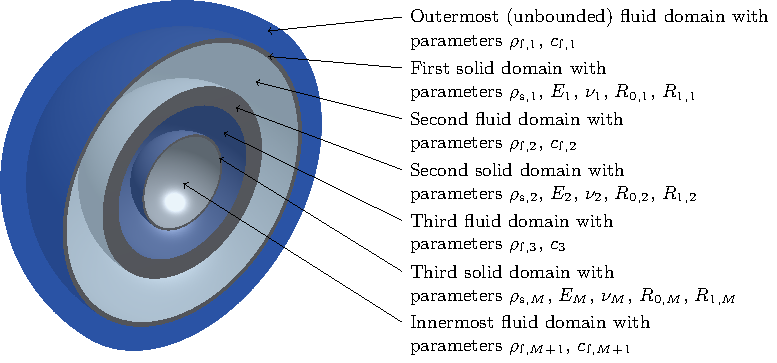
\includegraphics{parameters_distribution}
	\caption{A model with $M=3$ steel shells with different thicknesses (clip view), illustrating the distribution of the physical parameters over the different domains.}
	\label{Fig1:illustration}
\end{figure}}%

%
%%%%%%%%%%%%%%%%%%%%%%%%%%%%%%%%%%%%%%%%%%%%%%%%%%%%%%%%%%%%%%%%%%%%%%%%%%%%%%%%%%%%%%%%%%%%%%
%%% Include paper I
\paperTitle{Exact 3D Scattering Solutions for Spherical Symmetric Scatterers}%
\paperJournal{Journal of Sound and Vibration}%
\publicationStatus{Published in \textit{\the\paperJournal} (2019) \textbf{440}:439--479}%
\paperAuthors{Jon~Vegard~Ven{\aa}s and Trond~Jenserud}%
\includePaper{}{}{\label{Part:paperI}
\renewcommand{\contents}{contents/paperI}%
\begin{pFrontmatter}
    \title{Exact 3D scattering solutions for spherical\\symmetric scatterers}
	\author[a,$\ast$]{Jon Vegard Ven{\aa}s}%
	\author[b]{Trond Jenserud}%
	\address[a]{Department of Mathematical Sciences, Norwegian University of Science and Technology,\\Alfred Getz' vei 1, 7034 Trondheim, Norway}%
	\address[b]{Department of Marine Systems, Norwegian Defence Research Establishment,\\Postboks 115, 3191 Horten, Norway}%
	\eaddress[J.V. Ven{\aa}s]{Jon.Venas@ntnu.no}%
	\eaddress[T. Jenserud]{Trond.Jenserud@ffi.no}%
	\begin{abstract}%
		%Solving scattering problems using numerical steepest descent ... %\cite{Huybrechs2006mah}...
The Kirchhoff approximation yields an accurate approximation of scattering problems on convex rigid bodies for high frequencies. The Kirchhoff--Helmholtz integral has usually been evaluated by discretizing the geometry by triangles, such that the integral may be evaluated exactly. However, this approach has frequency dependent accuracy and frequency dependent memory consumption. In this work, the integrals are evaluated numerically on the exact geometry using the method of numerical steepest descent. Both problems concerning the decreased accuracy and the increased memory consumption for higher frequencies are solved by this approach. The isogeoemtric framework eliminates the tessellation process and enables computations directly on the computer aided design (CAD) model.
	\end{abstract}%
\end{pFrontmatter}



\section{Introduction}
Acoustic scattering by elastic objects is a continuing area of study. Most phenomena in the scattering process can be adequately described by linear elasticity theory, and by further restricting the analysis to homogeneous, isotropic bodies of simple geometries, the mathematical formalism becomes simple enough to be handled by conventional analytic methods. 

The problems fall into mainly three categories: scattering of acoustic waves from elastic objects, scattering of elastic waves from fluid-filled cavities and solid inclusions, and inverse scattering, i.e., obtaining properties of a scattering object from the remotely sensed field. In the first category, the classical problems include scattering by spheres and infinite cylinders: fluid spheres~\cite{Anderson1950ssf}, solid spheres and cylinders~\cite{Faran1951ssb, Anderson1955soa, Hickling1962aoe, Doolittle1968ssb, Flax1978toe, Gaunaurd1983rao}, and spherical and cylindrical shells with various combinations of material properties~\cite{Hickling1964aoe, Doolittle1966ssb, Gaunaurd1987lac, Gaunaurd1991ssb, Kaduchak1998rbm, Chang1994voa, Chang1994soa, Fender1972sfa}. 
Much of the work in this field up to around 1980, is summarized in Flax et al.~\cite{Flax1981pa}.

The surrounding medium is usually considered to be a lossless fluid, but viscous fluids~\cite{Lin1983asb} and viscoelastic media and materials~\cite{Hasheminejad2005asf} are also considered. 

The acoustic illumination is often taken to be a plane wave which is relevant for far-field sources, otherwise point sources are applied in the near-field. For the infinite cylinder, the incident field is in most cases applied normal to the cylinder, but obliquely incident fields are also considered~\cite{Bao1990ras, Daneshjou2017aes}. More recently, the problem of scattering of beams has received much attention~\cite{Marston2007abs, Gong2016aso}. 

Solutions to some non-symmetric problems are also given; e.g. partially fluid filled spheres~\cite{Fawcett2001sfa}, spheres with eccentric cavities~\cite{Hasheminejad2005asf}, and open spheres with internal point sources~\cite{Elias1991sba}.

The studies mentioned above consider a single object in the free field. It is also of interest to study interactions between objects, and between an object and a boundary. The problem of multiple scattering is studied in e.g.~\cite{Gabrielli2001asb} for two elastic spheres, and in~\cite{Wu2006mso} for many fluid spheres, while the scattering by objects close to boundaries, and by  partially buried objects is addressed in~\cite{Zampolli2009bpf}.

Applications of the theory are numerous, and include scattering from marine life~\cite{Stanton1998dbs, Stanton2000asb, Anderson1950ssf}, various aspects of sonar, nondestructive testing, seismology, detection of buried objects~\cite{Sessarego1998sba}, medical imaging~\cite{Wells2006ui}, determination of material properties by inverse scattering~\cite{Ayres1987ias}, and acoustic cloaking. Acoustic cloaking, i.e., making an object acoustically 'invisible', requires acoustic metamaterials and is difficult to realize in practice, but reducing the backscattering strength of an object is an important issue, and can be realized either passively by coating or actively as suggested in e.g. \cite{Avital2015ssa}. 
A recent area of research is noise control in aerospace- and automotive engineering, where sound transmission through cylindrical shells constructed from new composite materials \cite{Talebitooti2016att} and functionally graded materials \cite{Daneshjou2017aes} are studied in order to reduce noise level inside the cabin. The latter problem requires a full 3D solution. %Full 3D, 

The method referred to as classical scattering theory starts with the linearized elasto-dynamic equation of motion (also called Naviers equation). For the intended applications, nonlinear effects are negligible, which justifies the use of the linear approximation. For a certain class of coordinate systems, the field can be expressed in terms of three scalar potentials, which satisfy scalar Helmholtz equations, and admit solutions in the form of infinite series, termed normal modes or partial waves. The formal series expansions contain all the physical features of the solution, i.e., the reflected, transmitted and circumferential (or creeping) waves. The most general problems on finite scatterers in free space are scattering by the spherical shells which requires all three potentials and give solutions in terms of double sums. However, assuming axisymmetric illumination there is no loss of generality in aligning the coordinate axis of the sphere with the axis of the incident field, resulting in an axisymmetric problem. This results in a single infinite series which is much more computational efficient than the general case. This is the approach taken here.
 
%Truncation: 
As the solution is in the form of an infinite series, it needs to be truncated at some point. The summation is terminated when the relative magnitude of the last term is less than some prescribed tolerance, such that no computational parameters are introduced if this tolerance is chosen to be the precision used in the calculations (typically double precision). It is shown, by using symbolic precision in MATLAB, that the computational errors in the implementation are due to round-off errors. This is a natural definition of a computational exact solution.

The work reviewed above solves a host of different problems, and several reference solutions are available, with complexity up to three layers. What the present work provides is the explicit solution for a fully general multilayered sphere, and with corresponding analysis of the computational residual errors. This allows easy design and modeling of reference solutions for the purpose of validating numerical methods.
More specific, the model solves the problem of scattering by an incident plane wave, or wave from a point source, by spherical objects consisting of an arbitrary number of layers. Any combinations of fluid and solid layers can be handled, and the special cases of replacing the Neumann-to-Neumann condition by a single Neumann condition is also included.

An early work on scattering from multilayered spheres and infinite cylinders is Jenserud and Tollefsen~\cite{Jenserud1990ars}. The method employed here is referred to as the global matrix method~\cite{Schmidt1985afw} and is a systematic way of assembling local solutions for the individual layers into a global matrix for the total problem. 
The present work uses the same approach and builds mainly upon the work of Chang and Demkowicz~\cite{Chang1994voa}, which is generalized to multilayered spherical objects.

\begin{figure}
	\centering
	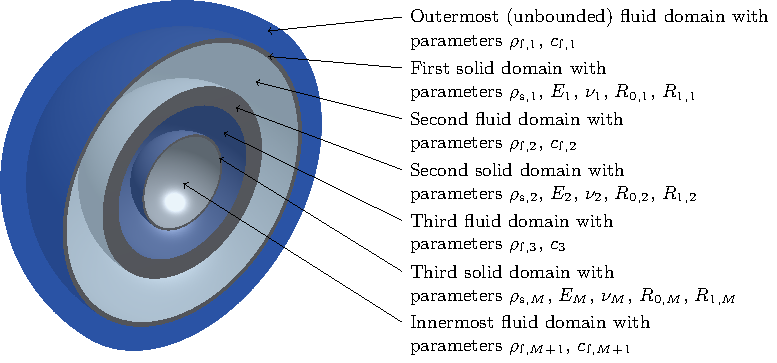
\includegraphics{parameters_distribution}
	\caption{A model with $M=3$ steel shells with different thicknesses (clip view), illustrating the distribution of the physical parameters over the different domains.}
	\label{Fig1:illustration}
\end{figure}
%\clearpage
\section{Governing equations}
\label{Sec1:govEquations}
In this section the governing equations for the problem at hand will be presented. In~\cite[pp. 13-14]{Ihlenburg1998fea} Ihlenburg briefly derives the governing equations for the acoustic-structure interaction problem. As the physical problem of interest is a time dependent problem, it is natural to first present the governing equations in the time-domain before presenting the corresponding equations in the frequency domain (obtained by Fourier transformation). It is noted right away that the fields described in this paper (both in the time-domain and frequency-domain) are all perturbation fields.

\subsection{Governing equations in the time domain}
Einstein's summation convention will be used throughout this work, such that repeated indices in products imply summation. For example, any vector $\vec{x}\in\R^3$ can be expressed as
\begin{equation}
	\vec{x}=\begin{bmatrix}
	x_1\\
	x_2\\
	x_3
\end{bmatrix} = \sum_{i=1}^3 x_i\vec{e}_i = x_i\vec{e}_i,
\end{equation}
where $\vec{e}_i\in\R^3$ is the standard basis vectors in a three-dimensional Euclidean space.

Let $\breve{\vec{u}} = \breve{u}_i\vec{e}_i$ be the time-dependent displacement field in a given solid domain, and $\breve{\vec{\sigma}}$ the corresponding stress tensor (see \Cref{Sec1:LinearElasticity} for details). Each of the components depend on the spatial variable $\vec{x}$ and the time variable $t$, such that $\breve{\vec{u}} = \breve{\vec{u}}(\vec{x},t)$. The solid domain is then governed by Navier's equation of motion~\cite{Fender1972sfa} (derived from Newton's second law) 
\begin{equation}\label{Eq1:navierTime}
	G\nabla^2\breve{\vec{u}}+\left(K+\frac{G}{3}\right)\nabla(\nabla \cdot\breve{\vec{u}}) = \rho_{\mathrm{s}}\pderiv[2]{\breve{\vec{u}}}{t},
\end{equation}
which is equivalent to~\cite[p. 223]{Slaughter2002tlt}
\begin{equation}
	\pderiv{\breve{\sigma}_{ij}}{x_j} = \rho_{\mathrm{s}}\pderiv[2]{\breve{u}_i}{t},\quad i=1,2,3.
\end{equation}
The \textit{bulk modulus}, $K$, and the \textit{shear modulus}, $G$, can be defined by the Young's modulus, $E$, and Poisson's ratio, $\nu$, as
\begin{equation}
	K = \frac{E}{3(1-2\nu)}\quad\text{and}\quad G = \frac{E}{2(1+\nu)}.
\end{equation}

Correspondingly, denote by $\breve{p}$ the time-dependent scattered pressure field in a given fluid domain, which is governed by the wave equation
\begin{equation}\label{Eq1:waveEquation}
	\nabla^2 \breve{p} = \frac{1}{c_{\mathrm{f}}^2} \pderiv[2]{\breve{p}}{t}.
\end{equation}

\subsection{Governing equations in the frequency domain}
The dimension of the governing equations may be reduced by one using a time--frequency Fourier\footnote{The sign convention in the Fourier transform differs from the classical Fourier transform~\cite{ISO2009qau}, but agrees with most literature on the subject, for example~\cite{Fender1972sfa,Ihlenburg1998fea,Jensen2011coa,Goodman1962rat}.} pair~\cite[p. 71]{Jensen2011coa}\begin{align}
	\Psi(\vec{x},\omega) = \left(\fourier\breve{\Psi}(\vec{x},\cdot)\right)(\omega) &= \int_{-\infty}^\infty \breve{\Psi}(\vec{x},t)\euler^{\imag \omega t}\idiff t\label{Eq1:Psi}\\
	\breve{\Psi}(\vec{x},t) = \left(\fourier^{-1}\Psi(\vec{x},\cdot)\right)(t)  &= \frac{1}{2\PI}\int_{-\infty}^\infty \Psi(\vec{x},\omega)\euler^{-\imag \omega t}\idiff \omega\label{Eq1:Psit}
\end{align}
where $\Psi$ represents the scattered pressure field $p$ or the displacement field $\vec{u}$. The frequency $f$ and the angular frequency $\omega$ is related by $\omega = 2\PI f$, and the angular wave number is given by $k=\omega/c_{\mathrm{f}}$.

Consider first the scattered pressure. By differentiating \Cref{Eq1:Psit} twice with respect to time, such that
\begin{equation}
	\pderiv[2]{}{t}\breve{p}(\vec{x},t) = -\omega^2\breve{p}(\vec{x},t),
\end{equation}
the following is obtained (using \Cref{Eq1:waveEquation})
\begin{align*}
	\nabla^2 p(\vec{x},\omega) + k^2 p(\vec{x},\omega) &= \int_{-\infty}^\infty \nabla^2\breve{p}(\vec{x},t)\euler^{\imag \omega t}\idiff t + \int_{-\infty}^\infty k^2 \breve{p}(\vec{x},t)\euler^{\imag \omega t}\idiff t\\
	&= \int_{-\infty}^\infty \left[\nabla^2\breve{p}(\vec{x},t)-\frac{1}{c_{\mathrm{f}}^2}\pderiv[2]{}{t}\breve{p}(\vec{x},t)\right]\euler^{\imag \omega t}\idiff t = 0.
\end{align*}
That is, $p(\vec{x},\omega)$ satisfies the Helmholtz equation
\begin{equation}\label{Eq1:helmholtz}
	\nabla^2 p + k^2p = 0.
\end{equation}
A corresponding argument shows that the displacement field $\vec{u}(\vec{x},\omega)$ satisfies
\begin{equation}\label{Eq1:navier}
	G\nabla^2\vec{u}+\left(K+\frac{G}{3}\right)\nabla(\nabla \cdot\vec{u}) +\rho_{\mathrm{s}}\omega^2\vec{u} = \zerovec.
\end{equation}
The scattered pressure, $p$, must in addition to the Helmholtz equation satisfy the Sommerfeld radiation condition for the outermost fluid layer~\cite{Sommerfeld1949pde}
\begin{equation}\label{Eq1:Sommerfeld}
	\pderiv{p(\vec{x},\omega)}{r}-\imag k p(\vec{x},\omega) = o\left(r^{-1}\right)\quad r=|\vec{x}|
\end{equation}	
as $r\to\infty$ uniformly in $\hat{\vec{x}}=\frac{\vec{x}}{r}$.

The coupling conditions (Neumann-to-Neumann) between the solid and the fluid boundaries are given by~\cite[pp. 13-14]{Ihlenburg1998fea}
\begin{align}
	\rho_{\mathrm{f}} \omega^2 u_i n_i - \pderiv{p_{\mathrm{tot}}}{n} &= 0\\
	\sigma_{ij}n_i n_j + p_{\mathrm{tot}} &= 0
\end{align}
where $\vec{n}$ is the normal vector at the surface, and $p_{\mathrm{tot}}$ is the total pressure\footnote{Since only perturbation fields are considered, $p_{\mathrm{tot}}$ does not include the static background pressure (and does therefore not represent the physical total pressure field).} (scattered pressure with the incident pressure field added for the outermost fluid). In addition, since the fluid is assumed to be ideal, there is no tangential traction at the surfaces. For spherical symmetric objects $\vec{n}=\vec{e}_{\mathrm{r}}$, such that the coupling equations reduces to
\begin{align}
	\rho_{\mathrm{f}} \omega^2 u_{\mathrm{r}} - \pderiv{p_{\mathrm{tot}}}{r} &= 0\label{Eq1:firstBC}\\
	\sigma_{\mathrm{rr}} + p_{\mathrm{tot}} &= 0\label{Eq1:secondBC}
\end{align}
in the spherical coordinate system (see \Cref{Sec1:sphericalCoordinates}). The tangential traction free boundary conditions become~\cite[p. 15]{Chang1994voa}
\begin{align}
	\sigma_{\mathrm{r}\upvartheta} &= 0\label{Eq1:traction1}\\
	\sigma_{\mathrm{r}\upvarphi} &= 0\label{Eq1:traction2}.
\end{align}
%\clearpage
\section{General solution in the solid domain}
\label{Eq1:generalSolution}
It turns out that Navier's equation can be reduced to a set of Helmholtz equations. Since the fluid domain also is governed by the Helmholtz equation, both solid and fluid domains share the same fundamental solutions, and it thus suffices to present the general solution in the solid domain.

\subsection{Lam\'{e} solution}
Fender~\cite{Fender1972sfa} shows that the solution of \Cref{Eq1:navier} can be written in terms of a scalar potential $\phi$ and a vector potential $\vec{\psi}$ as follows
\begin{equation}\label{Eq1:LameSolution}
	\vec{u} = \nabla\phi + \nabla\times\vec{\psi}.
\end{equation}
Such a solution of Navier's equation is called a Lam\'{e} solution. The potentials $\phi$ and $\vec{\psi}$ satisfy the scalar and vector Helmholtz equation, respectively. That is,
\begin{align}
	&\nabla^2\phi + a^2\phi = 0\label{Eq1:phiHelmholtz}\\
	&\nabla^2\vec{\psi} + b^2\vec{\psi} = \zerovec\label{Eq1:PsiHelmholtz}
\end{align}
where
\begin{equation}\label{Eq1:waveNumber_a_b}
	a=\frac{\omega}{c_{\mathrm{s},1}},\quad b=\frac{\omega}{c_{\mathrm{s},2}},\quad c_{\mathrm{s},1} = \sqrt{\frac{3K+4G}{3\rho_{\mathrm{s}}}},\quad c_{\mathrm{s},2} = \sqrt{\frac{G}{\rho_{\mathrm{s}}}}.
\end{equation}
Here, the parameters $c_{\mathrm{s},1}$ and $c_{\mathrm{s},2}$ are the longitudinal and transverse (elastic) wave velocities, respectively, and $a$ and $b$ are the corresponding angular wave numbers in the solid. 

Throughout this work, axisymmetry around the $x_3$-axis is assumed. Assuming symmetry around this particular axis causes no loss of generality, as both the incident wave and the spherical shell share this symmetry property (a simple orthogonal transformation restores the generality of axisymmetry about an arbitrary axis). In the spherical coordinate system, the pressure $p$ and the displacement $\vec{u}$ are then independent of the azimuth angle $\varphi$ in the fluid and solid domains, respectively. Moreover, the solid component in the azimuth angle direction is zero, $u_\upvarphi=0$. This is a result of the axisymmetry of the problem.

\subsection{Series representation using separation of variables}
Using these assumptions Fender~\cite{Fender1972sfa} shows that $\vec{\psi}=\psi_\upvarphi\vec{e}_\upvarphi$, such that when \Cref{Eq1:phiHelmholtz,Eq1:PsiHelmholtz} are expanded in terms of spherical coordinates, the following is obtained (using \Cref{Eq1:laplaceScalarSpherical,Eq1:LapVecPotSpherical})
\begin{align}
	\pderiv{}{r}\left(r^2\pderiv{\phi}{r}\right) + \frac{1}{\sin\vartheta}\pderiv{}{\vartheta}\left(\sin\vartheta\pderiv{\phi}{\vartheta}\right) + (ar)^2\phi &= 0\\
	\pderiv{}{r}\left(r^2\pderiv{\psi_\upvarphi}{r}\right) + \frac{1}{\sin\vartheta}\pderiv{}{\vartheta}\left(\sin\vartheta\pderiv{\psi_\upvarphi}{\vartheta}\right) + \left[(br)^2-\frac{1}{\sin^2\vartheta}\right]\psi_\upvarphi &= 0.
\end{align}
Using separation of variables, each of these equations can be reduced to a couple of spherical Bessel and Legendre equations, with the associate Legendre polynomials of zero and first order (described in \Cref{subsec:legendre}) and spherical Bessel functions (described in \Cref{subsec:sphericalBesselAndHankel}) as solutions. More explicitly,
\begin{align}
	\phi(r,\vartheta) &= \sum_{n=0}^\infty \legendre_n(\cos\vartheta)\left[A_n^{(1)}\besselj_n(ar)+A_n^{(2)}\bessely_n(ar)\right]\label{Eq1:phiSolution}\\
	\psi_\upvarphi(r,\vartheta) &= \sum_{n=0}^\infty \legendre_n^1(\cos\vartheta)\left[B_n^{(1)}\besselj_n(br)+B_n^{(2)}\bessely_n(br)\right]\label{Eq1:psiSolution}
\end{align}
where the coefficients $A_n^{(i)},B_n^{(i)}\in\C$, $i=1,2$, are chosen such that the boundary conditions are satisfied.

By using \Cref{Eq1:LegendreRelation1} these functions and their partial derivatives will have their $\vartheta$-dependency contained in functions of the form (the ones relevant for this work are listed in \Cref{Eq1:Qs})
\begin{equation}
	Q_n^{(j)}(\vartheta) = \deriv[j]{}{\vartheta}\legendre_n(\cos\vartheta).
\end{equation}
That is, there is no need for the associated Legendre polynomials.

For ease of notation, the function $Z_n^{(i)}(\zeta)$, $i=1,2$, is introduced (as in~\cite{Chang1994voa, Chang1994soa}), where 
\begin{equation}
	Z_n^{(1)}(\zeta) = \besselj_n(\zeta),\quad Z_n^{(2)}(\zeta) = \bessely_n(\zeta).
\end{equation}
Moreover, the notation $\xi = \xi(r) = ar$ and $\eta = \eta(r) = br$ is used for convenience. Using the Einstein summation convention, \Cref{Eq1:phiSolution,Eq1:psiSolution} may now be rewritten as
\begin{align}
	\phi(r,\vartheta) &= \sum_{n=0}^\infty Q_n^{(0)}(\vartheta)A_n^{(i)}Z_n^{(i)}(\xi)\label{Eq1:phiSolutionSimplified}\\
	\psi_\upvarphi(r,\vartheta) &= \sum_{n=0}^\infty Q_n^{(1)}(\vartheta)B_n^{(i)}Z_n^{(i)}(\eta).\label{Eq1:psiSolutionSimplified}
\end{align}

\subsection{Expressions for the displacement and stress field}
By expanding \Cref{Eq1:LameSolution} in spherical coordinates (using \Cref{Eq1:delScalarSpherical,Eq1:CrossVecPotSpherical}) yields
\begin{equation}
	\vec{u} = \nabla\phi + \nabla\times\vec{\psi} = \pderiv{\phi}{r}\vec{e}_{\mathrm{r}} + \frac{1}{r}\pderiv{\phi}{\vartheta}\vec{e}_{\upvartheta} + \frac{1}{r\sin\vartheta}\pderiv{}{\vartheta}\left(\psi_\upvarphi\sin\vartheta\right)\vec{e}_{\mathrm{r}} - \frac{1}{r}\pderiv{}{r}\left(r\psi_\upvarphi\right)\vec{e}_{\upvartheta} 
\end{equation}
such that
\begin{equation}
	u_{\mathrm{r}} = \pderiv{\phi}{r} + \frac{1}{r}\pderiv{\psi_\upvarphi}{\vartheta} + \frac{1}{r}\psi_\upvarphi\cot\vartheta
\end{equation}
and
\begin{equation}
	u_\upvartheta = \frac{1}{r}\pderiv{\phi}{\vartheta} -\pderiv{\psi_\upvarphi}{r} -\frac{1}{r}\psi_\upvarphi.
\end{equation}
Insertion of \Cref{Eq1:phiSolutionSimplified,Eq1:psiSolutionSimplified} (using \Cref{Eq1:expandedLegendreEquationIdentity,Eq1:LegendreRelation1,Eq1:BesselDerivIdentity2})
yields
\begin{equation}\label{Eq1:u_rgen}
	u_{\mathrm{r}} = \frac{1}{r}\sum_{n=0}^\infty Q_n^{(0)}(\vartheta)\left[A_n^{(i)}S_{1,n}^{(i)}(\xi)+B_n^{(i)}T_{1,n}^{(i)}(\eta)\right]
\end{equation}
and
\begin{equation}\label{Eq1:u_tgen}
	u_\upvartheta = \frac{1}{r}\sum_{n=0}^\infty Q_n^{(1)}(\vartheta)\left[A_n^{(i)}S_{2,n}^{(i)}(\xi)+B_n^{(i)}T_{2,n}^{(i)}(\eta)\right]
\end{equation}
where
\begin{align*}
	S_{1,n}^{(i)}(\xi) &= \xi \deriv{}{\xi}Z_n^{(i)}(\xi) =  nZ_n^{(i)}(\xi)-\xi Z_{n+1}^{(i)}(\xi)\\ 
	T_{1,n}^{(i)}(\eta) &= -n(n+1)Z_n^{(i)}(\eta)\\
	S_{2,n}^{(i)}(\xi) &= Z_n^{(i)}(\xi)\\
	T_{2,n}^{(i)}(\eta) &= -Z_n^{(i)}(\eta)-\eta \deriv{}{\eta}Z_n^{(i)}(\eta) = -(n+1)Z_n^{(i)}(\eta) + \eta Z_{n+1}^{(i)}(\eta).
\end{align*}
To compute the stresses defined in \Cref{Sec1:sphericalCoordinates}, the partial derivatives of the displacement field in the spherical coordinate system are needed. These derivatives are found to be (using \Cref{Eq1:expandedLegendreEquationIdentity2,Eq1:BesselDerivIdentity1,Eq1:BesselDerivIdentity2})
\begin{align}
	\pderiv{u_{\mathrm{r}}}{r} &= \frac{1}{r^2}\sum_{n=0}^\infty Q_n^{(0)}(\vartheta)\left[A_n^{(i)}S_{3,n}^{(i)}(\xi)+B_n^{(i)}T_{3,n}^{(i)}(\eta)\right]\\
	\pderiv{u_{\upvartheta}}{r} &= \frac{1}{r^2}\sum_{n=0}^\infty Q_n^{(1)}(\vartheta)\left[A_n^{(i)}S_{4,n}^{(i)}(\xi)+B_n^{(i)}T_{4,n}^{(i)}(\eta)\right]\\
	\pderiv{u_{\mathrm{r}}}{\vartheta} &= \frac{1}{r}\sum_{n=0}^\infty Q_n^{(1)}(\vartheta)\left[A_n^{(i)}S_{1,n}^{(i)}(\xi)+B_n^{(i)}T_{1,n}^{(i)}(\eta)\right]\\
	\pderiv{u_\upvartheta}{\vartheta} &= \frac{1}{r}\sum_{n=0}^\infty Q_n^{(2)}(\vartheta)\left[A_n^{(i)}S_{2,n}^{(i)}(\xi)+B_n^{(i)}T_{2,n}^{(i)}(\eta)\right]
\end{align}
where
\begin{align*}
	S_{3,n}^{(i)}(\xi) &= \xi \deriv{}{\xi}S_{1,n}^{(i)}(\xi) - S_{1,n}^{(i)}(\xi) =  (n^2-\xi^2-n)Z_n^{(i)}(\xi) + 2\xi Z_{n+1}^{(i)}(\xi)\\ 
	T_{3,n}^{(i)}(\eta) &= \eta \deriv{}{\eta}T_{1,n}^{(i)}(\eta) -T_{1,n}^{(i)}(\eta) = -n(n+1)\left[(n-1)Z_n^{(i)}(\eta) - \eta Z_{n+1}^{(i)}(\eta)\right]\\
	S_{4,n}^{(i)}(\xi) &= \xi \deriv{}{\xi}Z_n^{(i)}(\xi) - Z_n^{(i)}(\xi) = (n-1)Z_n^{(i)}(\xi)-\xi Z_{n+1}^{(i)}(\xi)\\ 
	T_{4,n}^{(i)}(\eta) &= \eta\deriv{}{\eta}T_{2,n}^{(i)}(\eta) - T_{2,n}^{(i)}(\eta) = (\eta^2-n^2+1)Z_n^{(i)}(\eta) -\eta Z_{n+1}^{(i)}(\eta).
\end{align*}
Using \Cref{Eq1:constitutiveRelationSpherical,Eq1:strainsInSpherical}, and the relation\footnote{This relation is obtained by inserting the definition of the angular wave numbers $a$ and $b$ (\Cref{Eq1:waveNumber_a_b}) into the left-hand side.}
\begin{equation}
	\frac{1}{2}\left(\frac{b}{a}\right)^2 = \frac23+\frac{K}{2G}
\end{equation}
the following formulas for the stress field components are obtained\footnote{One can save some work by observing the similarities between $\sigma_{\upvartheta\upvartheta}$ and $\sigma_{\upvarphi\upvarphi}$
\begin{align*}
	\sigma_{\upvartheta\upvartheta} &= \frac{2}{r}\left(K+\frac{G}{3}\right)u_{\mathrm{r}} + \left(K-\frac{2G}{3}\right)\pderiv{u_{\mathrm{r}}}{r} + \frac{3K-2G}{3r}\left(u_\upvartheta\cot\vartheta + \pderiv{u_\upvartheta}{\vartheta}\right) + \frac{2G}{r}\pderiv{u_\upvartheta}{\vartheta}\\
	\sigma_{\upvarphi\upvarphi} &= \frac{2}{r}\left(K+\frac{G}{3}\right)u_{\mathrm{r}} + \left(K-\frac{2G}{3}\right)\pderiv{u_{\mathrm{r}}}{r} + \frac{3K-2G}{3r}\left(u_\upvartheta\cot\vartheta + \pderiv{u_\upvartheta}{\vartheta}\right) + \frac{2G}{r} u_\upvartheta\cot\vartheta.
\end{align*}}
\begin{align}\label{Eq1:stressFieldComponents1}
	\sigma_{\mathrm{r}\mathrm{r}} &= \frac{2G}{r^2}\sum_{n=0}^\infty Q_n^{(0)}(\vartheta)\left[A_n^{(i)} S_{5,n}^{(i)}(\xi) + B_n^{(i)} T_{5,n}^{(i)}(\eta)\right]\\\label{Eq1:stressFieldComponents4}
	\sigma_{\upvartheta\upvarphi} &= 0\\\label{Eq1:stressFieldComponents5}
	\sigma_{\mathrm{r}\upvarphi} &= 0
\end{align}
\begin{align}
	\sigma_{\upvartheta\upvartheta} &= \frac{2G}{r^2}\sum_{n=0}^\infty\left\{Q_n^{(0)}(\vartheta)\left[A_n^{(i)} S_{6,n}^{(i)}(\xi) + B_n^{(i)} T_{6,n}^{(i)}(\eta)\right]\right.\nonumber\\ \label{Eq1:stressFieldComponents2}
	&{\hskip5em\relax}\left.+  Q_n^{(2)}(\vartheta)\left[A_n^{(i)} S_{2,n}^{(i)}(\xi) + B_n^{(i)} T_{2,n}^{(i)}(\eta)\right]\right\}\\
	\sigma_{\upvarphi\upvarphi} &= \frac{2G}{r^2}\sum_{n=0}^\infty\left\{Q_n^{(0)}(\vartheta)\left[A_n^{(i)} S_{6,n}^{(i)}(\xi) + B_n^{(i)} T_{6,n}^{(i)}(\eta)\right]\right.\nonumber\\ \label{Eq1:stressFieldComponents3}
	&{\hskip5em\relax}\left. +   Q_n^{(1)}(\vartheta)\cot(\vartheta)\left[A_n^{(i)} S_{2,n}^{(i)}(\xi) + B_n^{(i)} T_{2,n}^{(i)}(\eta)\right]\right\}\\\label{Eq1:stressFieldComponents6}
	\sigma_{\mathrm{r}\upvartheta} &= \frac{2G}{r^2}\sum_{n=0}^\infty Q_n^{(1)}(\vartheta)\left[A_n^{(i)} S_{7,n}^{(i)}(\xi) + B_n^{(i)} T_{7,n}^{(i)}(\eta)\right]
\end{align}
where
\begin{align}\label{Eq1:stress}
\begin{split}
	S_{5,n}^{(i)}(\xi) &= \frac{1}{2G}\left[\left(K+\frac{4G}{3}\right)S_{3,n}^{(i)}(\xi) - \left(K-\frac{2G}{3}\right) n(n+1)Z_n^{(i)}(\xi)\right.\\ 
	&{\hskip4em\relax}\left. + 2\left(K-\frac{2G}{3}\right) S_{1,n}^{(i)}(\xi)\right] \\
	&= \left[n^2-n-\frac{1}{2}\left(\frac{b}{a}\right)^2\xi^2\right] Z_n^{(i)}(\xi) + 2\xi Z_{n+1}^{(i)}(\xi)\\
	T_{5,n}^{(i)}(\eta) &= \frac{1}{2G}\left[\left(K+\frac{4G}{3}\right)T_{3,n}^{(i)}(\eta) - \left(K-\frac{2G}{3}\right) n(n+1)T_{2,n}^{(i)}(\eta)\right.\\ 
	&{\hskip4em\relax}\left. + 2\left(K-\frac{2G}{3}\right) T_{1,n}^{(i)}(\eta)\right] \\
	&= -n(n+1)\left[(n-1)Z_n^{(i)}(\eta) - \eta Z_{n+1}^{(i)}(\eta)\right]\\
	S_{6,n}^{(i)}(\xi) &= -\left(\frac{K}{2G}-\frac13\right)n(n+1)S_{2,n}^{(i)}(\xi) +\left(\frac13+\frac{K}{G} \right)S_{1,n}^{(i)}(\xi) + \left(\frac{K}{2G}-\frac13\right)S_{3,n}^{(i)}(\xi)\\
	&= \left[n-\frac{1}{2}\left(\frac{b}{a}\right)^2\xi^2+\xi^2\right] Z_n^{(i)}(\xi) - \xi Z_{n+1}^{(i)}(\xi)\\
	T_{6,n}^{(i)}(\eta) &=  -\left(\frac{K}{2G}-\frac13\right)n(n+1)T_{2,n}^{(i)}(\eta) +\left(\frac13+\frac{K}{G} \right)T_{1,n}^{(i)}(\eta) + \left(\frac{K}{2G}-\frac13\right)T_{3,n}^{(i)}(\eta)\\
	&= -n(n+1)Z_n^{(i)}(\eta)\\
	S_{7,n}^{(i)}(\xi) &= \frac{1}{2}\left[S_{1,n}^{(i)}(\xi) + S_{4,n}^{(i)}(\xi) - S_{2,n}^{(i)}(\xi) \right] \\
	&= (n-1)Z_n^{(i)}(\xi) -\xi Z_{n+1}^{(i)}(\xi)\\
	T_{7,n}^{(i)}(\eta) &= \frac{1}{2}\left[T_{1,n}^{(i)}(\eta) + T_{4,n}^{(i)}(\eta) - T_{2,n}^{(i)}(\eta) \right] \\
	&= -\left(n^2-1-\frac{1}{2}\eta^2\right)Z_n^{(i)}(\eta) - \eta Z_{n+1}^{(i)}(\xi).
	\end{split}
\end{align}
%
\subsection{Validation of the displacement and stress formulas}
The correctness of the formulas may be controlled by considering Navier's equation (\Cref{Eq1:navier}) in spherical coordinates. The three components of Navier's equation in spherical coordinates are given in \Cref{Eq1:navierSpherical1,Eq1:navierSpherical2,Eq1:navierSpherical3}, the last of which is automatically satisfied due to the symmetry assumptions. The first two equations simplify to
%\begin{align}\label{Eq1:navierSphericalSimplified1}%
%\pderiv{\sigma_{\mathrm{rr}}}{r} + \frac{1}{r}\pderiv{\sigma_{\mathrm{r}\upvartheta}}{\vartheta} + \frac{1}{r}\left(2\sigma_{\mathrm{r}\mathrm{r}} - \sigma_{\upvartheta\upvartheta} - \sigma_{\upvarphi\upvarphi} + \sigma_{\mathrm{r}\upvartheta}\cot\vartheta\right) +\omega^2\rho_{\mathrm{s}}u_{\mathrm{r}} &= 0\\
%	\pderiv{\sigma_{\mathrm{r}\upvartheta}}{r} + \frac{1}{r}\pderiv{\sigma_{\upvartheta\upvartheta}}{\vartheta} + \frac{1}{r}\left[(\sigma_{\upvartheta\upvartheta} - \sigma_{\upvarphi\upvarphi})\cot\vartheta + 3\sigma_{\mathrm{r}\upvartheta} \right] +\omega^2\rho_{\mathrm{s}}u_\upvartheta &= 0.\label{Eq1:navierSphericalSimplified2}
%\end{align}
\begin{equation}\label{Eq1:navierSphericalSimplified1}%
\pderiv{\sigma_{\mathrm{rr}}}{r} + \frac{1}{r}\pderiv{\sigma_{\mathrm{r}\upvartheta}}{\vartheta} + \frac{1}{r}\left(2\sigma_{\mathrm{r}\mathrm{r}} - \sigma_{\upvartheta\upvartheta} - \sigma_{\upvarphi\upvarphi} + \sigma_{\mathrm{r}\upvartheta}\cot\vartheta\right) +\omega^2\rho_{\mathrm{s}}u_{\mathrm{r}} = 0
\end{equation}
and
\begin{equation}\label{Eq1:navierSphericalSimplified2}
\pderiv{\sigma_{\mathrm{r}\upvartheta}}{r} + \frac{1}{r}\pderiv{\sigma_{\upvartheta\upvartheta}}{\vartheta} + \frac{1}{r}\left[(\sigma_{\upvartheta\upvartheta} - \sigma_{\upvarphi\upvarphi})\cot\vartheta + 3\sigma_{\mathrm{r}\upvartheta} \right] +\omega^2\rho_{\mathrm{s}}u_\upvartheta = 0.
\end{equation}
Differentiation of the stress field components yields
\begin{align*}
	\pderiv{\sigma_{\mathrm{r}\mathrm{r}}}{r} &= \frac{2G}{r^3}\sum_{n=0}^\infty Q_n^{(0)}(\vartheta)\left[A_n^{(i)} S_{8,n}^{(i)}(\xi) + B_n^{(i)} T_{8,n}^{(i)}(\eta)\right]\\
	\pderiv{\sigma_{\upvartheta\upvartheta}}{\vartheta} &= \frac{2G}{r^2}\sum_{n=0}^\infty\left\{Q_n^{(1)}(\vartheta)\left[A_n^{(i)} S_{6,n}^{(i)}(\xi) + B_n^{(i)} T_{6,n}^{(i)}(\eta)\right] \right.\\ 
	&{\hskip5em\relax}\left. +  Q_n^{(3)}(\vartheta)\left[A_n^{(i)} S_{2,n}^{(i)}(\xi) + B_n^{(i)} T_{2,n}^{(i)}(\eta)\right]\right\}\\
	\pderiv{\sigma_{\mathrm{r}\upvartheta}}{r} &= \frac{2G}{r^3}\sum_{n=0}^\infty Q_n^{(1)}(\vartheta)\left[A_n^{(i)} S_{9,n}^{(i)}(\xi) + B_n^{(i)} T_{9,n}^{(i)}(\eta)\right]\\
	\pderiv{\sigma_{\mathrm{r}\upvartheta}}{\vartheta} &= \frac{2G}{r^2}\sum_{n=0}^\infty Q_n^{(2)}(\vartheta)\left[A_n^{(i)} S_{7,n}^{(i)}(\xi) + B_n^{(i)} T_{7,n}^{(i)}(\eta)\right]
\end{align*}
where
\begin{align*}
	S_{8,n}^{(i)}(\xi) &= -2S_{5,n}^{(i)}(\xi) + \xi \deriv{}{\xi}S_{5,n}^{(i)}(\xi) \\
	&= \left[n^3-3n^2+2n-\frac{n}{2}\left(\frac{b}{a}\right)^2\xi^2 + 2\xi^2\right]Z_n^{(i)}(\xi)\\ 
	&{\hskip1em\relax} + \left[-n^2-n-6+\frac{1}{2}\left(\frac{b}{a}\right)^2\xi^2\right]\xi Z_{n+1}^{(i)}(\xi)\\
	T_{8,n}^{(i)}(\eta) &= -2T_{5,n}^{(i)}(\eta) + \eta \deriv{}{\eta}T_{5,n}^{(i)}(\eta) \\
	&= n(n+1)\left[\left(-n^2+3n-2+\eta^2\right)Z_n^{(i)}(\eta) - 4\eta Z_{n+1}^{(i)}(\eta)\right]\\
	S_{9,n}^{(i)}(\xi) &= -2S_{7,n}^{(i)}(\xi) + \xi \deriv{}{\xi}S_{7,n}^{(i)}(\xi) \\
	&= \left[n^2-3n+2-\xi^2\right]Z_n^{(i)}(\xi) + 4\xi Z_{n+1}^{(i)}(\xi) \\
\end{align*}
\begin{align*}
	T_{9,n}^{(i)}(\eta) &= -2T_{7,n}^{(i)}(\eta) + \eta \deriv{}{\eta}T_{7,n}^{(i)}(\eta) \\
	&= \left(-n^3+2n^2+n-2+\frac{n}{2}\eta^2-\eta^2\right)Z_n^{(i)}(\eta)\\ 
	&{\hskip1em\relax} +\left(n^2+n+2-\frac{1}{2}\eta^2\right)\eta Z_{n+1}^{(i)}(\eta).
\end{align*}
Inserting these expressions (alongside the stress components in \Cref{Eq1:stressFieldComponents1,Eq1:stressFieldComponents2,Eq1:stressFieldComponents3,Eq1:stressFieldComponents4,Eq1:stressFieldComponents5,Eq1:stressFieldComponents6}) into \Cref{Eq1:navierSphericalSimplified1,Eq1:navierSphericalSimplified2} and using \Cref{Eq1:expandedLegendreEquationIdentity2,Eq1:expandedLegendreEquationIdentity3}, and observing that
\begin{align*}
	\pderiv{\sigma_{\upvartheta\upvartheta}}{\vartheta} +(\sigma_{\upvartheta\upvartheta} - \sigma_{\upvarphi\upvarphi})\cot\vartheta= \frac{2G}{r^2}&\sum_{n=0}^\infty  Q_n^{(1)}(\vartheta)\left\{A_n^{(i)} S_{6,n}^{(i)}(\xi) + B_n^{(i)} T_{6,n}^{(i)}(\eta)\right. \\
	&{\hskip1em\relax}+\left. \left(-n^2-n+1\right)\left[A_n^{(i)} S_{2,n}^{(i)}(\xi) + B_n^{(i)} T_{2,n}^{(i)}(\eta)\right]\right\},
\end{align*}
the left-hand side of \Cref{Eq1:navierSphericalSimplified1} and \Cref{Eq1:navierSphericalSimplified2} are indeed equal to zero.

%%\clearpage
\section{Establishing constraints from boundary conditions}
\label{Sec1:estabConstraints}
As the solution is represented as an infinite sum, the coefficients $A_{m,n}^{(i)}$, $B_{m,n}^{(i)}$ and $C_{m,n}^{(i)}$ (coefficients from the fluid domains described below) must be computed for each $n$ (see \Cref{Fig1:coefficients}). By enforcing the boundary conditions in \Cref{Eq1:firstBC,Eq1:secondBC} at each surface, constraints are developed to establish expressions for these coefficients.

\subsection{Notation for the solution in layered domains}
For the $m^{\mathrm{th}}$ solid shell the displacement field from \Cref{Eq1:u_rgen,Eq1:u_tgen} is written as
\begin{equation}
	\vec{u}_m = u_{\mathrm{r},m} \vec{e}_{\mathrm{r}} + u_{\upvartheta,m} \vec{e}_\upvartheta
\end{equation}
where
\begin{align}
	u_{\mathrm{r},m}(r,\vartheta) &= \sum_{n=0}^\infty Q_n^{(0)}(\vartheta)u_{\mathrm{r},m,n}(r) \label{Eq1:u_r}\\
	u_{\upvartheta,m}(r,\vartheta) &= \sum_{n=0}^\infty Q_n^{(1)}(\vartheta)u_{\upvartheta,m,n}(r)
\end{align}
and 
\begin{figure}
	\centering
	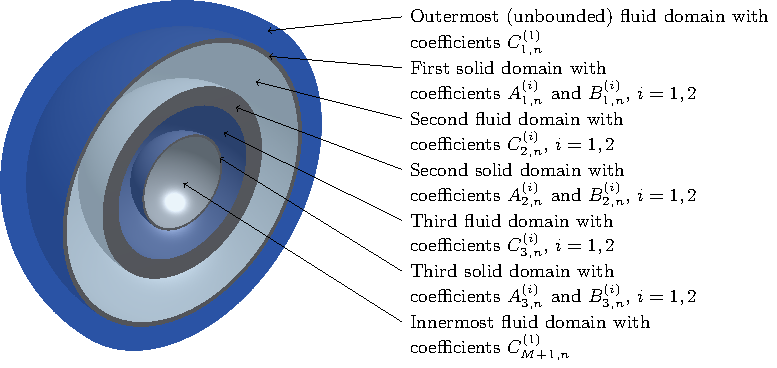
\includegraphics{coefficients_distribution}
	\caption{A model with $M=3$ steel shells with different thicknesses (clip view), illustrating the distribution of the coefficients $A_{m,n}^{(i)}$, $B_{m,n}^{(i)}$ and $C_{m,n}^{(i)}$ over the different domains.}
	\label{Fig1:coefficients}
\end{figure}
\begin{align}
	u_{\mathrm{r},m,n}(r) &= \frac{1}{r}\left[A_{m,n}^{(i)}S_{1,n}^{(i)}(a_m r)+B_{m,n}^{(i)}T_{1,n}^{(i)}(b_m r)\right]\\
	u_{\upvartheta,m,n}(r) &= \frac{1}{r}\left[A_{m,n}^{(i)}S_{2,n}^{(i)}(a_m r)+B_{m,n}^{(i)}T_{2,n}^{(i)}(b_m r)\right].
\end{align}
Corresponding expressions for the stress field in \Cref{Eq1:stress} are obtained as
\begin{align}
	\sigma_{\mathrm{rr},m}(r,\vartheta) &= \sum_{n=0}^\infty Q_n^{(0)}(\vartheta)\sigma_{\mathrm{rr},m,n}(r)\label{Eq1:sigma_rr}\\
	\sigma_{\upvartheta\upvartheta,m}(r,\vartheta) &= \sum_{n=0}^\infty Q_n^{(0)}(\vartheta)\sigma_{\upvartheta\upvartheta,m,n}^{(1)}(r) + Q_n^{(2)}(\vartheta)\sigma_{\upvartheta\upvartheta,m,n}^{(2)}(r)\\
	\sigma_{\upvarphi\upvarphi,m}(r,\vartheta) &= \sum_{n=0}^\infty Q_n^{(0)}(\vartheta)\sigma_{\upvarphi\upvarphi,m,n}^{(1)}(r) +  Q_n^{(1)}(\vartheta)\cot(\vartheta)\sigma_{\upvarphi\upvarphi,m,n}^{(2)}(r)\\
	\sigma_{\mathrm{r}\upvarphi,m}(r,\vartheta) &= 0\\
	\sigma_{\upvartheta\upvarphi,m}(r,\vartheta) &= 0\\
	\sigma_{\mathrm{r}\upvartheta,m}(r,\vartheta) &= \sum_{n=0}^\infty Q_n^{(1)}(\vartheta)\sigma_{\mathrm{r}\upvartheta,m,n}(r)\label{Eq1:sigma_rt}
\end{align}
where
\begin{align*}
	\sigma_{\mathrm{rr},m,n}(r) &= \frac{2G_m}{r^2}\left[A_{m,n}^{(i)} S_{5,n}^{(i)}(a_m r) + B_{m,n}^{(i)} T_{5,n}^{(i)}(b_m r)\right]\\
	\sigma_{\upvartheta\upvartheta,m,n}^{(1)}(r) &= \frac{2G_m}{r^2}\left[A_{m,n}^{(i)} S_{6,n}^{(i)}(a_m r) + B_{m,n}^{(i)} T_{6,n}^{(i)}(b_m r)\right]\\
	\sigma_{\upvartheta\upvartheta,m,n}^{(2)}(r) &= \frac{2G_m}{r^2}\left[A_{m,n}^{(i)} S_{2,n}^{(i)}(a_m r) + B_{m,n}^{(i)} T_{2,n}^{(i)}(b_m r)\right]\\ 
\end{align*}
\begin{align*}
	\sigma_{\upvarphi\upvarphi,m,n}^{(1)}(r) &= \frac{2G_m}{r^2}\left[A_{m,n}^{(i)} S_{6,n}^{(i)}(a_m r) + B_{m,n}^{(i)} T_{6,n}^{(i)}(b_m r)\right]\\
	\sigma_{\upvarphi\upvarphi,m,n}^{(2)}(r) &= \frac{2G_m}{r^2}\left[A_{m,n}^{(i)} S_{2,n}^{(i)}(a_m r) + B_{m,n}^{(i)} T_{2,n}^{(i)}(b_m r)\right]\\ 
	\sigma_{\mathrm{r}\upvartheta,m,n}(r) &= \frac{2G_m}{r^2}\left[A_{m,n}^{(i)} S_{7,n}^{(i)}(a_m r) + B_{m,n}^{(i)} T_{7,n}^{(i)}(b_m r)\right].
\end{align*}

The solution to the Helmholtz equation in the $m^{\mathrm{th}}$ fluid domain (for $2 \leq m \leq M$) has the same general form as $\phi$ in \Cref{Eq1:phiSolutionSimplified}
\begin{equation}\label{Eq1:generalSol}
	p_m(r,\vartheta) = \sum_{n=0}^\infty Q_n^{(0)}(\vartheta)C_{m,n}^{(i)} Z_n^{(i)}(k_m r)
\end{equation}
where the coefficients $C_{m,n}^{(i)}\in\C$ are chosen such that the boundary conditions are satisfied. As the spherical Hankel functions of first and second kind (described in  \Cref{subsec:sphericalBesselAndHankel}) are linear combinations of the spherical Bessel functions of first and second kind, the general solution can be written in terms of these functions. For the outer (unbounded) fluid the Hankel function of the second kind is eliminated due to the Sommerfeld radiation condition in \Cref{Eq1:Sommerfeld}~\cite[p. 26]{Ihlenburg1998fea}. Thus, for the outermost fluid, the scattered pressure field is given by
\begin{equation}\label{Eq1:outerFluid}
	p_1(r,\vartheta) = \sum_{n=0}^\infty Q_n^{(0)}(\vartheta) C_{1,n}^{(1)} \hankel^{(1)}_n(k_1 r).
\end{equation}
Moreover, it is required that the pressure in the innermost fluid domain is\linebreak bounded~\cite[p. 10]{Fender1972sfa}. Hence, the coefficients $C_{M+1,n}^{(2)}$ must be set to zero as the spherical Bessel function of second kind is unbounded at the origin. The pressure in the innermost fluid is therefore given by (cf.~\cite[p. 10]{Fender1972sfa})
\begin{equation}\label{Eq1:innerFluid}
	p_{M+1}(r,\vartheta) = \sum_{n=0}^\infty Q_n^{(0)}(\vartheta) C_{M+1,n}^{(1)} \besselj_n(k_{M+1} r).
\end{equation}
The total pressure in the $m^{\mathrm{th}}$ fluid domain shall be denoted by
\begin{equation}\label{Eq1:totPressure}
	p_{\mathrm{tot},m} =\begin{cases}
	p_1 + p_{\mathrm{inc}}& m = 1\\
	p_m & \text{otherwise}
	\end{cases}	
\end{equation}
where $p_{\mathrm{inc}}$ is the incident wave.

If the coefficients $A_{m,n}^{(i)}$, $B_{m,n}^{(i)}$ and $C_{m,n}^{(i)}$ can be determined, the solution is fully determined in all domains. Hence, a system of equations will be developed to find these coefficients. Indeed, at the boundaries (at a fixed radius) the series can all be written in terms of the Legendre functions $\legendre_n(\cos\vartheta)$, such that the resulting coefficients can be compared for each $n$. A term in the solution is often referred to as a \textit{mode}, such that the resulting constraints from the boundary conditions form a set of \textit{modal equations}. The terminology comes from the vibration analysis~\cite{Chang1994voa}, where each of these modes represent vibration modes. For example, $u_{\mathrm{r},m,n}$ is referred to be the radial displacement in the $m^{\mathrm{th}}$ solid domain in the $n^{\mathrm{th}}$ mode.

\subsection{Tangential traction conditions}
\Cref{Eq1:traction2} is automatically fulfilled due to the axisymmetric assumption. For the $m^{\mathrm{th}}$ shell, evaluating \Cref{Eq1:traction1} at both the inner and outer radius, yields two equations 
\begin{equation}\label{Eq1:tractionCondInserted}
	\sigma_{\mathrm{r}\upvartheta,m,n}(R_{j,m},\vartheta) = 0, \quad j=0,1.
\end{equation}
As $Q_0^{(1)}(\vartheta)=0$, these equations are automatically satisfied for $n=0$. In addition, since $T_{1,0}^{(i)}(\eta)=0$ and $T_{6,0}^{(i)}(\eta)=0$, the coefficients $B_{m,0}^{(i)}$ are redundant (which is convenient, as two constraints are lost in this case). 

Denote by $\vec{H}_{m,n}^{(1)}$, $m=1,\dots,M$, the eigenfrequency matrix\footnote{As illustrated in~\cite{Chang1994voa}, the matrix $\vec{H}_{m,n}^{(1)}$ represent the modal characteristic equations of the $m^{\mathrm{th}}$ shell. That is, the eigenfrequencies of each shell can be found by solving $\det\vec{H}_{m,n}^{(1)}=0$ in terms of the frequency.}~\cite[p. 17]{Chang1994voa} of the $m^{\mathrm{th}}$ shell
\begin{equation}\label{Eq1:K1n}
	\vec{H}_{m,n}^{(1)} = \begin{bmatrix} S_{5,n}^{(1)}(a_m R_{0,m}) & S_{5,n}^{(2)}(a_m R_{0,m}) & T_{5,n}^{(1)}(b_m R_{0,m}) & T_{5,n}^{(2)}(b_m R_{0,m})\\
	S_{7,n}^{(1)}(a_m R_{0,m}) & S_{7,n}^{(2)}(a_m R_{0,m}) & T_{7,n}^{(1)}(b_m R_{0,m}) & T_{7,n}^{(2)}(b_m R_{0,m})\\
	S_{7,n}^{(1)}(a_m R_{1,m}) & S_{7,n}^{(2)}(a_m R_{1,m}) & T_{7,n}^{(1)}(b_m R_{1,m}) & T_{7,n}^{(2)}(b_m R_{1,m})\\
	S_{5,n}^{(1)}(a_m R_{1,m}) & S_{5,n}^{(2)}(a_m R_{1,m}) & T_{5,n}^{(1)}(b_m R_{1,m}) & T_{5,n}^{(2)}(b_m R_{1,m})\end{bmatrix},
\end{equation}
for $n>0$, and 
\begin{equation}\label{Eq1:K10}
	\vec{H}_{m,0}^{(1)} = \begin{bmatrix}	
	 S_{5,0}^{(1)}(a_m R_{0,m}) & S_{5,0}^{(2)}(a_m R_{0,m})\\
	 S_{5,0}^{(1)}(a_m R_{1,m}) & S_{5,0}^{(2)}(a_m R_{1,m})\end{bmatrix},
\end{equation}
for $n=0$. From \Cref{Eq1:sigma_rt,Eq1:sigma_rr} one observes that the first and the last row of $\vec{H}_{m,n}^{(1)}$ correspond to $\sigma_{\mathrm{rr},m,n}(r)$ at $r=R_{0,m}$ and $r=R_{1,m}$, respectively, and the second and third row (for $n>0$) correspond to $\sigma_{\mathrm{r}\upvartheta,m,n}(r)$ at $r=R_{0,m}$ and $r=R_{1,m}$, respectively. The notation $H_{ij,m,n}^{(1)}$, will be used for the elements of the matrices $\vec{H}_{m,n}^{(1)}$.

For $n>0$, the two conditions in \Cref{Eq1:tractionCondInserted} may be written as
\begin{align}
	H_{21,m,n}^{(1)}A_{m,n}^{(1)} + H_{22,m,n}^{(1)}A_{m,n}^{(2)} + H_{23,m,n}^{(1)}B_{m,n}^{(1)} + H_{24,n}^{(1)}B_{m,n}^{(2)} &= 0\\
	H_{31,m,n}^{(1)}A_{m,n}^{(1)} + H_{32,m,n}^{(1)}A_{m,n}^{(2)} + H_{33,m,n}^{(1)}B_{m,n}^{(1)} + H_{34,m,n}^{(1)}B_{m,n}^{(2)} &= 0.
\end{align}
This gives (for each $n$) $2M$ equations in terms of the $6M$ unknown coefficients $A_{m,n}^{(i)}$, $B_{m,n}^{(i)}$ and $C_{m,n}^{(i)}$, $i=1,2$. Thus, an additional $4M$ equations are needed to determine these coefficients. These equations come from the coupling conditions in \Cref{Eq1:firstBC,Eq1:secondBC} (displacement condition and pressure condition, respectively) which are applied at the outer and inner radius of each shell. The outermost and innermost fluid domains will have to be considered separately.

\subsection{Displacement and pressure condition in intermediate fluid layers}
Consider the $m^{\mathrm{th}}$ fluid domain, with $2\leq m\leq M$, where the pressure field is given by \Cref{Eq1:generalSol}. Inserting \Cref{Eq1:u_r,Eq1:generalSol} into the displacement condition in \Cref{Eq1:firstBC} at $r=R_{1,m-1},R_{0,m}$, yields
\begin{align*}
	&\frac{\rho_{\mathrm{f},m}\omega^2}{R_{j,m-j}}\left[A_{m-j,n}^{(i)} S_{1,n}^{(i)}(a_{m-j} R_{j,m-j}) + B_{m-j,n}^{(i)} T_{1,n}^{(i)}(b_{m-j} R_{j,m-j})\right] \\
	&{\hskip12em\relax} - k_m\left[C_{m,n}^{(1)}\besselj_n'(k_m R_{j,m-j}) + C_{m,n}^{(2)}y_n'(k_m R_{j,m-j})\right] = 0
\end{align*}
which yield the relation
\begin{align}
	H_{1,m-j,n}^{(4,j)}A_{m-j,n}^{(1)} + H_{2,m-j,n}^{(4,j)}A_{m-j,n}^{(2)} + H_{3,m-j,n}^{(4,j)}B_{m-1,n}^{(1)} &+ H_{4,m-j,n}^{(4,j)}B_{m-1,n}^{(2)}\nonumber\\ 
	&+ H_{i,m,n}^{(3,j)}C_{m,n}^{(i)} = 0,
\end{align}
for $j=0,1$, where
\begin{align}\label{Eq1:K4}
\begin{split}
	H_{1,m,n}^{(4,j)} &= S_{1,n}^{(1)}(a_m R_{j,m}),\quad H_{2,m,n}^{(4,j)} = S_{1,n}^{(2)}(a_m R_{j,m}),\\ H_{3,m,n}^{(4,j)} &= T_{1,n}^{(1)}(b_m R_{j,m}),\quad H_{4,m,n}^{(4,j)} = T_{1,n}^{(2)}(b_m R_{j,m}),
	\end{split}
\end{align}
and (using \Cref{Eq1:BesselDerivIdentity2} to rewrite the derivative of the Bessel functions)
\begin{align}\label{Eq1:K3}
	H_{i,m,n}^{(3,j)} &= -\frac{1}{\rho_{\mathrm{f},m}\omega^2}\left[nZ_n^{(i)}(\zeta) - \zeta Z_{n+1}^{(i)}(\zeta)\right]\Big\vert_{\zeta=k_mR_{j,m-j}}.
\end{align}

Correspondingly, inserting \Cref{Eq1:sigma_rr,Eq1:innerFluid} into \Cref{Eq1:secondBC} at $r=R_{1,m-1},R_{0,m}$ yields
\begin{align*}
	&\frac{2G_{m-j}}{R_{j,m-j}^2}\left[A_{m-j,n}^{(i)} S_{5,n}^{(i)}(a_{m-j} R_{j,m-j}) + B_{m-j,n}^{(i)} T_{5,n}^{(i)}(b_{m-j} R_{j,m-j})\right] \\
	&{\hskip22em\relax}+ C_{m,n}^{(i)} Z_n^{(i)}(k_m R_{j,m-j}) = 0
\end{align*}
which can be rewritten as
\begin{align}
	H_{11,m-j,n}^{(1)}A_{m-j,n}^{(1)} + H_{12,m-j,n}^{(1)}A_{m-j,n}^{(2)} + H_{13,m-j,n}^{(1)}B_{m-j,n}^{(1)} &+ H_{14,m-j,n}^{(1)}B_{m-j,n}^{(2)}\nonumber\\
	&+ H_{i,m,n}^{(2,j)}C_{m,n}^{(i)} = 0
\end{align}
where
\begin{equation}\label{Eq1:K2}
	H_{i,m,n}^{(2,j)} = \frac{R_{j,m-j}^2}{2G_{m-j}}Z_n^{(i)}(k_mR_{j,m-j}).
\end{equation}


\subsection{Displacement and pressure condition in the outermost fluid}
It is assumed that the incident wave, $p_{\mathrm{inc}}(\vec{x},\omega)$, and its normal derivative at the outermost solid surface can be written on the form
\begin{align}\label{Eq1:IncidentWaveConds}
\begin{split}
	p_{\mathrm{inc}}\Big\vert_{r=R_{0,1}} &= \sum_{n=0}^\infty F_n^{(1)} \legendre_n(\cos\vartheta),\\
	\pderiv{p_{\mathrm{inc}}}{r}\Big\vert_{r=R_{0,1}} &= \sum_{n=0}^\infty F_n^{(2)} \legendre_n(\cos\vartheta),
	\end{split}
\end{align}
respectively. The coefficients $F_n^{(1)}$ and $F_n^{(2)}$ are discussed in \Cref{Sec1:incidentWave}.

Inserting \Cref{Eq1:u_r,Eq1:outerFluid} into the displacement condition in \Cref{Eq1:firstBC} yields
\begin{align*}
	&\frac{\rho_{\mathrm{f},1}\omega^2}{R_{0,1}}\left[A_{n,1}^{(i)} S_{1,n}^{(i)}(a_1 R_{0,1}) + B_{n,1}^{(i)} T_{1,n}^{(i)}(b_1 R_{0,1})\right]  -k_1 C_{1,n}^{(1)} \deriv{\hankel^{(1)}_n}{\zeta}\Big\vert_{\zeta=k_1R_{0,1}} = F_n^{(2)},
\end{align*}
which yields the relation
\begin{equation}
	H_{1,1,n}^{(4,0)}C_{1,n}^{(1)} + H_{2,1,n}^{(4,0)}C_{1,n}^{(2)} + H_{3,1,n}^{(4,0)}C_{1,n}^{(3)} + H_{4,1,n}^{(4,0)}C_{1,n}^{(4)} + H_{1,1,n}^{(3,0)}C_{1,n}^{(1)} = D_{1,n},
\end{equation}
where $H_{i,1,n}^{(4,0)}$ for $i=1,2,3,4$, are given by \Cref{Eq1:K4} and (using \Cref{Eq1:HankelDerivIdentity2})
\begin{equation}\label{Eq1:K3011}
	H_{1,1,n}^{(3,0)} = -\frac{1}{\rho_{\mathrm{f},1}\omega^2}\left[n\hankel^{(1)}_n(\zeta) - \zeta \hankel^{(2)}_{n+1}(\zeta)\right]\Big\vert_{\zeta=k_1R_{0,1}}
\end{equation}
and
\begin{equation}\label{Eq1:D1}
	D_{1,n} = \frac{R_{0,1}}{\rho_{\mathrm{f},1}\omega^2}F_n^{(2)}.
\end{equation}
Correspondingly, by inserting \Cref{Eq1:sigma_rr,Eq1:outerFluid} into \Cref{Eq1:secondBC} one obtains
\begin{align*}
	&\frac{2G_1}{R_{0,1}^2}\left[C_{n,1}^{(1)} S_{5,n}^{(1)}(a_1 R_{0,1}) + C_{n,1}^{(2)} T_{5,n}^{(1)}(b_1 R_{0,1}) + C_{n,1}^{(3)} S_{5,n}^{(2)}(a_1 R_{0,1}) + C_{n,1}^{(4)} T_{5,n}^{(2)}(b_1 R_{0,1})\right] \\
	&{\hskip22.5em\relax} + C_{1,n}^{(1)} \hankel^{(1)}_n(k_1R_{0,1})= -F_n^{(1)},
\end{align*}
which yields the relation
\begin{equation}
	H_{1,1,n}^{(1)}C_{1,n}^{(1)} + H_{2,1,n}^{(1)}C_{1,n}^{(2)} + H_{3,1,n}^{(1)}C_{1,n}^{(3)} + H_{4,1,n}^{(1)}C_{1,n}^{(4)} + H_{1,1,n}^{(2,0)}C_{1,n}^{(1)} = D_{2,n},
\end{equation}
where
\begin{equation}\label{Eq1:K2011}
	H_{1,1,n}^{(2,0)} = \frac{R_{0,1}^2}{2G_1}\hankel^{(1)}_n(k_1R_{0,1})
\end{equation}
and
\begin{equation}\label{Eq1:D2}
	D_{2,n} = -\frac{R_{0,1}^2}{2G_1}F_n^{(1)}.
\end{equation}

\subsection{Displacement and pressure condition in the innermost fluid}
For the innermost fluid the pressure field is given by \Cref{Eq1:innerFluid}. Inserting \Cref{Eq1:u_r,Eq1:innerFluid} into the displacement condition in \Cref{Eq1:firstBC} at $r=R_{1,M}$ yields
\begin{align*}
	&\frac{\rho_{\mathrm{f},M+1}\omega^2}{R_{1,M}}\left[A_{M,n}^{(i)} S_{1,n}^{(i)}(a_M R_{1,M}) + B_{M,n}^{(i)} T_{1,n}^{(i)}(b_M R_{1,M})\right] \\
	&{\hskip16em\relax}- k_{M+1}C_{M+1,n}^{(1)}\besselj_n'(k_{M+1} R_{1,M}) = 0,
\end{align*}
which yields the relation
\begin{equation}
	H_{1,M,n}^{(4,1)}A_{M,n}^{(1)} + H_{2,M,n}^{(4,1)}A_{M,n}^{(2)} + H_{3,M,n}^{(4,1)}B_{M,n}^{(1)} + H_{4,M,n}^{(4,1)}B_{M,n}^{(2)} + H_{1,M+1,n}^{(3,1)}C_{M+1,n}^{(1)} = 0,
\end{equation}
where $H_{i,M,n}^{(4,1)}$ for $i=1,2,3,4$, are defined in \Cref{Eq1:K4}, and 
\begin{equation}\label{Eq1:K311Mp1}
	H_{1,M+1,n}^{(3,1)} = -\frac{1}{\rho_{\mathrm{f},M+1}\omega^2}\left[n\besselj_n(\zeta) - \zeta \besselj_{n+1}(\zeta)\right]\Big\vert_{\zeta=k_{M+1}R_{1,M}}.
\end{equation}
Correspondingly, by inserting \Cref{Eq1:sigma_rr,Eq1:innerFluid} into \Cref{Eq1:secondBC} at $r=R_{1,M}$ the following is obtained
\begin{equation*}
	\frac{2G_M}{R_{1,M}^2}\left[A_{M,n}^{(i)} S_{5,n}^{(i)}(a_M R_{1,M}) + B_{M,n}^{(i)} T_{5,n}^{(i)}(b_M R_{1,M})\right] + C_{M+1,n}^{(1)} \besselj_n(k_{M+1} R_{1,M})  = 0,
\end{equation*}
which yields the relation
\begin{equation}
	H_{11,M,n}^{(1)}A_{M,n}^{(1)} + H_{12,M,n}^{(1)}A_{M,n}^{(2)} + H_{13,M,n}^{(1)}B_{M,n}^{(1)} + H_{14,M,n}^{(1)}B_{M,n}^{(2)}+ H_{1,M+1,n}^{(2,1)}C_{M+1,n}^{(1)} = 0,
\end{equation}
where
\begin{equation}\label{Eq1:K211Mp1}
	H_{1,M+1,n}^{(2,1)} = \frac{R_{1,M}^2}{2G_M}\besselj_n(k_{M+1}R_{1,M}).
\end{equation}



%%\clearpage
\section{Assembling the linear system of equations}
\label{Sec1:assembly}
In the previous section, $6M$ equations for the $6M$ unknowns $A_{m,n}^{(i)}$, $B_{m,n}^{(i)}$ and $C_{m,n}^{(i)}$ for all $n>0$ and $4M$ equations for the $4M$ unknowns for $n = 0$ was established. So far, the solution has been presented for $M$ elastic spherical shells with standard displacement and pressure conditions; \textit{the default case with Neumann-to-Neumann conditions}. By some matrix manipulations of the global matrix, one can implement other cases as well, including solid spheres, and single Neumann conditions replacing the Neumann-to-Neumann conditions on the innermost domain.

\subsection{The default case with Neumann-to-Neumann conditions}
For the default case all equations can be collected into one single linear system of equations 
\begin{equation}\label{Eq1:SystemOfEquations}
	\vec{H}_n \vec{C}_n = \vec{D}_n
\end{equation}
where\footnote{Note that the matrix pattern is scaled for the case $n>0$, as $\vec{H}_{m,n}^{(1)}\in\R^{4\times 4}$ and $\vec{H}_{m,n}^{(4,j)}\in\R^{1\times 4}$ for $n>0$, as opposed to $\vec{H}_{m,n}^{(1)}\in\R^{2\times 2}$ and $\vec{H}_{m,n}^{(4,j)}\in\R^{1\times 2}$ when $n=0$ (for $j = 1, 2$).}
\begin{equation*}\resizebox{\textwidth}{!}{$
	\vec{H}_n = \left[
	\begin{BMAT}(rc){c.c.c.c.c.c.c}{c.c.c.c.c.c.c.c.c}
	\begin{BMAT}(b){c}{c}H_{1,1,n}^{(3,0)}\end{BMAT} & {\hskip2.3em\relax}\vec{H}_{1,n}^{(4,0)}{\hskip2.3em\relax} & {\hskip4em\relax} & {\hskip2.3em\relax}\phantom{\vec{H}_{1,n}^{(4,0)}}{\hskip2.3em\relax}  & {\hskip4em\relax} & {\hskip2.3em\relax}\phantom{\vec{H}_{1,n}^{(4,0)}}{\hskip2.3em\relax}& \\
	\begin{BMAT}(rc){c}{c.ccc}H_{1,1,n}^{(2,0)}\\ \phantom{H_{1,n}^{(2,0)}}\\ \phantom{H_{1,n}^{(2,0)}}\\ \phantom{H_{1,n}^{(2,0)}}\end{BMAT} & \vec{H}_{1,n}^{(1)} & \begin{BMAT}(rc){c}{ccc.c} \phantom{H_{2,n}^{(2,0)}}\\ \phantom{H_{2,n}^{(2,0)}}\\ \phantom{H_{2,n}^{(2,0)}}\\ {\hskip0.5em\relax}\vec{H}_{2,n}^{(2,1)}{\hskip0.5em\relax}\end{BMAT} & & & &\\
	 & \vec{H}_{1,n}^{(4,1)} & \vec{H}_{2,n}^{(3,1)} & & & &\\
	 & & \vec{H}_{2,n}^{(3,0)} & \vec{H}_{2,n}^{(4,0)} & & &\\
	 & & \begin{BMAT}(rc){c}{c.ccc}{\hskip0.5em\relax}\vec{H}_{2,n}^{(2,0)}{\hskip0.5em\relax}\\ \phantom{H_{1,n}^{(2,0)}}\\ \phantom{H_{1,n}^{(2,0)}}\\ \phantom{H_{2,n}^{(2,0)}}\end{BMAT} & \ddots & \begin{BMAT}(rc){c}{ccc.c} \phantom{H_{1,n}^{(2,0)}}\\ \phantom{H_{1,n}^{(2,0)}}\\ \phantom{H_{1,n}^{(2,0)}}\\ {\hskip0.5em\relax}\vec{H}_{M,n}^{(2,1)}{\hskip0.5em\relax}\end{BMAT} & &\\
	 & & & \vec{H}_{M-1,n}^{(4,1)} & \vec{H}_{M,n}^{(3,1)} & &\\
	 & & & & \vec{H}_{M,n}^{(3,0)} & \vec{H}_{M,n}^{(4,0)} &\\
	 & & & & \begin{BMAT}(rc){c}{c.ccc}{\hskip0.5em\relax}\vec{H}_{M,n}^{(2,0)}{\hskip0.5em\relax}\\ \phantom{H_{1,n}^{(2,0)}}\\ \phantom{H_{1,n}^{(2,0)}}\\ \phantom{H_{1,n}^{(2,0)}}\end{BMAT} & \vec{H}_{M,n}^{(1)} & \begin{BMAT}(rc){c}{ccc.c} \phantom{H_{1,n}^{(2,0)}}\\ \phantom{H_{1,n}^{(2,0)}}\\ \phantom{H_{1,n}^{(2,0)}}\\ H_{1,M+1,n}^{(2,1)}\end{BMAT}\\
	 & & & & & \vec{H}_{M,n}^{(4,1)} & H_{1,M+1,n}^{(3,1)}
	\end{BMAT} 
	\right]$}
\end{equation*}
with submatrices $\vec{H}_{m,n}^{(1)}$ has entries given in \Cref{Eq1:K1n} and \Cref{Eq1:K10}. The submatrices 
\begin{equation*}
	\vec{H}_{m,n}^{(2,j)} = \begin{bmatrix}
		H_{1,m,n}^{(2,j)} & H_{2,m,n}^{(2,j)}
	\end{bmatrix}
\end{equation*}
has entries given in \Cref{Eq1:K2}. The submatrices
\begin{equation*}
	\vec{H}_{m,n}^{(3,j)} = \begin{bmatrix}
		H_{1,m,n}^{(3,j)} & H_{2,m,n}^{(3,j)}
	\end{bmatrix}
\end{equation*}
has entries given in \Cref{Eq1:K3}. The submatrices
\begin{equation*}
	\vec{H}_{m,n}^{(4,j)} = \begin{bmatrix}
		H_{1,m,n}^{(4,j)} & H_{2,m,n}^{(4,j)} & H_{3,m,n}^{(4,j)} & H_{4,m,n}^{(4,j)}
	\end{bmatrix}
\end{equation*}
for $n>0$, and 
\begin{equation*}
	\vec{H}_{m,n}^{(4,j)} = \begin{bmatrix}
		H_{1,m,n}^{(4,j)} & H_{2,m,n}^{(4,j)}
	\end{bmatrix}
\end{equation*}
for $n=0$, has entries given in \Cref{Eq1:K4}. The entries $H_{1,1,n}^{(3,0)}$, $H_{1,1,n}^{(2,0)}$, $H_{1,M+1,n}^{(3,1)}$ and $H_{1,M+1,n}^{(2,1)}$, are given in \Cref{Eq1:K3011,Eq1:K2011,Eq1:K311Mp1,Eq1:K211Mp1}, respectively.

Finally, the collumn vectors in~\Cref{Eq1:SystemOfEquations} are given by
\begin{equation*}\resizebox{\textwidth}{!}{$
	\vec{C}_n = \begin{bmatrix}
		C_{1,n}^{(1)}\\
		\vec{A}_{1,n}\\
		\vec{B}_{1,n}\\
		\vec{C}_{2,n}\\
		\vdots\\
		\vec{A}_{M-1,n}\\
		\vec{B}_{M-1,n}\\
		\vec{C}_{M,n}\\
		\vec{A}_{M,n}\\
		\vec{B}_{M,n}\\
		C_{M+1,n}^{(1)}
	\end{bmatrix}\quad
	\vec{A}_{m,n} = \begin{bmatrix}
		A_{m,n}^{(1)}\\
		A_{m,n}^{(2)}\\
	\end{bmatrix}\quad
	\vec{B}_{m,n} = \begin{bmatrix}
		B_{m,n}^{(1)}\\
		B_{m,n}^{(2)}\\
	\end{bmatrix}\quad
	\vec{C}_{m,n} = \begin{bmatrix}
		C_{m,n}^{(1)}\\
		C_{m,n}^{(2)}\\
	\end{bmatrix}\quad
	\vec{D}_n = \begin{bmatrix}
		D_{1,n}\\
		D_{2,n}\\
		0\\
		0\\
		\vdots\\
		0
	\end{bmatrix}.$}
\end{equation*} 
where the entries $D_{1,n}$ and $D_{2,n}$, are given in \Cref{Eq1:D1,Eq1:D2}, respectively.

\subsection{Alternative boundary conditions}
\label{Subsec1:alternativeBoundaryConditions}
By removing the last five (three) rows and columns of $\vec{H}_n$ for $n>0$ ($n=0$), the Neumann-to-Neumann boundary condition (NNBC) is replaced by a single Neumann condition\footnote{That is, the normal velocity component of the fluid at the surface is zero, such that $u_{\mathrm{r}}=0$ in \Cref{Eq1:firstBC}. This is often referred to as a sound-hard boundary condition, SHBC.}
\begin{equation}
	\pderiv{p_{\mathrm{tot},M}}{r} = 0
\end{equation}
at the innermost solid domain. This Neumann boundary condition may be replaced by other boundary conditions, for example the Robin boundary condition (impedance boundary condition) by corresponding manipulation of the matrix $\vec{H}_n$. By removing the last row and column of the matrix $\vec{H}_n$ a Neumann condition ($\sigma_{\mathrm{rr}}=0$) is obtained on the inside of the innermost shell\footnote{This is often referred to as a sound-soft boundary condition, SSBC.}.  Moreover, one can model scattering on solid spheres\footnote{This type of boundary conditions is named elastic sphere boundary conditions, ESBC.} (such that the innermost domain is no longer fluid, but solid) by removing the three last rows (corresponding to the boundary conditions at $R_{1,M}$) and three columns (corresponding to the coefficients $A_{M,n}^{(2)}$, $B_{M,n}^{(2)}$ and $C_{M+1,n}^{(1)}$) of the matrix $\vec{H}_n$ (and corresponding entries of $\vec{C}_n$ and $\vec{D}_n$). The reason for not using the coefficients $A_{M,n}^{(2)}$ and $B_{M,n}^{(2)}$ is that the corresponding spherical Bessel functions of second kind are unbounded at the origin, such that these coefficients must be set to zero. The displacement of the inner solid sphere is then given by
\begin{equation}
	\vec{u}_M = u_{\mathrm{r},M} \vec{e}_{\mathrm{r}} + u_{\upvartheta,M} \vec{e}_\upvartheta
\end{equation}
where
\begin{align}
	u_{\mathrm{r},M}(r,\vartheta) &= \frac{1}{r}\sum_{n=0}^\infty Q_n^{(0)}(\vartheta)\left[A_{M,n}^{(1)}S_{1,n}^{(1)}(a_M r)+B_{M,n}^{(1)}T_{1,n}^{(1)}(b_M r)\right]\\
	u_{\upvartheta,M}(r,\vartheta) &= \frac{1}{r}\sum_{n=0}^\infty Q_n^{(1)}(\vartheta)\left[A_{M,n}^{(1)}S_{2,n}^{(1)}(a_M r)+B_{M,n}^{(1)}T_{2,n}^{(1)}(b_M r)\right].
\end{align} 
It should be noted that the solution is well defined also at the origin due to the formulas in \Cref{Eq1:BesselLimits,Eq1:BesselLimits2}. In fact, on can show that (using \Cref{Eq1:SphericalToXfun})
\begin{equation*}
	\lim_{r\to 0}\vec{u}_M(r,\vartheta) = \frac13 \left[a_MA_{M,1}^{(1)}-2b_MB_{M,1}^{(1)}\right]\vec{e}_3,
\end{equation*}
and (using \Cref{Eq1:SphericalToXJacobian})
\begin{align*}
	\lim_{r\to 0}\pderiv{u_{1,M}}{x_1}(r,\vartheta) &= \frac{G_M}{9K_M}\left(4a_M^2-3b_M^2\right)A_{M,0}^{(1)} - \frac{1}{15}\left(a_M^2 A_{M,2}^{(1)} - 3b_M^2B_{M,2}^{(1)}\right)\\
	\lim_{r\to 0}\pderiv{u_{2,M}}{x_2}(r,\vartheta) &= \frac{G_M}{9K_M}\left(4a_M^2-3b_M^2\right)A_{M,0}^{(1)} - \frac{1}{15}\left(a_M^2 A_{M,2}^{(1)} - 3b_M^2B_{M,2}^{(1)}\right)\\
	\lim_{r\to 0}\pderiv{u_{3,M}}{x_3}(r,\vartheta) &= \frac{G_M}{9K_M}\left(4a_M^2-3b_M^2\right)A_{M,0}^{(1)} + \frac{2}{15}\left(a_M^2 A_{M,2}^{(1)} - 3b_M^2B_{M,2}^{(1)}\right)\\
	\lim_{r\to 0}\pderiv{u_{i,M}}{x_j}(r,\vartheta) &= 0\quad\text{for}\quad i\neq j
\end{align*}
where $u_{i,M}$ is the $i^{\mathrm{th}}$ Cartesian component of $\vec{u}$. The stress field can then be computed in the origin as (using \Cref{Eq1:StressTransformFromCartToSpherical})
\begin{align*}
	\lim_{r\to 0}\sigma_{11,M}(r,\vartheta) &= \frac{G_M}{15}\left[5\left(4a_M^2-3b_M^2\right)A_{M,0}^{(1)} - 2a_M^2A_{M,2}^{(1)} +6b_M^2B_{M,2}^{(1)}\right]\\
	\lim_{r\to 0}\sigma_{22,M}(r,\vartheta) &= \frac{G_M}{15}\left[5\left(4a_M^2-3b_M^2\right)A_{M,0}^{(1)} - 2a_M^2A_{M,2}^{(1)} +6b_M^2B_{M,2}^{(1)}\right]\\
	\lim_{r\to 0}\sigma_{33,M}(r,\vartheta) &= \frac{G_M}{15}\left[5\left(4a_M^2-3b_M^2\right)A_{M,0}^{(1)} + 4a_M^2A_{M,2}^{(1)} -12b_M^2B_{M,2}^{(1)}\right]\\
	\lim_{r\to 0}\sigma_{23,M}(r,\vartheta) &= 0\\
	\lim_{r\to 0}\sigma_{13,M}(r,\vartheta) &= 0\\
	\lim_{r\to 0}\sigma_{12,M}(r,\vartheta) &= 0
\end{align*}
where $\sigma_{ij,M}$ is the stress field in the solid sphere in Cartesian coordinates. If the innermost domain is a fluid, then
\begin{align*}
	\lim_{r\to 0}p_{M+1}(r,\vartheta) &= C_{M+1,0}^{(1)}\\
	\lim_{r\to 0}\nabla p_{M+1}(r,\vartheta) &= \frac{k_{M+1}}{3}C_{M+1,1}^{(1)} \vec{e}_3\\
	\lim_{r\to 0}\nabla^2 p_{M+1}(r,\vartheta) &= -k_{M+1}^2 C_{M+1,0}^{(1)}.
\end{align*}
Finally, note that one can model connected fluid or solid layers by manipulating the the matrix $\vec{H}_n$ to match the pressure and displacement condition between these domains. An example of such an application is air bubbles in water~\cite{Fender1972sfa}.

\subsection{Summary of solution formulas}
In this sub section, the final expressions have been summarized (see \Cref{Fig1:function_distribution}).
\begin{figure}
	\centering
	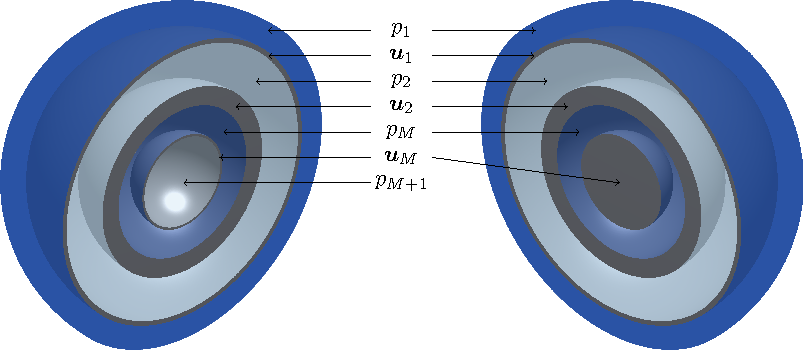
\includegraphics{../../LaTeX/createFigures/TikzFigures/article_e3Dss_PhD/function_distribution}
%	\includegraphics[scale=1]{\graphicsFolder/Figure3}
	\caption{Illustration (clip view) of a model (to the left) with 3 steel shells and a model (to the right) with 2 steel shells surrounding a solid steel sphere, illustrating the distribution of functions (in the case $M=3$). The model to the left models a fluid as the innermost domain, while the model to the right models a solid domain as the innermost domain (note that the expression $\vec{u}_M$ is slightly altered in this case).}
	\label{Fig1:function_distribution}
\end{figure}
Recall that $\hankel_n^{(i)}$, $Z_{j,n}^{(i)}$, $S_{j,n}^{(i)}$ and $T_{j,n}^{(i)}$ are all derived from spherical Bessel functions ($\besselj_n$ and $\bessely_n$), while $Q_n^{(i)}$ are derived from Legendre functions. All coefficients ($A_{m,n}^{(i)}$, $B_{m,n}^{(i)}$ and $C_{m,n}^{(i)}$) are found by solving the linear system of equations in \Cref{Eq1:SystemOfEquations}. The scattered pressure field in the outermost (unbounded) fluid domain, the $m^{\mathrm{th}}$ fluid layer (for $2\leq m \leq M$), and the innermost fluid domain (if present), are given by
\begin{align}\label{Eq1:Summary_p1}
p_1(r,\vartheta) &= \sum_{n=0}^\infty Q_n^{(0)}(\vartheta) C_{1,n}^{(1)} \hankel^{(1)}_n(k_1 r)\\\label{Eq1:Summary_pm}
p_m(r,\vartheta) &= \sum_{n=0}^\infty Q_n^{(0)}(\vartheta)C_{m,n}^{(i)} Z_n^{(i)}(k_m r)\\
	p_{M+1}(r,\vartheta) &= \sum_{n=0}^\infty Q_n^{(0)}(\vartheta) C_{M+1,n}^{(1)} \besselj_n(k_{M+1} r),\label{Eq1:Summary_pM1}
\end{align}
respectively. The displacement field in the $m^{\mathrm{th}}$ solid domain is given by
\begin{equation}
	\vec{u}_m = u_{\mathrm{r},m} \vec{e}_{\mathrm{r}} + u_{\upvartheta,m} \vec{e}_\upvartheta\label{Eq1:Summary_u}
\end{equation}
where
\begin{align}
	u_{\mathrm{r},m}(r,\vartheta) &= \frac{1}{r}\sum_{n=0}^\infty Q_n^{(0)}(\vartheta)\left[A_{m,n}^{(i)}S_{1,n}^{(i)}(a_m r)+B_{m,n}^{(i)}T_{1,n}^{(i)}(b_m r)\right]\\
	u_{\upvartheta,m}(r,\vartheta) &= \frac{1}{r}\sum_{n=0}^\infty Q_n^{(1)}(\vartheta)\left[A_{m,n}^{(i)}S_{2,n}^{(i)}(a_m r)+B_{m,n}^{(i)}T_{2,n}^{(i)}(b_m r)\right].
\end{align} 
If the inner domain is a solid domain, the terms involving $S_{1,n}^{(2)}$ and $T_{1,n}^{(2)}$ in $\vec{u}_M$, are not present.
%%\clearpage
\section{Computational aspects}
\label{Sec1:computationalAspects}
Several computational issues arise when implementing the exact solution (which has been implemented in \href{mathworks.com}{\MATLAB}). The source code can be downloaded from GitHub at \href{https://github.com/Zetison/e3Dss}{https://github.com/Zetison/e3Dss}. In this section, a discussion of some of these issues will be presented.

\subsection{Matrix manipulations}
Note that the only complex valued matrix entries of $\vec{H}_n$ are the first two entries in the first column. So instead of using a complex matrix solution routine to solve the system, one can exploit this fact to solving a real valued linear system of equations with two right hand sides. Refer to Fender~\cite[pp. 18-20]{Fender1972sfa} for details. Moreover, Fender shows that some further matrix manipulation may reduce the overall computational time by 30\% (when doing a frequency sweep). By using the same ideas, the size of $\vec{H}_n$ can be reduced from $6M$ to $4M$.

Note that for $n>0$, column number $2l$, $l=1, 2, \dots, 3M$, of $\vec{H}_n$ contains entries which are linear combinations of $\besselj_n$ and $\besselj_{n+1}$ (and no spherical Bessel functions of second kind), while column number $2l-1$, $l=1, 2, \dots, 3M$, of $\vec{H}_n$ contains entries which are linear combinations of $\bessely_n$ and $\bessely_{n+1}$. So since
\begin{equation}
	\lim_{n\to\infty} |\besselj_n(\zeta)| = 0\quad\text{and}\quad \lim_{n\to\infty} |\bessely_n(\zeta)| = \infty,
\end{equation}
(which is illustrated in \Cref{Fig1:besselPlotLargeN})
\begin{figure}
	\centering
	\begin{subfigure}[t]{0.48\textwidth}
		\centering
		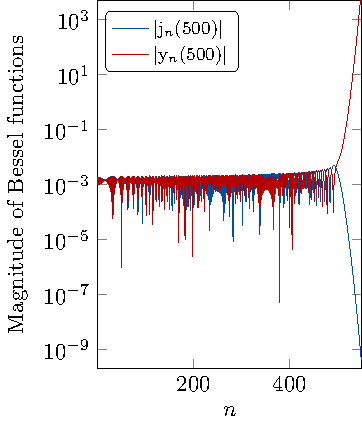
\includegraphics{besselPlotLargeN_1}
		\caption{Magnitude of Besselfunctions ploted for ${n\in[0,550]}$.}
	\end{subfigure}
	~
	\begin{subfigure}[t]{0.48\textwidth}
		\centering
		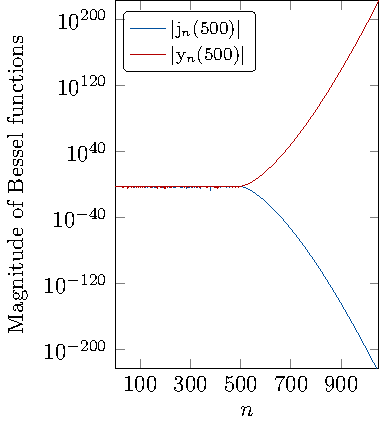
\includegraphics{besselPlotLargeN_2}
		\caption{Magnitude of Besselfunctions ploted for $n\in[0,1050]$.}
	\end{subfigure}
	\caption{Illustration of the asymptotic behavior, of the spherical Bessel functions of first ($\besselj_n(x)$) and second ($\bessely_n(x)$) kind, as a function of $n$, for a fixed argument $x=500$.}
	\label{Fig1:besselPlotLargeN}
\end{figure}
the matrix $\vec{H}_n$ becomes poorly scaled for large $n$. This issue can be solved by scaling the matrix with a (diagonal) preconditioning matrix $\vec{P}_n$ where the diagonal entries are given by the maximal modulus of the corresponding column vectors of $\vec{H}_n$. Defining the vector $\tilde{\vec{C}}_n = \vec{P}_n\vec{C}_n$ and solving the system $\tilde{\vec{H}}_n\tilde{\vec{C}}_n = \vec{D}_n$ with $\tilde{\vec{H}}_n = \vec{H}_n \vec{P}_n^{-1}$, the solution is obtained by $\vec{C}_n = \vec{P}_n^{-1}\tilde{\vec{C}}_n$. In \Cref{Fig1:Spy2K,Fig1:Spy2K2} the magnitude of the entries in $\vec{H}_n$ is visualized before and after preconditioning, respectively.
\begin{figure}
	\centering
	\begin{subfigure}{\textwidth}
		\centering
		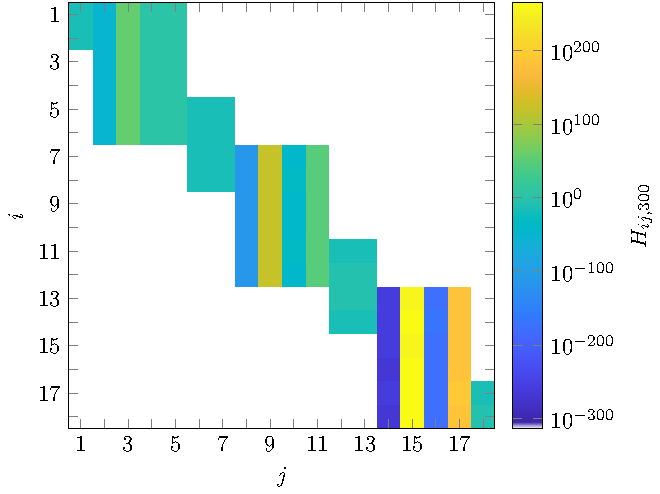
\includegraphics[scale=1]{Spy_K_1}
		\caption{Before preconditioning.}
		\label{Fig1:Spy2K}
	\end{subfigure}
	\par\bigskip
	\begin{subfigure}{\textwidth}
		\centering
		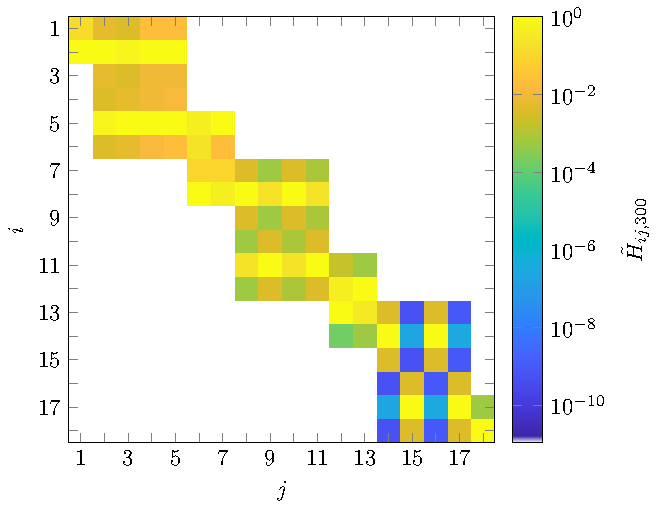
\includegraphics{Spy_K_2}
		\caption{After preconditioning.}
		\label{Fig1:Spy2K2}
	\end{subfigure}
	\caption{\textbf{Matrix manipulations}: Plot of the magnitude of the matrix entries of $\vec{H}_{300}$ and $\tilde{\vec{H}}_{300}$.}
	\label{Fig1:SpyK}
\end{figure}
This example is the matrix $\vec{H}_{300}$ of the S135 benchmark problem (described in \Cref{Subsec1:benchmarkProblem}) at $f=\SI{30}{kHz}$. The condition number was improved from $\operatorname{cond}(\vec{H}_{300}) \approx 7.4\cdot 10^{278}$ to $\operatorname{cond}(\tilde{\vec{H}}_{300}) \approx 9.4\cdot 10^4$.

\subsection{Series evaluation}
\label{Subsec1:seriesEval}
As the series involves summation over infinitely many terms, the series needs to be truncated at some number $n=N_\varepsilon$. Denote by $p_1^{(N)}$, the truncated sum for the scattered pressure in the outer domain (\Cref{Eq1:Summary_pm}), 
\begin{align}\label{Eq1:truncated_p1}
p_1^{(N)}(r,\vartheta) &= \sum_{n=0}^N Q_n^{(0)}(\vartheta) C_{1,n}^{(1)} \hankel^{(1)}_n(k_1 r),
\end{align}
and correspondingly for the other fields in \Cref{Eq1:Summary_pm,Eq1:Summary_pM1,Eq1:Summary_u}.
In~\cite[pp. 32-35]{Ihlenburg1998fea}, Ihlenburg discusses such a value based on the decay of Bessel functions, in which he suggests using $N\approx 2kr$. In this work, however, the summation is terminated whenever the magnitude of term $n=N_\varepsilon$ divided by the magnitude of the partial sum (based on the first $N_\varepsilon+1$ terms) is less than some prescribed tolerance $\varepsilon$. Typically machine epsilon is used for this number, i.e. $\varepsilon \approx 2.220446\cdot 10^{-16}$. As with the suggestion of Ihlenburg, the number of terms, $N_\varepsilon$, grows linearly with the frequency. The computational complexity of the problem is thus $\bigoh(\omega)$. 

The solution is often needed at several points, or frequencies (or a combination of both). In this case, one should compute the solutions at all points at once, such that the calls to the implemented Bessel functions are minimized.

\subsection{Round-off errors}
\label{Subsec1:RoundoffErrors}
Although the products $A_{m,n}^{(2)}S_{j,n}^{(2)}(\zeta)$, $B_{m,n}^{(2)}T_{j,n}^{(2)}(\zeta)$ and $C_{m,n}^{(2)}Z_n^{(2)}(\eta)$ all goes to zero as $n\to\infty$, the functions $S_{j,n}^{(2)}(a_m r)$, $T_{j,n}^{(2)}(\zeta)$ and $Z_n^{(2)}(\eta)$ does not. In fact, these functions become unbounded when $n\to\infty$ because they are all superposition of Bessel functions of second kind with this property. So, since the floating point number has an upper bound\footnote{For double precision this is typically $V_{\mathrm{max}} \approx 1.797693134862316\cdot 10^{308}$.}, there is a limit to the number of terms that can be used. 

A naive solution to this problem is to try higher precision, which can easily be done with MATLAB symbolic class. This, however, increases the computational time drastically. 

In \Cref{Fig1:errorsS123_ASI-6NN} several round-off phenomena which typically arises are illustrated.
\begin{figure}
	\centering
	\begin{subfigure}[t]{0.49\textwidth}
		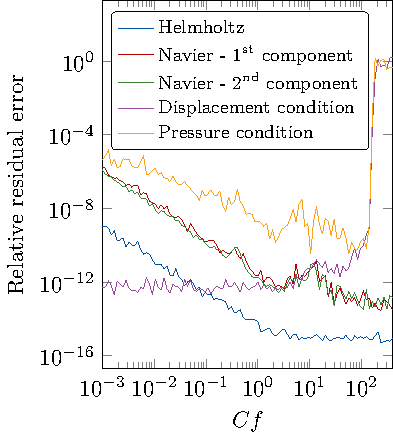
\includegraphics[width=\textwidth]{errors_S135_SSBC_1}
		\caption{Double precision, $\varepsilon \approx 10^{-16}$}
	\end{subfigure}%
	\hspace*{0.02\textwidth}%
	\begin{subfigure}[t]{0.49\textwidth}
		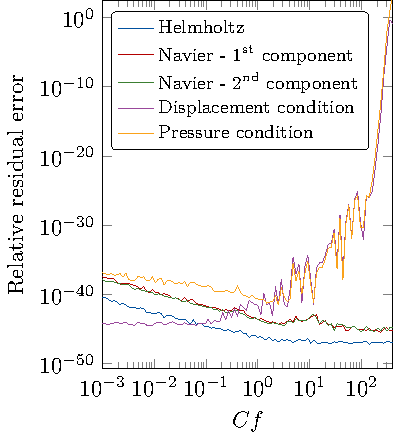
\includegraphics[width=\textwidth]{errors_S135_SSBC_2}
		\caption{Symbolic precision $\varepsilon \approx 10^{-40}$}
	\end{subfigure}
	\caption{\textbf{Round-off errors}: Residual errors for the governing equations and boundary conditions. The use of symbolic precision in MATLAB illustrate that the errors are due to round-off errors. The relative residual formulas for the Helmholtz equation, the first and second components of the Navier equation, the displacement condition and the pressure conditions are given by \Cref{Eq1:residualHelmhotlz,Eq1:residualNavier1,Eq1:residualNavier2,Eq1:residualDisplacement,Eq1:residualPressure}, respectively.}
	\label{Fig1:errorsS123_ASI-6NN}
\end{figure}
The specific example used here is the S135 benchmark problem with SSBC (described in \Cref{Subsec1:benchmarkProblem}). The incident wave, $p_{\mathrm{inc}}$, is a plane wave traveling in the direction given by $\vartheta=\ang{60}$ and $\varphi=\ang{240}$ (see \Cref{Sec1:resultsDisc}). An uniform (relative to the spherical coordinate system) set of sample points are distributed in all domains\footnote{It is placed 32 points in each domain except for the inner domain with 25 points. The distribution of point in the radial direction in the exterior domain is limited to the interval $[R_{0,1}, 2R_{0,1}]$.} where the residual error in the Helmholtz equation (\Cref{Eq1:helmholtz}), the $1^{\mathrm{st}}$ and $2^{\mathrm{nd}}$ component of Navier's equation in spherical coordinates (\Cref{Eq1:navierSphericalSimplified1,Eq1:navierSphericalSimplified2}, respectively), the displacement condition (\Cref{Eq1:firstBC}) and the pressure condition (\Cref{Eq1:secondBC}), is measured. By using the infinity norm, $\|\cdot\|_\infty$, for each residual, and dividing by the magnitude of the terms involved, the relative residual error is obtained. The maximal relative residual in all domains can then be calculated. In particular, these relative residual errors are given by
\begin{align}%
	&\max_{1\leq m\leq M+1}\frac{\left\|\left(\nabla^2 + k_m^2\right)p_m\right\|_\infty}{\left\|k_m^2p_m\right\|_\infty}\label{Eq1:residualHelmhotlz}\\
	&\resizebox{0.9\textwidth}{!}{$\displaystyle\max_{1\leq m\leq M}\frac{\left\|\pderiv{\sigma_{\mathrm{rr},m}}{r} + \frac{1}{r}\pderiv{\sigma_{\mathrm{r}\upvartheta,m}}{\vartheta} + \frac{1}{r}\left(2\sigma_{\mathrm{r}\mathrm{r},m} - \sigma_{\upvartheta\upvartheta,m} - \sigma_{\upvarphi\upvarphi,m} + \sigma_{\mathrm{r}\upvartheta,m}\cot\vartheta\right) + \omega^2\rho_{\mathrm{s},m}u_{\mathrm{r},m}\right\|_\infty}{\left\|\omega^2\rho_{\mathrm{s},m}u_{\mathrm{r},m}\right\|_\infty}$}\label{Eq1:residualNavier1}\\
	&\resizebox{0.9\textwidth}{!}{$\displaystyle\max_{1\leq m\leq M}\frac{\left\|\pderiv{\sigma_{\mathrm{r}\upvartheta,m}}{r} + \frac{1}{r}\pderiv{\sigma_{\upvartheta\upvartheta,m}}{\vartheta} + \frac{1}{r}\left[(\sigma_{\upvartheta\upvartheta,m} - \sigma_{\upvarphi\upvarphi,m})\cot\vartheta + 3\sigma_{\mathrm{r}\upvartheta,m} \right] +\omega^2\rho_{\mathrm{s},m}u_{\upvartheta,m}\right\|_\infty}{\left\|\omega^2\rho_{\mathrm{s},m}u_{\upvartheta,m}\right\|_\infty}\label{Eq1:residualNavier2}$}\\
	&\max_{1\leq m\leq M}\frac{\left\|\rho_{\mathrm{f}} \omega^2 u_{\mathrm{r}} - \pderiv{p_{\mathrm{tot}}}{r}\right\|_\infty}{\left\|\pderiv{p_{\mathrm{tot}}}{r}\right\|_\infty}\label{Eq1:residualDisplacement}\\
	&\max_{1\leq m\leq M}\frac{\left\|\sigma_{\mathrm{rr}} + p_{\mathrm{tot}}\right\|_\infty}{\left\|p_{\mathrm{tot}}\right\|_\infty}.\label{Eq1:residualPressure}%$}
\end{align}
By comparing these error results for both double precision and symbolic precision in MATLAB, one can conclude that the errors indeed originate from round-off errors. When using double precision, the summation is ended whenever $|\bessely_n(\eta)| > 10^{290}$, such that invalid solutions is obtained for sufficiently large $n$. Since one needs to have enough terms for the solution to converge, and at the same time have to avoid computing $\bessely_n(\eta)$ for low $\eta$ (and large $n$), the following bound on the frequency based on experimental data is suggested
\begin{equation}\label{Eq1:Upsilon}
	f \lesssim \frac{100}{C},\qquad C =\left(\frac{R_{0,1}}{c_{\mathrm{f},1}}\right)^{\frac{3}{2}}\frac{1}{\sqrt{\Upsilon}}
\end{equation}
with
\begin{equation*}
	\Upsilon = \min\left\{\min_{1\leq m\leq M}\frac{R_{1,m}}{\max\{c_{\mathrm{s,1},m},c_{\mathrm{s,2},m}\}},\min_{1\leq m\leq M}\frac{R_{0,m}}{c_{\mathrm{f},m}}\right\}
\end{equation*}
where $c_{\mathrm{s,1},M}$ and $c_{\mathrm{s,2},M}$ is the transverse and longitudinal wave velocity for the $M^{\mathrm{th}}$ spherical shell, respectively. The constant $\Upsilon$ corresponds to the lowest argument $\eta$ used for the Bessel functions of second kind. An addendum will be given to yield more numerical evidence for this bound. In particular, plots similar to the ones in \Cref{Fig1:errorsS123_ASI-6NN} will be presented for all benchmarks and corresponding boundary conditions in \Cref{Subsec1:benchmarkProblem}. However, it would certainly be possible to construct models in which this bound is not valid.

One can also observe significant round-off errors for very low frequencies which is again due to the evaluation of the spherical Bessel functions of the second kind with the property
\begin{equation}
	\lim_{\zeta\to 0} |\bessely_n(\zeta)| = \infty.
\end{equation}
Finally, observe that problems for higher frequencies also occur when using the symbolic class in MATLAB (even though the summation is not terminated prematurely), which calls for a more mathematically sound way of solving this issue. To avoid evaluating the Bessel functions directly, one could include a scaling such that one need to evaluate products of the form $\besselj_n(\xi)\bessely_n(\eta)$, $\besselj_{n+1}(\xi)\bessely_n(\eta)$, $\besselj_n(\xi)\bessely_{n+1}(\eta)$ and $\besselj_{n+1}(\xi)\bessely_{n+1}(\eta)$ (which will be $0\cdot\infty$ type products). One would then probably need to use relations like~\cite[\href{http://functions.wolfram.com/03.21.26.0047.01}{03.21.26.0047.01} and \href{http://functions.wolfram.com/03.21.26.0049.01}{03.21.26.0049.01}]{WolframResearch2016m}
\begin{align}
\besselj_n(\sqrt{z})\bessely_n(\sqrt{z}) &=-\frac{\sqrt{\PI}}{2}G_{1,3}^{2,0}\left(z\Bigg\vert\begin{matrix}
	0\\
	-\frac{1}{2}, n, -n-1
	\end{matrix}\right)\\
	\besselj_{n+1}(\sqrt{z})\bessely_n(\sqrt{z}) &=\frac{\sqrt{\PI}}{2}G_{2,4}^{2,1}\left(z\Bigg\vert\begin{matrix}
	0,-\frac{1}{2}\\
	0, n+\frac{1}{2},-1,-n-\frac{3}{2}
	\end{matrix}\right)
\end{align}
where $G$ is the Meijer G-function. This investigation is left as future work.






%%\clearpage
\section{Numerical examples} 
\label{Sec2:resultsDisc}
Rigid scattering on a sphere and elastic scattering on a spherical shell are investigated in the following. These problems possess analytic solutions~\cite{Venas2019e3s} and are for this reason often used to verify numerical methods in acoustic scattering, e.g.~\cite{Gerdes1996so3,Ihlenburg1998fea,Simpson2014aib,Gerdes1998tcv,Gerdes1999otp,Coox2017aii}.  

The mock shell is analyzed to investigate the infinite element formulations, and we end this section by analyzing a simplified submarine benchmark.

In this work, the test setting is chosen so that the present approach can be compared to other methods. In particular, the scattering on a rigid sphere example found in~\cite{Simpson2014aib} and the scattering on a spherical shell used in~\cite{Ihlenburg1998fea} are addressed. The latter problem will be investigated in depth and we shall build upon this problem to include both rigid scattering and scattering with full ASI on both sides of the shell.

The direction of the incident wave is along the $x$-axis while the symmetry of the parametrization of the domain is around the $z$-axis (to avoid exploitation of the symmetry of the problems).

We define the \textit{SAV index} by
\begin{equation}
	I_{\mathrm{SAV}} = \frac{L_{\Gamma_{\mathrm{a}}}}{2}\frac{|\Gamma_0|}{|\Omega_{\mathrm{a}}|}
\end{equation}
where $L_{\Gamma_{\mathrm{a}}}$ is the characteristic length of the artificial boundary, $|\Gamma_0|$ is the surface area of the scatterer and $|\Omega_{\mathrm{a}}|$ is the volume of the discretized fluid between $\Gamma_0$ and $\Gamma_{\mathrm{a}}$. The SAV index is based on a scaled surface-area-to-volume ratio (SA/V) such that the domain of computation is fitted in a unit sphere. It can be thought of as an efficiency index for the IEM compared to BEM, as problems with low $I_{\mathrm{SAV}}$ will be more suited for BEM, while high values of $I_{\mathrm{SAV}}$ will be more suited for IEM. If we for the sphere example place the artificial boundary, $\Gamma_{\mathrm{a}}$, at $r_{\mathrm{a}}=sR_0$, where $R_0$ is the outer radius of the scatterer, then the SAV index is given by
\begin{equation}
	I_{\mathrm{SAV}} = \frac{3s}{s^3-1}.
\end{equation}
The IEM is optimal for the sphere problem in the sense that the SAV index can be arbitrarily large. In fact, the infinite elements can be attached directly onto the scatterer (such that ${I_{\mathrm{SAV}}=\infty}$) as done in~\cite{Shirron2002aie}. This, however, is not the case for more complex geometries. 

A typical SAV index for submarines like the one depicted in \Cref{Fig2:model3_in_waterInf} is approximately~5, so by choosing $s>1$, the SAV index can be adjusted for a fairer comparison with methods like BEM. In the numerical experiments on spherical shells we use $s=\frac{32+\PI}{32-\PI}\approx 1.2$ (such that the aspect ratio of the elements in the tensor product meshes are minimal), resulting in $I_{\mathrm{SAV}}\approx 4.5$.
\begin{figure}
	\centering
	\begin{subfigure}{0.3\textwidth}
		\centering
		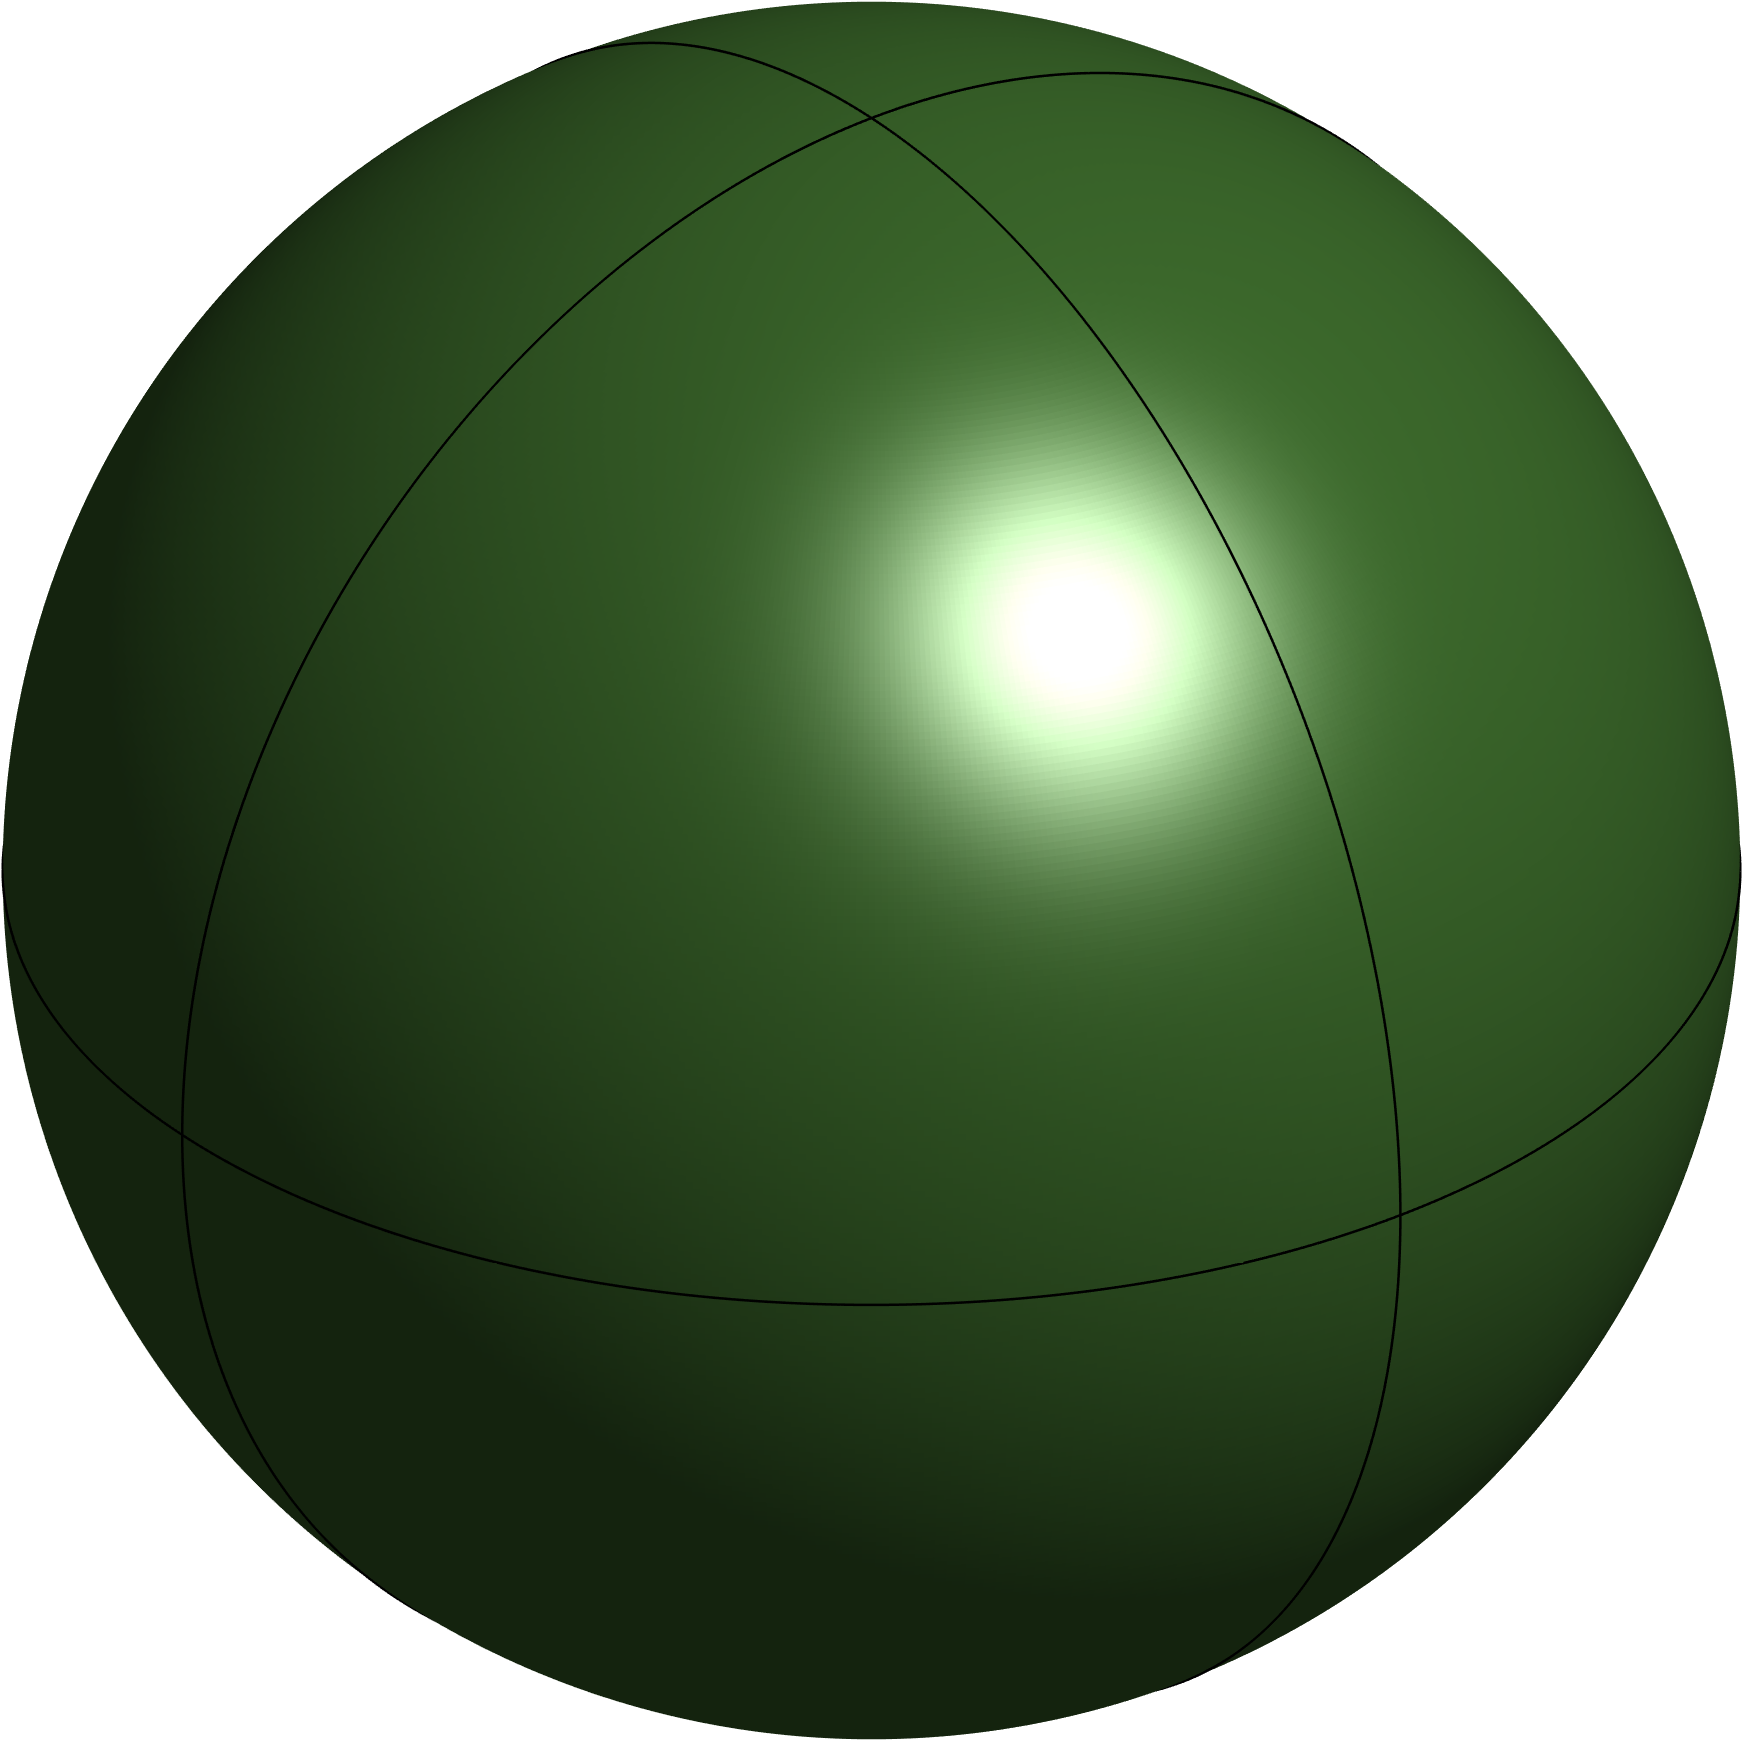
\includegraphics[width=0.8\textwidth]{sphericalShellMesh1_2_0}
		\caption{Mesh ${\cal M}_{1,\check{p},\check{k}}^{\textsc{iga}}$}
		\label{Fig2:SphericalShellMeshes1}
    \end{subfigure}
    ~
	\begin{subfigure}{0.3\textwidth}
		\centering
		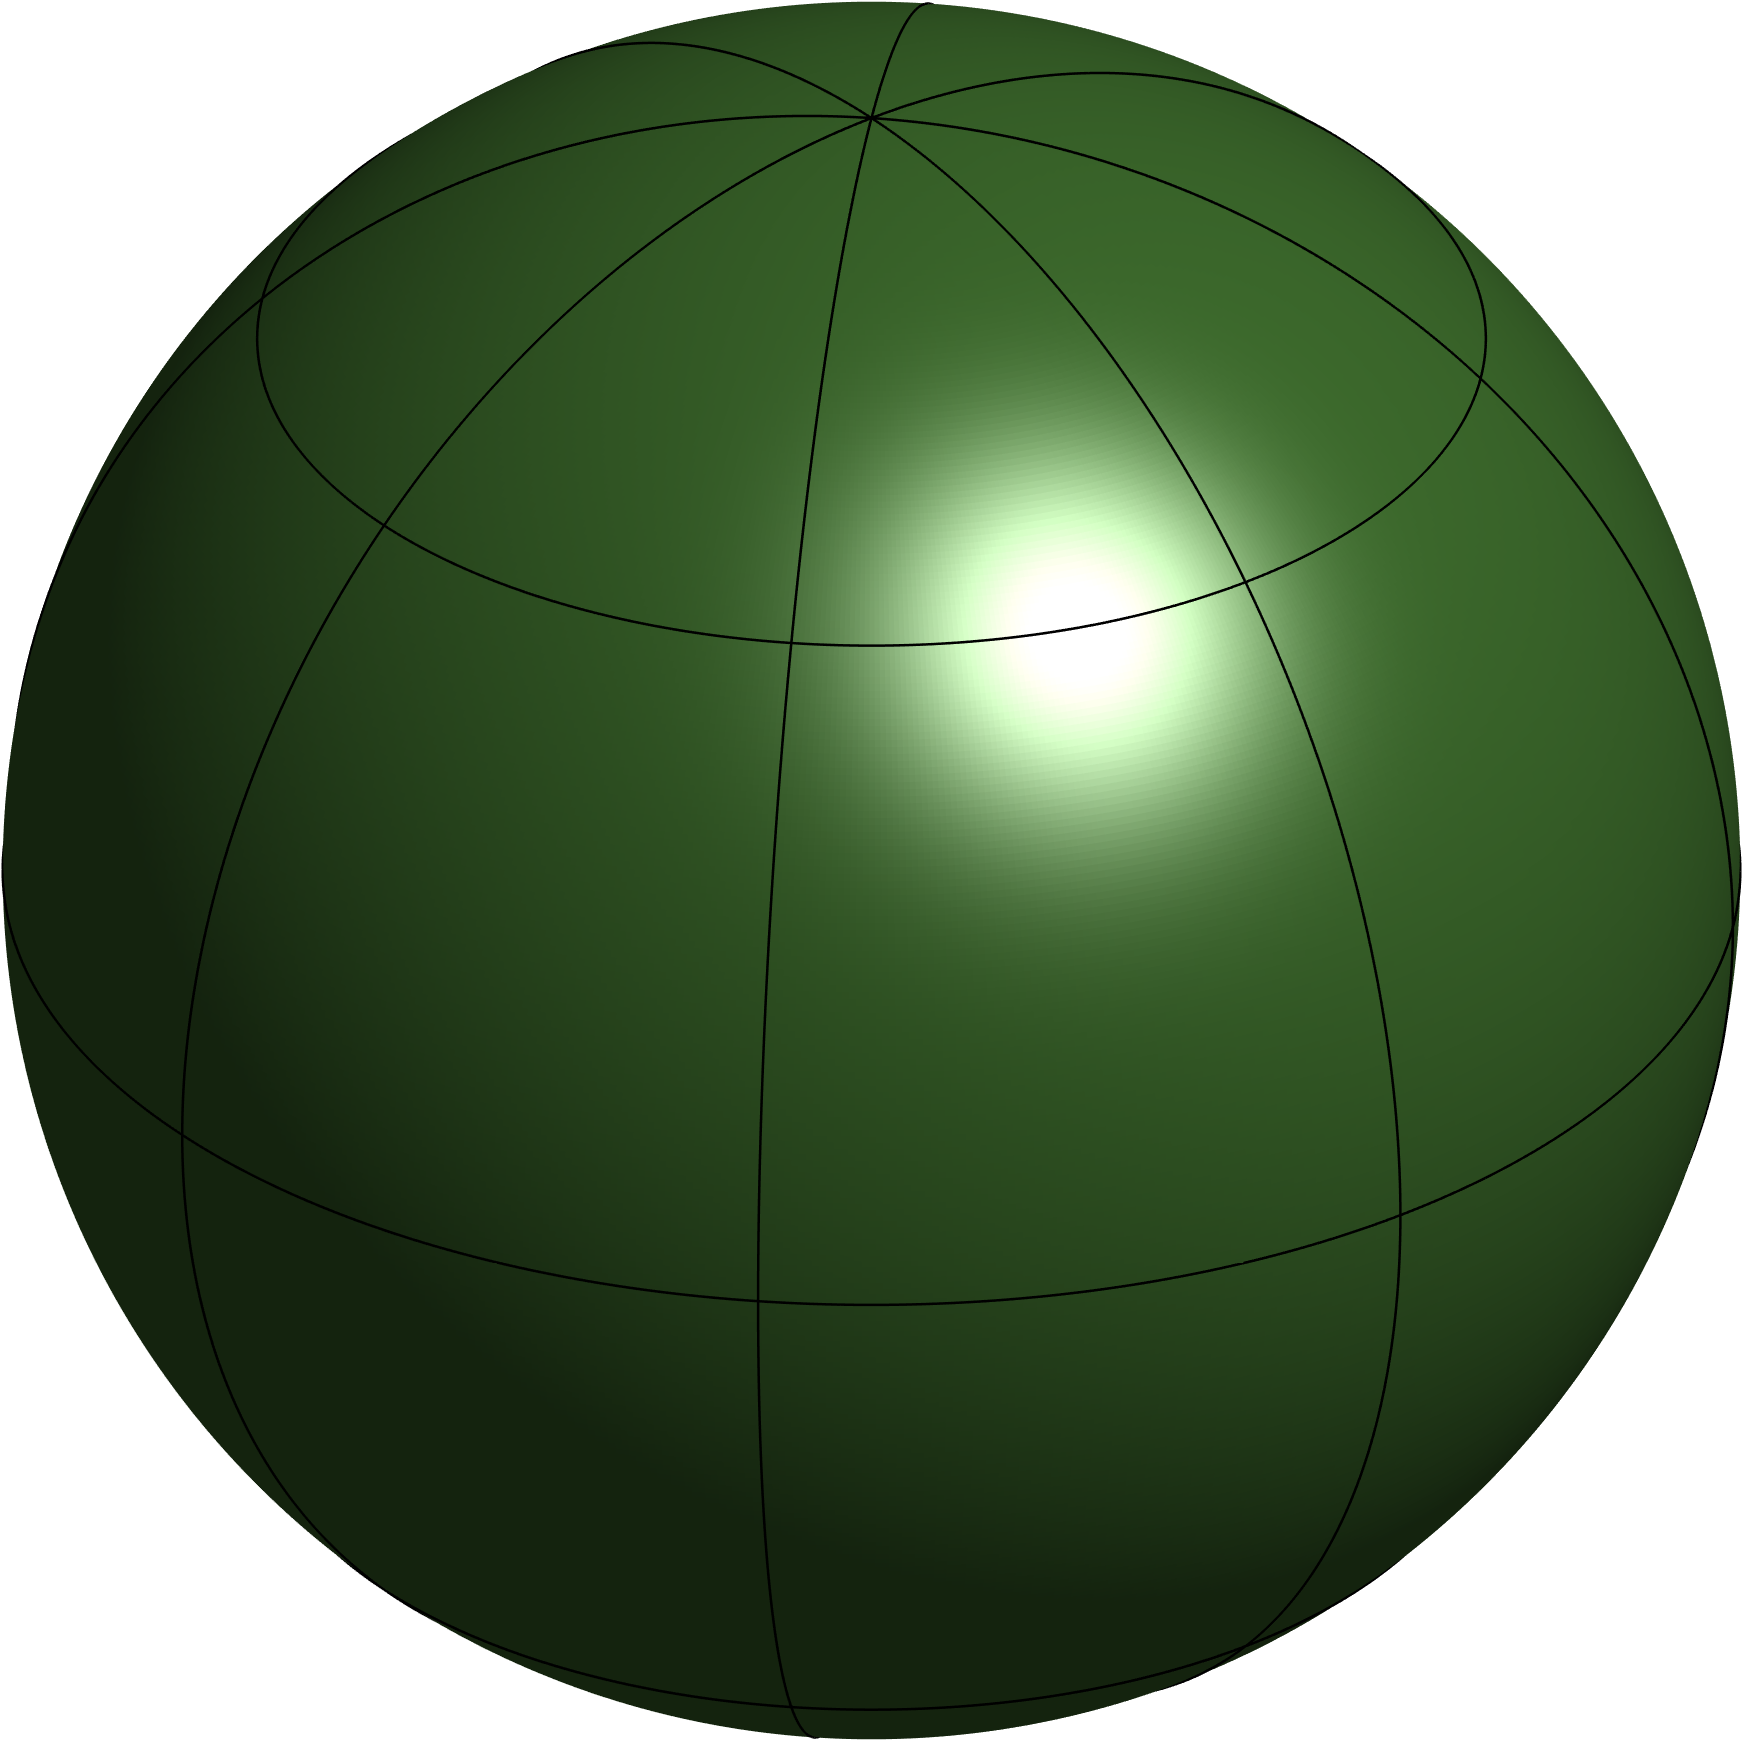
\includegraphics[width=0.8\textwidth]{sphericalShellMesh2_2_0}
		\caption{Mesh ${\cal M}_{2,\check{p},\check{k}}^{\textsc{iga}}$}
		\label{Fig2:SphericalShellMeshes2}
    \end{subfigure}
    ~
	\begin{subfigure}{0.3\textwidth}
		\centering
		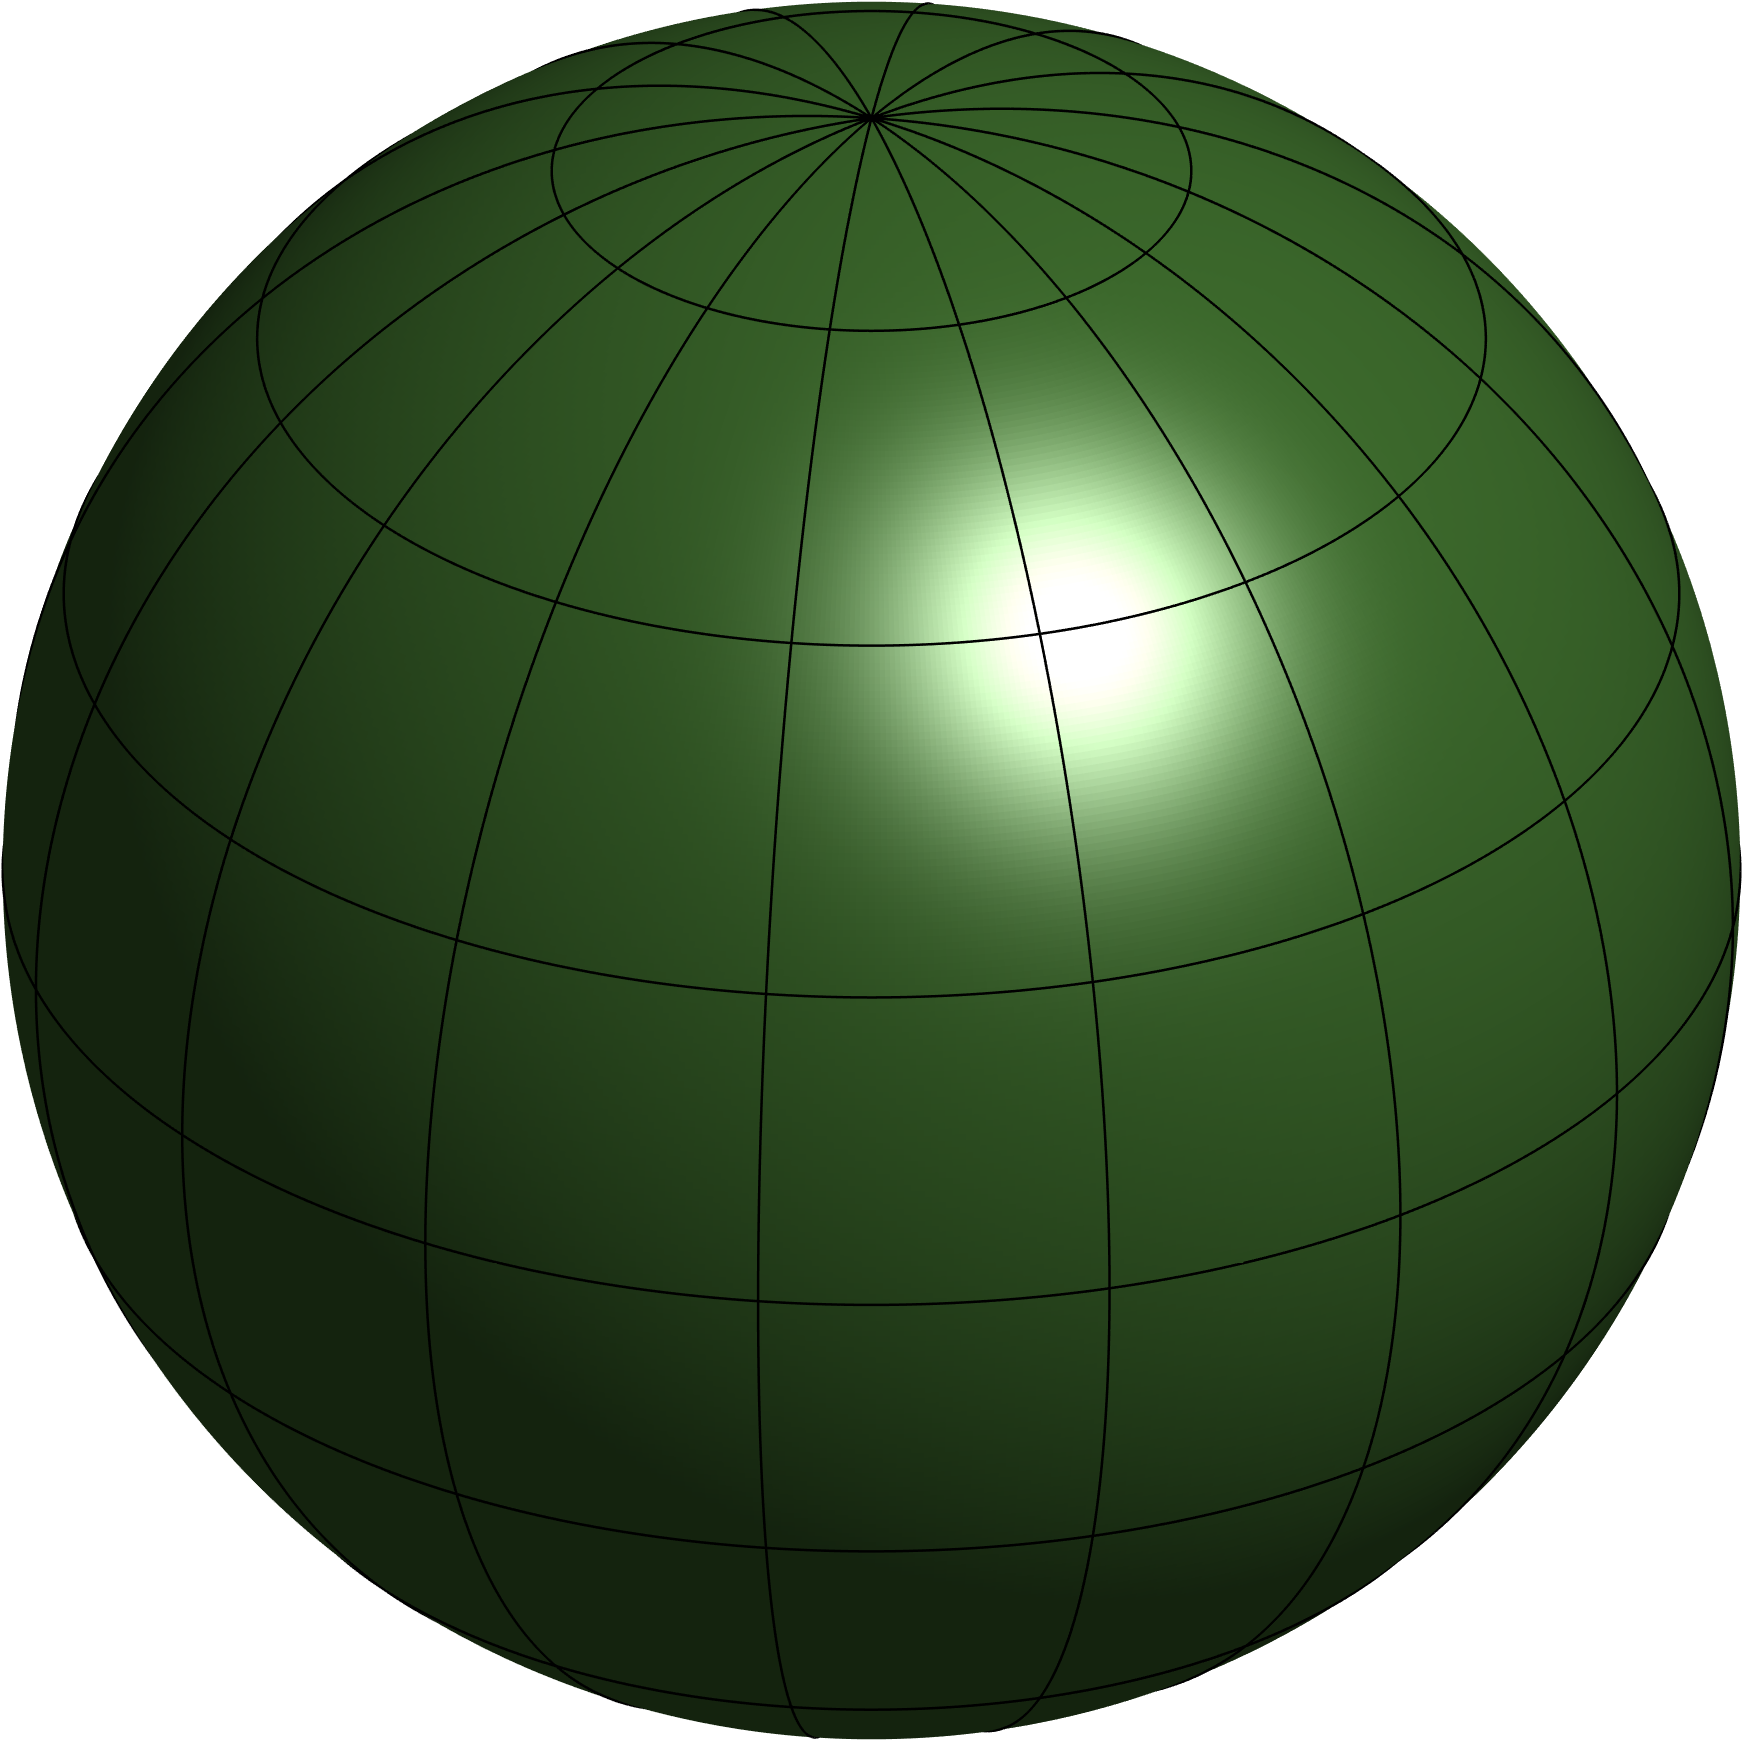
\includegraphics[width=0.8\textwidth]{sphericalShellMesh3_2_0}
		\caption{Mesh ${\cal M}_{3,\check{p},\check{k}}^{\textsc{iga}}$}
		\label{Fig2:SphericalShellMeshes3}
    \end{subfigure}
	\caption{\textbf{Numerical examples}: Illustration of the first three meshes, using two successive refinements from the coarse mesh ${\cal M}_{1,\check{p},\check{k}}^{\textsc{iga}}$.}
	\label{Fig2:SphericalShellMeshes}
\end{figure}

The meshes will be generated from a standard discretization of a sphere using NURBS as seen in \Cref{Fig2:SphericalShellMeshes}. We shall denote by ${\cal M}_{m,\check{p},\check{k}}^{\textsc{iga}}$, mesh number $m$ with polynomial order $\check{p}$ and continuity $\check{k}$ across element boundaries\footnote{Except for some possible $C^0$ lines in the initial CAD geometry.}. For the corresponding FEM meshes we denote by ${\cal M}_{m,\check{p},\mathrm{s}}^{\textsc{fem}}$ and ${\cal M}_{m,\check{p},\mathrm{i}}^{\textsc{fem}}$ the subparametric and isoparametric FEM meshes, respectively. The construction of NURBS meshes are illustrated in \Cref{Fig2:SphericalShellMeshes}. The initial mesh is depicted as mesh ${\cal M}_{1,\check{p},\check{k}}^{\textsc{iga}}$ in \Cref{Fig2:SphericalShellMeshes1} and is refined only in the angular directions for the first 3 refinements (that is, mesh ${\cal M}_{4,\check{p},\check{k}}^{\textsc{iga}}$ only have one element thickness in the radial direction). Mesh ${\cal M}_{m,\check{p},\check{k}}^{\textsc{iga}}$, $m=5,6,7$, have 2, 4 and 8 elements in its thickness, respectively. This is done to obtain low aspect ratios for the elements. All the meshes will then be nested and the refinements are done uniformly. We shall use the same polynomial order in all parameter directions; $\check{p}_\upxi=\check{p}_\upeta=\check{p}_\upzeta$. 

Unless otherwise stated, we shall use the BGU formulation and $N=4$ basis functions in the radial direction of the infinite elements.

\subsection{Simpson benchmark}
The configuration presented by Simpson et al.~\cite{Simpson2014aib} is considered: a rigid sphere of radius $R_0=\SI{0.5}{m}$ is impinged by an incident plane wave and the total pressure is measured at a distance $r=\SI{5}{m}$ from the origin. 

This is a low frequency problem with $k=\SI{2}{m^{-1}}$. It is emphasized that the trace of the NURBS discretization of the domain $\Omega_{\mathrm{a}}$ at the surface $\Gamma_0$ reduces to the exact same NURBS discretization used in~\cite{Simpson2014aib} to discretize the boundary $\Gamma_0$. 

From \Cref{Fig2:simpsonPlot} we observe that the IGA infinite element method (IGAIE) exploits the available degrees of freedom at $\Gamma_0$ more effectively than the IGA boundary element method (IGABEM) in~\cite{Simpson2014aib}\footnote{Due to low resolution of the plots in~\cite[Fig. 17]{Simpson2014aib}, the results were reproduced and sampled at 3601 points (rather than 30 points) using our own IGABEM implementation.}. 

By projecting the analytic solution onto this set of NURBS basis functions at $\Gamma_0$ (the best approximation in the $L_2$-norm by least squares projection, IGA best approximation, IGABA), it is revealed that even more accuracy can potentially be made. This is an inherent problem for Galerkin FEM when solving the Helmholtz equation and is related to the pollution effect \cite{Babuska1995agf}. All IEM formulations (PGU, PGC, BGU and BGC) gave approximately the same result in this case.
\begin{figure}
	\centering
	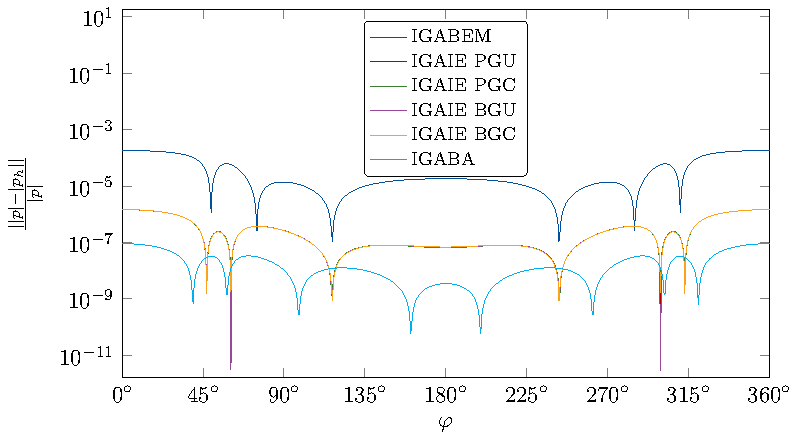
\includegraphics[width=\textwidth]{simpson}
	\caption{\textbf{Simpson benchmark}: The relative error in the modulus of the pressure is plotted on a circle (azimuth direction, $\varphi$) in the $xy$-plane at $r=\SI{5}{m}$. All simulations were computed on mesh ${\cal M}_{3,3,2}^{\textsc{iga}}$. The IGAIE formulations here produce roughly the same result.}
	\label{Fig2:simpsonPlot}
\end{figure}

\subsection{Ihlenburg benchmark}
Three benchmark solutions based on the model problem after Ihlenburg~\cite[p. 191]{Ihlenburg1998fea} with parameters given in \Cref{Tab2:IhlenburgParameters}, are investigated. 
\begin{table}
	\centering
	\caption{\textbf{Ihlenburg benchmark}: Parameters for the Ihlenburg benchmark problems.}
	\label{Tab2:IhlenburgParameters}
	\begin{tabular}{l l}
		\toprule
		Parameter & Description\\
		\midrule
		$P_{\mathrm{inc}}=\SI{1}{Pa}$ & Amplitude of incident wave\\
		$E = \SI{2.07e11}{Pa}$ & Young's modulus\\
		$\nu = 0.3$ & Poisson's ratio\\
		$\rho_{\mathrm{s}} = \SI{7669}{kg.m^{-3}}$ & Density of solid\\
		$\rho_{\mathrm{f}} = \SI{1000}{kg.m^{-3}}$ & Density of water\\
		$c_{\mathrm{f}} = \SI{1524}{m.s^{-1}}$ & Speed of sound in water\\
		$R_0=\SI{5.075}{m}$ & Outer radius\\
		$R_1=\SI{4.925}{m}$ & Inner radius\\
		\bottomrule
	\end{tabular}
\end{table}
The parameters for the fluid domains are the speed of sound in water $c_{\mathrm{f}}$ and the fluid density $\rho_{\mathrm{f}}$, and the parameters for the solid domain are the Young's modulus, $E$, the Poisson's ratio $\nu$ and the solid density $\rho_{\mathrm{s}}$. The first benchmark is a simple rigid scattering case (with sound-hard boundary conditions, SHBC) on a sphere with radius $R_0$. The second benchmark problem on a spherical shell has ASI conditions at the outer radius, $R_0$, and homogeneous Neumann condition at the inner radius, $R_1$ (sound-soft boundary conditions, SSBC). This case can be thought of as an approximation of a scattering problem on a spherical shell with an internal fluid with very low density. The third and final benchmark is a further extension with ASI conditions on both sides of the spherical shell (Neumann-Neumann conditions on both surfaces of the shell, NNBC). All of these benchmarks have analytic solutions~\cite{Venas2019e3s} (see \Cref{Fig2:ihlenburgTSexact,Fig2:ihlenburg3Dexact}), which enables computation of the error in the energy norm. As we use the same parameters in both fluids, we denote the common wave number in these fluids by $k=k_1=k_2$.
\begin{figure}
	\centering
	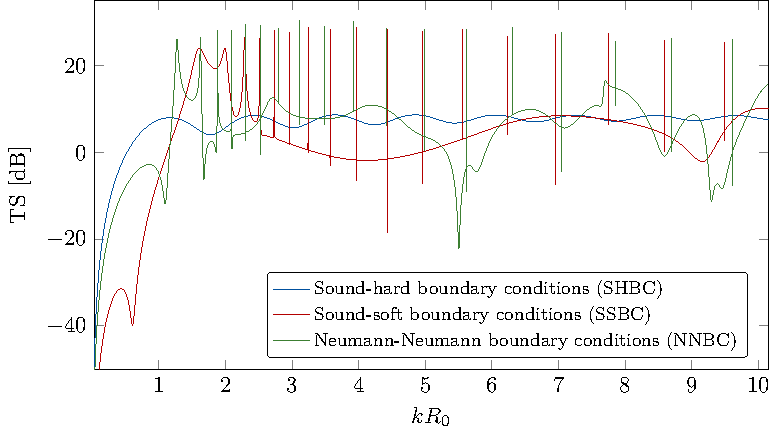
\includegraphics[width=\textwidth]{ihlenburg}
	\caption{\textbf{Ihlenburg benchmark}: Analytic solutions to the scattering problem on a spherical shell with parameters given in \Cref{Tab2:IhlenburgParameters}. The far field pattern of backscattered pressure is plotted against the wave number $k$. A single Neumann condition at the outer radius, $R_0$, corresponds to the rigid scattering case with $\vec{u}=\zerovec$ and $p_2=0$. ASI at $R_0$ and Neumann at $R_1$ models $p_2=0$. Note that Ihlenburg~\cite[p. 192]{Ihlenburg1998fea} plots the far field pattern in \Cref{Eq2:farfield} instead of the target strength, $\TS$, in \Cref{Eq2:TS}.}
	\label{Fig2:ihlenburgTSexact}
\end{figure}
\begin{figure}
	\centering
	\begin{subfigure}[t]{0.48\textwidth}
		\centering
		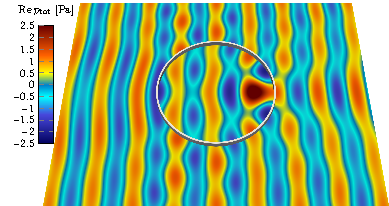
\includegraphics[width=\textwidth]{ihlenburg_nearField_real}
		\caption{Plot of the real part of the total pressure.}
	\end{subfigure}
	~
	\begin{subfigure}[t]{0.48\textwidth}
		\centering
		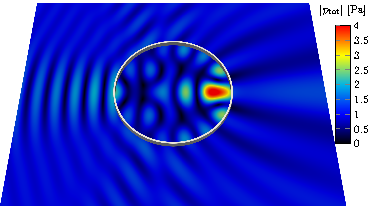
\includegraphics[width=\textwidth]{ihlenburg_nearField_abs}
		\caption{Plot of the modulus of the total pressure.}
	\end{subfigure}
	
	\caption{\textbf{Ihlenburg benchmark with NNBC}: The analytic solution with ASI at both $R_0$ and $R_1$ with $kR_0=10.15$ is plotted in the $xy$-plane. The solid domain is cut open for visualization purposes.}
	\label{Fig2:ihlenburg3Dexact}
\end{figure}
For each experiment, we use the same NURBS order everywhere. Denote by $\check{p}_\upxi = \check{p}_{\upxi,\mathrm{f}} = \check{p}_{\upxi,\mathrm{s}}$ the common NURBS order in the fluid and the solid in the $\xi$-direction. Similarly $\check{p}_\upeta = \check{p}_{\upeta,\mathrm{f}} = \check{p}_{\upeta,\mathrm{s}}$ and $\check{p}_\upzeta = \check{p}_{\upzeta,\mathrm{f}} = \check{p}_{\upzeta,\mathrm{s}}$. Moreover, we denote by $\check{p} = \check{p}_\upxi = \check{p}_\upeta = \check{p}_\upzeta$ the common polynomial orders in all domains.

In order to compare $C^0$ FEM and IGA on the scattering problem, we shall transform the NURBS mesh to a $C^0$ FEM mesh. We use the technique described in \Cref{Sec2:NURBStransformation} to get an isoparametric B-spline approximation of the geometry (isoparametric FEM). This parametrization will have $C^0$ continuity at element boundaries and correspondingly $G^0$ continuity of the geometry representation (i.e. with kinks). The geometric approximation error is of one order higher than the finite element approximation of the solution \cite{Strang1973aao}, so one could expect the $C^0$-IGA meshes (with $\check{k}=0$) to produce the same accuracy as the isoparametric FEM meshes of higher order ($\check{p}\geq 2$). It should be noted that the FEM analysis would then use the Bernstein basis instead of the classical Lagrange basis. However, both of these set of functions spans the same spaces, such that the results should be identical in the absence of round-off errors. 

In \Cref{Fig2:EnergyErrorPlotsDofs} we illustrate $h$-refinement through the error in the energy norm for the first benchmark example (rigid scattering).
\begin{figure}
	\centering
	\includegraphics[width=\textwidth]{L2normPlots_SHBC_dofs}
	\caption{\textbf{Ihlenburg benchmark with SHBC}: Convergence analysis on the rigid scattering case with $k=\SI{1}{m^{-1}}$ and mesh ${\cal M}_m$, $m=1,\dots,7$, using $N=6$. The relative energy error (\Cref{Eq2:energyNormFluids}) is plotted against the degrees of freedom.}
	\label{Fig2:EnergyErrorPlotsDofs}
	\par\bigskip
	\includegraphics[width=\textwidth]{L2normPlots_SHBC_nepw}
	\caption{\textbf{Ihlenburg benchmark with SHBC}: Convergence analysis on the rigid scattering case with $k=\SI{1}{m^{-1}}$ and mesh ${\cal M}_m$, $m=1,\dots,7$, using $N=6$. The relative energy error (\Cref{Eq2:energyNormFluids}) is plotted against the number of elements per wave.}
	\label{Fig2:EnergyErrorPlotsh}
\end{figure}
Predicted convergence rates are not obtained until the aspect ratio of the elements are reduced sufficiently (that is, from mesh ${\cal M}_4$ and onward). By comparing the results of mesh ${\cal M}_{m,2,\mathrm{i}}^{\textsc{fem}}$ and mesh ${\cal M}_{m,2,0}^{\textsc{iga}}$ it can be concluded that the geometry error of mesh ${\cal M}_{m,2,\mathrm{i}}^{\textsc{fem}}$ has almost no impact on the accuracy. However, when using maximum continuity, we get significantly better results. Expected convergence rates are visualized in \Cref{Fig2:EnergyErrorPlotsh} where we now plot the energy norm against $\lambda/h_{\mathrm{max}}$ (corresponding to the number of elements per wave) with $\lambda$ being the wavelength $\lambda=2\pi/k$. A key observation is that the number of elements per wave (needed to obtain a given accuracy) is greatly reduced with higher order IGA methods compared to the classical linear FEM (where 10 elements per wavelength is typically desired for engineering precision, \cite[p. 182]{Ihlenburg1998fea}). The result for the subparametric meshes ${\cal M}_{m,2,\mathrm{s}}^{\textsc{fem}}$ indicates that the convergence rate is reduced due to the reduced accuracy in the geometric representation. This is to be expected as shown in \cite[p. 202]{Strang1973aao}.

\begin{figure}
	\centering
	\begin{subfigure}{0.3\textwidth}
		\centering
		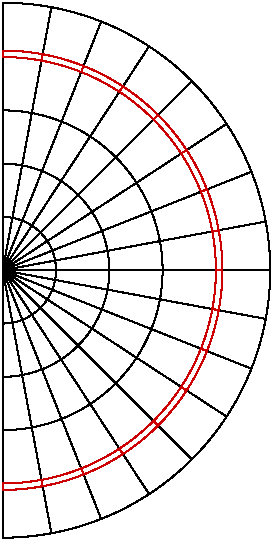
\includegraphics[width=0.6\textwidth]{NNBC_IGAmesh4}
		\caption{Mesh ${\cal M}_{4,\check{p},\check{k}}^{\textsc{iga}}$}
		\label{Fig2:SphericalShellMeshes1NNBC}
    \end{subfigure}
    ~
	\begin{subfigure}{0.3\textwidth}
		\centering
		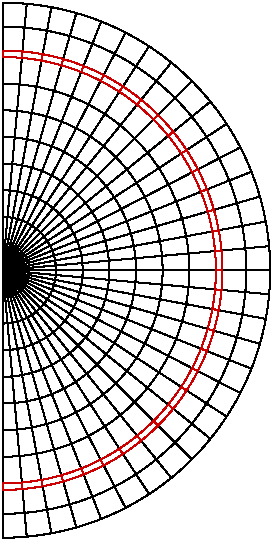
\includegraphics[width=0.6\textwidth]{NNBC_IGAmesh5}
		\caption{Mesh ${\cal M}_{5,\check{p},\check{k}}^{\textsc{iga}}$}
		\label{Fig2:SphericalShellMeshes2NNBC}
    \end{subfigure}
    ~
	\begin{subfigure}{0.3\textwidth}
		\centering
		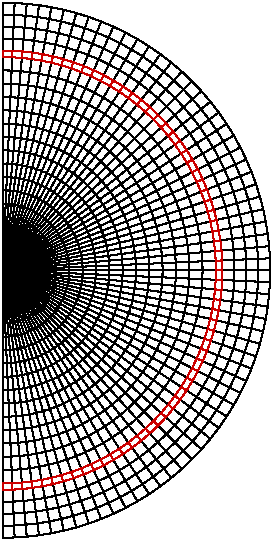
\includegraphics[width=0.6\textwidth]{NNBC_FEMlinear6}
		\caption{Mesh ${\cal M}_{6,1,\mathrm{i}}^{\textsc{fem}}$}
		\label{Fig2:SphericalShellMeshes3NNBC}
    \end{subfigure}
	\caption{\textbf{Ihlenburg benchmark with NNBC}: Illustration of some meshes for the full ASI problem in the $xz$-plane ($x>0$), where the mesh lines for the solid domain is colored red. The full mesh is obtained by rotation around the $z$-axis. Mesh ${\cal M}_{5,2,\mathrm{i}}^{\textsc{fem}}$ is visually indistinguishable from ${\cal M}_{5,\check{p},\check{k}}^{\textsc{iga}}$.}
	\label{Fig2:SphericalShellMeshesNNBC}
\end{figure}
Approaching the ASI problems, we illustrate some meshes in \Cref{Fig2:SphericalShellMeshesNNBC} for the full ASI problem. The corresponding meshes for the SSBC problem (with $p_2=0$) are obtained by removing the mesh inside the solid domain. In \Cref{Fig2:TSPlotSHBC,Fig2:errorPlotSHBC,Fig2:TSPlotSSBC,Fig2:errorPlotSSBC,Fig2:TSPlotNNBC,Fig2:errorPlotNNBC} the target strength, $\TS$, and the error in the energy norm is plotted against the scaled wave number, $kR_0$, in all of the three Ihlenburg benchmarks. As each frequency sweep is computed with a different number of degrees of freedom, one should draw the conclusions based on comparing both the accuracy of the results and the related computational costs.

Some data from simulations at $k=\SI{1}{m^{-1}}$ are reported in \Cref{Tab2:dataRigidScattering} (simulation run with 12 processors of the type Intel(R) Xeon(R) CPU E5-4650 2.70GHz). It should be noted that all simulations were done using the same code, such that the computational time for the FEM simulations can be optimized. However, this is actually the case for the IGA code as well since the implementation does not utilize optimized quadrature rules. The integration is done with $(\check{p}+1)^3$ quadrature points per element when building the system. For higher order splines spaces this is significantly more quadrature point than what is needed for exact integration (on meshes with affine geometry mapping\footnote{Using the same quadrature scheme on truly isoparametric elements will according to \cite[p. 256]{Ciarlet1991bee} give a numerical integration error of the same order as the finite element discretization error. Thus, the argument for optimal quadrature scheme also holds for isoparametric elements as well.}). In \cite{Hughes2010eqf,Johannessen2017oqf}, it is shown that the optimal number of quadrature points is half the number of degrees of freedom of the splines space under consideration. That is, the number of quadrature points in the IGA 3D tensor product meshes can be reduced by a factor up to $2^3(\check{p}+1)^3$ for meshes with maximal continuity. Thus, the efficiency of the IGA simulation may be improved significantly.

A particular interesting observation is that IGA obtains roughly the same accuracy as FEM when the same number of elements is used, even though this corresponds to far less degrees of freedom for the IGA simulation. Moreover, even better result can be obtained with less degrees of freedom if the polynomial degree is increased in the IGA simulations. This, however, only occurs when the mesh resolves the number of waves per element. When the mesh is sufficiently resolved, one order of magnitude improvement in the accuracy is obtained by increasing the polynomial degree. Since another magnitude of accuracy is obtained by using higher order elements in FEM/IGA, the IGA offers several orders of magnitude better accuracy than classical linear FEM. 

The peaks in the frequency sweeps represent eigenmodes. The quality of the numerical approximation of the corresponding frequencies is reduced for higher frequencies, resulting in fictitious modes. This typically does not pose that much of a problem as the bandwidth of these eigenmodes becomes very small, with a corresponding reduction in the energy they represent. Note that mesh ${\cal M}_{4,3,2}^{\textsc{iga}}$ performs particularly poorly on the partial ASI problem due to a fictitious mode at $k=\SI{1}{m^{-1}}$ for this mesh. The improvement offered by IGA concerning the accuracy in the eigenmodes is investigated in~\cite{Venas2015iao}. 

It should be noted that the meshes used throughout this work are not optimal. This is in particular the case for the full ASI problem where the density of elements becomes large at the origin. These meshes were used as they naturally arise from tensor product NURBS meshes of spherical shells and spheres. One could thus obtain increased performance for the FEM solutions using standard meshing of the domain. However, locally refined meshes can also be obtained with the IGA method, for example using LR B-splines \cite{Johannessen2014iau}.

\begin{table}
	\centering
	\caption{\textbf{Ihlenburg benchmark}: Data for some simulations on the rigid scattering problem with $k=\SI{1}{m^{-1}}$. The errors are given in the energy norm (\Cref{Eq2:energyNorm}). For each simulation, the mesh number, the polynomial order, $\check{p}$, the number of mesh elements $n_{\mathrm{el}}$ (not including the infinite elements) and the number of degrees of freedom $n_{\mathrm{dof}}$, is reported. The elapsed times for building the system $t_{\mathrm{sys}}$ and for solving the system $t_{\mathrm{sol}}$ (using LU-factorization) are also included (times in seconds). Finally, the relative error in the energy norm is given in percentage.}
	\label{Tab2:dataRigidScattering}
	\begin{subtable}[t]{\linewidth}
		\caption{Sound-hard boundary conditions (SHBC).}
		\label{Tab2:dataRigidScatteringSHBC}
		\centering
		\bgroup
		\def\arraystretch{1.1}%
		\begin{tabular}{l S[table-format = 6.0] S[table-format = 5.0] S[table-format = 2.1,round-mode=places,round-precision=1] S[table-format = 2.1,round-mode=places,round-precision=1] S[table-format = 1.2]}
			\hline
			 		   & {$n_{\mathrm{el}}$} & {$n_{\mathrm{dof}}$} &{$t_{\mathrm{sys}}$ [s]}	& {$t_{\mathrm{sol}}$ [s]} 		& {Relative energy error [\%]} \\
			\hline
			Mesh ${\cal M}_{6,1,\mathrm{i}}^{\textsc{fem}}$		& 32768	& 56462	& 7.70	& 26.50	& 5.04	\cr
Mesh ${\cal M}_{5,2,\mathrm{i}}^{\textsc{fem}}$		& 4096	& 56462	& 5.07	& 20.48	& 0.62	\cr
Mesh ${\cal M}_{5,2,1}^{\textsc{iga}}$				& 4096	& 13476	& 4.79	& 4.32	& 0.64	\cr
Mesh ${\cal M}_{4,3,2}^{\textsc{iga}}$				& 512	& 4572	& 3.06	& 1.64	& 0.38	\cr
Mesh ${\cal M}_{5,3,2}^{\textsc{iga}}$				& 4096	& 17654	& 14.75	& 8.30	& 0.05	\cr

			\hline
		\end{tabular}
		\egroup
	\end{subtable}
	\par\bigskip
	\begin{subtable}[t]{\linewidth}
		\caption{Sound-soft boundary conditions (SSBC).}
		\label{Tab2:dataRigidScatteringSSBC}
		\centering
		\bgroup
		\def\arraystretch{1.1}%
		\begin{tabular}{l S[table-format = 6.0] S[table-format = 6.0] S[table-format = 2.1,round-mode=places,round-precision=1] S[table-format = 3.1,round-mode=places,round-precision=1] S[table-format = 2.2]}
			\hline
			 		   & {$n_{\mathrm{el}}$} & {$n_{\mathrm{dof}}$} &{$t_{\mathrm{sys}}$ [s]}	& {$t_{\mathrm{sol}}$ [s]} 		& {Relative energy error [\%]} \\
			\hline
			Mesh ${\cal M}_{6,1,\mathrm{i}}^{\textsc{fem}}$		& 40960	& 104858	& 13.66	& 75.28	& 7.66	\cr
Mesh ${\cal M}_{5,2,\mathrm{i}}^{\textsc{fem}}$		& 6144	& 129056	& 15.85	& 106.07	& 1.35	\cr
Mesh ${\cal M}_{5,2,1}^{\textsc{iga}}$				& 6144	& 33690	& 13.35	& 34.68	& 0.99	\cr
Mesh ${\cal M}_{4,3,2}^{\textsc{iga}}$				& 1024	& 13716	& 11.83	& 9.04	& 41.30	\cr
Mesh ${\cal M}_{5,3,2}^{\textsc{iga}}$				& 6144	& 47918	& 52.03	& 69.94	& 0.09	\cr

		    \hline
		\end{tabular}
		\egroup
	\end{subtable}	
	\par\bigskip
	\begin{subtable}[t]{\linewidth}
		\caption{Neumann-Neumann boundary conditions (NNBC).}
		\label{Tab2:dataRigidScatteringNNBC}
		\centering
		\bgroup
		\def\arraystretch{1.1}%
		\begin{tabular}{l S[table-format = 6.0] S[table-format = 6.0] S[table-format = 2.1,round-mode=places,round-precision=1] S[table-format = 3.1,round-mode=places,round-precision=1] S[table-format = 1.2]}
			\hline
			 		  & {$n_{\mathrm{el}}$} & {$n_{\mathrm{dof}}$} &{$t_{\mathrm{sys}}$ [s]}	& {$t_{\mathrm{sol}}$ [s]} 		& {Relative energy error [\%]} \\
			\hline
			Mesh ${\cal M}_{6,1,\mathrm{i}}^{\textsc{fem}}$		& 172032	& 233915	& 27.80	& 429.52	& 6.55	\cr
Mesh ${\cal M}_{5,2,\mathrm{i}}^{\textsc{fem}}$		& 22528	& 258113	& 31.05	& 462.66	& 0.53	\cr
Mesh ${\cal M}_{5,2,1}^{\textsc{iga}}$				& 22528	& 53905	& 22.46	& 64.91	& 0.71	\cr
Mesh ${\cal M}_{4,3,2}^{\textsc{iga}}$				& 3072	& 18289	& 17.10	& 17.28	& 1.47	\cr
Mesh ${\cal M}_{5,3,2}^{\textsc{iga}}$				& 22528	& 73139	& 93.22	& 145.74	& 0.05	\cr

		    \hline
		\end{tabular}
		\egroup
	\end{subtable}	
\end{table}

\begin{figure}
	\centering
	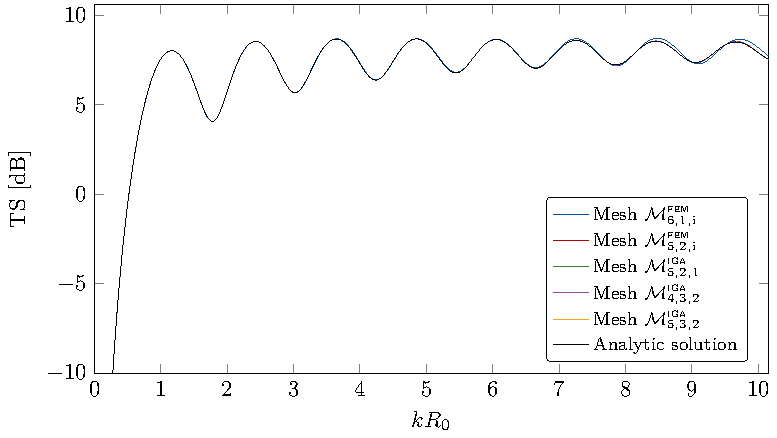
\includegraphics[width=\textwidth]{ihlenburg_farField_TSPlotSHBC}
	\caption{\textbf{Ihlenburg benchmark with SHBC}: The target strength (TS) in \Cref{Eq2:TS} is plotted against $kR_0$.}
	\label{Fig2:TSPlotSHBC}
	\par\bigskip
	\par\bigskip
	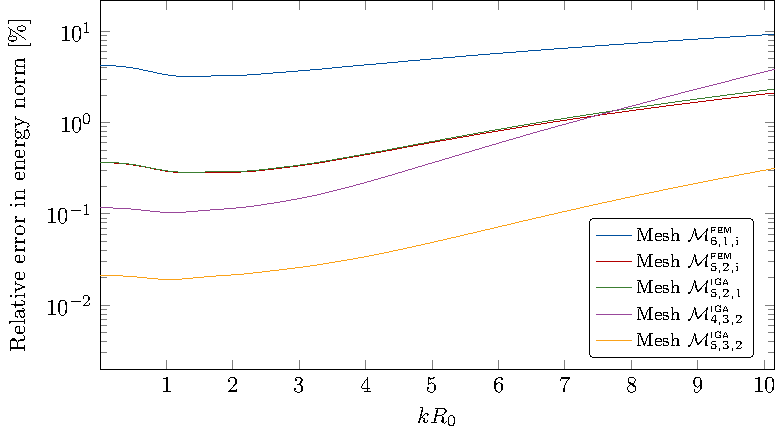
\includegraphics[width=\textwidth]{ihlenburg_farField_errorPlotSHBC}
	\caption{\textbf{Ihlenburg benchmark with SHBC}: The relative energy norm (\Cref{Eq2:energyNorm}) is plotted against $kR_0$.}
	\label{Fig2:errorPlotSHBC}
\end{figure}
\begin{figure}
	\centering
	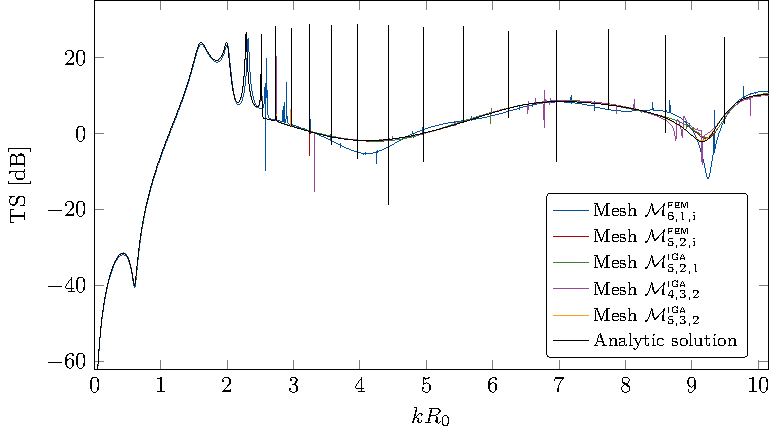
\includegraphics[width=\textwidth]{ihlenburg_farField_TSPlotSSBC}
	\caption{\textbf{Ihlenburg benchmark with SSBC}: ASI problem with the internal pressure modeled to be $p_2=0$. The target strength (TS) in \Cref{Eq2:TS} is plotted against $kR_0$.}
	\label{Fig2:TSPlotSSBC}
	\par\bigskip
	\par\bigskip
	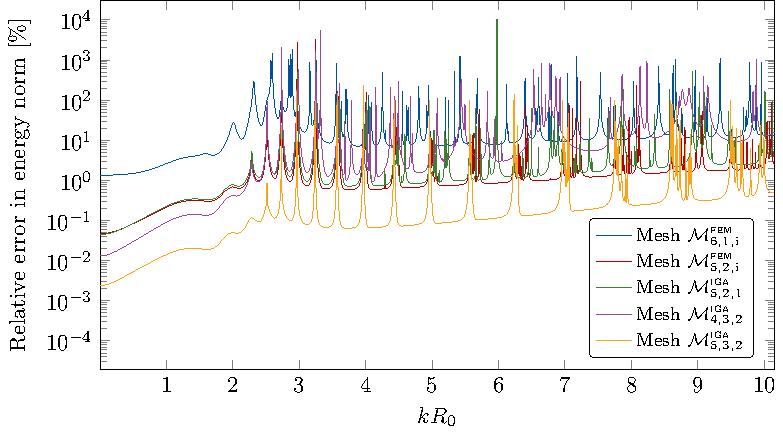
\includegraphics[width=\textwidth]{ihlenburg_farField_errorPlotSSBC}
	\caption{\textbf{Ihlenburg benchmark with SSBC}: ASI problem with the internal pressure modeled to be $p_2=0$. The relative energy norm (\Cref{Eq2:energyNorm}) is plotted against $kR_0$.}
	\label{Fig2:errorPlotSSBC}
\end{figure}
\begin{figure}
	\centering
	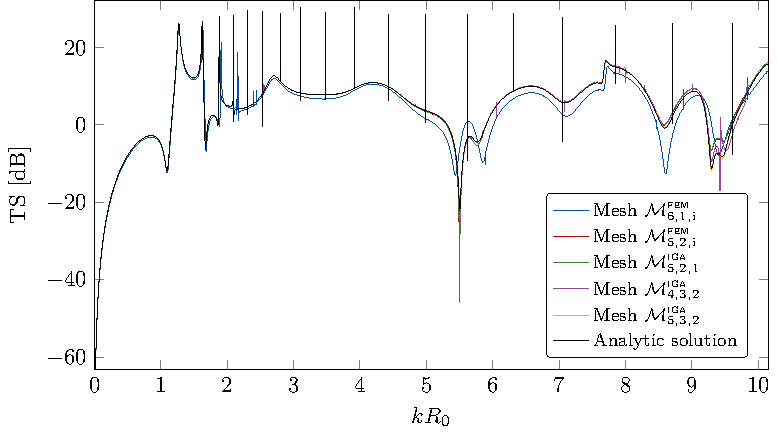
\includegraphics[width=\textwidth]{ihlenburg_farField_TSPlotNNBC}
	\caption{\textbf{Ihlenburg benchmark with NNBC}: The target strength (TS) in \Cref{Eq2:TS} is plotted against $kR_0$.}
	\label{Fig2:TSPlotNNBC}
	\par\bigskip
	\par\bigskip
	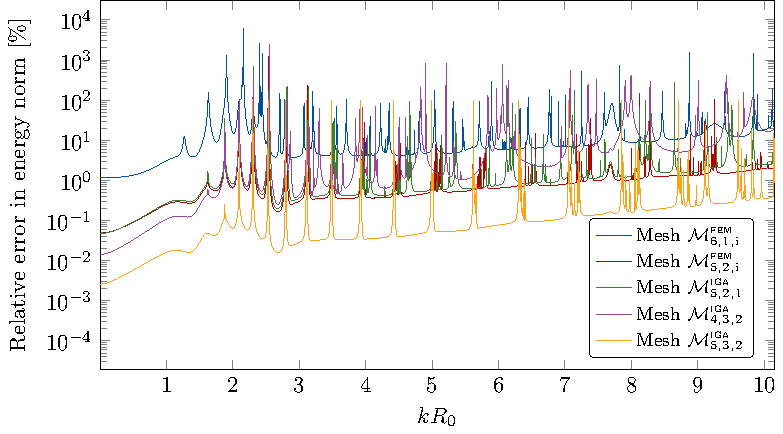
\includegraphics[width=\textwidth]{ihlenburg_farField_errorPlotNNBC}
	\caption{\textbf{Ihlenburg benchmark with NNBC}: The relative energy norm (\Cref{Eq2:energyNorm}) is plotted against $kR_0$.}
	\label{Fig2:errorPlotNNBC}
\end{figure}
In \Cref{Fig2:energyErrorPlot} we visualize the distribution of the error of the full ASI problem. The error is observed to be largest at element boundaries where the continuity is reduced. Since second order basis functions are used and the error in the velocity/stress dominates the error in the pressure/displacement, the results are in agreement with what was observed in \cite{Kumar2017spr}, i.e., that the error in the derivative of the primary solution is largest at the element boundaries.
\begin{figure}
	\centering
	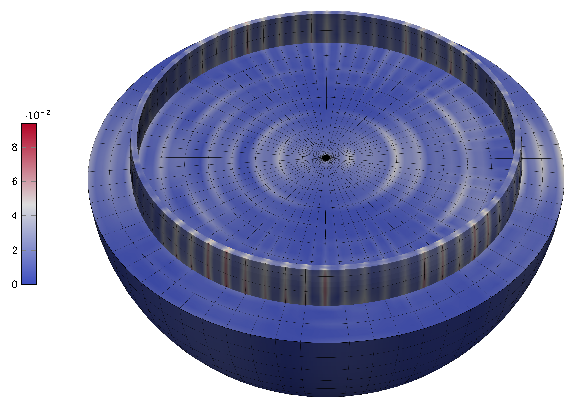
\includegraphics[width=0.7\textwidth]{energyErrorPlot}
	\caption{\textbf{Ihlenburg benchmark with NNBC}: Simulation of the full ASI problem on mesh ${\cal M}_{5,2,1}^{\textsc{iga}}$. Pointwise evaluation of the square root of the integrand of the volume integrals in the energy norm $\energyNorm{U-U_h}{\Omega}$ in \Cref{Eq2:energyNorm} with $k=\SI{2}{m^{-1}}$ (error in the infinite elements in $\Omega_{\mathrm{a}}^+$ is not shown) is here visualized, where $U$ is the set of analytic solutions in both fluid domains and the solid domain, and $U_h$ is the corresponding numerical solution. The values are scaled by the square root of the maximum of the corresponding integrand values of $\energyNorm{U}{\Omega}$. Both fluid domains are cut open at the $xy$-plane (at $z=0$), and the solid domain is cut open at $z=\SI{1.1}{m}$.}
	\label{Fig2:energyErrorPlot}
\end{figure}

\subsection{Radial pulsation from a mock shell}
\label{Subsec2:mockShell}
By construction of the fundamental solution of the Helmholtz equation ($\Phi_k(\vec{x},\vec{y})$ in \Cref{Eq2:FreeSpaceGrensFunction}), the function $p(\vec{x}) = \Phi_k(\vec{x},\vec{y})$ is a solution to \Cref{Eq2:HelmholtzEqn,Eq2:HelmholtzEqnNeumannCond,Eq2:sommerfeldCond} whenever $\vec{y}\in\R^3\setminus\overline{\Omega^+}$ and for the Neumann boundary condition $g(\vec{x})=\partial_n\Phi_k(\vec{x},\vec{y})$ on $\Gamma_0$.  Hence, we have an exact reference solution for the exterior Helmholtz problem for arbitrary geometries $\Gamma_0$ which encloses the point $\vec{y}$. It is emphasized that this solution is non-physical for non-spherical geometries $\Gamma_0$. General solutions may be constructed by separation of variables (cf.~\cite[p. 26]{Ihlenburg1998fea})
\begin{equation}
	p(\vec{x}) = \sum_{n=0}^\infty\sum_{m=-n}^n C_{nm} \hankel_n^{(1)}(kR) \legendre_n^{|m|}(\cos\vartheta)\euler^{\imag m\varphi} 
\end{equation}
with
\begin{equation*}
	R = |\vec{x}-\vec{y}|,\quad \vartheta=\arccos\left(\frac{x_3-y_3}{R}\right),\quad\varphi = \operatorname{atan2}(x_2-y_2,x_1-y_1)
\end{equation*}
where $\hankel_n^{(1)}$ is the $n^{\mathrm{th}}$ spherical Hankel function of first kind and $\legendre_n^m$ are the associated Legendre functions. In fact, the solution $p(\vec{x}) = \Phi_k(\vec{x},\vec{y})$ is a special case of this general form with 
\begin{equation}
	C_{nm} = \begin{cases}
		\frac{\imag k}{4\PI} & n = 0,\,\,m=0\\
		0 & \text{otherwise}.
		\end{cases}
\end{equation}
The complexity of this problem setup does not scale with the complexity of the model as it is independent of $\Gamma_0$. However, it preserves two important properties of acoustic scattering, namely the radial decay and the oscillatory nature. Thus, this problem setup represents a general way of constructing manufactured solutions, that can be utilized to verify the correctness of the implemented code for solving the Helmholtz equation. A special case of this general setup is the pulsating sphere example in~\cite{Simpson2014aib}.

From the first limit of \Cref{Eq2:Phi_k_limits1,Eq2:Phi_k_limits2}, the far field is given by $p_0(\hat{\vec{x}})=\frac{1}{4\PI}\euler^{-\imag k \hat{\vec{x}}\cdot\vec{y}}$. Thus, the target strength is a constant, $\TS=-20\log_{10}(4\PI)\approx -21.984$ (where we define $P_{\mathrm{inc}}=\SI{1}{Pa}$ in \Cref{Eq2:TS} for this problem). 

Consider the case $\vec{y}=\frac{R_0}{4}(1,1,1)$ and the boundary $\Gamma_0$ given by a \textit{mock shell} composed of a cylinder with hemispherical endcaps (with axis of symmetry along the $x$-axis such that the center of the spherical endcaps are located at $x = 0$ and $x = -L$). The cylinder has radius $R_0=\SI{1}{m}$ and length $L=\frac{\PI}{2}R_0$. The analytic solution is given by
\begin{equation}
	p(\vec{x}) = \frac{\euler^{\imag kR}}{4\PI R},\quad R=|\vec{x}-\vec{y}|
\end{equation}
and the Neumann condition is then
\begin{equation}
	g(\vec{x}) = \frac{\euler^{\imag kR}}{4\PI R^3}(\imag kR -1) (\vec{x}-\vec{y})\cdot\vec{n}(\vec{x}).
\end{equation}

This example is used to illustrate the differences of the infinite element formulations using the prolate ellipsoidal elements after Burnett~\cite{Burnett1994atd}. The mesh construction is illustrated in \Cref{Fig2:MS_meshes}, and an illustration of the solution is presented in \Cref{Fig2:MS_visualization}.
\begin{figure}
	\centering    
	\begin{subfigure}{0.49\textwidth}
		\centering
		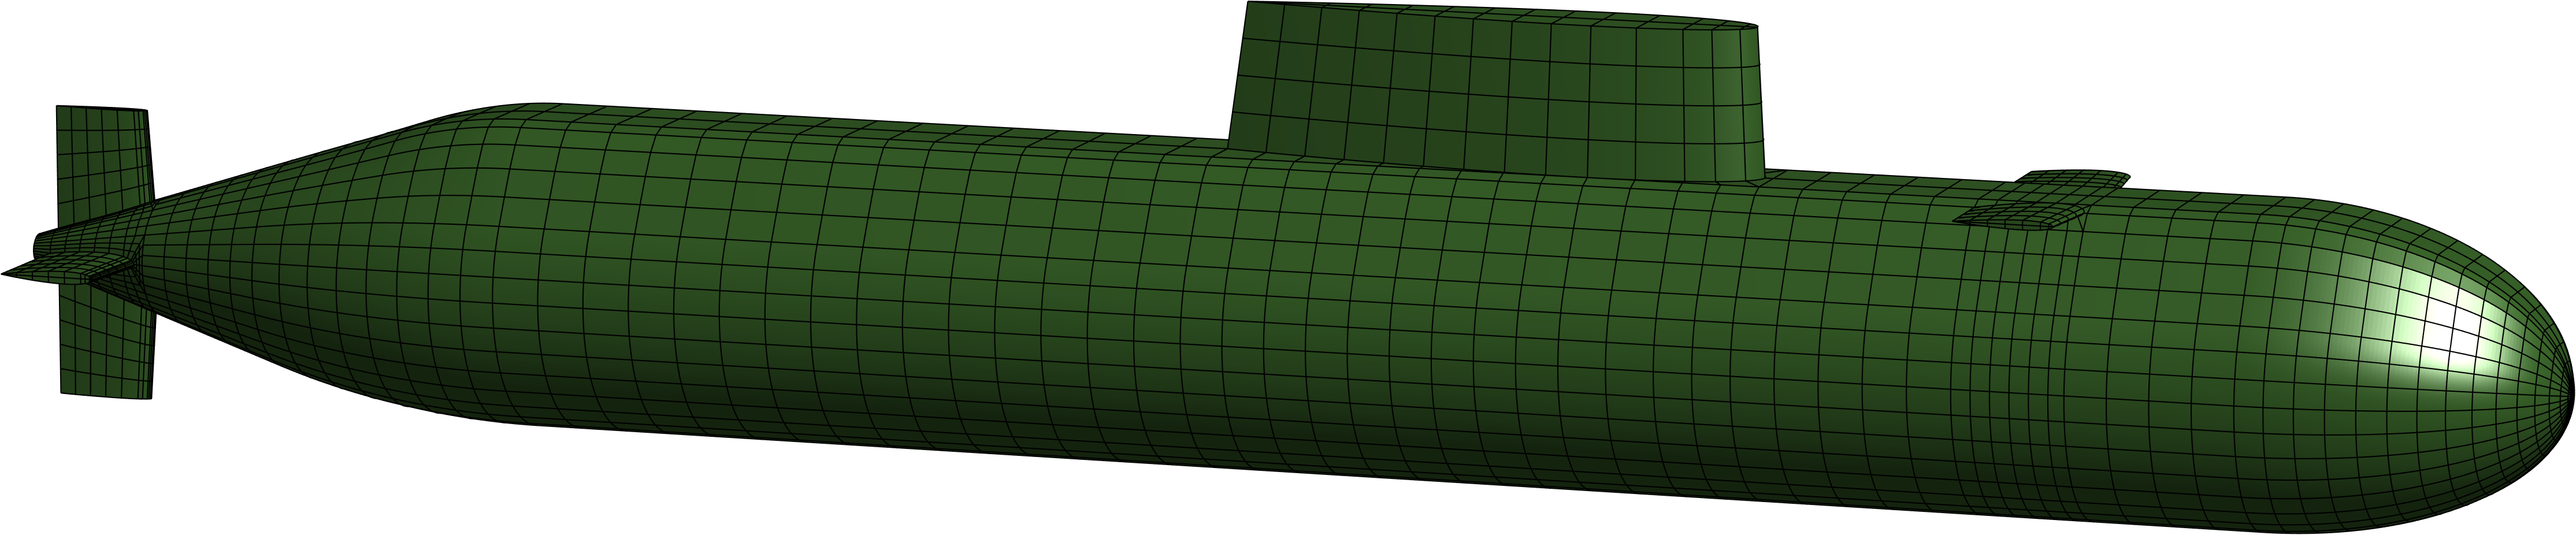
\includegraphics[width=\textwidth]{mesh1}
		\caption{Mesh 1.}
	\end{subfigure}%
	\hspace*{0.02\textwidth}%
	\begin{subfigure}{0.49\textwidth}
		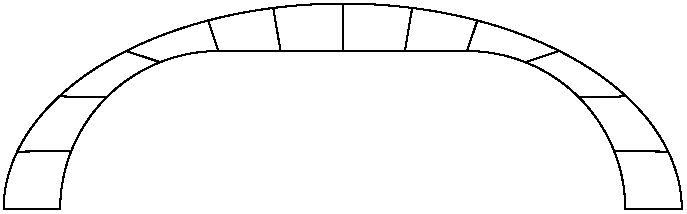
\includegraphics[width=\textwidth]{mesh3}
		\caption{Mesh 3.}
	\end{subfigure}
	\par\bigskip
	\begin{subfigure}{0.49\textwidth}
		\centering
		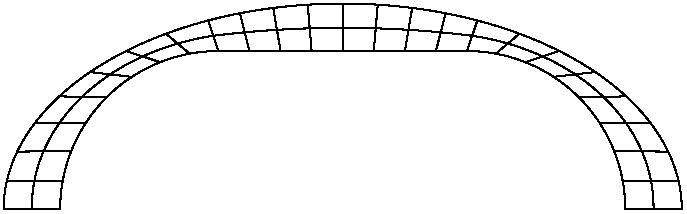
\includegraphics[width=\textwidth]{mesh4}
		\caption{Mesh 4.}
	\end{subfigure}%
	\hspace*{0.02\textwidth}%
	\begin{subfigure}{0.49\textwidth}
		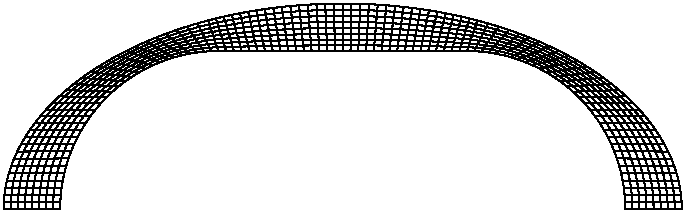
\includegraphics[width=\textwidth]{mesh6}
		\caption{Mesh 6.}
	\end{subfigure}
	\caption{\textbf{Radial pulsation from a mock shell}: Meshes for the fluid domain between the scatterer and the artificial boundary. The meshes are constructed from the initial mesh 1, which is rotated around the axis of symmetry using four elements. Mesh 2 and 3 are refined only in the angular direction, while the more refined meshes also refine in the radial direction to obtain smallest aspect ratio. The meshes are nested.}
	\label{Fig2:MS_meshes}
\end{figure}
\begin{figure}
	\centering
	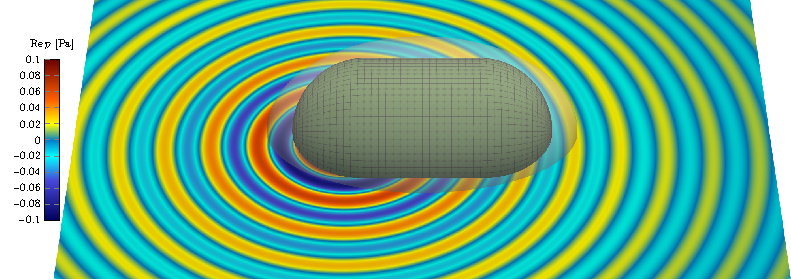
\includegraphics[width=\textwidth]{MS_PnearField}
	\caption{\textbf{Radial pulsation from a mock shell}: Visualization of numerical solution in the $xy$-plane using BGU with $N=6$ on mesh 5.}
	\label{Fig2:MS_visualization}
\end{figure}
Convergence plots are shown in \Cref{Fig2:MS_convergence}. Gerdes did a similar comparison in~\cite{Gerdes1998tcv} where scattering on a sphere was investigated. Our results verify these findings, namely lower errors for the unconjugated formulations (cf. \Cref{Fig2:MS_convergence}). Good results can be obtained using only a single radial shape function in case of unconjugated formulations. For the conjugated versions, on the other hand, $N > 6$ functions are needed to obtain similar accuracy and more degrees of freedom are required to get an asymptotic behavior.

In \Cref{Fig2:MS_condNumbersB} and \Cref{Fig2:MS_condNumbersP} the condition number is investigated for the different formulations and basis functions in the radial shape functions. The condition number for the unconjugated versions increases more rapidly as a function of $N$ compared to the corresponding formulations in the conjugated case. The condition number of the Lagrange basis increases particularly fast with $N$, making it useless\footnote{In the case of $r_n = nr_{\mathrm{a}}$.} for the conjugated formulations. However, the Lagrange basis yields the best result for the unconjugated formulations for small $N$. The Chebyshev basis seems to give the best condition numbers for the conjugated formulations for large $N$ (which is required for acceptable results). The unconjugated formulations perform quite similar, both in terms of the condition numbers and the error. The BGU formulation has the additional advantage of producing symmetric matrices and reduces the memory requirement. 
\begin{figure}
	\centering    
	\begin{subfigure}{0.49\textwidth}
		\centering
		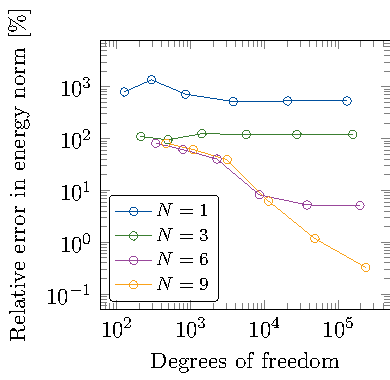
\includegraphics[width=\textwidth]{mockShellConvergence_1}
	\caption{BGC}
	\end{subfigure}%
	\hspace*{0.02\textwidth}%
	\begin{subfigure}{0.49\textwidth}
		\centering
		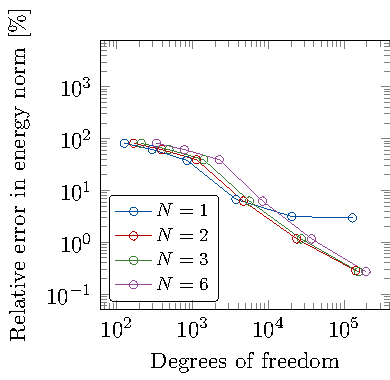
\includegraphics[width=\textwidth]{mockShellConvergence_2}
		\caption{BGU}
	\end{subfigure}%
	\par\bigskip
	\par\bigskip
	\begin{subfigure}{0.49\textwidth}
		\centering
		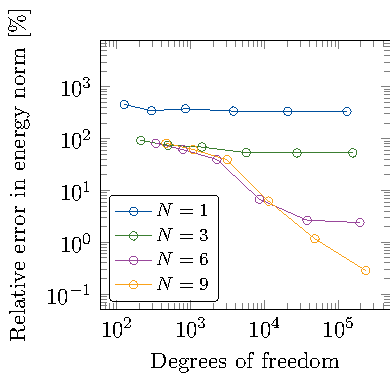
\includegraphics[width=\textwidth]{mockShellConvergence_3}
		\caption{PGC}
	\end{subfigure}%
	\hspace*{0.02\textwidth}%
	\begin{subfigure}{0.49\textwidth}
		\centering
		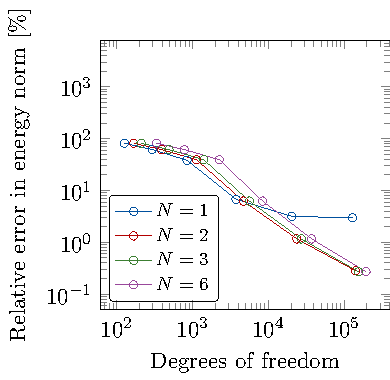
\includegraphics[width=\textwidth]{mockShellConvergence_4}
		\caption{PGU}
	\end{subfigure}%
	\caption{\textbf{Radial pulsation from a mock shell}: Convergence plots for the four infinite element formulations. The relative error in the energy norm (\Cref{Eq2:energyNormFluids}) is plotted against the number of degrees of freedom.}
	\label{Fig2:MS_convergence}
\end{figure}

\begin{figure}
	\begin{subfigure}{0.49\textwidth}
		\centering
		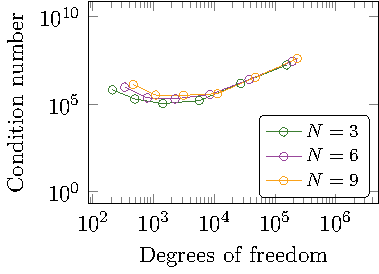
\includegraphics{mockShellConvergence_5}
		\caption{BGC with the shifted Chebyshev basis}
	\end{subfigure}%
	\hspace*{0.02\textwidth}%
	\begin{subfigure}{0.49\textwidth}
		\centering
		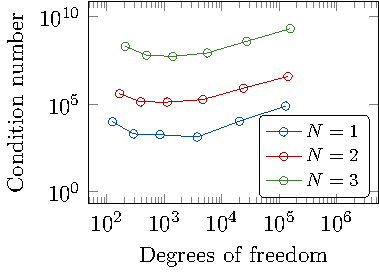
\includegraphics{mockShellConvergence_6}
		\caption{BGU with the shifted Chebyshev basis}
	\end{subfigure}
	\par\bigskip
	\begin{subfigure}{0.49\textwidth}
		\centering
		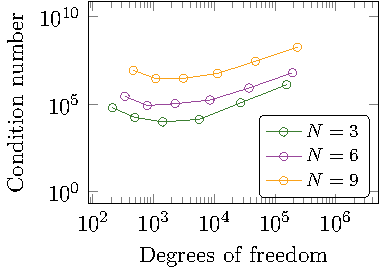
\includegraphics{mockShellConvergence_7}
		\caption{BGC with the Bernstein basis}
	\end{subfigure}%
	\hspace*{0.02\textwidth}%
	\begin{subfigure}{0.49\textwidth}
		\centering
		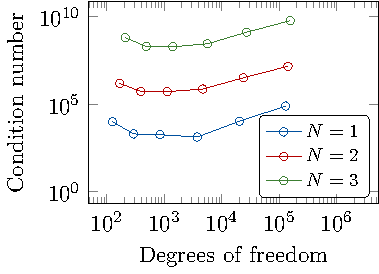
\includegraphics{mockShellConvergence_8}
		\caption{BGU with the Bernstein basis}
	\end{subfigure}
	\par\bigskip
	\begin{subfigure}{0.49\textwidth}
		\centering
		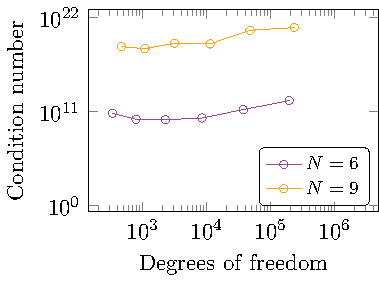
\includegraphics{mockShellConvergence_9}
		\caption{BGC with the Lagrange basis}
	\end{subfigure}%
	\hspace*{0.02\textwidth}%
	\begin{subfigure}{0.49\textwidth}
		\centering
		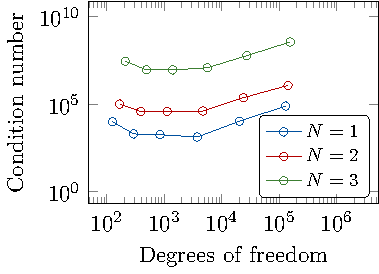
\includegraphics{mockShellConvergence_10}
		\caption{BGU with the Lagrange basis}
	\end{subfigure}
	\caption{\textbf{Radial pulsation from a mock shell}: Convergence plots for the BGC and BGU formulations using three different sets of radial shape functions (Chebyshev, Bernstein and Lagrange). The condition number (1-norm condition number estimate provided by \texttt{condest} in \MATLAB) is plotted against the number of degrees of freedom.}
	\label{Fig2:MS_condNumbersB}
\end{figure}


\begin{figure}
	\begin{subfigure}{0.49\textwidth}
		\centering
		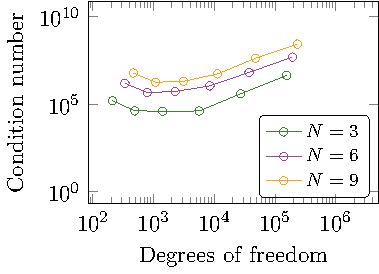
\includegraphics{mockShellConvergence_11}
		\caption{PGC with the shifted Chebyshev basis}
	\end{subfigure}%
	\hspace*{0.02\textwidth}%
	\begin{subfigure}{0.49\textwidth}
		\centering
		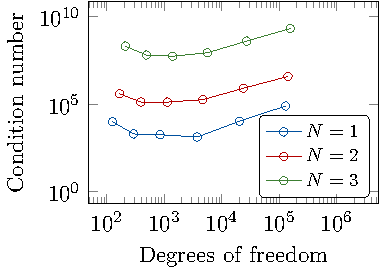
\includegraphics{mockShellConvergence_12}
		\caption{PGU with the shifted Chebyshev basis}
	\end{subfigure}
	\par\bigskip
	\begin{subfigure}{0.49\textwidth}
		\centering
		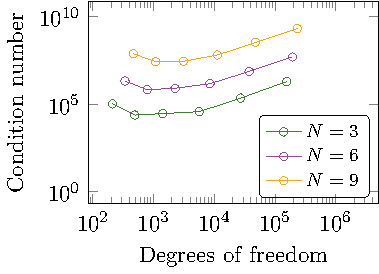
\includegraphics{mockShellConvergence_13}
		\caption{PGC with the Bernstein basis}
	\end{subfigure}%
	\hspace*{0.02\textwidth}%
	\begin{subfigure}{0.49\textwidth}
		\centering
		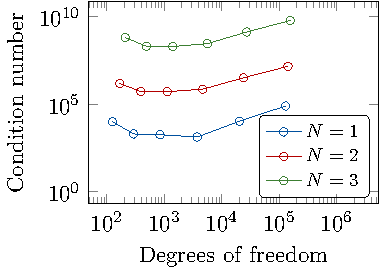
\includegraphics{mockShellConvergence_14}
		\caption{PGU with the Bernstein basis}
	\end{subfigure}
	\par\bigskip
	\begin{subfigure}{0.49\textwidth}
		\centering
		\includegraphics{mockShellConvergence_15}
		\caption{PGC with the Lagrange basis}
	\end{subfigure}%
	\hspace*{0.02\textwidth}%
	\begin{subfigure}{0.49\textwidth}
		\centering
		\includegraphics{mockShellConvergence_16}
		\caption{PGU with the Lagrange basis}
	\end{subfigure}
	\caption{\textbf{Radial pulsation from a mock shell}: Convergence plots for the PGC and PGU formulations using three different sets of radial shape functions (Chebyshev, Bernstein and Lagrange). The condition number (1-norm condition number estimate provided by \texttt{condest} in \MATLAB) is plotted against the number of degrees of freedom.}
	\label{Fig2:MS_condNumbersP}
\end{figure}

It is clear that the choice of basis functions in the infinite elements plays a crucial role for the condition number, and more research is required to find the optimal set of basis functions. Based on the findings in this work, it is recommended to use the BGU formulation alongside the Lagrange basis (in the radial direction) in the infinite elements. However, if larger $N$ is needed for accuracy, the Chebyshev basis is recommended.

\subsection{Stripped BeTSSi submarine}
Finally, we consider the \textit{stripped BeTSSi submarine}\footnote{Based upon the BeTSSi submarine which originates from the BeTSSi workshops~\cite{Gilroy2013bib}.} described in \Cref{Sec2:BeTSSi_description}. 

Let a plane wave, with the direction of incidence given by
\begin{equation}
	\vec{d}_{\mathrm{s}} = -\begin{bmatrix}
		\cos\beta_{\mathrm{s}}\cos\alpha_{\mathrm{s}}\\
		\cos\beta_{\mathrm{s}}\sin\alpha_{\mathrm{s}}\\
		\sin\beta_{\mathrm{s}}
	\end{bmatrix}, \quad\text{where}\quad \alpha_{\mathrm{s}} = \ang{240},\,\beta_{\mathrm{s}} = \ang{0},
\end{equation}
be scattered by this submarine. The CAD model is given in \Cref{Fig2:BC_strippedAndMesh} alongside computational meshes. Again, we shall denote by ${\cal M}_{m,\check{p},\check{k}}^{\textsc{iga}}$, mesh number $m$ with polynomial order $\check{p}$ and continuity $\check{k}$ across element boundaries of the NURBS parametrization. 

\begin{figure}
	\begin{subfigure}{\textwidth}
		\centering
		\includegraphics[width=0.95\textwidth]{BeTSSi_BC_stripped}
		\caption{CAD model.}
		\label{Fig2:BC_stripped}
	\end{subfigure}
	\par\bigskip
	\par\bigskip
	\begin{subfigure}{\textwidth}
		\centering
		\includegraphics[width=0.95\textwidth]{BeTSSi_BC_mesh1}
		\caption{Surface mesh for mesh ${\cal M}_{1,\check{p},\check{k}}^{\mathrm{IGA}}$}
	\end{subfigure}	
	\par\bigskip
	\par\bigskip
	\begin{subfigure}{\textwidth}
		\centering
		\includegraphics[width=0.95\textwidth]{BeTSSi_BC_mesh2}
		\caption{Surface mesh for mesh ${\cal M}_{2,\check{p},\check{k}}^{\mathrm{IGA}}$.}
	\end{subfigure}	
	\par\bigskip
	\par\bigskip
	\begin{subfigure}{\textwidth}
		\centering
		\includegraphics[width=0.95\textwidth]{BeTSSi_BC_mesh1_eta}
		\caption{Crossection in the $xz$-plane for mesh ${\cal M}_{1,\check{p},\check{k}}^{\mathrm{IGA}}$.}
	\end{subfigure}	
	\par\bigskip
	\par\bigskip
	\begin{subfigure}{\textwidth}
		\centering
		\includegraphics[width=0.95\textwidth]{BeTSSi_BC_mesh2_eta}
		\caption{Crossection in the $xz$-plane for mesh ${\cal M}_{2,\check{p},\check{k}}^{\mathrm{IGA}}$.}
	\end{subfigure}	
	\caption{\textbf{Stripped BeTSSi submarine}: CAD model and meshes used for computations.}
	\label{Fig2:BC_strippedAndMesh}
\end{figure}
The near field at $f=\SI{1000}{Hz}$ is visualized in \Cref{Fig2:BC_NearField}.
\begin{figure}
	\centering    
	\begin{subfigure}[b]{\textwidth}
		\centering
		\includegraphics[width=\textwidth]{BC_nearField_1}
		\caption{Real part of the incident wave $p_{\mathrm{inc}}(\vec{x})=P_{\mathrm{inc}}\euler^{\imag k\vec{d}_{\mathrm{s}}\cdot \vec{x}}$.}
	\end{subfigure}
	\par\bigskip
	\begin{subfigure}[b]{\textwidth}
		\centering
		\includegraphics[width=\textwidth]{BC_nearField_2}
		\caption{Real part of the scattered pressure $p(\vec{x})$.}
	\end{subfigure}
	\par\bigskip
	\begin{subfigure}[b]{\textwidth}
		\centering
		\includegraphics[width=\textwidth]{BC_nearField_3}
		\caption{Real part of the total pressure $p_{\mathrm{tot}}(\vec{x})=p_{\mathrm{inc}}(\vec{x})+p(\vec{x})$.}
	\end{subfigure}
	\par\bigskip
	\begin{subfigure}[b]{\textwidth}
		\centering
		\includegraphics[width=\textwidth]{BC_nearField_4}
		\caption{Modulus of the total pressure $p_{\mathrm{tot}}(\vec{x})=p_{\mathrm{inc}}(\vec{x})+p(\vec{x})$.}
	\end{subfigure}
	\caption{\textbf{Stripped BeTSSi submarine with SHBC}: The simulation at $f=\SI{1000}{Hz}$ is visualized in the $xy$-plane, and is computed on mesh ${\cal M}_{2,3,2}^{\mathrm{IGA}}$ and the BGU formulation with $N=4$. The numerical evaluations outside the (transparent) prolate ellipsoidal artificial boundary are evaluated with \Cref{Eq2:KirchhoffIntegral}.}
	\label{Fig2:BC_NearField}
\end{figure}
The low frequency problem at $f = \SI{100}{Hz}$ is considered in~\Cref{Fig2:FarField100}. In this case, mesh ${\cal M}_{1,2,1}^{\mathrm{IGA}}$ resolves this frequency, but the solution slightly deviates from the reference solution computed by IGABEM on a fine mesh. The reason for this is that $N$ is too low. Although $N=3$ was enough for engineering precision (below 1\%) in the mock shell example, it does not suffice for the more complicated geometry like the stripped BeTSSi submarine. Consider the relative error for the far field at the well resolved mesh ${\cal M}_{2,3,2}^{\mathrm{IGA}}$. In this case the error will originate from the low resolution (governed by $N$) in the radial direction for the infinite elements. As illustrated in \Cref{Fig2:FarField100error} an order of magnitude in accuracy is gained by increasing $N$. This effect was also observed by the verification test in \Cref{Subsec2:mockShell} applied to the stripped BeTSSi submarine.
\begin{figure}
	\centering    
	\includegraphics[width=\textwidth]{BC_farField100_1}
	\caption{\textbf{Stripped BeTSSi submarine with SHBC}: Computation of target strength (\Cref{Eq2:TS}) at $f=\SI{100}{Hz}$ as a function of the azimuth angle in the spherical coordinate system. The two IGA results (both using $N=3$) are visually indistinguishable meaning that mesh ${\cal M}_{1,2,1}^{\mathrm{IGA}}$ is well resolved for this frequency.}
	\label{Fig2:FarField100}
\end{figure}
\begin{figure}
	\centering    
	\includegraphics[width=\textwidth]{BC_farField100_2}
	\caption{\textbf{Stripped BeTSSi submarine with SHBC}: Computation of the relative error in the far field (\Cref{Eq2:KirchhoffIntegral}) compared to a reference solution at $f=\SI{100}{Hz}$. The computations are done using IGA on mesh ${\cal M}_{2,3,2}^{\mathrm{IGA}}$ using the BGU formulation.}
	\label{Fig2:FarField100error}
\end{figure}
In \Cref{Fig2:FarField} the target strength is plotted for $f=\SI{500}{Hz}$ and $f=\SI{1000}{Hz}$. A reference solution (using IGABEM) is added for the $f=\SI{500}{Hz}$ case, and illustrates again the pollution of low $N$. The IGA mesh 1 resolves the frequency $f=\SI{500}{Hz}$ quite well using only about 5 elements per wavelength. This corresponds to about 5 dofs per wavelength in each dimensional direction compared to the classical 10-12 dofs per wavelength needed for FEM methods.
\begin{figure}
	\centering    
	\begin{subfigure}[b]{\textwidth}
		\centering
		\includegraphics[width=\textwidth]{BC_farField_1}
		\caption{$f=\SI{500}{Hz}$}
	\end{subfigure}
	\par\bigskip
	\par\bigskip
	\begin{subfigure}[b]{\textwidth}
		\centering
		\includegraphics[width=\textwidth]{BC_farField_2}
		\caption{$f=\SI{1000}{Hz}$}
	\end{subfigure}
	\caption{\textbf{Stripped BeTSSi submarine with SHBC}: Computation of target strength (\Cref{Eq2:TS}) as a function of the azimuth angle in the spherical coordinate system. The numerical evaluations are evaluated with \Cref{Eq2:TS}.}
	\label{Fig2:FarField}
\end{figure}

%%\clearpage
\section{Conclusion}
\label{Sec4:conclusions}
This article addresses acoustic scattering characterized by sound waves reflected by man-made elastic objects. The present approach is characterized by:
\begin{itemize}
	\item The scattered pressure is approximated by Kirchhoff approximation.
	\item The computations are evaluated on the exact computer aided design model.
	\item The Helmholtz integrals are evaluated by the numerical steepest descent.
\end{itemize}

The main finding of the present study is that Kirchhoff approximation may be computed with a complexity independent of the frequency in the isogeometric analysis framework.

Furthermore, the following observations are made
\begin{itemize}
	\item The accuracy of the method converges as a function of the frequency, as opposed to a triangular approximation method where the accuracy diverges.
	\item The computational complexity of the Kirchhoff approximation method is at least one order less than finite/boundary element methods resulting in computational savings in orders of magnitudes. The cost of these savings is reduced accuracy, and for some geometries the Kirchhoff approximation simply is not applicable.
	\item The NSD formulation outperforms the triangulation approximation approach when considering the computational time as a function of the error or frequency.
\end{itemize}

The Kirchhoff approximation method in an isogeometric framework has good potential, but many challenges remains to be resolved before the presented code is fully automated.

Some challenges remain to be resolved for this work to be applicable to general CAD geometries. First, for each incident wave and for each element in the CAD mesh, all resonance and stationary points must be found. This could be implemented as a preprocessing step. Second, if the shadow boundary does not coincide with element boundaries, this must be resolved in the NSD algorithm. The parent domain will in this case not be rectangular, but rather parametrized boundary which requires special treatment in the NSD algorithm. Moreover, this challenge will affect the first challenge as potential resonance points may lie on the shadow boundary. Third, interior stationary points have not been considered in this work but is discussed in~\cite{Huybrechs2007tco}. Finally, rules must be established for the number of Gauss-Legendre points and Gauss-Laguerre points needed in the hybrid method.

To have an automated algorithm that tackles all of these challenges is a huge task. The integrals from the usage of curvilinear facets in~\cite{Lavia2018mhf} contains well behaved oscillatory functions ($g$ is second order polynomial) and may for this reason be a simpler approach. Especially since it is easier to discretize the scatterer, $\Gamma$, with curvilinear triangles in such a way that the shadow boundary lies on element edges.

\section*{Acknowledgements}
This work was supported by the Department of Mathematical Sciences at the Norwegian University of Science and Technology and by the Norwegian Defence Research Establishment.

We would like to thank Arieh Iserles for hosting us at our research stay at the Department of Applied Mathematics and Theoretical Physics at University of Cambridge (UK) during the fall of 2016. His guidance related to highly oscillatory integration is highly appreciated. We would also like to thank Daan Huybrechs at K.U. Leuven University (Belgium) for valuable comments about the numerical steepest descent method. 

%%\clearpage
%%
\begin{inputAppendices}
	\section{Coordinate systems}


\subsection{General 3D coordinate system}
\label{Sec2:general3DcoordinateSystem}
We shall now consider the general 3D coordinate system, which one may reduce to the the cylindrical coordinate system and the spherical coordinate system. Let the coordinate system be defined by
\begin{equation*}
	\vec{r} = \begin{bmatrix}
	x(\xi, \eta, \zeta)\\
	y(\xi, \eta, \zeta)\\
	z(\xi, \eta, \zeta)
\end{bmatrix} :	 \R^3\to\R^3, \quad  \begin{bmatrix}
	\xi\\
	\eta\\
	\zeta
	\end{bmatrix}\mapsto \vec{r}(\xi, \eta, \zeta).
\end{equation*}
We shall frequently use the scaling lengths defined by
\begin{align}
	h_{\upxi} &= \norm{\pderiv{\vec{r}}{\xi}} = \sqrt{\left(\pderiv{x}{\xi}\right)^2+\left(\pderiv{y}{\xi}\right)^2+\left(\pderiv{z}{\xi}\right)^2}\nonumber\\
	h_{\upeta} &= \norm{\pderiv{\vec{r}}{\eta}} = \sqrt{\left(\pderiv{x}{\eta}\right)^2+\left(\pderiv{y}{\eta}\right)^2+\left(\pderiv{z}{\eta}\right)^2}\label{Eq2:ScalingLengths}\\
	h_{\upzeta} &= \norm{\pderiv{\vec{r}}{\zeta}} = \sqrt{\left(\pderiv{x}{\zeta}\right)^2+\left(\pderiv{y}{\zeta}\right)^2+\left(\pderiv{z}{\zeta}\right)^2}.\nonumber
\end{align}
The standard basis vectors in this general coordinate system are then
\begin{equation*}
	\vec{e}_{\upxi} = \frac{1}{h_{\upxi}}\pderiv{\vec{r}}{\xi},\quad\vec{e}_{\upeta} = \frac{1}{h_{\upeta}}\pderiv{\vec{r}}{\eta},\quad\vec{e}_{\upzeta} = \frac{1}{h_{\upzeta}}\pderiv{\vec{r}}{\zeta}.
\end{equation*}
We now want to develop an expression for the nabla operator in terms of these unit vectors. In our coordinate system, the nabla operator is defined by
\begin{equation*}
	\nabla f = \vec{e}_{\upxi} g_{\upxi} +\vec{e}_{\upeta} g_{\upeta} +\vec{e}_{\upzeta} g_{\upzeta}.
\end{equation*}
where $g_{\upxi}$, $g_{\upeta}$ and $g_{\upzeta}$ are functionals of $f$ which are to be determined.

Moreover, the nabla operator satisfy
\begin{equation*}
	\diff f = \nabla f\cdot\diff \vec{r},
\end{equation*}
where (by the chain rule)
\begin{align*}
	\diff \vec{r} &= \pderiv{\vec{r}}{\xi}\diff\xi + \pderiv{\vec{r}}{\eta}\diff\eta + \pderiv{\vec{r}}{\zeta}\diff\zeta\\
	  &= h_{\upxi}\vec{e}_{\upxi} \diff\xi + h_{\upeta}\vec{e}_{\upeta} \diff\eta + h_{\upzeta}\vec{e}_{\upzeta} \diff\zeta.
\end{align*}
Using the chain rule once again, we also have
\begin{equation*}
	\diff f = \pderiv{f}{\xi} \diff\xi + \pderiv{f}{\eta} \diff\eta + \pderiv{f}{\zeta} \diff\zeta.
\end{equation*}
Combining the equations for $\diff f$ we get the relation
\begin{align}
	\pderiv{f}{\xi} \diff\xi + \pderiv{f}{\eta} \diff\eta + \pderiv{f}{\zeta} \diff\zeta &= \left(\vec{e}_{\upxi} g_{\upxi} +\vec{e}_{\upeta} g_{\upeta} +\vec{e}_{\upzeta} g_{\upzeta}\right)\cdot\left(h_{\upxi}\vec{e}_{\upxi} \diff\xi + h_{\upeta}\vec{e}_{\upeta} \diff\eta + h_{\upzeta}\vec{e}_{\upzeta} \diff\zeta\right)\\
	&=h_{\upxi}(g_{\upxi} +  \vec{e}_{\upxi}\cdot \vec{e}_{\upeta} g_{\upeta} +  \vec{e}_{\upxi}\cdot\vec{e}_{\upzeta} g_{\upzeta})\diff\xi\\
	&+h_{\upeta}(\vec{e}_{\upxi}\cdot \vec{e}_{\upeta} g_{\upxi} +  g_{\upeta} +  \vec{e}_{\upeta}\cdot\vec{e}_{\upzeta} g_{\upzeta})\diff\eta\\
	&+h_{\upzeta}(\vec{e}_{\upxi}\cdot \vec{e}_{\upzeta} g_{\upxi} +  \vec{e}_{\upeta}\cdot\vec{e}_{\upzeta} g_{\upeta}+  g_{\upzeta})\diff\zeta
\end{align}
where we have used the fact that $\vec{e}_{\upxi}\cdot\vec{e}_{\upxi}= 1$, $\vec{e}_{\upeta}\cdot\vec{e}_{\upeta}= 1$ and $\vec{e}_{\upzeta}\cdot\vec{e}_{\upzeta}= 1$. As the coefficients in front of $\diff\xi$, $\diff\eta$ and $\diff\zeta$ must be the same on both side, we get a system of equations given by
\begin{equation}\label{Eq2:systemNablaOperator}
\begin{alignedat}{4}
	 g_{\upxi} & {}+{} &  \vec{e}_{\upxi}\cdot \vec{e}_{\upeta} g_{\upeta} & {}+{} &  \vec{e}_{\upxi}\cdot\vec{e}_{\upzeta} g_{\upzeta} &= \frac{1}{h_{\upxi}}\pderiv{f}{\xi}\\
	\vec{e}_{\upxi}\cdot \vec{e}_{\upeta} g_{\upxi} & {}+{} &  g_{\upeta} & {}+{} & \vec{e}_{\upeta}\cdot\vec{e}_{\upzeta} g_{\upzeta} &= \frac{1}{h_{\upeta}}\pderiv{f}{\eta}\\
	\vec{e}_{\upxi}\cdot \vec{e}_{\upzeta} g_{\upxi} & {}+{} & \vec{e}_{\upeta}\cdot\vec{e}_{\upzeta} g_{\upeta} & {}+{} & g_{\upzeta} &= \frac{1}{h_{\upzeta}}\pderiv{f}{\zeta}.
\end{alignedat}
\end{equation}
Introducing the notation
\begin{equation*}
	E_{\upxi\upeta} = \vec{e}_{\upxi}\cdot\vec{e}_{\upeta},\quad E_{\upxi\upzeta} = \vec{e}_{\upxi}\cdot\vec{e}_{\upzeta},\quad E_{\upeta\upzeta} = \vec{e}_{\upeta}\cdot\vec{e}_{\upzeta}
\end{equation*}
the system in \Cref{Eq2:systemNablaOperator} is given by can be written as
\begin{equation*}
	\begin{bmatrix}
		1 & E_{\upxi\upeta} & E_{\upxi\upzeta}\\
		E_{\upxi\upeta} & 1 & E_{\upeta\upzeta}\\
		E_{\upxi\upzeta} & E_{\upeta\upzeta} & 1\\
	\end{bmatrix}\begin{bmatrix}
		g_{\upxi}\\
		g_{\upeta}\\
		g_{\upzeta}
	\end{bmatrix} = \begin{bmatrix}
	\frac{1}{h_{\upxi}} \pderiv{f}{\xi}\\
	\frac{1}{h_{\upeta}} \pderiv{f}{\eta}\\
	\frac{1}{h_{\upzeta}} \pderiv{f}{\zeta}\end{bmatrix}.
\end{equation*}
As the determinant of this system of equation is given by
\begin{equation*}
	\nabla^2 = 1 - E_{\upxi\upeta}^2 - E_{\upxi\upzeta}^2 - E_{\upeta\upzeta}^2 + 2E_{\upxi\upeta}E_{\upxi\upzeta}E_{\upeta\upzeta}
\end{equation*}
we may write the solution as
\begin{align*}
\begin{bmatrix}
	g_{\upxi}\\
	g_{\upeta}\\
	g_{\upzeta}
\end{bmatrix} = \begin{bmatrix}
	a_{11} & a_{12} & a_{13}\\
	a_{21} & a_{22} & a_{23}\\
	a_{31} & a_{32} & a_{33}
\end{bmatrix} \begin{bmatrix}
	\frac{1}{h_{\upxi}} \pderiv{f}{\xi}\\
	\frac{1}{h_{\upeta}} \pderiv{f}{\eta}\\
	\frac{1}{h_{\upzeta}} \pderiv{f}{\zeta}
\end{bmatrix}
\end{align*}
where the coefficients $a_{ij}$ are given by the symmetric matrix
\begin{equation*}
	[a_{ij}] = \frac{1}{\nabla^2}\begin{bmatrix}
		1-E_{\upeta\upzeta}^2 & E_{\upxi\upzeta}E_{\upeta\upzeta} - E_{\upxi\upeta}  &  E_{\upxi\upeta}E_{\upeta\upzeta} - E_{\upxi\upzeta}\\
		E_{\upxi\upzeta}E_{\upeta\upzeta} - E_{\upxi\upeta} & 1-E_{\upxi\upzeta}^2 & E_{\upxi\upeta}E_{\upxi\upzeta} - E_{\upeta\upzeta}\\
		E_{\upxi\upeta}E_{\upeta\upzeta} - E_{\upxi\upzeta} & E_{\upxi\upeta}E_{\upxi\upzeta} - E_{\upeta\upzeta} & 1-E_{\upxi\upeta}^2
	\end{bmatrix}
\end{equation*}
Let's verify this calculation by finding the nabla operator in the spherical coordinate system. Letting $\xi$ correspond to the azimuthal angle $\phi$, $\eta$ the polar angle $\vartheta$ and $\zeta$ the radial direction $r$, we have the relations
\begin{align*}
	x &= \zeta\sin\eta\cos\xi\\
	y &= \zeta\sin\eta\sin\xi\\
	z &= \zeta\cos\eta.
\end{align*}
As the spherical coordinate system is an orthogonal coordinate system, we get $E_{\upxi\upeta}=0$, $E_{\upxi\upzeta}=0$ and $E_{\upeta\upzeta}=0$. Thus,
\begin{equation*}
	g_{\upxi} = \frac{1}{h_{\upxi}}\pderiv{f}{\xi},\quad g_{\upeta} =\frac{1}{h_{\upeta}}\pderiv{f}{\eta},\quad g_{\upzeta} =\frac{1}{h_{\upzeta}}\pderiv{f}{\zeta}.
\end{equation*}
By computation, we find
\begin{equation*}
	h_{\upxi} = \zeta\sin\eta,\quad h_{\upeta} = \zeta,\quad h_{\upzeta} = 1.
\end{equation*}
Thus,
\begin{align*}
	\nabla f &= \frac{1}{\zeta\sin\eta}\pderiv{f}{\xi}\vec{e}_{\upxi} + \frac{1}{\zeta}\pderiv{f}{\eta}\vec{e}_{\upeta} + \pderiv{f}{\zeta}\vec{e}_{\upzeta}\\
	&= \pderiv{f}{r}\vec{e}_{\mathrm{r}} + \frac{1}{r}\pderiv{f}{\vartheta}\vec{e}_{\upvartheta} + \frac{1}{r\sin\vartheta}\pderiv{f}{\phi}\vec{e}_{\upphi},
\end{align*}
which is the familiar expression for the nabla operator in spherical coordinates.

\subsubsection{Extended NURBS coordinate system}
\label{subsubsubsec:infElementsOnGeneralizedCoordSyst}
In this section we shall explore the possibility to have a more general coordinate system for the infinite elements. All though the prolate spheroidal coordinate system helps reduce the number of elements needed to circumference a long obstacle compared to the spherical coordinate system, it is still not ideal with respect to this problem. It is possible to define a coordinate system such that we get
\begin{equation*}
	\inf_{\vec{x}\in\Gamma} \| \vec{x} - \vec{y}_0 \| = \inf_{\vec{y}\in\Gamma_{\mathrm{a}}} \| \vec{x}_0-\vec{y}\|\quad \forall\vec{x}_0\in\Gamma,\quad\text{and}\quad\forall\vec{y}_0\in\Gamma_{\mathrm{a}}.
\end{equation*}
That is, we can have the surface $\Gamma_{\mathrm{a}}$ at a constant distance from the surface $\Gamma$ (if $\Gamma$ is convex\footnote{If this is not the case, an intermediate convex surface must be inserted between $\Gamma$ and $\Gamma_{\mathrm{a}}$ in the NURBS patch.}). However, is it possible to define a infinite element formulation on such a coordinate system? The most intuitive coordinate system would satisfy the property that for all points on $\Gamma_{\mathrm{a}}$ the normal vector is parallel to the ``radial'' unit vector for this coordinate system. This would however make the integration in the weak formulation hard as the nabla operator would not be separable, and we may no longer integrate analytically in the ``radial'' direction. In the following we shall consider another option which results in a separable nabla operator.

Let's build upon the theory developed in \Cref{Sec2:general3DcoordinateSystem} where we shall assume that the NURBS parametrization at hand has a ``radial'' parameter $\zeta$, such that $\xi$ and $\eta$ corresponds to ``angular'' parameters. This will typically be the case when considering shell objects, where $\zeta$ will run through the thickness of the elastic material. We know that at any given value $\bar{\zeta}$ the NURBS solid in 3D reduces to a NURBS surface in 3D. This is in particular true for $\bar{\zeta} = 1$, which will be our artificial boundary $\Gamma_{\mathrm{a}}$. We shall assume, without loss of generality, that the NURBS surface $\Gamma_{\mathrm{a}}$ fully encloses the origin. Finally, we assume the surface $\Gamma_{\mathrm{a}}$ to be a convex surface. We now want to extend the NURBS parametrization also for $\zeta > 1$. In particular we define (for $\zeta>1$)
\begin{equation*}
	\vec{r} = \begin{bmatrix}
	x(\xi, \eta, \zeta)\\
	y(\xi, \eta, \zeta)\\
	z(\xi, \eta, \zeta)
\end{bmatrix} :	 \R^3\to\R^3, \quad  \begin{bmatrix}
	\xi\\
	\eta\\
	\zeta
	\end{bmatrix}\mapsto s(\zeta)\bar{\vec{r}}(\xi, \eta).
\end{equation*}
where $\bar{\vec{r}}$ is the NURBS 3D surface at $\zeta = 1$ and the \textit{scaling function} $s$ is strictly increasing and satisfies $s(1) = 1$. Thus, for any $\zeta > 1$ we simply get a scaled version of $\Gamma_{\mathrm{a}}$ from the origin with the scaling factor $s(\zeta)$.

Continuing on the notation from \Cref{Sec2:general3DcoordinateSystem}, our new coordinate system has the following nice property
\begin{equation*}
	h_{\upxi} = s(\zeta)\norm{\pderiv{\bar{\vec{r}}}{\xi}},\quad h_{\upeta} = s(\zeta)\norm{\pderiv{\bar{\vec{r}}}{\eta}},\quad h_{\upzeta} = s'(\zeta)\norm{\bar{\vec{r}}}.
\end{equation*}
From this we observe that the unit vectors $\vec{e}_{\upxi}$, $\vec{e}_{\upeta}$ and $\vec{e}_{\upzeta}$ are all independent of $\zeta$. Moreover, $E_{\upxi\upeta}$, $E_{\upxi\upzeta}$ and $E_{\upeta\upzeta}$ (and thus also the determinant $\nabla^2$) will also be independent of $\zeta$. The resulting nabla operator will then be separable, which we will take advantage of. In this context we define 
\begin{equation*}
	\bar{h}_{\upxi} = \norm{\pderiv{\bar{\vec{r}}}{\xi}}, \quad \bar{h}_{\upeta} = \norm{\pderiv{\bar{\vec{r}}}{\eta}},\quad \bar{h}_{\upzeta} = \norm{\bar{\vec{r}}}
\end{equation*}
such that $h_{\upxi} = s(\zeta)\bar{h}_{\upxi}$, $h_{\upeta} = s(\zeta)\bar{h}_{\upeta}$, $h_{\upzeta} = s'(\zeta)\bar{h}_{\upzeta}$. We may now easy see that the nabla operator is separable as it is now given by (for $\zeta>1$)
\begin{align*}
	\nabla &= \left(\frac{a_{11}}{s(\zeta)\bar{h}_{\upxi}}\pderiv{}{\xi} + \frac{a_{12}}{s(\zeta)\bar{h}_{\upeta}}\pderiv{}{\eta} + \frac{a_{13}}{s'(\zeta)\bar{h}_{\upzeta}}\pderiv{}{\zeta}\right)\vec{e}_{\upxi}\\
	 &+\left(\frac{a_{21}}{s(\zeta)\bar{h}_{\upxi}}\pderiv{}{\xi} + \frac{a_{22}}{s(\zeta)\bar{h}_{\upeta}}\pderiv{}{\eta} + \frac{a_{23}}{s'(\zeta)\bar{h}_{\upzeta}}\pderiv{}{\zeta}\right)\vec{e}_{\upeta}\\
	 &+ \left(\frac{a_{31}}{s(\zeta)\bar{h}_{\upxi}}\pderiv{}{\xi} + \frac{a_{32}}{s(\zeta)\bar{h}_{\upeta}}\pderiv{}{\eta} + \frac{a_{33}}{s'(\zeta)\bar{h}_{\upzeta}}\pderiv{}{\zeta}\right)\vec{e}_{\upzeta}\\
	 &= \frac{1}{s(\zeta) \bar{h}_{\upxi}}\left(a_{11}\vec{e}_{\upxi} + a_{21} \vec{e}_{\upeta} + a_{31}\vec{e}_{\upzeta}\right)\pderiv{}{\xi}\\
	 &+\frac{1}{s(\zeta)\bar{h}_{\upeta}}\left(a_{12}\vec{e}_{\upxi} + a_{22} \vec{e}_{\upeta} + a_{32}\vec{e}_{\upzeta}\right)\pderiv{}{\eta}\\
	 &+\frac{1}{s'(\zeta)\bar{h}_{\upzeta}}\left(a_{13}\vec{e}_{\upxi} + a_{23} \vec{e}_{\upeta} + a_{33}\vec{e}_{\upzeta}\right)\pderiv{}{\zeta}\\
	 &= \frac{1}{s(\zeta)}\nabla_S + \frac{1}{s'(\zeta)}\vec{a}\pderiv{}{\zeta}
\end{align*}
where
\begin{equation*}
	\nabla_S = \frac{1}{\bar{h}_{\upxi}}\left(a_{11}\vec{e}_{\upxi} + a_{21} \vec{e}_{\upeta} + a_{31}\vec{e}_{\upzeta}\right)\pderiv{}{\xi}+\frac{1}{\bar{h}_{\upeta}}\left(a_{12}\vec{e}_{\upxi} + a_{22} \vec{e}_{\upeta} + a_{32}\vec{e}_{\upzeta}\right)\pderiv{}{\eta}
\end{equation*}
and
\begin{equation*}
	\vec{a} = \frac{1}{\bar{h}_{\upzeta}}\left(a_{13}\vec{e}_{\upxi} + a_{23} \vec{e}_{\upeta} + a_{33}\vec{e}_{\upzeta}\right).
\end{equation*}
We note that (for any normal vector $\vec{n}$ on the surface $\Gamma_{\mathrm{a}}$) we have
\begin{equation}\label{Eq2:anRel}
	\vec{a}\cdot\vec{n} = \frac{a_{33}}{\bar{h}_{\upzeta}}\vec{e}_{\upzeta}\cdot\vec{n}.
\end{equation}
and
\begin{equation*}
	\| \vec{a} \| = \frac{1}{\bar{h}_{\upzeta}}\sqrt{a_{33}}.
\end{equation*}
Moreover, we note that in the case $\vec{e}_{\upxi} \perp \vec{e}_{\upzeta}$ and $\vec{e}_{\upeta} \perp \vec{e}_{\upzeta}$ (for example when $\Gamma_{\mathrm{a}}$ is a sphere), this vector reduces to $\vec{a}=a_{33}\vec{e}_{\upzeta}/\bar{h}_{\upzeta}$.

Using the expression for the Jacobian matrix in \Cref{Eq2:NURBSjacobian} we get
\begin{equation*}
	|\mathrm{det}(\vec{J})| = [s(\zeta)]^2s'(\zeta)\left\|\pderiv{\bar{\vec{r}}}{\xi}\times\pderiv{\bar{\vec{r}}}{\eta} \right\|\bar{h}_{\upzeta} \vec{n}\cdot \vec{e}_{\upzeta}.
\end{equation*}
We may therefore write
\begin{equation*}
	\diff\Omega = [s(\zeta)]^2s'(\zeta)\bar{h}_{\upzeta}\diff S\diff\zeta
\end{equation*}
where
\begin{equation*}
	\diff S = \left\|\pderiv{\bar{\vec{r}}}{\xi}\times\pderiv{\bar{\vec{r}}}{\eta} \right\|\vec{n}\cdot \vec{e}_{\upzeta}\diff\xi\diff\eta.
\end{equation*}
We also note that a surface where $\zeta=\textrm{const}$, the surface element is 
\begin{equation*}
	 \diff\Gamma = [s(\zeta)]^2 \left\|\pderiv{\bar{\vec{r}}}{\xi}\times\pderiv{\bar{\vec{r}}}{\eta} \right\| \diff\xi\diff\eta = \frac{[s(\zeta)]^2}{\vec{n}\cdot\vec{e}_{\upzeta}}\diff S.
\end{equation*}
Hence, both $\nabla_S$ and $\diff S$ are independent of $\zeta$ which enables us to separate the integral in the weak form. 

\subsubsection{Weak formulation for infinite elements}
We shall use the most natural choice of the scaling function, namely $s(\zeta) = \zeta$. This simplifications result in the following
\begin{equation*}
	\nabla = \frac{1}{\zeta}\nabla_S + \frac{\vec{e}_{\upzeta}}{r_{\mathrm{a}}}\pderiv{}{\zeta}	,\quad\text{where}\quad\nabla_S = \frac{\vec{e}_{\upxi}}{\bar{h}_{\upxi}}\pderiv{}{\xi} + \frac{\vec{e}_{\upeta}}{\bar{h}_{\upeta}}\pderiv{}{\eta}
\end{equation*}
and
\begin{equation*}
	\diff\Omega = \zeta^2r_{\mathrm{a}}\diff S,\qquad \diff\Gamma = \zeta^2\diff S,\quad\text{where}\quad  \diff S = \left\|\pderiv{\bar{\vec{r}}}{\xi}\times\pderiv{\bar{\vec{r}}}{\eta} \right\|\diff\xi\diff\eta.	
\end{equation*}
In order to use the extended NURBS coordinate system, we have to modify the ``radial shape functions'' which Ihlenburg presents on the form
\begin{equation*}
	\phi_n(r) = \frac{\euler^{\imag k r}}{r^n},\quad n = 1,\dots,N.
\end{equation*}
We can not simply replace $r$ with $\zeta$ here, as the latter is dimensionless and invariant of the size of the object. Note that the wave number $k$ has dimension $\unit{m}^{-1}$, so we must scale $\zeta$ by a parameter with dimension $\unit{m}$. To get correspondence with these functions in spherical coordinate system, we have to scale with the ``radius'' of the artificial boundary, $r_{\mathrm{a}}$. This quantity must be independent of the angular parameters in order to make separable functions (the average distance from the origin to the surface $\Gamma_{\mathrm{a}}$ may be the most natural choice). That is,
\begin{equation}\label{Eq2:radialShapeFunctions}
	\tilde{\phi}(\zeta) = \frac{\euler^{\imag r_{\mathrm{a}} k \zeta}}{(r_{\mathrm{a}}\zeta )^n},\quad n = 1,\dots,N.	
\end{equation}

The weak formulating takes the form: For all $v\in V_1$, find $u_h^N\in V_1$ such that
\begin{equation*}
	b_{uc}(u_h^N, v) = \langle g,v\rangle_\Gamma,
\end{equation*}
where
\begin{align}\label{Eq2:infElemntBilinearForm3}
	b_{uc}(v,u) &= \lim_{\gamma\to\infty}\left(\int_{\Omega_\gamma} (\nabla v \nabla u - k^2 vu)\idiff\Omega - \int_{S_\gamma} v\partial_n u\idiff\Gamma\right),\\
	\langle g,v\rangle_\Gamma &= \int_\Gamma gv\idiff\Gamma.\nonumber
\end{align}
Here, $S_\gamma$ is the surface where $\zeta = \gamma$ and we can then recover the full domain by letting $\gamma\to\infty$. For the domain outside the artificial boundary ($\zeta = 1$) we consider trial and test functions of the form
\begin{equation*}
	u = \frac{\euler^{\imag r_{\mathrm{a}}k\zeta}}{\zeta^m}f_m(\xi,\eta),\quad v = \frac{\euler^{\imag r_{\mathrm{a}} k\zeta}}{\zeta^n}f_n(\xi,\eta),
\end{equation*}
where we have baked the constants $r_{\mathrm{a}}^n$ and $r_{\mathrm{a}}^m$ from the radial shape functions in \Cref{Eq2:radialShapeFunctions}, into $f_n$ and $f_m$ respectively. As these functions are separable, we get
\begin{align*}
	\nabla v\cdot\nabla u &= \left(\frac{1}{\zeta}\nabla_S v + \frac{\vec{e}_{\upzeta}}{r_{\mathrm{a}}}\pderiv{v}{\zeta}\right)\cdot\left(\frac{1}{\zeta}\nabla_S u + \frac{\vec{e}_{\upzeta}}{r_{\mathrm{a}}}\pderiv{u}{\zeta}\right)\\
	&= \frac{\euler^{2\imag r_{\mathrm{a}} k\zeta}}{\zeta^{m+n+2}}\nabla_S f_m\cdot\nabla_S f_n + \frac{\euler^{2\imag r_{\mathrm{a}} k\zeta}}{r_{\mathrm{a}}^2\zeta^{m+n}}\left(\imag r_{\mathrm{a}} k - \frac{n}{\zeta}\right)\left(\imag r_{\mathrm{a}} k - \frac{m}{\zeta}\right)f_m f_n.
\end{align*}
and
\begin{align*}
	v\partial_n u &= v\nabla u\cdot\vec{n} = v\left(\frac{1}{\zeta}\nabla_S u + \frac{\vec{e}_{\upzeta}}{r_{\mathrm{a}}}\pderiv{u}{\zeta}\right)\cdot\vec{e}_{\upzeta} = \frac{v}{r_{\mathrm{a}}}\pderiv{u}{\zeta}\\
	&= \left(\imag r_{\mathrm{a}} k - \frac{m}{\zeta}\right) \frac{\euler^{2\imag r_{\mathrm{a}} k\zeta}}{r_{\mathrm{a}}\zeta^{m+n}}f_n f_m.
\end{align*}
Consider first the boundary integral at $S_\gamma$
\begin{align*}
	\int_{S_\gamma} v\partial_n u\idiff\Gamma &= \int_{S_\gamma}\left(\imag r_{\mathrm{a}} k - \frac{m}{\zeta}\right) \frac{\euler^{2\imag r_{\mathrm{a}} k\zeta}}{r_{\mathrm{a}}\zeta^{m+n}}f_n f_m\zeta^2\idiff S\\
	&= \left(\imag r_{\mathrm{a}} k - \frac{m}{\gamma}\right) \frac{\euler^{2\imag r_{\mathrm{a}} k\gamma}}{r_{\mathrm{a}} \gamma^{m+n-2}}\int_{\Gamma_{\mathrm{a}}}f_n f_m\idiff S
\end{align*}
As $m+n>1$ all terms of order $\mathcal{O}(\gamma^{-(m+n-1)})$ vanish in the limit $\gamma\to\infty$, such that the integral reduces to
\begin{equation*}
	\int_{S_\gamma} v\partial_n u\idiff\Gamma =  \frac{\imag k\euler^{2\imag r_{\mathrm{a}} k\gamma}}{\gamma^{m+n-2}}\int_{\Gamma_{\mathrm{a}}}f_n f_m\idiff S
\end{equation*}
Combining all of this into \Cref{Eq2:infElemntBilinearForm3} yields
\begin{align*}
	b_{uc}(v,u) = \lim_{\gamma\to\infty}&\left\{J_{mn}\int_1^\gamma \frac{\euler^{2\imag r_{\mathrm{a}} k\zeta}}{\zeta^{m+n}}\idiff\zeta\right.\\
	&\left. + I_{mn}\int_1^\gamma\frac{\euler^{2\imag r_{\mathrm{a}} k\zeta}}{\zeta^{m+n}}\left[-2(r_{\mathrm{a}} k\zeta)^2 - \imag r_{\mathrm{a}} k\zeta(n + m) + nm\right]\idiff\zeta \right.\\
	&\left. - I_{mn}\frac{\imag r_{\mathrm{a}} k\euler^{2\imag r_{\mathrm{a}} k\gamma}}{\gamma^{m+n-2}}\right\}
\end{align*}
where
\begin{equation}\label{Eq2:infiniteElementsSurfaceIntegrals3}
	I_{mn} = \int_{\Gamma_{\mathrm{a}}} \frac{1}{r_{\mathrm{a}}} f_m f_n\idiff S,\qquad J_{mn} = \int_{\Gamma_{\mathrm{a}}} r_{\mathrm{a}} \nabla_S f_m \cdot\nabla_S f_n\idiff S
\end{equation}
Thus, we get the same radial integrals as before. It remains to consider the case $n=m=1$. As
\begin{align*}
	L &= \lim_{\gamma\to\infty}\left[-2(r_{\mathrm{a}} k)^2 I_{11}\int_1^\gamma \euler^{2\imag r_{\mathrm{a}} k \zeta}\idiff\zeta - \imag r_{\mathrm{a}} k I_{11}\euler^{2\imag r_{\mathrm{a}} k \gamma} \right]\\
	 &= \lim_{\gamma\to\infty}\left[\imag r_{\mathrm{a}} k  I_{11} \right(\euler^{2\imag r_{\mathrm{a}} k \gamma} - \euler^{2\imag r_{\mathrm{a}} k}\left) - \imag r_{\mathrm{a}} k I_{11} \euler^{2\imag r_{\mathrm{a}} k \gamma}\right]\\
	 &= - \imag r_{\mathrm{a}} k I_{11} \euler^{2\imag r_{\mathrm{a}} k}.
\end{align*}
we get the bilinear form
\begin{align*}
	b_{uc}(v,u) &= J_{mn}E_{m+n}+ I_{mn}[-2(r_{\mathrm{a}} k)^2E_{m+n-2} - \imag r_{\mathrm{a}} k(n+m)E_{m+n-1} + nm E_{m+n}]
\end{align*}
where $E_{n} = E_{n}(-2\imag r_{\mathrm{a}} k)$. And for the special case $n=m=1$ we get
\begin{align*}
	b_{uc}(v,u) &= J_{11}E_{2} + I_{11}[- 2\imag r_{\mathrm{a}} kE_{1} + E_{2}- \imag r_{\mathrm{a}} k \euler^{2\imag r_{\mathrm{a}} k}] 
\end{align*}
Let
\begin{equation*}
	f_n = \sum_{A\in\vec{\eta}_{\mathrm{a}}} R_A c_{nA},\quad f_m = \sum_{B\in\vec{\eta}_{\mathrm{a}}} R_B d_{mB}
\end{equation*}
where $\vec{\eta}_{\mathrm{a}}$ is the set containing the indices of all the basis functions that are non-zero on $\Gamma_{\mathrm{a}}$. Using the bilinearity of $b_{uc}$ we obtain (for $\zeta > 1$)
\begin{equation*}
	\sum_{A\in\vec{\eta}_{\mathrm{a}}}\sum_{n=1}^N c_{nA}\left(\sum_{B\in\vec{\eta}_{\mathrm{a}}}\sum_{m=1}^N d_{nA} b_{uc}(R_A, R_B)\right) = 0.
\end{equation*}
As the surface integrals in \Cref{Eq2:infiniteElementsSurfaceIntegrals3} will now be independent of the indices $m$ and $n$ we now get (for $n+m>1$)
\begin{align*}
	b_{uc}(R_A,R_B) &= J_{AB}E_{m+n}+ I_{AB}[-2(r_{\mathrm{a}} k)^2E_{m+n-2} - \imag r_{\mathrm{a}} k(n+m)E_{m+n-1} + nm E_{m+n}]
\end{align*}
and in the case $n=m=1$
\begin{align*}
	b_{uc}(R_A,R_B) &= J_{AB}E_{2} + I_{AB}[- 2\imag r_{\mathrm{a}} kE_{1} + E_{2}- \imag r_{\mathrm{a}} k \euler^{2\imag r_{\mathrm{a}} k}] 
\end{align*}
where we have redefined the surface integral notations to be
\begin{equation*}
	I_{AB} = \int_{\Gamma_{\mathrm{a}}} \frac{1}{r_{\mathrm{a}}} R_A R_B\idiff S,\qquad J_{AB} = \int_{\Gamma_{\mathrm{a}}} r_{\mathrm{a}} \nabla_S R_A \cdot\nabla_S R_B\idiff S
\end{equation*}
This formulation has proven to work for a sphere when the ``radius'' $r_{\mathrm{a}}$ for the artificial boundary is constant. In~\cite{Burnett1994atd} Burnett writes that the scattered pressure field exterior to a spherical $\Gamma_{\mathrm{a}}$ may be written as
\begin{equation*}
	p = \frac{\euler^{\imag kr}}{r}\sum_{n=0}^\infty \frac{F_n(\vartheta,\phi; k)}{r^n}
\end{equation*}
where we have adjusted the sign in the exponential function to match the convention in~\cite{Ihlenburg1998fea} and this thesis. It has been proven that this series has nice convergence properties and the functions $F_n(\vartheta,\phi;k)$ for $n>0$ may be determined by the recursive relation
\begin{equation*}
	2\imag knF_n = \left[n(n-1) + \frac{1}{\sin\vartheta}\pderiv{}{\vartheta}\left(\sin\vartheta\pderiv{}{\vartheta}\right) + \frac{1}{\sin^2\vartheta}\pderiv[2]{}{\phi}\right]F_{n-1}.
\end{equation*}
Here $F_0$ is simply the radiation pattern which in this thesis has the name $F_k$.

Correspondingly, in the prolate spheroidal coordinate system the series
\begin{equation*}
	p = \frac{\euler^{\imag kr}}{r}\sum_{n=0}^\infty \frac{G_n(\vartheta,\phi; k)}{r^n}
\end{equation*}
also converges absolutely and uniformly for any point outside $\Gamma_{\mathrm{a}}$ with a six-term recursion formula for the functions $G_n(\vartheta,\phi; k)$.

To prove the convergence of such series for the coordinate system discussed in this section is outside the scope of this thesis. Due to the lacking mathematical foundation of this infinite element formulation and the time constraint of the thesis, this formulation was not analyzed further in this thesis.

The motivation of introducing the extended NURBS coordinate system is to be able to control the artificial boundary $\Gamma_{\mathrm{a}}$. This allows us to control the size of the fluid domain which would in turn enable us to reduce redundant fluid elements. Ihlenburg uses a prolate spheroid as the artificial boundary around his ``Mock shell'' (depicted in \Cref{Fig2:mockShell}) in~\cite{Ihlenburg1998fea}. As the ``Mock shell'' is a convex surface, one could have a uniform thickness of the fluid around the shell by the extended NURBS coordinate system, and thus reducing the fluid computational domain to an ideal size. 
\begin{figure}
	\centering
	\includegraphics[width=0.7\textwidth]{../../graphics/mockShell}
	\caption[The mock shell]{The mock shell.}
	\label{Fig2:mockShell}
\end{figure}
%
%We shall derive the weak formulation with the most natural choice of the scaling function, namely $s(\zeta) = \zeta$. The weak formulating takes the form: For all $v\in V_1$, find $u_h^N\in V_1$ such that
%\begin{equation*}
%	b_{uc}(u_h^N, v) = \langle g,v\rangle_\Gamma,
%\end{equation*}
%where
%\begin{align}\label{Eq2:infElemntBilinearForm5}
%	b_{uc}(v,u) &= \lim_{\gamma\to\infty}\left(\int_{\Omega_\gamma} (\nabla v \nabla u - k^2 vu)\idiff\Omega - \int_{S_\gamma} v\partial_n u\idiff\Gamma\right),\\
%	\langle g,v\rangle_\Gamma &= \int_\Gamma gv\idiff\Gamma.
%\end{align}
%Here, $S_\gamma$ is the surface where $\zeta = \gamma$ and we can then recover the full domain by letting $\gamma\to\infty$ (which is again dependent on the origin to be placed inside of $\Gamma_{\mathrm{a}}$). For the domain outside the artificial boundary ($\zeta = 1$) we consider trial and test functions of the form
%\begin{equation*}
%	u = \frac{\euler^{\imag r_{\mathrm{a}}k\zeta}}{\zeta^m}\frac{f_m}{r_{\mathrm{a}}^m},\quad v = \frac{\euler^{\imag r_{\mathrm{a}} k\zeta}}{\zeta^n}\frac{f_n}{r_{\mathrm{a}}^n}.
%\end{equation*}
%It is important that these functions are separable. This is obviously the case if $r_{\mathrm{a}}$ is constant, which is the case if $\Gamma_{\mathrm{a}}$ is a sphere. However, for more complex geometries, $r_{\mathrm{a}}$ will depend on the parameters $\xi$ and $\eta$. In order to have separable functions one must then create a series expansion of the exponential function
%\begin{equation*}
%	\euler^{\imag k r_{\mathrm{a}}\zeta} = \sum_{j=1}^\infty \frac{(\imag k r_{\mathrm{a}}\zeta)^j}{j!}
%\end{equation*}
%and take the analytic integration term wise. In the following we will only consider the simple case of $\Gamma_{\mathrm{a}}$ being a sphere (with arbitrary radius). In the general case we have,
%\begin{align*}
%	\nabla v\cdot\nabla u &= \left(\frac{1}{\zeta}\nabla_S v + \vec{a}\pderiv{v}{\zeta}\right)\cdot\left(\frac{1}{\zeta}\nabla_S u + \vec{a}\pderiv{u}{\zeta}\right)\\
%	&= \frac{\euler^{2\imag r_{\mathrm{a}} k\zeta}}{\zeta^{m+n+2}}\nabla_S \left(\frac{f_m}{r_{\mathrm{a}}^m}\right)\cdot\nabla_S \left(\frac{f_n}{r_{\mathrm{a}}^n}\right) +\frac{\euler^{2\imag r_{\mathrm{a}} k\zeta}}{\zeta^{m+n+1}}\left(\imag r_{\mathrm{a}} k - \frac{m}{\zeta}\right)\frac{f_m}{r_{\mathrm{a}}^m}\vec{a}\cdot\nabla_S \left(\frac{f_n}{r_{\mathrm{a}}^n}\right)\\
%	&+ \frac{\euler^{2\imag r_{\mathrm{a}} k\zeta}}{\zeta^{m+n+1}}\left(\imag k - \frac{n}{\zeta}\right)\frac{f_n}{r_{\mathrm{a}}^n}\vec{a}\cdot\nabla_S \left(\frac{f_m}{r_{\mathrm{a}}^m}\right) + \norm{\vec{a}}^2\frac{\euler^{2\imag r_{\mathrm{a}} k\zeta}}{\zeta^{m+n}}\left(\imag r_{\mathrm{a}} k - \frac{n}{\zeta}\right)\left(\imag r_{\mathrm{a}} k - \frac{m}{\zeta}\right)\frac{f_m}{r_{\mathrm{a}}^m} \frac{f_n}{r_{\mathrm{a}}^n}.
%\end{align*}
%and
%\begin{align*}
%	v\partial_n u &= v\nabla u\cdot\vec{n} = v\left(\frac{1}{\zeta}\nabla_S u + \vec{a}\pderiv{u}{\zeta}\right)\cdot\vec{n} = \frac{1}{\zeta}v\nabla_S u\cdot\vec{n} + v\pderiv{u}{\zeta}\vec{a}\cdot\vec{n}\\
%	&= \frac{\euler^{2\imag r_{\mathrm{a}} k\zeta}}{\zeta^{m+n+1}}\frac{f_n}{r_{\mathrm{a}}^n}\nabla_S \left(\frac{f_m}{r_{\mathrm{a}}^m}\right)\cdot\vec{n} + \left(\imag r_{\mathrm{a}} k - \frac{m}{\zeta}\right) \frac{\euler^{2\imag r_{\mathrm{a}} k\zeta}}{\zeta^{m+n}}\frac{f_n}{r_{\mathrm{a}}^n} \frac{f_m}{r_{\mathrm{a}}^m}\vec{a}\cdot\vec{n}.
%\end{align*}
%Consider first the boundary integral at $S_\gamma$
%\begin{align*}
%	\int_{S_\gamma} v\partial_n u\idiff\Gamma &= \int_{\Gamma_{\mathrm{a}}}\frac{\euler^{2\imag k R}}{R^{m+n+1}}\frac{f_n}{r_{\mathrm{a}}^n}\nabla_S \left(\frac{f_m}{r_{\mathrm{a}}^m}\right)\cdot\vec{n} R^2 \kappa\idiff S + \int_{\Gamma_{\mathrm{a}}} \left(\imag r_{\mathrm{a}} k - \frac{m}{R}\right) \frac{\euler^{2\imag k R}}{R^{m+n}}\frac{f_n}{r_{\mathrm{a}}^n} \frac{f_m}{r_{\mathrm{a}}^m} \vec{a}\cdot\vec{n}R^2\kappa\idiff S\\
%	&= \frac{\euler^{2\imag k R}}{R^{m+n-1}}\int_{\Gamma_{\mathrm{a}}}\frac{f_n}{r_{\mathrm{a}}^n}\nabla_S \left(\frac{f_m}{r_{\mathrm{a}}^m}\right)\cdot\vec{n}\kappa\idiff S + \frac{\euler^{2\imag k R}}{R^{m+n-2}}\left(\imag r_{\mathrm{a}} k - \frac{m}{R}\right)\int_{\Gamma_{\mathrm{a}}}  \frac{f_n}{r_{\mathrm{a}}^n} \frac{f_m}{r_{\mathrm{a}}^m}\vec{a}\cdot\vec{n}\kappa\idiff S
%\end{align*}
%As $m+n>1$ all terms of order $\mathcal{O}(\gamma^{-(m+n-1)})$ vanish in the limit $\gamma\to\infty$, such that the integral reduces to
%\begin{equation*}
%	\int_{S_\gamma} v\partial_n u\idiff\Gamma = \imag k\frac{\euler^{2\imag k R}}{R^{m+n-2}}\int_{\Gamma_{\mathrm{a}}} \frac{a_{33}}{\bar{h}_{\upzeta}^2} \frac{f_n}{r_{\mathrm{a}}^n} \frac{f_m}{r_{\mathrm{a}}^m}\idiff S
%\end{equation*}
%where we have used \Cref{Eq2:anRel} and \Cref{Eq2:kapparel}.
%
%Combining all of this into \Cref{Eq2:infElemntBilinearForm5} yields
%\begin{align*}
%	b_{uc}(v,u) = \lim_{\gamma\to\infty}&\left\{J_{mn}\int_1^\gamma \frac{\euler^{2\imag r_{\mathrm{a}} k\zeta}}{\zeta^{m+n}}\idiff\zeta + P_{mn}\int_1^\gamma\frac{\euler^{2\imag r_{\mathrm{a}} k\zeta}}{\zeta^{m+n-1}}\left(\imag r_{\mathrm{a}} k - \frac{m}{\zeta}\right)\idiff\zeta\right.\\
%	 &\left.+ Q_{mn}\int_1^\gamma\frac{\euler^{2\imag r_{\mathrm{a}} k\zeta}}{\zeta^{m+n-1}}\left(\imag r_{\mathrm{a}} k - \frac{n}{\zeta}\right)\idiff\zeta \right.\\
%	&\left. + I_{mn}'\int_1^\gamma\frac{\euler^{2\imag r_{\mathrm{a}} k\zeta}}{\zeta^{m+n}}\left[-(r_{\mathrm{a}} k\zeta)^2 - \imag r_{\mathrm{a}} k\zeta(n + m) + nm\right]\idiff\zeta \right.\\
%	&\left.- I_{mn}\int_1^\gamma\frac{\euler^{2\imag r_{\mathrm{a}} k\zeta}}{\zeta^{m+n}}(k\zeta)^2\idiff\zeta - \imag r_{\mathrm{a}} kI_{mn}'\frac{\euler^{2\imag r_{\mathrm{a}} kR}}{R^{m+n-2}}\right\}
%\end{align*}
%where
%\begin{equation}\label{Eq2:infiniteElementsSurfaceIntegrals5}
%\begin{alignedat}{2}
%	& I_{mn} = \int_{\Gamma_{\mathrm{a}}} \frac{f_m}{r_{\mathrm{a}}^m} \frac{f_n}{r_{\mathrm{a}}^n}\idiff S,\qquad\qquad && I_{mn}' = \int_{\Gamma_{\mathrm{a}}} \frac{a_{33}}{\bar{h}_{\upzeta}^2} \frac{f_m}{r_{\mathrm{a}}^m} \frac{f_n}{r_{\mathrm{a}}^n}\idiff S\\
%	& P_{mn} = \int_{\Gamma_{\mathrm{a}}} \frac{f_m}{r_{\mathrm{a}}^m} \vec{a}\cdot\nabla_S \left(\frac{f_n}{r_{\mathrm{a}}^n}\right)\idiff S, \quad && Q_{mn} = \int_{\Gamma_{\mathrm{a}}}\frac{f_n}{r_{\mathrm{a}}^n}\vec{a}\cdot\nabla_S \left(\frac{f_m}{r_{\mathrm{a}}^m}\right) \idiff S\\
%	& J_{mn} = \int_{\Gamma_{\mathrm{a}}} \nabla_S \left(\frac{f_m}{r_{\mathrm{a}}^m}\right) \cdot\nabla_S \left(\frac{f_n}{r_{\mathrm{a}}^n}\right)\idiff S.
%\end{alignedat}	
%\end{equation}
%In the case of spherical coordinates (where $\Gamma_{\mathrm{a}}$ is the unit sphere) we get $P_{mn}=0$, $Q_{mn} = 0$ and $I_{mn} = I_{mn}'$ such that the bilinear form reduces to the expression in~\cite[p. 93]{Ihlenburg1998fea}. Ihlenburg then notes that the integrals of the form
%\begin{equation*}
%	\int_1^\infty\frac{\euler^{2\imag r_{\mathrm{a}} k\zeta}}{\zeta^n}\idiff\zeta,\quad n\geq 1
%\end{equation*}
%exist and may be computed. Indeed, the \textit{exponential integral} function defined by
%\begin{equation*}
%	E_n(x) = \int_1^\infty \frac{\euler^{-x\zeta}}{\zeta^n}\idiff\zeta
%\end{equation*}
%is implemented in \MATLAB for $n=1$, and using the recursive relation
%\begin{equation*}
%	E_n(x) = \frac{1}{n-1}\left(\euler^{-x} - xE_{n-1}(x)\right),\quad n=2,3,4,\dots
%\end{equation*}
%found in~\cite[p. 229]{Abramovitz1964ham}, we can compute the integrals by
%\begin{equation*}
%	\int_1^\infty\frac{\euler^{2\imag r_{\mathrm{a}} k\zeta}}{\zeta^n}\idiff\zeta = E_n(-2\imag r_{\mathrm{a}} k).
%\end{equation*}
%Also for our case, it thus remains to consider the case $n=m=1$. Consider the limit
%\begin{align*}
%	L &= \lim_{\gamma\to\infty}\left[-\left(r_{\mathrm{a}}^2I_{11}' + I_{11}\right)k^2\int_1^\gamma\euler^{2\imag r_{\mathrm{a}} k\zeta}\idiff\zeta - I_{11}'\imag r_{\mathrm{a}} k\euler^{2\imag r_{\mathrm{a}} kR}\right]\\
%	 &= \lim_{\gamma\to\infty}\left[\frac{\imag k}{2}\left(I_{11} - r_{\mathrm{a}}^2I_{11}'\right)\euler^{2\imag k R} - \frac{\imag k}{2}\left(r_{\mathrm{a}}^2I_{11}' + I_{11}\right)\euler^{2\imag k r_{\mathrm{a}}}\right]
%\end{align*}
%which exists since $I_{11} = r_{\mathrm{a}}^2I_{11}'$. The limit reduces therefore to
%\begin{equation*}
%	L = - \frac{\imag k}{2}\left(r_{\mathrm{a}}^2I_{11}' + I_{11}\right)\euler^{2\imag r_{\mathrm{a}} k}
%\end{equation*}
%The bilinear form is then
%\begin{align*}
%	b_{uc}(v,u) &= J_{mn}E_{m+n} +P_{mn}[\imag r_{\mathrm{a}} k E_{m+n-1} - mE_{m+n}]+Q_{mn}[\imag r_{\mathrm{a}} kE_{m+n-1} - nE_{m+n}]\\
%	 &+ I_{mn}'[-(r_{\mathrm{a}} k)^2E_{m+n-2} - \imag r_{\mathrm{a}} k(n+m)E_{m+n-1} + nm E_{m+n}] - I_{mn}k^2E_{m+n-2}
%\end{align*}
%where $E_{n} = E_{n}(-2\imag r_{\mathrm{a}} k)$. And for the special case $n=m=1$ we get
%\begin{align*}
%	b_{uc}(v,u) &= J_{11}E_{2} +P_{11}[\imag r_{\mathrm{a}} k E_{1} - E_{2}]+Q_{11}[\imag r_{\mathrm{a}} kE_{1} - E_{2}]\\
%	 &+ I_{11}'[- 2\imag r_{\mathrm{a}} kE_{1} + E_{2}] - \frac{\imag k}{2}\left(r_{\mathrm{a}}^2 I_{11}' + I_{11}\right)\euler^{2\imag r_{\mathrm{a}} k}
%\end{align*}
%This will also be the result of PG method if the test functions are not conjugated. This is because all integrals exist as $n+m>3$ in this case.
%
%Let
%\begin{equation*}
%	f_n = \sum_{A\in\vec{\eta}_{\mathrm{a}}} R_A c_{nA},\quad f_m = \sum_{B\in\vec{\eta}_{\mathrm{a}}} R_B d_{mB}
%\end{equation*}
%where we bake $r_{\mathrm{a}}^n$ a,d $r_{\mathrm{a}}^m$ into the coefficients of $c_{nA}$ and $d_{mB}$, respectively.
%
%where $\vec{\eta}_{\mathrm{a}}$ is the set containing the indices of all the basis functions that are non-zero on $\Gamma_{\mathrm{a}}$. As the $b_{uc}$ are linear we then obtain (for $\zeta > 1$)
%\begin{equation*}
%	\sum_{A\in\vec{\eta}_{\mathrm{a}}}\sum_{n=1}^N c_{nA}\left(\sum_{B\in\vec{\eta}_{\mathrm{a}}}\sum_{m=1}^N d_{nA} b_{uc}(R_A, R_B)\right) = 0.
%\end{equation*}
%As the surface integrals in \Cref{Eq2:infiniteElementsSurfaceIntegrals5} will now be independent of the indices $m$ and $n$ we could now define the bilinear form by (for $n+m>1$)
%\begin{align*}
%	b_{uc}(R_A,R_B) &= J_{AB} E_{m+n} +P_{AB} [\imag k E_{m+n-1} - mE_{m+n}]+Q_{AB} [\imag kE_{m+n-1} - nE_{m+n}]\\
%	 &+ I_{AB}'[-k^2E_{m+n-2} - \imag k(n+m)E_{m+n-1} + nm E_{m+n}] - I_{AB} k^2E_{m+n-2}
%\end{align*}
%and for the case $n=m=1$ by
%\begin{align*}
%	b_{uc}(v,u) &= J_{AB}E_{2} +P_{AB}[\imag r_{\mathrm{a}} k E_{1} - E_{2}]+Q_{AB}[\imag r_{\mathrm{a}} kE_{1} - E_{2}]\\
%	 &+ I_{AB}'[- 2\imag r_{\mathrm{a}}kE_{1} + E_{2}] - \frac{\imag k}{2}\left(r_{\mathrm{a}}^2I_{AB}' + I_{AB}\right)\euler^{2\imag k}
%\end{align*}
%where we have redefined the surface integral notations to be
%\begin{alignat*}{2}
%	& I_{AB} = \int_{\Gamma_{\mathrm{a}}} R_A R_B \idiff S,\qquad\qquad && P_{AB} = \int_{\Gamma_{\mathrm{a}}} R_B \vec{a}\cdot\nabla_S R_A\idiff S\\
%	& I_{AB}' = \int_{\Gamma_{\mathrm{a}}} \norm{\vec{a}}^2 R_A R_B\idiff S, \quad && Q_{AB} = \int_{\Gamma_{\mathrm{a}}}R_A\vec{a}\cdot\nabla_S R_B \idiff S\\
%	& J_{AB} = \int_{\Gamma_{\mathrm{a}}} \nabla_S R_B \cdot\nabla_S R_A\idiff S.
%\end{alignat*}
%The infinite elements are thus only contributing whenever we have an element adjacent to the boundary $\Gamma_{\mathrm{a}}$. It is important to note that we now have increased the number of degrees of freedom at the surface $\Gamma_{\mathrm{a}}$ from $|\vec{\eta}_{\mathrm{a}}|$ to $N|\vec{\eta}_{\mathrm{a}}|$. Hence, the method of infinite elements adds a total of $(N-1)|\vec{\eta}_{\mathrm{a}}|$ degrees of freedom. Also note that the surface integrals for $P_{AB}$ and $Q_{AB}$ results in the same set of values. In fact $Q_{AB} = P_{BA}$.  Due to redundancy, we should not evaluate the full 3D NURBS function set at $\zeta=1$ as the 3D NURBS basis functions reduce to a 2D NURBS surface in 3D. Rather, we loop over the surface elements which is then done separate from the main matrix assembly. Thus, the procedure of adding contribution from infinite elements follows the procedure of applying Neumann conditions except that we do not update the load vector $\vec{F}$, rather, we now update the global matrix.
%
%
%
%
%
%
%
%
%
%
%It is also possible to use the complex conjugate of the test functions. In stead of a bilinear form, we then get a sesquilinear form.  The weak formulating then takes the form: For all $v\in V_1$, find $u_h^N\in V_1$ such that
%\begin{equation*}
%	b_c(u_h^N, v) = \langle g,v\rangle_\Gamma,
%\end{equation*}
%where
%\begin{align}\label{Eq2:infElemntBilinearForm6}
%	b_c(v,u) &= \lim_{\gamma\to\infty}\left(\int_{\Omega_\gamma} (\nabla \bar{v} \nabla u - k^2 \bar{v}u)\idiff\Omega - \int_{S_\gamma} \bar{v}\partial_n u\idiff\Gamma\right),\\
%	\langle g,\bar{v}\rangle_\Gamma &= \int_\Gamma g\bar{v}\idiff\Gamma.
%\end{align}
%Again we consider trial and test functions of the form
%\begin{equation*}
%	u = \frac{\euler^{\imag r_{\mathrm{a}} k\zeta}}{\zeta^m}\frac{f_m}{r_{\mathrm{a}}^m},\quad v = \frac{\euler^{\imag r_{\mathrm{a}} k\zeta}}{\zeta^n}\frac{f_n}{r_{\mathrm{a}}^n},\quad
%\end{equation*}
%such that
%\begin{align*}
%	\nabla \bar{v}\cdot\nabla u &= \left(\frac{1}{\zeta}\nabla_S \bar{v} + \vec{a}\pderiv{\bar{v}}{\zeta}\right)\cdot\left(\frac{1}{\zeta}\nabla_S u + \vec{a}\pderiv{u}{\zeta}\right)\\
%	&= \frac{1}{\zeta^{m+n+2}}\nabla_S \left(\frac{f_m}{r_{\mathrm{a}}^m}\right)\cdot\nabla_S \frac{\bar{f}_n}{r_{\mathrm{a}}^n} +\frac{1}{\zeta^{m+n+1}}\left(\imag k - \frac{m}{\zeta}\right)\frac{f_m}{r_{\mathrm{a}}^m}\vec{a}\cdot\nabla_S \frac{\bar{f}_n}{r_{\mathrm{a}}^n}\\
%	&+ \frac{1}{\zeta^{m+n+1}}\left(-\imag k - \frac{n}{\zeta}\right)\frac{\bar{f}_n}{r_{\mathrm{a}}^n}\vec{a}\cdot\nabla_S \left(\frac{f_m}{r_{\mathrm{a}}^m}\right) + \norm{\vec{a}}^2\frac{1}{\zeta^{m+n}}\left(-\imag k - \frac{n}{\zeta}\right)\left(\imag k - \frac{m}{\zeta}\right)\frac{f_m}{r_{\mathrm{a}}^m} \frac{\bar{f}_n}{r_{\mathrm{a}}^n}.
%\end{align*}
%and
%\begin{align*}
%	\bar{v}\partial_n u &= \bar{v}\nabla u\cdot\vec{n} = \bar{v}\left(\frac{1}{\zeta}\nabla_S u + \vec{a}\pderiv{u}{\zeta}\right)\cdot\vec{n} = \frac{1}{\zeta}\bar{v}\nabla_S u\cdot\vec{n} + \bar{v}\pderiv{u}{\zeta}\vec{a}\cdot\vec{n}\\
%	&= \frac{1}{\zeta^{m+n+1}}\frac{\bar{f}_n}{r_{\mathrm{a}}^n}\nabla_S \left(\frac{f_m}{r_{\mathrm{a}}^m}\right)\cdot\vec{n} + \left(\imag k - \frac{m}{\zeta}\right) \frac{1}{\zeta^{m+n}}\frac{\bar{f}_n}{r_{\mathrm{a}}^n} \frac{f_m}{r_{\mathrm{a}}^m}\vec{a}\cdot\vec{n}.
%\end{align*}
%Again we first consider the boundary integral at $S_\gamma$
%\begin{align*}
%	\int_{S_\gamma} \bar{v}\partial_n u\idiff\Gamma &= \int_{\Gamma_{\mathrm{a}}}\frac{1}{R^{m+n+1}}\frac{\bar{f}_n}{r_{\mathrm{a}}^n}\nabla_S \left(\frac{f_m}{r_{\mathrm{a}}^m}\right)\cdot\vec{n} R^2 \kappa\idiff S + \int_{\Gamma_{\mathrm{a}}} \left(\imag k - \frac{m}{R}\right) \frac{1}{R^{m+n}}\frac{\bar{f}_n}{r_{\mathrm{a}}^n} \frac{f_m}{r_{\mathrm{a}}^m} \vec{a}\cdot\vec{n}R^2\kappa\idiff S\\
%	&= \frac{1}{R^{m+n-1}}\int_{\Gamma_{\mathrm{a}}}\frac{\bar{f}_n}{r_{\mathrm{a}}^n}\nabla_S \left(\frac{f_m}{r_{\mathrm{a}}^m}\right)\cdot\vec{n}\kappa\idiff S + \frac{1}{R^{m+n-2}}\left(\imag k - \frac{m}{R}\right)\int_{\Gamma_{\mathrm{a}}}  \frac{\bar{f}_n}{r_{\mathrm{a}}^n} \frac{f_m}{r_{\mathrm{a}}^m}\vec{a}\cdot\vec{n}\kappa\idiff S
%\end{align*}
%As $m+n>1$ all terms of order $\mathcal{O}(\gamma^{-(m+n-1)})$ vanish in the limit $\gamma\to\infty$, such that the integral reduces to
%\begin{equation*}
%	\int_{S_\gamma} v\partial_n u\idiff\Gamma = \imag k\frac{1}{R^{m+n-2}}\int_{\Gamma_{\mathrm{a}}} \frac{a_{33}}{\bar{h}_{\upzeta}^2} \frac{\bar{f}_n}{r_{\mathrm{a}}^n} \frac{f_m}{r_{\mathrm{a}}^m}\idiff S
%\end{equation*}
%Combining all of this into \Cref{Eq2:infElemntBilinearForm6} yields
%\begin{align*}
%	b_c(v,u) = \lim_{\gamma\to\infty}&\left\{J_{mn}\int_1^\gamma \frac{1}{\zeta^{m+n}}\idiff\zeta + P_{mn}\int_1^\gamma\frac{1}{\zeta^{m+n-1}}\left(\imag k - \frac{m}{\zeta}\right)\idiff\zeta\right.\\
%	 &\left.+ Q_{mn}\int_1^\gamma\frac{1}{\zeta^{m+n-1}}\left(-\imag k - \frac{n}{\zeta}\right)\idiff\zeta \right.\\
%	&\left. + I_{mn}'\int_1^\gamma\frac{1}{\zeta^{m+n}}\left[(k\zeta)^2 - \imag k\zeta(n - m) + nm\right]\idiff\zeta \right.\\
%	&\left.- I_{mn}\int_1^\gamma\frac{1}{\zeta^{m+n}}(k\zeta)^2\idiff\zeta - \imag kI_{mn}'\frac{1}{R^{m+n-2}}\right\}
%\end{align*}
%where
%\begin{equation}\label{Eq2:infiniteElementsSurfaceIntegrals6}
%\begin{alignedat}{2}
%	& I_{mn} = \int_{\Gamma_{\mathrm{a}}} \frac{f_m}{r_{\mathrm{a}}^m} \frac{\bar{f}_n}{r_{\mathrm{a}}^n}\idiff S,\qquad\qquad && I_{mn}' = \int_{\Gamma_{\mathrm{a}}} \frac{a_{33}}{\bar{h}_{\upzeta}^2} \frac{f_m}{r_{\mathrm{a}}^m} \frac{\bar{f}_n}{r_{\mathrm{a}}^n}\idiff S\\
%	& P_{mn} = \int_{\Gamma_{\mathrm{a}}} \frac{f_m}{r_{\mathrm{a}}^m} \vec{a}\cdot\nabla_S \frac{\bar{f}_n}{r_{\mathrm{a}}^n}\idiff S, \quad && Q_{mn} = \int_{\Gamma_{\mathrm{a}}}\frac{\bar{f}_n}{r_{\mathrm{a}}^n}\vec{a}\cdot\nabla_S \left(\frac{f_m}{r_{\mathrm{a}}^m}\right) \idiff S\\
%	& J_{mn} = \int_{\Gamma_{\mathrm{a}}} \nabla_S \left(\frac{f_m}{r_{\mathrm{a}}^m}\right) \cdot\nabla_S \frac{\bar{f}_n}{r_{\mathrm{a}}^n}\kappa\idiff S.
%\end{alignedat}	
%\end{equation}
%This time we not only need to consider the case $n=m=1$, but also the cases $n+m=3$. For the case $n+m=3$ we observe that we are depending on the cancellation of the terms involving $\frac{1}{\zeta^{m+n-2}}$. This occurs only if $I_{mn} = I_{mn}'$. Assume this to be the case. We must then consider the the limit (when $n=m=1$)
%\begin{align*}
%	L &= \lim_{\gamma\to\infty}\left[P_{11}\int_1^\gamma \frac{\imag k}{\zeta}\idiff\zeta - Q_{11}\int_1^\gamma \frac{\imag k}{\zeta}\idiff\zeta\right]\\
%	 &= \lim_{\gamma\to\infty}\left[\imag k(P_{11} - Q_{11})\int_1^\gamma \frac{\diff \zeta}{\zeta}\right]
%\end{align*}
%which exists if $P_{11} = Q_{11}$. Again, this only holds for special surfaces $\Gamma_{\mathrm{a}}$, like the unit sphere.  If this is the case, the limit is simply zero.
%
%For $m+n>2$ we simply evaluate the integrals
%\begin{equation*}
%	\int_1^\infty \frac{\diff\zeta}{\zeta^n} = \frac{1}{n-1},\quad n>1.
%\end{equation*}
%The sesquilinear form is then
%\begin{align*}
%	b_c(v,u) &= \frac{J_{mn}}{m+n-1} +P_{mn}\left(\frac{\imag k}{m+n-2} - \frac{m}{m+n-1}\right)+Q_{mn}\left(\frac{-\imag k}{m+n-2} - \frac{n}{m+n-1}\right)\\
%	 &+ I_{mn}'\left(\frac{k^2}{m+n-3} - \frac{\imag k(n-m)}{m+n-2} + \frac{nm}{n+m-1}\right) - I_{mn}\frac{k^2}{m+n-3}
%\end{align*}
%
%Let
%\begin{equation*}
%	\frac{f_n}{r_{\mathrm{a}}^n} = \sum_{A\in\vec{\eta}_{\mathrm{a}}} R_A c_{nA},\quad \frac{f_m}{r_{\mathrm{a}}^m} = \sum_{B\in\vec{\eta}_{\mathrm{a}}} R_B d_{mB}
%\end{equation*}
%where $\vec{\eta}_{\mathrm{a}}$ is the set containing the indices of all the basis functions that are non-zero on $\Gamma_{\mathrm{a}}$. As the $b_{uc}$ are linear we then obtain (for $\zeta > 1$)
%\begin{equation*}
%	\sum_{A\in\vec{\eta}_{\mathrm{a}}}\sum_{n=1}^N \bar{c}_{nA}\left(\sum_{B\in\vec{\eta}_{\mathrm{a}}}\sum_{m=1}^N d_{nA} b_{uc}(R_A, R_B)\right) = 0.
%\end{equation*}
%As the surface integrals in \Cref{Eq2:infiniteElementsSurfaceIntegrals6} will now be independent of the indices $m$ and $n$ we could now define the sesquilinear form by (for $n+m>1$)
%\begin{align*}
%	b_c(R_A,R_B) &= \frac{J_{AB}}{m+n-1} +P_{AB}\left(\frac{\imag k}{m+n-2} - \frac{m}{m+n-1}\right)\\
%	&+Q_{AB}\left(\frac{-\imag k}{m+n-2} - \frac{n}{m+n-1}\right)\\
%	 &+ I_{AB}'\left(\frac{k^2}{m+n-3} - \frac{\imag k(n-m)}{m+n-2} + \frac{nm}{n+m-1}\right) - I_{AB}\frac{k^2}{m+n-3}
%\end{align*}
%We must thus conclude that the extended NURBS coordinate system works best for Petrov--Galerkin methods as there will be no further restriction on the surface $\Gamma_{\mathrm{a}}$. For Bubnov--Galerkin methods the surface $\Gamma_{\mathrm{a}}$ is restricted to surfaces like the unit sphere, which then eliminates the point of introducing the extended NURBS coordinate system in the first place.
%
%The motivation of introducing the extended NURBS coordinate system is to be able to controle the artificial boundary $\Gamma_{\mathrm{a}}$. This allows us to control the size of the fluid domain which would in turn able us to reduce redundant fluid elements. Ihlenburg uses a prolate spheroid as the artificial boundary around his ``Mock shell'' in~\cite{Ihlenburg1998fea}. As the ``Mock shell'' is a convex surface, one could have a uniform thickness of the fluid around the shell by the extended NURBS coordinate system, and thus reducing the fluid computational domain to an ideal size. 

%
\subsection{The cylindrical coordinate system}
\label{Sec2:cylindricalCoordinates}
\tikzsetnextfilename{polarDecomposition_11}
\begin{figure}
	\centering
	\begin{tikzpicture}
	\def\x{1.414213562373095}
	 
	\draw [->](0,1) -- (7,1) node[right] {$x$};
	\draw [->](1,0) -- (1,7) node[above] {$y$};
	
	\draw [-](1,1) -- (4,4);
	
	\draw [dashed] (4,4) node (v1) {} ellipse (2 and 2);
	
	\draw (2,1) arc (0:45:1);
	
	  
	\draw[->] (4,4) -- (4-\x, 4+\x) node (v2) {};
	\draw[->]  (4,4) -- (4,6);
	\draw[->] (4,4) -- (4+\x, 4+\x) node (v3) {};
	\draw[->] (4,4) -- (6,4);
	\draw[->] (4,4) -- (2,4);
	
	\draw[dotted] (v2) -- (4-\x,4);
	\draw[dotted] (v3) -- (4+\x,4);
	
	\node at (2.1,1.5) {$\vartheta$};
	\node at (6.3,4) {$\vec{e}_{\mathrm{x}}$};
	\node at (2-0.5,4) {$-\vec{e}_{\mathrm{x}}$};
	\node at (4,6.3) {$\vec{e}_{\mathrm{y}}$};
	\node at (2.4,5.6) {$\vec{e}_{\upvartheta}$};
	\node at (5.6,5.6) {$\vec{e}_{\mathrm{r}}$};
	
	\node at (2*1.59,2*1.91) {\scriptsize $\sin\vartheta$};
	\node at (4.7,2*1.9) {\scriptsize $\cos\vartheta$};
	
	\node at (2.4,4.6)[rotate=90] {\scriptsize $\cos\vartheta$};
	\node at (6-0.4,4.6)[rotate=90] {\scriptsize $\sin\vartheta$};
	
	\node at (4-\x+0.2,5-0.2) {\scriptsize $\vartheta$};
	\node at (4+0.6,4+0.3) {\scriptsize $\vartheta$};
	
	\draw (4-\x,5) arc (-90:-45:\x-1);
	\draw (4+\x-1,4) arc (0:45:\x-1);
	
	\end{tikzpicture}
	\caption[Unit vectors in polar coordinate system]{Decomposition of the standard unit vectors in the polar coordinate system to the standard unit vectors in the Cartesian coordinate system.}
	\label{Fig2:polarDecomposition}
\end{figure}
The cylindrical coordinate system is simply an extension of the polar coordinate system, which from standard Cartesian coordinates is given by the transformation
\begin{align*}
	x &= r\cos\vartheta\\
	y &= r\sin\vartheta\\
\end{align*}
such that
\begin{align*}
	r &= \sqrt{x^2+y^2}\\
	\vartheta &= \operatorname{atan2}(y,x)
\end{align*}
where
\begin{equation*}
	\operatorname{atan2}(y,x) = \begin{cases}
	\arctan(\frac{y}{x}) & \mbox{if } x > 0\\
	\arctan(\frac{y}{x}) + \PI & \mbox{if } x < 0 \mbox{ and } y \ge 0\\
	\arctan(\frac{y}{x}) - \PI & \mbox{if } x < 0 \mbox{ and } y < 0\\
	\frac{\PI}{2} & \mbox{if } x = 0 \mbox{ and } y > 0\\
	-\frac{\PI}{2} & \mbox{if } x = 0 \mbox{ and } y < 0\\
	\text{undefined} & \mbox{if } x = 0 \mbox{ and } y = 0
	\end{cases}.
\end{equation*}
By this we find
\begin{alignat*}{3}
	\pderiv{r}{x} &= \cos\vartheta,\qquad	&&\pderiv{r}{y} = \sin\vartheta\\
	\pderiv{\vartheta}{x} &= -\frac{1}{r}\sin\vartheta,\qquad	&&\pderiv{\vartheta}{y} = \frac{1}{r}\cos\vartheta.
\end{alignat*}
So for a scalar valued function $\psi$ we get (using the chain rule)
\begin{align}
\label{Eq2:derivativesInPolar}
\begin{split}
	\pderiv{\psi}{x} = \pderiv{\psi}{r}\pderiv{r}{x} + \pderiv{\psi}{\vartheta}\pderiv{\vartheta}{x} = \cos\vartheta\pderiv{\psi}{r} -\frac{1}{r}\sin\vartheta \pderiv{\psi}{\vartheta}\\
	\pderiv{\psi}{y} = \pderiv{\psi}{r}\pderiv{r}{y} + \pderiv{\psi}{\vartheta}\pderiv{\vartheta}{y} = \sin\vartheta\pderiv{\psi}{r} + \frac{1}{r}\cos\vartheta\pderiv{\psi}{\vartheta}
\end{split}
\end{align}
Moreover, by decomposing the standard unit vectors in the polar coordinate system to the standard unit vectors in the Cartesian coordinate system (cf. \Cref{Fig2:polarDecomposition}) we get
\begin{align*}
	\vec{e}_{\mathrm{r}} &= \cos\vartheta\vec{e}_{\mathrm{x}} + \sin\vartheta\vec{e}_{\mathrm{y}}\\
	\vec{e}_{\upvartheta} &= -\sin\vartheta\vec{e}_{\mathrm{x}}+\cos\vartheta\vec{e}_{\mathrm{y}}.
\end{align*}
Hence, for any vector valued function in two dimensions
\begin{equation*}
	\vec{\Psi} = \Psi_{\mathrm{x}}\vec{e}_{\mathrm{x}} + \Psi_{\mathrm{y}}\vec{e}_{\mathrm{y}} = \Psi_{\mathrm{r}}\vec{e}_{\mathrm{r}} + \Psi_{\upvartheta}\vec{e}_{\upvartheta}
\end{equation*}
we get the relations (by comparing each component)
\begin{align}
\label{Eq2:PolarToXfun}
\begin{split}
	\Psi_{\mathrm{x}} &= \Psi_{\mathrm{r}}\cos\vartheta - \Psi_{\upvartheta}\sin\vartheta\\
	\Psi_{\mathrm{y}} &= \Psi_{\mathrm{r}}\sin\vartheta + \Psi_{\upvartheta}\cos\vartheta.
\end{split}
\end{align}
By a corresponding argument, we have
\begin{align}
\label{Eq2:XtoPolar}
\begin{split}
	\vec{e}_{\mathrm{x}} &= \cos\vartheta\vec{e}_{\mathrm{r}} - \sin\vartheta\vec{e}_{\upvartheta}\\
	\vec{e}_{\mathrm{y}} &= \sin\vartheta\vec{e}_{\mathrm{r}}+\cos\vartheta\vec{e}_{\upvartheta}
\end{split}
\end{align}
such that
\begin{align*}
	\Psi_{\mathrm{r}} &= \Psi_{\mathrm{x}}\cos\vartheta + \Psi_{\mathrm{y}}\sin\vartheta\\
	\Psi_{\upvartheta} &= -\Psi_{\mathrm{x}}\sin\vartheta + \Psi_{\mathrm{y}}\cos\vartheta.
\end{align*}
All of these relation also holds for cylindrical coordinates as the $z$ variable is the same for both coordinate systems.

Using \Cref{Eq2:derivativesInPolar}, \Cref{Eq2:PolarToXfun} and \Cref{Eq2:XtoPolar} we get
\begin{align}
	\nabla\psi &= \pderiv{\psi}{x}\vec{e}_{\mathrm{x}} + \pderiv{\psi}{y}\vec{e}_{\mathrm{y}} + \pderiv{\psi}{z}\vec{e}_{\mathrm{z}} = \pderiv{\psi}{r}\vec{e}_{\mathrm{r}}+\frac{1}{r}\pderiv{\psi}{\vartheta}\vec{e}_{\upvartheta}+\pderiv{\psi}{z}\vec{e}_{\mathrm{z}} \label{Eq2:delScalarCyl} \\	
	\nabla^2\psi &= \pderiv[2]{\psi}{x} + \pderiv[2]{\psi}{y} + \pderiv[2]{\psi}{z} = \frac{1}{r}\pderiv{}{r}\left(r\pderiv{\psi}{r}\right) + \frac{1}{r^2}\pderiv[2]{\psi}{\vartheta} +\pderiv[2]{\psi}{z}\\
	\nabla\cdot\vec{\Psi} &= \pderiv{\Psi_{\mathrm{x}}}{x}\ + \pderiv{\Psi_{\mathrm{y}}}{y} + \pderiv{\Psi_{\mathrm{z}}}{z} = \frac{1}{r}\pderiv{(r\Psi_{\mathrm{r}})}{r} + \frac{1}{r}\pderiv{\Psi_{\upvartheta}}{\vartheta}+\pderiv{\Psi_{\mathrm{z}}}{z} \label{Eq2:DelDotVecCyl}\\ 
	\nabla^2\vec{\Psi} &= \left(\nabla^2\Psi_{\mathrm{r}} - \frac{1}{r^2}\Psi_{\mathrm{r}}-\frac{2}{r^2}\pderiv{\Psi_{\upvartheta}}{\vartheta}\right)\vec{e}_{\mathrm{r}} + \left(\nabla^2\Psi_{\upvartheta}-\frac{1}{r^2}\Psi_{\upvartheta} + \frac{2}{r^2}\pderiv{\Psi_{\mathrm{r}}}{\vartheta}\right)\vec{e}_{\upvartheta} + \nabla^2\Psi_{\mathrm{z}}\vec{e}_{\mathrm{z}} \label{Eq2:LapVecPotCyl}
\end{align}
For axisymmetric problems, it is also convenient to write the stress field and the strain field in terms of polar coordinates. Recall that
\begin{equation*}
	\begin{bmatrix}
		\sigma_{11}\\
		\sigma_{22}\\
		\sigma_{33}\\
		\sigma_{23}\\
		\sigma_{13}\\
		\sigma_{12}\\
	\end{bmatrix} = \vec{C}
	\begin{bmatrix}
		\varepsilon_{11}\\
		\varepsilon_{22}\\
		\varepsilon_{33}\\
		2\varepsilon_{23}\\
		2\varepsilon_{13}\\
		2\varepsilon_{12}\\
	\end{bmatrix} = \begin{bmatrix}
		2\mu+\lambda & \lambda & \lambda & 0 & 0 & 0\\
		\lambda & 2\mu+\lambda & \lambda & 0 & 0 & 0\\
		\lambda & \lambda & 2\mu+\lambda & 0 & 0 & 0\\
		0 & 0 & 0 & \mu & 0 & 0\\
		0 & 0 & 0 & 0 & \mu & 0\\
		0 & 0 & 0 & 0 & 0 & \mu
	\end{bmatrix}
	\begin{bmatrix}
		\varepsilon_{11}\\
		\varepsilon_{22}\\
		\varepsilon_{33}\\
		2\varepsilon_{23}\\
		2\varepsilon_{13}\\
		2\varepsilon_{12}\\
	\end{bmatrix}.
\end{equation*}
such that if the stress field is given, we may invert the elasticity matrix to find the strain field. We note that
\begin{equation*}
	\vec{C}^{-1} = \frac{1}{E}\begin{bmatrix}
		1 & -\nu & -\nu & 0 & 0 & 0\\
		-\nu & 1 & -\nu & 0 & 0 & 0\\
		-\nu & -\nu & 1 & 0 & 0 & 0\\
		0 & 0 & 0 & \frac{1}{\mu} & 0 & 0\\
		0 & 0 & 0 & 0 & \frac{1}{\mu} & 0\\
		0 & 0 & 0 & 0 & 0 & \frac{1}{\mu}
	\end{bmatrix}.
\end{equation*}
In~\cite[p. 19]{Gould1994itl} we find the transformation formula for the stress tensor from an arbitrary coordinate system to another. If $\vec{e}_i$ and $\vec{e}_i'$ represents the basis vectors of these two coordinate systems and the stress field is known in the first coordinate system, then the stress field in terms of the second coordinate system is found by
\begin{equation*}
	\sigma_{ij}' = \alpha_{ik}\alpha_{jl}\sigma_{kl}
\end{equation*}
where
\begin{equation*}
	\alpha_{ij} = \cos(\vec{e}_i', \vec{e}_j) = \vec{e}_i'\cdot\vec{e}_j
\end{equation*}
represents the cosine of the angle between the axis corresponding to the vectors $\vec{e}_i$ and $\vec{e}_i'$, respectively. Letting $\vec{e}_1' = \vec{e}_{\mathrm{r}}$, $\vec{e}_2' = \vec{e}_{\mathrm{r}}$ and $\vec{e}_3' = \vec{e}_{\mathrm{z}}$ (the basis vectors in cylindrical coordinates), and $\{\vec{e}_1, \vec{e}_2, \vec{e}_3\}$ the standard basis vectors in Cartesian coordinates, we find (using \Cref{Eq2:XtoPolar})
\begin{equation*}
	[\alpha_{ij}] = \begin{bmatrix}
	\cos\vartheta & \sin\vartheta & 0\\
	-\sin\vartheta & \cos\vartheta & 0\\
	0 & 0 & 1
	\end{bmatrix}.
\end{equation*}
This yields the following relations
\begin{align*}
	\sigma_{\mathrm{rr}} &= \sigma_{11}\cos^2\vartheta + \sigma_{22}\sin^2\vartheta + \sigma_{12}\sin(2\vartheta)\\
	\sigma_{\upvartheta\upvartheta} &= \sigma_{11}\sin^2\vartheta + \sigma_{22}\cos^2\vartheta - \sigma_{12}\sin(2\vartheta)\\
	\sigma_{\mathrm{zz}} &= \sigma_{33}\\
	\sigma_{\upvartheta\mathrm{z}} &= \sigma_{23}\cos\vartheta - \sigma_{13}\sin\vartheta\\
	\sigma_{\mathrm{rz}} &= \sigma_{23}\sin\vartheta + \sigma_{13}\cos\vartheta\\
	\sigma_{\mathrm{r}\upvartheta} &= -\frac{1}{2}\sigma_{11}\sin(2\vartheta) + \frac{1}{2}\sigma_{22}\sin(2\vartheta) + \sigma_{12}\cos(2\vartheta)
\end{align*}
The inverse relations are found to be
\begin{align*}
	\sigma_{11} &= \sigma_{\mathrm{rr}}\cos^2\vartheta + \sigma_{\upvartheta\upvartheta}\sin^2\vartheta - \sigma_{\mathrm{r}\upvartheta}\sin(2\vartheta)\\
	\sigma_{22} &= \sigma_{\mathrm{rr}}\sin^2\vartheta + \sigma_{\upvartheta\upvartheta}\cos^2\vartheta + \sigma_{\mathrm{r}\upvartheta}\sin(2\vartheta)\\
	\sigma_{33} &= \sigma_{\mathrm{zz}}\\
	\sigma_{23} &= \sigma_{\upvartheta\mathrm{z}}\cos\vartheta + \sigma_{\mathrm{rz}}\sin\vartheta\\
	\sigma_{13} &= -\sigma_{\upvartheta\mathrm{z}}\sin\vartheta + \sigma_{\mathrm{rz}}\cos\vartheta\\
	\sigma_{12} &= \frac{1}{2}\sin(2\vartheta)\sigma_{\mathrm{rr}} - \frac{1}{2}\sin(2\vartheta)\sigma_{\upvartheta\upvartheta} - \cos(2\vartheta)\sigma_{\mathrm{r}\upvartheta}.
\end{align*}
Moreover, we have
\begin{equation}\label{Eq2:constitutiveRelationPolar}
	\begin{bmatrix}
		\sigma_{\mathrm{rr}}\\
		\sigma_{\upvartheta\upvartheta}\\
		\sigma_{\mathrm{zz}}\\
		\sigma_{\upvartheta\mathrm{z}}\\
		\sigma_{\mathrm{rz}}\\
		\sigma_{\mathrm{r}\upvartheta}\\
	\end{bmatrix} = \vec{C}
	\begin{bmatrix}
		\varepsilon_{\mathrm{rr}}\\
		\varepsilon_{\upvartheta\upvartheta}\\
		\varepsilon_{\mathrm{zz}}\\
		2\varepsilon_{\upvartheta\mathrm{z}}\\
		2\varepsilon_{\mathrm{rz}}\\
		2\varepsilon_{\mathrm{r}\upvartheta}\\
	\end{bmatrix},
\end{equation}
where (see~\cite{Slaughter2002tlt} for details)
\begin{equation}
\label{Eq2:strainsInPolar}
\begin{split}
	\varepsilon_{\mathrm{rr}} &= \pderiv{u_{\mathrm{r}}}{r}\\
	\varepsilon_{\upvartheta\upvartheta} &= \frac{1}{r}\left(\pderiv{u_{\upvartheta}}{\vartheta} + u_{\mathrm{r}}\right)\\
	\varepsilon_{\mathrm{zz}} &= \pderiv{u_z}{z}\\
	\varepsilon_{\upvartheta\mathrm{z}} &= \frac{1}{2}\left(\pderiv{u_{\upvartheta}}{z} + \frac{1}{r}\pderiv{u_z}{\vartheta}\right)\\
	\varepsilon_{\mathrm{rz}} &= \frac{1}{2}\left(\pderiv{u_{\mathrm{r}}}{z} + \pderiv{u_z}{r}\right)\\
	\varepsilon_{\mathrm{r}\upvartheta} &= \frac{1}{2}\left(\frac{1}{r}\pderiv{u_{\mathrm{r}}}{\vartheta} + \pderiv{u_{\upvartheta}}{r} - \frac{u_{\upvartheta}}{r}\right).
\end{split}
\end{equation}


\subsection{The spherical coordinate system}
\label{Sec2:sphericalCoordinates}
There are several conventions for defining the spherical coordinate system, but we shall here follow the ISO standard (International Organization for Standardization), which is the convention often used in physics. The reason why the mathematical convention of the spherical coordinate system is not used (where the angle $\vartheta$ is preserved in the $xy$-plane as in polar coordinates) is because of the existing literature on the subject of this thesis (in particular~\cite{Ihlenburg1998fea}). The spherical coordinate system is defined by the transformation (from the standard Cartesian coordinates)
\begin{align*}
	x &= r\sin\vartheta\cos\phi\\
	y &= r\sin\vartheta\sin\phi\\
	z &= r\cos\vartheta
\end{align*}
such that
\begin{align*}
	r &= \sqrt{x^2+y^2+z^2}\\
	\vartheta &= \arccos\left(\frac{z}{\sqrt{x^2+y^2+z^2}}\right)\\
	\phi &= \operatorname{atan2}(y,x).
\end{align*}
By this we find
\begin{alignat*}{4}
	\pderiv{r}{x} &= \sin\vartheta\cos\phi,\qquad	&&\pderiv{r}{y} = \sin\vartheta\sin\phi,\qquad	&&\pderiv{r}{z} = \cos\vartheta\\
	\pderiv{\vartheta}{x} &= \frac{1}{r}\cos\vartheta\cos\phi,\qquad	&&\pderiv{\vartheta}{y} = \frac{1}{r}\cos\vartheta\sin\phi,\qquad	&&\pderiv{\vartheta}{z} = -\frac{1}{r}\sin\vartheta\\
	\pderiv{\phi}{x} &= -\frac{1}{r}\frac{\sin\phi}{\sin\vartheta},\qquad	&&\pderiv{\phi}{y} = \frac{1}{r}\frac{\cos\phi}{\sin\vartheta},\qquad	&&\pderiv{\phi}{z} = 0.
\end{alignat*}
So for a scalar valued function $\psi$ we get (using the chain rule)
\begin{align}
\label{Eq2:derivativesInSphericalCoordinates}
\begin{split}
	\pderiv{\psi}{x} &= \pderiv{\psi}{r}\pderiv{r}{x} + \pderiv{\psi}{\phi}\pderiv{\phi}{x} + \pderiv{\psi}{\vartheta}\pderiv{\vartheta}{x} =  \sin\vartheta\cos\phi\pderiv{\psi}{r} - \frac{1}{r}\frac{\sin\phi}{\sin\vartheta}\pderiv{\psi}{\phi} + \frac{1}{r}\cos\vartheta\cos\phi\pderiv{\psi}{\vartheta}\\
	\pderiv{\psi}{y} &= \pderiv{\psi}{r}\pderiv{r}{y} + \frac{1}{r}\frac{\cos\phi}{\sin\vartheta}\pderiv{\psi}{\phi} + \pderiv{\psi}{\vartheta}\pderiv{\vartheta}{y} = \sin\vartheta\cos\phi\pderiv{\psi}{r} + \pderiv{\psi}{\phi}\pderiv{\phi}{y} + \frac{1}{r}\cos\vartheta\sin\phi\pderiv{\psi}{\vartheta}\\
	\pderiv{\psi}{z} &= \pderiv{\psi}{r}\pderiv{r}{z} + \pderiv{\psi}{\phi}\pderiv{\phi}{z} + \pderiv{\psi}{\vartheta}\pderiv{\vartheta}{z} = \cos\vartheta\pderiv{\psi}{r} -\frac{1}{r}\sin\vartheta\pderiv{\psi}{\vartheta}\pderiv{\vartheta}{z}
\end{split}
\end{align}
Moreover, by decomposing the standard unit vectors in the polar coordinate system to the standard unit vectors in the Cartesian coordinate system we get
\begin{align*}
	\vec{e}_{\mathrm{r}} &= \sin\vartheta\cos\phi\vec{e}_{\mathrm{x}} + \sin\vartheta\sin\phi\vec{e}_{\mathrm{y}} + \cos\vartheta\vec{e}_{\mathrm{z}}\\
	\vec{e}_{\upvartheta} &= \cos\vartheta\cos\phi\vec{e}_{\mathrm{x}} + \cos\vartheta\sin\phi\vec{e}_{\mathrm{y}} - \sin\vartheta\vec{e}_{\mathrm{z}}\\
	\vec{e}_{\upphi} &= -\sin\phi\vec{e}_{\mathrm{x}} + \cos\phi\vec{e}_{\mathrm{y}}.
\end{align*}
Hence, for any vector valued function in two dimensions
\begin{equation*}
	\vec{\Psi} = \Psi_{\mathrm{x}}\vec{e}_{\mathrm{x}} + \Psi_{\mathrm{y}}\vec{e}_{\mathrm{y}}  + \Psi_{\mathrm{z}}\vec{e}_{\mathrm{z}} = \Psi_{\mathrm{r}}\vec{e}_{\mathrm{r}} + \Psi_{\upphi}\vec{e}_{\upphi} + \Psi_{\upvartheta}\vec{e}_{\upvartheta}
\end{equation*}
we get the relations (by comparing each component)
\begin{align}
\label{Eq2:SphericalToXfun}
\begin{split}
	\Psi_{\mathrm{x}} &= \Psi_{\mathrm{r}}\sin\vartheta\cos\phi + \Psi_{\upvartheta}\cos\vartheta\cos\phi - \Psi_{\upphi}\sin\phi\\
	\Psi_{\mathrm{y}} &= \Psi_{\mathrm{r}}\sin\vartheta\sin\phi + \Psi_{\upvartheta}\cos\vartheta\sin\phi - \Psi_{\upphi}\cos\phi\\
	\Psi_{\mathrm{z}} &= \Psi_{\mathrm{r}}\cos\vartheta - \Psi_{\upvartheta}\sin\vartheta.
\end{split}
\end{align}
By a corresponding argument, we have
\begin{align}
\label{Eq2:XtoSpherical}
\begin{split}
	\vec{e}_{\mathrm{x}} &= \sin\vartheta\cos\phi\vec{e}_{\mathrm{r}} + \cos\vartheta\cos\phi\vec{e}_{\upvartheta} - \sin\phi\vec{e}_{\upphi}\\
	\vec{e}_{\mathrm{y}} &= \sin\vartheta\sin\phi\vec{e}_{\mathrm{r}} + \cos\vartheta\sin\phi\vec{e}_{\upvartheta} + \cos\phi\vec{e}_{\upphi}\\
	\vec{e}_{\mathrm{z}} &= \cos\vartheta\vec{e}_{\mathrm{r}} - \sin\vartheta\vec{e}_{\upvartheta}.
\end{split}
\end{align}
such that
\begin{align*}
\begin{split}
	\Psi_{\mathrm{r}} &= \Psi_{\mathrm{x}}\sin\vartheta\cos\phi + \Psi_{\mathrm{y}}\sin\vartheta\sin\phi + \Psi_{\mathrm{z}}\cos\vartheta\\
	\Psi_{\upvartheta} &= \Psi_{\mathrm{x}}\cos\vartheta\cos\phi + \Psi_{\mathrm{y}}\cos\vartheta\sin\phi - \Psi_{\mathrm{z}}\sin\vartheta\\
	\Psi_{\upphi} &= - \Psi_{\mathrm{x}}\sin\phi + \Psi_{\mathrm{y}}\cos\phi.
\end{split}
\end{align*}
Using \Cref{Eq2:derivativesInSphericalCoordinates}, \Cref{Eq2:SphericalToXfun} and \Cref{Eq2:XtoSpherical} we get
\begin{align}
	\nabla\psi &= \pderiv{\psi}{x}\vec{e}_{\mathrm{x}} + \pderiv{\psi}{y}\vec{e}_{\mathrm{y}} + \pderiv{\psi}{z}\vec{e}_{\mathrm{z}} = \pderiv{\psi}{r}\vec{e}_{\mathrm{r}}+\frac{1}{r}\pderiv{\psi}{\vartheta}\vec{e}_{\upvartheta}+\frac{1}{r\sin\vartheta}\pderiv{\psi}{\phi}\vec{e}_{\upphi} \label{Eq2:delScalarSpherical} \\	
	\nabla^2\psi &= \pderiv[2]{\psi}{x} + \pderiv[2]{\psi}{y} + \pderiv[2]{\psi}{z}\\ 
	&= \frac{1}{r^2}\pderiv{}{r}\left(r^2\pderiv{\psi}{r}\right) + \frac{1}{r^2\sin\vartheta}\pderiv{}{\vartheta}\left(\sin\vartheta\pderiv{\psi}{\vartheta}\right) +\frac{1}{r^2\sin^2\vartheta}\pderiv[2]{\psi}{\phi}\\
	\nabla\cdot\vec{\Psi} &= \pderiv{\Psi_{\mathrm{x}}}{x}\ + \pderiv{\Psi_{\mathrm{y}}}{y} + \pderiv{\Psi_{\mathrm{z}}}{z} = \frac{1}{r^2}\pderiv{(r^2\Psi_{\mathrm{r}})}{r} + \frac{1}{r\sin\vartheta}\pderiv{(\Psi_{\upvartheta}\sin\vartheta)}{\vartheta}+\frac{1}{r\sin\vartheta}\pderiv{\Psi_{\upphi}}{\phi} \label{Eq2:DelDotVecSpherical} \\ 
	\nabla^2\vec{\Psi} &= \left(\nabla^2\Psi_{\mathrm{r}} - \frac{2}{r^2}\Psi_{\mathrm{r}}-\frac{2}{r^2\sin\vartheta}\pderiv{(\Psi_{\upvartheta}\sin\vartheta)}{\vartheta} -\frac{2}{r^2\sin\vartheta}\pderiv{\Psi_{\upphi}}{\phi}\right)\vec{e}_{\mathrm{r}} \\
	&+ \left(\nabla^2\Psi_{\upvartheta}-\frac{1}{r^2\sin^2\vartheta}\Psi_{\upvartheta} + \frac{2}{r^2}\pderiv{\Psi_{\mathrm{r}}}{\vartheta} -\frac{2\cos\vartheta}{r^2\sin^2\vartheta}\pderiv{\Psi_{\upphi}}{\phi}\right)\vec{e}_{\upvartheta} \\
	&+ \left(\nabla^2\Psi_{\upphi} - \frac{1}{r^2\sin^2\vartheta}\Psi_{\upphi} + \frac{2}{r^2\sin\vartheta}\pderiv{\Psi_{\mathrm{r}}}{\phi}+\frac{2\cos\vartheta}{r^2\sin^2\vartheta}\pderiv{\Psi_{\upvartheta}}{\phi}\right)\vec{e}_{\upphi} \label{Eq2:LapVecPotSpherical}
\end{align}
We may also for the spherical coordinates find the relation between the stress fields as we did for the cylindrical coordinates in \Cref{Sec2:cylindricalCoordinates}. In spherical coordinates we get
\begin{equation*}
	[\alpha_{ij}] = \begin{bmatrix}
	\sin\vartheta\cos\phi & \sin\vartheta\sin\phi & \cos\vartheta\\
	\cos\vartheta\cos\phi & \cos\vartheta\sin\phi & -\sin\vartheta\\
	-\sin\phi & \cos\phi & 0
	\end{bmatrix}.
\end{equation*}
Which yields the relation
\begin{equation*}
	\begin{bmatrix}
		\sigma_{\mathrm{rr}}\\
		\sigma_{\upvartheta\upvartheta}\\
		\sigma_{\upphi\upphi}\\
		\sigma_{\upvartheta\upphi}\\
		\sigma_{\mathrm{r}\upphi}\\
		\sigma_{\mathrm{r}\upvartheta}
	\end{bmatrix} = \vec{D}
	\begin{bmatrix}
		\sigma_{11}\\
		\sigma_{22}\\
		\sigma_{33}\\
		\sigma_{23}\\
		\sigma_{13}\\
		\sigma_{12}
	\end{bmatrix}
\end{equation*}
where

\begin{equation*}\resizebox{\linewidth}{!}{$
	\vec{D} =\begin{bmatrix}
	 \sin^2\vartheta\cos^2\phi&\sin^2\vartheta\sin^2\phi&\cos^2\vartheta&\sin2\vartheta\sin\phi&\sin2\vartheta\cos\phi&\sin^2\vartheta\sin2\phi\\ 
	 \cos^2\vartheta\cos^2\phi&\cos^2\vartheta\sin^2\phi&\sin^2\vartheta&-\sin2\vartheta\sin\phi&-\sin2\vartheta\cos\phi&\cos^2\vartheta\sin2\phi\\ 
	 \sin^2\phi&\cos^2\phi&0&0&0&-\sin2\phi\\ 
	 -\frac12\cos\vartheta\sin2\phi&\frac12\cos\vartheta\sin2\phi&0&-\sin\vartheta\cos\phi&\sin\vartheta\sin\phi&\cos\vartheta\cos2\phi\\ 
	 -\frac12\sin\vartheta\sin2\phi&\frac12\sin\vartheta\sin2\phi&0&\cos\vartheta\cos\phi&-\cos\vartheta\sin\phi&\sin\vartheta\cos2\phi\\ 
	 \frac12\sin2\vartheta\cos^2\phi&\frac12\sin2\vartheta\sin^2\phi&-\frac12\sin2\vartheta&\cos2\vartheta\sin\phi&\cos2\vartheta\cos\phi&\frac12\sin2\vartheta\sin2\phi
	\end{bmatrix}$}
\end{equation*}

The inverse relation is found by inverting the matrix $\vec{D}$.

\begin{equation*}\resizebox{\linewidth}{!}{$
	\vec{D}^{-1} =\begin{bmatrix}
	 \sin^2\vartheta\cos^2\phi & \cos^2\vartheta\cos^2\phi & \sin^2\phi & -\cos\vartheta\sin2\phi & -\sin\vartheta\sin2\phi & \sin2\vartheta\cos^2\phi \\
	 \sin^2\vartheta\sin^2\phi & \cos^2\vartheta\sin^2\phi & \cos^2\phi & \cos\vartheta\sin2\phi & \sin\vartheta\sin2\phi & \sin2\vartheta\sin^2\phi\\
	 \cos^2\vartheta & \sin^2\vartheta & 0 & 0 & 0 & -\sin2\vartheta\\
	 \frac12\sin2\vartheta\sin\phi & -\frac12\sin2\vartheta\sin\phi & 0 & -\sin\vartheta\cos\phi & \cos\vartheta\cos\phi & \sin\phi\cos2\vartheta\\
	 -\sin\vartheta\sin2\phi & -\frac12\sin2\vartheta\cos\phi & 0 & \sin\vartheta\sin\phi & -\cos\vartheta\sin\phi & \cos2\vartheta\cos\phi\\
	 \frac12\sin^2\vartheta\sin2\phi & \frac12\cos^2\vartheta\sin2\phi &-\frac12\sin2\phi & \cos\vartheta\cos2\phi & \cos2\phi\sin\vartheta &\frac12\sin2\vartheta\sin2\phi
	\end{bmatrix}$}
\end{equation*}


Moreover, we have
\begin{equation}
\label{Eq2:constitutiveRelationSpherical}
	\begin{bmatrix}
		\sigma_{\mathrm{rr}}\\
		\sigma_{\upvartheta\upvartheta}\\
		\sigma_{\upphi\upphi}\\
		\sigma_{\upvartheta \upphi}\\
		\sigma_{\mathrm{r} \upphi}\\
		\sigma_{\mathrm{r}\upvartheta}\\
	\end{bmatrix} = \vec{C}
	\begin{bmatrix}
		\varepsilon_{\mathrm{rr}}\\
		\varepsilon_{\upvartheta\upvartheta}\\
		\varepsilon_{\upphi\upphi}\\
		2\varepsilon_{\vartheta \phi}\\
		2\varepsilon_{r \phi}\\
		2\varepsilon_{\mathrm{r}\upvartheta}\\
	\end{bmatrix},
\end{equation}
where (see~\cite{Slaughter2002tlt} for details)
\begin{equation}
\label{Eq2:strainsInSpherical}
\begin{split}
	\varepsilon_{\mathrm{rr}} &= \pderiv{u_{\mathrm{r}}}{r}\\
	\varepsilon_{\upvartheta\upvartheta} &= \frac{1}{r}\left(\pderiv{u_{\upvartheta}}{\vartheta} + u_{\mathrm{r}}\right)\\
	\varepsilon_{\upphi\upphi} &= \frac{1}{r\sin\vartheta}\left(\pderiv{u_{\phi}}{\phi} + u_{\mathrm{r}}\sin\vartheta + u_{\upvartheta}\cos\vartheta\right)\\
	\varepsilon_{\upvartheta\upphi} &= \frac{1}{2r}\left(\frac{1}{\sin\vartheta}\pderiv{u_{\upvartheta}}{\phi} + \pderiv{u_{\upphi}}{\vartheta} - u_{\upphi}\cot\vartheta\right)\\
	\varepsilon_{\mathrm{r}\upphi} &= \frac{1}{2}\left(\frac{1}{r\sin\vartheta}\pderiv{u_{\mathrm{r}}}{\phi} + \pderiv{u_{\upphi}}{r} - \frac{u_{\upphi}}{r}\right)\\
	\varepsilon_{\mathrm{r}\upvartheta} &= \frac{1}{2}\left(\frac{1}{r}\pderiv{u_{\mathrm{r}}}{\vartheta} + \pderiv{u_{\upvartheta}}{r} - \frac{u_{\upvartheta}}{r}\right).
\end{split}
\end{equation}

\subsection{The prolate spheroidal coordinate system}
\label{Sec2:prolateSphericalCoordinateSystem}
The prolate spheroidal coordinate system is an extension of the spherical coordinate system. It is defined by the relations
\begin{align*}
	x &= \sqrt{r^2 - f^2}\sin\vartheta\cos\phi\\
	y &= \sqrt{r^2 - f^2}\sin\vartheta\sin\phi\\
	z &= r\cos\vartheta
\end{align*}
with foci located at $z = \pm f$. Note that we define $r\geq f$ such that the coordinate system reduces to the spherical coordinate system when $f=0$. Using this condition, we may establish the following inverse formulas
\begin{align}\label{Eq2:XtoProl}
\begin{split}
	r &= \frac{1}{\sqrt{2}}\sqrt{T_f + \sqrt{T_f^2-4f^2z^2}}\\
	\vartheta &= \arccos\left(\frac{\sqrt{2}z}{\sqrt{T_f + \sqrt{T_f^2-4f^2z^2}}}\right)\\
	\phi &= \operatorname{atan2}(y,x).
\end{split}
\end{align}
where $T_f = T_f(x,y,z) = x^2+y^2+z^2+f^2$.

The derivatives are found to be
\begin{equation}\label{Eq2:dXdProlateSphericalCoordinates}
\begin{alignedat}{4}
	\pderiv{x}{r} &= \frac{r\sin\vartheta\cos\phi}{\sqrt{r^2-f^2}},\qquad	&&\pderiv{y}{r} = \frac{r\sin\vartheta\sin\phi}{\sqrt{r^2-f^2}},\qquad	&&\pderiv{z}{r} = \cos\vartheta\\
	\pderiv{x}{\vartheta} &=\sqrt{r^2-f^2}\cos\vartheta\cos\phi,\qquad	&&\pderiv{y}{\vartheta} = \sqrt{r^2-f^2}\cos\vartheta\sin\phi,\qquad	&&\pderiv{z}{\vartheta} = -r\sin\vartheta\\
	\pderiv{x}{\phi} &= -\sqrt{r^2-f^2}\sin\vartheta\sin\phi,\qquad	&&\pderiv{y}{\phi} = \sqrt{r^2-f^2}\sin\vartheta\cos\phi,\qquad	&&\pderiv{z}{\phi} =0.
\end{alignedat}
\end{equation}
and
\begin{equation}\label{Eq2:dProlateSphericalCoordinatesdX}
\begin{alignedat}{4}
	\pderiv{r}{x} &= \frac{xr}{2r^2-T_f},\qquad	&&\pderiv{r}{y} = \frac{yr}{2r^2-T_f},\qquad	&&\pderiv{r}{z} = \frac{z}{r}\frac{r^2-f^2}{2r^2-T_f}\\
	\pderiv{\vartheta}{x} &= \frac{xz}{r\sin\vartheta (2r^2-T_f)},\qquad	&&\pderiv{\vartheta}{y} = \frac{yz}{r\sin\vartheta (2r^2-T_f)},\qquad	&&\pderiv{\vartheta}{z} = \frac{1}{r\sin\vartheta}\left(\frac{z^2}{r^2}\frac{r^2-f^2}{2r^2-T_f}-1\right)\\
	\pderiv{\phi}{x} &= -\frac{y}{x^2+y^2},\qquad	&&\pderiv{\phi}{y} = \frac{x}{x^2+y^2},\qquad	&&\pderiv{\phi}{z} = 0.
\end{alignedat}
\end{equation}

Using \Cref{Eq2:ScalingLengths} we have
\begin{align*}
	h_{\mathrm{r}} &= \sqrt{\frac{r^2-f^2\cos^2\vartheta}{r^2-f^2}}\\
	h_{\upvartheta} &= \sqrt{r^2-f^2\cos^2\vartheta}\\
	h_{\upphi} &= \sqrt{r^2-f^2}\sin\vartheta	
\end{align*}
As the prolate spheroidal coordinate system is an orthogonal coordinate system, the general nabla operator developed in \Cref{Sec2:general3DcoordinateSystem} reduces to
\begin{equation*}
	\nabla = \frac{\vec{e}_{\mathrm{r}}}{h_{\mathrm{r}}} \pderiv{}{r} + \frac{\vec{e}_{\upvartheta}}{h_{\upvartheta}} \pderiv{}{\vartheta} + \frac{\vec{e}_{\upphi}}{h_{\upphi}} \pderiv{}{\phi}
\end{equation*}
The determinant of the jacobian in \Cref{Eq2:NURBSjacobian} may now be written as
\begin{equation*}
	J_1 = h_{\mathrm{r}} h_{\upvartheta} h_{\upphi} = \left(r^2-f^2\cos^2\vartheta\right)\sin\vartheta
\end{equation*}
The surface Jacobian at a given (constant) $r=\hat{r}$ is
\begin{equation*}
	J_S = h_{\upvartheta} h_{\upphi} = \sqrt{r^2-f^2\cos^2\vartheta}\sqrt{r^2-f^2}\sin\vartheta	.
\end{equation*}
Note that 
\begin{equation*}
	\lim_{\hat{r}\to\infty}J_S = \hat{r}^2\sin\vartheta.
\end{equation*}
That is, in the limit $\hat{r}\to\infty$ the surface Jacobian of the prolate spheroidal coordinate system is the same as the surface Jacobian of the spherical coordinate system.


	\section{Linear elasticity}
\label{Sec1:LinearElasticity}
In this section the needed formulas from linear elasticity used in this paper are listed. A more comprehencive introduction to linear elasticity may be found in~\cite{Gould1994itl}. From the displacement field $\vec{u} = u_i\vec{e}_i$ the strain field, $\varepsilon_{ij}$, is defined by
\begin{equation}
	\varepsilon_{ij} = \frac{1}{2}\left(\pderiv{u_i}{x_j} + \pderiv{u_j}{x_i}\right)
\end{equation}
from which the stress field, $\sigma_{ij}$, can be obtained through the constitutive relation\footnote{This representation is often referred to as the Voight notation.} (derived from the generalized Hooke's law) 
\begin{equation}
	\begin{bmatrix}
		\sigma_{11}\\
		\sigma_{22}\\
		\sigma_{33}\\
		\sigma_{23}\\
		\sigma_{13}\\
		\sigma_{12}\\
	\end{bmatrix} = \vec{C}
	\begin{bmatrix}
		\varepsilon_{11}\\
		\varepsilon_{22}\\
		\varepsilon_{33}\\
		2\varepsilon_{23}\\
		2\varepsilon_{13}\\
		2\varepsilon_{12}\\
	\end{bmatrix}\quad\text{with}\quad\vec{C}= \begin{bmatrix}
		K+\frac{4G}{3} & K-\frac{2G}{3} & K-\frac{2G}{3} & 0 & 0 & 0\\
		K-\frac{2G}{3} & K+\frac{4G}{3} & K-\frac{2G}{3} & 0 & 0 & 0\\
		K-\frac{2G}{3} & K-\frac{2G}{3} & K+\frac{4G}{3} & 0 & 0 & 0\\
		0 & 0 & 0 & G & 0 & 0\\
		0 & 0 & 0 & 0 & G & 0\\
		0 & 0 & 0 & 0 & 0 & G
	\end{bmatrix}
\end{equation}
where it has been assumed that the elastic material is isotropic. Note that
\begin{equation}
	\vec{C}^{-1} = \frac{1}{E}\begin{bmatrix}
		1 & -\nu & -\nu & 0 & 0 & 0\\
		-\nu & 1 & -\nu & 0 & 0 & 0\\
		-\nu & -\nu & 1 & 0 & 0 & 0\\
		0 & 0 & 0 & 2(1+\nu) & 0 & 0\\
		0 & 0 & 0 & 0 & 2(1+\nu) & 0\\
		0 & 0 & 0 & 0 & 0 & 2(1+\nu)
	\end{bmatrix}.
\end{equation}
In~\cite[p. 19]{Gould1994itl} the transformation formula for the stress tensor from an arbitrary coordinate system to another can be found. If $\vec{e}_i$ and $\tilde{\vec{e}}_i$ represents the basis vectors of these two coordinate systems and the stress field is known in the first coordinate system, then the stress field in terms of the second coordinate system is found by
\begin{equation}
	\tilde{\sigma}_{ij} = \alpha_{ik}\alpha_{\mathrm{s}l}\sigma_{kl},
\end{equation}
where
\begin{equation}
	\alpha_{ij} = \cos(\tilde{\vec{e}}_i, \vec{e}_j) = \tilde{\vec{e}}_i\cdot\vec{e}_j
\end{equation}
represents the cosine of the angle between the axes corresponding to the vectors $\tilde{\vec{e}}_i$ and $\vec{e}_i$. Letting $\tilde{\vec{e}}_1 = \vec{e}_{\mathrm{r}}$, $\tilde{\vec{e}}_2 = \vec{e}_\upvartheta$ and $\tilde{\vec{e}}_3 = \vec{e}_\upvarphi$ (the basis vectors in the spherical coordinate system), and $\{\vec{e}_1, \vec{e}_2, \vec{e}_3\}$ the standard basis vectors in Cartesian coordinates, one gets (using \Cref{Eq1:XtoSpherical})
\begin{equation}
	[\alpha_{ij}] = \begin{bmatrix}
	\sin\vartheta\cos\varphi & \sin\vartheta\sin\varphi & \cos\vartheta\\
	\cos\vartheta\cos\varphi & \cos\vartheta\sin\varphi & -\sin\vartheta\\
	-\sin\varphi & \cos\varphi & 0
	\end{bmatrix} = \vec{J}_{\mathrm{e}}.
\end{equation}
This yields the relation
\begin{equation}\label{Eq1:StressTransformFromCartToSpherical}
	\begin{bmatrix}
		\sigma_{\mathrm{rr}}\\
		\sigma_{\upvartheta\upvartheta}\\
		\sigma_{\upvarphi\upvarphi}\\
		\sigma_{\upvartheta\upvarphi}\\
		\sigma_{\mathrm{r}\upvarphi}\\
		\sigma_{\mathrm{r}\upvartheta}
	\end{bmatrix} = \vec{D}
	\begin{bmatrix}
		\sigma_{11}\\
		\sigma_{22}\\
		\sigma_{33}\\
		\sigma_{23}\\
		\sigma_{13}\\
		\sigma_{12}
	\end{bmatrix}
\end{equation}
where
\begin{equation*}\resizebox{\textwidth}{!}{$
	\vec{D} =\begin{bmatrix}
	 \sin^2\vartheta\cos^2\varphi&\sin^2\vartheta\sin^2\varphi&\cos^2\vartheta&\sin2\vartheta\sin\varphi&\sin2\vartheta\cos\varphi&\sin^2\vartheta\sin2\varphi\\ 
	 \cos^2\vartheta\cos^2\varphi&\cos^2\vartheta\sin^2\varphi&\sin^2\vartheta&-\sin2\vartheta\sin\varphi&-\sin2\vartheta\cos\varphi&\cos^2\vartheta\sin2\varphi\\ 
	 \sin^2\varphi&\cos^2\varphi&0&0&0&-\sin2\varphi\\ 
	 -\frac12\cos\vartheta\sin2\varphi&\frac12\cos\vartheta\sin2\varphi&0&-\sin\vartheta\cos\varphi&\sin\vartheta\sin\varphi&\cos\vartheta\cos2\varphi\\ 
	 -\frac12\sin\vartheta\sin2\varphi&\frac12\sin\vartheta\sin2\varphi&0&\cos\vartheta\cos\varphi&-\cos\vartheta\sin\varphi&\sin\vartheta\cos2\varphi\\ 
	 \frac12\sin2\vartheta\cos^2\varphi&\frac12\sin2\vartheta\sin^2\varphi&-\frac12\sin2\vartheta&\cos2\vartheta\sin\varphi&\cos2\vartheta\cos\varphi&\frac12\sin2\vartheta\sin2\varphi
	\end{bmatrix}.$}
\end{equation*}
The inverse relation is found by inverting the matrix $\vec{D}$, which takes the form
\begin{equation*}\resizebox{\textwidth}{!}{$
	\vec{D}^{-1} =\begin{bmatrix}
	 \sin^2\vartheta\cos^2\varphi & \cos^2\vartheta\cos^2\varphi & \sin^2\varphi & -\cos\vartheta\sin2\varphi & -\sin\vartheta\sin2\varphi & \sin2\vartheta\cos^2\varphi \\
	 \sin^2\vartheta\sin^2\varphi & \cos^2\vartheta\sin^2\varphi & \cos^2\varphi & \cos\vartheta\sin2\varphi & \sin\vartheta\sin2\varphi & \sin2\vartheta\sin^2\varphi\\
	 \cos^2\vartheta & \sin^2\vartheta & 0 & 0 & 0 & -\sin2\vartheta\\
	 \frac12\sin2\vartheta\sin\varphi & -\frac12\sin2\vartheta\sin\varphi & 0 & -\sin\vartheta\cos\varphi & \cos\vartheta\cos\varphi & \sin\varphi\cos2\vartheta\\
	 \frac12\sin\vartheta\sin2\varphi & -\frac12\sin2\vartheta\cos\varphi & 0 & \sin\vartheta\sin\varphi & -\cos\vartheta\sin\varphi & \cos2\vartheta\cos\varphi\\
	 \frac12\sin^2\vartheta\sin2\varphi & \frac12\cos^2\vartheta\sin2\varphi &-\frac12\sin2\varphi & \cos\vartheta\cos2\varphi & \cos2\varphi\sin\vartheta &\frac12\sin2\vartheta\sin2\varphi
	\end{bmatrix}.$}
\end{equation*}
Moreover,
\begin{equation}
\label{Eq1:constitutiveRelationSpherical}
	\begin{bmatrix}
		\sigma_{\mathrm{rr}}\\
		\sigma_{\upvartheta\upvartheta}\\
		\sigma_{\upvarphi\upvarphi}\\
		\sigma_{\upvartheta \upvarphi}\\
		\sigma_{\mathrm{r} \upvarphi}\\
		\sigma_{\mathrm{r}\upvartheta}\\
	\end{bmatrix} = \vec{C}
	\begin{bmatrix}
		\varepsilon_{\mathrm{rr}}\\
		\varepsilon_{\upvartheta\upvartheta}\\
		\varepsilon_{\upvarphi\upvarphi}\\
		2\varepsilon_{\upvartheta \upvarphi}\\
		2\varepsilon_{r \upvarphi}\\
		2\varepsilon_{\mathrm{r}\upvartheta}\\
	\end{bmatrix},
\end{equation}
where (cf~\cite[p. 150]{Slaughter2002tlt})
\begin{equation}
\label{Eq1:strainsInSpherical}
\begin{split}
	\varepsilon_{\mathrm{rr}} &= \pderiv{u_{\mathrm{r}}}{r}\\
	\varepsilon_{\upvartheta\upvartheta} &= \frac{1}{r}\left(\pderiv{u_{\upvartheta}}{\vartheta} + u_{\mathrm{r}}\right)\\
	\varepsilon_{\upvarphi\upvarphi} &= \frac{1}{r\sin\vartheta}\left(\pderiv{u_{\varphi}}{\varphi} + u_{\mathrm{r}}\sin\vartheta + u_{\upvartheta}\cos\vartheta\right)\\
	\varepsilon_{\upvartheta\upvarphi} &= \frac{1}{2r}\left(\frac{1}{\sin\vartheta}\pderiv{u_{\upvartheta}}{\varphi} + \pderiv{u_{\upvarphi}}{\vartheta} - u_{\upvarphi}\cot\vartheta\right)\\
	\varepsilon_{\mathrm{r}\upvarphi} &= \frac{1}{2}\left(\frac{1}{r\sin\vartheta}\pderiv{u_{\mathrm{r}}}{\varphi} + \pderiv{u_{\upvarphi}}{r} - \frac{u_{\upvarphi}}{r}\right)\\
	\varepsilon_{\mathrm{r}\upvartheta} &= \frac{1}{2}\left(\frac{1}{r}\pderiv{u_{\mathrm{r}}}{\vartheta} + \pderiv{u_{\upvartheta}}{r} - \frac{u_{\upvartheta}}{r}\right).
\end{split}
\end{equation}
Finally, note that Navier's equation of motion (\Cref{Eq1:navier}) in spherical coordinates are given by (cf.~\cite[p. 189]{Slaughter2002tlt})
\begin{align}
\pderiv{\sigma_{\mathrm{rr}}}{r} + \frac{1}{r}\pderiv{\sigma_{\mathrm{r}\upvartheta}}{\vartheta} &+\frac{1}{r\sin\vartheta} \pderiv{\sigma_{\mathrm{r} \upvarphi}}{\varphi} \nonumber\\
&+ \frac{1}{r}\left(2\sigma_{\mathrm{r}\mathrm{r}} - \sigma_{\upvartheta\upvartheta} - \sigma_{\upvarphi\upvarphi} + \sigma_{\mathrm{r}\upvartheta}\cot\vartheta\right) +\omega^2\rho_{\mathrm{s}}u_{\mathrm{r}} = 0\label{Eq1:navierSpherical1}\\
	\pderiv{\sigma_{\mathrm{r}\upvartheta}}{r} + \frac{1}{r}\pderiv{\sigma_{\upvartheta\upvartheta}}{\vartheta} &+\frac{1}{r\sin\vartheta} \pderiv{\sigma_{\upvartheta \upvarphi}}{\varphi}+ \frac{1}{r}\left[(\sigma_{\upvartheta\upvartheta} - \sigma_{\upvarphi\upvarphi})\cot\vartheta + 3\sigma_{\mathrm{r}\upvartheta} \right] +\omega^2\rho_{\mathrm{s}}u_\upvartheta = 0\label{Eq1:navierSpherical2}\\
	\pderiv{\sigma_{\mathrm{r}\upvarphi}}{r} + \frac{1}{r}\pderiv{\sigma_{\upvartheta\upvarphi}}{\vartheta} &+\frac{1}{r\sin\vartheta} \pderiv{\sigma_{\upvarphi \upvarphi}}{\varphi}+ \frac{1}{r}(2\sigma_{\upvartheta\upvarphi}\cot\vartheta + 3\sigma_{\mathrm{r}\upvarphi}) +\omega^2\rho_{\mathrm{s}}u_\upvarphi = 0. \label{Eq1:navierSpherical3}
\end{align}

	\section{Fundamental functions}
Exact solutions for scattering problems on spherical symmetric scatterers are heavily based on the spherical coordinate system defined in \Cref{Sec1:sphericalCoordinates}. Some fundamental functions then naturally arise, and the notation will briefly be presented in the following.

\subsection{Legendre polynomials}
\label{subsec:legendre}
The Legendre polynomials are defined recursively by (cf.~\cite[p. 332]{Abramowitz1965hom})
\begin{equation}
	(n+1)\legendre_{n+1}(x)=(2n+1)x\legendre_n(x)-n\legendre_{n-1}(x)
\end{equation}
starting with $\legendre_0(x) = 1$ and $\legendre_1(x) = x$. From orthogonality property~\cite[\href{http://functions.wolfram.com/05.03.21.0006.01}{05.03.21.0006.01}]{WolframResearch2016m}
\begin{equation}
	\int_{-1}^1 \legendre_m(x)\legendre_n(x)\idiff x = \frac{2}{2n+1}\delta_{mn},
\end{equation}
with $\delta_{mn}$ being the Kronecker delta function, one can do a simple substitution to obtain the following expression
\begin{equation}\label{Eq1:legendreOrthogonality}
	\int_0^\PI \legendre_m(\cos\vartheta)\legendre_n(\cos\vartheta)\sin\vartheta\idiff \vartheta = \frac{2}{2n+1}\delta_{mn}.
\end{equation}
Note the following identity from the expanded Legendre equation
\begin{equation}\label{Eq1:expandedLegendreEquationIdentity}
	\deriv[2]{}{\vartheta} \legendre_n(\cos\vartheta) + \cot\vartheta \deriv{}{\vartheta} \legendre_n(\cos\vartheta) = -n(n+1)\legendre_n(\cos\vartheta).
\end{equation}
The associated Legendre polynomials is a generalization of the Legendre polynomials as they are defined by
\begin{equation}
	\legendre_n^m(x) = (-1)^m(1-x^2)^{\frac{m}{2}}\pderiv[m]{}{x} \legendre_n(x).
\end{equation}
A convenient result of this is the following relation
\begin{equation}
	\legendre_n^1(\cos\vartheta) = \deriv{}{\vartheta} \legendre_n(\cos\vartheta)\label{Eq1:LegendreRelation1}.
\end{equation}
Let $\left\{Q_n^{(j)}\right\}_{j\in\N}$ be a set of functions defined by
\begin{equation}
	Q_n^{(j)}(\vartheta) = \deriv[j]{}{\vartheta}\legendre_n(\cos\vartheta),
\end{equation}
the first four of which are given by
\begin{align}
\begin{split}\label{Eq1:Qs}
	Q_n^{(0)}(\vartheta) &= \legendre_n(\cos\vartheta)\\
	Q_n^{(1)}(\vartheta) &= - \legendre_n'(\cos\vartheta)\sin\vartheta\\
	Q_n^{(2)}(\vartheta) &= - \legendre_n'(\cos\vartheta)\cos\vartheta + \legendre_n''(\cos\vartheta)\sin^2\vartheta\\
	Q_n^{(3)}(\vartheta) &=  \legendre_n'(\cos\vartheta)\sin\vartheta  +\frac32 \legendre_n''(\cos\vartheta)\sin 2\vartheta - \legendre_n'''(\cos\vartheta)\sin^3\vartheta\\
	\end{split}
\end{align}
where the derivatives are found by the recursion relations
\begin{align}
	&(n+1)\legendre_{n+1}'(x)=(2n+1)\left[\legendre_n(x)+x \legendre_n'(x)\right]-n\legendre_{n-1}'(x)\\
	&(n+1)\legendre_{n+1}''(x)=(2n+1)\left[2\legendre_n'(x)+ x\legendre_n''(x)\right]-n\legendre_{n-1}''(x)\\
	&(n+1)\legendre_{n+1}'''(x)=(2n+1)\left[3\legendre_n''(x)+x \legendre_n'''(x)\right]-n\legendre_{n-1}'''(x)
\end{align}
starting with 
\begin{align*}
	&\legendre_0'(x) = 0,\quad \legendre_1'(x) = 1, \quad \legendre_2'(x) = 3x\\
	&\legendre_0''(x) = 0,\quad \legendre_1''(x) = 0, \quad \legendre_2''(x) = 3, \quad \legendre_3''(x) = 15x\\
	&\legendre_0'''(x) = 0,\quad \legendre_1'''(x) = 0, \quad \legendre_2'''(x) = 0, \quad \legendre_3'''(x) = 15, \quad \legendre_4'''(x) = 105x.
\end{align*}
Note that the formulas in \Cref{Eq1:Qs} can be rewritten in the following way
\begin{align}
	Q_n^{(1)}(\vartheta) &= \frac{n}{\sin\vartheta} \left[ \legendre_n(\cos\vartheta)\cos\vartheta - \legendre_{n-1}(\cos\vartheta)\right]\\
	Q_n^{(2)}(\vartheta) &= \frac{n}{\sin^2\vartheta} \left[-\left(n\sin^2\vartheta+1 \right)\legendre_n(\cos\vartheta) -  \legendre_{n-1}(\cos\vartheta)\cos\vartheta\right].
\end{align}
From \Cref{Eq1:expandedLegendreEquationIdentity} the following relations can be obtained
\begin{align}\label{Eq1:expandedLegendreEquationIdentity2}
	Q_n^{(2)}(\vartheta) &= - Q_n^{(1)}(\vartheta)\cot\vartheta -n(n+1)Q_n^{(0)}(\vartheta)\\
	Q_n^{(3)}(\vartheta) &= - Q_n^{(2)}(\vartheta)\cot\vartheta + Q_n^{(1)}(\vartheta)\cot^2\vartheta + (-n^2-n+1)Q_n^{(1)}(\vartheta).\label{Eq1:expandedLegendreEquationIdentity3}
\end{align}

\subsection{Spherical Bessel and Hankel functions}
\label{subsec:sphericalBesselAndHankel}
The Bessel functions of the first kind can be defined by~\cite[p. 360]{Abramowitz1965hom}
\begin{equation}
	\besselJ_\upsilon(x) = \sum_{m=0}^\infty \frac{(-1)^m}{m! \GAMMA(m+\upsilon+1)}\left(\frac{x}{2}\right)^{2m+\upsilon},
\end{equation}
while the Bessel functions of the second kind are defined by
\begin{equation}
	\besselY_\upsilon(x) = \frac{\besselJ_\upsilon(x) \cos(\upsilon\PI)-\besselJ_{-\upsilon}(x)}{\sin(\upsilon\PI)},
\end{equation}
where
\begin{equation}
	\besselY_n(x) = \lim_{\upsilon\to n} \besselY_\upsilon(x)
\end{equation}
whenever $n\in\Z$ (cf.~\cite[p. 358]{Abramowitz1965hom}). These definitions may be used to define the \textit{spherical Bessel functions}. The spherical Bessel functions of the first kind are defined by (cf.~\cite[p. 437]{Abramowitz1965hom})
\begin{equation}
	\besselj_n(x) = \sqrt{\frac{\PI}{2x}}\besselJ_{n+\frac{1}{2}}(x)
\end{equation}
and the second kind are defined by
\begin{equation}
	\bessely_n(x) = \sqrt{\frac{\PI}{2x}}\besselY_{n+\frac{1}{2}}(x).
\end{equation}
Some important limits of the spherical Bessel function of the first kind at the origin are~\cite[\href{http://functions.wolfram.com/03.21.20.0016.01}{03.21.20.0016.01} and \href{http://functions.wolfram.com/03.21.20.0017.01}{03.21.20.0017.01}]{WolframResearch2016m}
\begin{align}
	&\lim_{x\to 0} \besselj_0(x) = 1,\quad \lim_{x\to 0} \besselj_n(x) = 0 \quad\forall n\in\N^*\\
	&\lim_{x\to 0} \deriv{}{x}\besselj_1(x) = \frac{1}{3},\quad \lim_{x\to 0} \deriv{}{x}\besselj_n(x) = 0 \quad\forall n\in\N\setminus\{1\}\\
	&\lim_{x\to 0} \deriv[2]{}{x}\besselj_0(x) = -\frac{1}{3},\quad\lim_{x\to 0} \deriv[2]{}{x}\besselj_2(x) = \frac{2}{15}, \quad\lim_{x\to 0} \deriv[2]{}{x}\besselj_n(x) = 0 \quad\forall n\in\N\setminus\{0,2\}.
\end{align}
From this the following limits are obtained
\begin{equation}\label{Eq1:BesselLimits}
	\lim_{x\to 0^+} \frac{\besselj_n(x)}{x} = \begin{cases} \infty & n = 0\\
	\frac{1}{3} & n = 1\\
	0 & n > 1
	\end{cases}
\end{equation}
and
\begin{equation}\label{Eq1:BesselLimits2}
	\lim_{x\to 0^+} \frac{\besselj_n(x)}{x^2} = \begin{cases} \infty & n = 0,1\\
	\frac{1}{15} & n = 2\\
	0 & n > 2.
	\end{cases}
\end{equation}
A couple of convenient identities involving the derivatives of the spherical Bessel functions are given by~\cite[\href{http://functions.wolfram.com/03.21.20.0007.01}{03.21.20.0007.01} and \href{http://functions.wolfram.com/03.21.20.0007.01}{03.21.20.0008.01}]{WolframResearch2016m}
\begin{align}\label{Eq1:BesselDerivIdentity1}
	\deriv{}{x}Z_n^{(i)}(x) &=  Z_{n-1}^{(i)}(x) -\frac{n+1}{x}Z_n^{(i)}(x)\\
	\deriv{}{x}Z_n^{(i)}(x) &= \frac{n}{x}Z_n^{(i)}(x) - Z_{n+1}^{(i)}(x)\label{Eq1:BesselDerivIdentity2}
\end{align}
for $i=1,2$. By combining these two formulas, one can compute higher order derivatives. For example
\begin{equation}\label{Eq1:BesselDerivIdentity3}
	\deriv[2]{}{x}Z_n^{(i)}(x) =  \left[\frac{n(n-1)}{x^2}-1\right] Z_n^{(i)}(x) + \frac{2}{x}Z_{n+1}^{(i)}(x).
\end{equation}
The spherical Hankel functions of the first and second kind can now be expressed by
\begin{equation}
	\hankel^{(1)}_n(x) = \besselj_n(x) +  \imag \bessely_n(x)
\end{equation}
and 
\begin{equation}
	\hankel^{(2)}_n(x) = \besselj_n(x) -  \imag \bessely_n(x).
\end{equation}
respectively. Two important limits for spherical Hankel functions are~\cite[p. 25]{Ihlenburg1998fea}
\begin{align}
	\lim_{x\to\infty} x\euler^{-\imag x} \hankel^{(1)}_n(x) = \imag^{-n-1}\label{Eq1:sphericalHankelLimit}\\
	\lim_{x\to\infty} x\euler^{\imag x} \hankel^{(2)}_n(x) = \imag^{n+1}
\end{align}
One can trivially show that the \Cref{Eq1:BesselDerivIdentity1,Eq1:BesselDerivIdentity2,Eq1:BesselDerivIdentity3} holds for spherical Hankel functions as well
\begin{align}
	\deriv{}{x}\hankel^{(i)}_n(x) &=  \hankel^{(i)}_{n-1}(x) -\frac{n+1}{x}\hankel^{(i)}_n(x)\\
	\deriv{}{x}\hankel^{(i)}_n(x) &= \frac{n}{x}\hankel^{(i)}_n(x) - \hankel^{(i)}_{n+1}(x)\label{Eq1:HankelDerivIdentity2}\\
	\deriv[2]{}{x}\hankel^{(i)}_n(x) &= \left[\frac{n(n-1)}{x^2}-1\right] \hankel^{(i)}_n(x) + \frac{2}{x}\hankel^{(i)}_{n+1}(x),
\end{align}
for $i=1,2$.
	\section{The incident wave}
\label{Sec1:incidentWave}
The coefficients $F_n^{(1)}$ and $F_n^{(2)}$ in \Cref{Eq1:IncidentWaveConds} may be computed by using the orthogonality property of the Legendre polynomials in \Cref{Eq1:legendreOrthogonality}. In fact, any square integrable function $\Psi(\vartheta)$ on the interval $[0,\PI]$ can be written as (see~\cite[p. 27]{Ihlenburg1998fea})
\begin{equation}
	\Psi(\vartheta) = \sum_{n=0}^\infty \Psi_n \legendre_n(\cos\vartheta)
\end{equation}
where
\begin{equation}\label{Eq1:H_n}
	\Psi_n = \frac{2n+1}{2}\int_0^\PI \Psi(\vartheta) \legendre_n(\cos\vartheta)\sin\vartheta\idiff\vartheta.
\end{equation}
For example, a plane wave traveling along the $x_3$-axis can be expanded as~\cite[10.1.47]{Abramowitz1965hom}
\begin{equation}\label{Eq1:planeWave}
\begin{aligned}
	p_{\mathrm{inc}}(\vec{x},\omega) &= P_{\mathrm{inc}}(\omega)\euler^{\imag k_1 x_3} = P_{\mathrm{inc}}(\omega)\euler^{\imag k_1 r\cos\vartheta}\\
	&= P_{\mathrm{inc}}(\omega)\sum_{n=0}^\infty (2n+1)\imag^n j_n(k_1 r)\legendre_n(\cos\vartheta)
\end{aligned}
\end{equation}
such that
\begin{align}
	F_n^{(1)} = P_{\mathrm{inc}}(\omega) (2n+1)\imag^n j_n(k_1 R_{0,1})\\
	F_n^{(2)} = P_{\mathrm{inc}}(\omega) (2n+1)\imag^n k_1 j_n'(k_1 R_{0,1}).
\end{align}
Another example of an incident wave satisfying the axisymmetry property, is a wave due to a point source located at $\vec{x}_{\mathrm{s}} = -r_{\mathrm{s}}\vec{e}_3$. The incident wave can then be expressed with the fundamental solution of the Helmholtz equation
\begin{equation}
	p_{\mathrm{inc}}(\vec{x},\omega) = P_{\mathrm{inc}}(\omega)\frac{r_{\mathrm{s}}}{|\vec{x}_{\mathrm{s}}-\vec{x}|}\euler^{\imag k_1 |\vec{x}_{\mathrm{s}}-\vec{x}|},\quad |\vec{x}_{\mathrm{s}}-\vec{x}| = \sqrt{r^2+2r_{\mathrm{s}}r\cos\vartheta + r_{\mathrm{s}}^2}.
\end{equation}
By a simple substitution $v=\cos\vartheta$ in \Cref{Eq1:H_n} one gets
\begin{align}\label{Eq1:coeffsG}
\begin{split}
	F_n^{(1)} &= P_{\mathrm{inc}}(\omega)\frac{2n+1}{2}r_{\mathrm{s}}\int_{-1}^1 \frac{\euler^{\imag k_1 q(v)}}{q(v)}\legendre_n(v)\idiff v\\
	F_n^{(2)} &= P_{\mathrm{inc}}(\omega)\frac{2n+1}{2}r_{\mathrm{s}}\int_{-1}^1 \left(R_{0,1}+r_{\mathrm{s}}v\right)\frac{\euler^{\imag k_1 q(v)}}{q^3(v)}\left[\imag k_1 q(v) - 1\right]\legendre_n(v)\idiff v
	\end{split}
\end{align}
where
\begin{equation*}
	q(v) = \sqrt{R_{0,1}^2+2r_{\mathrm{s}}R_{0,1}v+r_{\mathrm{s}}^2}.
\end{equation*}
One can obtain simple expressions for some of these coefficients, for example
\begin{equation*}
	F_0^{(1)} = P_{\mathrm{inc}}(\omega)\sinc\left(k_1R_{0,1}\right)\euler^{\imag k_1 r_{\mathrm{s}}}.
\end{equation*}
But in general, one needs to use a numerical routine to evaluate the integrals in \Cref{Eq1:coeffsG}.
\end{inputAppendices}

\clearpage
\KOMAoptions{manualmark}
\markright{References}
\addtocontents{toc}{\tocseparator} % add an empty line before references in toc
\phantomsection % To the bug that links toc hyperref to page before first reference page
\bibliographystyle{../../../bibtexDatabase/styles/TK_CM} % get bib-style from a .bst-file
\bibliography{../../../bibtexDatabase/references}		% source for references}%
%%%%
%%%%%%%%%%%%%%%%%%%%%%%%%%%%%%%%%%%%%%%%%%%%%%%%%%%%%%%%%%%%%%%%%%%%%%%%%%%%%%%%%%%%%%%%%%%%%%%%%%
%%%%%%% Include paper II
\paperTitle{Isogeometric Analysis of Acoustic Scattering using Infinite Elements}%
\paperJournal{Computer Methods in Applied Mechanics and Engineering}%
\publicationStatus{Published in \textit{\the\paperJournal} (2018) \textbf{335}:152--193}%
\paperAuthors{Jon~Vegard~Ven{\aa}s, Trond~Kvamsdal and Trond~Jenserud}%
\includePaper{}{}{\label{Part:paperII}
\renewcommand{\contents}{contents/IGA_article}%
\begin{pFrontmatter}
    \title{Isogeometric Analysis of Acoustic Scattering using\\Infinite Elements}
	\author[a,$\ast$]{Jon Vegard Ven{\aa}s}%
	\author[a]{Trond Kvamsdal}%
	\author[b]{Trond Jenserud}%
	\address[a]{Department of Mathematical Sciences, Norwegian University of Science and Technology,\\Alfred Getz' vei 1, 7034 Trondheim, Norway}%
	\address[b]{Department of Marine Systems, Norwegian Defence Research Establishment,\\Postboks 115, 3191 Horten, Norway}%
	\eaddress[J.V. Ven{\aa}s]{Jon.Venas@ntnu.no}%
	\eaddress[T. Kvamsdal]{Trond.Kvamsdal@ntnu.no}%
	\eaddress[T. Jenserud]{Trond.Jenserud@ffi.no}%
	\begin{abstract}%
		%Solving scattering problems using numerical steepest descent ... %\cite{Huybrechs2006mah}...
The Kirchhoff approximation yields an accurate approximation of scattering problems on convex rigid bodies for high frequencies. The Kirchhoff--Helmholtz integral has usually been evaluated by discretizing the geometry by triangles, such that the integral may be evaluated exactly. However, this approach has frequency dependent accuracy and frequency dependent memory consumption. In this work, the integrals are evaluated numerically on the exact geometry using the method of numerical steepest descent. Both problems concerning the decreased accuracy and the increased memory consumption for higher frequencies are solved by this approach. The isogeoemtric framework eliminates the tessellation process and enables computations directly on the computer aided design (CAD) model.
	\end{abstract}%
\end{pFrontmatter}

\section{Introduction}
Acoustic scattering by elastic objects is a continuing area of study. Most phenomena in the scattering process can be adequately described by linear elasticity theory, and by further restricting the analysis to homogeneous, isotropic bodies of simple geometries, the mathematical formalism becomes simple enough to be handled by conventional analytic methods. 

The problems fall into mainly three categories: scattering of acoustic waves from elastic objects, scattering of elastic waves from fluid-filled cavities and solid inclusions, and inverse scattering, i.e., obtaining properties of a scattering object from the remotely sensed field. In the first category, the classical problems include scattering by spheres and infinite cylinders: fluid spheres~\cite{Anderson1950ssf}, solid spheres and cylinders~\cite{Faran1951ssb, Anderson1955soa, Hickling1962aoe, Doolittle1968ssb, Flax1978toe, Gaunaurd1983rao}, and spherical and cylindrical shells with various combinations of material properties~\cite{Hickling1964aoe, Doolittle1966ssb, Gaunaurd1987lac, Gaunaurd1991ssb, Kaduchak1998rbm, Chang1994voa, Chang1994soa, Fender1972sfa}. 
Much of the work in this field up to around 1980, is summarized in Flax et al.~\cite{Flax1981pa}.

The surrounding medium is usually considered to be a lossless fluid, but viscous fluids~\cite{Lin1983asb} and viscoelastic media and materials~\cite{Hasheminejad2005asf} are also considered. 

The acoustic illumination is often taken to be a plane wave which is relevant for far-field sources, otherwise point sources are applied in the near-field. For the infinite cylinder, the incident field is in most cases applied normal to the cylinder, but obliquely incident fields are also considered~\cite{Bao1990ras, Daneshjou2017aes}. More recently, the problem of scattering of beams has received much attention~\cite{Marston2007abs, Gong2016aso}. 

Solutions to some non-symmetric problems are also given; e.g. partially fluid filled spheres~\cite{Fawcett2001sfa}, spheres with eccentric cavities~\cite{Hasheminejad2005asf}, and open spheres with internal point sources~\cite{Elias1991sba}.

The studies mentioned above consider a single object in the free field. It is also of interest to study interactions between objects, and between an object and a boundary. The problem of multiple scattering is studied in e.g.~\cite{Gabrielli2001asb} for two elastic spheres, and in~\cite{Wu2006mso} for many fluid spheres, while the scattering by objects close to boundaries, and by  partially buried objects is addressed in~\cite{Zampolli2009bpf}.

Applications of the theory are numerous, and include scattering from marine life~\cite{Stanton1998dbs, Stanton2000asb, Anderson1950ssf}, various aspects of sonar, nondestructive testing, seismology, detection of buried objects~\cite{Sessarego1998sba}, medical imaging~\cite{Wells2006ui}, determination of material properties by inverse scattering~\cite{Ayres1987ias}, and acoustic cloaking. Acoustic cloaking, i.e., making an object acoustically 'invisible', requires acoustic metamaterials and is difficult to realize in practice, but reducing the backscattering strength of an object is an important issue, and can be realized either passively by coating or actively as suggested in e.g. \cite{Avital2015ssa}. 
A recent area of research is noise control in aerospace- and automotive engineering, where sound transmission through cylindrical shells constructed from new composite materials \cite{Talebitooti2016att} and functionally graded materials \cite{Daneshjou2017aes} are studied in order to reduce noise level inside the cabin. The latter problem requires a full 3D solution. %Full 3D, 

The method referred to as classical scattering theory starts with the linearized elasto-dynamic equation of motion (also called Naviers equation). For the intended applications, nonlinear effects are negligible, which justifies the use of the linear approximation. For a certain class of coordinate systems, the field can be expressed in terms of three scalar potentials, which satisfy scalar Helmholtz equations, and admit solutions in the form of infinite series, termed normal modes or partial waves. The formal series expansions contain all the physical features of the solution, i.e., the reflected, transmitted and circumferential (or creeping) waves. The most general problems on finite scatterers in free space are scattering by the spherical shells which requires all three potentials and give solutions in terms of double sums. However, assuming axisymmetric illumination there is no loss of generality in aligning the coordinate axis of the sphere with the axis of the incident field, resulting in an axisymmetric problem. This results in a single infinite series which is much more computational efficient than the general case. This is the approach taken here.
 
%Truncation: 
As the solution is in the form of an infinite series, it needs to be truncated at some point. The summation is terminated when the relative magnitude of the last term is less than some prescribed tolerance, such that no computational parameters are introduced if this tolerance is chosen to be the precision used in the calculations (typically double precision). It is shown, by using symbolic precision in MATLAB, that the computational errors in the implementation are due to round-off errors. This is a natural definition of a computational exact solution.

The work reviewed above solves a host of different problems, and several reference solutions are available, with complexity up to three layers. What the present work provides is the explicit solution for a fully general multilayered sphere, and with corresponding analysis of the computational residual errors. This allows easy design and modeling of reference solutions for the purpose of validating numerical methods.
More specific, the model solves the problem of scattering by an incident plane wave, or wave from a point source, by spherical objects consisting of an arbitrary number of layers. Any combinations of fluid and solid layers can be handled, and the special cases of replacing the Neumann-to-Neumann condition by a single Neumann condition is also included.

An early work on scattering from multilayered spheres and infinite cylinders is Jenserud and Tollefsen~\cite{Jenserud1990ars}. The method employed here is referred to as the global matrix method~\cite{Schmidt1985afw} and is a systematic way of assembling local solutions for the individual layers into a global matrix for the total problem. 
The present work uses the same approach and builds mainly upon the work of Chang and Demkowicz~\cite{Chang1994voa}, which is generalized to multilayered spherical objects.

\begin{figure}
	\centering
	\includegraphics{parameters_distribution}
	\caption{A model with $M=3$ steel shells with different thicknesses (clip view), illustrating the distribution of the physical parameters over the different domains.}
	\label{Fig1:illustration}
\end{figure}
%\clearpage
\newpage
\section{Helmholtz problems}
\label{Sec:exteriorHelmholtz}
Recall that the Helmholtz problem is given by
\begin{alignat}{3}
	\nabla^2 p + k^2 p &= 0 	\quad &&\text{in}\quad \Omega,\label{Eq:HelmholtzEqn}\\
	\partial_n p &= g						&&\text{on}\quad \Gamma,\label{Eq:HelmholtzEqnNeumannCond}
\end{alignat}
where $\partial_n$ denotes the partial derivative in the normal direction, $\vec{n}$, on the surface $\Gamma$. For the exterior problem we must impose the Sommerfeld radiation condition~\cite{Sommerfeld1949pde} 
\begin{equation}\label{Eq:sommerfeldCond}
	\pderiv{p}{r}-\imag k p = o\left(r^{-1}\right)\quad \text{with}\quad r=|\vec{x}|\
\end{equation}
in order to restrict the field in the limit $r\to\infty$ uniformly in $\hat{\vec{x}}=\frac{\vec{x}}{r}$, such that no waves originate from infinity (to obtain uniqueness of the solution $p$).

A common approach for solving unbounded scattering problems with the FEM is to introduce an artificial boundary that encloses the scatterer. On the artificial boundary some sort of absorbing boundary condition (ABC) is prescribed. The problem is then reduced to a finite domain problem, and the bounded domain between the scatterer and the artificial boundary can be discretized with finite elements. Several methods exist for handling the exterior Helmholtz problem (on unbounded domain), including
\begin{itemize}
	\item the infinite element method (IEM)~\cite{Bettess1977ie,Bettess1977dar}
	\item local differential ABC operators~\cite{Shirron1995soe,Bayliss1982bcf,Hagstrom1998afo,Tezaur2001tdf}
	\item the perfectly matched layer (PML)~\cite{Berenger1994apm,Berenger1996pml}
	\item the boundary element method (BEM)~\cite{Sauter2011bem,Schanz2007bea,Marburg2008cao,Chandler_Wilde2012nab}
	\item Dirichlet to Neumann-operators (DtN-operators)~\cite{Givoli2013nmf}.
\end{itemize}
The initial formulation of the IEM assumed the artificial boundary to be a sphere. This restriction results in unnecessary large computational domains for elongated scatterers, and is somewhat relaxed in the ellipsoidal formulation after Burnett~\cite{Burnett1994atd,Burnett1998aea}, in which the infinite elements are attached on an ellipsoid as in~\Cref{Fig:model3_inWaterInf}. These formulations are the ones used in the second paper of this thesis. A further generalization of the artificial boundary was attempted in the work of Shirron and Dey~\cite{Shirron2002aie} where the artificial boundary may be any convex surface. For convex scatterer this enables the infinite elements to be attached directly onto the scatterer as in~\Cref{Fig:model3_in_waterInf2}. It is stated that this infinite element formulation preserves ``the accuracy (and convergence characteristics)'' of the IEM. A statement which can arguably be disputed as illustrated in the appendices as it very much so relies on the geometry of the artificial boundary. However, the reduced computational domain and simpler construction of the artificial boundary may be a sufficient compromise for the accuracy loss. 

\begin{figure}
	\centering
	\includegraphics[width=\textwidth]{../../LaTeX/createFigures/TikzFigures/phd/model3_inWaterInf}
	\caption{An infinite element in a prolate spheroidal coordinate system.}
	\label{Fig:model3_inWaterInf}
\end{figure}
\begin{figure}
	\centering
	\includegraphics[width=\textwidth]{../../graphics/model3_in_waterInf2}
	\caption{An infinite element attached directly onto the scatterer (which is here the BeTSSi model 3).}
	\label{Fig:model3_in_waterInf2}
\end{figure}

The approach based on ABC operators has developed in much the same way as for the infinite elements with for example an artificial boundary of cigar shape presented in~\cite{Tezaur2001tdf}. Engineering precision ($\sim 1\%$) may be obtained by simple second order operators, but for higher accuracy the formulations becomes arguably more tedious to implement compared to the IEM as higher order derivatives are required. On the other hand, the conditioning of the system matrices for this approach is better than that of the infinite element method. Several attempts have been presented for the IEM to resolve the conditioning problem including~\cite{Dreyer2003ico,Safjan2001tic,Safjan2002tdi}. In~\cite{Safjan2002tdi} Safjan and Newman present basis functions with compact support (in the radial direction) also outside of the artificial boundary. Combining this approach with that of Shirron and Dey would be an approach to solve the conditioning problem while at the same time having lots of freedom to construct the artificial boundary.

The problems outlined above are not present for the BEM approach. Additionally BEM comes with several advantages including reduction of problem dimension (3D volume to 3D surface), no need to do surface-to-volume parametrization (thus, especially suited for IGA), and automatic incorporation of the Sommerfeld radiation condition. However, a host of new challenges arises. This includes fictitious eigenfrequencies, singular integrals and fully dense system matrices. All of which are presented in the third paper.

\subsection{Far field pattern}
The target strength (the quantity of interest) is defined in the far field and we are only solving for the near field. The Helmholtz integral equation gives us a convenient way to link these two fields.

If the field at the scatterer is known (i.e. after obtaining the solution numerically), one can compute the solution in the exterior domain, $\Omega^+$, using the following integral equation (cf.~\cite[Theorem 2.21]{Chandler_Wilde2012nab})
\begin{equation}\label{Eq:KirchhoffIntegral}
	p(\vec{x}) = \int_{\Gamma}\left[ p(\vec{y})\pderiv{\Phi_k(\vec{x},\vec{y})}{n(\vec{y})} - \Phi_k(\vec{x},\vec{y})\pderiv{p(\vec{y})}{n(\vec{y})}\right]\idiff \Gamma(\vec{y}),\quad\vec{x}\in\Omega^+
\end{equation}
where $\vec{y}$ is a point on the surface $\Gamma$, $\vec{n}$ lies on $\Gamma$ pointing ``into'' $\Omega^+$ at $\vec{y}$, and $\Phi_k$ is the free space Green's function for the Helmholtz equation in \Cref{Eq:HelmholtzEqn} given (in 3D) by
\begin{equation}\label{Eq:FreeSpaceGrensFunction}
	\Phi_k(\vec{x},\vec{y}) = \frac{\euler^{\imag kR}}{4\PI R},\quad\text{where}\quad R = |\vec{x} - \vec{y}|
\end{equation} 
with
\begin{equation*}
	\pderiv{\Phi_k(\vec{x},\vec{y})}{n(\vec{y})} = \frac{\Phi_k(\vec{x},\vec{y})}{R}(\imag kR-1)\pderiv{R}{n(\vec{y})}.
\end{equation*}
Using the limits (with $\vec{x}=\hat{\vec{x}}/r$ and $r=|\vec{x}|$)
\begin{equation}\label{Eq:Phi_k_limits}
\begin{aligned}
	&\lim_{r\to\infty} r\euler^{-\imag k r}\Phi_k(r\hat{\vec{x}},\vec{y}) = \frac{1}{4\PI}\euler^{-\imag k \hat{\vec{x}}\cdot\vec{y}}\\
	&\lim_{r\to\infty} r\euler^{-\imag k r}\pderiv{\Phi_k(r\hat{\vec{x}},\vec{y})}{n(\vec{y})} = -\frac{\imag k}{4\PI}\euler^{-\imag k \hat{\vec{x}}\cdot\vec{y}}\hat{\vec{x}}\cdot\vec{n}(\vec{y})
\end{aligned}
\end{equation}
the formula in \Cref{Eq:KirchhoffIntegral} simplifies in the far field to (cf.~\cite[p. 32]{Ihlenburg1998fea})
\begin{equation}\label{Eq:HelmholtzIntegralFarField}
	p_0(\hat{\vec{x}}) = -\frac{1}{4\PI}\int_{\Gamma}\left[ \imag k p(\vec{y})\hat{\vec{x}}\cdot\vec{n}(\vec{y}) + \pderiv{p(\vec{y})}{n(\vec{y})}\right]\euler^{-\imag k \hat{\vec{x}}\cdot\vec{y}}\idiff \Gamma(\vec{y}).
\end{equation}
from which the target strength in~\Cref{Eq:TS} may be computed.

%
%\subsection{Absorbing boundary conditions}
%\textcolor{red}{Give introduction to ABC and numerical example.}
%
%The ABC operator of first order is given by
%\begin{equation*}
%	\pderiv{u}{r} = \left(\imag k - \frac{1}{r_{\mathrm{a}}}\right) u 
%\end{equation*}
%and the second order operator by
%\begin{equation*}
%	\pderiv{u}{r} = \left(\imag k-\frac{1}{r_{\mathrm{a}}}\right) u + \frac{1}{2r_{\mathrm{a}}}\frac{1}{1-\imag kr_{\mathrm{a}}}\nabla_{\mathrm{S}}^2 u
%\end{equation*}
%the third is given by
%\begin{equation*}
%	\pderiv{u}{r} = \left(\imag k - \frac{1}{r_{\mathrm{a}}}\right) u + \frac{1}{2r_{\mathrm{a}}}\frac{1}{1-\imag kr_{\mathrm{a}}}\nabla_{\mathrm{S}}^2 u + \frac{1}{2}\frac{1}{1-\imag kr_{\mathrm{a}}}\frac{1}{2-\imag k r_{\mathrm{a}}}\left(2+\nabla_{\mathrm{S}}^2\right)\left[\left(\frac{1}{r_{\mathrm{a}}}-\imag k\right)u+\pderiv{u}{r}\right]
%\end{equation*}
%with
%\begin{equation*}
%	\nabla_{\mathrm{S}}^2 = \pderiv[2]{}{\vartheta} + \cot\vartheta\pderiv{}{\vartheta} + \frac{1}{\sin^2\vartheta}\pderiv[2]{}{\varphi}
%\end{equation*}
%
%Since (for the second order operator)
%\begin{equation*}
%	-\int_{\Gamma_{\mathrm{a}}} q\nabla p\cdot\vec{n}\idiff\Gamma = -\int_{\Gamma_{\mathrm{a}}} q\pderiv{p}{r}\idiff\Gamma = -\left(\imag k-\frac{1}{r_{\mathrm{a}}}\right)\int_{\Gamma_{\mathrm{a}}} qp\idiff\Gamma - \frac{1}{2r_{\mathrm{a}}}\frac{1}{1-\imag kr_{\mathrm{a}}}\int_{\Gamma_{\mathrm{a}}} q\nabla_{\mathrm{S}}^2p\idiff\Gamma
%\end{equation*}
%where
%\begin{equation*}
%	\int_{\Gamma_{\mathrm{a}}} q\nabla_{\mathrm{S}}^2p\idiff\Gamma = -\int_{\Gamma_{\mathrm{a}}} \nabla_{\mathrm{S}}q\cdot\nabla_{\mathrm{S}}p\idiff\Gamma
%\end{equation*}
%and
%\begin{equation*}
%	\nabla_{\mathrm{S}} = \frac{\vec{e}_{\upvartheta}}{r}\pderiv{}{\vartheta} + \frac{\vec{e}_{\upvarphi}}{r\sin\vartheta}\pderiv{}{\varphi}.
%\end{equation*}
%Since
%\begin{equation*}
%	\nabla_{\mathrm{S}}q\cdot\nabla_{\mathrm{S}}p = \frac{1}{r^2}\pderiv{q}{\vartheta}\pderiv{p}{\vartheta} + \frac{1}{r^2\sin^2\vartheta}\pderiv{q}{\varphi}\pderiv{p}{\varphi}
%\end{equation*}
%we get
%\begin{equation*}
%	-\int_{\Gamma_{\mathrm{a}}} q\nabla p\cdot\vec{n}\idiff\Gamma = -\left(\imag k-\frac{1}{r_{\mathrm{a}}}\right)\int_{\Gamma_{\mathrm{a}}} qp\idiff\Gamma + \frac{1}{2r_{\mathrm{a}}^3}\frac{1}{1-\imag kr_{\mathrm{a}}}\left[\int_{\Gamma_{\mathrm{a}}} \pderiv{q}{\vartheta}\pderiv{p}{\vartheta} + \frac{1}{\sin^2\vartheta}\pderiv{q}{\varphi}\pderiv{p}{\varphi}\idiff\Gamma\right]
%\end{equation*}
%
%The Bayliss-GunzBurger-Turkel-operators (BGT-operators)~\cite{Bayliss1982bcf}, are given by
%\begin{equation*}
%	B_N = \prod_{n=1}^N \left(\pderiv{}{r}-\imag k + \frac{2n-1}{r}\right) = \left(\pderiv{}{r}-\imag k + \frac{2N-1}{r}\right) B_{N-1}
%\end{equation*}
%such that we get the following boundary conditions
%\begin{equation*}
%	B_1 = \pderiv{u}{r}-\left(\imag k - \frac{1}{r}\right)u
%\end{equation*}
%\begin{equation*}
%	B_2 = \pderiv{u}{r}-\left(\imag k-\frac{1}{r_{\mathrm{a}}}\right) u - \frac{1}{2r_{\mathrm{a}}}\frac{1}{1-\imag kr_{\mathrm{a}}}\nabla_{\mathrm{S}}^2 u
%\end{equation*}
%where the second derivative is eliminated by the Helmholtz equation in spherical coordinates
%\begin{equation*}
%	\pderiv[2]{u}{r} = -\frac{2}{r}\pderiv{u}{r} - \nabla_{\mathrm{S}}^2 u - k^2 u.
%\end{equation*}

%\clearpage
\section{Acoustic-structure interaction}
\label{Sec2:coupledFluidStruct}
In~\cite[pp. 13-14]{Ihlenburg1998fea} Ihlenburg briefly derives the governing equations for the ASI problem. Building upon this the formulas are generalized to include an interior fluid domain $\Omega^-$. The pressure in the exterior and interior fluid domain are now denoted by $p_1$ and $p_2$ (see \Cref{Fig2:artificialBoundary}).
\begin{alignat}{3}
	\nabla^2 p_1 + k_1^2 p_1 &= 0 	&&\text{in}\quad \Omega^+\\
	\pderiv{p(\vec{x},\omega)}{r}-\imag k p(\vec{x},\omega) &= o\left(r^{-1}\right) &&\text{with}\quad r=|\vec{x}|\label{Eq2:sommerfeldCond2}\\
	\rho_{\mathrm{f},1} \omega^2 u_i n_i - \pderiv{p_1}{n} &= \pderiv{p_{\mathrm{inc}}}{n}\qquad &&\text{on}\quad \Gamma_0\label{Eq2:coupling2}\\
	\sigma_{ij}n_i n_j + p_1 &= -p_{\mathrm{inc}}\qquad &&\text{on}\quad \Gamma_0\label{Eq2:coupling1}\\
	\sigma_{ij,j} + \omega^2 \rho_{\mathrm{s}} u_i &= 0 \qquad &&\text{in}\quad \Omega_{\mathrm{s}}\label{Eq2:strongFormLinEl}\\
	\rho_{\mathrm{f},2} \omega^2 u_i n_i - \pderiv{p_2}{n} &= 0 \qquad &&\text{on}\quad \Gamma_1\label{Eq2:coupling2_2}\\
	\sigma_{ij}n_i n_j + p_2 &= 0\qquad &&\text{on}\quad \Gamma_1\label{Eq2:coupling1_2}\\
	\nabla^2 p_2 + k_2^2 p_2 &= 0 	&&\text{in}\quad \Omega^-.
\end{alignat} 
The first two equations represent the Helmholtz equation and Sommerfeld conditions, respectively, for the exterior domain. The wave numbers in the exterior and interior fluid domain are denoted by $k_1$ and $k_2$. The elasticity equation in \Cref{Eq2:strongFormLinEl} comes from momentum conservation (Newton's second law), while \Cref{Eq2:coupling2,Eq2:coupling1,Eq2:coupling2_2,Eq2:coupling1_2} represent the coupling equations and come from the continuity requirement of the displacement and pressures at the boundaries $\Gamma_m$. The final formula is simply the Helmholtz equation for the internal fluid domain. The function $p_{\mathrm{inc}}$ represents the incident plane wave in \Cref{Eq2:p_inc} (in the exterior domain). The mass densities of the solid and the fluid are denoted by $\rho_{\mathrm{s}}$ and $\rho_{\mathrm{f}}$, respectively, and $\sigma_{ij}(\vec{u})$ represents the stress components as a function of the displacement $\vec{u}=u_i\vec{e}_i$ in the solid. 

For the domain of the scatterer, $\Omega_{\mathrm{s}}$, it can be shown that the following weak formulation is obtained from the strong form in \Cref{Eq2:strongFormLinEl} (see for example~\cite{Ihlenburg1998fea})
\begin{equation}\label{Eq2:intermediateStepFSI}
	\int_{\Omega_{\mathrm{s}}} \left[v_{i,j}\sigma_{ij} - \rho_{\mathrm{s}}\omega^2 u_i\bar{v}_i\right]\idiff\Omega = \int_{\Gamma_0} v_i(\sigma_{ij} n_j)\idiff\Gamma + \int_{\Gamma_1} v_i(\sigma_{ij} n_j)\idiff\Gamma.
\end{equation}
where the normal vectors point out of $\Omega_{\mathrm{s}}$. The integrands on the right-hand side may be rewritten using \Cref{Eq2:coupling1,Eq2:coupling1_2} in the following way. Consider a point $\vec{P}$ on $\Gamma_0$ or $\Gamma_1$, with normal vector $\vec{n}=n_i\vec{e}_i$. Let $T_i$ be the components (in Cartesian coordinates) of the exterior traction vector $\vec{T}$. That is to say, $T_i = \sigma_{ij} n_j$. One can then create a local orthogonal coordinate system at this point with unit vectors $\vec{e}_\perp$, $\vec{e}_{\|_1}$ and $\vec{e}_{\|_2}$, where the latter two vectors represent basis vectors for the tangential plane of the surface at $\vec{P}$ (and $\vec{e}_\perp$ represents the normal unit vector on this plane at $\vec{P}$). 

As the scalar product is invariant to orthogonal transformations, the following holds
\begin{equation*}
	T_i v_i = T_x v_x + T_y v_y + T_z v_z = T_{\perp} v_{\perp} + T_{\|_1} v_{\|_1} + T_{\|_2} v_{\|_2}.
\end{equation*}
Since the acoustic pressure from the fluid only exerts forces normal to the surfaces $\Gamma_0$ and $\Gamma_1$, the static equilibrium conditions for the traction at $\vec{P}$ are given by
\begin{equation*}
	T_{\|_1}=0,\qquad T_{\|_2}=0,\quad\text{and}\quad T_{\perp} = -p_{\mathrm{tot},m},
\end{equation*}
where the total pressure is given by
\begin{equation*}
	p_{\mathrm{tot},m}= \begin{cases} p_{\mathrm{inc}} + p_1 & m = 1\\
	p_2 & m = 2.\end{cases}
\end{equation*}
The scalar product may therefore be written as
\begin{equation*}
	T_i v_i = -p_{\mathrm{tot},m} v_{\perp} = -p_{\mathrm{tot},m} v_i n_i.
\end{equation*}
\Cref{Eq2:intermediateStepFSI} can thus be rewritten as
\begin{equation}\label{Eq2:FSIeq1}
	\int_{\Omega_{\mathrm{s}}} \left[v_{i,j}\sigma_{ij} - \rho_{\mathrm{s}}\omega^2 u_i v_i\right]\idiff\Omega = -\int_{\Gamma_0} (p_{\mathrm{inc}} + p_1) v_i n_i\idiff\Gamma-\int_{\Gamma_1} p_2 v_i n_i\idiff\Gamma.
\end{equation}
Moreover, from \Cref{Eq2:weakformulationHelmholtz} one obtains
\begin{equation*}
	\int_{\Omega^+} \left[\nabla q_1\cdot\nabla p_1 - k_1^2q_1p_1\right]\idiff\Omega = -\int_{\Gamma_0} q_1 \pderiv{p_1}{n}\idiff\Gamma
\end{equation*}
and
\begin{equation*}
	\int_{\Omega^-} \left[\nabla q_2\cdot\nabla p_2 - k_2^2q_2p_2\right]\idiff\Omega = -\int_{\Gamma_1} q_2 \pderiv{p_2}{n}\idiff\Gamma
\end{equation*}
where the sign of the right-hand side must be changed in order to get a normal vector that points out of $\Omega_{\mathrm{s}}$. Using now \Cref{Eq2:coupling2,Eq2:coupling2_2}
\begin{equation}\label{Eq2:FSIeq2}
	\frac{1}{\rho_{\mathrm{f},1} \omega^2}\int_{\Omega^+} \left[\nabla q_1\cdot\nabla p_1 -  k_1^2 q_1p_1\right]\idiff\Omega = -\int_{\Gamma_0} q_1\left(u_i n_i -\frac{1}{\rho_{\mathrm{f},1} \omega^2}\pderiv{p_{\mathrm{inc}}}{n}\right)\idiff\Gamma
\end{equation}
and
\begin{equation}\label{Eq2:FSIeq3}
	\frac{1}{\rho_{\mathrm{f},2} \omega^2}\int_{\Omega^-} \left[\nabla q_2\cdot\nabla p_2 -  k_2^2 q_2p_2\right]\idiff\Omega = -\int_{\Gamma_1} q_2 u_i n_i\idiff\Gamma.
\end{equation}
Adding \Cref{Eq2:FSIeq1,Eq2:FSIeq2,Eq2:FSIeq3}
\begin{align*} %\label{Eq2:FSIbilinearForm}
\begin{split}
	&\frac{1}{\rho_{\mathrm{f},1} \omega^2}\int_{\Omega^+} \left[\nabla q_1\cdot\nabla p_1 -  k_1^2 q_1p_1\right]\idiff\Omega + \int_{\Gamma_0}\left[q_1 u_i n_i + p_1 v_i n_i\right]\idiff\Gamma\\
	+&\frac{1}{\rho_{\mathrm{f},2} \omega^2}\int_{\Omega^-} \left[\nabla q_2\cdot\nabla p_2 -  k_2^2 q_2p_2\right]\idiff\Omega +\int_{\Gamma_1}\left[q_2 u_i n_i + p_2 v_i n_i\right]\idiff\Gamma\\
	 +& \int_{\Omega_{\mathrm{s}}} \left[v_{i,j}\sigma_{ij} - \rho_{\mathrm{s}}\omega^2 u_i v_i\right]\idiff\Omega = \int_{\Gamma_0} \left[\frac{1}{\rho_{\mathrm{f},1} \omega^2}q_1\pderiv{p_{\mathrm{inc}}}{n} - p_{\mathrm{inc}} v_i n_i\right]\idiff\Gamma
\end{split}
\end{align*}
where $\vec{n}=\{n_1,n_2,n_3\}$ points outwards from the solid. Defining the Sobolev spaces $\bm{\calH}_w = \bm{\calS}\times H_w^{1+}(\Omega^+) \times H^1(\Omega^-)$ and $\bm{\calH}_{w^*} = \bm{\calS}\times H_{w^*}^1(\Omega^+) \times H^1(\Omega^-)$ where $\bm{\calS} = \{\vec{u}: u_i\in H^1(\Omega_{\mathrm{s}})\}$, the weak formulation for the ASI problem then becomes (with the notation $U=\{\vec{u},p_1,p_2\}$ and $V = \{\vec{v},q_1,q_2\}$): 
\begin{equation}
	\text{Find}\quad U\in\bm{\calH}_w\quad \text{such that} \quad B_{\mathrm{ASI}}(V,U) = L_{\mathrm{ASI}}(V),\quad \forall V\in\bm{\calH}_{w^*}
\end{equation}
where
\begin{align*}
	B_{\mathrm{ASI}}(V,U) &= \frac{1}{\rho_{\mathrm{f},1} \omega^2}\int_{\Omega^+} \left[\nabla q_1\cdot\nabla p_1 -  k_1^2 q_1p_1\right]\idiff\Omega + \int_{\Gamma_0}\left[q_1 u_i n_i + p_1 v_i n_i\right]\idiff\Gamma\\
	&{\hskip1em\relax}+\int_{\Omega_{\mathrm{s}}} \left[v_{i,j}\sigma_{ij} - \rho_{\mathrm{s}}\omega^2 u_i v_i\right]\idiff\Omega \\
	&{\hskip1em\relax}+\frac{1}{\rho_{\mathrm{f},2} \omega^2}\int_{\Omega^-} \left[\nabla q_2\cdot\nabla p_2 -  k_2^2 q_2p_2\right]\idiff\Omega +\int_{\Gamma_1}\left[q_2 u_i n_i + p_2 v_i n_i\right]\idiff\Gamma
\end{align*}
and
\begin{equation*}
	L_{\mathrm{ASI}}(V) = \int_{\Gamma_0} \left[\frac{1}{\rho_{\mathrm{f},1} \omega^2}q_1\pderiv{p_{\mathrm{inc}}}{n} - p_{\mathrm{inc}} v_i n_i\right]\idiff\Gamma.
\end{equation*}
Let $\bm{\calS}_h=\{\vec{u}: u_i\in \calV(\Omega_{\mathrm{s}})\}\subset\bm{\calS}$ where $\calV(\Omega_{\mathrm{s}})$ is the space spanned by the NURBS basis functions used to parameterize $\calV(\Omega_{\mathrm{s}})$, and correspondingly for $\calF^-_h=\{p_2: p_2\in \calV(\Omega^-)\}\subset H^1(\Omega^-)$. Moreover, define the spaces $\bm{\calH}_{h,w} = \bm{\calS}_h \times \calF^+_{h,w} \times \calF^-_h$ and $\bm{\calH}_{h,w^*} = \bm{\calS}_h\times \calF^+_{h,w^*} \times \calF^-_h$. The Galerkin formulation for the ASI problem then becomes: 
\begin{equation}
	\text{Find}\quad U_h\in\bm{\calH}_{h,w}\quad \text{such that} \quad B_{\mathrm{ASI}}(V_h,U_h) = L_{\mathrm{ASI}}(V_h),\quad \forall V_h\in\bm{\calH}_{h,w^*}.
\end{equation}
As the bilinear forms treated in this work are not $V$-elliptic \cite[p. 46]{Ihlenburg1998fea}, they do not induce a well-defined energy-norm. For this reason, the energy norm for the fluid domains $\Omega_{\mathrm{a}}$ are defined by
\begin{equation}\label{Eq2:energyNormFluids}
	\energyNorm{p_1}{\Omega_{\mathrm{a}}} = \sqrt{\int_{\Omega_{\mathrm{a}}} \left|\nabla p_1\right|^2 + k_1^2|p_1|^2 \idiff\Omega}\quad\text{and}\quad\energyNorm{p_2}{\Omega^-} = \sqrt{\int_{\Omega^-} \left|\nabla p_2\right|^2 + k_2^2|p_2|^2 \idiff\Omega}
\end{equation}
and for the solid domain (using Einstein summation convention)
\begin{equation}
	\energyNorm{\vec{u}}{\Omega_{\mathrm{s}}} = \sqrt{\int_{\Omega_{\mathrm{s}}} u_{(i,j)}c_{ijkl}\bar{u}_{(k,l)} + \rho_{\mathrm{s}}\omega^2|\vec{u}|^2\idiff\Omega}
\end{equation}
where
\begin{equation*}
	u_{(i,j)} = \frac{1}{2}\left(\pderiv{u_i}{x_j} + \pderiv{u_j}{x_i}\right)
\end{equation*}
and elastic coefficients expressed in terms of Young's modulus, $E$, and the Poisson's ratio, $\nu$, as~\cite[p. 110]{Cottrell2009iat}
\begin{equation*}
	c_{ijkl} = \frac{\nu E}{(1+\nu)(1-2\nu)}\delta_{ij}\delta_{kl} +\frac{E}{2(1+\nu)}(\delta_{ik}\delta_{jl} + \delta_{il}\delta_{jk}).
\end{equation*}
The energy norm for the coupled problem with $\Omega = \Omega_{\mathrm{a}}\cup \Omega_{\mathrm{s}}\cup\Omega^-$ is then defined by
\begin{align}\label{Eq2:energyNorm}
	\energyNorm{U}{\Omega} = \sqrt{\frac{1}{\rho_{\mathrm{f},1}\omega^2}\energyNorm{p_1}{\Omega_{\mathrm{a}}}^2 + \energyNorm{\vec{u}}{\Omega_{\mathrm{s}}}^2 + \frac{1}{\rho_{\mathrm{f},2}\omega^2}\energyNorm{p_2}{\Omega^-}^2}.
\end{align}
As the unconjugated formulations do not converge in the far field, the norm in the exterior domain is taken over the $\Omega_{\mathrm{a}}$ instead of $\Omega^+$. 
%\clearpage
\section{Numerical examples} 
\label{Sec2:resultsDisc}
Rigid scattering on a sphere and elastic scattering on a spherical shell are investigated in the following. These problems possess analytic solutions~\cite{Venas2019e3s} and are for this reason often used to verify numerical methods in acoustic scattering, e.g.~\cite{Gerdes1996so3,Ihlenburg1998fea,Simpson2014aib,Gerdes1998tcv,Gerdes1999otp,Coox2017aii}.  

The mock shell is analyzed to investigate the infinite element formulations, and we end this section by analyzing a simplified submarine benchmark.

In this work, the test setting is chosen so that the present approach can be compared to other methods. In particular, the scattering on a rigid sphere example found in~\cite{Simpson2014aib} and the scattering on a spherical shell used in~\cite{Ihlenburg1998fea} are addressed. The latter problem will be investigated in depth and we shall build upon this problem to include both rigid scattering and scattering with full ASI on both sides of the shell.

The direction of the incident wave is along the $x$-axis while the symmetry of the parametrization of the domain is around the $z$-axis (to avoid exploitation of the symmetry of the problems).

We define the \textit{SAV index} by
\begin{equation}
	I_{\mathrm{SAV}} = \frac{L_{\Gamma_{\mathrm{a}}}}{2}\frac{|\Gamma_0|}{|\Omega_{\mathrm{a}}|}
\end{equation}
where $L_{\Gamma_{\mathrm{a}}}$ is the characteristic length of the artificial boundary, $|\Gamma_0|$ is the surface area of the scatterer and $|\Omega_{\mathrm{a}}|$ is the volume of the discretized fluid between $\Gamma_0$ and $\Gamma_{\mathrm{a}}$. The SAV index is based on a scaled surface-area-to-volume ratio (SA/V) such that the domain of computation is fitted in a unit sphere. It can be thought of as an efficiency index for the IEM compared to BEM, as problems with low $I_{\mathrm{SAV}}$ will be more suited for BEM, while high values of $I_{\mathrm{SAV}}$ will be more suited for IEM. If we for the sphere example place the artificial boundary, $\Gamma_{\mathrm{a}}$, at $r_{\mathrm{a}}=sR_0$, where $R_0$ is the outer radius of the scatterer, then the SAV index is given by
\begin{equation}
	I_{\mathrm{SAV}} = \frac{3s}{s^3-1}.
\end{equation}
The IEM is optimal for the sphere problem in the sense that the SAV index can be arbitrarily large. In fact, the infinite elements can be attached directly onto the scatterer (such that ${I_{\mathrm{SAV}}=\infty}$) as done in~\cite{Shirron2002aie}. This, however, is not the case for more complex geometries. 

A typical SAV index for submarines like the one depicted in \Cref{Fig2:model3_in_waterInf} is approximately~5, so by choosing $s>1$, the SAV index can be adjusted for a fairer comparison with methods like BEM. In the numerical experiments on spherical shells we use $s=\frac{32+\PI}{32-\PI}\approx 1.2$ (such that the aspect ratio of the elements in the tensor product meshes are minimal), resulting in $I_{\mathrm{SAV}}\approx 4.5$.
\begin{figure}
	\centering
	\begin{subfigure}{0.3\textwidth}
		\centering
		\includegraphics[width=0.8\textwidth]{sphericalShellMesh1_2_0}
		\caption{Mesh ${\cal M}_{1,\check{p},\check{k}}^{\textsc{iga}}$}
		\label{Fig2:SphericalShellMeshes1}
    \end{subfigure}
    ~
	\begin{subfigure}{0.3\textwidth}
		\centering
		\includegraphics[width=0.8\textwidth]{sphericalShellMesh2_2_0}
		\caption{Mesh ${\cal M}_{2,\check{p},\check{k}}^{\textsc{iga}}$}
		\label{Fig2:SphericalShellMeshes2}
    \end{subfigure}
    ~
	\begin{subfigure}{0.3\textwidth}
		\centering
		\includegraphics[width=0.8\textwidth]{sphericalShellMesh3_2_0}
		\caption{Mesh ${\cal M}_{3,\check{p},\check{k}}^{\textsc{iga}}$}
		\label{Fig2:SphericalShellMeshes3}
    \end{subfigure}
	\caption{\textbf{Numerical examples}: Illustration of the first three meshes, using two successive refinements from the coarse mesh ${\cal M}_{1,\check{p},\check{k}}^{\textsc{iga}}$.}
	\label{Fig2:SphericalShellMeshes}
\end{figure}

The meshes will be generated from a standard discretization of a sphere using NURBS as seen in \Cref{Fig2:SphericalShellMeshes}. We shall denote by ${\cal M}_{m,\check{p},\check{k}}^{\textsc{iga}}$, mesh number $m$ with polynomial order $\check{p}$ and continuity $\check{k}$ across element boundaries\footnote{Except for some possible $C^0$ lines in the initial CAD geometry.}. For the corresponding FEM meshes we denote by ${\cal M}_{m,\check{p},\mathrm{s}}^{\textsc{fem}}$ and ${\cal M}_{m,\check{p},\mathrm{i}}^{\textsc{fem}}$ the subparametric and isoparametric FEM meshes, respectively. The construction of NURBS meshes are illustrated in \Cref{Fig2:SphericalShellMeshes}. The initial mesh is depicted as mesh ${\cal M}_{1,\check{p},\check{k}}^{\textsc{iga}}$ in \Cref{Fig2:SphericalShellMeshes1} and is refined only in the angular directions for the first 3 refinements (that is, mesh ${\cal M}_{4,\check{p},\check{k}}^{\textsc{iga}}$ only have one element thickness in the radial direction). Mesh ${\cal M}_{m,\check{p},\check{k}}^{\textsc{iga}}$, $m=5,6,7$, have 2, 4 and 8 elements in its thickness, respectively. This is done to obtain low aspect ratios for the elements. All the meshes will then be nested and the refinements are done uniformly. We shall use the same polynomial order in all parameter directions; $\check{p}_\upxi=\check{p}_\upeta=\check{p}_\upzeta$. 

Unless otherwise stated, we shall use the BGU formulation and $N=4$ basis functions in the radial direction of the infinite elements.

\subsection{Simpson benchmark}
The configuration presented by Simpson et al.~\cite{Simpson2014aib} is considered: a rigid sphere of radius $R_0=\SI{0.5}{m}$ is impinged by an incident plane wave and the total pressure is measured at a distance $r=\SI{5}{m}$ from the origin. 

This is a low frequency problem with $k=\SI{2}{m^{-1}}$. It is emphasized that the trace of the NURBS discretization of the domain $\Omega_{\mathrm{a}}$ at the surface $\Gamma_0$ reduces to the exact same NURBS discretization used in~\cite{Simpson2014aib} to discretize the boundary $\Gamma_0$. 

From \Cref{Fig2:simpsonPlot} we observe that the IGA infinite element method (IGAIE) exploits the available degrees of freedom at $\Gamma_0$ more effectively than the IGA boundary element method (IGABEM) in~\cite{Simpson2014aib}\footnote{Due to low resolution of the plots in~\cite[Fig. 17]{Simpson2014aib}, the results were reproduced and sampled at 3601 points (rather than 30 points) using our own IGABEM implementation.}. 

By projecting the analytic solution onto this set of NURBS basis functions at $\Gamma_0$ (the best approximation in the $L_2$-norm by least squares projection, IGA best approximation, IGABA), it is revealed that even more accuracy can potentially be made. This is an inherent problem for Galerkin FEM when solving the Helmholtz equation and is related to the pollution effect \cite{Babuska1995agf}. All IEM formulations (PGU, PGC, BGU and BGC) gave approximately the same result in this case.
\begin{figure}
	\centering
	\includegraphics[width=\textwidth]{simpson}
	\caption{\textbf{Simpson benchmark}: The relative error in the modulus of the pressure is plotted on a circle (azimuth direction, $\varphi$) in the $xy$-plane at $r=\SI{5}{m}$. All simulations were computed on mesh ${\cal M}_{3,3,2}^{\textsc{iga}}$. The IGAIE formulations here produce roughly the same result.}
	\label{Fig2:simpsonPlot}
\end{figure}

\subsection{Ihlenburg benchmark}
Three benchmark solutions based on the model problem after Ihlenburg~\cite[p. 191]{Ihlenburg1998fea} with parameters given in \Cref{Tab2:IhlenburgParameters}, are investigated. 
\begin{table}
	\centering
	\caption{\textbf{Ihlenburg benchmark}: Parameters for the Ihlenburg benchmark problems.}
	\label{Tab2:IhlenburgParameters}
	\begin{tabular}{l l}
		\toprule
		Parameter & Description\\
		\midrule
		$P_{\mathrm{inc}}=\SI{1}{Pa}$ & Amplitude of incident wave\\
		$E = \SI{2.07e11}{Pa}$ & Young's modulus\\
		$\nu = 0.3$ & Poisson's ratio\\
		$\rho_{\mathrm{s}} = \SI{7669}{kg.m^{-3}}$ & Density of solid\\
		$\rho_{\mathrm{f}} = \SI{1000}{kg.m^{-3}}$ & Density of water\\
		$c_{\mathrm{f}} = \SI{1524}{m.s^{-1}}$ & Speed of sound in water\\
		$R_0=\SI{5.075}{m}$ & Outer radius\\
		$R_1=\SI{4.925}{m}$ & Inner radius\\
		\bottomrule
	\end{tabular}
\end{table}
The parameters for the fluid domains are the speed of sound in water $c_{\mathrm{f}}$ and the fluid density $\rho_{\mathrm{f}}$, and the parameters for the solid domain are the Young's modulus, $E$, the Poisson's ratio $\nu$ and the solid density $\rho_{\mathrm{s}}$. The first benchmark is a simple rigid scattering case (with sound-hard boundary conditions, SHBC) on a sphere with radius $R_0$. The second benchmark problem on a spherical shell has ASI conditions at the outer radius, $R_0$, and homogeneous Neumann condition at the inner radius, $R_1$ (sound-soft boundary conditions, SSBC). This case can be thought of as an approximation of a scattering problem on a spherical shell with an internal fluid with very low density. The third and final benchmark is a further extension with ASI conditions on both sides of the spherical shell (Neumann-Neumann conditions on both surfaces of the shell, NNBC). All of these benchmarks have analytic solutions~\cite{Venas2019e3s} (see \Cref{Fig2:ihlenburgTSexact,Fig2:ihlenburg3Dexact}), which enables computation of the error in the energy norm. As we use the same parameters in both fluids, we denote the common wave number in these fluids by $k=k_1=k_2$.
\begin{figure}
	\centering
	\includegraphics[width=\textwidth]{ihlenburg}
	\caption{\textbf{Ihlenburg benchmark}: Analytic solutions to the scattering problem on a spherical shell with parameters given in \Cref{Tab2:IhlenburgParameters}. The far field pattern of backscattered pressure is plotted against the wave number $k$. A single Neumann condition at the outer radius, $R_0$, corresponds to the rigid scattering case with $\vec{u}=\zerovec$ and $p_2=0$. ASI at $R_0$ and Neumann at $R_1$ models $p_2=0$. Note that Ihlenburg~\cite[p. 192]{Ihlenburg1998fea} plots the far field pattern in \Cref{Eq2:farfield} instead of the target strength, $\TS$, in \Cref{Eq2:TS}.}
	\label{Fig2:ihlenburgTSexact}
\end{figure}
\begin{figure}
	\centering
	\begin{subfigure}[t]{0.48\textwidth}
		\centering
		\includegraphics[width=\textwidth]{ihlenburg_nearField_real}
		\caption{Plot of the real part of the total pressure.}
	\end{subfigure}
	~
	\begin{subfigure}[t]{0.48\textwidth}
		\centering
		\includegraphics[width=\textwidth]{ihlenburg_nearField_abs}
		\caption{Plot of the modulus of the total pressure.}
	\end{subfigure}
	
	\caption{\textbf{Ihlenburg benchmark with NNBC}: The analytic solution with ASI at both $R_0$ and $R_1$ with $kR_0=10.15$ is plotted in the $xy$-plane. The solid domain is cut open for visualization purposes.}
	\label{Fig2:ihlenburg3Dexact}
\end{figure}
For each experiment, we use the same NURBS order everywhere. Denote by $\check{p}_\upxi = \check{p}_{\upxi,\mathrm{f}} = \check{p}_{\upxi,\mathrm{s}}$ the common NURBS order in the fluid and the solid in the $\xi$-direction. Similarly $\check{p}_\upeta = \check{p}_{\upeta,\mathrm{f}} = \check{p}_{\upeta,\mathrm{s}}$ and $\check{p}_\upzeta = \check{p}_{\upzeta,\mathrm{f}} = \check{p}_{\upzeta,\mathrm{s}}$. Moreover, we denote by $\check{p} = \check{p}_\upxi = \check{p}_\upeta = \check{p}_\upzeta$ the common polynomial orders in all domains.

In order to compare $C^0$ FEM and IGA on the scattering problem, we shall transform the NURBS mesh to a $C^0$ FEM mesh. We use the technique described in \Cref{Sec2:NURBStransformation} to get an isoparametric B-spline approximation of the geometry (isoparametric FEM). This parametrization will have $C^0$ continuity at element boundaries and correspondingly $G^0$ continuity of the geometry representation (i.e. with kinks). The geometric approximation error is of one order higher than the finite element approximation of the solution \cite{Strang1973aao}, so one could expect the $C^0$-IGA meshes (with $\check{k}=0$) to produce the same accuracy as the isoparametric FEM meshes of higher order ($\check{p}\geq 2$). It should be noted that the FEM analysis would then use the Bernstein basis instead of the classical Lagrange basis. However, both of these set of functions spans the same spaces, such that the results should be identical in the absence of round-off errors. 

In \Cref{Fig2:EnergyErrorPlotsDofs} we illustrate $h$-refinement through the error in the energy norm for the first benchmark example (rigid scattering).
\begin{figure}
	\centering
	\includegraphics[width=\textwidth]{L2normPlots_SHBC_dofs}
	\caption{\textbf{Ihlenburg benchmark with SHBC}: Convergence analysis on the rigid scattering case with $k=\SI{1}{m^{-1}}$ and mesh ${\cal M}_m$, $m=1,\dots,7$, using $N=6$. The relative energy error (\Cref{Eq2:energyNormFluids}) is plotted against the degrees of freedom.}
	\label{Fig2:EnergyErrorPlotsDofs}
	\par\bigskip
	\includegraphics[width=\textwidth]{L2normPlots_SHBC_nepw}
	\caption{\textbf{Ihlenburg benchmark with SHBC}: Convergence analysis on the rigid scattering case with $k=\SI{1}{m^{-1}}$ and mesh ${\cal M}_m$, $m=1,\dots,7$, using $N=6$. The relative energy error (\Cref{Eq2:energyNormFluids}) is plotted against the number of elements per wave.}
	\label{Fig2:EnergyErrorPlotsh}
\end{figure}
Predicted convergence rates are not obtained until the aspect ratio of the elements are reduced sufficiently (that is, from mesh ${\cal M}_4$ and onward). By comparing the results of mesh ${\cal M}_{m,2,\mathrm{i}}^{\textsc{fem}}$ and mesh ${\cal M}_{m,2,0}^{\textsc{iga}}$ it can be concluded that the geometry error of mesh ${\cal M}_{m,2,\mathrm{i}}^{\textsc{fem}}$ has almost no impact on the accuracy. However, when using maximum continuity, we get significantly better results. Expected convergence rates are visualized in \Cref{Fig2:EnergyErrorPlotsh} where we now plot the energy norm against $\lambda/h_{\mathrm{max}}$ (corresponding to the number of elements per wave) with $\lambda$ being the wavelength $\lambda=2\pi/k$. A key observation is that the number of elements per wave (needed to obtain a given accuracy) is greatly reduced with higher order IGA methods compared to the classical linear FEM (where 10 elements per wavelength is typically desired for engineering precision, \cite[p. 182]{Ihlenburg1998fea}). The result for the subparametric meshes ${\cal M}_{m,2,\mathrm{s}}^{\textsc{fem}}$ indicates that the convergence rate is reduced due to the reduced accuracy in the geometric representation. This is to be expected as shown in \cite[p. 202]{Strang1973aao}.

\begin{figure}
	\centering
	\begin{subfigure}{0.3\textwidth}
		\centering
		\includegraphics[width=0.6\textwidth]{NNBC_IGAmesh4}
		\caption{Mesh ${\cal M}_{4,\check{p},\check{k}}^{\textsc{iga}}$}
		\label{Fig2:SphericalShellMeshes1NNBC}
    \end{subfigure}
    ~
	\begin{subfigure}{0.3\textwidth}
		\centering
		\includegraphics[width=0.6\textwidth]{NNBC_IGAmesh5}
		\caption{Mesh ${\cal M}_{5,\check{p},\check{k}}^{\textsc{iga}}$}
		\label{Fig2:SphericalShellMeshes2NNBC}
    \end{subfigure}
    ~
	\begin{subfigure}{0.3\textwidth}
		\centering
		\includegraphics[width=0.6\textwidth]{NNBC_FEMlinear6}
		\caption{Mesh ${\cal M}_{6,1,\mathrm{i}}^{\textsc{fem}}$}
		\label{Fig2:SphericalShellMeshes3NNBC}
    \end{subfigure}
	\caption{\textbf{Ihlenburg benchmark with NNBC}: Illustration of some meshes for the full ASI problem in the $xz$-plane ($x>0$), where the mesh lines for the solid domain is colored red. The full mesh is obtained by rotation around the $z$-axis. Mesh ${\cal M}_{5,2,\mathrm{i}}^{\textsc{fem}}$ is visually indistinguishable from ${\cal M}_{5,\check{p},\check{k}}^{\textsc{iga}}$.}
	\label{Fig2:SphericalShellMeshesNNBC}
\end{figure}
Approaching the ASI problems, we illustrate some meshes in \Cref{Fig2:SphericalShellMeshesNNBC} for the full ASI problem. The corresponding meshes for the SSBC problem (with $p_2=0$) are obtained by removing the mesh inside the solid domain. In \Cref{Fig2:TSPlotSHBC,Fig2:errorPlotSHBC,Fig2:TSPlotSSBC,Fig2:errorPlotSSBC,Fig2:TSPlotNNBC,Fig2:errorPlotNNBC} the target strength, $\TS$, and the error in the energy norm is plotted against the scaled wave number, $kR_0$, in all of the three Ihlenburg benchmarks. As each frequency sweep is computed with a different number of degrees of freedom, one should draw the conclusions based on comparing both the accuracy of the results and the related computational costs.

Some data from simulations at $k=\SI{1}{m^{-1}}$ are reported in \Cref{Tab2:dataRigidScattering} (simulation run with 12 processors of the type Intel(R) Xeon(R) CPU E5-4650 2.70GHz). It should be noted that all simulations were done using the same code, such that the computational time for the FEM simulations can be optimized. However, this is actually the case for the IGA code as well since the implementation does not utilize optimized quadrature rules. The integration is done with $(\check{p}+1)^3$ quadrature points per element when building the system. For higher order splines spaces this is significantly more quadrature point than what is needed for exact integration (on meshes with affine geometry mapping\footnote{Using the same quadrature scheme on truly isoparametric elements will according to \cite[p. 256]{Ciarlet1991bee} give a numerical integration error of the same order as the finite element discretization error. Thus, the argument for optimal quadrature scheme also holds for isoparametric elements as well.}). In \cite{Hughes2010eqf,Johannessen2017oqf}, it is shown that the optimal number of quadrature points is half the number of degrees of freedom of the splines space under consideration. That is, the number of quadrature points in the IGA 3D tensor product meshes can be reduced by a factor up to $2^3(\check{p}+1)^3$ for meshes with maximal continuity. Thus, the efficiency of the IGA simulation may be improved significantly.

A particular interesting observation is that IGA obtains roughly the same accuracy as FEM when the same number of elements is used, even though this corresponds to far less degrees of freedom for the IGA simulation. Moreover, even better result can be obtained with less degrees of freedom if the polynomial degree is increased in the IGA simulations. This, however, only occurs when the mesh resolves the number of waves per element. When the mesh is sufficiently resolved, one order of magnitude improvement in the accuracy is obtained by increasing the polynomial degree. Since another magnitude of accuracy is obtained by using higher order elements in FEM/IGA, the IGA offers several orders of magnitude better accuracy than classical linear FEM. 

The peaks in the frequency sweeps represent eigenmodes. The quality of the numerical approximation of the corresponding frequencies is reduced for higher frequencies, resulting in fictitious modes. This typically does not pose that much of a problem as the bandwidth of these eigenmodes becomes very small, with a corresponding reduction in the energy they represent. Note that mesh ${\cal M}_{4,3,2}^{\textsc{iga}}$ performs particularly poorly on the partial ASI problem due to a fictitious mode at $k=\SI{1}{m^{-1}}$ for this mesh. The improvement offered by IGA concerning the accuracy in the eigenmodes is investigated in~\cite{Venas2015iao}. 

It should be noted that the meshes used throughout this work are not optimal. This is in particular the case for the full ASI problem where the density of elements becomes large at the origin. These meshes were used as they naturally arise from tensor product NURBS meshes of spherical shells and spheres. One could thus obtain increased performance for the FEM solutions using standard meshing of the domain. However, locally refined meshes can also be obtained with the IGA method, for example using LR B-splines \cite{Johannessen2014iau}.

\begin{table}
	\centering
	\caption{\textbf{Ihlenburg benchmark}: Data for some simulations on the rigid scattering problem with $k=\SI{1}{m^{-1}}$. The errors are given in the energy norm (\Cref{Eq2:energyNorm}). For each simulation, the mesh number, the polynomial order, $\check{p}$, the number of mesh elements $n_{\mathrm{el}}$ (not including the infinite elements) and the number of degrees of freedom $n_{\mathrm{dof}}$, is reported. The elapsed times for building the system $t_{\mathrm{sys}}$ and for solving the system $t_{\mathrm{sol}}$ (using LU-factorization) are also included (times in seconds). Finally, the relative error in the energy norm is given in percentage.}
	\label{Tab2:dataRigidScattering}
	\begin{subtable}[t]{\linewidth}
		\caption{Sound-hard boundary conditions (SHBC).}
		\label{Tab2:dataRigidScatteringSHBC}
		\centering
		\bgroup
		\def\arraystretch{1.1}%
		\begin{tabular}{l S[table-format = 6.0] S[table-format = 5.0] S[table-format = 2.1,round-mode=places,round-precision=1] S[table-format = 2.1,round-mode=places,round-precision=1] S[table-format = 1.2]}
			\hline
			 		   & {$n_{\mathrm{el}}$} & {$n_{\mathrm{dof}}$} &{$t_{\mathrm{sys}}$ [s]}	& {$t_{\mathrm{sol}}$ [s]} 		& {Relative energy error [\%]} \\
			\hline
			Mesh ${\cal M}_{6,1,\mathrm{i}}^{\textsc{fem}}$		& 32768	& 56462	& 7.70	& 26.50	& 5.04	\cr
Mesh ${\cal M}_{5,2,\mathrm{i}}^{\textsc{fem}}$		& 4096	& 56462	& 5.07	& 20.48	& 0.62	\cr
Mesh ${\cal M}_{5,2,1}^{\textsc{iga}}$				& 4096	& 13476	& 4.79	& 4.32	& 0.64	\cr
Mesh ${\cal M}_{4,3,2}^{\textsc{iga}}$				& 512	& 4572	& 3.06	& 1.64	& 0.38	\cr
Mesh ${\cal M}_{5,3,2}^{\textsc{iga}}$				& 4096	& 17654	& 14.75	& 8.30	& 0.05	\cr

			\hline
		\end{tabular}
		\egroup
	\end{subtable}
	\par\bigskip
	\begin{subtable}[t]{\linewidth}
		\caption{Sound-soft boundary conditions (SSBC).}
		\label{Tab2:dataRigidScatteringSSBC}
		\centering
		\bgroup
		\def\arraystretch{1.1}%
		\begin{tabular}{l S[table-format = 6.0] S[table-format = 6.0] S[table-format = 2.1,round-mode=places,round-precision=1] S[table-format = 3.1,round-mode=places,round-precision=1] S[table-format = 2.2]}
			\hline
			 		   & {$n_{\mathrm{el}}$} & {$n_{\mathrm{dof}}$} &{$t_{\mathrm{sys}}$ [s]}	& {$t_{\mathrm{sol}}$ [s]} 		& {Relative energy error [\%]} \\
			\hline
			Mesh ${\cal M}_{6,1,\mathrm{i}}^{\textsc{fem}}$		& 40960	& 104858	& 13.66	& 75.28	& 7.66	\cr
Mesh ${\cal M}_{5,2,\mathrm{i}}^{\textsc{fem}}$		& 6144	& 129056	& 15.85	& 106.07	& 1.35	\cr
Mesh ${\cal M}_{5,2,1}^{\textsc{iga}}$				& 6144	& 33690	& 13.35	& 34.68	& 0.99	\cr
Mesh ${\cal M}_{4,3,2}^{\textsc{iga}}$				& 1024	& 13716	& 11.83	& 9.04	& 41.30	\cr
Mesh ${\cal M}_{5,3,2}^{\textsc{iga}}$				& 6144	& 47918	& 52.03	& 69.94	& 0.09	\cr

		    \hline
		\end{tabular}
		\egroup
	\end{subtable}	
	\par\bigskip
	\begin{subtable}[t]{\linewidth}
		\caption{Neumann-Neumann boundary conditions (NNBC).}
		\label{Tab2:dataRigidScatteringNNBC}
		\centering
		\bgroup
		\def\arraystretch{1.1}%
		\begin{tabular}{l S[table-format = 6.0] S[table-format = 6.0] S[table-format = 2.1,round-mode=places,round-precision=1] S[table-format = 3.1,round-mode=places,round-precision=1] S[table-format = 1.2]}
			\hline
			 		  & {$n_{\mathrm{el}}$} & {$n_{\mathrm{dof}}$} &{$t_{\mathrm{sys}}$ [s]}	& {$t_{\mathrm{sol}}$ [s]} 		& {Relative energy error [\%]} \\
			\hline
			Mesh ${\cal M}_{6,1,\mathrm{i}}^{\textsc{fem}}$		& 172032	& 233915	& 27.80	& 429.52	& 6.55	\cr
Mesh ${\cal M}_{5,2,\mathrm{i}}^{\textsc{fem}}$		& 22528	& 258113	& 31.05	& 462.66	& 0.53	\cr
Mesh ${\cal M}_{5,2,1}^{\textsc{iga}}$				& 22528	& 53905	& 22.46	& 64.91	& 0.71	\cr
Mesh ${\cal M}_{4,3,2}^{\textsc{iga}}$				& 3072	& 18289	& 17.10	& 17.28	& 1.47	\cr
Mesh ${\cal M}_{5,3,2}^{\textsc{iga}}$				& 22528	& 73139	& 93.22	& 145.74	& 0.05	\cr

		    \hline
		\end{tabular}
		\egroup
	\end{subtable}	
\end{table}

\begin{figure}
	\centering
	\includegraphics[width=\textwidth]{ihlenburg_farField_TSPlotSHBC}
	\caption{\textbf{Ihlenburg benchmark with SHBC}: The target strength (TS) in \Cref{Eq2:TS} is plotted against $kR_0$.}
	\label{Fig2:TSPlotSHBC}
	\par\bigskip
	\par\bigskip
	\includegraphics[width=\textwidth]{ihlenburg_farField_errorPlotSHBC}
	\caption{\textbf{Ihlenburg benchmark with SHBC}: The relative energy norm (\Cref{Eq2:energyNorm}) is plotted against $kR_0$.}
	\label{Fig2:errorPlotSHBC}
\end{figure}
\begin{figure}
	\centering
	\includegraphics[width=\textwidth]{ihlenburg_farField_TSPlotSSBC}
	\caption{\textbf{Ihlenburg benchmark with SSBC}: ASI problem with the internal pressure modeled to be $p_2=0$. The target strength (TS) in \Cref{Eq2:TS} is plotted against $kR_0$.}
	\label{Fig2:TSPlotSSBC}
	\par\bigskip
	\par\bigskip
	\includegraphics[width=\textwidth]{ihlenburg_farField_errorPlotSSBC}
	\caption{\textbf{Ihlenburg benchmark with SSBC}: ASI problem with the internal pressure modeled to be $p_2=0$. The relative energy norm (\Cref{Eq2:energyNorm}) is plotted against $kR_0$.}
	\label{Fig2:errorPlotSSBC}
\end{figure}
\begin{figure}
	\centering
	\includegraphics[width=\textwidth]{ihlenburg_farField_TSPlotNNBC}
	\caption{\textbf{Ihlenburg benchmark with NNBC}: The target strength (TS) in \Cref{Eq2:TS} is plotted against $kR_0$.}
	\label{Fig2:TSPlotNNBC}
	\par\bigskip
	\par\bigskip
	\includegraphics[width=\textwidth]{ihlenburg_farField_errorPlotNNBC}
	\caption{\textbf{Ihlenburg benchmark with NNBC}: The relative energy norm (\Cref{Eq2:energyNorm}) is plotted against $kR_0$.}
	\label{Fig2:errorPlotNNBC}
\end{figure}
In \Cref{Fig2:energyErrorPlot} we visualize the distribution of the error of the full ASI problem. The error is observed to be largest at element boundaries where the continuity is reduced. Since second order basis functions are used and the error in the velocity/stress dominates the error in the pressure/displacement, the results are in agreement with what was observed in \cite{Kumar2017spr}, i.e., that the error in the derivative of the primary solution is largest at the element boundaries.
\begin{figure}
	\centering
	\includegraphics[width=0.7\textwidth]{energyErrorPlot}
	\caption{\textbf{Ihlenburg benchmark with NNBC}: Simulation of the full ASI problem on mesh ${\cal M}_{5,2,1}^{\textsc{iga}}$. Pointwise evaluation of the square root of the integrand of the volume integrals in the energy norm $\energyNorm{U-U_h}{\Omega}$ in \Cref{Eq2:energyNorm} with $k=\SI{2}{m^{-1}}$ (error in the infinite elements in $\Omega_{\mathrm{a}}^+$ is not shown) is here visualized, where $U$ is the set of analytic solutions in both fluid domains and the solid domain, and $U_h$ is the corresponding numerical solution. The values are scaled by the square root of the maximum of the corresponding integrand values of $\energyNorm{U}{\Omega}$. Both fluid domains are cut open at the $xy$-plane (at $z=0$), and the solid domain is cut open at $z=\SI{1.1}{m}$.}
	\label{Fig2:energyErrorPlot}
\end{figure}

\subsection{Radial pulsation from a mock shell}
\label{Subsec2:mockShell}
By construction of the fundamental solution of the Helmholtz equation ($\Phi_k(\vec{x},\vec{y})$ in \Cref{Eq2:FreeSpaceGrensFunction}), the function $p(\vec{x}) = \Phi_k(\vec{x},\vec{y})$ is a solution to \Cref{Eq2:HelmholtzEqn,Eq2:HelmholtzEqnNeumannCond,Eq2:sommerfeldCond} whenever $\vec{y}\in\R^3\setminus\overline{\Omega^+}$ and for the Neumann boundary condition $g(\vec{x})=\partial_n\Phi_k(\vec{x},\vec{y})$ on $\Gamma_0$.  Hence, we have an exact reference solution for the exterior Helmholtz problem for arbitrary geometries $\Gamma_0$ which encloses the point $\vec{y}$. It is emphasized that this solution is non-physical for non-spherical geometries $\Gamma_0$. General solutions may be constructed by separation of variables (cf.~\cite[p. 26]{Ihlenburg1998fea})
\begin{equation}
	p(\vec{x}) = \sum_{n=0}^\infty\sum_{m=-n}^n C_{nm} \hankel_n^{(1)}(kR) \legendre_n^{|m|}(\cos\vartheta)\euler^{\imag m\varphi} 
\end{equation}
with
\begin{equation*}
	R = |\vec{x}-\vec{y}|,\quad \vartheta=\arccos\left(\frac{x_3-y_3}{R}\right),\quad\varphi = \operatorname{atan2}(x_2-y_2,x_1-y_1)
\end{equation*}
where $\hankel_n^{(1)}$ is the $n^{\mathrm{th}}$ spherical Hankel function of first kind and $\legendre_n^m$ are the associated Legendre functions. In fact, the solution $p(\vec{x}) = \Phi_k(\vec{x},\vec{y})$ is a special case of this general form with 
\begin{equation}
	C_{nm} = \begin{cases}
		\frac{\imag k}{4\PI} & n = 0,\,\,m=0\\
		0 & \text{otherwise}.
		\end{cases}
\end{equation}
The complexity of this problem setup does not scale with the complexity of the model as it is independent of $\Gamma_0$. However, it preserves two important properties of acoustic scattering, namely the radial decay and the oscillatory nature. Thus, this problem setup represents a general way of constructing manufactured solutions, that can be utilized to verify the correctness of the implemented code for solving the Helmholtz equation. A special case of this general setup is the pulsating sphere example in~\cite{Simpson2014aib}.

From the first limit of \Cref{Eq2:Phi_k_limits1,Eq2:Phi_k_limits2}, the far field is given by $p_0(\hat{\vec{x}})=\frac{1}{4\PI}\euler^{-\imag k \hat{\vec{x}}\cdot\vec{y}}$. Thus, the target strength is a constant, $\TS=-20\log_{10}(4\PI)\approx -21.984$ (where we define $P_{\mathrm{inc}}=\SI{1}{Pa}$ in \Cref{Eq2:TS} for this problem). 

Consider the case $\vec{y}=\frac{R_0}{4}(1,1,1)$ and the boundary $\Gamma_0$ given by a \textit{mock shell} composed of a cylinder with hemispherical endcaps (with axis of symmetry along the $x$-axis such that the center of the spherical endcaps are located at $x = 0$ and $x = -L$). The cylinder has radius $R_0=\SI{1}{m}$ and length $L=\frac{\PI}{2}R_0$. The analytic solution is given by
\begin{equation}
	p(\vec{x}) = \frac{\euler^{\imag kR}}{4\PI R},\quad R=|\vec{x}-\vec{y}|
\end{equation}
and the Neumann condition is then
\begin{equation}
	g(\vec{x}) = \frac{\euler^{\imag kR}}{4\PI R^3}(\imag kR -1) (\vec{x}-\vec{y})\cdot\vec{n}(\vec{x}).
\end{equation}

This example is used to illustrate the differences of the infinite element formulations using the prolate ellipsoidal elements after Burnett~\cite{Burnett1994atd}. The mesh construction is illustrated in \Cref{Fig2:MS_meshes}, and an illustration of the solution is presented in \Cref{Fig2:MS_visualization}.
\begin{figure}
	\centering    
	\begin{subfigure}{0.49\textwidth}
		\centering
		\includegraphics[width=\textwidth]{mesh1}
		\caption{Mesh 1.}
	\end{subfigure}%
	\hspace*{0.02\textwidth}%
	\begin{subfigure}{0.49\textwidth}
		\includegraphics[width=\textwidth]{mesh3}
		\caption{Mesh 3.}
	\end{subfigure}
	\par\bigskip
	\begin{subfigure}{0.49\textwidth}
		\centering
		\includegraphics[width=\textwidth]{mesh4}
		\caption{Mesh 4.}
	\end{subfigure}%
	\hspace*{0.02\textwidth}%
	\begin{subfigure}{0.49\textwidth}
		\includegraphics[width=\textwidth]{mesh6}
		\caption{Mesh 6.}
	\end{subfigure}
	\caption{\textbf{Radial pulsation from a mock shell}: Meshes for the fluid domain between the scatterer and the artificial boundary. The meshes are constructed from the initial mesh 1, which is rotated around the axis of symmetry using four elements. Mesh 2 and 3 are refined only in the angular direction, while the more refined meshes also refine in the radial direction to obtain smallest aspect ratio. The meshes are nested.}
	\label{Fig2:MS_meshes}
\end{figure}
\begin{figure}
	\centering
	\includegraphics[width=\textwidth]{MS_PnearField}
	\caption{\textbf{Radial pulsation from a mock shell}: Visualization of numerical solution in the $xy$-plane using BGU with $N=6$ on mesh 5.}
	\label{Fig2:MS_visualization}
\end{figure}
Convergence plots are shown in \Cref{Fig2:MS_convergence}. Gerdes did a similar comparison in~\cite{Gerdes1998tcv} where scattering on a sphere was investigated. Our results verify these findings, namely lower errors for the unconjugated formulations (cf. \Cref{Fig2:MS_convergence}). Good results can be obtained using only a single radial shape function in case of unconjugated formulations. For the conjugated versions, on the other hand, $N > 6$ functions are needed to obtain similar accuracy and more degrees of freedom are required to get an asymptotic behavior.

In \Cref{Fig2:MS_condNumbersB} and \Cref{Fig2:MS_condNumbersP} the condition number is investigated for the different formulations and basis functions in the radial shape functions. The condition number for the unconjugated versions increases more rapidly as a function of $N$ compared to the corresponding formulations in the conjugated case. The condition number of the Lagrange basis increases particularly fast with $N$, making it useless\footnote{In the case of $r_n = nr_{\mathrm{a}}$.} for the conjugated formulations. However, the Lagrange basis yields the best result for the unconjugated formulations for small $N$. The Chebyshev basis seems to give the best condition numbers for the conjugated formulations for large $N$ (which is required for acceptable results). The unconjugated formulations perform quite similar, both in terms of the condition numbers and the error. The BGU formulation has the additional advantage of producing symmetric matrices and reduces the memory requirement. 
\begin{figure}
	\centering    
	\begin{subfigure}{0.49\textwidth}
		\centering
		\includegraphics[width=\textwidth]{mockShellConvergence_1}
	\caption{BGC}
	\end{subfigure}%
	\hspace*{0.02\textwidth}%
	\begin{subfigure}{0.49\textwidth}
		\centering
		\includegraphics[width=\textwidth]{mockShellConvergence_2}
		\caption{BGU}
	\end{subfigure}%
	\par\bigskip
	\par\bigskip
	\begin{subfigure}{0.49\textwidth}
		\centering
		\includegraphics[width=\textwidth]{mockShellConvergence_3}
		\caption{PGC}
	\end{subfigure}%
	\hspace*{0.02\textwidth}%
	\begin{subfigure}{0.49\textwidth}
		\centering
		\includegraphics[width=\textwidth]{mockShellConvergence_4}
		\caption{PGU}
	\end{subfigure}%
	\caption{\textbf{Radial pulsation from a mock shell}: Convergence plots for the four infinite element formulations. The relative error in the energy norm (\Cref{Eq2:energyNormFluids}) is plotted against the number of degrees of freedom.}
	\label{Fig2:MS_convergence}
\end{figure}

\begin{figure}
	\begin{subfigure}{0.49\textwidth}
		\centering
		\includegraphics{mockShellConvergence_5}
		\caption{BGC with the shifted Chebyshev basis}
	\end{subfigure}%
	\hspace*{0.02\textwidth}%
	\begin{subfigure}{0.49\textwidth}
		\centering
		\includegraphics{mockShellConvergence_6}
		\caption{BGU with the shifted Chebyshev basis}
	\end{subfigure}
	\par\bigskip
	\begin{subfigure}{0.49\textwidth}
		\centering
		\includegraphics{mockShellConvergence_7}
		\caption{BGC with the Bernstein basis}
	\end{subfigure}%
	\hspace*{0.02\textwidth}%
	\begin{subfigure}{0.49\textwidth}
		\centering
		\includegraphics{mockShellConvergence_8}
		\caption{BGU with the Bernstein basis}
	\end{subfigure}
	\par\bigskip
	\begin{subfigure}{0.49\textwidth}
		\centering
		\includegraphics{mockShellConvergence_9}
		\caption{BGC with the Lagrange basis}
	\end{subfigure}%
	\hspace*{0.02\textwidth}%
	\begin{subfigure}{0.49\textwidth}
		\centering
		\includegraphics{mockShellConvergence_10}
		\caption{BGU with the Lagrange basis}
	\end{subfigure}
	\caption{\textbf{Radial pulsation from a mock shell}: Convergence plots for the BGC and BGU formulations using three different sets of radial shape functions (Chebyshev, Bernstein and Lagrange). The condition number (1-norm condition number estimate provided by \texttt{condest} in \MATLAB) is plotted against the number of degrees of freedom.}
	\label{Fig2:MS_condNumbersB}
\end{figure}


\begin{figure}
	\begin{subfigure}{0.49\textwidth}
		\centering
		\includegraphics{mockShellConvergence_11}
		\caption{PGC with the shifted Chebyshev basis}
	\end{subfigure}%
	\hspace*{0.02\textwidth}%
	\begin{subfigure}{0.49\textwidth}
		\centering
		\includegraphics{mockShellConvergence_12}
		\caption{PGU with the shifted Chebyshev basis}
	\end{subfigure}
	\par\bigskip
	\begin{subfigure}{0.49\textwidth}
		\centering
		\includegraphics{mockShellConvergence_13}
		\caption{PGC with the Bernstein basis}
	\end{subfigure}%
	\hspace*{0.02\textwidth}%
	\begin{subfigure}{0.49\textwidth}
		\centering
		\includegraphics{mockShellConvergence_14}
		\caption{PGU with the Bernstein basis}
	\end{subfigure}
	\par\bigskip
	\begin{subfigure}{0.49\textwidth}
		\centering
		\includegraphics{mockShellConvergence_15}
		\caption{PGC with the Lagrange basis}
	\end{subfigure}%
	\hspace*{0.02\textwidth}%
	\begin{subfigure}{0.49\textwidth}
		\centering
		\includegraphics{mockShellConvergence_16}
		\caption{PGU with the Lagrange basis}
	\end{subfigure}
	\caption{\textbf{Radial pulsation from a mock shell}: Convergence plots for the PGC and PGU formulations using three different sets of radial shape functions (Chebyshev, Bernstein and Lagrange). The condition number (1-norm condition number estimate provided by \texttt{condest} in \MATLAB) is plotted against the number of degrees of freedom.}
	\label{Fig2:MS_condNumbersP}
\end{figure}

It is clear that the choice of basis functions in the infinite elements plays a crucial role for the condition number, and more research is required to find the optimal set of basis functions. Based on the findings in this work, it is recommended to use the BGU formulation alongside the Lagrange basis (in the radial direction) in the infinite elements. However, if larger $N$ is needed for accuracy, the Chebyshev basis is recommended.

\subsection{Stripped BeTSSi submarine}
Finally, we consider the \textit{stripped BeTSSi submarine}\footnote{Based upon the BeTSSi submarine which originates from the BeTSSi workshops~\cite{Gilroy2013bib}.} described in \Cref{Sec2:BeTSSi_description}. 

Let a plane wave, with the direction of incidence given by
\begin{equation}
	\vec{d}_{\mathrm{s}} = -\begin{bmatrix}
		\cos\beta_{\mathrm{s}}\cos\alpha_{\mathrm{s}}\\
		\cos\beta_{\mathrm{s}}\sin\alpha_{\mathrm{s}}\\
		\sin\beta_{\mathrm{s}}
	\end{bmatrix}, \quad\text{where}\quad \alpha_{\mathrm{s}} = \ang{240},\,\beta_{\mathrm{s}} = \ang{0},
\end{equation}
be scattered by this submarine. The CAD model is given in \Cref{Fig2:BC_strippedAndMesh} alongside computational meshes. Again, we shall denote by ${\cal M}_{m,\check{p},\check{k}}^{\textsc{iga}}$, mesh number $m$ with polynomial order $\check{p}$ and continuity $\check{k}$ across element boundaries of the NURBS parametrization. 

\begin{figure}
	\begin{subfigure}{\textwidth}
		\centering
		\includegraphics[width=0.95\textwidth]{BeTSSi_BC_stripped}
		\caption{CAD model.}
		\label{Fig2:BC_stripped}
	\end{subfigure}
	\par\bigskip
	\par\bigskip
	\begin{subfigure}{\textwidth}
		\centering
		\includegraphics[width=0.95\textwidth]{BeTSSi_BC_mesh1}
		\caption{Surface mesh for mesh ${\cal M}_{1,\check{p},\check{k}}^{\mathrm{IGA}}$}
	\end{subfigure}	
	\par\bigskip
	\par\bigskip
	\begin{subfigure}{\textwidth}
		\centering
		\includegraphics[width=0.95\textwidth]{BeTSSi_BC_mesh2}
		\caption{Surface mesh for mesh ${\cal M}_{2,\check{p},\check{k}}^{\mathrm{IGA}}$.}
	\end{subfigure}	
	\par\bigskip
	\par\bigskip
	\begin{subfigure}{\textwidth}
		\centering
		\includegraphics[width=0.95\textwidth]{BeTSSi_BC_mesh1_eta}
		\caption{Crossection in the $xz$-plane for mesh ${\cal M}_{1,\check{p},\check{k}}^{\mathrm{IGA}}$.}
	\end{subfigure}	
	\par\bigskip
	\par\bigskip
	\begin{subfigure}{\textwidth}
		\centering
		\includegraphics[width=0.95\textwidth]{BeTSSi_BC_mesh2_eta}
		\caption{Crossection in the $xz$-plane for mesh ${\cal M}_{2,\check{p},\check{k}}^{\mathrm{IGA}}$.}
	\end{subfigure}	
	\caption{\textbf{Stripped BeTSSi submarine}: CAD model and meshes used for computations.}
	\label{Fig2:BC_strippedAndMesh}
\end{figure}
The near field at $f=\SI{1000}{Hz}$ is visualized in \Cref{Fig2:BC_NearField}.
\begin{figure}
	\centering    
	\begin{subfigure}[b]{\textwidth}
		\centering
		\includegraphics[width=\textwidth]{BC_nearField_1}
		\caption{Real part of the incident wave $p_{\mathrm{inc}}(\vec{x})=P_{\mathrm{inc}}\euler^{\imag k\vec{d}_{\mathrm{s}}\cdot \vec{x}}$.}
	\end{subfigure}
	\par\bigskip
	\begin{subfigure}[b]{\textwidth}
		\centering
		\includegraphics[width=\textwidth]{BC_nearField_2}
		\caption{Real part of the scattered pressure $p(\vec{x})$.}
	\end{subfigure}
	\par\bigskip
	\begin{subfigure}[b]{\textwidth}
		\centering
		\includegraphics[width=\textwidth]{BC_nearField_3}
		\caption{Real part of the total pressure $p_{\mathrm{tot}}(\vec{x})=p_{\mathrm{inc}}(\vec{x})+p(\vec{x})$.}
	\end{subfigure}
	\par\bigskip
	\begin{subfigure}[b]{\textwidth}
		\centering
		\includegraphics[width=\textwidth]{BC_nearField_4}
		\caption{Modulus of the total pressure $p_{\mathrm{tot}}(\vec{x})=p_{\mathrm{inc}}(\vec{x})+p(\vec{x})$.}
	\end{subfigure}
	\caption{\textbf{Stripped BeTSSi submarine with SHBC}: The simulation at $f=\SI{1000}{Hz}$ is visualized in the $xy$-plane, and is computed on mesh ${\cal M}_{2,3,2}^{\mathrm{IGA}}$ and the BGU formulation with $N=4$. The numerical evaluations outside the (transparent) prolate ellipsoidal artificial boundary are evaluated with \Cref{Eq2:KirchhoffIntegral}.}
	\label{Fig2:BC_NearField}
\end{figure}
The low frequency problem at $f = \SI{100}{Hz}$ is considered in~\Cref{Fig2:FarField100}. In this case, mesh ${\cal M}_{1,2,1}^{\mathrm{IGA}}$ resolves this frequency, but the solution slightly deviates from the reference solution computed by IGABEM on a fine mesh. The reason for this is that $N$ is too low. Although $N=3$ was enough for engineering precision (below 1\%) in the mock shell example, it does not suffice for the more complicated geometry like the stripped BeTSSi submarine. Consider the relative error for the far field at the well resolved mesh ${\cal M}_{2,3,2}^{\mathrm{IGA}}$. In this case the error will originate from the low resolution (governed by $N$) in the radial direction for the infinite elements. As illustrated in \Cref{Fig2:FarField100error} an order of magnitude in accuracy is gained by increasing $N$. This effect was also observed by the verification test in \Cref{Subsec2:mockShell} applied to the stripped BeTSSi submarine.
\begin{figure}
	\centering    
	\includegraphics[width=\textwidth]{BC_farField100_1}
	\caption{\textbf{Stripped BeTSSi submarine with SHBC}: Computation of target strength (\Cref{Eq2:TS}) at $f=\SI{100}{Hz}$ as a function of the azimuth angle in the spherical coordinate system. The two IGA results (both using $N=3$) are visually indistinguishable meaning that mesh ${\cal M}_{1,2,1}^{\mathrm{IGA}}$ is well resolved for this frequency.}
	\label{Fig2:FarField100}
\end{figure}
\begin{figure}
	\centering    
	\includegraphics[width=\textwidth]{BC_farField100_2}
	\caption{\textbf{Stripped BeTSSi submarine with SHBC}: Computation of the relative error in the far field (\Cref{Eq2:KirchhoffIntegral}) compared to a reference solution at $f=\SI{100}{Hz}$. The computations are done using IGA on mesh ${\cal M}_{2,3,2}^{\mathrm{IGA}}$ using the BGU formulation.}
	\label{Fig2:FarField100error}
\end{figure}
In \Cref{Fig2:FarField} the target strength is plotted for $f=\SI{500}{Hz}$ and $f=\SI{1000}{Hz}$. A reference solution (using IGABEM) is added for the $f=\SI{500}{Hz}$ case, and illustrates again the pollution of low $N$. The IGA mesh 1 resolves the frequency $f=\SI{500}{Hz}$ quite well using only about 5 elements per wavelength. This corresponds to about 5 dofs per wavelength in each dimensional direction compared to the classical 10-12 dofs per wavelength needed for FEM methods.
\begin{figure}
	\centering    
	\begin{subfigure}[b]{\textwidth}
		\centering
		\includegraphics[width=\textwidth]{BC_farField_1}
		\caption{$f=\SI{500}{Hz}$}
	\end{subfigure}
	\par\bigskip
	\par\bigskip
	\begin{subfigure}[b]{\textwidth}
		\centering
		\includegraphics[width=\textwidth]{BC_farField_2}
		\caption{$f=\SI{1000}{Hz}$}
	\end{subfigure}
	\caption{\textbf{Stripped BeTSSi submarine with SHBC}: Computation of target strength (\Cref{Eq2:TS}) as a function of the azimuth angle in the spherical coordinate system. The numerical evaluations are evaluated with \Cref{Eq2:TS}.}
	\label{Fig2:FarField}
\end{figure}

%\clearpage
\section{Conclusion}
\label{Sec4:conclusions}
This article addresses acoustic scattering characterized by sound waves reflected by man-made elastic objects. The present approach is characterized by:
\begin{itemize}
	\item The scattered pressure is approximated by Kirchhoff approximation.
	\item The computations are evaluated on the exact computer aided design model.
	\item The Helmholtz integrals are evaluated by the numerical steepest descent.
\end{itemize}

The main finding of the present study is that Kirchhoff approximation may be computed with a complexity independent of the frequency in the isogeometric analysis framework.

Furthermore, the following observations are made
\begin{itemize}
	\item The accuracy of the method converges as a function of the frequency, as opposed to a triangular approximation method where the accuracy diverges.
	\item The computational complexity of the Kirchhoff approximation method is at least one order less than finite/boundary element methods resulting in computational savings in orders of magnitudes. The cost of these savings is reduced accuracy, and for some geometries the Kirchhoff approximation simply is not applicable.
	\item The NSD formulation outperforms the triangulation approximation approach when considering the computational time as a function of the error or frequency.
\end{itemize}

The Kirchhoff approximation method in an isogeometric framework has good potential, but many challenges remains to be resolved before the presented code is fully automated.

Some challenges remain to be resolved for this work to be applicable to general CAD geometries. First, for each incident wave and for each element in the CAD mesh, all resonance and stationary points must be found. This could be implemented as a preprocessing step. Second, if the shadow boundary does not coincide with element boundaries, this must be resolved in the NSD algorithm. The parent domain will in this case not be rectangular, but rather parametrized boundary which requires special treatment in the NSD algorithm. Moreover, this challenge will affect the first challenge as potential resonance points may lie on the shadow boundary. Third, interior stationary points have not been considered in this work but is discussed in~\cite{Huybrechs2007tco}. Finally, rules must be established for the number of Gauss-Legendre points and Gauss-Laguerre points needed in the hybrid method.

To have an automated algorithm that tackles all of these challenges is a huge task. The integrals from the usage of curvilinear facets in~\cite{Lavia2018mhf} contains well behaved oscillatory functions ($g$ is second order polynomial) and may for this reason be a simpler approach. Especially since it is easier to discretize the scatterer, $\Gamma$, with curvilinear triangles in such a way that the shadow boundary lies on element edges.

\section*{Acknowledgements}
This work was supported by the Department of Mathematical Sciences at the Norwegian University of Science and Technology and by the Norwegian Defence Research Establishment.

We would like to thank Arieh Iserles for hosting us at our research stay at the Department of Applied Mathematics and Theoretical Physics at University of Cambridge (UK) during the fall of 2016. His guidance related to highly oscillatory integration is highly appreciated. We would also like to thank Daan Huybrechs at K.U. Leuven University (Belgium) for valuable comments about the numerical steepest descent method. 

%\clearpage
%
\begin{inputAppendices}
\newpage
\section{Derivation of bilinear form in infinite elements}
\label{Sec2:AppendixDerivationOfBilinearForm}
In this appendix, the integrals in the bilinear forms for the infinite elements will be separated for the PGU case\footnote{The other three formulations have been derived in~\cite{Venas2015iao}. For the more general ellipsoidal coordinate system, refer to~\cite{Burnett1998aea}.}. For generality, the derivation is done in the prolate spheroidal coordinate system.

\subsection{The prolate spheroidal coordinate system}
\label{Sec2:prolateSphericalCoordinateSystem}
The prolate spheroidal coordinate system is an extension of the spherical coordinate system. It is defined by the relations
\begin{align}
	x &= \sqrt{r^2 - \Upsilon^2}\sin\vartheta\cos\varphi\\
	y &= \sqrt{r^2 - \Upsilon^2}\sin\vartheta\sin\varphi\\
	z &= r\cos\vartheta
\end{align}
with foci located at $z = \pm \Upsilon$ and $r\geq \Upsilon$. Note that the coordinate system reduces to the spherical coordinate system when $\Upsilon=0$. the following inverse formulas may be derived
\begin{align}\label{Eq2:XtoProl}
\begin{split}
	r &= \frac{1}{2}(d_1+d_2)\\
	\vartheta &= \arccos\left(\frac{z}{r}\right)\\
	\varphi &= \operatorname{atan2}(y,x)
\end{split}
\end{align}
where 
\begin{align*}
	d_1 &= d_1(x,y,z) = \sqrt{x^2+y^2+(z+\Upsilon)^2}\\
	d_2 &= d_2(x,y,z) = \sqrt{x^2+y^2+(z-\Upsilon)^2}
\end{align*}
and 
\begin{equation*}
	\operatorname{atan2}(y,x) = \begin{cases}
	\arctan(\frac{y}{x}) & \mbox{if } x > 0\\
	\arctan(\frac{y}{x}) + \PI & \mbox{if } x < 0 \mbox{ and } y \ge 0\\
	\arctan(\frac{y}{x}) - \PI & \mbox{if } x < 0 \mbox{ and } y < 0\\
	\frac{\PI}{2} & \mbox{if } x = 0 \mbox{ and } y > 0\\
	-\frac{\PI}{2} & \mbox{if } x = 0 \mbox{ and } y < 0\\
	\text{undefined} & \mbox{if } x = 0 \mbox{ and } y = 0.
	\end{cases}
\end{equation*}
The derivatives are found to be
\begin{equation}\label{Eq2:dXdProlateSphericalCoordinates}
\begin{alignedat}{4}
	\pderiv{x}{r} &= \frac{r\sin\vartheta\cos\varphi}{\sqrt{r^2-\Upsilon^2}},\qquad	&&\pderiv{y}{r} = \frac{r\sin\vartheta\sin\varphi}{\sqrt{r^2-\Upsilon^2}},\qquad	&&\pderiv{z}{r} = \cos\vartheta\\
	\pderiv{x}{\vartheta} &=\sqrt{r^2-\Upsilon^2}\cos\vartheta\cos\varphi,\qquad	&&\pderiv{y}{\vartheta} = \sqrt{r^2-\Upsilon^2}\cos\vartheta\sin\varphi,\qquad	&&\pderiv{z}{\vartheta} = -r\sin\vartheta\\
	\pderiv{x}{\varphi} &= -\sqrt{r^2-\Upsilon^2}\sin\vartheta\sin\varphi,\qquad	&&\pderiv{y}{\varphi} = \sqrt{r^2-\Upsilon^2}\sin\vartheta\cos\varphi,\qquad	&&\pderiv{z}{\varphi} =0
\end{alignedat}
\end{equation}
and
\begin{equation}\label{Eq2:dProlateSphericalCoordinatesdX}
\begin{aligned}
	\pderiv{r}{x} &= \frac{x(d_1+d_2)}{2d_1d_2},\qquad	\pderiv{r}{y} = \frac{y(d_1+d_2)}{2d_1d_2}\qquad\\
	\pderiv{r}{z} &= \frac{z(d_1+d_2)+\Upsilon(d_2-d_1)}{2d_1d_2}\\
	\pderiv{\vartheta}{x} &= \frac{xz}{d_1d_2\sqrt{r^2-z^2}},\qquad	\pderiv{\vartheta}{y} = \frac{yz}{d_1d_2\sqrt{r^2-z^2}}	\\
	\pderiv{\vartheta}{z} &= \frac{1}{\sqrt{r^2-z^2}}\left(\frac{z^2}{d_1d_2}+\frac{\Upsilon z(d_2-d_1)}{d_1d_2(d_1+d_2)}-1\right) \\
	\pderiv{\varphi}{x} &= -\frac{y}{x^2+y^2},\qquad	\pderiv{\varphi}{y} = \frac{x}{x^2+y^2},\qquad	\pderiv{\varphi}{z} = 0.
\end{aligned}
\end{equation}
The general nabla operator can be written as
\begin{equation}\label{Eq2:GeneralNablaOperator}
	\nabla = \frac{\vec{e}_{\mathrm{r}}}{h_{\mathrm{r}}} \pderiv{}{r} + \frac{\vec{e}_{\upvartheta}}{h_{\upvartheta}} \pderiv{}{\vartheta} + \frac{\vec{e}_{\upvarphi}}{h_{\upvarphi}} \pderiv{}{\varphi}
\end{equation}
where
\begin{equation*}
	\vec{e}_{\mathrm{r}} = \frac{1}{h_{\mathrm{r}}}\left[\pderiv{x}{r}, \pderiv{y}{r}, \pderiv{z}{r}\right]^\transpose,\quad
	\vec{e}_{\upvartheta} = \frac{1}{h_{\upvartheta}}\left[\pderiv{x}{\vartheta}, \pderiv{y}{\vartheta}, \pderiv{z}{\vartheta}\right]^\transpose,\quad
	\vec{e}_{\upvarphi} = \frac{1}{h_{\upvarphi}}\left[\pderiv{x}{\varphi}, \pderiv{y}{\varphi}, \pderiv{z}{\varphi}\right]^\transpose
\end{equation*}
and
\begin{align*}
	h_{\mathrm{r}} &= \sqrt{\frac{r^2-\Upsilon^2\cos^2\vartheta}{r^2-\Upsilon^2}}\\
	h_{\upvartheta} &= \sqrt{r^2-\Upsilon^2\cos^2\vartheta}\\
	h_{\upvarphi} &= \sqrt{r^2-\Upsilon^2}\sin\vartheta.
\end{align*}
The Jacobian determinant (for the mapping from Cartesian coordinates to prolate spheroidal coordinates) may now be written as
\begin{equation}
	J_1 = h_{\mathrm{r}} h_{\upvartheta} h_{\upvarphi} = \left(r^2-\Upsilon^2\cos^2\vartheta\right)\sin\vartheta.
\end{equation}
As any normal vector at a surface with constant radius $r=\gamma$ can be written as $\vec{n} = \vec{e}_{\upvartheta}\times\vec{e}_{\upphi}=\vec{e}_{\mathrm{r}}$
\begin{equation}
	\partial_n p = \vec{n}\cdot\nabla p = \vec{e}_{\mathrm{r}}\cdot\nabla p = \frac{1}{h_{\mathrm{r}}} \pderiv{p}{r}.
\end{equation}
The surface Jacobian determinant at a given (constant) $r=\gamma$ is
\begin{equation}
	J_S = h_{\upvartheta} h_{\upvarphi} = \sqrt{r^2-\Upsilon^2\cos^2\vartheta}\sqrt{r^2-\Upsilon^2}\sin\vartheta,
\end{equation}
such that
\begin{equation}
	q\partial_n p J_S = \bigoh\left(r^{-3}\right)\quad\text{whenever}\quad q=\bigoh\left(r^{-3}\right)\quad\text{and}\quad p = \bigoh\left(r^{-1}\right).
\end{equation}
That is, for the Petrov--Galerkin formulations
\begin{equation}
	\lim_{\gamma\to\infty}\int_{S^\gamma} q\partial_n p\idiff\Gamma = \lim_{\gamma\to\infty}\int_0^{2\PI}\int_0^\PI q\partial_n p J_S\idiff\vartheta\idiff\varphi = 0.
\end{equation}

\subsection{Bilinear form for unconjugated Petrov--Galerkin formulation}
The bilinear form (in the domain outside the artificial boundary) in~\Cref{Eq2:B_uc_a} (in the unconjugated case) can in the Petrov--Galerkin formulations be simplified to
\begin{align}\label{Eq2:BilinearFormInserted}
	\begin{split}
	B_{\textsc{pgu}}(R_I\psi_n,R_J\phi_m) &= \lim_{\gamma\to\infty}\int_{\Omega_{\mathrm{a}}^\gamma} \left[\nabla(R_I\psi_n)\cdot \nabla (R_J\phi_m)- k^2 R_I\psi_n R_J\phi_m\right]\idiff\Omega\\
		&=\int_{\Omega_{\mathrm{a}}^+} \left[\nabla(R_I\psi_n)\cdot \nabla (R_J\phi_m)- k^2 R_I\psi_n R_J\phi_m\right]\idiff\Omega
	\end{split}
\end{align}
as the mentioned surface integral in the far field vanishes (this is however not the case for the Bubnov--Galerkin formulations). Recall that the radial shape functions are given by
\begin{align*}
	\phi_m(r) &= \euler^{\imag k (r-r_{\mathrm{a}})}Q_m\left(\frac{r_{\mathrm{a}}}{r}\right),\quad m = 1,\dots,N\\
	\psi_n(r) &= \euler^{\imag k (r-r_{\mathrm{a}})}\tilde{Q}_n\left(\frac{r_{\mathrm{a}}}{r}\right),\quad n = 1,\dots,N
\end{align*}
such that the derivative can be computed by
\begin{equation*}
	\deriv{\phi_m}{r} = \left[\imag kQ_m\left(\frac{r_{\mathrm{a}}}{r}\right) - \frac{r_{\mathrm{a}}}{r^2}Q_m'\left(\frac{r_{\mathrm{a}}}{r}\right)\right]\euler^{\imag k (r-r_{\mathrm{a}})}
\end{equation*}
and corresponding expression for $\psi_n$. Using the expression for the nabla operator found in \Cref{Eq2:GeneralNablaOperator}
\begin{align*}
	\nabla(R_I\psi_n)\cdot \nabla (R_J\phi_m) &= \frac{1}{h_{\mathrm{r}}^2}\pderiv{(R_I\psi_n)}{r}\pderiv{(R_J\phi_m)}{r} + \frac{1}{h_{\uptheta}^2}\pderiv{(R_I\psi_n)}{\vartheta}\pderiv{(R_J\phi_m)}{\vartheta} \\
	&{\hskip6em\relax}+ \frac{1}{h_{\upvarphi}^2}\pderiv{(R_I\psi_n)}{\varphi}\pderiv{(R_J\phi_m)}{\varphi}\\
	 &= \frac{1}{h_{\mathrm{r}}^2}\pderiv{\psi_n}{r}\pderiv{\phi_m}{r}R_IR_J + \frac{1}{h_{\uptheta}^2}\psi_n\phi_m\pderiv{R_I}{\vartheta}\pderiv{R_J}{\vartheta}\\
	 &{\hskip6em\relax}+ \frac{1}{h_{\upvarphi}^2}\psi_n\phi_m\pderiv{R_I}{\varphi}\pderiv{R_J}{\varphi}
\end{align*}
which multiplied with the Jacobian $J_1$ yields
\begin{align*}
	\nabla(R_I\psi_n)\cdot \nabla (R_J\phi_m) J_1&= \left[\left(r^2-\Upsilon^2\right)\pderiv{\psi_n}{r}\pderiv{\phi_m}{r}R_IR_J + \psi_n\phi_m\pderiv{R_I}{\vartheta}\pderiv{R_J}{\vartheta}\right. \\
	 &{\hskip8em\relax}\left.+ \frac{r^2-\Upsilon^2\cos^2\vartheta}{(r^2-\Upsilon^2)\sin^2\vartheta}\psi_n\phi_m\pderiv{R_I}{\varphi}\pderiv{R_J}{\varphi}\right]\sin\vartheta
\end{align*}
Combining all of this into \Cref{Eq2:BilinearFormInserted} yields
\begin{align}
	B_{\textsc{pgu}}(R_I\psi_n,R_J\phi_m) = &\int_0^{2\PI}\int_0^\PI K(\vartheta,\varphi)\sin\vartheta\idiff\vartheta\idiff\varphi
\end{align}
where
\begin{align*}
	K(\vartheta,\varphi) &= \int_{r_{\mathrm{a}}}^{\infty} \left\{\left(r^2-\Upsilon^2\right)\pderiv{\psi_n}{r}\pderiv{\phi_m}{r}R_IR_J + \psi_n\phi_m\pderiv{R_I}{\vartheta}\pderiv{R_J}{\vartheta}\right. \\
	 &{\hskip4em\relax}\left.+ \frac{r^2-\Upsilon^2\cos^2\vartheta}{(r^2-\Upsilon^2)\sin^2\vartheta}\psi_n\phi_m\pderiv{R_I}{\varphi}\pderiv{R_J}{\varphi}\right.\\
	 &{\hskip4em\relax}\left.-k^2(r^2-\Upsilon^2\cos^2\vartheta)\psi_n\phi_m R_I R_J\right\}\idiff r.
\end{align*}
Inserting the expressions for the radial shape functions $\phi$ and $\psi$ (with Einstein's summation convention) with their corresponding derivatives one obtains the following expression using the substitution $\rho = \frac{r}{r_{\mathrm{a}}}$ and the notation $\varrho_1 = \Upsilon/r_{\mathrm{a}}$ (the eccentricity of the infinite-element spheroid), $\varrho_2=kr_{\mathrm{a}}$ and $\varrho_3=k\Upsilon$
\begin{align*} 
	 K(\vartheta,\varphi) &= \left\{R_IR_J\left[-2\varrho_2^2B_{\tilde{n}+\tilde{m}}^{(1)} - \imag \varrho_2(\tilde{n}+\tilde{m}+2)B_{\tilde{n}+\tilde{m}+1}^{(1)} \phantom{\left(\pderiv{r_{\mathrm{a}}}{\varphi}\right)^2} \right.\right.\\
	 &\left.\left.{\hskip5em\relax} + \left[\tilde{m}(\tilde{n}+2) +\varrho_3^2\right]B_{\tilde{n}+\tilde{m}+2}^{(1)}+ \imag \varrho_1^2\varrho_2(\tilde{n}+\tilde{m}+2)B_{\tilde{n}+\tilde{m}+3}^{(1)}\right.\right.\\
	 &\left.\left.{\hskip5em\relax}  - \tilde{m}(\tilde{n}+2)\varrho_1^2 B_{\tilde{n}+\tilde{m}+4}^{(1)}+\varrho_3^2\cos^2\vartheta B_{\tilde{n}+\tilde{m}+2}^{(1)}\right] \right.\\
	 &\left.{\hskip2em\relax}+ \pderiv{R_I}{\vartheta}\pderiv{R_J}{\vartheta}B_{\tilde{n}+\tilde{m}+2}^{(1)}\right.\\
	 &\left.{\hskip2em\relax}+\pderiv{R_I}{\varphi}\pderiv{R_J}{\varphi}\frac{1}{\sin^2\vartheta}\left(B_{\tilde{n}+\tilde{m}+1}^{(2)} - \varrho_1^2\cos^2\vartheta B_{\tilde{n}+\tilde{m}+3}^{(2)}\right)\right\}r_{\mathrm{a}}\euler^{-2\imag \varrho_2}\tilde{D}_{n\tilde{n}}D_{m\tilde{m}}
\end{align*}
where the radial integrals
\begin{equation*}
	B_{n}^{(1)} = \int_{1}^\infty \frac{\euler^{2\imag \varrho_2 \rho}}{\rho^n}\idiff \rho \qquad B_{n}^{(2)} = \int_{1}^\infty \frac{\euler^{2\imag \varrho_2\rho}}{(\rho^2-\varrho_1^2)\rho^{n-1}}\idiff \rho,\qquad n\geq 1
\end{equation*}
can be evaluated according to formulas in \Cref{Sec2:radIntegrals}.

Assume that the artificial boundary $\Gamma_{\mathrm{a}}$ is parameterized by $\xi$ and $\eta$. As $\Gamma_{\mathrm{a}}$ is a surface with constant radius, $r=r_{\mathrm{a}}$, in the prolate spheroidal coordinate system, it may also be parameterized by $\vartheta$ and $\varphi$. Therefore,
\begin{equation}
	\diff \vartheta\diff\varphi = \begin{vmatrix}
		\pderiv{\vartheta}{\xi} & \pderiv{\varphi}{\xi}\\
		\pderiv{\vartheta}{\eta} & \pderiv{\varphi}{\eta}		
	\end{vmatrix}\diff\xi\diff\eta
\end{equation}
where
\begin{align*}
	\pderiv{\vartheta}{\xi} &= \pderiv{\vartheta}{x}\pderiv{x}{\xi} + \pderiv{\vartheta}{y}\pderiv{y}{\xi} + \pderiv{\vartheta}{z}\pderiv{z}{\xi},\qquad
	\pderiv{\vartheta}{\eta} = \pderiv{\vartheta}{x}\pderiv{x}{\eta} + \pderiv{\vartheta}{y}\pderiv{y}{\eta} + \pderiv{\vartheta}{z}\pderiv{z}{\eta}\\
	\pderiv{\varphi}{\xi} &= \pderiv{\varphi}{x}\pderiv{x}{\xi} + \pderiv{\varphi}{y}\pderiv{y}{\xi} + \pderiv{\varphi}{z}\pderiv{z}{\xi},\qquad
	\pderiv{\varphi}{\eta} = \pderiv{\varphi}{x}\pderiv{x}{\eta} + \pderiv{\varphi}{y}\pderiv{y}{\eta} + \pderiv{\varphi}{z}\pderiv{z}{\eta}
\end{align*}
and the inverse partial derivatives with respect to the coordinate transformation (from the prolate spheroidal coordinate system to the Cartesian coordinate system) is found in \Cref{Eq2:dProlateSphericalCoordinatesdX}. This Jacobian matrix may be evaluated by
\begin{equation}
	J_3 = \begin{bmatrix}
		\pderiv{\vartheta}{\xi} & \pderiv{\vartheta}{\eta}\\
		\pderiv{\varphi}{\xi}	 & \pderiv{\varphi}{\eta}
	\end{bmatrix} = \begin{bmatrix}
		\pderiv{\vartheta}{x} & \pderiv{\vartheta}{y} & \pderiv{\vartheta}{z}\\
		\pderiv{\varphi}{x} & \pderiv{\varphi}{y} & \pderiv{\varphi}{z}
	\end{bmatrix}\begin{bmatrix}
		\pderiv{x}{\xi} & \pderiv{x}{\eta}\\
		\pderiv{y}{\xi} & \pderiv{y}{\eta}\\
		\pderiv{z}{\xi} & \pderiv{z}{\eta}
	\end{bmatrix}
\end{equation}
and the derivatives of the basis functions may then be computed by
\begin{equation}
	\begin{bmatrix}
		\pderiv{R_I}{\vartheta}\\
		\pderiv{R_I}{\varphi}
	\end{bmatrix} = J_3^{-\transpose}\begin{bmatrix}
		\pderiv{R_I}{\xi}\\
		\pderiv{R_I}{\eta}	
	\end{bmatrix}.
\end{equation}
Defining the angular integrals
\begin{equation}\label{Eq2:infiniteElementsSurfaceIntegrals}
\begin{alignedat}{2}
	& A_{IJ}^{(1)} = \int_0^{2\PI}\int_0^\PI R_I R_J\sin\vartheta\idiff\vartheta\idiff\varphi,\qquad\qquad && A_{IJ}^{(2)} = \int_0^{2\PI}\int_0^\PI \pderiv{R_I}{\vartheta} \pderiv{R_J}{\vartheta}\sin\vartheta\idiff\vartheta\idiff\varphi\\
	& A_{IJ}^{(3)} = \int_0^{2\PI}\int_0^\PI R_I R_J\cos^2\vartheta\sin\vartheta\idiff\vartheta\idiff\varphi, \quad && A_{IJ}^{(4)} = \int_0^{2\PI}\int_0^\PI \pderiv{R_I}{\varphi} \pderiv{R_J}{\varphi}\frac{1}{\sin\vartheta}\idiff\vartheta\idiff\varphi\\
	& A_{IJ}^{(5)} = \int_0^{2\PI}\int_0^\PI \pderiv{R_I}{\varphi} \pderiv{R_J}{\varphi}\frac{\cos^2\vartheta}{\sin\vartheta}\idiff\vartheta\idiff\varphi
\end{alignedat}	
\end{equation}
the bilinear form may then finally be written as (Einstein's summation convention is used for the indices $\tilde{n}$ and $\tilde{m}$)
\begin{align}\label{Eq2:finalBilinearFormB_uc_a}
\begin{split}
	&B_{\textsc{pgu}}(R_I\psi_n,R_J\phi_m) \\
	 &= \left\{A_{IJ}^{(1)}\left[-2\varrho_2^2 B_{\tilde{n}+\tilde{m}}^{(1)} - \imag\varrho_2(\tilde{n}+\tilde{m}+2)B_{\tilde{n}+\tilde{m}+1}^{(1)} + \left[(\tilde{n}+2)\tilde{m}+\varrho_3^2\right]B_{\tilde{n}+\tilde{m}+2}^{(1)}\right. \right. \\
	  &{\hskip4em\relax}\left. \left. + \imag\varrho_1\varrho_3(\tilde{n}+\tilde{m}+2)B_{\tilde{n}+\tilde{m}+3}^{(1)} - \varrho_1^2(\tilde{n}+2)\tilde{m}B_{\tilde{n}+\tilde{m}+4}^{(1)}\right] \right. \\
	 &{\hskip2em\relax}\left. +A_{IJ}^{(2)}B_{\tilde{n}+\tilde{m}+2}^{(1)} + \varrho_3^2A_{IJ}^{(3)} B_{\tilde{n}+\tilde{m}+2}^{(1)}\right.\\
	 &{\hskip2em\relax}\left. +A_{IJ}^{(4)}B_{\tilde{n}+\tilde{m}+1}^{(2)} -\varrho_1^2A_{IJ}^{(5)} B_{\tilde{n}+\tilde{m}+3}^{(2)}
	 \right\}r_{\mathrm{a}}\euler^{-2\imag \varrho_2}D_{m\tilde{m}}\tilde{D}_{n\tilde{n}}.
\end{split}
\end{align}
For completeness, the formulas for the other three formulations are included
\begin{equation}
\begin{aligned}
	&B_{\textsc{bgu}}(R_I\psi_n,R_J\phi_m) \\
	 &= \left\{A_{IJ}^{(1)}\left[-2\varrho_2^2 B_{\tilde{n}+\tilde{m}-2}^{(1)}(1-\delta_{\tilde{n}1}\delta_{\tilde{m}1}) - \imag\varrho_2(\tilde{n}+\tilde{m})B_{\tilde{n}+\tilde{m}-1}^{(1)} + \left(\tilde{n}\tilde{m}+\varrho_3^2\right)B_{\tilde{n}+\tilde{m}}^{(1)}\right. \right. \\
	  &{\hskip4em\relax}\left. \left. + \imag\varrho_1\varrho_3(\tilde{n}+\tilde{m})B_{\tilde{n}+\tilde{m}+1}^{(1)} - \varrho_1^2\tilde{n}\tilde{m}B_{\tilde{n}+\tilde{m}+2}^{(1)}\right] \right. \\
	 &{\hskip2em\relax}\left. +A_{IJ}^{(2)}B_{\tilde{n}+\tilde{m}}^{(1)} + \varrho_3^2A_{IJ}^{(3)} B_{\tilde{n}+\tilde{m}}^{(1)}\right.\\
	 &{\hskip2em\relax}\left. +A_{IJ}^{(4)}B_{\tilde{n}+\tilde{m}-1}^{(2)} -\varrho_1^2A_{IJ}^{(5)} B_{\tilde{n}+\tilde{m}+1}^{(2)}
	 \right\}r_{\mathrm{a}}\euler^{-2\imag \varrho_2}D_{m\tilde{m}}\tilde{D}_{n\tilde{n}}\\
	 &\quad-\imag\varrho_2 r_{\mathrm{a}} D_{m1}\tilde{D}_{n1}A_{IJ}^{(1)}
\end{aligned}
\end{equation}
\begin{equation}
\begin{aligned}
	&B_{\textsc{pgc}}(R_I\psi_n,R_J\phi_m) \\
	 &= \left\{A_{IJ}^{(1)}\left[-\imag\varrho_2(\tilde{n}-\tilde{m}+2)B_{\tilde{n}+\tilde{m}+1}^{(1)} + \left[(\tilde{n}+2)\tilde{m}-\varrho_3^2\right]B_{\tilde{n}+\tilde{m}+2}^{(1)}\right. \right. \\
	  &{\hskip4em\relax}\left. \left. + \imag\varrho_1\varrho_3(\tilde{n}-\tilde{m}+2)B_{\tilde{n}+\tilde{m}+3}^{(1)} - \varrho_1^2(\tilde{n}+2)\tilde{m}B_{\tilde{n}+\tilde{m}+4}^{(1)}\right] \right. \\
	 &{\hskip2em\relax}\left. +A_{IJ}^{(2)}B_{\tilde{n}+\tilde{m}+2}^{(1)} + \varrho_3^2A_{IJ}^{(3)} B_{\tilde{n}+\tilde{m}+2}^{(1)}\right.\\
	 &{\hskip2em\relax}\left. +A_{IJ}^{(4)}B_{\tilde{n}+\tilde{m}+1}^{(2)} -\varrho_1^2A_{IJ}^{(5)} B_{\tilde{n}+\tilde{m}+3}^{(2)}
	 \right\}r_{\mathrm{a}}D_{m\tilde{m}}\tilde{D}_{n\tilde{n}}
\end{aligned}
\end{equation}
\begin{equation}
\begin{aligned}
	B_{\textsc{bgc}}(R_I\psi_n,R_J\phi_m) 
	 &= \left\{A_{IJ}^{(1)}\left[-\imag\varrho_2(\tilde{n}-\tilde{m})B_{\tilde{n}+\tilde{m}-1}^{(1)} + \left(\tilde{n}\tilde{m}-\varrho_3^2\right)B_{\tilde{n}+\tilde{m}}^{(1)}\right. \right. \\
	  &{\hskip4em\relax}\left. \left. + \imag\varrho_1\varrho_3(\tilde{n}-\tilde{m})B_{\tilde{n}+\tilde{m}+1}^{(1)} - \varrho_1^2\tilde{n}\tilde{m}B_{\tilde{n}+\tilde{m}+2}^{(1)}\right] \right. \\
	 &{\hskip2em\relax}\left. +A_{IJ}^{(2)}B_{\tilde{n}+\tilde{m}}^{(1)} + \varrho_3^2A_{IJ}^{(3)} B_{\tilde{n}+\tilde{m}}^{(1)}\right.\\
	 &{\hskip2em\relax}\left. +A_{IJ}^{(4)}B_{\tilde{n}+\tilde{m}-1}^{(2)} -\varrho_1^2A_{IJ}^{(5)} B_{\tilde{n}+\tilde{m}+1}^{(2)}
	 \right\}r_{\mathrm{a}}D_{m\tilde{m}}\tilde{D}_{n\tilde{n}}\\
	 &\quad-\imag r_{\mathrm{a}}\varrho_2 D_{m1}\tilde{D}_{n1}A_{IJ}^{(1)} 
\end{aligned}
\end{equation}
where $\delta_{ij}$ is the Kronecker delta function in \Cref{Eq2:Kronecker}.
\section{Evaluation of radial integrals}
\label{Sec2:radIntegrals}
The exponential integral
\begin{equation}
	E_n(z) = \int_1^\infty \frac{\euler^{-z\rho}}{\rho^n}\idiff \rho,\qquad \Re(z) \geq 0
\end{equation}
is of great importance for the unconjugated formulations in the IEM. It is therefore important to be able to evaluate the integral accurately and efficiently, also for large (absolute) values of $z$ (which will correspond to high frequencies). In~\cite[p. 229, 5.1.12]{Abramowitz1965hom} the series representation for evaluation of these functions can be found\footnote{Here, $\upgamma$ is the Euler-Mascheroni constant which is defined by 
\begin{equation*}
\upgamma  = \lim_{n\to\infty}\left[-\ln(n)+\sum_{m=1}^n \frac{1}{m}\right]=0.577215664901532860606512090082\dots.
\end{equation*}}
\begin{equation}\label{Eq2:seriesRepresentation}
	E_n(z) = \frac{(-z)^{n-1}}{(n-1)!}\left[-\ln z-\upgamma+\sum_{m=1}^{n-1}\frac{1}{m}\right] -\sum_{\substack{m=0\\m\neq n-1}}^\infty \frac{(-z)^m}{(m-n+1)m!}
\end{equation}
with the empty sum interpreted to be zero. Moreover, using the continued fraction notation
\begin{equation}
	b_0+\frac{a_1}{b_1+}\frac{a_2}{b_2+}\frac{a_3}{b_3+}\cdots = b_0+\cfrac{a_1}{b_1+\cfrac{a_2}{b_2+\cfrac{a_3}{b_3+\cdots}}}
\end{equation}
the continued fraction representation of these functions is given by~\cite[p. 229, 5.1.22]{Abramowitz1965hom}
\begin{equation}\label{Eq2:contFracRepresentation}
	E_n(z) = \euler^{-z}\left(\frac{1}{z+}\frac{n}{1+}\frac{1}{z+}\frac{n+1}{1+}\frac{2}{z+}\frac{n+2}{1+}\frac{3}{z+}\cdots\right).
\end{equation}
In~\cite[p. 222]{Press1988nri} Press et al. present an even faster converging continued fraction given by
\begin{equation}\label{Eq2:contFracRepresentation2}
	E_n(z) = \euler^{-z}\left(\frac{1}{z+n-}\frac{1\cdot n}{z+n+2-}\frac{2(n+1)}{z+n+4-}\frac{3(n+2)}{z+n+6-}\cdots\right).
\end{equation}
It is here suggested to use \Cref{Eq2:seriesRepresentation} when $|z|\lesssim 1$ and \Cref{Eq2:contFracRepresentation} or \Cref{Eq2:contFracRepresentation2} when $|z|\gtrsim 1$. Press et al. then continue to present efficient algorithms for evaluation of these formulas.

Using series expansions at infinity
\begin{equation}
	\frac{1}{\rho^2-\varrho_1^2} = \frac{1}{\varrho_1^2}\sum_{j=1}^\infty \left(\frac{\varrho_1}{\rho}\right)^{2j},
\end{equation}
the radial integrals for 3D infinite elements may be computed by
\begin{align}
	\int_1^\infty \frac{1}{\rho^n}\idiff\rho &= \frac{1}{n-1}\\
	\int_1^\infty \frac{1}{(\rho^2-\varrho_1^2)\rho^{n-1}}\idiff\rho &= \sum_{j=0}^\infty \frac{\varrho_1^{2j}}{2j+n}
\end{align}
in the conjugated case and
\begin{align}
	\int_1^\infty \frac{\euler^{2\imag \varrho_2 \rho}}{\rho^n}\idiff\rho &= E_n(-2\imag \varrho_2)\\
	\int_1^\infty \frac{\euler^{2\imag \varrho_2\rho}}{(\rho^2-\varrho_1^2)\rho^{n-1}}\idiff\rho &= \sum_{j=0}^\infty \varrho_1^{2j}E_{2j+n+1}(-2\imag \varrho_2)
\end{align}
in the unconjugated case.
\section{The stripped BeTSSi submarine model}
\label{Sec2:BeTSSi_description}
In this section a simplified version of the BeTSSi submarine model (depicted in \Cref{Fig2:BeTSSi_BC}) will be presented. Namely a \textit{stripped BeTSSi submarine model} without sail and rudders as in \Cref{Fig2:BeTSSi_BC_stripped}.
\begin{figure}
	\centering
%	\includegraphics[width=\textwidth]{\graphicsFolder/Figure29}
	\includegraphics[width=\textwidth]{../../graphics/BeTSSi_BC}
	\caption{Outer pressure hull for BeTSSi submarine.}
	\label{Fig2:BeTSSi_BC}
\end{figure}
\begin{figure}
	\centering
%	\includegraphics[width=\textwidth]{\graphicsFolder/Figure30}
	\includegraphics[width=\textwidth]{../../graphics/BeTSSi_BC_stripped}
	\caption{The stripped BeTSSi submarine model.}
	\label{Fig2:BeTSSi_BC_stripped}
\end{figure}
The relevant BeTSSi parameters for the work presented herein are given in \Cref{Tab2:BeTSSiParameters}.
\begin{table}
	\centering
	\caption{\textbf{BeTSSi submarine:} Parameters for the BeTSSi submarine benchmark.}
	\label{Tab2:BeTSSiParameters}
	\begin{tabular}{l l}
		\toprule
		Parameter & Description\\
		\midrule
		$P_{\mathrm{inc}}=\SI{1}{Pa}$ & Amplitude of incident wave\\
		$E = \SI{2.10e11}{Pa}$ & Young's modulus\\
		$\nu = 0.3$ & Poisson's ratio\\
		$\rho_{\mathrm{s}} = \SI{7850}{kg.m^{-3}}$ & Density of solid\\
		$\rho_{\mathrm{f}} = \SI{1000}{kg.m^{-3}}$ & Density of water\\
		$c_{\mathrm{f}} = \SI{1500}{m.s^{-1}}$ & Speed of sound in water\\
		$t=\SI{0.01}{m}$ & Thickness of pressure hull\\
		$\alpha=\ang{18}$ & Arc angle of transition to the tail cone\\
		$\beta=\ang{240}$ & Rotational angle for the axisymmetric lower part\\
		$g_2=\SI{6.5}{m}$ & Distance in $x$-direction of transition to the tail cone\\
		$g_3=\SI{6.5}{m}$ & Distance in $x$-direction of the tail cone\\
		$L=\SI{42}{m}$ & Length of the deck\\
		$a=\SI{7}{m}$ & Semi-major axis of bow\\
		$b=\SI{3.5}{m}$ & Semi-major axis of bow\\
		$c=\SI{4}{m}$ & Height from $x$-axis to the deck\\
		$s=\SI{1.2}{m}$ & Half of the width of the deck\\
		\bottomrule
	\end{tabular}
\end{table}
The model is symmetric about the $xz$-plane and has rotational symmetry for the lower part as described in \Cref{Fig2:bettsi_bottom}.
\begin{figure}
	\centering
%	\includegraphics[scale=1]{\graphicsFolder/Figure31}
	\includegraphics[scale=1]{../../LaTeX/createFigures/TikzFigures/articleIGA_PhD/betssi_bottom}
	\caption{The sideline of the lower part of the BeTSSi submarine. The sidelines are formed (from the right) by an ellipse with semi-major axis $a$ and semi-minor axis $b$, followed by a straight line of length $L$, then an arc of angle $\alpha$ and finally two straight lines. The latter two straight lines (in red) are rotated about the $x$-axis and the remaining part (in green) are rotated an angle $\beta$ around the $x$-axis.}
	\label{Fig2:bettsi_bottom}
\end{figure}
The transition from this axisymmetric part to the deck is described in \Cref{Fig2:bettsi_top}. This transition as well as the deck itself, contains a set of rectangular panels of length $L$.
\begin{figure}
	\centering
%	\includegraphics[scale=1]{\graphicsFolder/Figure32}
	\includegraphics[scale=1]{../../LaTeX/createFigures/TikzFigures/articleIGA_PhD/betssi_top}
	\caption{The transition (red line) from the axisymmetric hull (green line) to the deck (blue line) is given by sampling a cubic polynomial, $P(y)$, at 6 equidistant points in the $y$-direction and connecting the resulting points with straight lines (corresponding 6 points are found for negative values $y$-values, $(0,y,P(|y|))$).}
	\label{Fig2:bettsi_top}
\end{figure}
The polynomial $P(y)$, is uniquely defined by the requirement that it defines a smooth transition between the hull and the deck. More precisely, the following requirement must be satisfied: 
\begin{alignat*}{3}
	P(s) &= c,\quad  &&P\left(b\sin\frac{\beta}{2}\right) = -b\cos\frac{\beta}{2}\\
	P'(s) &= 0,\quad &&P'\left(b\sin\frac{\beta}{2}\right) = \tan\frac{\beta}{2}
\end{alignat*}
which gives the polynomial
\begin{equation}
	P(y) = c+C_1(y-s)^2+C_2(y-s)^3
\end{equation}
where
\begin{align*}
	C_1 = -\frac{3C_4+C_3\tan\frac{\beta}{2}}{C_3^2}, \quad
	C_2 = \frac{2C_4+C_3\tan\frac{\beta}{2}}{C_3^3},\\
	C_3 = b\sin\frac{\beta}{2}-s, \quad
	C_4 = c+b\cos\frac{\beta}{2}.
\end{align*}
The upper part of the bow (highlighted in \Cref{Fig2:bettsi_upperBow}) is obtained by linear lofting of elliptic curves from the 12 points described in \Cref{Fig2:bettsi_top} to the tip of the bow. The upper part of the tail section (highlighted in \Cref{Fig2:bettsi_upperPartOfTailSection}) is connected using a tensor NURBS surface of degree 2 such that it defines a smooth transition from the axisymmetric cone to the deck. More precisely, the upper part of the cone tail is divided into 12 arcs with angle $\frac{2\PI-\beta}{12}$, and the resulting points are connected to corresponding points on the transition to the deck from the axisymmetric hull. 
\begin{figure}
	\centering    
	\begin{subfigure}{0.49\textwidth}
		\centering
%		\includegraphics[width=\textwidth]{\graphicsFolder/Figure33a}
		\includegraphics[width=\textwidth]{../../graphics/BeTSSi_BCpart4}
		\caption{Illustration of upper bow part.}
		\label{Fig2:bettsi_upperBow}
	\end{subfigure}%
	\hspace*{0.02\textwidth}%   
	\begin{subfigure}{0.49\textwidth}
		\centering
%		\includegraphics[width=\textwidth]{\graphicsFolder/Figure33b}
		\includegraphics[width=\textwidth]{../../graphics/BeTSSi_BCpart3}
		\caption{Illustration of upper transition part.}
		\label{Fig2:bettsi_upperPartOfTailSection}
	\end{subfigure}
	\caption{Final patches for the stripped BeTSSi submarine.}
\end{figure}
As illustrated in \Cref{Fig2:BeTSSi_BC_tailSection}, the NURBS patch is given by 22 elements. Thus, $4\cdot 23 = 92$ control points, $\vec{P}_{i,j}$, is needed as shown in \Cref{Fig2:BeTSSi_BC_tailSection_cp} (23 and 4 control points in the $\xi$ direction and $\eta$ direction, respectively).
\begin{figure}
	\centering    
	\begin{subfigure}{0.49\textwidth}
		\centering
%		\includegraphics[width=0.9\textwidth]{\graphicsFolder/Figure34a}
		\includegraphics[width=0.9\textwidth]{../../graphics/BeTSSi_BC_tailSection}
		\caption{Illustration of the mesh.}
		\label{Fig2:BeTSSi_BC_tailSection}
	\end{subfigure}%
	\hspace*{0.02\textwidth}%   
	\begin{subfigure}{0.49\textwidth}
		\centering
%		\includegraphics{\graphicsFolder/Figure34b}
		\includegraphics{../../LaTeX/createFigures/TikzFigures/articleIGA_PhD/tailSection}
		\caption{Illustration of the control polygon mesh.}
		\label{Fig2:BeTSSi_BC_tailSection_cp}
	\end{subfigure}
	\caption{Illustration of the upper transition part of the tail.}
\end{figure}
The control points $\vec{P}_{1,j}$ and $\vec{P}_{23,j}$ for $j=1,2,3,4$ must be defined as in \Cref{Fig2:arcParam2}, while the control points $\vec{P}_{i,1}$ must be defined as in \Cref{Fig2:arcParam1} (with corresponding weights). For $2\leq i\leq 22$ the weights are defined by $w_{i,j}=w_{i,1}$ for $j=2,3,4$. That is,
\begin{equation}
	w_{i,j} = \begin{cases}
		1 & i\,\, \text{odd}\\
		\cos\left(\frac{2\PI-\beta}{24}\right) & i\,\, \text{even},\,i\neq 12\\
		\cos\left(\frac{2\PI-\beta}{12}\right) &  i = 12
		\end{cases}		
\end{equation}
The location of the control points $\vec{P}_{i,j}$, $j=2,3$ and $2\leq i\leq 22$, are determined by the requirement that the $x$ component is the same as $\vec{P}_{1,j}$ and the fact that the control polygon lines must be tangential to the surface both at the deck and the cone tail.
\begin{figure}
	\centering    
	\begin{subfigure}[t]{0.44\textwidth}
		\centering
%		\includegraphics{\graphicsFolder/Figure35a}
		\includegraphics{../../LaTeX/createFigures/TikzFigures/articleIGA_PhD/knotInsertionArc_1}
		\caption{NURBS parametrization of arc of angle $\theta$ using three control points $\{\vec{P}_i\}_{i=1}^3$, the weights $\{w_i\}_{i=1}^3$ and the open knot vector $\Xi=\{0,0,0,1,1,1\}$.}
		\label{Fig2:arcParam1}
	\end{subfigure}%
	\hspace*{0.02\textwidth}%
	\begin{subfigure}[t]{0.54\textwidth}
		\centering
%		\includegraphics{\graphicsFolder/Figure35b}
		\includegraphics{../../LaTeX/createFigures/TikzFigures/articleIGA_PhD/knotInsertionArc_2}
		\caption{NURBS parametrization of arc of angle $\theta$ using four control points $\{\tilde{\vec{P}}_i\}_{i=1}^4$, the weights $\{\tilde{w}_i\}_{i=1}^4$ and the open knot vector $\tilde{\vec{t}}_\upxi=\{0,0,0,0.5,1,1,1\}$.}
		\label{Fig2:arcParam2}
	\end{subfigure}%
	\caption{Two ways of parametrizing an arc using NURBS~\cite[p. 315]{Piegl1997tnb}.}
\end{figure}

The inner surface of the BeTSSi submarine is generated by scaling a copy of the outer surface with the following change in the parameters $a\to a-t$, $b\to b-t$, $c\to c-t$, $s\to s-t/2$,  $g_2\to g_2-t/2$ and $g_3\to g_3-t/2$ ($\alpha$, $\beta$ and $l$ remain unchanged).
\newpage
\section{Approximating NURBS parametrizations with B-spline parametrizations}
\label{Sec2:NURBStransformation}
Starting with any NURBS parametrizations of a geometry where every internal knot has multiplicity $m=\check{p}_\upxi$ in the $\xi$-direction and correspondingly in the other two parameter directions, we want to transform the NURBS parametrization of the exact geometry, to a B-spline representation. This representation approximates the geometry by interpolating the geometry at $n_\upxi\cdot n_\upeta\cdot n_\upzeta$ (not necessarily unique) physical points resulting from a grid in the parametric space.

Let $\vec{X}$ be the NURBS parametrization of the geometry
\begin{equation}
	\vec{X}(\xi,\eta,\zeta) = \sum_{i=1}^{n_\upxi}\sum_{j=1}^{n_\upeta}\sum_{l=1}^{n_\upzeta} R_{i,j,l}(\xi,\eta,\zeta)\vec{P}_{i,j,l},
\end{equation}
with knot vectors $\Xi$, $\Eta$ and $\Zeta$, polynomial order $\check{p}_\upxi$, $\check{p}_\upeta$ and $\check{p}_\upzeta$. For each control point $\vec{P}_{i,j,l}$ we will need a corresponding interpolating point $\vec{Q}_{i,j,l}$ which will be located at the grid point $\left(\tilde{\xi}_i,\tilde{\eta}_j,\tilde{\zeta}_l\right)$. These points in the parameter domain are chosen to be the Greville abscissae
\begin{align}
	\tilde{\xi}_i &= \frac{1}{\check{p}_\upxi}\sum_{\tilde{i} = i+1}^{i+\check{p}_\upxi} \xi_{\tilde{i}},\quad i = 1,\dots, n_\upxi\\
	\tilde{\eta}_j &= \frac{1}{\check{p}_\upeta}\sum_{\tilde{j} = j+1}^{j+\check{p}_\upeta} \eta_{\tilde{j}},\quad j = 1,\dots, n_\upeta\\
	\tilde{\zeta}_l &= \frac{1}{\check{p}_\upzeta}\sum_{\tilde{l} = l+1}^{l+\check{p}_\upzeta} \zeta_{\tilde{l}},\quad l = 1,\dots, n_\upzeta,
\end{align}
where $\xi_i$, $\eta_j$ and $\zeta_l$ are the knots of the knot vectors $\Xi$, $\Eta$ and $\Zeta$, respectively.

We can now compute the interpolation points $\vec{Q}_{i,j,l}$ by
\begin{equation}
	\vec{Q}_{i,j,l} = \vec{X}(\tilde{\xi}_i,\tilde{\eta}_j,\tilde{\zeta}_l).
\end{equation}
To find a B-spline approximation of the geometry which interpolates the points $\vec{Q}_{i,j,l}$, we want this new parametrization $\tilde{\vec{X}}$ to be based on $\vec{X}$ such that their order and knot vectors are equal. As all weights will be set to 1 (to get a B-spline parametrization), we are only left with dofs in the control points, $\tilde{\vec{P}}_{i,j,l}$, of the B-spline parametrization. To find these points we require
\begin{equation}
	\tilde{\vec{X}}(\tilde{\xi}_i,\tilde{\eta}_j,\tilde{\zeta}_l) = \sum_{\tilde{i}=1}^{n_\upxi}\sum_{\tilde{j}=1}^{n_\upeta}\sum_{\tilde{l}=1}^{n_\upzeta} B_{\tilde{i},\check{p}_\upxi,\Xi}(\tilde{\xi}_i)B_{\tilde{j},\check{p}_\upeta,\Eta}(\tilde{\eta}_j)B_{\tilde{l},\check{p}_\upzeta,\Zeta}(\tilde{\zeta}_l)\tilde{\vec{P}}_{\tilde{i},\tilde{j},\tilde{l}} = \vec{Q}_{i,j,l}
\end{equation}
for all $i=1,\dots,n_\upxi$, $j=1,\dots,n_\upeta$ and $l=1,\dots,n_\upzeta$. We may therefore find $\tilde{\vec{P}}_{i,j,l}$ by solving a system of $3n_\upxi\cdot n_\upeta\cdot n_\upzeta$ equations.

Application of this algorithm to the spherical shell parametrization using NURBS is illustrated in \Cref{Fig2:NURBStoBsplineTransVis}.
\begin{figure}
	\centering        
	\begin{subfigure}[t]{0.26\textwidth}
		\centering
		\includegraphics[width=\textwidth]{sphericalShellMesh1_2_0}
		\caption{Exact geometry.}
	\end{subfigure}%
	\hspace*{0.11\textwidth}%   
	\begin{subfigure}[t]{0.26\textwidth}
		\centering
		\includegraphics[width=\textwidth]{sphericalShellMesh1_2_FEM}
		\caption{Approximation using $\check{p}_\upxi=\check{p}_\upeta=2$.}
	\end{subfigure}%
	\hspace*{0.11\textwidth}%   
	\begin{subfigure}[t]{0.26\textwidth}
		\centering
		\includegraphics[width=\textwidth]{sphericalShellMesh1_3_FEM}
		\caption{Approximation using $\check{p}_\upxi=\check{p}_\upeta=3$.}
	\end{subfigure}
	\caption{Transformation of an exact NURBS parametrization of a spherical shell to a B-spline approximation of the same geometry.}
	\label{Fig2:NURBStoBsplineTransVis}
\end{figure}

\end{inputAppendices}

\clearpage
\KOMAoptions{manualmark}
\markright{References}
\addtocontents{toc}{\tocseparator} % add an empty line before references in toc
\phantomsection % To the bug that links toc hyperref to page before first reference page
\bibliographystyle{../../../bibtexDatabase/styles/TK_CM} % get bib-style from a .bst-file
\bibliography{../../../bibtexDatabase/references}		% source for references}%
%%%%%
%%%%%%%%%%%%%%%%%%%%%%%%%%%%%%%%%%%%%%%%%%%%%%%%%%%%%%%%%%%%%%%%%%%%%%%%%%%%%%%%%%%%%%%%%%%%%%%%%
%%%%%% Include paper III
\paperTitle{Isogeometric Boundary Element Method for Acoustic Scattering by a Submarine}%
%\paperTitle{Isogeometric Boundary Element Method}%
\paperJournal{Computer Methods in Applied Mechanics and Engineering}%
\publicationStatus{Accepted in \textit{\the\paperJournal}}%
\paperAuthors{Jon~Vegard~Ven{\aa}s and Trond~Kvamsdal}%
\includePaper{}{}{\label{Part:paperIII}
\renewcommand{\contents}{contents/BEM_article}%
\begin{pFrontmatter}
	\author[a,$\ast$]{Jon Vegard Ven{\aa}s}%
	\author[a]{Trond Kvamsdal}%
	\address[a]{Department of Mathematical Sciences, Norwegian University of Science and Technology,\\Alfred Getz' vei 1, 7034 Trondheim, Norway}%
	\eaddress[J.V. Ven{\aa}s]{Jon.Venas@ntnu.no}%
	\eaddress[T. Kvamsdal]{Trond.Kvamsdal@ntnu.no}%
	\begin{abstract}%
		%Solving scattering problems using numerical steepest descent ... %\cite{Huybrechs2006mah}...
The Kirchhoff approximation yields an accurate approximation of scattering problems on convex rigid bodies for high frequencies. The Kirchhoff--Helmholtz integral has usually been evaluated by discretizing the geometry by triangles, such that the integral may be evaluated exactly. However, this approach has frequency dependent accuracy and frequency dependent memory consumption. In this work, the integrals are evaluated numerically on the exact geometry using the method of numerical steepest descent. Both problems concerning the decreased accuracy and the increased memory consumption for higher frequencies are solved by this approach. The isogeoemtric framework eliminates the tessellation process and enables computations directly on the computer aided design (CAD) model.
	\end{abstract}%
\end{pFrontmatter}
\markboth{Isogeometric Boundary Element Method for Acoustic Scattering \dots}{}%

\section{Introduction}
Acoustic scattering by elastic objects is a continuing area of study. Most phenomena in the scattering process can be adequately described by linear elasticity theory, and by further restricting the analysis to homogeneous, isotropic bodies of simple geometries, the mathematical formalism becomes simple enough to be handled by conventional analytic methods. 

The problems fall into mainly three categories: scattering of acoustic waves from elastic objects, scattering of elastic waves from fluid-filled cavities and solid inclusions, and inverse scattering, i.e., obtaining properties of a scattering object from the remotely sensed field. In the first category, the classical problems include scattering by spheres and infinite cylinders: fluid spheres~\cite{Anderson1950ssf}, solid spheres and cylinders~\cite{Faran1951ssb, Anderson1955soa, Hickling1962aoe, Doolittle1968ssb, Flax1978toe, Gaunaurd1983rao}, and spherical and cylindrical shells with various combinations of material properties~\cite{Hickling1964aoe, Doolittle1966ssb, Gaunaurd1987lac, Gaunaurd1991ssb, Kaduchak1998rbm, Chang1994voa, Chang1994soa, Fender1972sfa}. 
Much of the work in this field up to around 1980, is summarized in Flax et al.~\cite{Flax1981pa}.

The surrounding medium is usually considered to be a lossless fluid, but viscous fluids~\cite{Lin1983asb} and viscoelastic media and materials~\cite{Hasheminejad2005asf} are also considered. 

The acoustic illumination is often taken to be a plane wave which is relevant for far-field sources, otherwise point sources are applied in the near-field. For the infinite cylinder, the incident field is in most cases applied normal to the cylinder, but obliquely incident fields are also considered~\cite{Bao1990ras, Daneshjou2017aes}. More recently, the problem of scattering of beams has received much attention~\cite{Marston2007abs, Gong2016aso}. 

Solutions to some non-symmetric problems are also given; e.g. partially fluid filled spheres~\cite{Fawcett2001sfa}, spheres with eccentric cavities~\cite{Hasheminejad2005asf}, and open spheres with internal point sources~\cite{Elias1991sba}.

The studies mentioned above consider a single object in the free field. It is also of interest to study interactions between objects, and between an object and a boundary. The problem of multiple scattering is studied in e.g.~\cite{Gabrielli2001asb} for two elastic spheres, and in~\cite{Wu2006mso} for many fluid spheres, while the scattering by objects close to boundaries, and by  partially buried objects is addressed in~\cite{Zampolli2009bpf}.

Applications of the theory are numerous, and include scattering from marine life~\cite{Stanton1998dbs, Stanton2000asb, Anderson1950ssf}, various aspects of sonar, nondestructive testing, seismology, detection of buried objects~\cite{Sessarego1998sba}, medical imaging~\cite{Wells2006ui}, determination of material properties by inverse scattering~\cite{Ayres1987ias}, and acoustic cloaking. Acoustic cloaking, i.e., making an object acoustically 'invisible', requires acoustic metamaterials and is difficult to realize in practice, but reducing the backscattering strength of an object is an important issue, and can be realized either passively by coating or actively as suggested in e.g. \cite{Avital2015ssa}. 
A recent area of research is noise control in aerospace- and automotive engineering, where sound transmission through cylindrical shells constructed from new composite materials \cite{Talebitooti2016att} and functionally graded materials \cite{Daneshjou2017aes} are studied in order to reduce noise level inside the cabin. The latter problem requires a full 3D solution. %Full 3D, 

The method referred to as classical scattering theory starts with the linearized elasto-dynamic equation of motion (also called Naviers equation). For the intended applications, nonlinear effects are negligible, which justifies the use of the linear approximation. For a certain class of coordinate systems, the field can be expressed in terms of three scalar potentials, which satisfy scalar Helmholtz equations, and admit solutions in the form of infinite series, termed normal modes or partial waves. The formal series expansions contain all the physical features of the solution, i.e., the reflected, transmitted and circumferential (or creeping) waves. The most general problems on finite scatterers in free space are scattering by the spherical shells which requires all three potentials and give solutions in terms of double sums. However, assuming axisymmetric illumination there is no loss of generality in aligning the coordinate axis of the sphere with the axis of the incident field, resulting in an axisymmetric problem. This results in a single infinite series which is much more computational efficient than the general case. This is the approach taken here.
 
%Truncation: 
As the solution is in the form of an infinite series, it needs to be truncated at some point. The summation is terminated when the relative magnitude of the last term is less than some prescribed tolerance, such that no computational parameters are introduced if this tolerance is chosen to be the precision used in the calculations (typically double precision). It is shown, by using symbolic precision in MATLAB, that the computational errors in the implementation are due to round-off errors. This is a natural definition of a computational exact solution.

The work reviewed above solves a host of different problems, and several reference solutions are available, with complexity up to three layers. What the present work provides is the explicit solution for a fully general multilayered sphere, and with corresponding analysis of the computational residual errors. This allows easy design and modeling of reference solutions for the purpose of validating numerical methods.
More specific, the model solves the problem of scattering by an incident plane wave, or wave from a point source, by spherical objects consisting of an arbitrary number of layers. Any combinations of fluid and solid layers can be handled, and the special cases of replacing the Neumann-to-Neumann condition by a single Neumann condition is also included.

An early work on scattering from multilayered spheres and infinite cylinders is Jenserud and Tollefsen~\cite{Jenserud1990ars}. The method employed here is referred to as the global matrix method~\cite{Schmidt1985afw} and is a systematic way of assembling local solutions for the individual layers into a global matrix for the total problem. 
The present work uses the same approach and builds mainly upon the work of Chang and Demkowicz~\cite{Chang1994voa}, which is generalized to multilayered spherical objects.

\begin{figure}
	\centering
	\includegraphics{parameters_distribution}
	\caption{A model with $M=3$ steel shells with different thicknesses (clip view), illustrating the distribution of the physical parameters over the different domains.}
	\label{Fig1:illustration}
\end{figure}
%\clearpage
\newpage
\section{Helmholtz problems}
\label{Sec:exteriorHelmholtz}
Recall that the Helmholtz problem is given by
\begin{alignat}{3}
	\nabla^2 p + k^2 p &= 0 	\quad &&\text{in}\quad \Omega,\label{Eq:HelmholtzEqn}\\
	\partial_n p &= g						&&\text{on}\quad \Gamma,\label{Eq:HelmholtzEqnNeumannCond}
\end{alignat}
where $\partial_n$ denotes the partial derivative in the normal direction, $\vec{n}$, on the surface $\Gamma$. For the exterior problem we must impose the Sommerfeld radiation condition~\cite{Sommerfeld1949pde} 
\begin{equation}\label{Eq:sommerfeldCond}
	\pderiv{p}{r}-\imag k p = o\left(r^{-1}\right)\quad \text{with}\quad r=|\vec{x}|\
\end{equation}
in order to restrict the field in the limit $r\to\infty$ uniformly in $\hat{\vec{x}}=\frac{\vec{x}}{r}$, such that no waves originate from infinity (to obtain uniqueness of the solution $p$).

A common approach for solving unbounded scattering problems with the FEM is to introduce an artificial boundary that encloses the scatterer. On the artificial boundary some sort of absorbing boundary condition (ABC) is prescribed. The problem is then reduced to a finite domain problem, and the bounded domain between the scatterer and the artificial boundary can be discretized with finite elements. Several methods exist for handling the exterior Helmholtz problem (on unbounded domain), including
\begin{itemize}
	\item the infinite element method (IEM)~\cite{Bettess1977ie,Bettess1977dar}
	\item local differential ABC operators~\cite{Shirron1995soe,Bayliss1982bcf,Hagstrom1998afo,Tezaur2001tdf}
	\item the perfectly matched layer (PML)~\cite{Berenger1994apm,Berenger1996pml}
	\item the boundary element method (BEM)~\cite{Sauter2011bem,Schanz2007bea,Marburg2008cao,Chandler_Wilde2012nab}
	\item Dirichlet to Neumann-operators (DtN-operators)~\cite{Givoli2013nmf}.
\end{itemize}
The initial formulation of the IEM assumed the artificial boundary to be a sphere. This restriction results in unnecessary large computational domains for elongated scatterers, and is somewhat relaxed in the ellipsoidal formulation after Burnett~\cite{Burnett1994atd,Burnett1998aea}, in which the infinite elements are attached on an ellipsoid as in~\Cref{Fig:model3_inWaterInf}. These formulations are the ones used in the second paper of this thesis. A further generalization of the artificial boundary was attempted in the work of Shirron and Dey~\cite{Shirron2002aie} where the artificial boundary may be any convex surface. For convex scatterer this enables the infinite elements to be attached directly onto the scatterer as in~\Cref{Fig:model3_in_waterInf2}. It is stated that this infinite element formulation preserves ``the accuracy (and convergence characteristics)'' of the IEM. A statement which can arguably be disputed as illustrated in the appendices as it very much so relies on the geometry of the artificial boundary. However, the reduced computational domain and simpler construction of the artificial boundary may be a sufficient compromise for the accuracy loss. 

\begin{figure}
	\centering
	\includegraphics[width=\textwidth]{../../LaTeX/createFigures/TikzFigures/phd/model3_inWaterInf}
	\caption{An infinite element in a prolate spheroidal coordinate system.}
	\label{Fig:model3_inWaterInf}
\end{figure}
\begin{figure}
	\centering
	\includegraphics[width=\textwidth]{../../graphics/model3_in_waterInf2}
	\caption{An infinite element attached directly onto the scatterer (which is here the BeTSSi model 3).}
	\label{Fig:model3_in_waterInf2}
\end{figure}

The approach based on ABC operators has developed in much the same way as for the infinite elements with for example an artificial boundary of cigar shape presented in~\cite{Tezaur2001tdf}. Engineering precision ($\sim 1\%$) may be obtained by simple second order operators, but for higher accuracy the formulations becomes arguably more tedious to implement compared to the IEM as higher order derivatives are required. On the other hand, the conditioning of the system matrices for this approach is better than that of the infinite element method. Several attempts have been presented for the IEM to resolve the conditioning problem including~\cite{Dreyer2003ico,Safjan2001tic,Safjan2002tdi}. In~\cite{Safjan2002tdi} Safjan and Newman present basis functions with compact support (in the radial direction) also outside of the artificial boundary. Combining this approach with that of Shirron and Dey would be an approach to solve the conditioning problem while at the same time having lots of freedom to construct the artificial boundary.

The problems outlined above are not present for the BEM approach. Additionally BEM comes with several advantages including reduction of problem dimension (3D volume to 3D surface), no need to do surface-to-volume parametrization (thus, especially suited for IGA), and automatic incorporation of the Sommerfeld radiation condition. However, a host of new challenges arises. This includes fictitious eigenfrequencies, singular integrals and fully dense system matrices. All of which are presented in the third paper.

\subsection{Far field pattern}
The target strength (the quantity of interest) is defined in the far field and we are only solving for the near field. The Helmholtz integral equation gives us a convenient way to link these two fields.

If the field at the scatterer is known (i.e. after obtaining the solution numerically), one can compute the solution in the exterior domain, $\Omega^+$, using the following integral equation (cf.~\cite[Theorem 2.21]{Chandler_Wilde2012nab})
\begin{equation}\label{Eq:KirchhoffIntegral}
	p(\vec{x}) = \int_{\Gamma}\left[ p(\vec{y})\pderiv{\Phi_k(\vec{x},\vec{y})}{n(\vec{y})} - \Phi_k(\vec{x},\vec{y})\pderiv{p(\vec{y})}{n(\vec{y})}\right]\idiff \Gamma(\vec{y}),\quad\vec{x}\in\Omega^+
\end{equation}
where $\vec{y}$ is a point on the surface $\Gamma$, $\vec{n}$ lies on $\Gamma$ pointing ``into'' $\Omega^+$ at $\vec{y}$, and $\Phi_k$ is the free space Green's function for the Helmholtz equation in \Cref{Eq:HelmholtzEqn} given (in 3D) by
\begin{equation}\label{Eq:FreeSpaceGrensFunction}
	\Phi_k(\vec{x},\vec{y}) = \frac{\euler^{\imag kR}}{4\PI R},\quad\text{where}\quad R = |\vec{x} - \vec{y}|
\end{equation} 
with
\begin{equation*}
	\pderiv{\Phi_k(\vec{x},\vec{y})}{n(\vec{y})} = \frac{\Phi_k(\vec{x},\vec{y})}{R}(\imag kR-1)\pderiv{R}{n(\vec{y})}.
\end{equation*}
Using the limits (with $\vec{x}=\hat{\vec{x}}/r$ and $r=|\vec{x}|$)
\begin{equation}\label{Eq:Phi_k_limits}
\begin{aligned}
	&\lim_{r\to\infty} r\euler^{-\imag k r}\Phi_k(r\hat{\vec{x}},\vec{y}) = \frac{1}{4\PI}\euler^{-\imag k \hat{\vec{x}}\cdot\vec{y}}\\
	&\lim_{r\to\infty} r\euler^{-\imag k r}\pderiv{\Phi_k(r\hat{\vec{x}},\vec{y})}{n(\vec{y})} = -\frac{\imag k}{4\PI}\euler^{-\imag k \hat{\vec{x}}\cdot\vec{y}}\hat{\vec{x}}\cdot\vec{n}(\vec{y})
\end{aligned}
\end{equation}
the formula in \Cref{Eq:KirchhoffIntegral} simplifies in the far field to (cf.~\cite[p. 32]{Ihlenburg1998fea})
\begin{equation}\label{Eq:HelmholtzIntegralFarField}
	p_0(\hat{\vec{x}}) = -\frac{1}{4\PI}\int_{\Gamma}\left[ \imag k p(\vec{y})\hat{\vec{x}}\cdot\vec{n}(\vec{y}) + \pderiv{p(\vec{y})}{n(\vec{y})}\right]\euler^{-\imag k \hat{\vec{x}}\cdot\vec{y}}\idiff \Gamma(\vec{y}).
\end{equation}
from which the target strength in~\Cref{Eq:TS} may be computed.

%
%\subsection{Absorbing boundary conditions}
%\textcolor{red}{Give introduction to ABC and numerical example.}
%
%The ABC operator of first order is given by
%\begin{equation*}
%	\pderiv{u}{r} = \left(\imag k - \frac{1}{r_{\mathrm{a}}}\right) u 
%\end{equation*}
%and the second order operator by
%\begin{equation*}
%	\pderiv{u}{r} = \left(\imag k-\frac{1}{r_{\mathrm{a}}}\right) u + \frac{1}{2r_{\mathrm{a}}}\frac{1}{1-\imag kr_{\mathrm{a}}}\nabla_{\mathrm{S}}^2 u
%\end{equation*}
%the third is given by
%\begin{equation*}
%	\pderiv{u}{r} = \left(\imag k - \frac{1}{r_{\mathrm{a}}}\right) u + \frac{1}{2r_{\mathrm{a}}}\frac{1}{1-\imag kr_{\mathrm{a}}}\nabla_{\mathrm{S}}^2 u + \frac{1}{2}\frac{1}{1-\imag kr_{\mathrm{a}}}\frac{1}{2-\imag k r_{\mathrm{a}}}\left(2+\nabla_{\mathrm{S}}^2\right)\left[\left(\frac{1}{r_{\mathrm{a}}}-\imag k\right)u+\pderiv{u}{r}\right]
%\end{equation*}
%with
%\begin{equation*}
%	\nabla_{\mathrm{S}}^2 = \pderiv[2]{}{\vartheta} + \cot\vartheta\pderiv{}{\vartheta} + \frac{1}{\sin^2\vartheta}\pderiv[2]{}{\varphi}
%\end{equation*}
%
%Since (for the second order operator)
%\begin{equation*}
%	-\int_{\Gamma_{\mathrm{a}}} q\nabla p\cdot\vec{n}\idiff\Gamma = -\int_{\Gamma_{\mathrm{a}}} q\pderiv{p}{r}\idiff\Gamma = -\left(\imag k-\frac{1}{r_{\mathrm{a}}}\right)\int_{\Gamma_{\mathrm{a}}} qp\idiff\Gamma - \frac{1}{2r_{\mathrm{a}}}\frac{1}{1-\imag kr_{\mathrm{a}}}\int_{\Gamma_{\mathrm{a}}} q\nabla_{\mathrm{S}}^2p\idiff\Gamma
%\end{equation*}
%where
%\begin{equation*}
%	\int_{\Gamma_{\mathrm{a}}} q\nabla_{\mathrm{S}}^2p\idiff\Gamma = -\int_{\Gamma_{\mathrm{a}}} \nabla_{\mathrm{S}}q\cdot\nabla_{\mathrm{S}}p\idiff\Gamma
%\end{equation*}
%and
%\begin{equation*}
%	\nabla_{\mathrm{S}} = \frac{\vec{e}_{\upvartheta}}{r}\pderiv{}{\vartheta} + \frac{\vec{e}_{\upvarphi}}{r\sin\vartheta}\pderiv{}{\varphi}.
%\end{equation*}
%Since
%\begin{equation*}
%	\nabla_{\mathrm{S}}q\cdot\nabla_{\mathrm{S}}p = \frac{1}{r^2}\pderiv{q}{\vartheta}\pderiv{p}{\vartheta} + \frac{1}{r^2\sin^2\vartheta}\pderiv{q}{\varphi}\pderiv{p}{\varphi}
%\end{equation*}
%we get
%\begin{equation*}
%	-\int_{\Gamma_{\mathrm{a}}} q\nabla p\cdot\vec{n}\idiff\Gamma = -\left(\imag k-\frac{1}{r_{\mathrm{a}}}\right)\int_{\Gamma_{\mathrm{a}}} qp\idiff\Gamma + \frac{1}{2r_{\mathrm{a}}^3}\frac{1}{1-\imag kr_{\mathrm{a}}}\left[\int_{\Gamma_{\mathrm{a}}} \pderiv{q}{\vartheta}\pderiv{p}{\vartheta} + \frac{1}{\sin^2\vartheta}\pderiv{q}{\varphi}\pderiv{p}{\varphi}\idiff\Gamma\right]
%\end{equation*}
%
%The Bayliss-GunzBurger-Turkel-operators (BGT-operators)~\cite{Bayliss1982bcf}, are given by
%\begin{equation*}
%	B_N = \prod_{n=1}^N \left(\pderiv{}{r}-\imag k + \frac{2n-1}{r}\right) = \left(\pderiv{}{r}-\imag k + \frac{2N-1}{r}\right) B_{N-1}
%\end{equation*}
%such that we get the following boundary conditions
%\begin{equation*}
%	B_1 = \pderiv{u}{r}-\left(\imag k - \frac{1}{r}\right)u
%\end{equation*}
%\begin{equation*}
%	B_2 = \pderiv{u}{r}-\left(\imag k-\frac{1}{r_{\mathrm{a}}}\right) u - \frac{1}{2r_{\mathrm{a}}}\frac{1}{1-\imag kr_{\mathrm{a}}}\nabla_{\mathrm{S}}^2 u
%\end{equation*}
%where the second derivative is eliminated by the Helmholtz equation in spherical coordinates
%\begin{equation*}
%	\pderiv[2]{u}{r} = -\frac{2}{r}\pderiv{u}{r} - \nabla_{\mathrm{S}}^2 u - k^2 u.
%\end{equation*}

%%\clearpage
\section{Boundary integral equations}
\label{Sec3:BIE}
We adopt the following notation from \cite{Chandler_Wilde2012nab}. The single- and double layer potential operator are given by
\begin{equation*}
	\mathcal{S}_k \phi(\vec{x}) = \int_\Gamma \Phi_k(\vec{x},\vec{y}) \phi(\vec{y}) \idiff\Gamma(\vec{y})\qquad \vec{x}\in\R^d\setminus\Gamma,
\end{equation*}
and
\begin{equation*}
	\mathcal{D}_k \phi(\vec{x}) = \int_\Gamma \pderiv{\Phi_k(\vec{x},\vec{y})}{n(\vec{y})} \phi(\vec{y}) \idiff\Gamma(\vec{y})\qquad \vec{x}\in\R^d\setminus\Gamma,
\end{equation*}
respectively. Here, the normal vector $\vec{n}$ at the surface $\Gamma$ always points from the interior domain $\Omega^-$ into the exterior domain $\Omega^+$.

For $D\subset\R^d$, define the spaces (for details see~\cite{Chandler_Wilde2012nab})
\begin{align*}
	L_{\mathrm{loc}}^2(D) &= \left\{u|_G\in L^2(G)\st \forall G\subset D,\, G \text{ bounded and measurable}\right\}\\
	H_{\mathrm{loc}}^1(D) &= \left\{u\in L_{\mathrm{loc}}^2(D)\st vu\in H^1(D),\, v\in C_{\mathrm{comp}}^\infty(\overline{D})\right\}\\
	H_{\mathrm{loc}}^1(D;\nabla) &= \left\{u\in L_{\mathrm{loc}}^2(D)\st \nabla u\in \left[L_{\mathrm{loc}}^2(D)\right]^d,\, \nabla^2 u\in L_{\mathrm{loc}}^2(D)\right\}\\
	H^s(\R^d) &= \left\{u\in L^2(\R^d)\st \fourier^{-1}\left[\left(1+|\vec{\xi}|^2\right)^s\fourier u\right]\in L^2(\R^d)\right\}\\
	H^s(D) &= \left\{u|_D\st u\in H^s(\R^d)\right\}\\
	H^s(\Gamma) &= \left\{\phi\in L^2(\Gamma)\st \phi_f\in H^s(\R^{d-1})\right\}
\end{align*}
%(\textcolor{red}{It is assumed that $\Gamma=\{(\vec{x}',f(\vec{x}'))\st \vec{x}'\in\R^{d-1}\}$ with $f\st\R^{d-1}\to\R$. Maybe this can be assumed to be the case locally?})
with the Fourier transform
\begin{equation*}
	(\fourier u)(\vec{\xi}) = (2\PI)^{-d/2}\int_{\R^d}\euler^{-\imag \vec{x}\cdot \vec{\xi}}u(\vec{x})\idiff\Omega(\vec{x}),\quad\vec{\xi}\in\R^d.
\end{equation*}
By defining $\gamma^\pm$ to be the trace operator from $H^s(\Omega^\pm)\to H^{s-1/2}(\Gamma)$ for $\frac{1}{2}<s<\frac{3}{2}$ and $\partial_n^\pm$ to be the normal derivative from $H^1(\Omega^\pm; \nabla)\to H^{1/2}(\Gamma)$, we restate two important theorems for BEM analysis from \cite{Chandler_Wilde2012nab}, namely theorem 2.20 and 2.21:
\begin{theorem}\label{Thm:InteriorProblem}
	If $p\in H^1(\Omega^-)\cup C^2(\Omega^-)$ and, for some $k\geq 0$, $\nabla^2 p + k^2 p = 0$ in $\Omega^-$, then
	\begin{equation*}
		\mathcal{S}_k\partial_n^- p(\vec{x}) - \mathcal{D}_k\gamma^- p(\vec{x}) = \begin{cases} p(\vec{x}), & x\in\Omega^-,\\
		0 & x\in\Omega^+.\end{cases}
\end{equation*}	 
\end{theorem}
\begin{theorem}\label{Thm:ExteriorProblem}
	If $p\in H_{\mathrm{loc}}^1(\Omega^+)\cup C^2(\Omega^+)$ and, for some $k > 0$, $\nabla^2 p + k^2 p = 0$ in $\Omega^+$ and $p$ satisfies the Sommerfeld radiation condition in $\Omega^+$, that is,
\begin{equation*}
	\pderiv{p(\vec{x})}{r}-\imag k p(\vec{x}) = o\left(r^{-\frac{d-1}{2}}\right)\quad r=|\vec{x}|
\end{equation*}	
	as $r\to\infty$ uniformly in $\hat{\vec{x}}=\frac{\vec{x}}{r}$, then
\begin{equation*}
		-\mathcal{S}_k\partial_n^+ p(\vec{x}) + \mathcal{D}_k\gamma^+ p(\vec{x}) = \begin{cases} p(\vec{x}), & x\in\Omega^+,\\
		0 & x\in\Omega^-.\end{cases}
\end{equation*}	 
\end{theorem}
The \textit{acoustic} single- and double layer potential operator are respectively given by
\begin{equation*}
	S_k \phi(\vec{x}) = \int_\Gamma \Phi_k(\vec{x},\vec{y}) \phi(\vec{y}) \idiff\Gamma(\vec{y})\qquad \vec{x}\in\Gamma
\end{equation*}
and
\begin{equation*}
	D_k \phi(\vec{x}) = \int_\Gamma \pderiv{\Phi_k(\vec{x},\vec{y})}{n(\vec{y})} \phi(\vec{y}) \idiff\Gamma(\vec{y})\qquad \vec{x}\in\Gamma
\end{equation*}
and the  acoustic adjoint double-layer operator and the hypersingular operator are respectively given by
\begin{equation*}
	D'_k \phi(\vec{x}) = \int_\Gamma \pderiv{\Phi_k(\vec{x},\vec{y})}{n(\vec{x})} \phi(\vec{y}) \idiff\Gamma(\vec{y})\qquad \vec{x}\in\Gamma
\end{equation*}
and
\begin{equation*}
	H_k \phi(\vec{x}) = \int_\Gamma \frac{\partial^2\Phi_k(\vec{x},\vec{y})}{\partial\vec{n}(\vec{y})\partial\vec{n}(\vec{x})} \phi(\vec{y}) \idiff\Gamma(\vec{y})\qquad \vec{x}\in\Gamma.
\end{equation*}
By following the notation in \cite[p. 117]{Chandler_Wilde2012nab} we let
\begin{equation*}
	M_k = \begin{bmatrix}
		D_k & -S_k\\
		H_k & -D'_k
	\end{bmatrix}\quad\text{and}\quad c^\pm p = \begin{bmatrix}
		\gamma^\pm p\\
		\partial_n^\pm p
	\end{bmatrix}
\end{equation*}
such that the boundary integral equations (BIE) for the exterior- and interior problem are respectively given by
\begin{equation*}
	\mp\frac{1}{2}c^\pm p = M_k c^\pm p.
\end{equation*}
We can write this more explicitly as
\begin{align*}
	&\mp \frac{1}{2}p(\vec{x}) + \int_\Gamma \pderiv{\Phi_k(\vec{x},\vec{y})}{n(\vec{y})} p(\vec{y}) \idiff\Gamma(\vec{y}) = \int_\Gamma \Phi_k(\vec{x},\vec{y}) \pderiv{p(\vec{y})}{n(\vec{y})} \idiff\Gamma(\vec{y})\\
	&\mp \frac{1}{2}\pderiv{p(\vec{x})}{n(\vec{x})} +  \int_\Gamma \frac{\partial^2\Phi_k(\vec{x},\vec{y})}{\partial\vec{n}(\vec{y})\partial\vec{n}(\vec{x})} p(\vec{y}) \idiff\Gamma(\vec{y}) = \int_\Gamma \pderiv{\Phi_k(\vec{x},\vec{y})}{n(\vec{x})} \pderiv{p(\vec{y})}{n(\vec{y})} \idiff\Gamma(\vec{y})
\end{align*}
for almost all $\vec{x}\in\Gamma$. These integral equations need a modification if $\Gamma$ is not smooth at $\vec{x}$. With the jump term defined as (cf. \cite{Hwang1997hbi})
\begin{equation}\label{Eq3:jumpTerm}
	C^\pm(\vec{x}) = \begin{cases}-\frac{1}{2}(1\pm 1) & \vec{x}\in\Omega^+\\-\frac{1}{2}(1\pm 1) - \int_\Gamma \pderiv{\Phi_0(\vec{x},\vec{y})}{n(\vec{y})}\idiff\Gamma(\vec{y}) &\vec{x}\in\Gamma\\
	\frac{1}{2}(1\mp 1)& \vec{x}\in\Omega^-\end{cases}
\end{equation}
% Peake solves exterior problem but with inwards normal vector
% Simpson and Keuchel solves the interior problem
% Wu2020iib has different BIE: C^\pm(\vec{x}) = \pm\int...
the conventional BIE (CBIE) and hypersingular BIE (HBIE) are respectively given by 
\begin{align}\label{Eq3:CBIE}
	& C^\pm(\vec{x})p(\vec{x}) + \int_\Gamma \pderiv{\Phi_k(\vec{x},\vec{y})}{n(\vec{y})} p(\vec{y}) \idiff\Gamma(\vec{y}) = \int_\Gamma \Phi_k(\vec{x},\vec{y}) \pderiv{p(\vec{y})}{n(\vec{y})} \idiff\Gamma(\vec{y})\\\label{Eq3:HBIE}
	& C^\pm(\vec{x})\pderiv{p(\vec{x})}{n(\vec{x})} +  \int_\Gamma \frac{\partial^2\Phi_k(\vec{x},\vec{y})}{\partial\vec{n}(\vec{y})\partial\vec{n}(\vec{x})} p(\vec{y}) \idiff\Gamma(\vec{y}) = \int_\Gamma \pderiv{\Phi_k(\vec{x},\vec{y})}{n(\vec{x})} \pderiv{p(\vec{y})}{n(\vec{y})} \idiff\Gamma(\vec{y}).
\end{align}
Note that using the divergence theorem it is possible to show the following (cf. \cite[p. 126]{Sauter2011bem})
\begin{equation*}
	\int_\Gamma \pderiv{\Phi_0(\vec{x},\vec{y})}{n(\vec{y})}\idiff\Gamma(\vec{y})=\begin{cases}
		0 & \vec{x}\in\Omega^+\\
		-\frac{1}{2} & \vec{x}\in\Gamma,\text{ if } \Gamma \text{ is smooth at } \vec{x}\\
		-1 & \vec{x}\in\Omega^-.
	\end{cases}
\end{equation*}
This result may be generalized for the case that $\Gamma$ is not smooth at $\vec{x}$, namely in terms of the solid angle~\cite{Sun2015bri}
\begin{equation}\label{Eq3:Phi0SolidAngle}
	\int_\Gamma \pderiv{\Phi_0(\vec{x},\vec{y})}{n(\vec{y})}\idiff\Gamma(\vec{y}) = -\frac{c_0}{4\PI}
\end{equation}
where the solid angle $c_0$ can be computed by
\begin{equation*}
	c_0 = \lim_{\epsilon\to 0^+}\frac{|\partial B_\epsilon(\vec{x})\cap\Omega^-|}{\epsilon^2}
\end{equation*}
where $B_\epsilon(\vec{x})$ is a ball of radius $\epsilon$ centered at $\vec{x}$. In other words, the integral in \Cref{Eq3:Phi0SolidAngle} is given by the negative relative size of the surface of a infinitesimal small sphere centered at $\vec{x}$ that is inside $\Omega^-$. This enables simple exact calculation of this integral for most standard geometries. For example, if $\Omega^-$ is a cube, the integral in \Cref{Eq3:Phi0SolidAngle} takes the value $-\frac14$ and $-\frac{1}{8}$ if $\vec{x}$ is at an edge or at a vertex, respectively. This can be used to test the numerical integration involved in solving BIEs.

Combining the CBIE in~\Cref{Eq3:CBIE} and the HBIE in~\Cref{Eq3:HBIE} yields the Burton--Miller (BM) formulation which can conceptually be written as
\begin{equation*}
	\mathrm{CBIE} + \alpha\cdot\mathrm{HBIE} = 0
\end{equation*}
with the usual choice of the coupling parameter $\alpha=\frac{\imag}{k}$~\cite{Zheng2015itb}. More precisely, the BM formulation is given by
\begin{equation}\label{Eq3:BM}
\begin{aligned}
	&C^\pm(\vec{x})p(\vec{x}) + \int_\Gamma \pderiv{\Phi_k(\vec{x},\vec{y})}{n(\vec{y})} p(\vec{y}) \idiff\Gamma(\vec{y}) + \alpha\int_\Gamma \frac{\partial^2\Phi_k(\vec{x},\vec{y})}{\partial\vec{n}(\vec{y})\partial\vec{n}(\vec{x})} p(\vec{y}) \idiff\Gamma(\vec{y})\\
	\quad&=\int_\Gamma \Phi_k(\vec{x},\vec{y}) \pderiv{p(\vec{y})}{n(\vec{y})} \idiff\Gamma(\vec{y})+\alpha\int_\Gamma \pderiv{\Phi_k(\vec{x},\vec{y})}{n(\vec{x})} \pderiv{p(\vec{y})}{n(\vec{y})} \idiff\Gamma(\vec{y}) - \alpha C^\pm(\vec{x})\pderiv{p(\vec{x})}{n(\vec{x})}.
\end{aligned}
\end{equation}
As in \cite{Simpson2014aib}, we restrict our analysis to direct IGABEM formulations (indirect IGABEM formulations are considered in~\cite{Coox2017aii,Dolz2018afi,Wu2020iib}).

\subsection{Regularization techniques}
%Using the identities
%\begin{align}
%	\int_\Gamma \pderiv{\Phi_0(\vec{x},\vec{y})}{n(\vec{y})}\idiff\Gamma(\vec{y}) &= -\frac{1}{2}\nonumber\\
%	\int_\Gamma\frac{\partial^2\Phi_0(\vec{x},\vec{y})}{\partial\vec{n}(\vec{y})\partial\vec{n}(\vec{x})} \vec{z}\cdot(\vec{y}-\vec{x})\idiff\Gamma(\vec{y}) &= \int_\Gamma \pderiv{\Phi_0(\vec{x},\vec{y})}{n(\vec{x})}\vec{z}\cdot \vec{n}(\vec{y})
%	+ \pderiv{\Phi_0(\vec{x},\vec{y})}{n(\vec{y})}\vec{z}\cdot \vec{n}(\vec{x}) \idiff\Gamma(\vec{y})\label{Eq3:secondIdentity}\\
%	\int_\Gamma\frac{\partial^2\Phi_0(\vec{x},\vec{y})}{\partial\vec{n}(\vec{y})\partial\vec{n}(\vec{x})}\idiff\Gamma(\vec{y}) &= 0\nonumber
%\end{align}
%the CBIE can be regularized as follows
Using~\Cref{Eq3:jumpTerm} the CBIE can be regularized as follows
\begin{equation}\label{Eq3:regulCBIE}
\begin{aligned}
	-\frac{1}{2}p(\vec{x})(1\pm 1) + &\int_\Gamma \pderiv{\Phi_k(\vec{x},\vec{y})}{n(\vec{y})}p(\vec{y}) - \pderiv{\Phi_0(\vec{x},\vec{y})}{n(\vec{y})} p(\vec{x}) \idiff\Gamma(\vec{y})\\
	&{\hskip10em\relax} = \int_\Gamma \Phi_k(\vec{x},\vec{y}) \pderiv{p(\vec{y})}{n(\vec{y})} \idiff\Gamma(\vec{y}).
\end{aligned}
\end{equation}
The regularization of the HBIE is slightly more comprehensive. Let $\vec{v}_j$ (cf. \cite[Fig. 2]{Simpson2014aib}) be an orthonormal set of (unit) vectors at $\vec{x}$ such that $\vec{v}
_3 = \vec{n}$, $\vec{v}_1=\vec{e}_\upxi$ and $\vec{v}_2 = \vec{v}_3\times\vec{v}_1$ with the following notation
\begin{equation*}
	\vec{e}_\upxi = \frac{1}{h_\upxi}\pderiv{\vec{x}}{\xi},\quad \vec{e}_\upeta = \frac{1}{h_\upeta}\pderiv{\vec{x}}{\eta},\quad  h_\upxi = \left|\pderiv{\vec{x}}{\xi}\right|,\quad h_\upeta = \left|\pderiv{\vec{x}}{\eta}\right|.
\end{equation*}
Here, $\xi$ and $\eta$ are the parameters for the surface parametrization. Note that~\cite[p. 219]{Scott2013ibe}
\begin{align*}
\pderiv{p(\vec{x})}{v_1} &= \frac{1}{h_\upxi}\pderiv{p(\vec{x})}{\xi}\\
\pderiv{p(\vec{x})}{v_2} &= -\frac{1}{h_\upxi}\frac{\cos\theta}{\sin\theta}\pderiv{p(\vec{x})}{\xi} + \frac{1}{h_\upeta}\frac{1}{\sin\theta}\pderiv{p(\vec{x})}{\eta}\\
\end{align*}
where $\theta$ is the angle between $\vec{e}_\upxi$ and $\vec{e}_\upeta$. 

With the identities~\cite{Liu1999anf}
\begin{equation*}
	\int_\Gamma\frac{\partial^2\Phi_0(\vec{x},\vec{y})}{\partial\vec{n}(\vec{y})\partial\vec{n}(\vec{x})} (\vec{y}-\vec{x})\idiff\Gamma(\vec{y}) = \int_\Gamma \pderiv{\Phi_0(\vec{x},\vec{y})}{n(\vec{x})} \vec{n}(\vec{y})
	+ \pderiv{\Phi_0(\vec{x},\vec{y})}{n(\vec{y})}\vec{n}(\vec{x}) \idiff\Gamma(\vec{y})
\end{equation*}
and
\begin{equation*}
	\int_\Gamma\frac{\partial^2\Phi_0(\vec{x},\vec{y})}{\partial\vec{n}(\vec{y})\partial\vec{n}(\vec{x})}\idiff\Gamma(\vec{y}) = 0
\end{equation*}
the regularization of the HBIE is now given by
\begin{align}\label{Eq3:regulHBIE}
\begin{split}
	&\int_\Gamma\left[\frac{\partial^2\Phi_k(\vec{x},\vec{y})}{\partial\vec{n}(\vec{y})\partial\vec{n}(\vec{x})} - \frac{\partial^2\Phi_0(\vec{x},\vec{y})}{\partial\vec{n}(\vec{y})\partial\vec{n}(\vec{x})}\right] p(\vec{y}) \idiff\Gamma(\vec{y}) \\
	&+\int_\Gamma \frac{\partial^2\Phi_0(\vec{x},\vec{y})}{\partial\vec{n}(\vec{y})\partial\vec{n}(\vec{x})}\left[ p(\vec{y}) - p(\vec{x}) - \pderiv{p(\vec{x})}{v_j} \vec{v}_j\cdot(\vec{y}-\vec{x})\right] \idiff\Gamma(\vec{y})\\
	&+\pderiv{p(\vec{x})}{v_j}\int_\Gamma \pderiv{\Phi_0(\vec{x},\vec{y})}{n(\vec{x})}\vec{v}_j\cdot \vec{n}(\vec{y})
	+ \pderiv{\Phi_0(\vec{x},\vec{y})}{n(\vec{y})}\vec{v}_j\cdot \vec{n}(\vec{x}) \idiff\Gamma(\vec{y}) \\
	&= \int_\Gamma \left[\pderiv{\Phi_k(\vec{x},\vec{y})}{n(\vec{x})}+\pderiv{\Phi_0(\vec{x},\vec{y})}{n(\vec{y})}\right] \pderiv{p(\vec{y})}{n(\vec{y})} \idiff\Gamma(\vec{y}) \\
	&{\hskip1em\relax}-\int_\Gamma \pderiv{\Phi_0(\vec{x},\vec{y})}{n(\vec{y})}\left[ \pderiv{p(\vec{y})}{n(\vec{y})} - \pderiv{p(\vec{x})}{n(\vec{x})}\right]\idiff\Gamma(\vec{y}) + \frac{1}{2}\pderiv{p(\vec{x})}{n(\vec{x})}(1\pm 1)\\
	&{\hskip1em\relax}-\pderiv{p(\vec{x})}{n(\vec{x})}\left[\int_\Gamma \pderiv{\Phi_0(\vec{x},\vec{y})}{n(\vec{x})}\vec{n}(\vec{x})\cdot \vec{n}(\vec{y}) + \pderiv{\Phi_0(\vec{x},\vec{y})}{n(\vec{y})} \idiff\Gamma(\vec{y})\right.\\
	&{\hskip6em\relax}\left. - \int_\Gamma \frac{\partial^2\Phi_0(\vec{x},\vec{y})}{\partial\vec{n}(\vec{y})\partial\vec{n}(\vec{x})}\vec{n}(\vec{x})\cdot(\vec{y}-\vec{x}) \idiff\Gamma(\vec{y})\right]
	\end{split}
\end{align}
where the summation over the indices $j=1,2$ is implied. The integrals in \Cref{Eq3:regulCBIE,Eq3:regulHBIE} are at most weakly singular.

In practice~\cite{Scott2013ibe}, the integrals in the BIEs are discretized individually using the same quadrature points making several terms cancel.

Another approach for regularizing the CBIE in \Cref{Eq3:CBIE} is presented in \cite{Sun2015bri}. Consider the function
\begin{equation*}
	\Psi(\vec{y}) = p(\vec{x})\Psi_1(\vec{y}) + \pderiv{p}{n}\Big\vert_{\vec{y}=\vec{x}}\Psi_2(\vec{y})
\end{equation*}
where $\Psi_1(\vec{y})$ and $\Psi_2(\vec{y})$ solve
\begin{equation*}
	\nabla^2\Psi_1(\vec{y}) + k^2\Psi_1(\vec{y}) = 0,\quad \Psi_1(\vec{x})= 1\quad \nabla\Psi_1(\vec{x})\cdot \vec{n}(\vec{x}) = 0
\end{equation*}
and
\begin{equation*}
	\nabla^2\Psi_2(\vec{y}) + k^2\Psi_2(\vec{y}) = 0,\quad \Psi_2(\vec{x})= 0\quad \nabla\Psi_2(\vec{x})\cdot \vec{n}(\vec{x}) = 1.
\end{equation*}
The idea is that $\Psi(\vec{y})$ also solves BIEs such that a subtraction of two such BIEs yields regularization of the integrand. There exist a lot of freedom in choosing functions $\Psi_1$ and $\Psi_2$ that satisfy these constraints. The original ones suggested by \cite{Sun2015bri} is given by
\begin{equation}\label{Eq3:psi_12_1}
\begin{aligned}
	\Psi_1^{(1)}(\vec{y}) &= \frac{C_1\cos[k(R_1-C_1)]}{R_1} + \frac{\sin[k(R_1-C_1)]}{kR_1}\\
	\Psi_2^{(1)}(\vec{y}) &= \frac{C_1^2\sin[k(R_1-C_1)]}{C_2kR_1}
\end{aligned}
\end{equation}
where
\begin{equation*}
	R_1(\vec{y}) = |\vec{y}-\vec{x}_1|, \quad C_1 = |\vec{x}-\vec{x}_1|,\quad C_2 = (\vec{x}-\vec{x}_1)\cdot\vec{n}(\vec{x}).
\end{equation*}
The point $\vec{x}_1$ must lie outside the solution domain and chosen such that $C_2\neq 0$ (for the sphere and the torus geometry in this work, we use $\vec{x}_1=\vec{x} - \vec{n}(\vec{x})$). However, these functions do not satisfy an exterior problem (as they do not satisfy the Sommerfeld radiation condition). This problem is resolved by adding a non-vanishing integral at infinity as described in \cite{Sun2015bri}.

One can easily create functions that also satisfy the Sommerfeld radiation condition, simply by basing the functions on the fundamental solutions in \Cref{Eq3:FreeSpaceGrensFunction}
\begin{equation}\label{Eq3:psi_12_2}
\begin{aligned}
	\Psi_1^{(2)}(\vec{y}) &= \frac{1}{C_1}\frac{\Phi_k(\vec{x}_1,\vec{y})}{\Phi_k(\vec{x}_1,\vec{x})}+\left(1-\frac{1}{C_1}\right)\frac{\Phi_k(\vec{x}_2,\vec{y})}{\Phi_k(\vec{x}_2,\vec{x})}\\
	\Psi_2^{(2)}(\vec{y}) &= \frac{1}{C_2}\left[\frac{\Phi_k(\vec{x}_1,\vec{y})}{\Phi_k(\vec{x}_1,\vec{x})}-\frac{\Phi_k(\vec{x}_2,\vec{y})}{\Phi_k(\vec{x}_2,\vec{x})}\right]
\end{aligned}
\end{equation}
where
\begin{equation*}
	C_1 = 1- \frac{r_2^2(\imag k r_1-1)\left(\vec{x}_1-\vec{x}\right)\cdot \vec{n}(\vec{x})}{r_1^2(\imag k r_2-1)\left(\vec{x}_2-\vec{x}\right)\cdot \vec{n}(\vec{x})},\qquad C_2 = \frac{C_1}{r_2^2} (\imag k r_2-1)\left(\vec{x}_2-\vec{x}\right)\cdot \vec{n}(\vec{x})
\end{equation*}
and
\begin{equation*}
	r_1 = |\vec{x}_1-\vec{x}|,\qquad r_2 = |\vec{x}_2-\vec{x}|.
\end{equation*}
The points $\vec{x}_1$ and $\vec{x}_2$ must lie outside the solution domain and chosen such that $C_1\neq 0$ and $C_2\neq 0$ (for the sphere and the torus geometry in this work, we use $\vec{x}_1=\vec{x} - \frac{1}{2}\vec{n}(\vec{x})$ and $\vec{x}_2=\vec{x} - \vec{n}(\vec{x})$, respectively).

Alternatively, for the interior problem one could choose
\begin{equation*}
\begin{aligned}
	\Psi_1^{(3)}(\vec{y}) &= \frac{\vec{k}_2\cdot\vec{n}(\vec{x})\euler^{\imag\vec{k}_1\cdot(\vec{y}-\vec{x})}-\vec{k}_1\cdot\vec{n}(\vec{x})\euler^{\imag\vec{k}_2\cdot(\vec{y}-\vec{x})}}{(\vec{k}_2-\vec{k}_1)\cdot\vec{n}(\vec{x})}\\
	\Psi_2^{(3)}(\vec{y}) &= \frac{\euler^{\imag\vec{k}_2\cdot(\vec{y}-\vec{x})}-\euler^{\imag\vec{k}_1\cdot(\vec{y}-\vec{x})}}{\imag(\vec{k}_2-\vec{k}_1)\cdot\vec{n}(\vec{x})}
\end{aligned}
\end{equation*}
where $\vec{k}_2 = k\vec{d}_2$ and $\vec{k}_1 = k\vec{d}_1$ are the wave vectors for the plane wave in the direction of the unit vectors $\vec{d}_1$ and $\vec{d}_2$, respectively. Choosing $\vec{d}_2=\vec{d}_1+\vec{n}(\vec{x})$ we get (with $|\vec{n}(\vec{x})|=1$)
\begin{equation*}
	\Psi_1^{(3)}(\vec{y}) = \left(\vec{d}_1\cdot\vec{n}(\vec{x})+1\right)\euler^{\imag k\vec{d}_1(\vec{y}-\vec{x})} - \vec{d}_1\cdot\vec{n}(\vec{x})\euler^{\imag k(\vec{d}_1 + \vec{n}(\vec{x}))(\vec{y}-\vec{x})}
\end{equation*}
and
\begin{equation*}
	\Psi_2^{(3)}(\vec{y}) = \frac{\imag}{k}\left(\euler^{\imag k\vec{d}_1\cdot(\vec{y}-\vec{x})}-\euler^{\imag k(\vec{d}_1+\vec{n}(\vec{x}))\cdot(\vec{y}-\vec{x})}\right)
\end{equation*}
where
\begin{equation}\label{Eq3:generald1}
	\vec{d}_1 = \begin{cases} \frac{\sqrt{3}}{2\sqrt{1-n_1(\vec{x})^2}}\begin{bmatrix}
		(1-n_1(\vec{x})^2)\cos\theta_1\\
		-n_1(\vec{x}) n_2(\vec{x}) \cos\theta_1 + n_3(\vec{x}) \sin\theta_1\\
		-n_1(\vec{x}) n_3(\vec{x}) \cos\theta_1 - n_2(\vec{x}) \sin\theta_1
	\end{bmatrix}-\frac{1}{2}\vec{n}(\vec{x}) & |n_1(\vec{x})| < \frac{1}{\sqrt{2}}\\
	\frac{\sqrt{3}}{2\sqrt{1-n_2(\vec{x})^2}}\begin{bmatrix}
		-n_1(\vec{x}) n_2(\vec{x}) \sin\theta_2 - n_3(\vec{x}) \cos\theta_2\\
		(1-n_2(\vec{x})^2)\sin\theta_2\\
		-n_2(\vec{x}) n_3(\vec{x}) \sin\theta_2 + n_1(\vec{x}) \cos\theta_2
	\end{bmatrix}-\frac{1}{2}\vec{n}(\vec{x}) & \text{otherwise,}
	\end{cases}
\end{equation}
for some free parameters $\theta_1$ and $\theta_2$. Choosing $\theta_1=-\PI/2$ and $\theta_2=-\PI$ yields
\begin{equation}\label{Eq3:d1d2}
	\vec{d}_1 = \begin{cases}\frac{\sqrt{3}}{2\sqrt{1-n_1(\vec{x})^2}}\vec{e}_1\times\vec{n}(\vec{x})-\frac{1}{2}\vec{n}(\vec{x}) & |n_1(\vec{x})| < \frac{1}{\sqrt{2}}\\
	\frac{\sqrt{3}}{2\sqrt{1-n_2(\vec{x})^2}}\vec{e}_2\times\vec{n}(\vec{x})-\frac{1}{2}\vec{n}(\vec{x}) & \text{otherwise.}
	\end{cases}
\end{equation}
Then, $\vec{d}_1\cdot\vec{n}(\vec{x}) = -\frac{1}{2}$ and
\begin{equation}
\begin{aligned}
	\Psi_1^{(3)}(\vec{y}) &= \frac12\left(\euler^{\imag k\vec{d}_1(\vec{y}-\vec{x})} +\euler^{\imag k\vec{d}_2(\vec{y}-\vec{x})}\right)\\
	\Psi_2^{(3)}(\vec{y}) &= \frac{\imag}{k}\left(\euler^{\imag k\vec{d}_1\cdot(\vec{y}-\vec{x})}-\euler^{\imag k\vec{d}_2\cdot(\vec{y}-\vec{x})}\right).
\end{aligned}	
\end{equation}
The advantage of this choice over the former two choices is that it does not require finding points ($\vec{x}_1$ and $\vec{x}_2$) outside the solution domain that satisfy a given criterion.
%Finally, consider
%\begin{equation}\label{Eq3:Psi4}
%	\Psi(\vec{y}) = p(\vec{x})\Psi_1(\vec{y}) + \pderiv{p}{n}\Big\vert_{\vec{y}=\vec{x}}\Psi_2(\vec{y}) + \pderiv{u}{\xi}\Big\vert_{\vec{y}=\vec{x}}\Psi_3(\vec{y}) + \pderiv{u}{\eta}\Big\vert_{\vec{y}=\vec{x}}\Psi_4(\vec{y})
%\end{equation}
%where $\Psi_i(\vec{y})$ solve the Helmholtz equation
%\begin{equation*}
%	\nabla^2\Psi_i(\vec{y}) + k^2\Psi_i(\vec{y}) = 0
%\end{equation*}
%and satisfy the additional constraints
%\begin{equation*}
%	\Psi_i(\vec{x})= \delta_{1i},\quad \nabla\Psi_i(\vec{x})\cdot \vec{n}(\vec{x}) = \delta_{2i},\quad \nabla\Psi_i(\vec{x})\cdot \vec{t}_\upxi(\vec{x}) = \delta_{3i},\quad \nabla\Psi_i(\vec{x})\cdot \vec{t}_\upeta(\vec{x}) = \delta_{4i}
%\end{equation*}
%Consider the functions
%\begin{equation*}
%	\Psi_i(\vec{y}) = \sum_{j=1}^4 b_{ij}\euler^{\imag k\vec{d}_j\cdot(\vec{y}-\vec{x})}
%\end{equation*}
%which yields the system
%\begin{equation*}
%	\begin{bmatrix}
%		1 & 1 & 1 & 1\\
%		d_{\mathrm{n}1} & d_{\mathrm{n}2} & d_{\mathrm{n}3} & d_{\mathrm{n}4}\\
%		d_{\upxi 1} & d_{\upxi 2} & d_{\upxi 3} & d_{\upxi 4}\\
%		d_{\upeta 1} & d_{\upeta 2} & d_{\upeta 3} & d_{\upeta 4}\\
%	\end{bmatrix}\begin{bmatrix}
%		\vec{b}_1^\transpose\\
%		\vec{b}_2^\transpose\\
%		\vec{b}_3^\transpose\\
%		\vec{b}_4^\transpose
%	\end{bmatrix} = \frac{1}{\imag k}\begin{bmatrix}
%		\imag k & 0 & 0 & 0\\
%		0 & 1 & 0 & 0\\
%		0 & 0 & 1 & 0\\
%		0 & 0 & 0 & 1\\
%	\end{bmatrix}
%\end{equation*}
%where
%\begin{equation*}
%	d_{\mathrm{n}j} = \vec{d}_j\cdot \vec{n}(\vec{x}),\quad d_{\upxi j} = \vec{d}_j\cdot \vec{t}_\upxi(\vec{x}),\quad d_{\upeta j} = \vec{d}_j\cdot \vec{t}_\upeta(\vec{x})
%\end{equation*}
%and in addition to the already defined $\vec{d}_1$ and $\vec{d}_2$ (e.g. \Cref{Eq3:d1d2}) we have in a similar fashion (choosing $\theta_1=0$ and $\theta_2=\PI/2$ in \Cref{Eq3:generald1})
%\begin{equation*}
%	\vec{d}_3 = \begin{cases} \frac{\sqrt{3}}{2\sqrt{1-n_1(\vec{x})^2}}\begin{bmatrix}
%		1-n_1(\vec{x})^2\\
%		-n_1(\vec{x}) n_2(\vec{x})\\
%		-n_2(\vec{x}) n_3(\vec{x})
%	\end{bmatrix}-\frac{1}{2}\vec{n}(\vec{x}) & |n_1(\vec{x})| < \frac{1}{\sqrt{2}}\\
%	\frac{\sqrt{3}}{2\sqrt{1-n_2(\vec{x})^2}}\begin{bmatrix}
%		-n_1(\vec{x}) n_2(\vec{x})\\
%		1-n_2(\vec{x})^2\\
%		-n_2(\vec{x}) n_3(\vec{x})
%	\end{bmatrix}-\frac{1}{2}\vec{n}(\vec{x}) & \text{otherwise.}
%	\end{cases}
%\end{equation*}
%and $\vec{d}_4 = \vec{d}_3 + \vec{n}(\vec{x})$.

If
\begin{equation*}
	\Psi(\vec{y}) = p(\vec{x})\Psi_1^{(1)}(\vec{y}) + \pderiv{p}{n}\Big\vert_{\vec{y}=\vec{x}}\Psi_2^{(1)}(\vec{y})
\end{equation*}
then\footnote{Recall that the upper pluss sign in $\pm$ (and negative sign for $\mp$) is chosen for the exterior problem while the negative sign in $\pm$ (and positive sign for $\mp$) is chosen for the interior problem.} (cf.~\cite{Sun2015bri})
\begin{equation}\label{Eq3:RCBIE1}
\begin{aligned}
	&\frac{1}{2}p(\vec{x})\left[1\mp 1 - \left(1+\frac{\imag}{kC_1}\right)\left(1-\euler^{2\imag kC_1}\right)\right] \\
	&+ \int_\Gamma \left(p(\vec{y}) - p(\vec{x})\Psi_1(\vec{y}) - \pderiv{p}{n}\Big\vert_{\vec{y}=\vec{x}}\Psi_2(\vec{y})\right)\pderiv{\Phi_k(\vec{x},\vec{y})}{n(\vec{y})}  \idiff\Gamma(\vec{y}) \\
	&{\hskip2em\relax}= \frac{\imag C_1}{2kC_2} \left(1-\euler^{2\imag kC_1}\right)\pderiv{p}{n}\Big\vert_{\vec{y}=\vec{x}}\\
	&{\hskip3em\relax}+  \int_\Gamma \left(\pderiv{p(\vec{y})}{n(\vec{y})} - p(\vec{x})\pderiv{\Psi_1(\vec{y})}{n(\vec{y})} - \pderiv{p}{n}\Big\vert_{\vec{y}=\vec{x}}\pderiv{\Psi_2(\vec{y})}{n(\vec{y})}\right)\Phi_k(\vec{x},\vec{y}) \idiff\Gamma(\vec{y}).
\end{aligned}
\end{equation}
We refer to this integral equation as the first regularized CBIE (RCBIE1). If
\begin{equation*}
	\Psi(\vec{y}) = p(\vec{x})\Psi_1^{(2)}(\vec{y}) + \pderiv{p}{n}\Big\vert_{\vec{y}=\vec{x}}\Psi_2^{(2)}(\vec{y})
\end{equation*}
then $\Psi(\vec{y})$ solves the exterior problem of \Cref{Eq3:CBIE} such that
\begin{equation}\label{Eq3:RCBIE2}
\begin{aligned}
	&\frac{1}{2}p(\vec{x})(1\mp 1) + \int_\Gamma \left(p(\vec{y}) - p(\vec{x})\Psi_1(\vec{y}) - \pderiv{p}{n}\Big\vert_{\vec{y}=\vec{x}}\Psi_2(\vec{y})\right)\pderiv{\Phi_k(\vec{x},\vec{y})}{n(\vec{y})}  \idiff\Gamma(\vec{y}) \\
	&= \int_\Gamma \left(\pderiv{p(\vec{y})}{n(\vec{y})} - p(\vec{x})\pderiv{\Psi_1(\vec{y})}{n(\vec{y})} - \pderiv{p}{n}\Big\vert_{\vec{y}=\vec{x}}\pderiv{\Psi_2(\vec{y})}{n(\vec{y})}\right)\Phi_k(\vec{x},\vec{y}) \idiff\Gamma(\vec{y}).
\end{aligned}
\end{equation}
We refer to this integral equation as the second regularized CBIE (RCBIE2). If
\begin{equation*}
	\Psi(\vec{y}) = p(\vec{x})\Psi_1^{(3)}(\vec{y}) + \pderiv{p}{n}\Big\vert_{\vec{y}=\vec{x}}\Psi_2^{(3)}(\vec{y})
\end{equation*}
then $\Psi(\vec{y})$ solves the interior problem of \Cref{Eq3:CBIE} such that
\begin{equation}\label{Eq3:RCBIE3}
\begin{aligned}
	&-\frac{1}{2}p(\vec{x})(1\pm 1) + \int_\Gamma \left(p(\vec{y}) - p(\vec{x})\Psi_1(\vec{y}) - \pderiv{p}{n}\Big\vert_{\vec{y}=\vec{x}}\Psi_2(\vec{y})\right)\pderiv{\Phi_k(\vec{x},\vec{y})}{n(\vec{y})}  \idiff\Gamma(\vec{y}) \\
	&{\hskip4em\relax}= \int_\Gamma \left(\pderiv{p(\vec{y})}{n(\vec{y})} - p(\vec{x})\pderiv{\Psi_1(\vec{y})}{n(\vec{y})} - \pderiv{p}{n}\Big\vert_{\vec{y}=\vec{x}}\pderiv{\Psi_2(\vec{y})}{n(\vec{y})}\right)\Phi_k(\vec{x},\vec{y}) \idiff\Gamma(\vec{y}).
\end{aligned}
\end{equation}
We refer to this integral equation as the third regularized CBIE (RCBIE3). These integrals have bounded integrands~\cite{Klaseboer2012nsb} and are thus a further regularization of \Cref{Eq3:regulCBIE}.
%or (in the case of \Cref{Eq3:Psi4})
%\begin{align*}
%	&-p(\vec{x}) + \int_\Gamma \left(p(\vec{y}) - p(\vec{x})\Psi_1(\vec{y}) - \pderiv{p}{n}\Big\vert_{\vec{y}=\vec{x}}\Psi_2(\vec{y})- \pderiv{u}{\xi}\Big\vert_{\vec{y}=\vec{x}}\Psi_3(\vec{y})- \pderiv{u}{\eta}\Big\vert_{\vec{y}=\vec{x}}\Psi_4(\vec{y})\right)\pderiv{\Phi_k(\vec{x},\vec{y})}{n(\vec{y})}  \idiff\Gamma(\vec{y}) \\
%	&{\hskip2em\relax}= \int_\Gamma \left(\pderiv{p(\vec{y})}{n(\vec{y})} - p(\vec{x})\pderiv{\Psi_1(\vec{y})}{n(\vec{y})} - \pderiv{p}{n}\Big\vert_{\vec{y}=\vec{x}}\pderiv{\Psi_2(\vec{y})}{n(\vec{y})}- \pderiv{u}{\xi}\Big\vert_{\vec{y}=\vec{x}}\pderiv{\Psi_3(\vec{y})}{n(\vec{y})}- \pderiv{u}{\eta}\Big\vert_{\vec{y}=\vec{x}}\pderiv{\Psi_4(\vec{y})}{n(\vec{y})}\right)\Phi_k(\vec{x},\vec{y}) \idiff\Gamma(\vec{y})
%\end{align*}

\subsection{Rigid scattering problems}
For rigid (exterior) scattering problems the boundary integral equations are simplified somewhat. Consider an incident plane wave
\begin{equation*}
	p_{\mathrm{inc}}(\vec{x}) = P_{\mathrm{inc}}\euler^{\imag \vec{k}\cdot\vec{x}}
\end{equation*}
scattered by the boundary $\Gamma$. Here, $P_{\mathrm{inc}}$ is the amplitude, and $\vec{k}$ is the wave vector. Combining \Cref{Thm:InteriorProblem} and \Cref{Thm:ExteriorProblem} we can write
\begin{equation*}
	p_{\mathrm{tot}}(\vec{x}) = p_{\mathrm{inc}}(\vec{x}) +\mathcal{D}_k\gamma^+ p_{\mathrm{tot}}(\vec{x}) - \mathcal{S}_k\partial_n^+ p_{\mathrm{tot}}(\vec{x})
\end{equation*}
where $p_{\mathrm{tot}}=p+p_{\mathrm{inc}}$ is the total field and $p$ is the scattered field satisfying the assumptions of \Cref{Thm:ExteriorProblem}. 

For rigid scattering we have $\partial_n^+ p_{\mathrm{tot}}(\vec{x}) = 0$, such that the regularized CBIE in \Cref{Eq3:regulCBIE} and HBIE in \Cref{Eq3:regulHBIE} reduces to\footnote{Note that this CBIE formulation no longer contains weakly singular integrals (only integrals with bounded integrands).}
\begin{equation}\label{Eq3:regulCBIErigid}
	-p_{\mathrm{tot}}(\vec{x}) + \int_\Gamma \pderiv{\Phi_k(\vec{x},\vec{y})}{n(\vec{y})}p_{\mathrm{tot}}(\vec{y}) - \pderiv{\Phi_0(\vec{x},\vec{y})}{n(\vec{y})} p_{\mathrm{tot}}(\vec{x}) \idiff\Gamma(\vec{y}) = -p_{\mathrm{inc}}(\vec{x})
\end{equation}
%\begin{equation}
%	-p(\vec{x}) + \int_\Gamma \pderiv{\Phi_k(\vec{x},\vec{y})}{n(\vec{y})}p(\vec{y}) - \pderiv{\Phi_0(\vec{x},\vec{y})}{n(\vec{y})} p(\vec{x}) \idiff\Gamma(\vec{y}) = -\int_\Gamma \pderiv{\Phi_k(\vec{x},\vec{y})}{n(\vec{y})}p_{\mathrm{inc}}(\vec{y}) - \pderiv{\Phi_0(\vec{x},\vec{y})}{n(\vec{y})} p_{\mathrm{inc}}(\vec{x}) \idiff\Gamma(\vec{y})
%\end{equation}
and 
\begin{align*}
	&\int_\Gamma\left[\frac{\partial^2\Phi_k(\vec{x},\vec{y})}{\partial\vec{n}(\vec{y})\partial\vec{n}(\vec{x})} - \frac{\partial^2\Phi_0(\vec{x},\vec{y})}{\partial\vec{n}(\vec{y})\partial\vec{n}(\vec{x})}\right] p_{\mathrm{tot}}(\vec{y}) \idiff\Gamma(\vec{y}) \\
	&+\int_\Gamma \frac{\partial^2\Phi_0(\vec{x},\vec{y})}{\partial\vec{n}(\vec{y})\partial\vec{n}(\vec{x})}\left[ p_{\mathrm{tot}}(\vec{y}) - p_{\mathrm{tot}}(\vec{x}) - \pderiv{p_{\mathrm{tot}}(\vec{x})}{v_j} \vec{v}_j\cdot(\vec{y}-\vec{x})\right] \idiff\Gamma(\vec{y})\\
	&+\pderiv{p_{\mathrm{tot}}(\vec{x})}{v_j}\int_\Gamma \pderiv{\Phi_0(\vec{x},\vec{y})}{n(\vec{x})}\vec{v}_j\cdot \vec{n}(\vec{y})
	+ \pderiv{\Phi_0(\vec{x},\vec{y})}{n(\vec{y})}\vec{v}_j\cdot \vec{n}(\vec{x}) \idiff\Gamma(\vec{y}) = -\pderiv{p_{\mathrm{inc}}(\vec{x})}{n(\vec{x})},
\end{align*}
respectively.
%
%
%The incident wave $p_{\mathrm{inc}}$ and the scattered pressure $p_{\mathrm{rs}}$ solves the interior and exterior problem respectively, and hence
%\begin{align*}
%	\frac{1}{2}p_{\mathrm{inc}}(\vec{x}) + \int_\Gamma \pderiv{\Phi_k(\vec{x},\vec{y})}{n(\vec{y})} p_{\mathrm{inc}}(\vec{y}) \idiff\Gamma(\vec{y}) &= \int_\Gamma \Phi_k(\vec{x},\vec{y}) \pderiv{p_{\mathrm{inc}}(\vec{y})}{n(\vec{y})} \idiff\Gamma(\vec{y})\\
%	-\frac{1}{2}p_{\mathrm{rs}}(\vec{x}) + \int_\Gamma \pderiv{\Phi_k(\vec{x},\vec{y})}{n(\vec{y})} p_{\mathrm{rs}}(\vec{y}) \idiff\Gamma(\vec{y}) &= \int_\Gamma \Phi_k(\vec{x},\vec{y}) \pderiv{p_{\mathrm{rs}}(\vec{y})}{n(\vec{y})} \idiff\Gamma(\vec{y})\\
%\end{align*}
%and thus
%\begin{align*}
%	 -\frac{1}{2}p_{\mathrm{tot}}(\vec{x}) + \int_\Gamma \pderiv{\Phi_k(\vec{x},\vec{y})}{n(\vec{y})} p_{\mathrm{tot}}(\vec{y}) \idiff\Gamma(\vec{y}) &= \int_\Gamma \Phi_k(\vec{x},\vec{y}) \pderiv{p_{\mathrm{tot}}(\vec{y})}{n(\vec{y})} \idiff\Gamma(\vec{y}) - p_{\mathrm{inc}}(\vec{x})\\
%\end{align*}
In a similar fashion \Cref{Eq3:RCBIE1}, \Cref{Eq3:RCBIE2} and \Cref{Eq3:RCBIE3} can be reformulated as 
\begin{align*}
	&-\frac{1}{2}p_{\mathrm{tot}}(\vec{x})\left(1+\frac{\imag}{kC_1}\right)\left(1-\euler^{2\imag kC_1}\right) \\
	&\qquad+\int_\Gamma \left(p_{\mathrm{tot}}(\vec{y}) - p_{\mathrm{tot}}(\vec{x})\Psi_1(\vec{y})\right)\pderiv{\Phi_k(\vec{x},\vec{y})}{n(\vec{y})}+ p_{\mathrm{tot}}(\vec{x})\pderiv{\Psi_1(\vec{y})}{n(\vec{y})} \Phi_k(\vec{x},\vec{y})\idiff\Gamma(\vec{y})\\
	&{\hskip22em\relax}=-p_{\mathrm{inc}}(\vec{x}),
\end{align*}
\begin{align*}
	&\int_\Gamma \left(p_{\mathrm{tot}}(\vec{y}) - p_{\mathrm{tot}}(\vec{x})\Psi_1(\vec{y})\right)\pderiv{\Phi_k(\vec{x},\vec{y})}{n(\vec{y})}+ p_{\mathrm{tot}}(\vec{x})\pderiv{\Psi_1(\vec{y})}{n(\vec{y})} \Phi_k(\vec{x},\vec{y})\idiff\Gamma(\vec{y}) =-p_{\mathrm{inc}}(\vec{x})
\end{align*}
and
\begin{align*}
	&-p_{\mathrm{tot}}(\vec{x})+\int_\Gamma\left[\left(p_{\mathrm{tot}}(\vec{y}) - p_{\mathrm{tot}}(\vec{x})\Psi_1(\vec{y})\right)\pderiv{\Phi_k(\vec{x},\vec{y})}{n(\vec{y})}\right.\\
	&{\hskip14em\relax}\left. + p_{\mathrm{tot}}(\vec{x})\pderiv{\Psi_1(\vec{y})}{n(\vec{y})} \Phi_k(\vec{x},\vec{y})\right]\idiff\Gamma(\vec{y})=-p_{\mathrm{inc}}(\vec{x}),
\end{align*}
respectively.

% 
%Define
%\begin{equation*}
%	\Psi(\vec{y}) = p_{\mathrm{tot}}(\vec{x})\Psi_1(\vec{y}) + \pderiv{p_{\mathrm{tot}}}{n}\Big\vert_{\vec{y}=\vec{x}}\Psi_2(\vec{y}) + \pderiv{p_{\mathrm{tot}}}{\xi}\Big\vert_{\vec{y}=\vec{x}}\Psi_3(\vec{y}) + \pderiv{p_{\mathrm{tot}}}{\eta}\Big\vert_{\vec{y}=\vec{x}}\Psi_4(\vec{y})
%\end{equation*}
%If $\Psi(\vec{y})$ solves an exterior problem, then
%\begin{equation*}
%	-\frac{1}{2}\Psi(\vec{x}) + \int_\Gamma \pderiv{\Phi_k(\vec{x},\vec{y})}{n(\vec{y})} \Psi(\vec{y}) \idiff\Gamma(\vec{y}) = \int_\Gamma \Phi_k(\vec{x},\vec{y}) \pderiv{\Psi(\vec{y})}{n(\vec{y})} \idiff\Gamma(\vec{y})
%\end{equation*}
%\begin{align*}
%	&-\frac{1}{2}p_{\mathrm{tot}}(\vec{x}) + \int_\Gamma \pderiv{\Phi_k(\vec{x},\vec{y})}{n(\vec{y})} \left(p_{\mathrm{tot}}(\vec{x})\Psi_1(\vec{y}) + \pderiv{p_{\mathrm{tot}}}{n}\Big\vert_{\vec{y}=\vec{x}}\Psi_2(\vec{y}) + \pderiv{p_{\mathrm{tot}}}{\xi}\Big\vert_{\vec{y}=\vec{x}}\Psi_3(\vec{y}) + \pderiv{p_{\mathrm{tot}}}{\eta}\Big\vert_{\vec{y}=\vec{x}}\Psi_4(\vec{y})\right) \idiff\Gamma(\vec{y}) \\
%	&= \int_\Gamma \Phi_k(\vec{x},\vec{y}) \left(p_{\mathrm{tot}}(\vec{x})\pderiv{\Psi_1(\vec{y})}{n(\vec{y})} + \pderiv{p_{\mathrm{tot}}}{n}\Big\vert_{\vec{y}=\vec{x}}\pderiv{\Psi_2(\vec{y})}{n(\vec{y})} + \pderiv{p_{\mathrm{tot}}}{\xi}\Big\vert_{\vec{y}=\vec{x}}\pderiv{\Psi_3(\vec{y})}{n(\vec{y})} + \pderiv{p_{\mathrm{tot}}}{\eta}\Big\vert_{\vec{y}=\vec{x}}\pderiv{\Psi_4(\vec{y})}{n(\vec{y})}\right) \idiff\Gamma(\vec{y})
%\end{align*}
%thus
%\begin{align*}
%	&\int_\Gamma \left(p_{\mathrm{tot}}(\vec{y}) - p_{\mathrm{tot}}(\vec{x})\Psi_1(\vec{y}) - \pderiv{p_{\mathrm{tot}}}{n}\Big\vert_{\vec{y}=\vec{x}}\Psi_2(\vec{y}) - \pderiv{p_{\mathrm{tot}}}{\xi}\Big\vert_{\vec{y}=\vec{x}}\Psi_3(\vec{y}) - \pderiv{p_{\mathrm{tot}}}{\eta}\Big\vert_{\vec{y}=\vec{x}}\Psi_4(\vec{y})\right)\pderiv{\Phi_k(\vec{x},\vec{y})}{n(\vec{y})}  \idiff\Gamma(\vec{y}) \\
%	&= \int_\Gamma \left(\pderiv{p_{\mathrm{tot}}(\vec{y})}{n(\vec{y})} - p_{\mathrm{tot}}(\vec{x})\pderiv{\Psi_1(\vec{y})}{n(\vec{y})} - \pderiv{p_{\mathrm{tot}}}{n}\Big\vert_{\vec{y}=\vec{x}}\pderiv{\Psi_2(\vec{y})}{n(\vec{y})} - \pderiv{p_{\mathrm{tot}}}{\xi}\Big\vert_{\vec{y}=\vec{x}}\pderiv{\Psi_3(\vec{y})}{n(\vec{y})} - \pderiv{p_{\mathrm{tot}}}{\eta}\Big\vert_{\vec{y}=\vec{x}}\pderiv{\Psi_4(\vec{y})}{n(\vec{y})}\right)\Phi_k(\vec{x},\vec{y}) \idiff\Gamma(\vec{y}) - p_{\mathrm{inc}}(\vec{x})
%\end{align*}
%\begin{align*}
%	&\int_\Gamma \left(p_{\mathrm{tot}}(\vec{y}) - p_{\mathrm{tot}}(\vec{x})\Psi_1(\vec{y})- \pderiv{p_{\mathrm{tot}}}{\xi}\Big\vert_{\vec{y}=\vec{x}}\Psi_3(\vec{y}) - \pderiv{p_{\mathrm{tot}}}{\eta}\Big\vert_{\vec{y}=\vec{x}}\Psi_4(\vec{y})\right)\pderiv{\Phi_k(\vec{x},\vec{y})}{n(\vec{y})}\\
%	&{\hskip3em\relax}  + \left(p_{\mathrm{tot}}(\vec{x})\pderiv{\Psi_1(\vec{y})}{n(\vec{y})} + \pderiv{p_{\mathrm{tot}}}{\xi}\Big\vert_{\vec{y}=\vec{x}}\pderiv{\Psi_3(\vec{y})}{n(\vec{y})} + \pderiv{p_{\mathrm{tot}}}{\eta}\Big\vert_{\vec{y}=\vec{x}}\pderiv{\Psi_4(\vec{y})}{n(\vec{y})}\right)\Phi_k(\vec{x},\vec{y})\idiff\Gamma(\vec{y}) =-p_{\mathrm{inc}}(\vec{x})
%\end{align*}
%
%If $\Psi(\vec{y})$ solves an interior problem, then
%\begin{equation*}
%	\frac{1}{2}\Psi(\vec{x}) + \int_\Gamma \pderiv{\Phi_k(\vec{x},\vec{y})}{n(\vec{y})} \Psi(\vec{y}) \idiff\Gamma(\vec{y}) = \int_\Gamma \Phi_k(\vec{x},\vec{y}) \pderiv{\Psi(\vec{y})}{n(\vec{y})} \idiff\Gamma(\vec{y})
%\end{equation*}
%\begin{align*}
%	&\frac{1}{2}p_{\mathrm{tot}}(\vec{x}) + \int_\Gamma \pderiv{\Phi_k(\vec{x},\vec{y})}{n(\vec{y})} \left(p_{\mathrm{tot}}(\vec{x})\Psi_1(\vec{y}) + \pderiv{p_{\mathrm{tot}}}{n}\Big\vert_{\vec{y}=\vec{x}}\Psi_2(\vec{y}) + \pderiv{p_{\mathrm{tot}}}{\xi}\Big\vert_{\vec{y}=\vec{x}}\Psi_3(\vec{y}) + \pderiv{p_{\mathrm{tot}}}{\eta}\Big\vert_{\vec{y}=\vec{x}}\Psi_4(\vec{y})\right) \idiff\Gamma(\vec{y}) \\
%	&= \int_\Gamma \Phi_k(\vec{x},\vec{y}) \left(p_{\mathrm{tot}}(\vec{x})\pderiv{\Psi_1(\vec{y})}{n(\vec{y})} + \pderiv{p_{\mathrm{tot}}}{n}\Big\vert_{\vec{y}=\vec{x}}\pderiv{\Psi_2(\vec{y})}{n(\vec{y})} + \pderiv{p_{\mathrm{tot}}}{\xi}\Big\vert_{\vec{y}=\vec{x}}\pderiv{\Psi_3(\vec{y})}{n(\vec{y})} + \pderiv{p_{\mathrm{tot}}}{\eta}\Big\vert_{\vec{y}=\vec{x}}\pderiv{\Psi_4(\vec{y})}{n(\vec{y})}\right) \idiff\Gamma(\vec{y})
%\end{align*}
%thus
%\begin{align*}
%	&-p_{\mathrm{tot}}(\vec{x})+\int_\Gamma \left(p_{\mathrm{tot}}(\vec{y}) - p_{\mathrm{tot}}(\vec{x})\Psi_1(\vec{y}) - \pderiv{p_{\mathrm{tot}}}{n}\Big\vert_{\vec{y}=\vec{x}}\Psi_2(\vec{y}) - \pderiv{p_{\mathrm{tot}}}{\xi}\Big\vert_{\vec{y}=\vec{x}}\Psi_3(\vec{y}) - \pderiv{p_{\mathrm{tot}}}{\eta}\Big\vert_{\vec{y}=\vec{x}}\Psi_4(\vec{y})\right)\pderiv{\Phi_k(\vec{x},\vec{y})}{n(\vec{y})}  \idiff\Gamma(\vec{y}) \\
%	&{\hskip4em\relax}= \int_\Gamma \left(\pderiv{p_{\mathrm{tot}}(\vec{y})}{n(\vec{y})} - p_{\mathrm{tot}}(\vec{x})\pderiv{\Psi_1(\vec{y})}{n(\vec{y})} - \pderiv{p_{\mathrm{tot}}}{n}\Big\vert_{\vec{y}=\vec{x}}\pderiv{\Psi_2(\vec{y})}{n(\vec{y})}  - \pderiv{p_{\mathrm{tot}}}{\xi}\Big\vert_{\vec{y}=\vec{x}}\pderiv{\Psi_3(\vec{y})}{n(\vec{y})} - \pderiv{p_{\mathrm{tot}}}{\eta}\Big\vert_{\vec{y}=\vec{x}}\pderiv{\Psi_4(\vec{y})}{n(\vec{y})}\right)\Phi_k(\vec{x},\vec{y}) \idiff\Gamma(\vec{y}) - p_{\mathrm{inc}}(\vec{x})
%\end{align*}
%\begin{align*}
%	&-p_{\mathrm{tot}}(\vec{x})+\int_\Gamma \left(p_{\mathrm{tot}}(\vec{y}) - p_{\mathrm{tot}}(\vec{x})\Psi_1(\vec{y}) - \pderiv{p_{\mathrm{tot}}}{\xi}\Big\vert_{\vec{y}=\vec{x}}\Psi_3(\vec{y}) - \pderiv{p_{\mathrm{tot}}}{\eta}\Big\vert_{\vec{y}=\vec{x}}\Psi_4(\vec{y})\right)\pderiv{\Phi_k(\vec{x},\vec{y})}{n(\vec{y})}  \\
%	&{\hskip4em\relax}+ \left(p_{\mathrm{tot}}(\vec{x})\pderiv{\Psi_1(\vec{y})}{n(\vec{y})}  + \pderiv{p_{\mathrm{tot}}}{\xi}\Big\vert_{\vec{y}=\vec{x}}\pderiv{\Psi_3(\vec{y})}{n(\vec{y})} + \pderiv{p_{\mathrm{tot}}}{\eta}\Big\vert_{\vec{y}=\vec{x}}\pderiv{\Psi_4(\vec{y})}{n(\vec{y})}\right) \Phi_k(\vec{x},\vec{y})\idiff\Gamma(\vec{y}) =-p_{\mathrm{inc}}(\vec{x})
%\end{align*}

\section{Collocation and Galerkin formulations}
\label{Sec3:BEM}
For the discretization procedure we consider a finite dimensional trial space $V_h\subset V=H^{1/2}(\Gamma)$ which is built up by the same NURBS basis functions used to represent the CAD geometry. In this work, the geometry is assumed to be constructed by tensorial NURBS patches such that the geometry for each patch can be written as
\begin{equation*}
	\vec{X}(\xi,\eta) = \sum_{i=1}^n\sum_{j=1}^m R_{i,j}^{\check{p},\check{q}}(\xi,\eta)
\end{equation*}
with notation taken from and explained in~\cite[p. 51]{Cottrell2006iao}. For convenience we simplify the notation $R_{i,j}^{\check{p},\check{q}}$ to $R_{\tilde{i}}$ where the index $\tilde{i}$ represents a map from local indices to global indices (over all patches).

For the collocation formulations, we evaluate the BIEs at $n_{\mathrm{dofs}}$ collocation points, $\vec{x}_i\in\Gamma$. This forms an algebraic system of equations which can be solved to obtain the numerical solution. Throughout this work, the collocation points are chosen to be the Greville abscissae as described in \cite{Scott2013ibe}. 
% Consider a collocation point $\xi_i\in\Diff\xi_e$ (in the parametric space) where $\Diff\xi_e$ is an element interval in the knot vector in the $\xi$-direction. In order to avoid placing collocation points where $\Gamma$ is not smooth, a perturbation $\xi_i\to\xi_i + C_{\mathrm{col}}|\Diff\xi_e|/\check{p}_\upxi$ is made in the parametric space ($|\Diff\xi_e|$ is the length of the knot interval). If $\xi_i=1$ (the end of the knot vector), then $\xi_i\to\xi_i - C_{\mathrm{col}}|\Diff\xi_e|/\check{p}_\upxi$. Corresponding perturbations are made in the $\eta$-direction. As discussed in \cite[p. 269]{Simpson2014aib}, the collocation points should avoid $C^0$ point of the discretization (for the HBIE and BM formulations), although good results seems to be obtained regardless. To be mathematically rigorous, we use the perturbation method described above for the HBIE and BM formulations at $C^0$ points of the discretization as well even though the geometry could be smooth here. The alternative would demand computation of the derivative of $C^0$ basis functions, and it is not clear what limiting value that should be used here. Letting the perturbation described above go to zero, we get a one-sided limit, contrary to the natural definition which would be the average of the left-side limit and the right-side limit. By a heuristic study, it seems advantageous to have the collocation points close to the $C^0$ lines/points in the discretization.

%The Galerkin formulations are obtained by multiplying the BIEs with a test function $q_{\mathrm{tot}}(\vec{x})$ and integrating over $\Gamma$. For brevity we only here consider rigid scattering problems with the CBIE formulation in \Cref{Eq3:regulCBIErigid}
\begin{align*}
	&-\int_\Gamma p_{\mathrm{tot}}(\vec{x})q_{\mathrm{tot}}(\vec{x})\idiff\Gamma(\vec{x})\\
	&+ \int_\Gamma q_{\mathrm{tot}}(\vec{x})\int_\Gamma \pderiv{\Phi_k(\vec{x},\vec{y})}{n(\vec{y})}p_{\mathrm{tot}}(\vec{y}) - \pderiv{\Phi_0(\vec{x},\vec{y})}{n(\vec{y})} p_{\mathrm{tot}}(\vec{x}) \idiff\Gamma(\vec{y})\idiff\Gamma(\vec{x}) \\
	&{\hskip20em\relax}= -\int_\Gamma p_{\mathrm{inc}}(\vec{x})q_{\mathrm{tot}}(\vec{x})\idiff\Gamma(\vec{x}).
\end{align*}
Letting
\begin{equation*}
	p_{\mathrm{tot}}(\vec{x}) = \sum_{j=1}^{n_{\mathrm{dofs}}} u_j R_j(\vec{x}),
\end{equation*}
we get (by choosing $q_{\mathrm{tot}}(\vec{x})=R_i(\vec{x})$)
%\begin{equation*}
%	-\int_\Gamma p(\vec{x})q(\vec{x})\idiff\Gamma(\vec{x}) + \int_\Gamma q(\vec{x})\int_\Gamma \pderiv{\Phi_k(\vec{x},\vec{y})}{n(\vec{y})}p(\vec{y}) - \pderiv{\Phi_0(\vec{x},\vec{y})}{n(\vec{y})} p(\vec{x}) \idiff\Gamma(\vec{y})\idiff\Gamma(\vec{x}) = -\int_\Gamma p_{\mathrm{inc}}(\vec{x})q(\vec{x})\idiff\Gamma(\vec{x})
%\end{equation*}
\begin{align*}
	&-\sum_{j=1}^{n_{\mathrm{dofs}}}u_j \left[\int_\Gamma R_j(\vec{x})R_i(\vec{x})\idiff\Gamma(\vec{x})+ \int_\Gamma R_i(\vec{x})\int_\Gamma \pderiv{\Phi_k(\vec{x},\vec{y})}{n(\vec{y})}R_j(\vec{y}) \idiff\Gamma(\vec{y})\idiff\Gamma(\vec{x})\right.\\ 
	&\left.{\hskip5em\relax}-\int_\Gamma R_i(\vec{x}) R_j(\vec{x})\int_\Gamma \pderiv{\Phi_0(\vec{x},\vec{y})}{n(\vec{y})} \idiff\Gamma(\vec{y})\idiff\Gamma(\vec{x})\right]\\
	&{\hskip10em\relax}= -\int_\Gamma p_{\mathrm{inc}}(\vec{x})R_i(\vec{x})\idiff\Gamma(\vec{x}),\quad \forall i=1,\dots, n_{\mathrm{dofs}},
\end{align*}
which results in a linear system of $n_{\mathrm{dofs}}$ equations. Instead of looping through all basis functions $R_i(\vec{x})$, it is advantageous to loop through the elements as done in finite element methods~\cite{Simpson2014aib}.

For the collocation formulations we prepend a letter ``C'' (i.e. CCBIE, CBM, CRCBIE1, etc.) and for the Galerkin formulations we prepend a letter ``G'' (i.e. GCBIE, GBM, GRCBIE1, etc.).

\section{Numerical evaluation of the boundary integrals}
\label{Sec3:numericalQuad}
In~\cite[p. 286]{Simpson2014aib} an adaptive integration technique is used around the collocation points in order to resolve the singular behavior of the integrand. Every element not containing the source point is divided into\footnote{The function $\round{\cdot}$ is the rounding function, i.e. $\round{x} = \left\lfloor x+\frac{1}{2}\right\rfloor$, where $\lfloor x\rfloor = \max\{n\in\Z\st n\leq x\}$.}
\begin{equation}\label{Eq3:numberOfSubElements}
	n_{\mathrm{div}} = \left(1+\round{\frac{s_1 h}{l}}\right)^{d-1}
\end{equation}
sub elements at which standard quadrature is applied. Here, $l$ is the distance from the center of the element to the source point\footnote{Arguably, a better choice for $l$ would be the minimal distance between the source point and any point in the element as outlined in~\cite{Taus2015iaf}. It is not clear to the authors if this is an optimization as it requires additional computational effort.}, $h$ is the element size (largest diagonal of the element) and $s_1$ is a user defined parameter controlling the adaptivity in terms of quadrature point density. For the element containing the source point, the element is divided into 2 to 4 (triangular) sub elements (depending on the location of the source point; at a corner, on an edge, or within an element) as described in~\cite{Scott2013ibe}. A polar integration is then applied to each triangle such that the weakly singular integrands are regularized.

We use $\check{p}_\upxi+1+n_{\mathrm{eqp},1}$ quadrature points within each sub-element in the $\xi$-direction, and $\check{p}_\upeta+1+n_{\mathrm{eqp},1}$ in the $\eta$-direction. In the polar integration we use $\check{p}_{\mathrm{max}}+1+n_{\mathrm{eqp},2}$ in each parameter direction where $\check{p}_{\mathrm{max}} = \max\{\check{p}_\upxi,\check{p}_\upeta\}$ for the Simpson method.

%%%%%%%%%%%%%%%%%%%%%%%%%%%%%%%%%%%%%%%%%%%
In this work we present a modification to this routine inspired by Taus et al.~\cite{Taus2016iao,Taus2015iaf}. For each element not containing the source point, each (sub) element is divided into 4 until $s_1 h/l < 1$ where $h$ is the size of the (sub) element and $l$ is the distance from the (sub) element center to the source point. Whenever a (sub) element fulfills this requirement, standard quadrature is used with $\round{(\check{p}_\upxi+1)(s_1 h/l+1)}$ quadrature points in the $\xi$-direction and $\round{(\check{p}_\upeta+1)(s_1 h/l+1)}$ quadrature points in the $\eta$-direction. An alternative approach to the polar integration is here used. It is based on the transformation in~\cite{Duffy1982qoa} (for details see~\cite{Sauter1997qfh}), which avoids the problem of awkward integration limits opposite to the triangle vertex containing the singularity. Each triangular sub element is bilinearly transformed into the unit square. Consider the $i^{\mathrm{th}}$ triangular sub element with vertices $\{(\xi_{\vec{x}},\eta_{\vec{x}}),(\xi_{\mathrm{v},i},\eta_{\mathrm{v},i}),(\xi_{\mathrm{v},i+1},\eta_{\mathrm{v},i+1})\}$ in the parameter domain where $(\xi_{\vec{x}},\eta_{\vec{x}})$ is the parametric coordinate of $\vec{x}$ and $(\xi_{\mathrm{v},1},\eta_{\mathrm{v},1})=(\xi_{\mathrm{v},5},\eta_{\mathrm{v},5})$, $(\xi_{\mathrm{v},2},\eta_{\mathrm{v},2})$, $(\xi_{\mathrm{v},3},\eta_{\mathrm{v},3})$ and $(\xi_{\mathrm{v},4},\eta_{\mathrm{v},4})$ are the parametric coordinates for the four vertices of the element (see~\Cref{Fig3:Duffy}). The transformation is then given by ($\rho,\theta\in[0,1]$)
\begin{equation}
\begin{aligned}
	\xi &= \xi_{\vec{x}} + \rho(\xi_{\mathrm{v},i}-\xi_{\vec{x}}+(\xi_{\mathrm{v},i+1}-\xi_{\mathrm{v},i})\theta)\\
	\eta &= \eta_{\vec{x}} + \rho(\eta_{\mathrm{v},i}-\eta_{\vec{x}}+(\eta_{\mathrm{v},i+1}-\eta_{\mathrm{v},i})\theta)
\end{aligned}
\end{equation}
with Jacobian determinant given by
\begin{align*}
	J_2 &= \rho\left[(\xi_{\mathrm{v},i}-\xi_{\vec{x}} + (\xi_{\mathrm{v},i+1}-\xi_{\mathrm{v},i})\theta)(\eta_{\mathrm{v},i+1}-\eta_{\mathrm{v},i}) \right.\\
	&\left.{\hskip2em\relax} - (\eta_{\mathrm{v},i}-\eta_{\vec{x}} + (\eta_{\mathrm{v},i+1}-\eta_{\mathrm{v},i})\theta)(\xi_{\mathrm{v},i+1}-\xi_{\mathrm{v},i})\right].
\end{align*}
The factor $\rho$ in the Jacobian determinant is responsible for regularizing the weakly singular integral. Note that $J_2=0$ for the collapsed triangle(s) when $\vec{x}$ lies on the edge(vertex) of the element. 
\begin{figure}
	\centering
	\includegraphics{../../LaTeX/createFigures/TikzFigures/articleBEM_PhD/Duffy}
%	\includegraphics{\graphicsFolder/Figure4}%
	\caption{\textbf{Numerical evaluation of the boundary integral equations}: The element containing the source point $\vec{x}$ is divided in (up to) 4 triangles in the parameter domain.}
	\label{Fig3:Duffy}
\end{figure}
Each triangular sub element is divided into $n_{\mathrm{div},\uptheta}^{(i)}$ sub elements (in the $i^{\mathrm{th}}$ triangle) in the $\theta$-direction and $n_{\mathrm{div},\mathrm{r}}$ sub elements in the radial direction, where
\begin{equation*}
	n_{\mathrm{div},\uptheta}^{(i)} = \ceil{s_2\frac{\theta_{\mathrm{dir}}^{(i)}}{\ang{90}}},\quad n_{\mathrm{div},\mathrm{r}} = \ceil{s_2},\quad s_2 = \frac{\check{p}_{\mathrm{max}}+1+n_{\mathrm{eqp},2}}{2(\check{p}_{\mathrm{max}}+1)}.
\end{equation*}
Here, $\theta_{\mathrm{dir}}^{(i)}$ is the interior angle (in the parent domain) neighboring the source point of the initial sub triangle $i$. The reason for the subdivision of the triangles (as opposed to use high order quadrature) is that a high number of quadrature points is here needed (which will later be illustrated). This subdivision maps each sub element (in the $(\rho,\theta)$-domain) to the reference domain $[-1,1]^2$ by the linear transformation
\begin{equation}
\begin{aligned}
	\rho &= \rho_j + \frac12(\rho_{j+1}-\rho_j)(\tilde{\rho}+1),\qquad\rho_j = \frac{j}{n_{\mathrm{div},\mathrm{r}}},\qquad j=0,\dots,n_{\mathrm{div},\mathrm{r}}-1\\
	\theta &= \theta_l + \frac12(\theta_{l+1}-\theta_l)(\tilde{\theta}+1),\qquad\theta_l=\frac{l}{n_{\mathrm{div},\uptheta}^{(i)}},\qquad l=0,\dots,n_{\mathrm{div},\uptheta}^{(i)}-1
\end{aligned}
\end{equation}
with Jacobian determinant $J_3=1/(4n_{\mathrm{div},\uptheta}^{(i)}n_{\mathrm{div},\mathrm{r}})$. Each of these sub elements are now evaluated using $2(\check{p}_{\mathrm{max}}+1)$ quadrature points in both parametric directions.
%%%%%%%%%%%%%%%%%%%%%%%%%%%%%%%%%%%%%%%%%%%

For the Galerkin formulations the integral integrating the BIEs use $(\check{p}_\upxi+1+n_{\mathrm{eqp},1})\times(\check{p}_\upeta+1+n_{\mathrm{eqp},1})$ quadrature points over each element. If not otherwise stated, we shall use $n_{\mathrm{eqp},1}=0$ throughout this work.

In~\Cref{Fig3:Quadrature1,Fig3:Quadrature2} the locations of the quadrature points are illustrated on the third uniform mesh refinement of the coarse mesh in~\Cref{Fig3:sphere} (with $\check{p}=2$). 
\begin{figure}
	\begin{subfigure}[t]{\textwidth}
		\centering
		\includegraphics[width=0.49\textwidth]{../../graphics/BEM/S1_317_extraGPBEM8_agpBEM2_Simpson}%
%		\includegraphics[width=0.49\textwidth]{\graphicsFolder/Figure3a1}%
		\hspace*{0.02\textwidth}%
		\includegraphics[width=0.49\textwidth]{../../graphics/BEM/S1_317_extraGPBEM8_agpBEM1_Adaptive2}
%		\includegraphics[width=0.49\textwidth]{\graphicsFolder/Figure3a2}
		\caption{The $317^{\mathrm{th}}$ collocation point is at a vertex shared by four elements.}
	\end{subfigure}
	\par\bigskip
	\par\bigskip
	\begin{subfigure}[t]{\textwidth}
		\centering
		\includegraphics[width=0.49\textwidth]{../../graphics/BEM/S1_319_extraGPBEM8_agpBEM2_Simpson}%
%		\includegraphics[width=0.49\textwidth]{\graphicsFolder/Figure3b1}%
		\hspace*{0.02\textwidth}%
		\includegraphics[width=0.49\textwidth]{../../graphics/BEM/S1_319_extraGPBEM8_agpBEM1_Adaptive2}
%		\includegraphics[width=0.49\textwidth]{\graphicsFolder/Figure3b2}
		\caption{The $319^{\mathrm{th}}$ collocation point is on an element edge shared by two elements.}
	\end{subfigure}
	\caption{\textbf{Numerical evaluation of the boundary integral equations}: The figures to the left are the integration procedure in~\cite{Simpson2014aib} (with $s_1=2$). The sub-element divisions are here shown by blue lines (the black lines are the element edges). The red points are the quadrature points. Here, $n_{\mathrm{eqp},1}=0$ and $n_{\mathrm{eqp},2}=8$, and we thus get $(\check{p}_{\mathrm{max}}+1+n_{\mathrm{eqp},2})\times(\check{p}_{\mathrm{max}}+1+n_{\mathrm{eqp},2})=11\times 11$ quadrature in each sub-element around the source point, and $(\check{p}_\upxi+1+n_{\mathrm{eqp},1})\times(\check{p}_\upeta+1+n_{\mathrm{eqp},1})=3\times 3$ in the remaining elements. The figures to the right are the new integration routine presented in this work with $s_1=1$.}
	\label{Fig3:Quadrature1}
\end{figure}
\begin{figure}
	\begin{subfigure}[t]{\textwidth}
		\centering
		\includegraphics[width=0.49\textwidth]{../../graphics/BEM/S1_392_extraGPBEM8_agpBEM2_Simpson}%
%		\includegraphics[width=0.49\textwidth]{\graphicsFolder/Figure4a1}%
		\hspace*{0.02\textwidth}%
		\includegraphics[width=0.49\textwidth]{../../graphics/BEM/S1_392_extraGPBEM8_agpBEM1_Adaptive2}
%		\includegraphics[width=0.49\textwidth]{\graphicsFolder/Figure4a2}
		\caption{The $392^{\mathrm{th}}$ collocation point is at the center of an element.}
	\end{subfigure}
	\par\bigskip
	\par\bigskip
	\begin{subfigure}[t]{\textwidth}
		\centering
		\includegraphics[width=0.49\textwidth]{../../graphics/BEM/S1_354_extraGPBEM8_agpBEM2_Simpson}%
%		\includegraphics[width=0.49\textwidth]{\graphicsFolder/Figure4b1}%
		\hspace*{0.02\textwidth}%
		\includegraphics[width=0.49\textwidth]{../../graphics/BEM/S1_354_extraGPBEM8_agpBEM1_Adaptive2}
%		\includegraphics[width=0.49\textwidth]{\graphicsFolder/Figure4b2}
		\caption{The source point is the corner quadrature point for Galerkin formulations inside an element.}
	\end{subfigure}
	\caption{\textbf{Numerical evaluation of the boundary integral equations}: The figures to the left are the integration procedure in~\cite{Simpson2014aib} (with $s_1=2$). The sub-element divisions are here shown by blue lines (the black lines are the element edges). The red points are the quadrature points. Here, $n_{\mathrm{eqp},1}=0$ and $n_{\mathrm{eqp},2}=8$, and we thus get $(\check{p}_{\mathrm{max}}+1+n_{\mathrm{eqp},2})\times(\check{p}_{\mathrm{max}}+1+n_{\mathrm{eqp},2})=11\times 11$ quadrature in each sub-element around the source point, and $(\check{p}_\upxi+1+n_{\mathrm{eqp},1})\times(\check{p}_\upeta+1+n_{\mathrm{eqp},1})=3\times 3$ in the remaining elements. The figures to the right are the new integration routine presented in this work with $s_1=1$.}
	\label{Fig3:Quadrature2}
\end{figure}
%%\clearpage
\section{Numerical examples}
\label{Sec3:resultsDisc}
Acoustic scattering problems on a sphere are investigated in the following. These problems possess analytic solutions~\cite{Venas2019e3s} and are for this reason often used to verify numerical methods in acoustic scattering, e.g.~\cite{Gerdes1996so3,Ihlenburg1998fea,Simpson2014aib,Gerdes1998tcv,Gerdes1999otp,Coox2017aii}. In order to analyze convergence properties of IGABEM we also consider a torus, which can be represented by NURBS of polynomial order $\check{p}\geq 2$ with no poles in the parametrization. Also, a cube geometry will be investigated to check the behavior of the BIEs at $G^0$-geometries. We then continue be analyzing the BeTSSi\footnote{Benchmark Target Strength Simulation.} submarine. Before we consider the rigid scattering problem on this complex geometry, we present the method of manufactured solution. This method enables us to get some quality insurance of the underlying mesh to be used in the full scattering problem. Moreover, to some extent, the method can be used for quality insurance of the numerical solution of the scattering problem. Together with the benchmark problem on the sphere, these methods yield a solid basis for testing the correctness of the implemented code.

In this work, the test setting is chosen so that the present approach can be compared to other methods. In particular, the scattering on a rigid sphere example and the torus example is found in~\cite{Simpson2014aib}. Scattering on the BeTSSi submarine has been addressed at three workshops in the past 18 years~\cite{Nolte2014bib}. FWG\footnote{Forschungsanstalt f\"{u}r Wasserschall und Geophysik.} initiated the first workshop in 2001 (held in Kiel 2002) and delivered the generic BeTSSi submarine (for which the outer hull is described in~\Cref{Sec3:BeTSSi_description}). The second workshop took place in Kiel in 2014 and the third in the Hague in 2016. The best of these results will be used as reference solutions in this work. Additionally, we create our own reference simulations using \COMSOL~\cite{ComsolV54}. This benchmarking exercise is a crucial step to obtain reliable solutions for even more complex models.

The aim of these numerical examples is to investigate the approximability of IGABEM and its formulations. Moreover, we aim to establish highly accurate solutions for the BeTSSi submarine for benchmarking purposes and compare the accuracy and computational complexity of these results to existing simulations.

With the use of the Galerkin method the following quasi-optimal error estimate exist for the BEM~\cite[Theorem 2.49]{Chandler_Wilde2012nab} (with the Burton-Miller formulation)
\begin{equation}\label{Eq3:aprioriErrorEstimate}
	\|p-p_h\|_{L^2(\Gamma)} \leq C_1 \inf_{q_h\in V_h}\|p-q_h\|_{L^2(\Gamma)} \leq C_2 (hk)^{\check{p}+1}
\end{equation}
where $V_h$ is the finite dimensional subspace in which the solution is sought and the constants $C_1$ and $C_2$ may depend on the analytic solution $p$, the boundary $\Gamma$ and the wave number $k$. In this work we also aim to give numerical evidence for similar estimates for the other BEM formulations.

The simulations are based on the ASIGA\footnote{The ASIGA (Acoustic Scattering with IsoGeometric Analysis) library can be found at \href{https://github.com/Zetison/ASIGA}{https://github.com/Zetison/ASIGA}.} library written in \MATLAB~\cite{MatlabR2019a}. The integration is here vectorized over the quadrature points, such that the effect of increasing the number of quadrature points is of less significance due to the efficiency of vectorization in \MATLAB. For this reason, we take the liberty of over integration the BIEs without suffering to much from computational cost. For optimization purposes, the library could be written in \ccpp which would require an accuracy-cost tradeoff study in this respect. Additionally, acceleration techniques exist for the boundary element method which have not been implemented in the ASIGA library. We refer to \cite{Dolz2016aib,Dolz2018afi,Beer2008tbe} for details. These optimizations are suggested as future work.

The BIE formulations listed in~\Cref{Tab3:BIEs} will be investigated both in terms of approximability and the presence of fictitious eigenfrequencies.
\begin{table}
	\centering
	\caption{Overview of the boundary integral equation (BIE) formulations considered in this work.}
	\label{Tab3:BIEs}
	\begin{tabular}{l l l}
		\toprule
		Abbreviation & Name & Definition\\
		\hline
		CBIE & Conventional BIE & \Cref{Eq3:CBIE}\\
		RCBIE$i$ & The $i^{\mathrm{th}}$ regularized CBIE & \Cref{Eq3:RCBIE1,Eq3:RCBIE2,Eq3:RCBIE3}\\
%		RCBIE2 & The second regularized CBIE & \Cref{Eq3:RCBIE2}\\
%		RCBIE3 & The third regularized CBIE & \Cref{Eq3:RCBIE3}\\
		HBIE & Hypersingular BIE & \Cref{Eq3:HBIE}\\
		BM & Burton-Miller & \Cref{Eq3:BM}\\
		\bottomrule
	\end{tabular}
\end{table}

The meshes will be generated from a coarse CAD model mesh (for example \Cref{Fig3:parm1} for the sphere) with mesh number $m=1$. We shall denote by ${\cal M}_{m,\check{p},\check{k}}^{\textsc{igabem}}$, mesh number $m$ with polynomial order $\check{p}$ and continuity $\check{k}$ across element boundaries\footnote{Except for (potentially) some $C^0$ lines in the initial CAD geometry.}. For the corresponding FEM meshes we denote by ${\cal M}_{m,\check{p},\mathrm{s}}^{\textsc{fembem}}$ and ${\cal M}_{m,\check{p},\mathrm{i}}^{\textsc{fembem}}$ the subparametric and isoparametric FEM meshes, respectively. These meshes are constructed by the procedure outlined in~\cite[p. 191]{Venas2018iao}.

\subsection{Pulsating sphere}
\label{Sec3:pulsatingSphere}
Consider a pulsating unit sphere centered at the origin (cf. \cite{Simpson2014aib,Zheng2015itb}) with analytic solution given by
\begin{equation}
	p(\vec{x}) = \frac{\euler^{\imag kR}}{4\PI R},\quad R=|\vec{x}|,\quad \vec{x}\in\Omega^+
\end{equation}
and with the (constant) Neumann condition
\begin{equation}
	g(\vec{x}) = \frac{\euler^{\imag k}}{4\PI}(\imag k -1),\quad \vec{x}\in\Gamma.
\end{equation}
This problem serves as a patch test for IGA as the analytic solution lies in the numerical solution space ($p(\vec{x})$ is constant at $\Gamma$). Contrary to FEM with affine mappings, (proper) Gaussian quadrature does not integrate the integrals in BEM exactly. Therefore, this example may be used to give some indication of the quality of the integration procedure. In~\Cref{Fig3:Simpson_PS_1,Fig3:Simpson_PS_2} we compare the two adaptive quadrature schemes (described in~\Cref{Sec3:numericalQuad}), where we set $n_{\mathrm{eqp},2}=100$ to avoid error originating from the integration over the element containing the source points. The $L^2$-error of the numerical solution is here plotted against $n_{\mathrm{qp},1}$; the total number of quadrature points, excluding quadrature points in elements containing the source point. The simulations are done on the coarsest mesh of the second NURBS parametrization in~\Cref{Fig3:parm2} (with $\check{p}=4$). The BM and HBIE formulations (for both collocation and Galerkin) has more round-off errors and are for this reason further away from machine epsilon precision results compared to the other formulations. In all cases, the new adaptive quadrature scheme obtains better results. Interestingly CBIE obtains slightly better results using the new adaptive quadrature scheme compared to RCBIE3, the latter being the regularized version of the former. This might be due to the reduction of symmetry in the RCBIE3 compared to CBIE for this problem.

\begin{figure}
	\begin{subfigure}{0.49\textwidth}
		\centering
%		\includegraphics[width=0.8\textwidth]{\graphicsFolder/Figure5a}
		\includegraphics[width=0.8\textwidth]{../../LaTeX/createFigures/TikzFigures/articleBEM_PhD/Simpson_PS_1}
		\caption{CCBIE}
	\end{subfigure}%
	\hspace*{0.02\textwidth}%
	\begin{subfigure}{0.49\textwidth}
		\centering
%		\includegraphics[width=0.8\textwidth]{\graphicsFolder/Figure5b}
		\includegraphics[width=0.8\textwidth]{../../LaTeX/createFigures/TikzFigures/articleBEM_PhD/Simpson_PS_2}
		\caption{CRCBIE3}
	\end{subfigure}
	\par\bigskip
	\par\bigskip
	\begin{subfigure}{0.49\textwidth}
		\centering
%		\includegraphics[width=0.8\textwidth]{\graphicsFolder/Figure5c}
		\includegraphics[width=0.8\textwidth]{../../LaTeX/createFigures/TikzFigures/articleBEM_PhD/Simpson_PS_7}
		\caption{CHBIE}
	\end{subfigure}%
	\hspace*{0.02\textwidth}%
	\begin{subfigure}{0.49\textwidth}
		\centering
%		\includegraphics[width=0.8\textwidth]{\graphicsFolder/Figure5d}
		\includegraphics[width=0.8\textwidth]{../../LaTeX/createFigures/TikzFigures/articleBEM_PhD/Simpson_PS_8}
		\caption{CBM}
	\end{subfigure}
	\par\bigskip
	\par\bigskip
	\begin{subfigure}{0.49\textwidth}
		\centering
%		\includegraphics[width=0.8\textwidth]{\graphicsFolder/Figure5e}
		\includegraphics[width=0.8\textwidth]{../../LaTeX/createFigures/TikzFigures/articleBEM_PhD/Simpson_PS_13}
		\caption{CRCBIE1}
	\end{subfigure}%
	\hspace*{0.02\textwidth}%
	\begin{subfigure}{0.49\textwidth}
		\centering
%		\includegraphics[width=0.8\textwidth]{\graphicsFolder/Figure5f}
		\includegraphics[width=0.8\textwidth]{../../LaTeX/createFigures/TikzFigures/articleBEM_PhD/Simpson_PS_14}
		\caption{CRCBIE2}
	\end{subfigure}
	\caption{\textbf{Pulsating sphere}: Surface error as a function of the total number of quadrature points $n_{\mathrm{qp,1}}$ at $kR_0=1$.  The old adaptive quadrature scheme presented by Simpson in~\cite{Simpson2014aib} is compared to the new adaptive quadrature scheme presented in this work. The sample points correspond to $s_1\in\{1,2,\dots,12\}$ and $s_1\in\{1,2,\dots,12\}/5$ for the old and new method, respectively.}
	\label{Fig3:Simpson_PS_1}
\end{figure}
Note that for this problem using RCBIE1 or RCBIE2 (\Cref{Eq3:RCBIE1,Eq3:RCBIE2}), results with machine epsilon precision are always obtained since the integrands are zero. This is due to the spherical symmetry of the problem and the functions involved.

\begin{figure}
	\begin{subfigure}{0.49\textwidth}
		\centering
%		\includegraphics[width=0.8\textwidth]{\graphicsFolder/Figure6a}
		\includegraphics[width=0.8\textwidth]{../../LaTeX/createFigures/TikzFigures/articleBEM_PhD/Simpson_PS_5}
		\caption{GCBIE}
	\end{subfigure}%
	\hspace*{0.02\textwidth}%
	\begin{subfigure}{0.49\textwidth}
		\centering
%		\includegraphics[width=0.8\textwidth]{\graphicsFolder/Figure6b}
		\includegraphics[width=0.8\textwidth]{../../LaTeX/createFigures/TikzFigures/articleBEM_PhD/Simpson_PS_6}
		\caption{GRCBIE3}
	\end{subfigure}
	\par\bigskip
	\par\bigskip
	\begin{subfigure}{0.49\textwidth}
		\centering
%		\includegraphics[width=0.8\textwidth]{\graphicsFolder/Figure6c}
		\includegraphics[width=0.8\textwidth]{../../LaTeX/createFigures/TikzFigures/articleBEM_PhD/Simpson_PS_11}
		\caption{GHBIE}
	\end{subfigure}%
	\hspace*{0.02\textwidth}%
	\begin{subfigure}{0.49\textwidth}
		\centering
%		\includegraphics[width=0.8\textwidth]{\graphicsFolder/Figure6d}
		\includegraphics[width=0.8\textwidth]{../../LaTeX/createFigures/TikzFigures/articleBEM_PhD/Simpson_PS_12}
		\caption{GBM}
	\end{subfigure}
	\par\bigskip
	\par\bigskip
	\begin{subfigure}{0.49\textwidth}
		\centering
%		\includegraphics[width=0.8\textwidth]{\graphicsFolder/Figure6e}
		\includegraphics[width=0.8\textwidth]{../../LaTeX/createFigures/TikzFigures/articleBEM_PhD/Simpson_PS_17}
		\caption{GRCBIE1}
	\end{subfigure}%
	\hspace*{0.02\textwidth}%
	\begin{subfigure}{0.49\textwidth}
		\centering
%		\includegraphics[width=0.8\textwidth]{\graphicsFolder/Figure6f}
		\includegraphics[width=0.8\textwidth]{../../LaTeX/createFigures/TikzFigures/articleBEM_PhD/Simpson_PS_18}
		\caption{GRCBIE2}
	\end{subfigure}
	\caption{\textbf{Pulsating sphere}: Surface error as a function of the total number of quadrature points $n_{\mathrm{qp,1}}$ at $kR_0=1$.  The old adaptive quadrature scheme presented by Simpson in~\cite{Simpson2014aib} is compared to the new adaptive quadrature scheme presented in this work. The sample points correspond to $s_1\in\{1,2,\dots,12\}$ and $s_1\in\{1,2,\dots,12\}/5$ for the old and new method, respectively.}
	\label{Fig3:Simpson_PS_2}
\end{figure}
Based on this study, a proper choice for the parameter $s_1$ is $s_1=1.4$ for the new adaptive method. If not otherwise stated, we shall use $s_1=1.4$ and $n_{\mathrm{eqp},2}=50$, which in most cases results in over integration. As was mentioned before, the cost of this is not significant due to the current implementation in \MATLAB.

\subsection{Rigid scattering on a sphere} 
Consider a plane wave, with the direction of incidence given by
\begin{equation}\label{Eq3:d_s}
	\vec{d}_{\mathrm{s}} = -\begin{bmatrix}
		\cos\beta_{\mathrm{s}}\cos\alpha_{\mathrm{s}}\\
		\cos\beta_{\mathrm{s}}\sin\alpha_{\mathrm{s}}\\
		\sin\beta_{\mathrm{s}}
	\end{bmatrix},
\end{equation}
with\footnote{The angles $\alpha$ and $\beta$ are the so-called aspect and elevation angle, respectively. Note that the aspect angle is equal to the spherical coordinate $\varphi$ (the azimuth angle).} $\alpha_{\mathrm{s}} = \ang{240}$ and $\beta_{\mathrm{s}} = \ang{30}$, scattered by a rigid sphere with radius $R_0=\SI{1}{m}$. 
\begin{figure}
	\centering
	\begin{subfigure}[t]{0.3\textwidth}
%		\includegraphics[width=0.9\textwidth]{\graphicsFolder/Figure7a}
		\includegraphics[width=0.9\textwidth]{../../graphics/sphericalShell/sphericalShellMesh1_2_0}
		\caption{Parametrization 1.}
		\label{Fig3:parm1}
	\end{subfigure} 
	~
	\begin{subfigure}[t]{0.3\textwidth}
%		\includegraphics[width=0.9\textwidth]{\graphicsFolder/Figure7b}
		\includegraphics[width=0.9\textwidth]{../../graphics/sphericalShell/patchedShellMesh1}
		\caption{Parametrization 2.}
		\label{Fig3:parm2}
	\end{subfigure} 
	\caption{Two exact NURBS parametrizations of the sphere. Parametrization 1 uses a single patch with 8 elements of degree $\check{p}\geq 2$ while parametrization 2 uses 6 patches of degree $\check{p}\geq 4$. Parametrization 1 is described in~\Cref{Sec3:NURBSsphere1} and parametrization 2 is described in \Cref{Sec3:NURBSsphere2}.}
	\label{Fig3:SphericalShellParametrizations}
\end{figure}

For the rigid scattering problems considered in this work, the error is computed of $p_{\mathrm{tot}}$ and the best approximation (BA) is obtained by performing an $L^2$-projection of $p_{\mathrm{tot}}$ onto the discretized solution space.

Continuing the study of numerical quadrature, we investigate the parameters $s_1$ and $n_{\mathrm{eqp},2}$ also for rigid scattering. The study for the parameter $s_1$ uses $n_{\mathrm{eqp},2}=100$ and the study for $n_{\mathrm{eqp},2}$ uses $s_1=0.7$. For FEM/IGA using $\check{p}+1$ quadrature points in each parametric direction in each element ensures accurate numerical integration regardless of the computational mesh. 

As can be observed from \Cref{Fig3:S1_qp_M5p2,Fig3:S1_qp_M4p5,Fig3:S1_qp_M5p5} this is not the case for BEM. Separate choices for the parameters $n_{\mathrm{eqp},2}$ and $s_1$ needs to be made for each formulation. 

Contrary to FEM/IGA, the optimal quadrature rule seems to be depending on $h$-refinement (not only $\check{p}$-refinement). Although the integrals in the CBIE formulation are regularized to contain no singular integrals, the parameter $s_1$ may still not be set to zero. This could be expected due to the gradients around the source points.

\begin{figure}
	\centering    
	\begin{subfigure}[t]{0.49\textwidth}
		\centering
%		\includegraphics{\graphicsFolder/Figure8a}
		\includegraphics{../../LaTeX/createFigures/TikzFigures/articleBEM_PhD/S1_qp_1}
	\end{subfigure}%
	\hspace*{0.02\textwidth}%
	\begin{subfigure}[t]{0.49\textwidth}
		\centering
%		\includegraphics{\graphicsFolder/Figure8b}
		\includegraphics{../../LaTeX/createFigures/TikzFigures/articleBEM_PhD/S1_qp_2}
	\end{subfigure}
	\caption{\textbf{Rigid scattering on a sphere}: Surface error as a function of the parameters $n_{\mathrm{eqp},2}$ and $s_1$ to the left and right, respectively, on the mesh ${\cal M}_{5,2,1}^{\textsc{igabem}}$.}
	\label{Fig3:S1_qp_M5p2}
\end{figure}
\begin{figure}
	\centering
	\begin{subfigure}[t]{0.49\textwidth}
		\centering
%		\includegraphics{\graphicsFolder/Figure9a}
		\includegraphics{../../LaTeX/createFigures/TikzFigures/articleBEM_PhD/S1_qp_3}
	\end{subfigure}%
	\hspace*{0.02\textwidth}%
	\begin{subfigure}[t]{0.49\textwidth}
		\centering
%		\includegraphics{\graphicsFolder/Figure9b}
		\includegraphics{../../LaTeX/createFigures/TikzFigures/articleBEM_PhD/S1_qp_4}
	\end{subfigure}
	\caption{\textbf{Rigid scattering on a sphere}: Surface error as a function of the parameters $n_{\mathrm{eqp},2}$ and $s_1$ to the left and right, respectively, on the mesh ${\cal M}_{4,5,4}^{\textsc{igabem}}$.}
	\label{Fig3:S1_qp_M4p5}
\end{figure}
\begin{figure}
	\centering
	\begin{subfigure}[t]{0.49\textwidth}
		\centering
%		\includegraphics{\graphicsFolder/Figure10a}
		\includegraphics{../../LaTeX/createFigures/TikzFigures/articleBEM_PhD/S1_qp_5}
	\end{subfigure}%
	\hspace*{0.02\textwidth}%
	\begin{subfigure}[t]{0.49\textwidth}
		\centering
%		\includegraphics{\graphicsFolder/Figure10b}
		\includegraphics{../../LaTeX/createFigures/TikzFigures/articleBEM_PhD/S1_qp_6}
	\end{subfigure}
	\caption{\textbf{Rigid scattering on a sphere}: Surface error as a function of the parameters $n_{\mathrm{eqp},2}$ and $s_1$ to the left and right, respectively, on the mesh ${\cal M}_{5,5,4}^{\textsc{igabem}}$.}
	\label{Fig3:S1_qp_M5p5}
\end{figure}

For convenience we perturb the collocation points at the north and the south pole of the parametrization in \Cref{Fig3:parm1} in the HBIE and BM formulation for the ease of implementation. The perturbation is taken to be a distance $\frac12|\Diff\eta_e|/\check{p}_\upeta$ in the $\eta$-direction (in the parametric space), where $|\Diff\eta_e|$ is the element interval in the parametric domain in the $\eta$-direction. A similar strategy will be employed for the corresponding problematic areas on the BeTSSi submarine. This may be a sub optimal placement of collocation points, and as we can see from \Cref{Fig3:S1parmCompC}, the CBM formulation does not obtain the accuracy of the Galerkin formulation (\Cref{Fig3:S1parmCompG}). But this is also true for parametrization 2 (which contains no poles), and so this calls for an investigation of better placement of collocation points in general for the CHBIE and CBM than that of the Greville abscissae. The CBM formulation for parametrization 1 is visibly polluted by round-off errors similar to those seen in \Cref{Sec3:pulsatingSphere}.
\begin{figure}
	\centering
	\begin{subfigure}[t]{\textwidth}
		\centering
%		\includegraphics[width=\textwidth]{\graphicsFolder/Figure11a}
		\includegraphics[width=\textwidth]{../../LaTeX/createFigures/TikzFigures/articleBEM_PhD/L2normPlots}
		\caption{Galerkin formulations}
		\label{Fig3:S1parmCompG}
	\end{subfigure}
	\par\bigskip
	\par\bigskip
	\begin{subfigure}[t]{\textwidth}
		\centering
%		\includegraphics[width=\textwidth]{\graphicsFolder/Figure11b}
		\includegraphics[width=\textwidth]{../../LaTeX/createFigures/TikzFigures/articleBEM_PhD/L2normPlots_C}
		\caption{Collocation formulations}
		\label{Fig3:S1parmCompC}
	\end{subfigure}
	\caption{\textbf{Rigid scattering on a sphere}: Convergence analysis with $\check{p}=4$ and $kR_0=1$.}
	\label{Fig3:S1parmComp}
\end{figure}

In~\Cref{Fig3:S1_cgComp} we can observe that CBM loses one order of convergence for the odd degree $\check{p}=3$, which is similar to the effect discussed in~\cite{Gomez2016tvc}. However, this effect does not come into play in the same way for the CCBIE formulation, although it is still a significant difference between this simulation and the best approximation. This is in stark contrast to the CCBIE simulations of even degree which approaches the best approximation solution.
\begin{figure}
	\centering
%	\includegraphics{\graphicsFolder/Figure12}
	\includegraphics{../../LaTeX/createFigures/TikzFigures/articleBEM_PhD/L2normPlots_3}
	\caption{\textbf{Rigid scattering on a sphere}: Convergence analysis with $kR_0=1$.}
	\label{Fig3:S1_cgComp}
\end{figure}

%The plots in \Cref{Fig3:S1parmComp} also shows the impact a sub optimal parametrization may have. Parametrization 1 have roughly 8\% higher errors compared to parametrization 2 in terms of degrees of freedom.

In \Cref{Fig3:convergenceAnalysis} we compare the classical boundary element method (FEMBEM) with IGA. For the sub parametric second order FEMBEM mesh a full convergence order (see \Cref{Fig3:convergenceAnalysis_nepw}) is lost in comparison with the best approximation for the same mesh (FEMBA). In fact, little is to be gained by increasing the polynomial order when using a linear approximation of the geometry. The exactness of the geometry is of less importance for isoparametric FEMBEM, which can be observed by comparing the results for mesh ${\cal M}_{m,2,\mathrm{i}}^{\textsc{fembem}}$ and mesh ${\cal M}_{m,2,0}^{\textsc{igabem}}$. Increasing the continuity ($\check{k}$-refinement) of the basis functions, however, improves the accuracy significantly as obtained for infinite isogeometric finite elements~\cite{Venas2018iao}.
\begin{figure}
	\centering
%	\includegraphics[width=\textwidth]{\graphicsFolder/Figure13}
	\includegraphics[width=\textwidth]{../../LaTeX/createFigures/TikzFigures/articleBEM_PhD/L2normPlots_24}
	\caption{\textbf{Rigid scattering on a sphere}: Convergence analysis with the CCBIE formulation on parametrization 1 for $kR_0=1$.}
	\label{Fig3:convergenceAnalysis}
\end{figure}
\begin{figure}
	\centering
%	\includegraphics[width=\textwidth]{\graphicsFolder/Figure14}
	\includegraphics[width=\textwidth]{../../LaTeX/createFigures/TikzFigures/articleBEM_PhD/L2normPlots_1}
	\caption{\textbf{Rigid scattering on a sphere}: Convergence analysis with the CCBIE formulation on parametrization 1 for $kR_0=1$.}
	\label{Fig3:convergenceAnalysis_nepw}
\end{figure}


\begin{figure}
	\centering
	\begin{subfigure}[t]{\textwidth}
%		\includegraphics[width=\textwidth]{\graphicsFolder/Figure15a}
		\includegraphics[width=\textwidth]{../../LaTeX/createFigures/TikzFigures/articleBEM_PhD/S1_sweep_TS}
		\caption{Target strength of backscattered far field.}
		\label{Fig3:eigenFreqDirichlet}
	\end{subfigure} 
	\par\bigskip
	\par\bigskip
	\begin{subfigure}[t]{\textwidth}
%		\includegraphics[width=\textwidth]{\graphicsFolder/Figure15b}
		\includegraphics[width=\textwidth]{../../LaTeX/createFigures/TikzFigures/articleBEM_PhD/S1_sweep_surfaceError}
		\caption{Surface error on $\Gamma$.}
		\label{Fig3:eigenFreqDirichletError}
	\end{subfigure} 
	\caption{\textbf{Rigid scattering on a sphere}: The plots shows the instabilities around eigenfrequencies of the corresponding interior Dirichlet problem. All computations are done using the parametrization in \Cref{Fig3:parm2} refined uniformly three times with NURBS degree 4 (resulting in 384 elements and 728 degrees of freedom).}
\end{figure}

\begin{table}
	\centering
	\caption{The non-zero dimensionless eigenvalues below $kR_0=10$ for the interior Dirichlet problem~\cite{Zheng2015itb}.}
	\label{Tab3:eigenFreqDirichlet}
	\begin{tabular}{c l}
		\toprule
		$n$ & Roots of $\besselj_n(kR_0)$ \\
		\hline
		0 & $\PI$, $2\PI$, $3\PI$, \dots \\
	    1 & 4.49340945790907, 7.72525183693771, \dots \\
	  	2 & 5.76345919689455, 9.09501133047635, \dots \\
	    3 & 6.98793200050052, \dots \\
	    4 & 8.18256145257124, \dots \\
	    5 & 9.35581211104275, \dots \\
		\bottomrule
	\end{tabular}
\end{table}
\begin{table}
	\centering
	\caption{The non-zero dimensionless eigenvalues below $kR_0=10$ for the interior Neumann problem~\cite{Zheng2015itb}.}
	\label{Tab3:eigenFreqNeumann}
	\begin{tabular}{c l}
		\toprule
		$n$ & Roots of $\besselj_n'(kR_0)$\\
		\hline
		0 & 4.49340945790907, 7.72525183693771, \dots \\
	    1 & 2.08157597781810, 5.94036999057271, 9.20584014293667, \dots \\
	  	2 & 3.34209365736570, 7.28993230409335, \dots \\
	    3 & 4.51409964703228, 8.58375495636577, \dots \\
	    4 & 5.64670362043680, 9.84044604304014, \dots \\
	    5 & 6.75645633020413, \dots \\
	    6 & 7.85107767947440, \dots \\
	    7 & 8.93483887835284, \dots \\
		\bottomrule
	\end{tabular}
\end{table}

As we can see from \Cref{Fig3:eigenFreqDirichlet}, the dimensionless fictitious eigenfrequencies in \Cref{Tab3:eigenFreqDirichlet,Tab3:eigenFreqNeumann} appear quite clearly for the CBIE and the HBIE, respectively, while the eigenvalues for the Burton-Miller formulation is shifted away from the real axis into the complex plane \cite{Zheng2015itb}. The fictitious eigenfrequencies are of course not present in the best approximation (BA) solution.

\subsection{Torus interior acoustic problem}
Consider the Torus problem presented in~\cite{Simpson2014aib}. This example sets the stage for optimal conditions for the a priori error estimate in~\Cref{Eq3:aprioriErrorEstimate} to be fulfilled. The geometry of the torus (with parametrization described in~\Cref{Sec3:torus}) has $G^\infty$ continuity and contains no polar singularities in the exact NURBS parametrization illustrated in~\Cref{Fig3:Torus} (as opposed to the sphere parametrization in~\Cref{Fig3:parm1}). The torus considered here has major radius $r_{\mathrm{o}} = 2$ and minor radius $r_{\mathrm{i}}=1$. 

Consider the exact solution
\begin{equation*}
	p(\vec{x}) = \sin\frac{kx_1}{\sqrt{3}}\sin\frac{kx_2}{\sqrt{3}}\sin\frac{kx_3}{\sqrt{3}}
\end{equation*}
with corresponding Neumann boundary conditions at the boundary $\Gamma$
\begin{equation*}
	\pderiv{p}{n} = \frac{k}{\sqrt{3}}\begin{bmatrix}
	\cos\frac{kx_1}{\sqrt{3}}\sin\frac{kx_2}{\sqrt{3}}\sin\frac{kx_3}{\sqrt{3}}\\
	\sin\frac{kx_1}{\sqrt{3}}\cos\frac{kx_2}{\sqrt{3}}\sin\frac{kx_3}{\sqrt{3}}\\
	\sin\frac{kx_1}{\sqrt{3}}\sin\frac{kx_2}{\sqrt{3}}\cos\frac{kx_3}{\sqrt{3}}
	\end{bmatrix}\cdot\vec{n}.
\end{equation*}

From \Cref{Fig3:torus}, the sharpness ($C_1 \approx 1$) of the a priori error estimate in \Cref{Eq3:aprioriErrorEstimate} is demonstrated. The convergence rates for the best approximation (IGABA) are revealed quite clearly here. 
\begin{figure}
	\centering
%	\includegraphics[width=\textwidth]{\graphicsFolder/Figure16}
	\includegraphics[width=\textwidth]{../../LaTeX/createFigures/TikzFigures/articleBEM_PhD/torus}
	\caption{\textbf{Torus interior acoustic problem}: Convergence analysis at $k=\SI{2}{m^{-1}}$.}
	\label{Fig3:torus}
\end{figure}

Results for the same study using collocation formulation is given in \Cref{Fig3:torus_2}. The CCBIE formulation obtains very good results as it approaches the best approximation during refinement. Correct convergence rates are also obtained for the CBM formulation, but with a somewhat higher constant $C_1$ in \Cref{Eq3:aprioriErrorEstimate}.
\begin{figure}
	\centering
%	\includegraphics[width=\textwidth]{\graphicsFolder/Figure17}
	\includegraphics[width=\textwidth]{../../LaTeX/createFigures/TikzFigures/articleBEM_PhD/torus_2}
	\caption{\textbf{Torus interior acoustic problem}: Convergence analysis at $k=\SI{2}{m^{-1}}$.}
	\label{Fig3:torus_2}
\end{figure}

In~\cite{Simpson2014aib} Simpson projects the Neumann data onto the same basis used for the solution space. The accuracy for collocation formulations may be increased in some cases using this projection, but for Galerkin formulations projecting the Neumann data yields worse results. Moreover, if $\Gamma$ is $G^0$ sub optimal results are obtained also for the collocation formulations.

\subsection{Manufactured solutions for complex geometries}
In this section we shall consider the method of manufactured solutions (MMS). The idea behind MMS is explained in detail in \cite{Roy2005roc}. 

%By construction of the fundamental solution ($\Phi_k(\vec{x},\vec{y})$ in \Cref{Eq3:FreeSpaceGrensFunction}), the function $p(\vec{x}) = \Phi_k(\vec{x},\vec{y})$ is a solution to \Cref{Eq3:HelmholtzEqn,Eq3:HelmholtzEqnNeumannCond,Eq3:sommerfeldCond} whenever $\vec{y}\in\R^3\setminus\overline{\Omega^+}$ and for the Neumann boundary condition $g(\vec{x})=\partial_n\Phi_k(\vec{x},\vec{y})$ on $\Gamma$.  Hence, we have an exact manufactured solution for the exterior Helmholtz problem for arbitrary geometries $\Gamma$ which encloses the point $\vec{y}$. It is emphasized that this solution is non-physical for non-spherical geometries $\Gamma$ (for the sphere, the solution represents a pulsating sphere \cite{Simpson2014aib}). General solutions may be constructed by separation of variables (cf.~\cite[p. 26]{Ihlenburg1998fea})
\begin{equation}
	p(\vec{x}) = \sum_{n=0}^\infty\sum_{m=-n}^n C_{nm} \hankel_n^{(1)}(kR) \legendre_n^{|m|}(\cos\vartheta)\euler^{\imag m\varphi} 
\end{equation}
with
\begin{equation*}
	R = |\vec{x}-\vec{y}|,\quad \vartheta=\arccos\left(\frac{x_3-y_3}{R}\right),\quad\varphi = \operatorname{atan2}(x_2-y_2,x_1-y_1)
\end{equation*}
where $\hankel_n^{(1)}$ is the $n^{\mathrm{th}}$ spherical Hankel function of first kind and $\legendre_n^m$ are the associated Legendre functions. In fact, the solution $p(\vec{x}) = \Phi_k(\vec{x},\vec{y})$ is a special case of this general form with 
\begin{equation}
	C_{nm} = \begin{cases}
		\frac{\imag k}{4\PI} & n = 0,\,\,m=0\\
		0 & \text{otherwise}.
		\end{cases}
\end{equation}
Inspired by the method of fundamental solutions~\cite{Fairweather2003tmo}, we can also use the solution
\begin{equation}\label{Eq3:manuMFS}
	p(\vec{x}) = \sum_{n=1}^N C_n \Phi_k(\vec{x},\vec{y}_n)
\end{equation}
for a set of $N$ source points $\{\vec{y}_n\}_{n=1}^N$. To increase the complexity of the solution, we use $C_n=\cos(n-1)$ in this work.

%The complexity of this problem setup does not scale with the complexity of the model as it is independent of $\Gamma$. However, it preserves two important properties of acoustic scattering, namely the radial decay and the oscillatory nature. Thus, this problem setup represents a general way of constructing manufactured solutions that can be utilized to verify the correctness of the implemented code for solving the Helmholtz equation. Moreover, as the boundary condition is the only condition that is altered from the original problem, one can solve the original system of equation with an extra appended column vector on the right-hand side (corresponding to the problem of finding the manufactured solution) with a small computational effort. This gives some control over the correctness of the computed solution to the original problem. Since the fictitious eigenfrequencies are the same for both solutions, one can compute the error for the manufactured solution to give an indication whether the solution is polluted by such a frequency. If this is the case, one should resort to the somewhat more costly Burton-Miller formulation.

Note that from the first limit of \Cref{Eq3:Phi_k_limits}, the far field of \Cref{Eq3:manuMFS} is given by
\begin{equation*}
	p_0(\hat{\vec{x}})=\frac{1}{4\PI}\sum_{n=1}^N C_n \euler^{-\imag k \hat{\vec{x}}\cdot\vec{y}_n}.
\end{equation*}

Whenever $\partial_n p_{\mathrm{tot}}\neq 0$ we must deal with an integral which is weakly singular, and the manufactured solution thus does not give the optimal test for the rigid body scattering problem as the CBIE formulation is free from such integrals in this case.

\subsection{Manufactured solution with a cube}
\begin{figure}
	\centering
	\begin{subfigure}[t]{0.3\textwidth}
%		\includegraphics[width=0.9\textwidth]{\graphicsFolder/Figure18a}
		\includegraphics[width=0.9\textwidth]{../../graphics/Cube_mesh1}
		\caption{Mesh 1.}
		\label{Fig3:Cube_mesh1}
	\end{subfigure} 
	~
	\begin{subfigure}[t]{0.3\textwidth}
%		\includegraphics[width=0.9\textwidth]{\graphicsFolder/Figure18b}
		\includegraphics[width=0.9\textwidth]{../../graphics/Cube_mesh4}
		\caption{Mesh 4.}
		\label{Fig3:Cube_mesh4}
	\end{subfigure} 
	\caption{Parametrization of a cube using 6 patches of degree $\check{p}\geq 1$.}
	\label{Fig3:CubeParametrizations}
\end{figure}
Consider a cube of side length $a$ centered at the origin. Its interior Dirichlet problem has eigenfunctions (cf. \cite[p. 52]{Schenck1968iif})
\begin{equation*}
	p(\vec{x}) = \prod_{i=1}^d\sin\frac{n_i\PI (x_i+a/2)}{a},\quad \vec{x}\in\Omega^-
\end{equation*}
and the interior Neumann problem has eigenfunctions
\begin{equation*}
	p(\vec{x}) = \prod_{i=1}^d\cos\frac{n_i\PI (x_i+a/2)}{a},\quad \vec{x}\in\Omega^-
\end{equation*}
where
\begin{equation*}
	\sum_{i=1}^d n_i^2 = \left(\frac{ka}{\PI}\right)^2\quad\text{and}\quad\Omega^-=\left[-\frac{a}{2},\frac{a}{2}\right]^d.
\end{equation*}
The dimensionless eigenfrequencies are thus given by
\begin{equation*}
	ka=\PI\sqrt{\sum_{i=1}^d n_i^2},
\end{equation*}
where $n_i\in\N^*$ for the interior Dirichlet problem and $n_i\in\N$ for the interior Neumann problem. For the exterior problem these eigenfrequencies correspond to the fictitious eigenfrequencies for the CBIE formulation and the HBIE formulation, respectively. The dimensionless fictitious eigenfrequencies below $ka=10$ are then $\PI\sqrt{3}$, $\PI\sqrt{6}$ and $3\PI$ for the CBIE formulation, and $\PI\sqrt{n}$ with $n\in\{0,1,2,3,4,5,6,8,9,10\}$ for the HBIE formulation.

Consider the manufactured solution~\Cref{Eq3:manuMFS} with $N=3^3=27$ source points 
\begin{equation*}
	\vec{y}_n = \frac{a}{4}[c_i, c_j, c_l],\quad n=i+3(j-1)+3^2(l-1),\quad i,j,l=1,2,3
\end{equation*}
where $c_1=-1$, $c_2=0$ and $c_3=1$. In~\Cref{Fig3:Cube_P_sweep} we again show a frequency sweep to illustrate the instability around the fictitious eigenfrequencies of the CBIE and HBIE formulations.
\begin{figure}
	\centering
%	\includegraphics[width=\textwidth]{\graphicsFolder/Figure19}
	\includegraphics[width=\textwidth]{../../LaTeX/createFigures/TikzFigures/articleBEM_PhD/Cube_P_sweep}
	\caption{\textbf{Manufactured solution with a cube}: The plots shows the instabilities around eigenfrequencies of the corresponding interior Dirichlet problem. All computations are done using the parametrization in \Cref{Fig3:Cube_mesh1} refined uniformly three times with NURBS degree 4 (resulting in 384 elements and 728 degrees of freedom) as highlighted in \Cref{Fig3:Cube_mesh4}.}
	\label{Fig3:Cube_P_sweep}
\end{figure}
From \Cref{Fig3:Cube_P1}, the sharpness of the a priori error estimate in \Cref{Eq3:aprioriErrorEstimate} is again demonstrated. Remarkably, the $G^0$ continuity of the cube poses no problems for the Galerkin Burton-Miller formulation using $\check{p}\geq 2$, despite the problematic mathematical nature of the formulations with basis functions that are $C^0$ continuous~\cite{Liu1999anf}. Poor results are obtained for the BM formulation using $\check{p}=1$ for both collocation and Galerkin formulation. This is in stark contrast to the CBIE which performs optimally for $\check{p}=1$ in both cases. The CCBIE obtains good results in all cases and outperforms the CBM formulation.
\begin{figure}
	\centering
	\begin{subfigure}[t]{\textwidth}
%		\includegraphics[width=\textwidth]{\graphicsFolder/Figure20a}
		\includegraphics[width=\textwidth]{../../LaTeX/createFigures/TikzFigures/articleBEM_PhD/Cube_P}
		\caption{Galerkin formulations}
		\label{Fig3:Cube_P1}
	\end{subfigure} 
	\par\bigskip
	\par\bigskip
	\begin{subfigure}[t]{\textwidth}
%		\includegraphics[width=\textwidth]{\graphicsFolder/Figure20b}
		\includegraphics[width=\textwidth]{../../LaTeX/createFigures/TikzFigures/articleBEM_PhD/Cube_P_2}
		\caption{Collocation formulations}
		\label{Fig3:Cube_P2}
	\end{subfigure} 
	\caption{\textbf{Manufactured solution with a cube}: Convergence analysis at $k=\SI{2}{m^{-1}}$.}
	\label{Fig3:Cube_P}
\end{figure}

\subsection{Manufactured solution with the BeTSSi submarine}
\label{Subsec3:manufactured}
\begin{figure}
	\centering
	\begin{subfigure}[t]{\textwidth}
%		\includegraphics[width=\textwidth]{\graphicsFolder/Figure21a}
		\includegraphics[width=\textwidth]{../../graphics/BCA/mesh1}
		\caption{${\cal M}_{1,6,5}^{\textsc{igabem}}$ - 3718 elements}
	\end{subfigure} 
	\par\bigskip
	\par\bigskip
	\begin{subfigure}[t]{\textwidth}
%		\includegraphics[width=\textwidth]{\graphicsFolder/Figure21b}
		\includegraphics[width=\textwidth]{../../graphics/BCA/mesh2}
		\caption{${\cal M}_{2,6,5}^{\textsc{igabem}}$ - 14872 elements}
	\end{subfigure} 
	\par\bigskip
	\par\bigskip
	\begin{subfigure}[t]{\textwidth}
%		\includegraphics[width=\textwidth]{\graphicsFolder/Figure21c}
		\includegraphics[width=\textwidth]{../../graphics/BCA/mesh3}
		\caption{${\cal M}_{3,6,5}^{\textsc{igabem}}$ - 59488 elements}
	\end{subfigure} 
	\caption{\textbf{The BeTSSi submarine}: Computational IGA meshes for $\Gamma_{\check{p}}$ with $\check{p}=6$.}
	\label{Fig3:BeTSSimeshes}
\end{figure}
Consider now the BeTSSi submarine described in \Cref{Sec3:BeTSSi_description}. The BeTSSi meshes considered in this work are denoted by ${\cal M}_{m,\check{p},\check{k}}^{\textsc{igabem}}$, where $m$ is the mesh number, and are illustrated in \Cref{Fig3:BeTSSimeshes} where $m=1$ is the coarsest mesh, and $m=2$ and $m=3$ are uniformly refined meshes iterated on the coarsest mesh. Again, $\check{p}$ denotes the polynomial order and $\check{k}$ the continuity.

Consider the manufactured solution~\Cref{Eq3:manuMFS} on the BeTSSi submarine with $N=16$ and where 16 source points are uniformly placed at the $x$-axis starting at $x=b$ and ending at $x=-L-2b$ (parameters taken from \Cref{Tab3:BeTSSiParameters}). The analytic real part of the pressure, $\Re{p}$, is visualized on the surface of the scatterer in~\Cref{Fig3:BCA_P_analytic}. 
\begin{figure}
	\centering
	\begin{subfigure}[t]{\textwidth}
%		\includegraphics[width=\textwidth]{\graphicsFolder/Figure22a}
		\includegraphics[width=\textwidth]{../../LaTeX/createFigures/TikzFigures/articleBEM_PhD/BCA_P_analyticF100}
		\caption{$f=\SI{100}{Hz}$}
	\end{subfigure} 
	\par\bigskip
	\begin{subfigure}[t]{\textwidth}
%		\includegraphics[width=\textwidth]{\graphicsFolder/Figure22b}
		\includegraphics[width=\textwidth]{../../LaTeX/createFigures/TikzFigures/articleBEM_PhD/BCA_P_analyticF1000}
		\caption{$f=\SI{1000}{Hz}$}
	\end{subfigure} 
	\caption{\textbf{Manufactured solution with the BeTSSi submarine}: Analytic manufactured solution. Mesh 1 and mesh 2 are added to visualize elements to wavelength ratio for $\SI{100}{Hz}$ and $\SI{1000}{Hz}$, respectively.}
	\label{Fig3:BCA_P_analytic}
\end{figure}
A simulation at $f=\SI{100}{Hz}$ on mesh ${\cal M}_{1,2,1}^{\textsc{igabem}}$ yields the error plots in~\Cref{Fig3:BCA_P_p2M1f100}, which show good agreement between the best approximation and the BEM simulation. For more refined meshes in \Cref{Fig3:BCA_P_p5M1f100,Fig3:BCA_P_p2M2f100,Fig3:BCA_P_p5M2f100} (especially \Cref{Fig3:BCA_P_p5M2f100}) the numerical quadrature around the source points are too inaccurate. At this level of numerical accuracy, one quickly runs into issues due to round-off errors. The non-Lipschitz domains does not in and of itself pose any analysis suitable issues as described in~\Cref{Sec3:BeTSSi_approximation}, so the effect seen here is due to the numerical integration in the boundary element method. At $f=\SI{1000}{Hz}$ it is clear from \Cref{Fig3:BCA_P_p5M2f1000} that the IGABEM CCBIE simulation is polluted from a fictitious eigenfrequency. The remedy for this is to use the CBM formulation which obtains results with maximal error roughly twice the size of the best approximation. The meshes for the BeTSSi submarine in~\Cref{Fig3:BeTSSimeshes} might give the impression of evenly distributed control points in some areas, in particular the area behind the sail ($-L<x<x_{\mathrm{s}}-l_{\mathrm{ls}}$). In this case there are additional knot insertions around the submarine to obtain the $C^0$ lines, which results in ``bands'' of slightly larger errors along the submarine. This effect will be larger for higher polynomial orders, particularly for mesh ${\cal M}_{2,5,4}^{\textsc{igabem}}$ in~\Cref{Fig3:BCA_P_p5M2f1000_BA}.
\begin{figure}
	\centering
	\begin{subfigure}[t]{\textwidth}
%		\includegraphics[width=\textwidth]{\graphicsFolder/Figure23a}
		\includegraphics[width=\textwidth]{../../LaTeX/createFigures/TikzFigures/articleBEM_PhD/BCA_P_BAp2M1f100}
		\caption{IGABA: $\displaystyle \max_{\vec{x}\in\Gamma_2}\frac{|p-p_h|}{|p|} = \num{3.8e-4}$}
	\end{subfigure} 
	\par\bigskip
	\begin{subfigure}[t]{\textwidth}
%		\includegraphics[width=\textwidth]{\graphicsFolder/Figure23b}
		\includegraphics[width=\textwidth]{../../LaTeX/createFigures/TikzFigures/articleBEM_PhD/BCA_P_BEMp2M1f100}
		\caption{IGABEM CCBIE: $\displaystyle \max_{\vec{x}\in\Gamma_2}\frac{|p-p_h|}{|p|} = \num{4.0e-4}$}
	\end{subfigure} 
	\caption{\textbf{Manufactured solution with the BeTSSi submarine}: Relative error on the surface of the scatterer at $f=\SI{100}{Hz}$ on the mesh ${\cal M}_{1,2,1}^{\textsc{igabem}}$.}
	\label{Fig3:BCA_P_p2M1f100}
\end{figure}


\begin{figure}
	\centering
	\begin{subfigure}[t]{\textwidth}
%		\includegraphics[width=\textwidth]{\graphicsFolder/Figure24a}
		\includegraphics[width=\textwidth]{../../LaTeX/createFigures/TikzFigures/articleBEM_PhD/BCA_P_BAp5M1f100}
		\caption{IGABA: $\displaystyle \max_{\vec{x}\in\Gamma_5}\frac{|p-p_h|}{|p|} = \num{2.1e-5}$}
	\end{subfigure} 
	\par\bigskip
	\begin{subfigure}[t]{\textwidth}
%		\includegraphics[width=\textwidth]{\graphicsFolder/Figure24b}
		\includegraphics[width=\textwidth]{../../LaTeX/createFigures/TikzFigures/articleBEM_PhD/BCA_P_BEMp5M1f100}
		\caption{IGABEM CCBIE: $\displaystyle \max_{\vec{x}\in\Gamma_5}\frac{|p-p_h|}{|p|} = \num{4.4e-4}$}
	\end{subfigure} 
	\caption{\textbf{Manufactured solution with the BeTSSi submarine}: Relative error on the surface of the scatterer at $f=\SI{100}{Hz}$ on the mesh ${\cal M}_{1,5,4}^{\textsc{igabem}}$.}
	\label{Fig3:BCA_P_p5M1f100}
\end{figure}


\begin{figure}
	\centering
	\begin{subfigure}[t]{\textwidth}
%		\includegraphics[width=\textwidth]{\graphicsFolder/Figure25a}
		\includegraphics[width=\textwidth]{../../LaTeX/createFigures/TikzFigures/articleBEM_PhD/BCA_P_BAp2M2f100}
		\caption{IGABA: $\displaystyle \max_{\vec{x}\in\Gamma_2}\frac{|p-p_h|}{|p|} = \num{6.1e-5}$}
	\end{subfigure} 
	\par\bigskip
	\begin{subfigure}[t]{\textwidth}
%		\includegraphics[width=\textwidth]{\graphicsFolder/Figure25b}
		\includegraphics[width=\textwidth]{../../LaTeX/createFigures/TikzFigures/articleBEM_PhD/BCA_P_BEMp2M2f100}
		\caption{IGABEM CCBIE: $\displaystyle \max_{\vec{x}\in\Gamma_2}\frac{|p-p_h|}{|p|} = \num{2.3e-4}$}
	\end{subfigure} 
	\caption{\textbf{Manufactured solution with the BeTSSi submarine}: Relative error on the surface of the scatterer at $f=\SI{100}{Hz}$ on the mesh ${\cal M}_{2,2,1}^{\textsc{igabem}}$.}
	\label{Fig3:BCA_P_p2M2f100}
\end{figure}


\begin{figure}
	\centering
	\begin{subfigure}[t]{\textwidth}
%		\includegraphics[width=\textwidth]{\graphicsFolder/Figure26a}
		\includegraphics[width=\textwidth]{../../LaTeX/createFigures/TikzFigures/articleBEM_PhD/BCA_P_BAp5M2f100}
		\caption{IGABA: $\displaystyle \max_{\vec{x}\in\Gamma_5}\frac{|p-p_h|}{|p|} = \num{1.7e-7}$}
	\end{subfigure} 
	\par\bigskip
	\begin{subfigure}[t]{\textwidth}
%		\includegraphics[width=\textwidth]{\graphicsFolder/Figure26b}
		\includegraphics[width=\textwidth]{../../LaTeX/createFigures/TikzFigures/articleBEM_PhD/BCA_P_BEMp5M2f100}
		\caption{IGABEM CCBIE: $\displaystyle \max_{\vec{x}\in\Gamma_5}\frac{|p-p_h|}{|p|} = \num{7.8e-4}$}
	\end{subfigure} 
	\caption{\textbf{Manufactured solution with the BeTSSi submarine}: Relative error on the surface of the scatterer at $f=\SI{100}{Hz}$ on the mesh ${\cal M}_{2,5,4}^{\textsc{igabem}}$.}
	\label{Fig3:BCA_P_p5M2f100}
\end{figure}


\begin{figure}
	\centering
	\begin{subfigure}[t]{\textwidth}
%		\includegraphics[width=\textwidth]{\graphicsFolder/Figure27a}
		\includegraphics[width=\textwidth]{../../LaTeX/createFigures/TikzFigures/articleBEM_PhD/BCA_P_BAp5M2f1000}
		\caption{IGABA: $\displaystyle \max_{\vec{x}\in\Gamma_5}\frac{|p-p_h|}{|p|} = 0.014$}
		\label{Fig3:BCA_P_p5M2f1000_BA}
	\end{subfigure} 
	\par\bigskip
	\begin{subfigure}[t]{\textwidth}
%		\includegraphics[width=\textwidth]{\graphicsFolder/Figure27b}
		\includegraphics[width=\textwidth]{../../LaTeX/createFigures/TikzFigures/articleBEM_PhD/BCA_P_BEMp5M2f1000}
		\caption{IGABEM CCBIE: $\displaystyle \max_{\vec{x}\in\Gamma_5}\frac{|p-p_h|}{|p|} = 0.40$}
	\end{subfigure} 
	\par\bigskip
	\begin{subfigure}[t]{\textwidth}
%		\includegraphics[width=\textwidth]{\graphicsFolder/Figure27c}
		\includegraphics[width=\textwidth]{../../LaTeX/createFigures/TikzFigures/articleBEM_PhD/BCA_P_BEMp5M2f1000_CBM}
		\caption{IGABEM CBM: $\displaystyle \max_{\vec{x}\in\Gamma_5}\frac{|p-p_h|}{|p|} = 0.030$}
	\end{subfigure} 
	\caption{\textbf{Manufactured solution with the BeTSSi submarine}: Relative error on the surface of the scatterer at $f=\SI{1000}{Hz}$ on the mesh ${\cal M}_{2,5,4}^{\textsc{igabem}}$.}
	\label{Fig3:BCA_P_p5M2f1000}
\end{figure}

To assess the parameter $s_1$ in~\Cref{Eq3:numberOfSubElements}, a low frequency of $\SI{100}{Hz}$ is now considered. In \Cref{Fig3:BCA_P_qp} we illustrate the effect of different choices of the parameter $s_1$ for the more complex geometry of the BeTSSi submarine. Again, the optimal choice for $s_1$ is polynomial dependent. Moreover, even the regularized formulations CRCBIE1 and CRCBIE3 must have $s_1>0$ contrary to what was proposed in~\cite{Sun2015bri} (stating that the singular free integrals ``can be evaluated by any convenient integration quadrature''). Whenever care is not taken for the numerical quadrature, incorrect conclusions may arise. This example illustrates the power of the manufactured solution as it enables computation of the best approximation such that the numerical integration may be controlled.
\begin{figure}
	\centering    
	\begin{subfigure}[t]{0.49\textwidth}
		\centering
%		\includegraphics{\graphicsFolder/Figure28a}
		\includegraphics{../../LaTeX/createFigures/TikzFigures/articleBEM_PhD/BCA_P_qp_1}
		\caption{$\check{p} = 2$}
	\end{subfigure}%
	\hspace*{0.02\textwidth}%
	\begin{subfigure}[t]{0.49\textwidth}
		\centering
%		\includegraphics{\graphicsFolder/Figure28b}
		\includegraphics{../../LaTeX/createFigures/TikzFigures/articleBEM_PhD/BCA_P_qp_2}
		\caption{$\check{p} = 5$}
	\end{subfigure}
	\caption{\textbf{Manufactured solution with the BeTSSi submarine}: Surface error as a function of the parameter $s_1$, on the mesh ${\cal M}_{1,\check{p},\check{p}-1}^{\textsc{igabem}}$.}
	\label{Fig3:BCA_P_qp}
\end{figure}

%It is desirable to include an incident field such that the unknown field satisfy $\partial_n p_{\mathrm{tot}}=0$ on $\Gamma$. For the manufactured solution, this is obtained by setting
%\begin{equation*}
%	p_{\mathrm{inc}}(\vec{x})\vert_\Gamma = f(\vec{x})-p(\vec{x})
%\end{equation*}
%where $f(x)$ is any function such that $\partial_n f=0$ on $\Gamma$.

\subsection{Rigid scattering on the BeTSSi submarine}
Consider now a plane wave scattered by a rigid BeTSSi submarine. Throughout this section (motivated by the previous section) we use the CCBIE formulation at $f=\SI{100}{Hz}$ and the CBM formulation at $f=\SI{1000}{Hz}$. To verify our simulations, we compare with corresponding simulations done in \COMSOL, with mesh and parameters as illustrated and described in~\Cref{Fig3:COMSOL}. Comparisons are also made with simulations done by WTD 71\footnote{Wehrtechnische Dienststelle f\"{u}r Schiffe und Marinewaffen, Maritime Technologie und Forschung.}.
\begin{figure}
	\centering
%	\includegraphics[width=\textwidth]{\graphicsFolder/Figure29}
	\includegraphics[width=\textwidth]{../../LaTeX/createFigures/TikzFigures/articleBEM_PhD/comsol}
	\caption{\textbf{Rigid scattering on the BeTSSi submarine}: Mesh used in \COMSOL simulations. The mesh consists of \num{27614929} second order finite elements including the elements in the PML (resulting in \num{43431671} degrees of freedom). This corresponds to 80 and 8 elements per wavelength for $\SI{100}{Hz}$ and $\SI{1000}{Hz}$, respectively.  The PML domain consist of a cylinder with two spherical end caps and are discretized by 10 layers of prismatic elements. The domain inside this PML is discretized with tetrahedral elements. The distance between the PML and the scatterer at the $x$-axis is $t_{\mathrm{a}}=\SI{1}{m}$ at both ends. The thickness of the PML is the same as the maximal tetrahedral diameter $h_{\mathrm{max}}=\SI{0.1875}{m}$. The PML cylinder starts at $x=-L-g_2-g_3+a$ and ends at $x=0$. The radius of the PML cylinder and the PML spherical end caps are $r_{\mathrm{a}} = a+t_{\mathrm{a}}$. The PML uses a polynomial coordinate stretching type with scaling factor and scaling curvature equal to 1. The simulations use \COMSOL version 5.4 with the acoustics module (to enable the PML method) and the design module (to import the CAD model).}
	\label{Fig3:COMSOL}
\end{figure}
The polar plot in \Cref{Eq3:polar_BI} illustrates bistatic scattering where the incident wave is fixed, and the observation points for the far field computations sweeps the aspect angles. A very good match is obtained, although some discrepancies is observed around the aft angles (around $\alpha=\ang{180}$). One can argue that the logarithmic scale of the target strength (TS) yields a somewhat misguided conception of the numerical error in the pressure. The pressure at these angles are very low such that the global relative error in the pressure is not as bad as the plot may suggest.
\begin{figure}
	\centering
%	\includegraphics[width=\textwidth]{\graphicsFolder/Figure30}
	\includegraphics[width=\textwidth]{../../LaTeX/createFigures/TikzFigures/articleBEM_PhD/polarPlot_6}
	\caption{\textbf{Rigid scattering on the BeTSSi submarine}: Polar plot of the bistatic target strength ($\TS$) plotted against the azimuth angle $\varphi$ at $f=\SI{1000}{Hz}$. Direction of incident wave, $p_{\mathrm{inc}}$ is given by \Cref{Eq3:d_s} with $\alpha_{\mathrm{s}}=\ang{240}$ and $\beta_{\mathrm{s}}=\ang{0}$. The IGA mesh here used is ${\cal M}_{3,5,4}^{\textsc{igabem}}$. The \COMSOL simulation used \num{3.8} hours on mesh ${\cal M}_{4,2,0}^{\textsc{comsol}}$. The WTD 71 simulation was made using a direct BEM collocation method with the Burton-Miller formulation on mesh ${\cal M}_{5}^{\textsc{wtd}}$ described in \Cref{Sec3:BeTSSi_triangulation} with constant basis functions over each element.}
	\label{Eq3:polar_BI}
\end{figure}
In \Cref{Fig3:xy_BI_100} and \Cref{Fig3:xy_BI_1000} the corresponding $xy$-plots are given at $\SI{100}{Hz}$ and $\SI{1000}{Hz}$, respectively.
\begin{figure}
	\centering
	\begin{subfigure}[t]{\textwidth}
%		\includegraphics[width=\textwidth]{\graphicsFolder/Figure31a}
		\includegraphics[width=\textwidth]{../../LaTeX/createFigures/TikzFigures/articleBEM_PhD/BCA_farField_1}
		\caption{$f=\SI{100}{Hz}$}
		\label{Fig3:xy_BI_100}
	\end{subfigure} 
	\par\bigskip
	\par\bigskip
	\begin{subfigure}[t]{\textwidth}
%		\includegraphics[width=\textwidth]{\graphicsFolder/Figure31b}
		\includegraphics[width=\textwidth]{../../LaTeX/createFigures/TikzFigures/articleBEM_PhD/BCA_farField_2}
		\caption{$f=\SI{1000}{Hz}$}
		\label{Fig3:xy_BI_1000}
	\end{subfigure} 
	\caption{\textbf{Rigid scattering on the BeTSSi submarine}: The bistatic target strength ($\TS$) plotted against the azimuth angle $\varphi$.}
\end{figure}
In~\Cref{Fig3:xy_BI_100} (at $\SI{100}{Hz}$) the IGA and \COMSOL simulations are visually indistinguishable, such that error plots are in order. Let the simulation from ${\cal M}_{3,6,5}^{\textsc{igabem}}$, ${\cal M}_{4,2,0}^{\textsc{comsol}}$ and ${\cal M}_{6}^{\textsc{wtd}}$ be a reference solution for IGABEM, \COMSOL and WTD71, respectively. In~\Cref{Fig3:error_BI_100_IGA} we compare the IGA results for lower resolved meshes. Convergence throughout the aspect angles are observed. In~\Cref{Fig3:error_BI_100_COMSOL} a corresponding comparison is done with the \COMSOL simulations. Better convergence rates for higher polynomial degrees in the IGA simulations are not present. This is probably due to the problem of numerical integration over the non-Lipschitz domains as discussed in~\Cref{Subsec3:manufactured}. Another reason could be the need for adaptive refinement, for example using LR B-splines~\cite{Johannessen2014iau} based on a posteriori error estimates, e.g.\ by exploiting $k$-refinement as presented in~\cite{Kumar2015sap}.
\begin{figure}
	\centering
%	\includegraphics[width=\textwidth]{\graphicsFolder/Figure32}
	\includegraphics[width=\textwidth]{../../LaTeX/createFigures/TikzFigures/articleBEM_PhD/BCA_farField_3}
	\caption{\textbf{Rigid scattering on the BeTSSi submarine}: The relative error in the far field absolute pressure plotted against the azimuth angle $\varphi$ at $f = \SI{100}{Hz}$, with the simulations from ${\cal M}_{3,6,5}^{\textsc{igabem}}$ as reference solution.}
	\label{Fig3:error_BI_100_IGA}
\end{figure}
\begin{figure}
	\centering
%	\includegraphics[width=\textwidth]{\graphicsFolder/Figure33}
	\includegraphics[width=\textwidth]{../../LaTeX/createFigures/TikzFigures/articleBEM_PhD/BCA_farField_4}
	\caption{\textbf{Rigid scattering on the BeTSSi submarine}: The relative error in the far field absolute pressure plotted against the azimuth angle $\varphi$ at $f = \SI{100}{Hz}$, with the simulations from ${\cal M}_{4,2,0}^{\textsc{comsol}}$ as reference solution.}
	\label{Fig3:error_BI_100_COMSOL}
\end{figure}
This might also be the reason that the \COMSOL simulations converge to a different solution around $\varphi=\ang{280}$ as illustrated in~\Cref{Fig3:error_BI_100_COMSOL_IGA}.
\begin{figure}
	\centering
%	\includegraphics[width=\textwidth]{\graphicsFolder/Figure34}
	\includegraphics[width=\textwidth]{../../LaTeX/createFigures/TikzFigures/articleBEM_PhD/BCA_farField_5}
	\caption{\textbf{Rigid scattering on the BeTSSi submarine}: The relative error in the far field absolute pressure plotted against the azimuth angle $\varphi$ at $f = \SI{100}{Hz}$, with the simulations from ${\cal M}_{3,6,5}^{\textsc{igabem}}$ as reference solution.}
	\label{Fig3:error_BI_100_COMSOL_IGA}
\end{figure}
In~\Cref{Tab3:BeTSSiComputationalData} we present the computational complexity of the different simulations. The number of degrees of freedom per wavelength is denoted by $\tau$. We shall use another definition of $\tau$ compared to the definition found in~\cite[p. 767]{Peake2015eib}\footnote{Here, $\tau$ is defined as $\tau = \lambda\sqrt{n_{\mathrm{dof}}/|\Gamma|}$.}, namely the minimal number of degrees of freedom per wavelength (instead of an average). This is arguably a better definition as it more precisely captures how well the frequency is resolved. We compute $\tau$ by
\begin{equation*}
	\tau=\frac{\lambda}{d_{\mathrm{max}}},\quad d_{\mathrm{max}} = \max_{\vec{x}\in X}\min_{\vec{y}\in X\setminus\vec{x}}\|\vec{x}-\vec{y}\|
\end{equation*}
where $X$ is the set of nodes in the mesh. For IGA these nodes are chosen to be the Greville points in the physical domain (as the control points does not lie on the geometry). For the \COMSOL simulations we get $\tau=\frac{\lambda}{h_{\mathrm{max}}/2}$ and for constant triangular elements (WTD 71 simulations) we get ${\tau=\frac{\lambda}{2h_{\mathrm{max}}/3}}$. Considering the error as a function of $\tau$, IGA outperforms the simulations from both \COMSOL and WTD 71. Even considering the error as a function of time usage, the IGA simulations obtains comparable results despite the sub-optimal implementation discussed earlier.
\begin{table}
	\centering
	\caption{\textbf{Rigid scattering on the BeTSSi submarine}: Data for the meshes used in the BeTSSi simulations at $f=\SI{100}{Hz}$. The error is a relative $l^2$-error of the absolute far field pressure with the simulation from ${\cal M}_{3,6,5}^{\textsc{igabem}}$, ${\cal M}_{4,2,0}^{\textsc{comsol}}$ and ${\cal M}_{6}^{\textsc{wtd}}$ as a reference solution for IGABEM, \COMSOL and WTD71, respectively. The IGABEM and \COMSOL simulations were computed on 28 Intel CPUs ($2\times 24$-core Xeon 2.6 GHz) with 768 GB RAM available and the WTD71 simulations were computed on a 32 core Xeon computer with 2.3 GHz.}
	\label{Tab3:BeTSSiComputationalData}
	\begin{tabular}{c S[table-format = 8.0] S[table-format = 8.0] S[table-format = 1.2,round-mode=places,round-precision=2] S[table-format = 3.1,round-mode=places,round-precision=1] S[table-format = 2.4,round-mode=places,round-precision=4] S[table-format = 6.0]}
		\toprule
		Mesh & {$n_{\mathrm{el}}$} & {$n_{\mathrm{dofs}}$} & {$h_{\mathrm{max}}$[$\si{m}$]}  & {$\tau$ [$\si{m^{-1}}$]}  & {Error [\%]}  & {$t_{\mathrm{tot}}$ [$\si{s}$]}\\
		\hline
%		${\cal M}_{1,2,1}^{\textsc{igabem}}$ & 3718 & 6725 & 1.65059 & 9.08766 & 0.122588 & 138\\
%		${\cal M}_{2,2,1}^{\textsc{igabem}}$ & 14872 & 20521 & 0.827789 & 18.1206 & 0.0412018 & 1578\\
%		${\cal M}_{1,4,3}^{\textsc{igabem}}$ & 3718 & 15451 & 1.65059 & 9.08766 & 0.0599781 & 453\\
%		${\cal M}_{2,4,3}^{\textsc{igabem}}$ & 14872 & 34727 & 0.82779 & 18.1205 & 0.0206006 & 3964\\
%		${\cal M}_{1,6,5}^{\textsc{igabem}}$ & 3718 & 27537 & 1.65059 & 9.08766 & 0.0346804 & 1251\\
%		${\cal M}_{2,6,5}^{\textsc{igabem}}$ & 14872 & 52293 & 0.82779 & 18.1205 & 0.00889218 & 10305\\
%		${\cal M}_{3,5,4}^{\textsc{igabem}}$ & 59488 & 109428 & 0.43325 & 34.622 & {-} & 59347\\
		${\cal M}_{1,2,1}^{\textsc{igabem}}$ & 3718 & 6725 & 1.65059 & 17.0461 & 0.117586 & 227\\
		${\cal M}_{2,2,1}^{\textsc{igabem}}$ & 14872 & 20521 & 0.827789 & 30.5556 & 0.046594 & 2611\\
		${\cal M}_{3,2,1}^{\textsc{igabem}}$ & 59488 & 70421 & 0.433037 & 52.9412 & 0.0184557 & 34244\\
		${\cal M}_{1,6,5}^{\textsc{igabem}}$ & 3718 & 27537 & 1.65059 & 25.5368 & 0.0393652 & 1789\\
		${\cal M}_{2,6,5}^{\textsc{igabem}}$ & 14872 & 52293 & 0.82779 & 34.0537 & 0.012171 & 11860\\
		${\cal M}_{3,6,5}^{\textsc{igabem}}$ & 59488 & 124113 & 0.433251 & 61.5283 & {-} & 108741\\
%		
%		${\cal M}_{1,2,1}^{\textsc{igabem}}$ & 3718 & 6725 & 1.65059 & 9.08766 & 0.515313 & 268\\ % 17.0461
%		${\cal M}_{2,2,1}^{\textsc{igabem}}$ & 14872 & 20521 & 0.827789 & 18.1206 & 0.227725 & 3036\\ % 30.5556
%		${\cal M}_{3,2,1}^{\textsc{igabem}}$ & 59488 & 70421 & 0.433037 & 34.639 & 0.0950288 & 40971\\ % 52.9412
%		${\cal M}_{1,5,4}^{\textsc{igabem}}$ & 3718 & 21074 & 1.65059 & 9.08766 & 0.31867 & 1296\\ 	% 25.5368
%		${\cal M}_{2,5,4}^{\textsc{igabem}}$ & 14872 & 43088 & 0.82779 & 18.1205 & 0.141951 & 9549\\ % 34.0537
%		${\cal M}_{3,5,4}^{\textsc{igabem}}$ & 59488 & 109428 & 0.43325 & 34.622 & {-} & 94756\\	 % 61.5283
		${\cal M}_{1,2,0}^{\textsc{comsol}}$ & 100436 & 250638 & 2.21 & 13.6 & 3.3481 & 10\\
		${\cal M}_{2,2,0}^{\textsc{comsol}}$ & 550300 & 1167195 & 1.14 & 26.3 & 0.1703 & 38\\
		${\cal M}_{3,2,0}^{\textsc{comsol}}$ & 3729303 & 6654972 & 0.60 & 50.0 & 0.0569 & 375\\
		${\cal M}_{4,2,0}^{\textsc{comsol}}$ & 27614929 & 43431671 & 0.32 & 93.8 & {-} & 5650\\
		${\cal M}_{1}^{\textsc{wtd}}$ 		& 4140 & 4140 & 1.89333 & 11.88 & 2.4013 & 2\\
		${\cal M}_{2}^{\textsc{wtd}}$ 		& 10406 & 10406 & 1.00496 & 22.3890 & 1.8815 & 8\\
		${\cal M}_{3}^{\textsc{wtd}}$ 		& 31104 & 31104 & 0.498592 & 45.1271 & 1.2824 & 25\\
		${\cal M}_{4}^{\textsc{wtd}}$ 		& 106888 & 106888 & 0.256928 & 87.5732 & 1.0328 & 38\\
		${\cal M}_{5}^{\textsc{wtd}}$ 		& 400886 & 400886 & 0.130041 & 173.0224 & 0.6598 & 112\\
		${\cal M}_{6}^{\textsc{wtd}}$ 		& 1584014 & 1584014 & 0.0691461 & 325.3980 & {-} & 400\\
		\bottomrule
	\end{tabular}
\end{table}

A monostatic\footnote{The incident wave has the same origin as the far field point in a monostatic sweep.} polar plot is shown in \Cref{Fig3:BCA_MS} at $f=\SI{1000}{Hz}$. The result for ${\cal M}_{3,5,4}^{\textsc{igabem}}$ and ${\cal M}_{3,6,5}^{\textsc{igabem}}$ are practically indistinguishable in this plot. A comparison is made with a simulation done by WTD 71 showing good agreement. The $l^2$-error of the absolute far field pressure for ${\cal M}_{3,5,4}^{\textsc{igabem}}$ (with ${\cal M}_{3,6,5}^{\textsc{igabem}}$ as reference solution) is about 0.052\%. The corresponding error for the WTD simulation is 5.5\%. Using a direct solver for the IGA simulations, monostatic scattering can easily be solved with multiple right-hand sides (in the present case 3601 column vectors that correspond to 3601 distinct azimuth angles $\varphi\in[0,\ang{180}]$ with steps of $\ang{0.5}$). The time consumption for monostatic scattering is then increased by less than 1\% compared to bistatic scattering since the most computationally complex operation here is to build the system of equations. The WTD 71 simulation solves the 3601 cases individually, resulting in a time consumption increase of about 1392\% (the computations used \num{43.3} hours on a 32 core Xeon computer with 2.3 GHz). The reason that number is not 7201\% (WTD 71 timings are here for all angles in $[0,\ang{360}]$) is because WTD 71 uses a precondition matrix based on the result from 5 neighboring monostatic angles.
\begin{figure}
	\centering
%	\includegraphics[width=\textwidth]{\graphicsFolder/Figure35}
	\includegraphics[width=\textwidth]{../../LaTeX/createFigures/TikzFigures/articleBEM_PhD/polarPlot_5}
	\caption{\textbf{Rigid scattering on the BeTSSi submarine}: Polar plot of the monostatic target strength ($\TS$) at $f=\SI{1000}{Hz}$ plotted against the azimuth angle $\varphi$. All simulations use the CBM formulation.} % (the computations used \num{43.3} hours on a 32 core Xeon computer with 2.3 GHz)
	\label{Fig3:BCA_MS}
\end{figure}

Finally, the near field at $f=\SI{1000}{Hz}$ is visualized in \Cref{Fig3:BC_NearField}. From \Cref{Fig3:BC_NearField_abs} one can observe that the incident wave is reflected multiple times beneath the right depth rudder.
\begin{figure}
	\centering    
	\begin{subfigure}[b]{\textwidth}
		\centering
%		\includegraphics[width=\textwidth]{\graphicsFolder/Figure36a}
		\includegraphics[width=\textwidth]{../../LaTeX/createFigures/TikzFigures/articleBEM_PhD/BCA_nearField_1}
		\caption{Real part of the incident wave $p_{\mathrm{inc}}(\vec{x})=P_{\mathrm{inc}}\euler^{\imag k\vec{d}_{\mathrm{s}}\cdot \vec{x}}$.}
	\end{subfigure}
	\par\smallskip
	\begin{subfigure}[b]{\textwidth}
		\centering
%		\includegraphics[width=\textwidth]{\graphicsFolder/Figure36b}
		\includegraphics[width=\textwidth]{../../LaTeX/createFigures/TikzFigures/articleBEM_PhD/BCA_nearField_2}
		\caption{Real part of the scattered pressure $p(\vec{x})$.}
	\end{subfigure}
	\par\smallskip
	\begin{subfigure}[b]{\textwidth}
		\centering
%		\includegraphics[width=\textwidth]{\graphicsFolder/Figure36c}
		\includegraphics[width=\textwidth]{../../LaTeX/createFigures/TikzFigures/articleBEM_PhD/BCA_nearField_3}
		\caption{Real part of the total pressure $p_{\mathrm{tot}}(\vec{x})=p_{\mathrm{inc}}(\vec{x})+p(\vec{x})$.}
	\end{subfigure}
	\par\smallskip
	\begin{subfigure}[b]{\textwidth}
		\centering
%		\includegraphics[width=\textwidth]{\graphicsFolder/Figure36d}
		\includegraphics[width=\textwidth]{../../LaTeX/createFigures/TikzFigures/articleBEM_PhD/BCA_nearField_4}
		\caption{Modulus of the total pressure $p_{\mathrm{tot}}(\vec{x})=p_{\mathrm{inc}}(\vec{x})+p(\vec{x})$.}
		\label{Fig3:BC_NearField_abs}
	\end{subfigure}
	\caption{\textbf{Rigid scattering on the BeTSSi submarine}: The simulation at $f=\SI{1000}{Hz}$ is visualized in the $xy$-plane (and on the scatterer), and is computed on mesh ${\cal M}_{3,5,4}^{\textsc{igabem}}$. For visualization purposes, the mesh ${\cal M}_{1,5,4}^{\textsc{igabem}}$ is here visualized.}
	\label{Fig3:BC_NearField}
\end{figure}

%%\clearpage
\section{Conclusion}
\label{Sec4:conclusions}
This article addresses acoustic scattering characterized by sound waves reflected by man-made elastic objects. The present approach is characterized by:
\begin{itemize}
	\item The scattered pressure is approximated by Kirchhoff approximation.
	\item The computations are evaluated on the exact computer aided design model.
	\item The Helmholtz integrals are evaluated by the numerical steepest descent.
\end{itemize}

The main finding of the present study is that Kirchhoff approximation may be computed with a complexity independent of the frequency in the isogeometric analysis framework.

Furthermore, the following observations are made
\begin{itemize}
	\item The accuracy of the method converges as a function of the frequency, as opposed to a triangular approximation method where the accuracy diverges.
	\item The computational complexity of the Kirchhoff approximation method is at least one order less than finite/boundary element methods resulting in computational savings in orders of magnitudes. The cost of these savings is reduced accuracy, and for some geometries the Kirchhoff approximation simply is not applicable.
	\item The NSD formulation outperforms the triangulation approximation approach when considering the computational time as a function of the error or frequency.
\end{itemize}

The Kirchhoff approximation method in an isogeometric framework has good potential, but many challenges remains to be resolved before the presented code is fully automated.

Some challenges remain to be resolved for this work to be applicable to general CAD geometries. First, for each incident wave and for each element in the CAD mesh, all resonance and stationary points must be found. This could be implemented as a preprocessing step. Second, if the shadow boundary does not coincide with element boundaries, this must be resolved in the NSD algorithm. The parent domain will in this case not be rectangular, but rather parametrized boundary which requires special treatment in the NSD algorithm. Moreover, this challenge will affect the first challenge as potential resonance points may lie on the shadow boundary. Third, interior stationary points have not been considered in this work but is discussed in~\cite{Huybrechs2007tco}. Finally, rules must be established for the number of Gauss-Legendre points and Gauss-Laguerre points needed in the hybrid method.

To have an automated algorithm that tackles all of these challenges is a huge task. The integrals from the usage of curvilinear facets in~\cite{Lavia2018mhf} contains well behaved oscillatory functions ($g$ is second order polynomial) and may for this reason be a simpler approach. Especially since it is easier to discretize the scatterer, $\Gamma$, with curvilinear triangles in such a way that the shadow boundary lies on element edges.

\section*{Acknowledgements}
This work was supported by the Department of Mathematical Sciences at the Norwegian University of Science and Technology and by the Norwegian Defence Research Establishment.

We would like to thank Arieh Iserles for hosting us at our research stay at the Department of Applied Mathematics and Theoretical Physics at University of Cambridge (UK) during the fall of 2016. His guidance related to highly oscillatory integration is highly appreciated. We would also like to thank Daan Huybrechs at K.U. Leuven University (Belgium) for valuable comments about the numerical steepest descent method. 

%%%\clearpage
%%%
\begin{inputAppendices}
%\newpage
\section{NURBS parametrization}
\subsection{Spherical shell}
\label{Sec2:NURBSdata}
A spherical shell with outer radius $R_0$ and inner radius $R_1$ may be represented by NURBS with knot vectors tabulated in \Cref{tab:sphericalShellKnotvectors} and control points tabulated in \Cref{tab:sphericalShellControlPoints}. The singularity points (of the mapping) is placed on the $z$-axis such that $\xi$ traverses around this $z$-axis.
\begin{table}
	\centering
	\caption{\textbf{Spherical shell}: Knot vectors.}
	\label{tab:sphericalShellKnotvectors}
	\begin{tabular}{l l l}
		\toprule
		Direction	& 	Order	& 	Knot vector\\
		\hline
		$\xi$		&	$\check{p}_\upxi=2$	&	$\Xi = \{0, 0, 0, 1, 1, 2, 2, 3, 3, 4, 4, 4\}$	\\
		$\eta$		&	$\check{p}_\upeta=2$	&	$\Eta = \{0, 0, 0, 1, 1, 2, 2, 2\}$					\\
		$\zeta$		&	$\check{p}_\upzeta=1$	&	$\Zeta = \{0, 0, 1, 1\}$						\\
		\bottomrule
	\end{tabular}
\end{table}
\begin{center}
\begin{longtable}{c c c c c c}
	\caption{\textbf{Spherical shell}: Control points and weights.}
	\label{tab:sphericalShellControlPoints}\\

\toprule $i$		& 	$j$	& 	$\vec{P}_{i,j,1}$ 	& 	$\vec{P}_{i,j,2}$ 		& 	$w_{i,j,1}$ & 	$w_{i,j,2}$ \\ \hline 
\endfirsthead
		\multicolumn{6}{c}%
		{{\textcolor{black}{\footnotesize \tablename\ \thetable{} -- continued from previous page}}} \\	
\toprule $i$		& 	$j$	& 	$\vec{P}_{i,j,1}$ 	& 	$\vec{P}_{i,j,2}$ 		& 	$w_{i,j,1}$ & 	$w_{i,j,2}$ \\ \hline 
\endhead

\hline \multicolumn{6}{r}{{Continued on next page}} \\
\endfoot

\hline
\endlastfoot
	$1$		&	$1$	&	$(0, 0, -R_1)$		&	$(0, 0, -R_0)$		& 1 			& 1				\\
	$2$		&	$1$	&	$(0, 0, -R_1)$		&	$(0, 0, -R_0)$		& $1/\sqrt{2}$ 	& $1/\sqrt{2}$ 	\\
	$3$		&	$1$	&	$(0, 0, -R_1)$		&	$(0, 0, -R_0)$		& 1 			& 1				\\
	$4$		&	$1$	&	$(0, 0, -R_1)$		&	$(0, 0, -R_0)$		& $1/\sqrt{2}$ 	& $1/\sqrt{2}$ 	\\
	$5$		&	$1$	&	$(0, 0, -R_1)$		&	$(0, 0, -R_0)$		& 1 			& 1				\\
	$6$		&	$1$	&	$(0, 0, -R_1)$		&	$(0, 0, -R_0)$		& $1/\sqrt{2}$ 	& $1/\sqrt{2}$ 	\\
	$7$		&	$1$	&	$(0, 0, -R_1)$		&	$(0, 0, -R_0)$		& 1 			& 1				\\
	$8$		&	$1$	&	$(0, 0, -R_1)$		&	$(0, 0, -R_0)$		& $1/\sqrt{2}$ 	& $1/\sqrt{2}$ 	\\
	$9$		&	$1$	&	$(0, 0, -R_1)$		&	$(0, 0, -R_0)$		& 1 			& 1				\\
	
	$1$		&	$2$	&	$( R_1, 0  ,-R_1)$		&	$( R_0, 0  ,-R_0)$		& $1/\sqrt{2}$ 	& $1/\sqrt{2}$	\\
	$2$		&	$2$	&	$( R_1, R_1,-R_1)$		&	$( R_0, R_0,-R_0)$		& $1/2$ 		& $1/2$ 		\\
	$3$		&	$2$	&	$( 0  , R_1,-R_1)$		&	$(-R_0, 0  , R_0)$		& $1/\sqrt{2}$ 	& $1/\sqrt{2}$	\\
	$4$		&	$2$	&	$(-R_1, R_1,-R_1)$		&	$( 0  , R_0,-R_0)$		& $1/2$ 		& $1/2$ 		\\
	$5$		&	$2$	&	$(-R_1, 0  ,-R_1)$		&	$(-R_0, 0  ,-R_0)$		& $1/\sqrt{2}$	& $1/\sqrt{2}$	\\
	$6$		&	$2$	&	$(-R_1,-R_1,-R_1)$		&	$(-R_0,-R_0,-R_0)$		& $1/2$ 		& $1/2$ 		\\
	$7$		&	$2$	&	$( 0  ,-R_1,-R_1)$		&	$( 0  ,-R_0,-R_0)$		& $1/\sqrt{2}$ 	& $1/\sqrt{2}$	\\
	$8$		&	$2$	&	$( R_1,-R_1,-R_1)$		&	$( R_0,-R_0,-R_0)$		& $1/2$ 		& $1/2$ 		\\
	$9$		&	$2$	&	$( R_1, 0  ,-R_1)$		&	$( R_0, 0  ,-R_0)$		& $1/\sqrt{2}$ 	& $1/\sqrt{2}$	\\
	
	$1$		&	$3$	&	$( R_1, 0  , 0)$		&	$( R_0, 0  , 0)$		& 1 			& 1				\\
	$2$		&	$3$	&	$( R_1, R_1, 0)$		&	$( R_0, R_0, 0)$		& $1/\sqrt{2}$ 	& $1/\sqrt{2}$ 	\\
	$3$		&	$3$	&	$( 0  , R_1, 0)$		&	$( 0  , R_0, 0)$		& 1 			& 1				\\
	$4$		&	$3$	&	$(-R_1, R_1, 0)$		&	$(-R_0, R_0, 0)$		& $1/\sqrt{2}$ 	& $1/\sqrt{2}$ 	\\
	$5$		&	$3$	&	$(-R_1, 0  , 0)$		&	$(-R_0, 0  , 0)$		& 1 			& 1				\\
	$6$		&	$3$	&	$(-R_1,-R_1, 0)$		&	$(-R_0,-R_0, 0)$		& $1/\sqrt{2}$ 	& $1/\sqrt{2}$ 	\\
	$7$		&	$3$	&	$( 0  ,-R_1, 0)$		&	$( 0  ,-R_0, 0)$		& 1 			& 1				\\
	$8$		&	$3$	&	$( R_1,-R_1, 0)$		&	$( R_0,-R_0, 0)$		& $1/\sqrt{2}$ 	& $1/\sqrt{2}$ 	\\
	$9$		&	$3$	&	$( R_1, 0  , 0)$		&	$( R_0, 0  , 0)$		& 1 			& 1				\\
	
	$1$		&	$4$	&	$( R_1, 0  , R_1)$		&	$( R_0, 0  , R_0)$		& $1/\sqrt{2}$ 	& $1/\sqrt{2}$	\\
	$2$		&	$4$	&	$( R_1, R_1, R_1)$		&	$( R_0, R_0, R_0)$		& $1/2$ 		& $1/2$ 		\\
	$3$		&	$4$	&	$( 0  , R_1, R_1)$		&	$( 0  , R_0, R_0)$		& $1/\sqrt{2}$ 	& $1/\sqrt{2}$	\\
	$4$		&	$4$	&	$(-R_1, R_1, R_1)$		&	$(-R_0, R_0, R_0)$		& $1/2$ 		& $1/2$ 		\\
	$5$		&	$4$	&	$(-R_1, 0  , R_1)$		&	$(-R_0, 0  , R_0)$		& $1/\sqrt{2}$	& $1/\sqrt{2}$	\\
	$6$		&	$4$	&	$(-R_1,-R_1, R_1)$		&	$(-R_0,-R_0, R_0)$  		& $1/2$ 		& $1/2$ 		\\
	$7$		&	$4$	&	$( 0  ,-R_1, R_1)$		&	$( 0  ,-R_0, R_0)$		& $1/\sqrt{2}$ 	& $1/\sqrt{2}$	\\
	$8$		&	$4$	&	$( R_1,-R_1, R_1)$		&	$( R_0,-R_0, R_0)$		& $1/2$ 		& $1/2$ 		\\
	$9$		&	$4$	&	$( R_1, 0  , R_1)$		&	$( R_0, 0  , R_0)$		& $1/\sqrt{2}$ 	& $1/\sqrt{2}$	\\
	
	$1$		&	$5$	&	$(0, 0, R_1)$		&	$(0, 0, R_0)$		& 1 			& 1				\\
	$2$		&	$5$	&	$(0, 0, R_1)$		&	$(0, 0, R_0)$ 		& $1/\sqrt{2}$ 	& $1/\sqrt{2}$ 	\\
	$3$		&	$5$	&	$(0, 0, R_1)$		&	$(0, 0, R_0)$		& 1 			& 1				\\
	$4$		&	$5$	&	$(0, 0, R_1)$		&	$(0, 0, R_0)$		& $1/\sqrt{2}$ 	& $1/\sqrt{2}$ 	\\
	$5$		&	$5$	&	$(0, 0, R_1)$		&	$(0, 0, R_0)$		& 1 			& 1				\\
	$6$		&	$5$	&	$(0, 0, R_1)$		&	$(0, 0, R_0)$		& $1/\sqrt{2}$ 	& $1/\sqrt{2}$ 	\\
	$7$		&	$5$	&	$(0, 0, R_1)$		&	$(0, 0, R_0)$		& 1 			& 1				\\
	$8$		&	$5$	&	$(0, 0, R_1)$		&	$(0, 0, R_0)$		& $1/\sqrt{2}$ 	& $1/\sqrt{2}$ 	\\
	$9$		&	$5$	&	$(0, 0, R_1)$		&	$(0, 0, R_0)$		& 1 			& 1				\\
\end{longtable}
\end{center}

\subsection{Sphere}
\label{Sec2:NURBSdataSphere}
A sphere with radius $R_0$ may be represented by NURBS with knot vectors tabulated in \Cref{tab:sphereKnotvectors} and control points tabulated in \Cref{tab:sphereControlPoints}. The singularity points (of the mapping) is again placed on the $z$-axis such that $\xi$ traverses around this $z$-axis.
\begin{table}
	\centering
	\caption{\textbf{Sphere}: Knot vectors.}
	\label{tab:sphereKnotvectors}
	\begin{tabular}{l l l}
		\toprule
		Direction	& 	Order	& 	Knot vector\\
		\hline
		$\xi$		&	$\check{p}_\upxi=2$	&	$\Xi = \{0, 0, 0, 1, 1, 2, 2, 3, 3, 4, 4, 4\}$	\\
		$\eta$		&	$\check{p}_\upeta=2$	&	$\Eta = \{0, 0, 0, 1, 1, 2, 2, 2\}$					\\
		$\zeta$		&	$\check{p}_\upzeta=1$	&	$\Zeta = \{0, 0, 1, 1\}$						\\
		\bottomrule
	\end{tabular}
\end{table}
\begin{center}
\begin{longtable}{c c c c c c}
	\caption{\textbf{Sphere}: Control points and weights.}
	\label{tab:sphereControlPoints}\\

\toprule $i$		& 	$j$	& 	$\vec{P}_{i,j,1}$ 	& 	$\vec{P}_{i,j,2}$ 		& 	$w_{i,j,1}$ & 	$w_{i,j,2}$ \\ \hline 
\endfirsthead
		\multicolumn{6}{c}%
		{{\textcolor{black}{\footnotesize \tablename\ \thetable{} -- continued from previous page}}} \\	
\toprule $i$		& 	$j$	& 	$\vec{P}_{i,j,1}$ 	& 	$\vec{P}_{i,j,2}$ 		& 	$w_{i,j,1}$ & 	$w_{i,j,2}$ \\ \hline 
\endhead

\hline \multicolumn{6}{r}{{Continued on next page}} \\
\endfoot

\hline
\endlastfoot
	$1$		&	$1$	&	$(0, 0, 0)$		&	$(0, 0, -R_0)$		& 1 			& 1				\\
	$2$		&	$1$	&	$(0, 0, 0)$		&	$(0, 0, -R_0)$		& $1/\sqrt{2}$ 	& $1/\sqrt{2}$ 	\\
	$3$		&	$1$	&	$(0, 0, 0)$		&	$(0, 0, -R_0)$		& 1 			& 1				\\
	$4$		&	$1$	&	$(0, 0, 0)$		&	$(0, 0, -R_0)$		& $1/\sqrt{2}$ 	& $1/\sqrt{2}$ 	\\
	$5$		&	$1$	&	$(0, 0, 0)$		&	$(0, 0, -R_0)$		& 1 			& 1				\\
	$6$		&	$1$	&	$(0, 0, 0)$		&	$(0, 0, -R_0)$		& $1/\sqrt{2}$ 	& $1/\sqrt{2}$ 	\\
	$7$		&	$1$	&	$(0, 0, 0)$		&	$(0, 0, -R_0)$		& 1 			& 1				\\
	$8$		&	$1$	&	$(0, 0, 0)$		&	$(0, 0, -R_0)$		& $1/\sqrt{2}$ 	& $1/\sqrt{2}$ 	\\
	$9$		&	$1$	&	$(0, 0, 0)$		&	$(0, 0, -R_0)$		& 1 			& 1				\\
	
	$1$		&	$2$	&	$(0, 0, 0)$		&	$( R_0, 0  ,-R_0)$		& $1/\sqrt{2}$ 	& $1/\sqrt{2}$	\\
	$2$		&	$2$	&	$(0, 0, 0)$		&	$( R_0, R_0,-R_0)$		& $1/2$ 		& $1/2$ 		\\
	$3$		&	$2$	&	$(0, 0, 0)$		&	$(-R_0, 0  , R_0)$		& $1/\sqrt{2}$ 	& $1/\sqrt{2}$	\\
	$4$		&	$2$	&	$(0, 0, 0)$		&	$( 0  , R_0,-R_0)$		& $1/2$ 		& $1/2$ 		\\
	$5$		&	$2$	&	$(0, 0, 0)$		&	$(-R_0, 0  ,-R_0)$		& $1/\sqrt{2}$	& $1/\sqrt{2}$	\\
	$6$		&	$2$	&	$(0, 0, 0)$		&	$(-R_0,-R_0,-R_0)$		& $1/2$ 		& $1/2$ 		\\
	$7$		&	$2$	&	$(0, 0, 0)$		&	$( 0  ,-R_0,-R_0)$		& $1/\sqrt{2}$ 	& $1/\sqrt{2}$	\\
	$8$		&	$2$	&	$(0, 0, 0)$		&	$( R_0,-R_0,-R_0)$		& $1/2$ 		& $1/2$ 		\\
	$9$		&	$2$	&	$(0, 0, 0)$		&	$( R_0, 0  ,-R_0)$		& $1/\sqrt{2}$ 	& $1/\sqrt{2}$	\\
	
	$1$		&	$3$	&	$(0, 0, 0)$		&	$( R_0, 0  , 0)$		& 1 			& 1				\\
	$2$		&	$3$	&	$(0, 0, 0)$		&	$( R_0, R_0, 0)$		& $1/\sqrt{2}$ 	& $1/\sqrt{2}$ 	\\
	$3$		&	$3$	&	$(0, 0, 0)$		&	$( 0  , R_0, 0)$		& 1 			& 1				\\
	$4$		&	$3$	&	$(0, 0, 0)$		&	$(-R_0, R_0, 0)$		& $1/\sqrt{2}$ 	& $1/\sqrt{2}$ 	\\
	$5$		&	$3$	&	$(0, 0, 0)$		&	$(-R_0, 0  , 0)$		& 1 			& 1				\\
	$6$		&	$3$	&	$(0, 0, 0)$		&	$(-R_0,-R_0, 0)$		& $1/\sqrt{2}$ 	& $1/\sqrt{2}$ 	\\
	$7$		&	$3$	&	$(0, 0, 0)$		&	$( 0  ,-R_0, 0)$		& 1 			& 1				\\
	$8$		&	$3$	&	$(0, 0, 0)$		&	$( R_0,-R_0, 0)$		& $1/\sqrt{2}$ 	& $1/\sqrt{2}$ 	\\
	$9$		&	$3$	&	$(0, 0, 0)$		&	$( R_0, 0  , 0)$		& 1 			& 1				\\
	
	$1$		&	$4$	&	$(0, 0, 0)$		&	$( R_0, 0  , R_0)$		& $1/\sqrt{2}$ 	& $1/\sqrt{2}$	\\
	$2$		&	$4$	&	$(0, 0, 0)$		&	$( R_0, R_0, R_0)$		& $1/2$ 		& $1/2$ 		\\
	$3$		&	$4$	&	$(0, 0, 0)$		&	$( 0  , R_0, R_0)$		& $1/\sqrt{2}$ 	& $1/\sqrt{2}$	\\
	$4$		&	$4$	&	$(0, 0, 0)$		&	$(-R_0, R_0, R_0)$		& $1/2$ 		& $1/2$ 		\\
	$5$		&	$4$	&	$(0, 0, 0)$		&	$(-R_0, 0  , R_0)$		& $1/\sqrt{2}$	& $1/\sqrt{2}$	\\
	$6$		&	$4$	&	$(0, 0, 0)$		&	$(-R_0,-R_0, R_0)$  		& $1/2$ 		& $1/2$ 		\\
	$7$		&	$4$	&	$(0, 0, 0)$		&	$( 0  ,-R_0, R_0)$		& $1/\sqrt{2}$ 	& $1/\sqrt{2}$	\\
	$8$		&	$4$	&	$(0, 0, 0)$		&	$( R_0,-R_0, R_0)$		& $1/2$ 		& $1/2$ 		\\
	$9$		&	$4$	&	$(0, 0, 0)$		&	$( R_0, 0  , R_0)$		& $1/\sqrt{2}$ 	& $1/\sqrt{2}$	\\
	
	$1$		&	$5$	&	$(0, 0, 0)$		&	$(0, 0, R_0)$		& 1 			& 1				\\
	$2$		&	$5$	&	$(0, 0, 0)$		&	$(0, 0, R_0)$ 		& $1/\sqrt{2}$ 	& $1/\sqrt{2}$ 	\\
	$3$		&	$5$	&	$(0, 0, 0)$		&	$(0, 0, R_0)$		& 1 			& 1				\\
	$4$		&	$5$	&	$(0, 0, 0)$		&	$(0, 0, R_0)$		& $1/\sqrt{2}$ 	& $1/\sqrt{2}$ 	\\
	$5$		&	$5$	&	$(0, 0, 0)$		&	$(0, 0, R_0)$		& 1 			& 1				\\
	$6$		&	$5$	&	$(0, 0, 0)$		&	$(0, 0, R_0)$		& $1/\sqrt{2}$ 	& $1/\sqrt{2}$ 	\\
	$7$		&	$5$	&	$(0, 0, 0)$		&	$(0, 0, R_0)$		& 1 			& 1				\\
	$8$		&	$5$	&	$(0, 0, 0)$		&	$(0, 0, R_0)$		& $1/\sqrt{2}$ 	& $1/\sqrt{2}$ 	\\
	$9$		&	$5$	&	$(0, 0, 0)$		&	$(0, 0, R_0)$		& 1 			& 1				\\
\end{longtable}
\end{center}
%\thispagestyle{empty}
\section{The BeTSSi submarine model}
\label{Sec3:BeTSSi_description}
In this section the BeTSSi \cite{Nolte2014bib} submarine model (depicted in \Cref{Fig3:BeTSSi_BC}) will be presented. The BeTSSi submarine contains many standard designing features including circles, ellipses, straight panels, cylinders and cones. In addition, several NACA profiles are present giving a very nice benchmark model for sub-surface scattering. For the analysis part, it contains challenges such as trimming curves and non-Lipschitz domains~\cite{Lipton2010roi}. All in all, a challenging benchmark without being too complex.
\begin{figure}
	\centering
	\includegraphics[width=\textwidth]{CAD}
	\caption{Outer pressure hull for BeTSSi submarine.}
	\label{Fig3:BeTSSi_BC}
\end{figure}

The original BeTSSi submarine model presented in  \cite{Nolte2014bib} contains several discrepancies that is arguably not optimal for a benchmark model. First, the NACA profiles used to create the sail and the rudders are only given with 5 digits of accuracy. This in turn, results in for example the sail not being tangent to the side lines of the deck with an error of around $\SI{1}{mm}$. This creates problems for the meshing procedure as this results in either very small elements in this area, or element with high aspect ratios. Second, the exact geometry for the upper transition from the deck to the rotationally symmetric cone tail, is hidden by an ``internal routine in ANSYS''. Not only is this hard to reproduce for anyone without an ANSYS license, but the available CAD file for this model does not represent the transition to the lower part exactly (as this curve should be a circular arc and is not represented by a NURBS curve). In order to create a watertight model, the available CAD file approximates the lower transition such that the side curves match. 

The relevant BeTSSi parameters for the work presented herein are given in \Cref{Tab3:BeTSSiParameters}.
\begin{table}
	\centering
	\caption{\textbf{BeTSSi submarine:} Free parameters for the BeTSSi submarine benchmark.}
	\label{Tab3:BeTSSiParameters}
	\begin{tabular}{l l}
		\toprule
		Parameter & Description\\
		\midrule
		$\alpha=\ang{18}$ & Arc angle of transition to the tail cone\\
		$\beta=\ang{240}$ & Rotational angle for the axisymmetric lower part\\
		$g_2=\SI{6.5}{m}$ & Distance in the $x$-direction of transition to the tail cone\\
		$g_3=\SI{6.5}{m}$ & Distance in the $x$-direction of the tail cone\\
		$L=\SI{42}{m}$ & Length of the deck\\
		$a=\SI{7}{m}$ & Semi-major axis of bow\\
		$b=\SI{3.5}{m}$ & Semi-minor axis of bow\\
		$c=\SI{4}{m}$ & Height from the $x$-axis to the deck\\
		$s=\SI{1.2}{m}$ & Half of the width of the deck\\
		$l_{\mathrm{ls}}=\SI{13}{m}$ & Length of the lower cross-section of the sail\\
		$l_{\mathrm{lm}}=\SI{2.6}{m}$ & Length of the lower cross-section of the main rudders\\
		$l_{\mathrm{ld}}=\SI{2.6}{m}$ & Length of the lower cross-section of the depth rudders\\
		$l_{\mathrm{us}}=\SI{12.3}{m}$ & Length of the upper cross-section of the sail\\
		$l_{\mathrm{um}}=\SI{2.35}{m}$ & Length of the upper cross-section of the main rudders\\
		$l_{\mathrm{ud}}=\SI{2.35}{m}$ & Length of the upper cross-section of the depth rudders\\
		$b_{\mathrm{lm}}=\SI{0.4}{m}$ & Width of the lower cross-section of the main rudders\\
		$b_{\mathrm{us}}=\SI{2}{m}$ & Width of the upper cross-section of the sail\\
		$b_{\mathrm{um}}=\SI{0.3}{m}$ & Width of the upper cross-section of the main rudders\\
		$b_{\mathrm{ud}}=\SI{0.22}{m}$ & Width of the upper cross-section of the depth rudders\\
		$\delta_{\mathrm{s}}=\SI{0.2}{m}$ & Parameter for shifting cross-sections of the sail\\
		$h_{\mathrm{s}}=\SI{3.5}{m}$ & Height of the sail\\
		$h_{\mathrm{m}}=\SI{3.5}{m}$ & Height of the main rudders\\
		$x_{\mathrm{s}}=-\SI{12}{m}$ & Positioning of the sail\\
		$x_{\mathrm{m}}=-\SI{51.9}{m}$ & Positioning of the main rudders\\
		$x_{\mathrm{d}}=-\SI{4}{m}$ & Positioning of the depth rudders\\
		\bottomrule
	\end{tabular}
\end{table}

\subsection{Main body}
The model is symmetric about the $xz$-plane and has rotational symmetry for the lower part as described in \Cref{Fig3:bettsi_bottom}.
\begin{figure}
	\centering
	\includegraphics[scale=1]{betssi_bottom}
	\caption{The sideline of the lower part of the BeTSSi submarine. The side lines are formed (from the right) by an ellipse with semi-major axis $a$ and semi-minor axis $b$, followed by a straight line of length $L$, then an arc of angle $\alpha$ and finally two straight lines. The latter two straight lines (in red) are rotated about the $x$-axis and the remaining part (in green) are rotated an angle $\beta$ around the $x$-axis.}
	\label{Fig3:bettsi_bottom}
\end{figure}
The transition from this axisymmetric part to the deck is described in \Cref{Fig3:bettsi_top}. This transition as well as the deck itself, contains a set of rectangular panels of length $L$.
\begin{figure}
	\centering
	\includegraphics[scale=1]{betssi_top}
	\caption{The transition (red line) from the axisymmetric hull (green line) to the deck (blue line) is given by sampling a cubic polynomial, $P_{\mathrm{p}}(y)$, at 6 equidistant points in the $y$-direction and connecting the resulting points with straight lines (corresponding 6 points are found for negative values $y$-values, $(0,y,P_{\mathrm{p}}(|y|))$).}
	\label{Fig3:bettsi_top}
\end{figure}
The cubic polynomial $P_{\mathrm{p}}(y)$, is uniquely defined by the requirement that it defines a smooth transition between the hull and the deck. More precisely, the following requirement must be satisfied: 
\begin{alignat*}{3}
	P_{\mathrm{p}}(s) &= c,\quad  &&P_{\mathrm{p}}\left(b\sin\frac{\beta}{2}\right) = -b\cos\frac{\beta}{2}\\
	P_{\mathrm{p}}'(s) &= 0,\quad &&P_{\mathrm{p}}'\left(b\sin\frac{\beta}{2}\right) = \tan\frac{\beta}{2}
\end{alignat*}
which gives the polynomial
\begin{equation*}
	P_{\mathrm{p}}(y) = c+C_1(y-s)^2+C_2(y-s)^3
\end{equation*}
where
\begin{equation*}
\begin{aligned}
	&C_1 = -\frac{3C_4+C_3\tan\frac{\beta}{2}}{C_3^2}, \quad
	C_2 = \frac{2C_4+C_3\tan\frac{\beta}{2}}{C_3^3}\\
	&C_3 = b\sin\frac{\beta}{2}-s, \quad
	C_4 = c+b\cos\frac{\beta}{2}.
\end{aligned}
\end{equation*}
The upper part of the bow (highlighted in \Cref{Fig3:bettsi_upperBow}) is obtained by linear lofting of elliptic curves from the 12 points described in \Cref{Fig3:bettsi_top} to the tip of the bow. 

The upper part of the tail section (highlighted in \Cref{Fig3:bettsi_upperPartOfTailSection}) is connected using a tensor NURBS surface of degree 2 such that it defines a smooth transition from the axisymmetric cone to the deck. More precisely, the upper part of the cone tail is divided into 12 arcs with angle $\frac{2\PI-\beta}{12}$, and the resulting points are connected to corresponding points on the transition to the deck from the axisymmetric hull. 
\begin{figure}
	\centering    
	\begin{subfigure}{0.49\textwidth}
		\centering
		\includegraphics[width=\textwidth]{CAD_bow}
		\caption{Illustration of the upper bow part.}
		\label{Fig3:bettsi_upperBow}
	\end{subfigure}%
	\hspace*{0.02\textwidth}%  
	\begin{subfigure}{0.49\textwidth}
		\centering
		\includegraphics[width=\textwidth]{CAD_transition}
		\caption{Illustration of the upper transition part.}
		\label{Fig3:bettsi_upperPartOfTailSection}
	\end{subfigure}
	\caption{Main body of BeTSSi submarine.}
\end{figure}
As illustrated in \Cref{Fig3:BeTSSi_BC_tailSection}, the NURBS patch is given by 24 elements. Thus, $4\cdot 25 = 100$ control points, $\vec{P}_{i,j}$, are needed as shown in \Cref{Fig3:BeTSSi_BC_tailSection_cp} (25 and 4 control points in the $\xi$ direction and $\eta$ direction, respectively).
\begin{figure}
	\centering    
	\begin{subfigure}{0.49\textwidth}
		\centering
		\includegraphics[width=0.9\textwidth]{BeTSSi_BC_tailSection}
		\caption{Illustration of the mesh.}
		\label{Fig3:BeTSSi_BC_tailSection}
	\end{subfigure}%
	\hspace*{0.02\textwidth}%  
	\begin{subfigure}{0.49\textwidth}
		\centering
		\includegraphics{tailSectionNew}
		\caption{Illustration of the control polygon mesh.}
		\label{Fig3:BeTSSi_BC_tailSection_cp}
	\end{subfigure}
	\caption{Illustration of the upper transition part of the tail.}
\end{figure}
The control points $\vec{P}_{1,j}$ and $\vec{P}_{25,j}$ for $j=1,2,3,4$ must be defined as in \Cref{Fig3:arcParam2}, while the control points $\vec{P}_{i,1}$ must be defined as in \Cref{Fig3:arcParam1}. The weights are defined by
\begin{equation*}
	w_{i,j} = \begin{cases}
		\tilde{w}_j & i\,\, \text{odd}\\
		\frac{\tilde{w}_j}{3}\left[(4-j)\cos\left(\frac{2\PI-\beta}{24}\right)+j-1\right] & i\,\, \text{even}
		\end{cases}		
\end{equation*}
where
\begin{equation*}
	\tilde{w}_j = \begin{cases}
		1 & j = 1,4\\
		\frac{1}{2}\left(1+\cos\frac{\alpha}{2}\right) & j = 2,3.
	\end{cases}
\end{equation*}
The locations of the control points $\vec{P}_{i,j}$, $j=2,3$ and $2\leq i\leq 24$, are determined by the requirement that the $x$ component is the same as $\vec{P}_{1,j}$ and the fact that the control polygon lines must be tangential to the surface both at the deck and the cone tail.
\begin{figure}
	\centering    
	\begin{subfigure}{0.44\textwidth}
		\centering
		\includegraphics{knotInsertionArc_1}
		\caption{NURBS parametrization of arc of angle $\theta$ using three control points $\{\vec{P}_i\}_{i=1}^3$, the weights $\{w_i\}_{i=1}^3$ and the open knot vector $\Xi=\{0,0,0,1,1,1\}$.}
		\label{Fig3:arcParam1}
	\end{subfigure}%
	\hspace*{0.02\textwidth}%  
	\begin{subfigure}{0.54\textwidth}
		\centering
		\includegraphics{knotInsertionArc_2}
		\caption{NURBS parametrization of arc of angle $\theta$ using four control points $\{\tilde{\vec{P}}_i\}_{i=1}^4$, the weights $\{\tilde{w}_i\}_{i=1}^4$ and the open knot vector $\tilde{\vec{t}}_\upxi=\{0,0,0,0.5,1,1,1\}$.}
		\label{Fig3:arcParam2}
	\end{subfigure}
	\caption{Two ways of parametrizing an arc using NURBS~\cite[p. 315]{Piegl1997tnb}.}
\end{figure}

\subsection{NACA profiles}
The sail and the rudders are based on the NACA 00xx profiles \cite{Ladson1996cpt,Cummings2015gfa} (the first two digits indicate a symmetric airfoil, and the second two, the thickness-chord ratio). The NACA profiles are all based on the function
\begin{equation}\label{Eq3:NACA}
	f_t(x) = 5t\left(a_0\sqrt{x} + a_1x +a_2x^2+a_3x^3+a_4x^4\right)
\end{equation}
with $t$ being the thickness of the rudder and $a_i$ the coefficients determining the shape of the rudder.

This function satisfies the condition $f_t(0)=0$ and should in addition satisfy
\begin{equation}\label{Eq3:NACAmainConditions}
	f_t(0.3) = \frac{t}{2}, \quad f_t'(0.3) = 0.
\end{equation}
In \cite{Ladson1996cpt,Cummings2015gfa} the coefficients are computed to be
\begin{align*}
	a_0 &= 0.2969\\
	a_1 &=-0.1260\\
	a_2 &=-0.3516\\
	a_3 &= 0.2843\\
	a_4 &=-0.1015.
\end{align*}
The conditions in \Cref{Eq3:NACAmainConditions} are approximated with a residual error of 0.0029\% and 0.013\%, respectively. Moreover, the additional condition $f_t(1) = 0.002$ is satisfied with a  residual error of 0.01\%. In order to have a zero-thickness trailing edge, i.e. $f_t(1)=0$, the original BeTSSi coefficients slightly modify the NACA coefficients to be
\begin{align*}
	a_0 &= 0.2969\\
	a_1 &=-0.1267\\
	a_2 &=-0.3523\\
	a_3 &= 0.2843\\
	a_4 &=-0.1022.
\end{align*}
The conditions in \Cref{Eq3:NACAmainConditions} are here approximated with a residual error of 0.025\% and 0.013\%, respectively. The fact that the conditions in \Cref{Eq3:NACAmainConditions} are approximated so poorly is problematic for an analysis suitable BeTSSi submarine as this results in tangential curves missing the NACA profiles with a significant error, resulting in elements with high aspect ratio or a redundant amount of elements in order to resolve these areas. This fact motivates a more precise definition of these coefficients.

Note that the leading-edge radius is given by
\begin{equation*}
	R_{\mathrm{le}} =\lim_{x\to 0^+} \left|\frac{\left[1+f_t'(x)^2\right]^{3/2}}{f_t''(x)}\right| =  \frac{25}{2}a_0^2t^2
\end{equation*}
and the included angle of the trailing edge by
\begin{equation*}
	\delta_{\mathrm{te}} = 2\tan^{-1}|f_t'(1)|.
\end{equation*}
Alternative conditions \cite{Cummings2015gfa}
\begin{equation}\label{Eq3:NACAconditions2}
	R_{\mathrm{le}} = \frac{25}{2}0.2969^2t^2,\quad \delta_{\mathrm{te}} = 2\tan^{-1}(5t\cdot 0.23385)
\end{equation}
yield the coefficients (for usage in double precision)
\begin{align*}
	a_0 &= 0.2969\\
	a_1 &\approx-0.128361732706295\\
	a_2 &\approx-0.335670924960620\\
	a_3 &\approx 0.251127048040123\\
	a_4 &\approx-0.083994390373209.
\end{align*}
Using
\begin{equation*}
	\delta_{\mathrm{te}} = 2\tan^{-1}(5t\cdot 0.243895)
\end{equation*}
yields coefficients slightly closer to the original BeTSSi coefficients.

In summary, we shall use the conditions
\begin{equation}\label{Eq3:NACAconditions3}
	f_t(1) = 0,\quad  f_t(0.3) = \frac{t}{2}, \quad f_t'(0.3) = 0,\quad a_0 = 0.2969,\quad f_t'(1) = -5 t\cdot 0.243895
\end{equation}
which are illustrated in \Cref{Fig3:NACA2} and yields the coefficients (in double precision)
\begin{align*}
	a_0 &= 0.2969\\
	a_1 &\approx-0.12651673270629464\\
	a_2 &\approx-0.34981592496061949\\
	a_3 &\approx 0.28392704804012290\\
	a_4 &\approx-0.10449439037320877.
\end{align*}

\begin{figure}
	\centering
	\includegraphics{NACA2}
	\caption{Illustration of the NACA profile used for the sail and the rudders. The five coefficients $a_i$ in \Cref{Eq3:NACA} are restricted by the conditions in \Cref{Eq3:NACAconditions3} as illustrated here.}
	\label{Fig3:NACA2}
\end{figure}
Computing the relative error in the $L^2$-norm of the NACA profile based on these coefficients and the original NACA profile for the BeTSSi submarine yields an error of about $0.54\%$. Note that $f_t(\xi^2)$ is a polynomial of degree 8, such that the NACA profile can be exactly represented by a spline curve based on the parametrization $\vec{C}(\xi) = [\xi^2,f_t(\xi^2)]$. 

\subsection{Sail}
Consider the port part ($y\geq 0$) of the sail. It can be parametrized by
\begin{equation}\label{Eq3:sail}
	\vec{S}_{\mathrm{s}}(\xi,\eta) = x_{\mathrm{s}}\vec{e}_{\mathrm{x}} + c\vec{e}_{\mathrm{z}} + \begin{bmatrix}
	-\left[l_{\mathrm{ls}} \xi^2+\eta\left(\delta_{\mathrm{s}}-(l_{\mathrm{ls}}-l_{\mathrm{us}})\xi^2\right)\right]\\
	l_{\mathrm{ls}}f_{t_{\mathrm{ls}}}(\xi^2) + \eta\left[l_{\mathrm{us}}f_{t_{\mathrm{us}}}(\xi^2)-l_{\mathrm{ls}}f_{t_{\mathrm{ls}}}(\xi^2)\right]\\
	\eta h_{\mathrm{s}}
	\end{bmatrix}
\end{equation}
where
\begin{equation*}
	0\leq \xi\leq 1,\quad 0\leq \eta \leq 1,\quad t_{\mathrm{us}}=\frac{b_{\mathrm{us}}}{l_{\mathrm{us}}},\quad t_{\mathrm{ls}}=\frac{b_{\mathrm{ls}}}{l_{\mathrm{ls}}},\quad\text{and}\quad b_{\mathrm{ls}}=2s.
\end{equation*}
This parametrization is illustrated in \Cref{Fig3:rudders}. The starboard part of the sail is obtained by mirroring the port side of the sail about the $xz$-plane. Finally, the roof is obtained by a linear loft between these two surfaces.
\begin{figure}
	\centering
	\includegraphics{rudders}
	\caption{Illustration of the parametrizations $\vec{S}_{\mathrm{s}}$, $\vec{S}_{\mathrm{m}}$ and $\vec{S}_{\mathrm{d}}^\pm$ for the sail, the main rudders and the depth rudders, respectively.}
	\label{Fig3:rudders}
\end{figure}

\subsection{Main rudders}
Consider the port part ($y\geq 0$) of the upper main rudder. It can be parametrized by
\begin{equation}\label{Eq3:mainRudders}
	\vec{S}_{\mathrm{m}}(\xi,\eta) = x_{\mathrm{m}}\vec{e}_{\mathrm{x}} + \begin{bmatrix}
	-l_{\mathrm{lm}} \xi^2-\delta_{\mathrm{m}}\eta\left(1-\xi^2\right)\\
	l_{\mathrm{lm}}f_{t_{\mathrm{lm}}}(\xi^2) + \eta\left[l_{\mathrm{um}}f_{t_{\mathrm{um}}}(\xi^2)-l_{\mathrm{lm}}f_{t_{\mathrm{lm}}}(\xi^2)\right]\\
	\eta h_{\mathrm{m}}
	\end{bmatrix}, 
\end{equation}
where
\begin{equation*}
	0\leq \xi\leq 1,\quad g(\xi)\leq \eta \leq 1,\quad\delta_{\mathrm{m}}=l_{\mathrm{lm}}-l_{\mathrm{um}},\quad t_{\mathrm{lm}}=\frac{b_{\mathrm{lm}}}{l_{\mathrm{lm}}},\quad\text{and}\quad t_{\mathrm{um}}=\frac{b_{\mathrm{um}}}{l_{\mathrm{um}}}
\end{equation*}
for a function $g$ (to be determined) representing the intersection between the rudder and the cone. The cone can be represented by
\begin{equation}\label{Eq3:cone}
	y^2+z^2=\left(x-x_{\mathrm{c}}\right)^2\tan^2\alpha,\quad x_{\mathrm{c}} = -(L+g_2+(b-h)\cot\alpha).
\end{equation}
Then, inserting the components of $\vec{S}_{\mathrm{m}}(\xi,\eta)$ in \Cref{Eq3:mainRudders} into \Cref{Eq3:cone} yields an equation in $\xi$ and $\eta$. This equation is quadratic in $\eta$ and has the solution $\eta=g(\xi)$ where
\begin{equation*}
	g(\xi) = \frac{-C_{\mathrm{b}}(\xi) + \sqrt{[C_{\mathrm{b}}(\xi)]^2-4C_{\mathrm{a}}(\xi)C_{\mathrm{c}}(\xi)}}{2C_{\mathrm{a}}(\xi)}
\end{equation*}
and
\begin{align*}
	C_{\mathrm{a}}(\xi) &= \left[l_{\mathrm{um}}f_{t_{\mathrm{um}}}(\xi^2)-l_{\mathrm{lm}}f_{t_{\mathrm{lm}}}(\xi^2)\right]^2+h_{\mathrm{m}}^2-\delta_{\mathrm{m}}^2(1-\xi^2)^2\tan^2\alpha\\
	C_{\mathrm{b}}(\xi) &= 2l_{\mathrm{lm}}f_{t_{\mathrm{lm}}}(\xi^2)\left[l_{\mathrm{um}}f_{t_{\mathrm{um}}}(\xi^2)-l_{\mathrm{lm}}f_{t_{\mathrm{lm}}}(\xi^2)\right]\\
	&\quad+2\tan^2\alpha\left(x_{\mathrm{m}}-l_{\mathrm{lm}}\xi^2-x_{\mathrm{c}}\right)\delta_{\mathrm{m}}\left(1-\xi^2\right)\\
	C_{\mathrm{c}}(\xi) &= [l_{\mathrm{lm}}f_{t_{\mathrm{lm}}}(\xi^2)]^2 - \tan^2\alpha\left(x_{\mathrm{m}}-l_{\mathrm{lm}}\xi^2-x_{\mathrm{c}}\right)^2.
\end{align*}
The trimming curve is then given by
\begin{equation*}
	\vec{r}_{\mathrm{m}}(\xi) = \vec{S}_{\mathrm{m}}(\xi,g(\xi)).
\end{equation*}
The parametrization $\vec{S}_{\mathrm{m}}$ is illustrated in \Cref{Fig3:rudders}. The starboard side of the upper main rudder is given by mirroring the port side of the main upper rudder about the $xz$-plane, and the top part of the rudder is connected by linear lofting. The other main rudders are obtained by rotations by angles of $\ang{90}$, $\ang{180}$ and $\ang{270}$ around the $x$-axis, respectively. Note that this trimming curve may not be represented exactly by NURBS basis functions, and hence, the BeTSSi submarine cannot be exactly represented by NURBS patches without trimming curves.

\subsection{Depth rudders}
Consider the port depth rudder ($y\geq 0$). The upper ($+$) part and lower ($-$) part can be parametrized by
\begin{equation}\label{Eq3:depthRudders}
	\vec{S}_{\mathrm{d}}^\pm(\xi,\eta) = \begin{bmatrix}
		x_{\mathrm{d}}\\
		s\\
		c-\frac{b_{\mathrm{ld}}}{2}
\end{bmatrix}	 + \begin{bmatrix}
	-l_{\mathrm{ld}} \xi^2-\delta_{\mathrm{d}}\eta\left(1-\xi^2\right)\\
	\eta h_{\mathrm{d}}\\
	\pm l_{\mathrm{ld}}f_{t_{\mathrm{ld}}}(\xi^2) \pm \eta\left[l_{\mathrm{ud}}f_{t_{\mathrm{ud}}}(\xi^2)-l_{\mathrm{ld}}f_{t_{\mathrm{ld}}}(\xi^2)\right]
	\end{bmatrix},
\end{equation}
where
\begin{equation*}
\begin{aligned}
	0\leq \xi\leq 1,\quad g^\pm(\xi)\leq \eta \leq 1,
	\delta_{\mathrm{d}}=l_{\mathrm{ld}}-l_{\mathrm{ud}},\quad t_{\mathrm{ld}}=\frac{b_{\mathrm{ld}}}{l_{\mathrm{ld}}},\quad t_{\mathrm{ud}}=\frac{b_{\mathrm{ud}}}{l_{\mathrm{ud}}},\\
	h_{\mathrm{d}}=b-s\quad\text{and}\quad b_{\mathrm{ld}}=2\left[c-P_{\mathrm{p}}\left(s+\frac{C_3}{5}\right)\right].
\end{aligned}
\end{equation*}
The two panels to be trimmed by this surface are given by
\begin{equation}\label{Eq3:panels}
	D_1^\pm y + D_2^\pm z = D_3^\pm
\end{equation}
where
\begin{equation*}
	D_1^+ = \frac{b_{\mathrm{ld}}}{2},\quad D_2^+ = \frac{C_3}{5},\quad  D_3^+ =  D_1^+s+D_2^+c
\end{equation*}
and
\begin{equation*}
	D_1^- = c-P_{\mathrm{p}}\left(s+\frac{2C_3}{5}\right)-\frac{b_{\mathrm{ld}}}{2},\quad D_2^- = \frac{C_3}{5},\quad  D_3^- =  D_1^-\left(s+\frac{C_3}{5}\right)+D_2^-\left(c-\frac{b_{\mathrm{ld}}}{2}\right).
\end{equation*}
Then, inserting the components of $\vec{S}_{\mathrm{d}}^\pm(\xi,\eta)$ in \Cref{Eq3:depthRudders} into \Cref{Eq3:panels} yields an equation in $\xi$ and $\eta$. This equation is linear in $\eta$ and has the solution $\eta=g^\pm(\xi)$ where
\begin{equation*}
	g^\pm(\xi) = \frac{D_3^\pm - D_1^\pm s - D_2^\pm\left(c-\frac{b_{\mathrm{ld}}}{2}\pm l_{\mathrm{ld}}f_{t_{\mathrm{ld}}}(\xi^2)\right)}{D_1^\pm h_{\mathrm{d}}\pm D_2^\pm\left[l_{\mathrm{ud}}f_{t_{\mathrm{ud}}}(\xi^2) - l_{\mathrm{ld}}f_{t_{\mathrm{ld}}}(\xi^2)\right]}.
\end{equation*}
The trimming curves are then given by
\begin{equation*}
	\vec{r}_{\mathrm{d}}^\pm(\xi) = \vec{S}_{\mathrm{d}}^\pm(\xi,g^\pm(\xi)).
\end{equation*}
The parametrizations $\vec{S}_{\mathrm{d}}^\pm$ are illustrated in \Cref{Fig3:rudders}. The side part is again obtained by linear lofting. The starboard depth rudder is given by mirroring the port depth rudder about the $xz$-plane.

\section{An analysis suitable BeTSSi submarine}
\label{Sec3:BeTSSi_approximation}
Most of the BeTSSi submarine can be exactly represented by second order NURBS basis functions and will need no approximation for our analysis. The areas around the trimming curves, however, needs special care. Instead of incorporating the trimming curves in the analysis of the BeTSSi submarine, a reparametrization of the problematic areas is considered. This enables the possibility to represent the NACA profile with polynomial orders less than 8, which would otherwise be a rather significant restriction of the computational efficiency. A third reason for reparametrizing the submarine is to obtain an analysis suitable mesh around the non-Lipschitz areas (sides of the sail at the deck and the upper part of the depth rudders). The optimal way of parametrizing this area would be to have the same (we use linear) parametrization for the $x$-component as done in~\cite{Lipton2010roi}.

The approximations are done by performing least squares of the trimming curves. For the sail and the depth rudders, the surrounding areas are linear, and can be exactly represented based on the resulting NURBS-curve. For the main rudders, the surrounding areas are approximated by interpolation in such a way that the neighboring (exact) NURBS patches remain unaltered (illustrated in \Cref{Fig3:geometricError}). The interpolation was here preferred above the least squares as it resulted in more analysis suitable basis functions. The upper and lower curves of the sail/rudders are lofted linearly. \Cref{Fig3:geometricErrorsL2_1,Fig3:geometricErrorsL2_2} show the exponential convergence to the exact geometry.

All NURBS patches are conforming such that there is no need to handle master/slave faces by adding constraint equations as described in~\cite[p. 87-91]{Cottrell2006iao}. This results in redundant degrees of freedom, and the optimal mesh certainly requires a solution to this problem. Two very good alternatives include T-splines~\cite{Scott2011tsa} and LR B-splines~\cite{Johannessen2014iau}).

For the sake of brevity, the authors refer to~\cite{Venas2019bts} instead of giving an exact description of every minor detail in constructing this approximation. The exact BeTSSi submarine as well as the approximate submarines for $\check{p}=2,3,4$ are presented in the file formats \texttt{.step}, \texttt{.igs} and \texttt{.3dm} format. 

By considering the manufactured solution in \Cref{Subsec3:manufactured} the numerical evidence observed from \Cref{Fig3:BCA_P_BA} indicates that the presence of non-Lipschitz domain does not affect the convergence rates (also observed in~\cite{Lipton2010roi}).
\begin{figure}
	\centering    
	\includegraphics{colorbar}
	\caption{\textbf{An analysis suitable BeTSSi submarine}: The geometric surface approximation $\Gamma_{\check{p}}$ approximates the surface of the exact representation of the BeTSSi submarine $\Gamma$. Surface visualization of the mesh and geometric error for $\check{p}=2$. Most parts of the approximation are exact to machine epsilon precision.}
	\label{Fig3:geometricError}
\end{figure}
\begin{figure}
	\centering    
	\includegraphics{geometryErrors}
	\caption{\textbf{An analysis suitable BeTSSi submarine}: The geometric surface approximation $\Gamma_{\check{p}}$ approximates the surface of the exact representation of the BeTSSi submarine $\Gamma$. Convergence plot showing exponential convergence to the exact geometry $\Gamma$.}
	\label{Fig3:geometricErrorsL2_1}
\end{figure}
\begin{figure}
	\centering    
	\includegraphics{geometryErrors_2}
	\caption{\textbf{An analysis suitable BeTSSi submarine}: Same as \Cref{Fig3:geometricErrorsL2_1} but in another norm. Here, the characteristic length of the geometry is given by $L_\Gamma = a+L+g_2+g_3$.}
	\label{Fig3:geometricErrorsL2_2}
\end{figure}
\begin{figure}
	\centering    
	\includegraphics{BCA_P_BA}
	\caption{\textbf{An analysis suitable BeTSSi submarine}: Error of the best approximation for the manufactured solution presented in \Cref{Subsec3:manufactured} on $\Gamma_{\check{p}}$.}
	\label{Fig3:BCA_P_BA}
\end{figure}

\section{Triangulation of the BeTSSi submarine}
\label{Sec3:BeTSSi_triangulation}
Triangularized versions of the exact BeTSSi submarine in \texttt{.stl} (both ASCII and binary) and \texttt{.bdf} format can be found in~\cite{Venas2019bts} where the triangulations is an optimization of meshes created in \COMSOL (surface mesh corresponding to the \COMSOL volume meshes considered in this work). 
An overview of the triangularization meshes can be found in \Cref{Tab3:BeTSSiTriangularization}. Since these meshes are used by WTD in the simulations they have provided for this work, they are denoted by ${\cal M}_m^{\textsc{wtd}}$.
\begin{table}
	\centering
	\caption{\textbf{Triangularization of the BeTSSi submarine}: Data for the meshes.}
	\label{Tab3:BeTSSiTriangularization}
	\begin{tabular}{c S[table-format = 8.0] S[table-format = 8.0] S[table-format = 1.3,round-mode=places,round-precision=3] S[table-format = 1.3,round-mode=places,round-precision=3] S[table-format = 3.1,round-mode=places,round-precision=1] S[table-format = 1.4,round-mode=places,round-precision=4]}
		\toprule
		Mesh & {\# triangles} & {\# vertices}  & {$h_{\mathrm{max}}^{(1)}$ [$\si{m}$]}  & {$h_{\mathrm{max}}^{(2)}$ [$\si{m}$]}  & {$R_{\mathrm{max}}$} & {$S_{\mathrm{min}}$}\\
		\hline
		${\cal M}_{1}^{\textsc{wtd}}$ & 4140 & 2072 & 2.10916 & 1.89333 & 28.4006 & 0.0336305\\
		${\cal M}_{2}^{\textsc{wtd}}$ & 10406 & 5205 & 1.03183 & 1.00496 & 56.742 & 0.0168107\\
		${\cal M}_{3}^{\textsc{wtd}}$ & 31104 & 15554 & 0.542723 & 0.498592 & 105.253 & 0.00906949\\
		${\cal M}_{4}^{\textsc{wtd}}$ & 106888 & 53446 & 0.280763 & 0.256928 & 202.497 & 0.00471578\\
		${\cal M}_{5}^{\textsc{wtd}}$ & 400886 & 200445 & 0.138583 & 0.130041 & 401.21 & 0.00238013\\
		${\cal M}_{6}^{\textsc{wtd}}$ & 1584014 & 792009 & 0.0722726 & 0.0691461 & 807.597 & 0.00118243\\
		\bottomrule
	\end{tabular}
\end{table}
The \textit{resolution} (res) parameter $\lambda/h_{\mathrm{max}}^{(2)}$ (at $f = \SI{1}{kHz}$) is used in the file names. In~\Cref{Tab3:BeTSSiTriangularization}, $h_{\mathrm{max}}^{(1)}$ is defined as the maximum of the diameters of the smallest circle that inscribes the triangular element. For the $i^{\mathrm{th}}$ triangle with side lengths $l_{i,1}$, $l_{i,2}$ and $l_{i,3}$, it is given by
\begin{equation*}
	h_{\mathrm{max}}^{(1)} = \max_i\frac{2l_{i,1}l_{i,2}l_{i,3}}{\sqrt{(l_{i,1}+l_{i,2}+l_{i,3})(l_{i,1}+l_{i,2}-l_{i,3})(l_{i,1}+l_{i,3}-l_{i,2})(l_{i,2}+l_{i,3}-l_{i,1})}}.
\end{equation*}
\COMSOL uses another common definition of the element size, namely the largest side length of the triangle
\begin{equation*}
	h_{\mathrm{max}}^{(2)} = \max_{i,j} l_{i,j}.
\end{equation*}
The three angles of a triangle may be computed by
\begin{equation*}
\begin{aligned}
	\alpha_{i,1} &= \cos^{-1}\left(\frac{l_{i,2}^2+l_{i,3}^2-l_{i,1}^2}{2l_{i,2}l_{i,3}}\right),\quad
	\alpha_{i,2} = \cos^{-1}\left(\frac{l_{i,1}^2+l_{i,3}^2-l_{i,2}^2}{2l_{i,1}l_{i,3}}\right)\\
	\alpha_{i,3} &= \cos^{-1}\left(\frac{l_{i,1}^2+l_{i,2}^2-l_{i,3}^2}{2l_{i,1}l_{i,2}}\right),
\end{aligned}
\end{equation*}
such that the maximum and minimum angle are given by
\begin{equation*}
	\alpha_{\mathrm{max}} = \max_{i,j}\alpha_{i,j}\quad\text{and}\quad\alpha_{\mathrm{min}} = \min_{i,j}\alpha_{i,j},
\end{equation*}
respectively. The maximum aspect ratio is defined by
\begin{equation*}
	R_{\mathrm{max}} = \max_i \frac{\max_j l_{i,j}}{\min_j l_{i,j}}
\end{equation*}
and the minimum skewness is defined by
\begin{equation*}
	S_{\mathrm{min}} = \min_{i,j}\left[1-\max\left(\frac{\alpha_{i,j}-\alpha_{\mathrm{e}}}{\ang{180}-\alpha_{\mathrm{e}}}, \frac{\alpha_{\mathrm{e}}-\alpha_{i,j}}{\alpha_{\mathrm{e}}},\right)\right], \quad\alpha_{\mathrm{e}}= \ang{60}.
\end{equation*}
The main take-away here is the inevitability of the increase in the aspect ratio (and the reduction in skewness) during refinement. This is because of the presence of non-Lipschitz domains.
\end{inputAppendices}

\clearpage
\KOMAoptions{manualmark}
\markright{References}
\addtocontents{toc}{\tocseparator} % add an empty line before references in toc
\phantomsection % To the bug that links toc hyperref to page before first reference page
\bibliographystyle{../../../bibtexDatabase/styles/TK_CM} % get bib-style from a .bst-file
\bibliography{../../../bibtexDatabase/references}		% source for references}%
%%%%
%%%%%%%%%%%%%%%%%%%%%%%%%%%%%%%%%%%%%%%%%%%%%%%%%%%%%%%%%%%%%%%%%%%%%%%%%%%%%%%%%%%%%%%%%%%%%%%
%%%%%% Include paper IV
\paperTitle{Isogeometric Kirchhoff Approximation using Numerical Steepest Descent}%
\paperJournal{}%
\publicationStatus{Work in progress}%
\paperAuthors{Jon~Vegard~Ven{\aa}s and Trond~Kvamsdal}%
\includePaper{}{}{\label{Part:paperIV}
\renewcommand{\contents}{contents/paperIV}%
\begin{pFrontmatter}
	\author[a,$\ast$]{Jon Vegard Ven{\aa}s}%
	\author[a]{Trond Kvamsdal}%
	\address[a]{Department of Mathematical Sciences, Norwegian University of Science and Technology,\\Alfred Getz' vei 1, 7034 Trondheim, Norway}%
	\eaddress[J.V. Ven{\aa}s]{Jon.Venas@ntnu.no}%
	\eaddress[T. Kvamsdal]{Trond.Kvamsdal@ntnu.no}%
	\begin{abstract}%
		%Solving scattering problems using numerical steepest descent ... %\cite{Huybrechs2006mah}...
The Kirchhoff approximation yields an accurate approximation of scattering problems on convex rigid bodies for high frequencies. The Kirchhoff--Helmholtz integral has usually been evaluated by discretizing the geometry by triangles, such that the integral may be evaluated exactly. However, this approach has frequency dependent accuracy and frequency dependent memory consumption. In this work, the integrals are evaluated numerically on the exact geometry using the method of numerical steepest descent. Both problems concerning the decreased accuracy and the increased memory consumption for higher frequencies are solved by this approach. The isogeoemtric framework eliminates the tessellation process and enables computations directly on the computer aided design (CAD) model.
	\end{abstract}%
\end{pFrontmatter}

\section{Introduction}
Acoustic scattering by elastic objects is a continuing area of study. Most phenomena in the scattering process can be adequately described by linear elasticity theory, and by further restricting the analysis to homogeneous, isotropic bodies of simple geometries, the mathematical formalism becomes simple enough to be handled by conventional analytic methods. 

The problems fall into mainly three categories: scattering of acoustic waves from elastic objects, scattering of elastic waves from fluid-filled cavities and solid inclusions, and inverse scattering, i.e., obtaining properties of a scattering object from the remotely sensed field. In the first category, the classical problems include scattering by spheres and infinite cylinders: fluid spheres~\cite{Anderson1950ssf}, solid spheres and cylinders~\cite{Faran1951ssb, Anderson1955soa, Hickling1962aoe, Doolittle1968ssb, Flax1978toe, Gaunaurd1983rao}, and spherical and cylindrical shells with various combinations of material properties~\cite{Hickling1964aoe, Doolittle1966ssb, Gaunaurd1987lac, Gaunaurd1991ssb, Kaduchak1998rbm, Chang1994voa, Chang1994soa, Fender1972sfa}. 
Much of the work in this field up to around 1980, is summarized in Flax et al.~\cite{Flax1981pa}.

The surrounding medium is usually considered to be a lossless fluid, but viscous fluids~\cite{Lin1983asb} and viscoelastic media and materials~\cite{Hasheminejad2005asf} are also considered. 

The acoustic illumination is often taken to be a plane wave which is relevant for far-field sources, otherwise point sources are applied in the near-field. For the infinite cylinder, the incident field is in most cases applied normal to the cylinder, but obliquely incident fields are also considered~\cite{Bao1990ras, Daneshjou2017aes}. More recently, the problem of scattering of beams has received much attention~\cite{Marston2007abs, Gong2016aso}. 

Solutions to some non-symmetric problems are also given; e.g. partially fluid filled spheres~\cite{Fawcett2001sfa}, spheres with eccentric cavities~\cite{Hasheminejad2005asf}, and open spheres with internal point sources~\cite{Elias1991sba}.

The studies mentioned above consider a single object in the free field. It is also of interest to study interactions between objects, and between an object and a boundary. The problem of multiple scattering is studied in e.g.~\cite{Gabrielli2001asb} for two elastic spheres, and in~\cite{Wu2006mso} for many fluid spheres, while the scattering by objects close to boundaries, and by  partially buried objects is addressed in~\cite{Zampolli2009bpf}.

Applications of the theory are numerous, and include scattering from marine life~\cite{Stanton1998dbs, Stanton2000asb, Anderson1950ssf}, various aspects of sonar, nondestructive testing, seismology, detection of buried objects~\cite{Sessarego1998sba}, medical imaging~\cite{Wells2006ui}, determination of material properties by inverse scattering~\cite{Ayres1987ias}, and acoustic cloaking. Acoustic cloaking, i.e., making an object acoustically 'invisible', requires acoustic metamaterials and is difficult to realize in practice, but reducing the backscattering strength of an object is an important issue, and can be realized either passively by coating or actively as suggested in e.g. \cite{Avital2015ssa}. 
A recent area of research is noise control in aerospace- and automotive engineering, where sound transmission through cylindrical shells constructed from new composite materials \cite{Talebitooti2016att} and functionally graded materials \cite{Daneshjou2017aes} are studied in order to reduce noise level inside the cabin. The latter problem requires a full 3D solution. %Full 3D, 

The method referred to as classical scattering theory starts with the linearized elasto-dynamic equation of motion (also called Naviers equation). For the intended applications, nonlinear effects are negligible, which justifies the use of the linear approximation. For a certain class of coordinate systems, the field can be expressed in terms of three scalar potentials, which satisfy scalar Helmholtz equations, and admit solutions in the form of infinite series, termed normal modes or partial waves. The formal series expansions contain all the physical features of the solution, i.e., the reflected, transmitted and circumferential (or creeping) waves. The most general problems on finite scatterers in free space are scattering by the spherical shells which requires all three potentials and give solutions in terms of double sums. However, assuming axisymmetric illumination there is no loss of generality in aligning the coordinate axis of the sphere with the axis of the incident field, resulting in an axisymmetric problem. This results in a single infinite series which is much more computational efficient than the general case. This is the approach taken here.
 
%Truncation: 
As the solution is in the form of an infinite series, it needs to be truncated at some point. The summation is terminated when the relative magnitude of the last term is less than some prescribed tolerance, such that no computational parameters are introduced if this tolerance is chosen to be the precision used in the calculations (typically double precision). It is shown, by using symbolic precision in MATLAB, that the computational errors in the implementation are due to round-off errors. This is a natural definition of a computational exact solution.

The work reviewed above solves a host of different problems, and several reference solutions are available, with complexity up to three layers. What the present work provides is the explicit solution for a fully general multilayered sphere, and with corresponding analysis of the computational residual errors. This allows easy design and modeling of reference solutions for the purpose of validating numerical methods.
More specific, the model solves the problem of scattering by an incident plane wave, or wave from a point source, by spherical objects consisting of an arbitrary number of layers. Any combinations of fluid and solid layers can be handled, and the special cases of replacing the Neumann-to-Neumann condition by a single Neumann condition is also included.

An early work on scattering from multilayered spheres and infinite cylinders is Jenserud and Tollefsen~\cite{Jenserud1990ars}. The method employed here is referred to as the global matrix method~\cite{Schmidt1985afw} and is a systematic way of assembling local solutions for the individual layers into a global matrix for the total problem. 
The present work uses the same approach and builds mainly upon the work of Chang and Demkowicz~\cite{Chang1994voa}, which is generalized to multilayered spherical objects.

\begin{figure}
	\centering
	\includegraphics{parameters_distribution}
	\caption{A model with $M=3$ steel shells with different thicknesses (clip view), illustrating the distribution of the physical parameters over the different domains.}
	\label{Fig1:illustration}
\end{figure}
%\clearpage
\section{Kirchhoff approximation}
\label{Sec4:Kirchhoffs}
The exterior Helmholtz problem is given by
\begin{alignat}{3}
	\nabla^2 p + k^2 p &= 0 	&&\text{in}\quad \Omega^+,\label{Eq4:HelmholtzEqn}\\
	\partial_n p &= g						&&\text{on}\quad \Gamma,\label{Eq4:HelmholtzEqnNeumannCond}\\
	\pderiv{p}{r}-\imag k p &= o\left(r^{-1}\right)\quad &&\text{with}\quad r=|\vec{x}|\label{Eq4:sommerfeldCond}
\end{alignat}
where the Sommerfeld condition in~\Cref{Eq4:sommerfeldCond} restricts the field uniformly in $\hat{\vec{x}}=\frac{\vec{x}}{r}$, such that no waves originate from infinity.

By Kirchhoff's integral theorem we have (cf.~\cite[Theorem 2.21]{Chandler_Wilde2012nab})
\begin{equation}\label{Eq4:KirchhoffIntegral}
	p(\vec{x}) = \int_{\Gamma}\left[ p(\vec{y})\pderiv{\Phi_k(\vec{x},\vec{y})}{n(\vec{y})} - \Phi_k(\vec{x},\vec{y})\pderiv{p(\vec{y})}{n(\vec{y})}\right]\idiff \Gamma(\vec{y})
\end{equation}
where $\vec{y}$ is a point on the surface $\Gamma$, $\vec{n}$ lies on $\Gamma$ pointing ``into'' $\Omega^+$ at $\vec{y}$ and $\Phi_k$ is the free space Green's function for the Helmholtz equation in \Cref{Eq4:HelmholtzEqn} given (in 3D) by
\begin{equation}\label{Eq4:FreeSpaceGrensFunction}
	\Phi_k(\vec{x},\vec{y}) = \frac{\euler^{\imag kR}}{4\PI R},\quad\text{where}\quad R = |\vec{x} - \vec{y}|.
\end{equation}
The derivative of Green's function is given by
\begin{equation*}
	\pderiv{\Phi_k(\vec{x},\vec{y})}{n(\vec{y})} = \frac{\Phi_k(\vec{x},\vec{y})}{R}(\imag kR-1)\pderiv{R}{n(\vec{y})},\quad\text{where}\quad\pderiv{R}{n(\vec{y})} = -\frac{(\vec{x}-\vec{y})\cdot\vec{n}(\vec{y})}{R}.
\end{equation*}
Moreover, for an incident wave $p_{\mathrm{inc}}$ satisfying the Helmholtz equation we have (using \cite[Theorem 2.20]{Chandler_Wilde2012nab})
\begin{equation*}
	\int_{\Gamma}\left[ p_{\mathrm{inc}}(\vec{y})\pderiv{\Phi_k(\vec{x},\vec{y})}{n(\vec{y})} - \Phi_k(\vec{x},\vec{y})\pderiv{p_{\mathrm{inc}}(\vec{y})}{n(\vec{y})}\right]\idiff \Gamma(\vec{y}) = 0.
\end{equation*}
Thus, we can write \Cref{Eq4:KirchhoffIntegral} in terms of the total pressure $p_{\mathrm{tot}} = p + p_{\mathrm{inc}}$
\begin{equation}
	p(\vec{x}) = \int_{\Gamma}\left[ p_{\mathrm{tot}}(\vec{y})\pderiv{\Phi_k(\vec{x},\vec{y})}{n(\vec{y})} - \Phi_k(\vec{x},\vec{y})\pderiv{p_{\mathrm{tot}}(\vec{y})}{n(\vec{y})}\right]\idiff \Gamma(\vec{y})
\end{equation}
For rigid scattering with $\partial_n p_{\mathrm{tot}} = 0$ we therefore have
\begin{equation}\label{Eq4:farfieldRigid}
	p(\vec{x}) = \int_{\Gamma}p_{\mathrm{tot}}(\vec{y})\pderiv{\Phi_k(\vec{x},\vec{y})}{n(\vec{y})} \idiff \Gamma(\vec{y})
\end{equation}
The \textit{far field pattern} for the scattered pressure $p$, is defined by
\begin{equation}\label{Eq4:farfield}
	p_0(\hat{\vec{x}}) =  \lim_{r\to\infty} r \euler^{-\imag k r}p(r\hat{\vec{x}}),
\end{equation}
with $r = |\vec{x}|$ and $\hat{\vec{x}} = \vec{x}/|\vec{x}|$. Using the limits
\begin{equation}\label{Eq4:Phi_k_limits}
\begin{aligned}
	&\lim_{r\to\infty} r\euler^{-\imag k r}\Phi_k(r\hat{\vec{x}},\vec{y}) = \frac{1}{4\PI}\euler^{-\imag k \hat{\vec{x}}\cdot\vec{y}}\\
	&\lim_{r\to\infty} r\euler^{-\imag k r}\pderiv{\Phi_k(r\hat{\vec{x}},\vec{y})}{n(\vec{y})} = -\frac{\imag k}{4\PI}\euler^{-\imag k \hat{\vec{x}}\cdot\vec{y}}\hat{\vec{x}}\cdot\vec{n}(\vec{y})
\end{aligned}	
\end{equation}
the formula in \Cref{Eq4:KirchhoffIntegral} simplifies in the far field to (cf.~\cite[p. 32]{Ihlenburg1998fea})
\begin{equation}\label{Eq4:KirchhoffIntegralFarField}
	p_0(\hat{\vec{x}}) = -\frac{1}{4\PI}\int_{\Gamma}\left[ \imag k p(\vec{y})\hat{\vec{x}}\cdot\vec{n}(\vec{y}) + \pderiv{p(\vec{y})}{n(\vec{y})}\right]\euler^{-\imag k \hat{\vec{x}}\cdot\vec{y}}\idiff \Gamma(\vec{y}).
\end{equation}
For rigid scattering this is simplified to (from \Cref{Eq4:farfieldRigid})
\begin{equation}\label{Eq4:KirchhoffIntegralFarField2}
	p_0(\hat{\vec{x}}) = -\frac{\imag k}{4\PI}\int_{\Gamma} p_{\mathrm{tot}}(\vec{y})\hat{\vec{x}}\cdot\vec{n}(\vec{y}) \euler^{-\imag k \hat{\vec{x}}\cdot\vec{y}}\idiff \Gamma(\vec{y}).
\end{equation}
From the far field pattern, the \textit{target strength}, $\TS$, can be computed. It is defined by
\begin{equation}\label{Eq4:TS}
	\TS = 20\log_{10}\left(\frac{|p_0(\hat{\vec{x}})|}{|P_{\mathrm{inc}}|}\right)
\end{equation}
where $P_{\mathrm{inc}}$ is the amplitude of the incident wave at the geometric center of the scatterer (i.e. the origin). Since the amplitude of the scattered pressure is proportional to the amplitude of the incident wave (due to the linearity of the Helmholtz equation), $\TS$ is independent of $P_{\mathrm{inc}}$.

%The target strength yields a ``signature'' of the ...

Kirchoff's diffraction formula is derived by assuming the values of $p$ and $\partial_n p$ to be known at the boundary~\cite{Fawcett2001moh}. The value for the pressure $p$ at the boundary $\Gamma$ can be modeled by physical optics approximation~\cite[p. 147]{Chandler_Wilde2012nab}. In this case, we have
\begin{equation*}
	p_{\mathrm{tot}} = \begin{cases} 2p_{\mathrm{inc}} & \text{on illuminated sides}\\
		0 & \text{on sides in shadow}.
		\end{cases}
\end{equation*}
By considering plane waves 
\begin{equation}\label{Eq4:PlaneWave}
	p_{\mathrm{inc}} = P_{\mathrm{inc}}\euler^{\imag k\vec{d}_{\mathrm{s}}\cdot \vec{x}}
\end{equation}
and defining $\Gamma_{\mathrm{i}}$ as the illuminated sides of $\Gamma$, \Cref{Eq4:KirchhoffIntegralFarField2} is then reduced to
\begin{equation}\label{Eq4:bistatic}
	p_0(\hat{\vec{x}}) \approx -\frac{\imag kP_{\mathrm{inc}}}{2\PI}\int_{\Gamma_{\mathrm{i}}} \hat{\vec{x}}\cdot\vec{n}(\vec{y}) \euler^{\imag k (\vec{d}_{\mathrm{s}} - \hat{\vec{x}})\cdot\vec{y}}\idiff \Gamma(\vec{y}).
\end{equation}
For monostatic scattering we have $\vec{d}_{\mathrm{s}} =- \hat{\vec{x}}$, such that
\begin{equation}\label{Eq4:monostatic}
	p_0(\hat{\vec{x}}) \approx -\frac{\imag kP_{\mathrm{inc}}}{2\PI}\int_{\Gamma_{\mathrm{i}}} \hat{\vec{x}}\cdot\vec{n}(\vec{y}) \euler^{-2\imag k \hat{\vec{x}}\cdot\vec{y}}\idiff \Gamma(\vec{y}).
\end{equation}
In~\Cref{Fig4:BeTSSiresults} we illustrate the impact the convexity of a geometry has on two of the BeTSSi models~\cite{Nolte2014bib} visualized in~\Cref{Fig4:BeTSSiModels}. The reference solutions are computed by the ASIGA\footnote{The ASIGA (Acoustic Scattering with IsoGeometric Analysis) library can be found at \href{https://github.com/Zetison/ASIGA}{https://github.com/Zetison/ASIGA}.} library.
\begin{figure}
	\centering
	\begin{subfigure}{0.7\textwidth}
		\centering
		\includegraphics[width=0.9447\textwidth]{../../graphics/M3/M3} % width = 0.6613/0.7
		\caption{The BeTSSi model 3}
	\end{subfigure}%
	\begin{subfigure}{0.3\textwidth}
		\centering
		\includegraphics[width=0.4\textwidth]{../../graphics/BeTSSi_M4}
		\caption{The BeTSSi model 4}
	\end{subfigure}
	\par\bigskip
	\par\bigskip
	\begin{subfigure}{\textwidth}
		\centering
		\includegraphics[width=\textwidth]{../../graphics/BCA/CAD}
		\caption{The BeTSSi submarine}
	\end{subfigure}
	\caption{The BeTSSi model 3 is described and analyzed in~\cite{Venas2015iao} and the BeTSSi submarine is described and analyzed in~\cite{Venas2019ibe}.}
	\label{Fig4:BeTSSiModels}
\end{figure}
The BeTSSi model 3 is nearly convex while the BeTSSi submarine is not. Despite this, good results are obtained for the BeTSSi submarine considering the simplicity of the Kirchhoff approximation method. The BEM simulation on the BeTSSi submarine was computed with \num{59488} elements with basis functions of $6^{\mathrm{th}}$ degree (resulting in \num{124113} degrees of freedom) with the Burton-Miller formulation. The simulation used \num{126650} seconds, and the Kirchhoff diffraction theory (KDT) simulation (with GL quadrature on IGA mesh) uses only \num{60} seconds on the same IGA mesh. This is reasonable since the complexity of a BEM solver is at least $\bigoh(n_{\mathrm{el}}^2)$ whereas the complexity of the KDT solver is only $\bigoh(n_{\mathrm{el}})$ assuming a given number of elements are needed for a given frequency and accuracy. Due to the exponential decay of the error in the numerical integration using Gauss--Legendre quadrature far less elements are needed for the KDT simulation compared to finite/boundary element methods (with algebraic convergence rates). The KDT simulation on only 3718 elements using $(\check{p}+1)^2=49$ GL points per element yields visually indistinguishable results for the BeTSSi submarine simulation with a computational timing of only a few seconds (not shown in~\Cref{Fig4:BeTSSiresults}).
\begin{figure}
	\centering
	\begin{subfigure}{\textwidth}
		\centering
		\includegraphics[width=\textwidth]{../../LaTeX/createFigures/TikzFigures/kirchhoff_PhD/M3_MS}
		\caption{The BeTSSi model 3}
	\end{subfigure}
	\par\bigskip
	\par\bigskip
	\begin{subfigure}{\textwidth}
		\centering
		\includegraphics[width=\textwidth]{../../LaTeX/createFigures/TikzFigures/kirchhoff_PhD/BCA_MS}
		\caption{The BeTSSi submarine}
	\end{subfigure}
	\caption{\textbf{Rigid scattering on BeTSSi models}: Comparison of the monostatic target strength (\Cref{Eq4:TS}) for the Kirchhoff approximation (\Cref{Eq4:exactHelmholtz}) and IGABEM reference solutions. The Kirchhoff approximation is obtained by classical Gauss-Legendre integration. This benchmark is one of the BeTSSi test cases with elevation angle $\beta_{\mathrm{s}}=\ang{0}$ and frequency $f=\SI{1}{kHz}$.}
	\label{Fig4:BeTSSiresults}
\end{figure}

For the BeTSSi model 4 the results deviate much more as can be seen in~\Cref{Fig4:BeTSSi_M4results}. This model is a corner reflector which yields high TS for aspect angles that ``sees'' this corner (i.e. $\alpha,\beta\in(0,\ang{90})$). Since Kirchhoff approximation does not handle multiple reflections, this domain yields particularly large discrepancies. 
\begin{figure}
	\centering
	\includegraphics[width=\textwidth]{../../LaTeX/createFigures/TikzFigures/kirchhoff_PhD/M4_MS}
	\caption{\textbf{Rigid scattering on BeTSSi model 4}: Comparison of the monostatic target strength (\Cref{Eq4:TS}) for the Kirchhoff approximation (\Cref{Eq4:exactHelmholtz}) and a IGABEM reference solution. The Kirchhoff approximation is obtained by classical Gauss-Legendre integration. This benchmark is one of the BeTSSi test cases with elevation angle $\beta_{\mathrm{s}}=\ang{30}$ and frequency $f=\SI{10}{kHz}$.}
	\label{Fig4:BeTSSi_M4results}
\end{figure}

If the domain $\Gamma_{\mathrm{i}}$ is polygonal and the boundary of $\Gamma_{\mathrm{i}}$ lies on polygonal edges, the integrals in \Cref{Eq4:bistatic,Eq4:monostatic} can be exactly evaluated by subdividing each polygon into triangles and using barycentric coordinates. On each triangle $\Gamma_{\mathrm{i},n}$ the barycentric coordinates are given by
\begin{equation}\label{Eq4:y_xi}
	\vec{y} = \vec{y}(\xi_1,\xi_2) = (\vec{P}_{n,1}-\vec{P}_{n,3})\xi_1 + (\vec{P}_{n,2}-\vec{P}_{n,3})\xi_2 + \vec{P}_{n,3}
\end{equation}
where $\vec{P}_i$ are the corners of the triangle. Then the integral in \Cref{Eq4:monostatic} may be written as
\begin{align}
	p_0(\hat{\vec{x}}) &\approx -\frac{\imag kP_{\mathrm{inc}}}{\PI}\sum_{n=1}^N|\Gamma_{\mathrm{i},n}|\int_0^1\int_0^{1-\xi_1} \hat{\vec{x}}\cdot\vec{n}_n\euler^{-2\imag k \hat{\vec{x}}\cdot\vec{y}}\idiff \xi_2\idiff\xi_1\nonumber \\
	&= -\frac{\imag kP_{\mathrm{inc}}}{\PI}\sum_{n=1}^N|\Gamma_{\mathrm{i},n}|\hat{\vec{x}}\cdot\vec{n}_n\int_0^1\int_0^{1-\xi_1} \euler^{D_{n,0}+D_{n,1}\xi_1+D_{n,2}\xi_2}\idiff \xi_2\idiff\xi_1\nonumber \\\label{Eq4:polygonalApprox}
	&= -\frac{\imag kP_{\mathrm{inc}}}{\PI}\sum_{n=1}^N|\Gamma_{\mathrm{i},n}|\hat{\vec{x}}\cdot\vec{n}_ng(D_{n,1},D_{n,2})\euler^{D_{n,0}}
\end{align}
with
\begin{align*}
	g(D_{n,1},D_{n,2}) &= \int_0^1\int_0^{1-\xi_1} \euler^{D_{n,1}\xi_1+D_{n,2}\xi_2}\idiff \xi_2\idiff\xi_1 \\
	&= \frac{D_{n,1}(1-\euler^{D_{n,2}})+D_{n,2}(\euler^{D_{n,1}}-1)}{D_{n,1}D_{n,2}(D_{n,1}-D_{n,2})}
\end{align*}
\begin{align*}
	D_{n,0} &= -2\imag k\hat{\vec{x}}\cdot \vec{P}_{n,3}\\
	D_{n,1} &= -2\imag k\hat{\vec{x}}\cdot (\vec{P}_{n,1} - \vec{P}_{n,3})\\
	D_{n,2} &= -2\imag k\hat{\vec{x}}\cdot (\vec{P}_{n,2} - \vec{P}_{n,3}).
\end{align*}
Note that
\begin{align*}
	\lim_{D_{n,1}\to 0} g(D_{n,1},D_{n,2}) = -\frac{1}{D_{n,2}^2}\left(1+D_{n,2}-\euler^{D_{n,2}}\right),\\
	\lim_{D_{n,2}\to 0} g(D_{n,1},D_{n,2}) = -\frac{1}{D_{n,1}^2}\left(1+D_{n,1}-\euler^{D_{n,1}}\right),\\
	\lim_{D_{n,1},D_{n,2}\to 0} g(D_{n,1},D_{n,2}) = \frac{1}{2},\\
	\lim_{D_{n,1}\to D_{n,2}} g(D_{n,1},D_{n,2}) = \frac{1}{D_{n,2}^2}\left(1-\euler^{D_{n,2}}+D_{n,2}\euler^{D_{n,2}}\right).
\end{align*}
If $\Gamma_{\mathrm{i}}$ does not lie on polygonal edges, some geometric errors are introduced which goes to zero when $h_{\mathrm{max}}\to 0$. Usually, $\Gamma$ is not only represented by polygonal surfaces. However, using a tessellation of the model where this approach can be employed is the most common way of using Kirchhoff approximation.
%\clearpage
\section{Numerical steepest descent}
\label{Sec4:NumericalSteepestDecent}
Consider first the one-dimensional case of the oscillatory integral in~\Cref{Eq4:oscillatoryIntegral}. To illustrate the technique of numerical steepest descent we consider the integral
\begin{equation}\label{Eq:NSD1Dlinear}
	I = \int_a^b f(x) \euler^{\imag \omega g(x)}\idiff x.
\end{equation}
This integral is highly oscillatory for large values of $\omega$ and non-constant oscillator $g$ due to the exponential factor $\euler^{\imag \omega g(x)}$. However, this factor is not oscillatory along paths $z=h_x(p)$ (parameterized with the parameter $p$) in the complex plane satisfying
\begin{equation}\label{Eq4:gh_xp}
	g(h_x(p)) = \imag p + g(x)
\end{equation}
This is because, for a given $x$ we have $\euler^{\imag \omega g(z)}=\euler^{-\omega p}\euler^{\imag \omega g(x)}$, and the factor $\euler^{-\omega p}$ is not oscillatory. In fact, it is exponentially decaying in the complex plane. The idea of numerical steepest descent is to evaluate the oscillatory integral along such paths in the complex plane. For the case of no stationary points where $g'(z)=0$ Theorem 2.1 in~\cite{Huybrechs2007tco} states that the integral in~\Cref{Eq:NSD1Dlinear} may be decomposed as
\begin{equation*}
	I = F(a)-F(b) + \bigoh(\euler^{-\omega d_0})
\end{equation*}
where (with the substitution $p=q/\omega$)
\begin{align}\label{Eq4:F_j}
	F(\xi) &= \int_0^\infty f(h_{\xi}(p))\euler^{\imag\omega(g(\xi)+\imag p)} h_{\xi}'(p)\idiff p\\
	&= \frac{\euler^{\imag\omega g(\xi)}}{\omega}\int_0^\infty f(h_{\xi}(q/\omega))\euler^{-q} h_{\xi}'(q/\omega)\idiff q.
\end{align}
Consider now stationary points $z=\xi$ of order $r$ (that is, $g'(\xi)=g''(\xi)=\dots=g^{(r)}(\xi) = 0$ and $g^{(r+1)}(\xi)\not=0$). Since the inverse of $g$ is multivalued around these points, several paths $h_{\xi,j}$, $j=0,\dots,r$, exists that all satisfy~\Cref{Eq4:gh_xp}. Using a Taylor expansion of $g(z)$ around $z=\xi$ yields
\begin{equation*}
	h_{\xi,j}(p) \sim \xi + \sqrt[r+1]{\imag\frac{(r+1)!p}{g^{(r+1)}(\xi)}},\qquad h_{\xi,j}'(p) \sim \frac{1}{r+1}\sqrt[r+1]{\imag\frac{(r+1)!}{g^{(r+1)}(\xi)}}p^{\frac{1}{r+1}-1}.
\end{equation*}
That is if we have a stationary point at $z=\xi$ of order $r$ the substitution introduces weakly singular behavior near the real axis. This can be handled by a generalized Gauss Laguerre quadrature as explained in~\cite{Huybrechs2007tco}.

Alternatively, Freud-type Gaussian (GF) quadrature may be applied. With an additional substitution $q=u^{r+1}$ we get
\begin{equation}\label{Eq4:dh_xi}
	h_{\xi,j}(p) \sim \xi + \sqrt[r+1]{\imag\frac{(r+1)!}{\omega g^{(r+1)}(\xi)}} u,\qquad h_{\xi,j}'(p) \sim \frac{\omega}{r+1}\sqrt[r+1]{\imag\frac{(r+1)!}{\omega g^{(r+1)}(\xi)}}u^{-r}
\end{equation}
since $\diff q = (r+1)u^r \diff u$ the function $F_j(\xi)$ in~\Cref{Eq4:F_j} may be written as
\begin{align*}
	F_j(\xi) &= \frac{(r+1)\euler^{\imag\omega g(\xi)}}{\omega}\int_0^\infty f(h_{\xi,j}(u^{r+1}/\omega))\euler^{-u^{r+1}} h_{\xi,j}'(u^{r+1}/\omega)u^r\idiff u.
\end{align*}
The factor $u^r$ effectively cancels the singular behavior of $h_{\xi,j}'(p)$ in~\Cref{Eq4:dh_xi}.

For the case $f(x) = x^n$ and $g(x)=x^m$, the integral in~\Cref{Eq:NSD1Dlinear} can be expressed in terms of the (upper) incomplete gamma function (for integer $m$)
\begin{equation*}
	\int_0^1 x^n \euler^{\imag \omega x^m}\idiff x = \frac{1}{m(-\imag\omega)^{\frac{n+1}{m}}}\left[\Gamma\left(\frac{n+1}{m},0\right)-\Gamma\left(\frac{n+1}{m},-\imag\omega\right)\right]
\end{equation*}
where
\begin{equation*}
	\Gamma(s,z) = \int_z^\infty t^{s-1}\euler^{-t}\idiff t
\end{equation*}
is implemented in \MATLAB as \verb|igamma(s,z)|. For integer $n$ and $m=1$ we have
\begin{equation*}
	\Gamma(n+1,z) = \euler^{-z}\sum_{m=0}^n\frac{n!}{m!}z^m
\end{equation*}
such that
\begin{equation*}
	\int_0^1 x^n \euler^{\imag \omega x}\idiff x = \frac{1}{(-\imag \omega)^{n+1}}\left[n! -  \euler^{\imag \omega}\sum_{m=0}^n \frac{n!}{m!}(-\imag \omega)^m\right].
\end{equation*}
With $g(z) = z$ we have the two paths $h_0(p) = \imag p$ and $h_1(p) = \imag p+1$ starting from $z=0$ and $z=1$, respectively. Along these paths we have $z=h_x(p)$ and $\diff z=h_x'(p)\idiff p=\imag\idiff p$. Such that the integral in~\Cref{Eq:NSD1Dlinear} may be decomposed as
\begin{align*}
	I_1 &= \int_0^1 x^n \euler^{\imag \omega x}\idiff x \\
	  &= \euler^{\imag\omega g(0)}\int_0^\infty f(h_0(p))\euler^{-\omega p}h_0'(p)\idiff p - \euler^{\imag\omega g(1)}\int_0^\infty f(h_1(p))\euler^{-\omega p}h_1'(p)\idiff p\\
	  &= \int_0^\infty \imag(\imag p)^n\euler^{-\omega p}\idiff p - \euler^{\imag\omega}\int_0^\infty \imag(\imag p+1)^n\euler^{-\omega p}\idiff p\\
	  &= \frac{\imag}{\omega}\left[\int_0^\infty (\imag q/\omega)^n\euler^{-q}\idiff q - \euler^{\imag\omega}\int_0^\infty (\imag q/\omega+1)^n\euler^{-q}\idiff q\right].
\end{align*}
The generalized Gauss-Laguerre (GGL) quadrature rule integrates the integral
\begin{equation*}
	\int_0^\infty \tilde{f}(q)x^\alpha\euler^{-q}\idiff q,\quad \alpha = -\frac{r}{r+1}
\end{equation*}
exactly for polynomials $\tilde{f}(q)$ of order up to $2n_{\mathrm{qp}}-1$, and so we should expect exact results whenever $n\leq 2n_{\mathrm{qp}}-1$. This is indeed observed in~\Cref{Fig4:tasks_1}.
\begin{figure}
	\centering
	\includegraphics{tasks_1}
	\caption{\textbf{Numerical steepest descent}: The relative numerical error of the NSD and Gauss Legendre quadrature applied to the integral $I_1$ with $n=5$. Machine epsilon results is expected for the NSD when using $n_{\mathrm{qp}}=3$. Correct convergence rate of $-2n_{\mathrm{qp}}-\alpha=-4$ is observed when using $n_{\mathrm{qp}}=2$ (note that $\alpha=0$ for $I_1$).}
	\label{Fig4:tasks_1}
\end{figure}

Consider now the case $m=2$. The paths are then given by $h_x(p) = \pm\sqrt{\imag p + x^2}$. For the point $x=1$ the sign must be chosen to satisfy $h_1(0) = 1$. Thus, the path starting from $z=1$ is given by $h_1(p) = \sqrt{\imag p + 1}$. For the point $x=0$ each of the signs satisfy $h_0(0) = 0$, and must be chosen such that this paths share the same branch as the path from $x=1$. Hence, the path starting from $z=0$ is given by $h_0(p) = \sqrt{\imag p}$. In~\Cref{Fig4:paths} these paths are visualized on top of a contour plot of $\Im(\imag g(z)) = (\Re z)^2-(\Im z)^2$.
\begin{figure}
	\centering
	\includegraphics{contourplot_1}
	\caption{\textbf{Numerical steepest descent}: Paths in the complex plane at which the imaginary part of the oscillator $g(z)$ is constant. The paths from $z=0$ and $z=1$ are drawn as red dashed lines, with $n_{\mathrm{qp}}=5$ Gauss Laguerre quadrature points on top. Note that due to the scaling $q=\omega p$ the quadrature points will get closer to the real axis as $\omega$ gets smaller (here, $\omega=10$).}
	\label{Fig4:paths}
\end{figure}
Along these two paths we have $z=h_x(p)$ and $\diff z=h_x'(p)\idiff p=\imag/2(\imag p+x^2)^{-1/2}\idiff p$. Such that the integral in~\Cref{Eq:NSD1Dlinear} may be decomposed as
\begin{align*}
	I_2 &= \int_0^1 x^n \euler^{\imag \omega x^2}\idiff x \\
	  &= \euler^{\imag\omega g(0)}\int_0^\infty f(h_0(p))\euler^{-\omega p}h_0'(p)\idiff p - \euler^{\imag\omega g(1)}\int_0^\infty f(h_1(p))\euler^{-\omega p}h_1'(p)\idiff p\\
	  &= \int_0^\infty \frac{\imag}{2}(\imag p)^{n/2-1/2}\euler^{-\omega p}\idiff p - \euler^{\imag\omega}\int_0^\infty \frac{\imag}{2}(\imag p+1)^{n/2-1/2}\euler^{-\omega p}\idiff p\\
	  &= \frac{\imag}{2\omega}\left[\int_0^\infty (\imag q/\omega)^{n/2-1/2}\euler^{-q}\idiff q - \euler^{\imag\omega}\int_0^\infty (\imag q/\omega+1)^{n/2-1/2}\euler^{-q}\idiff q\right]\\
	  &= \left[\int_0^\infty (\imag u/\omega)^n\euler^{-u^2}\idiff u - \frac{\imag\euler^{\imag\omega}}{\omega}\int_0^\infty u(\imag u^2/\omega+1)^{n/2-1/2}\euler^{-u^2}\idiff u\right].
\end{align*}
In~\Cref{Fig4:tasks_2} we can again observe convergence rates close to the expected values. The GGL quadrature and GF quadrature perform very similar here. A heuristic study was made on these two quadrature techniques and the performance depend on the oscillator function $g$. For the oscillators with stationary points of high order, the GF points seems to be desirable, but for low $r$ the GLL points gave the best results. Further investigation into this is suggested as future work.
\begin{figure}
	\centering
	\includegraphics{tasks_2}
	\caption{\textbf{Numerical steepest descent}: The relative numerical error of the NSD and Gauss Legendre quadrature applied to the integral $I_2$ with $n=4$. Correct convergence rate of $-2n_{\mathrm{qp}}-\alpha=-9.5$ is observed when using $n_{\mathrm{qp}}=5$ (note that $\alpha=-0.5$ for the path starting from $z=0$ and that $\alpha=0$ for the path starting from $z=1$ such that GGL points and GF points are identical on this path).}
	\label{Fig4:tasks_2}
\end{figure}

\subsection{Starting value for Newton iterations}
We use Taylor expansion around $\xi$ to find a starting value for Newton iterations to obtain the path $h_\xi(p)$
\begin{equation*}
	g(x) = g(\xi) + g'(\xi)(x-\xi) + \frac{1}{2}g''(\xi)(x-\xi)^2 + \dots
\end{equation*}
where $x=h_\xi(p)$. Since 
\begin{equation}\label{Eq4:path}
	g(h_\xi(p)) = g(\xi)+\imag p
\end{equation}
we get
\begin{equation*}
	\imag p = g'(\xi)(h_\xi(p)-\xi) + \frac{1}{2}g''(\xi)(h_\xi(p)-\xi)^2 + \dots
\end{equation*}
So in case of a stationary point of order $r$ we can use
\begin{align*}
	h_\xi(p) &\approx \xi + \euler^{\frac{2\PI j\imag}{r+1}}\sqrt[r+1]{\frac{(r+1)!p}{g^{(r+1)}(\xi)}\imag} \\
	&= \xi + \exp\left[\frac{(4j+1)\PI  - 2\arg{g^{(r+1)}(\xi)}}{2(r+1)}\imag\right]\sqrt[r+1]{\frac{(r+1)!p}{|g^{(r+1)}(\xi)|}}.
\end{align*}
where $j=0,1,\cdots,r$ must be chosen such that the endpoints of to neighboring paths have the same sign of the imaginary part.

Whenever $g'(\xi)\not=0$ and $g''(\xi)=0$ we simply use the linear approximation
\begin{equation*}
	h_\xi(p) \approx \xi + \frac{\imag p}{g'(\xi)}.
\end{equation*}
If $g'(\xi)\not=0$ and $g''(\xi)\neq 0$, we use a quadratic approximation
\begin{equation*}
	h_\xi(p) \approx \xi + \frac{-g'(\xi)\pm \sqrt{g'(\xi)^2+2\imag g''(\xi)p}}{g''(\xi)}
\end{equation*}
The sign can be determined (using \Cref{Eq4:path}) by the following requirement
\begin{equation}\label{Eq4:condh_xi}
	h_\xi'(p) = \frac{\imag}{g'(h_\xi(p))}\qquad \Rightarrow\qquad h_\xi'(0)= \frac{\imag}{g'(h_\xi(0))}= \frac{\imag}{g'(\xi)}
\end{equation}
such that (since $z=\sgn{\Re{z}}\sqrt{z^2}$)
\begin{equation*}
	h_\xi(p) \approx \xi - \frac{g'(\xi)-\sgn{\Re{g'(\xi)}}\sqrt{g'(\xi)^2+2\imag g''(\xi)p}}{g''(\xi)}.
\end{equation*}
Slightly more involved formulas can be obtained for the cubic approximation (requiring $g^{(3)}(\xi)\neq 0$)
\begin{equation*}
	h_\xi(p) \approx \xi + W -\frac{P}{3W}-\frac{g''(\xi)}{g^{(3)}(\xi)},\quad W = \euler^{2\PI\imag j/3}\left(\frac{Q}{2}+\sqrt{\frac{Q^2}{4}+\frac{P^3}{27}}\right)^{1/3},\quad j=0,1,2
\end{equation*}
where
\begin{equation*}
	P = \frac{6g'(\xi)}{g^{(3)}(\xi)} - 3\left[\frac{g''(\xi)}{g^{(3)}(\xi)}\right]^2,\qquad Q = \frac{6g'(\xi)g''(\xi)}{\left[g^{(3)}(\xi)\right]^2}+\frac{6\imag p}{g^{(3)}(\xi)} - 2\left[\frac{g''(\xi)}{g^{(3)}(\xi)}\right]^3.
\end{equation*}
The integer $j$ must be determined from \Cref{Eq4:condh_xi}. 

Alternatively, a Taylor expansion can be obtained by expanding $h_\xi(p)$ around $p=0$
\begin{equation*}
	h_\xi(p) = \xi + h'_\xi(0)p + \frac12h''_\xi(0)p^2 + \frac{1}{6}h^{(3)}_\xi(0)p^3 + \frac{1}{24}h^{(4)}_\xi(0)p^4+\dots
\end{equation*}
where one can compute 
\begin{align*}
	h'_\xi(0) &= \frac{\imag}{g'(\xi)},\quad h''_\xi(0) = \frac{g''(\xi)}{\left[g'(\xi)\right]^3},\quad h^{(3)}_\xi(0) = \frac{g^{(3)}(\xi)g'(\xi)-3\left[g''(\xi)\right]^2}{\left[g'(\xi)\right]^5}\imag\\
	h^{(4)}_\xi(0) &= -\frac{g^{(4)}(\xi)\left[g'(\xi)\right]^2-10g^{(3)}(\xi)g''(\xi)g'(\xi)+15\left[g''(\xi)\right]^3}{\left[g'(\xi)\right]^7}                                                                                                                                                                                                                                                                                         
\end{align*}
with the assumption that $g'(\xi)\not=0$. Because of this assumption, this expansion cannot be used to approximate paths from stationary points.

\subsection{The case of no critical points or resonance points in 2D}
Assuming we first integrate in the $\eta$-direction, we define the path $v_\eta(\xi,q)$ in the complex plane defined by
\begin{equation*}
	g(\xi,v_{\eta_j}(\xi,q))=g(\xi,\eta_j)+\imag q
\end{equation*}
such that
\begin{align*}
	I &= \int_{\xi_1}^{\xi_n}\int_{\eta_1}^{\eta_m} f(\xi,\eta)\euler^{\imag k g(\xi,\eta)}\idiff\eta\idiff \xi\\
	&=\int_{\xi_1}^{\xi_n}\left[\euler^{\imag k g(\xi,\eta_1)}\int_0^\infty f(\xi,v_{\eta_1}(\xi,q))\euler^{-k q}\pderiv{v_{\eta_1}}{q}(\xi,q)\idiff q\right.\\
	&{\hskip4em\relax}\left. -\euler^{\imag k g(\xi,\eta_m)}\int_0^\infty f(\xi,v_{\eta_m}(\xi,q))\euler^{-k q}\pderiv{v_{\eta_m}}{q}(\xi,q)\idiff q\right]\idiff \xi
\end{align*}
We continue by defining
\begin{equation*}
	g(u_{\xi_i}(p),\eta_j)=g(\xi_i,\eta_j)+\imag p
\end{equation*}
such that
\begin{equation*}
	I = F_{\mathrm{yx}}(\xi_1,\eta_1) - F_{\mathrm{yx}}(\xi_2,\eta_1) - \left[F_{\mathrm{yx}}(\xi_1,\eta_2)-F_{\mathrm{yx}}(\xi_2,\eta_2)\right]
\end{equation*}
where
\begin{equation}\label{Eq4:F_yx}
\begin{aligned}
	F_{\mathrm{yx}}(\xi,\eta) = \euler^{\imag k g(\xi,\eta)}\int_0^\infty\int_0^\infty &f(u_\xi(p),v_{\eta}(u_{\xi}(p),q))\euler^{-k (q+p)}\\
	&{\hskip1em\relax}\cdot\pderiv{v_\eta}{q}(u_{\xi}(p),q)u_\xi'(p)\idiff q\idiff p.
\end{aligned}
\end{equation}
Similar expressions may be found by first integration over the $\xi$-direction
\begin{equation*}
	I = F_{\mathrm{xy}}(\xi_1,\eta_1) - F_{\mathrm{xy}}(\xi_2,\eta_1) - \left[F_{\mathrm{xy}}(\xi_1,\eta_2)-F_{\mathrm{xy}}(\xi_2,\eta_2)\right]
\end{equation*}
where
\begin{equation}\label{Eq4:F_xy}
\begin{aligned}
	F_{\mathrm{yx}}(\xi,\eta) = \euler^{\imag k g(\xi,\eta)}\int_0^\infty\int_0^\infty &f(u_\xi(p,v_{\eta}(q)),v_{\eta}(q))\euler^{-k (q+p)}\\
	&{\hskip1em\relax}\cdot\pderiv{u_\xi}{p}(p,v_{\eta}(q))v_\eta'(q)\idiff p\idiff q.
\end{aligned}
\end{equation}
Here, the paths $u_{\xi_i}(p,\eta)$ solve
\begin{equation*}
	g(u_{\xi_i}(p,\eta),\eta) = g(\xi_i,\eta) + \imag p
\end{equation*}
and the paths $v_{\eta}(q)$ solve
\begin{equation*}
	g(\xi_i, v_{\eta}(q)) = g(\xi_i,\eta_j) + \imag q.
\end{equation*}


\subsection{Resonance points}
On a rectangular domain $[\xi_1,\xi_n]\times[\eta_1,\eta_m]$ we have a resonance point $(\xi,\eta_j)$ on the boundary $\xi=\xi_1$ or $\xi=\xi_n$ if
\begin{equation*}
	\pderiv{g(\xi,\eta_j)}{\eta}\Big\vert_{\xi=\xi_1} = 0\quad\text{or}\quad \pderiv{g(\xi,\eta_j)}{\eta}\Big\vert_{\xi=\xi_n} = 0
\end{equation*}
respectively. Correspondingly we have a resonance point $(\xi_i,\eta)$ on the boundary $\eta=\eta_1$ or $\eta=\eta_m$ if
\begin{equation*}
	\pderiv{g(\xi_i,\eta)}{\xi}\Big\vert_{\eta=\eta_1} = 0\quad\text{or}\quad \pderiv{g(\xi_i,\eta)}{\xi}\Big\vert_{\eta=\eta_n} = 0,
\end{equation*}
respectively.

Assume that we have $n_{\upeta_1}$ critical points, $\xi_{\upeta_1,i}$, $i=1,\dots,n_{\upeta_1}$ in the $\xi$-direction where $\eta=\eta_1$, and $n_{\upeta_2}$ critical points, $\xi_{\upeta_2,i}$, $i=1,\dots,n_{\upeta_2}$ in the $\xi$-direction where $\eta=\eta_2$. Finally, assume that
\begin{equation*}
	\pderiv{g(\xi,\eta)}{\eta}\neq 0.
\end{equation*}
Then,
\begin{align*}
	I &= \int_{\xi_1}^{\xi_2}\left[\euler^{\imag k g(\xi,\eta_1)}\int_0^\infty f(\xi,v_{\eta_1}(\xi,q))\euler^{-k q}\pderiv{v_{\eta_1}}{q}(\xi,q)\idiff q\right.\\
	&{\hskip4em\relax}\left. -\euler^{\imag k g(\xi,\eta_m)}\int_0^\infty f(\xi,v_{\eta_m}(\xi,q))\euler^{-k q}\pderiv{v_{\eta_m}}{q}(\xi,q)\idiff q\right]\idiff \xi
\end{align*}
where the paths $v_{\eta_j}(\xi,q)$ solve
\begin{equation*}
	g(\xi, v_{\eta_j}(\xi,q)) = g(\xi,\eta_j) + \imag q
\end{equation*}
We may then write
\begin{equation*}
	I = \sum_{i=1}^{n_{\upeta_1}-1} [F_{\mathrm{yx}}(\xi_{\eta_1,i},\eta_1) - F_{\mathrm{yx}}(\xi_{\eta_1,i+1},\eta_1)] - \sum_{i=1}^{n_{\upeta_2}-1} [F_{\mathrm{yx}}(\xi_{\eta_2,i},\eta_2) - F_{\mathrm{yx}}(\xi_{\eta_2,i+1},\eta_2)]
\end{equation*}
where
\begin{equation*}
	F_{\mathrm{yx}}(\xi,\eta) = \euler^{\imag k g(\xi,\eta)}\int_0^\infty\int_0^\infty f(u_{\xi}(p),v_{\eta}(u_{\xi}(p),q))\euler^{-k (p+q)}\pderiv{v_{\eta}}{q}(u_{\xi}(p),q)u_{\xi}'(p)\idiff q\idiff p
\end{equation*}
where the paths $u_{\xi_i}(p)$ solve
\begin{equation*}
	g(u_{\xi_i}(p), \eta_j) = g(\xi_i,\eta_j) + \imag p.
\end{equation*}

Assume now that we have $n_{\upxi_1}$ critical points, $\eta_{\upxi_1,j}$, $j=1,\dots,n_{\upxi_1}$ in the $\eta$-direction where $\xi=\xi_1$, and $n_{\upxi_2}$ critical points, $\eta_{\upxi_2,j}$, $j=1,\dots,n_{\upxi_2}$ in the $\eta$-direction where $\xi=\xi_2$. Finally, assume that
\begin{equation*}
	\pderiv{g(\xi,\eta)}{\xi}\neq 0.
\end{equation*}
Then,
\begin{align*}
	I &= \int_{\eta_1}^{\eta_2}\left[\euler^{\imag k g(\xi_1,\eta)}\int_0^\infty f(u_{\xi_1}(p,\eta),\eta)\euler^{-k p}\pderiv{u_{\xi_1}}{p}(p,\eta)\idiff p\right.\\
	&{\hskip4em\relax}\left. -\euler^{\imag k g(\xi_2,\eta)}\int_0^\infty f(u_{\xi_2}(p,\eta),\eta)\euler^{-k p}\pderiv{u_{\xi_2}}{p}(p,\eta)\idiff p\right]\idiff \eta
\end{align*}
where the paths $u_{\xi_i}(p,\eta)$ solve
\begin{equation*}
	g(u_{\xi_i}(p,\eta),\eta) = g(\xi_i,\eta) + \imag p
\end{equation*}
We may then write
\begin{equation*}
	I = \sum_{i=1}^{n_{\upxi_1}-1} [F_{\mathrm{xy}}(\xi_1,\eta_{\xi_1,i}) - F_{\mathrm{xy}}(\xi_1,\eta_{\xi_1,i+1})] - \sum_{i=1}^{n_{\upxi_2}-1} [F_{\mathrm{xy}}(\xi_2,\eta_{\xi_2,i}) - F_{\mathrm{xy}}(\xi_2,\eta_{\xi_2,i+1})]
\end{equation*}
where
\begin{equation*}
	F_{\mathrm{xy}}(\xi,\eta) = \euler^{\imag k g(\xi,\eta)}\int_0^\infty\int_0^\infty f(u_{\xi}(p,v_{\eta}(q)),v_{\eta}(q))\euler^{-k (p+q)}\pderiv{u_{\xi}}{p}(p,v_{\eta}(q))v_{\eta}'(q)\idiff p\idiff q
\end{equation*}
where the paths $v_{\eta}(q)$ solve
\begin{equation*}
	g(\xi_i, v_{\eta}(q)) = g(\xi_i,\eta_j) + \imag q.
\end{equation*}

%\clearpage
\section{Numerical examples} 
\label{Sec2:resultsDisc}
Rigid scattering on a sphere and elastic scattering on a spherical shell are investigated in the following. These problems possess analytic solutions~\cite{Venas2019e3s} and are for this reason often used to verify numerical methods in acoustic scattering, e.g.~\cite{Gerdes1996so3,Ihlenburg1998fea,Simpson2014aib,Gerdes1998tcv,Gerdes1999otp,Coox2017aii}.  

The mock shell is analyzed to investigate the infinite element formulations, and we end this section by analyzing a simplified submarine benchmark.

In this work, the test setting is chosen so that the present approach can be compared to other methods. In particular, the scattering on a rigid sphere example found in~\cite{Simpson2014aib} and the scattering on a spherical shell used in~\cite{Ihlenburg1998fea} are addressed. The latter problem will be investigated in depth and we shall build upon this problem to include both rigid scattering and scattering with full ASI on both sides of the shell.

The direction of the incident wave is along the $x$-axis while the symmetry of the parametrization of the domain is around the $z$-axis (to avoid exploitation of the symmetry of the problems).

We define the \textit{SAV index} by
\begin{equation}
	I_{\mathrm{SAV}} = \frac{L_{\Gamma_{\mathrm{a}}}}{2}\frac{|\Gamma_0|}{|\Omega_{\mathrm{a}}|}
\end{equation}
where $L_{\Gamma_{\mathrm{a}}}$ is the characteristic length of the artificial boundary, $|\Gamma_0|$ is the surface area of the scatterer and $|\Omega_{\mathrm{a}}|$ is the volume of the discretized fluid between $\Gamma_0$ and $\Gamma_{\mathrm{a}}$. The SAV index is based on a scaled surface-area-to-volume ratio (SA/V) such that the domain of computation is fitted in a unit sphere. It can be thought of as an efficiency index for the IEM compared to BEM, as problems with low $I_{\mathrm{SAV}}$ will be more suited for BEM, while high values of $I_{\mathrm{SAV}}$ will be more suited for IEM. If we for the sphere example place the artificial boundary, $\Gamma_{\mathrm{a}}$, at $r_{\mathrm{a}}=sR_0$, where $R_0$ is the outer radius of the scatterer, then the SAV index is given by
\begin{equation}
	I_{\mathrm{SAV}} = \frac{3s}{s^3-1}.
\end{equation}
The IEM is optimal for the sphere problem in the sense that the SAV index can be arbitrarily large. In fact, the infinite elements can be attached directly onto the scatterer (such that ${I_{\mathrm{SAV}}=\infty}$) as done in~\cite{Shirron2002aie}. This, however, is not the case for more complex geometries. 

A typical SAV index for submarines like the one depicted in \Cref{Fig2:model3_in_waterInf} is approximately~5, so by choosing $s>1$, the SAV index can be adjusted for a fairer comparison with methods like BEM. In the numerical experiments on spherical shells we use $s=\frac{32+\PI}{32-\PI}\approx 1.2$ (such that the aspect ratio of the elements in the tensor product meshes are minimal), resulting in $I_{\mathrm{SAV}}\approx 4.5$.
\begin{figure}
	\centering
	\begin{subfigure}{0.3\textwidth}
		\centering
		\includegraphics[width=0.8\textwidth]{sphericalShellMesh1_2_0}
		\caption{Mesh ${\cal M}_{1,\check{p},\check{k}}^{\textsc{iga}}$}
		\label{Fig2:SphericalShellMeshes1}
    \end{subfigure}
    ~
	\begin{subfigure}{0.3\textwidth}
		\centering
		\includegraphics[width=0.8\textwidth]{sphericalShellMesh2_2_0}
		\caption{Mesh ${\cal M}_{2,\check{p},\check{k}}^{\textsc{iga}}$}
		\label{Fig2:SphericalShellMeshes2}
    \end{subfigure}
    ~
	\begin{subfigure}{0.3\textwidth}
		\centering
		\includegraphics[width=0.8\textwidth]{sphericalShellMesh3_2_0}
		\caption{Mesh ${\cal M}_{3,\check{p},\check{k}}^{\textsc{iga}}$}
		\label{Fig2:SphericalShellMeshes3}
    \end{subfigure}
	\caption{\textbf{Numerical examples}: Illustration of the first three meshes, using two successive refinements from the coarse mesh ${\cal M}_{1,\check{p},\check{k}}^{\textsc{iga}}$.}
	\label{Fig2:SphericalShellMeshes}
\end{figure}

The meshes will be generated from a standard discretization of a sphere using NURBS as seen in \Cref{Fig2:SphericalShellMeshes}. We shall denote by ${\cal M}_{m,\check{p},\check{k}}^{\textsc{iga}}$, mesh number $m$ with polynomial order $\check{p}$ and continuity $\check{k}$ across element boundaries\footnote{Except for some possible $C^0$ lines in the initial CAD geometry.}. For the corresponding FEM meshes we denote by ${\cal M}_{m,\check{p},\mathrm{s}}^{\textsc{fem}}$ and ${\cal M}_{m,\check{p},\mathrm{i}}^{\textsc{fem}}$ the subparametric and isoparametric FEM meshes, respectively. The construction of NURBS meshes are illustrated in \Cref{Fig2:SphericalShellMeshes}. The initial mesh is depicted as mesh ${\cal M}_{1,\check{p},\check{k}}^{\textsc{iga}}$ in \Cref{Fig2:SphericalShellMeshes1} and is refined only in the angular directions for the first 3 refinements (that is, mesh ${\cal M}_{4,\check{p},\check{k}}^{\textsc{iga}}$ only have one element thickness in the radial direction). Mesh ${\cal M}_{m,\check{p},\check{k}}^{\textsc{iga}}$, $m=5,6,7$, have 2, 4 and 8 elements in its thickness, respectively. This is done to obtain low aspect ratios for the elements. All the meshes will then be nested and the refinements are done uniformly. We shall use the same polynomial order in all parameter directions; $\check{p}_\upxi=\check{p}_\upeta=\check{p}_\upzeta$. 

Unless otherwise stated, we shall use the BGU formulation and $N=4$ basis functions in the radial direction of the infinite elements.

\subsection{Simpson benchmark}
The configuration presented by Simpson et al.~\cite{Simpson2014aib} is considered: a rigid sphere of radius $R_0=\SI{0.5}{m}$ is impinged by an incident plane wave and the total pressure is measured at a distance $r=\SI{5}{m}$ from the origin. 

This is a low frequency problem with $k=\SI{2}{m^{-1}}$. It is emphasized that the trace of the NURBS discretization of the domain $\Omega_{\mathrm{a}}$ at the surface $\Gamma_0$ reduces to the exact same NURBS discretization used in~\cite{Simpson2014aib} to discretize the boundary $\Gamma_0$. 

From \Cref{Fig2:simpsonPlot} we observe that the IGA infinite element method (IGAIE) exploits the available degrees of freedom at $\Gamma_0$ more effectively than the IGA boundary element method (IGABEM) in~\cite{Simpson2014aib}\footnote{Due to low resolution of the plots in~\cite[Fig. 17]{Simpson2014aib}, the results were reproduced and sampled at 3601 points (rather than 30 points) using our own IGABEM implementation.}. 

By projecting the analytic solution onto this set of NURBS basis functions at $\Gamma_0$ (the best approximation in the $L_2$-norm by least squares projection, IGA best approximation, IGABA), it is revealed that even more accuracy can potentially be made. This is an inherent problem for Galerkin FEM when solving the Helmholtz equation and is related to the pollution effect \cite{Babuska1995agf}. All IEM formulations (PGU, PGC, BGU and BGC) gave approximately the same result in this case.
\begin{figure}
	\centering
	\includegraphics[width=\textwidth]{simpson}
	\caption{\textbf{Simpson benchmark}: The relative error in the modulus of the pressure is plotted on a circle (azimuth direction, $\varphi$) in the $xy$-plane at $r=\SI{5}{m}$. All simulations were computed on mesh ${\cal M}_{3,3,2}^{\textsc{iga}}$. The IGAIE formulations here produce roughly the same result.}
	\label{Fig2:simpsonPlot}
\end{figure}

\subsection{Ihlenburg benchmark}
Three benchmark solutions based on the model problem after Ihlenburg~\cite[p. 191]{Ihlenburg1998fea} with parameters given in \Cref{Tab2:IhlenburgParameters}, are investigated. 
\begin{table}
	\centering
	\caption{\textbf{Ihlenburg benchmark}: Parameters for the Ihlenburg benchmark problems.}
	\label{Tab2:IhlenburgParameters}
	\begin{tabular}{l l}
		\toprule
		Parameter & Description\\
		\midrule
		$P_{\mathrm{inc}}=\SI{1}{Pa}$ & Amplitude of incident wave\\
		$E = \SI{2.07e11}{Pa}$ & Young's modulus\\
		$\nu = 0.3$ & Poisson's ratio\\
		$\rho_{\mathrm{s}} = \SI{7669}{kg.m^{-3}}$ & Density of solid\\
		$\rho_{\mathrm{f}} = \SI{1000}{kg.m^{-3}}$ & Density of water\\
		$c_{\mathrm{f}} = \SI{1524}{m.s^{-1}}$ & Speed of sound in water\\
		$R_0=\SI{5.075}{m}$ & Outer radius\\
		$R_1=\SI{4.925}{m}$ & Inner radius\\
		\bottomrule
	\end{tabular}
\end{table}
The parameters for the fluid domains are the speed of sound in water $c_{\mathrm{f}}$ and the fluid density $\rho_{\mathrm{f}}$, and the parameters for the solid domain are the Young's modulus, $E$, the Poisson's ratio $\nu$ and the solid density $\rho_{\mathrm{s}}$. The first benchmark is a simple rigid scattering case (with sound-hard boundary conditions, SHBC) on a sphere with radius $R_0$. The second benchmark problem on a spherical shell has ASI conditions at the outer radius, $R_0$, and homogeneous Neumann condition at the inner radius, $R_1$ (sound-soft boundary conditions, SSBC). This case can be thought of as an approximation of a scattering problem on a spherical shell with an internal fluid with very low density. The third and final benchmark is a further extension with ASI conditions on both sides of the spherical shell (Neumann-Neumann conditions on both surfaces of the shell, NNBC). All of these benchmarks have analytic solutions~\cite{Venas2019e3s} (see \Cref{Fig2:ihlenburgTSexact,Fig2:ihlenburg3Dexact}), which enables computation of the error in the energy norm. As we use the same parameters in both fluids, we denote the common wave number in these fluids by $k=k_1=k_2$.
\begin{figure}
	\centering
	\includegraphics[width=\textwidth]{ihlenburg}
	\caption{\textbf{Ihlenburg benchmark}: Analytic solutions to the scattering problem on a spherical shell with parameters given in \Cref{Tab2:IhlenburgParameters}. The far field pattern of backscattered pressure is plotted against the wave number $k$. A single Neumann condition at the outer radius, $R_0$, corresponds to the rigid scattering case with $\vec{u}=\zerovec$ and $p_2=0$. ASI at $R_0$ and Neumann at $R_1$ models $p_2=0$. Note that Ihlenburg~\cite[p. 192]{Ihlenburg1998fea} plots the far field pattern in \Cref{Eq2:farfield} instead of the target strength, $\TS$, in \Cref{Eq2:TS}.}
	\label{Fig2:ihlenburgTSexact}
\end{figure}
\begin{figure}
	\centering
	\begin{subfigure}[t]{0.48\textwidth}
		\centering
		\includegraphics[width=\textwidth]{ihlenburg_nearField_real}
		\caption{Plot of the real part of the total pressure.}
	\end{subfigure}
	~
	\begin{subfigure}[t]{0.48\textwidth}
		\centering
		\includegraphics[width=\textwidth]{ihlenburg_nearField_abs}
		\caption{Plot of the modulus of the total pressure.}
	\end{subfigure}
	
	\caption{\textbf{Ihlenburg benchmark with NNBC}: The analytic solution with ASI at both $R_0$ and $R_1$ with $kR_0=10.15$ is plotted in the $xy$-plane. The solid domain is cut open for visualization purposes.}
	\label{Fig2:ihlenburg3Dexact}
\end{figure}
For each experiment, we use the same NURBS order everywhere. Denote by $\check{p}_\upxi = \check{p}_{\upxi,\mathrm{f}} = \check{p}_{\upxi,\mathrm{s}}$ the common NURBS order in the fluid and the solid in the $\xi$-direction. Similarly $\check{p}_\upeta = \check{p}_{\upeta,\mathrm{f}} = \check{p}_{\upeta,\mathrm{s}}$ and $\check{p}_\upzeta = \check{p}_{\upzeta,\mathrm{f}} = \check{p}_{\upzeta,\mathrm{s}}$. Moreover, we denote by $\check{p} = \check{p}_\upxi = \check{p}_\upeta = \check{p}_\upzeta$ the common polynomial orders in all domains.

In order to compare $C^0$ FEM and IGA on the scattering problem, we shall transform the NURBS mesh to a $C^0$ FEM mesh. We use the technique described in \Cref{Sec2:NURBStransformation} to get an isoparametric B-spline approximation of the geometry (isoparametric FEM). This parametrization will have $C^0$ continuity at element boundaries and correspondingly $G^0$ continuity of the geometry representation (i.e. with kinks). The geometric approximation error is of one order higher than the finite element approximation of the solution \cite{Strang1973aao}, so one could expect the $C^0$-IGA meshes (with $\check{k}=0$) to produce the same accuracy as the isoparametric FEM meshes of higher order ($\check{p}\geq 2$). It should be noted that the FEM analysis would then use the Bernstein basis instead of the classical Lagrange basis. However, both of these set of functions spans the same spaces, such that the results should be identical in the absence of round-off errors. 

In \Cref{Fig2:EnergyErrorPlotsDofs} we illustrate $h$-refinement through the error in the energy norm for the first benchmark example (rigid scattering).
\begin{figure}
	\centering
	\includegraphics[width=\textwidth]{L2normPlots_SHBC_dofs}
	\caption{\textbf{Ihlenburg benchmark with SHBC}: Convergence analysis on the rigid scattering case with $k=\SI{1}{m^{-1}}$ and mesh ${\cal M}_m$, $m=1,\dots,7$, using $N=6$. The relative energy error (\Cref{Eq2:energyNormFluids}) is plotted against the degrees of freedom.}
	\label{Fig2:EnergyErrorPlotsDofs}
	\par\bigskip
	\includegraphics[width=\textwidth]{L2normPlots_SHBC_nepw}
	\caption{\textbf{Ihlenburg benchmark with SHBC}: Convergence analysis on the rigid scattering case with $k=\SI{1}{m^{-1}}$ and mesh ${\cal M}_m$, $m=1,\dots,7$, using $N=6$. The relative energy error (\Cref{Eq2:energyNormFluids}) is plotted against the number of elements per wave.}
	\label{Fig2:EnergyErrorPlotsh}
\end{figure}
Predicted convergence rates are not obtained until the aspect ratio of the elements are reduced sufficiently (that is, from mesh ${\cal M}_4$ and onward). By comparing the results of mesh ${\cal M}_{m,2,\mathrm{i}}^{\textsc{fem}}$ and mesh ${\cal M}_{m,2,0}^{\textsc{iga}}$ it can be concluded that the geometry error of mesh ${\cal M}_{m,2,\mathrm{i}}^{\textsc{fem}}$ has almost no impact on the accuracy. However, when using maximum continuity, we get significantly better results. Expected convergence rates are visualized in \Cref{Fig2:EnergyErrorPlotsh} where we now plot the energy norm against $\lambda/h_{\mathrm{max}}$ (corresponding to the number of elements per wave) with $\lambda$ being the wavelength $\lambda=2\pi/k$. A key observation is that the number of elements per wave (needed to obtain a given accuracy) is greatly reduced with higher order IGA methods compared to the classical linear FEM (where 10 elements per wavelength is typically desired for engineering precision, \cite[p. 182]{Ihlenburg1998fea}). The result for the subparametric meshes ${\cal M}_{m,2,\mathrm{s}}^{\textsc{fem}}$ indicates that the convergence rate is reduced due to the reduced accuracy in the geometric representation. This is to be expected as shown in \cite[p. 202]{Strang1973aao}.

\begin{figure}
	\centering
	\begin{subfigure}{0.3\textwidth}
		\centering
		\includegraphics[width=0.6\textwidth]{NNBC_IGAmesh4}
		\caption{Mesh ${\cal M}_{4,\check{p},\check{k}}^{\textsc{iga}}$}
		\label{Fig2:SphericalShellMeshes1NNBC}
    \end{subfigure}
    ~
	\begin{subfigure}{0.3\textwidth}
		\centering
		\includegraphics[width=0.6\textwidth]{NNBC_IGAmesh5}
		\caption{Mesh ${\cal M}_{5,\check{p},\check{k}}^{\textsc{iga}}$}
		\label{Fig2:SphericalShellMeshes2NNBC}
    \end{subfigure}
    ~
	\begin{subfigure}{0.3\textwidth}
		\centering
		\includegraphics[width=0.6\textwidth]{NNBC_FEMlinear6}
		\caption{Mesh ${\cal M}_{6,1,\mathrm{i}}^{\textsc{fem}}$}
		\label{Fig2:SphericalShellMeshes3NNBC}
    \end{subfigure}
	\caption{\textbf{Ihlenburg benchmark with NNBC}: Illustration of some meshes for the full ASI problem in the $xz$-plane ($x>0$), where the mesh lines for the solid domain is colored red. The full mesh is obtained by rotation around the $z$-axis. Mesh ${\cal M}_{5,2,\mathrm{i}}^{\textsc{fem}}$ is visually indistinguishable from ${\cal M}_{5,\check{p},\check{k}}^{\textsc{iga}}$.}
	\label{Fig2:SphericalShellMeshesNNBC}
\end{figure}
Approaching the ASI problems, we illustrate some meshes in \Cref{Fig2:SphericalShellMeshesNNBC} for the full ASI problem. The corresponding meshes for the SSBC problem (with $p_2=0$) are obtained by removing the mesh inside the solid domain. In \Cref{Fig2:TSPlotSHBC,Fig2:errorPlotSHBC,Fig2:TSPlotSSBC,Fig2:errorPlotSSBC,Fig2:TSPlotNNBC,Fig2:errorPlotNNBC} the target strength, $\TS$, and the error in the energy norm is plotted against the scaled wave number, $kR_0$, in all of the three Ihlenburg benchmarks. As each frequency sweep is computed with a different number of degrees of freedom, one should draw the conclusions based on comparing both the accuracy of the results and the related computational costs.

Some data from simulations at $k=\SI{1}{m^{-1}}$ are reported in \Cref{Tab2:dataRigidScattering} (simulation run with 12 processors of the type Intel(R) Xeon(R) CPU E5-4650 2.70GHz). It should be noted that all simulations were done using the same code, such that the computational time for the FEM simulations can be optimized. However, this is actually the case for the IGA code as well since the implementation does not utilize optimized quadrature rules. The integration is done with $(\check{p}+1)^3$ quadrature points per element when building the system. For higher order splines spaces this is significantly more quadrature point than what is needed for exact integration (on meshes with affine geometry mapping\footnote{Using the same quadrature scheme on truly isoparametric elements will according to \cite[p. 256]{Ciarlet1991bee} give a numerical integration error of the same order as the finite element discretization error. Thus, the argument for optimal quadrature scheme also holds for isoparametric elements as well.}). In \cite{Hughes2010eqf,Johannessen2017oqf}, it is shown that the optimal number of quadrature points is half the number of degrees of freedom of the splines space under consideration. That is, the number of quadrature points in the IGA 3D tensor product meshes can be reduced by a factor up to $2^3(\check{p}+1)^3$ for meshes with maximal continuity. Thus, the efficiency of the IGA simulation may be improved significantly.

A particular interesting observation is that IGA obtains roughly the same accuracy as FEM when the same number of elements is used, even though this corresponds to far less degrees of freedom for the IGA simulation. Moreover, even better result can be obtained with less degrees of freedom if the polynomial degree is increased in the IGA simulations. This, however, only occurs when the mesh resolves the number of waves per element. When the mesh is sufficiently resolved, one order of magnitude improvement in the accuracy is obtained by increasing the polynomial degree. Since another magnitude of accuracy is obtained by using higher order elements in FEM/IGA, the IGA offers several orders of magnitude better accuracy than classical linear FEM. 

The peaks in the frequency sweeps represent eigenmodes. The quality of the numerical approximation of the corresponding frequencies is reduced for higher frequencies, resulting in fictitious modes. This typically does not pose that much of a problem as the bandwidth of these eigenmodes becomes very small, with a corresponding reduction in the energy they represent. Note that mesh ${\cal M}_{4,3,2}^{\textsc{iga}}$ performs particularly poorly on the partial ASI problem due to a fictitious mode at $k=\SI{1}{m^{-1}}$ for this mesh. The improvement offered by IGA concerning the accuracy in the eigenmodes is investigated in~\cite{Venas2015iao}. 

It should be noted that the meshes used throughout this work are not optimal. This is in particular the case for the full ASI problem where the density of elements becomes large at the origin. These meshes were used as they naturally arise from tensor product NURBS meshes of spherical shells and spheres. One could thus obtain increased performance for the FEM solutions using standard meshing of the domain. However, locally refined meshes can also be obtained with the IGA method, for example using LR B-splines \cite{Johannessen2014iau}.

\begin{table}
	\centering
	\caption{\textbf{Ihlenburg benchmark}: Data for some simulations on the rigid scattering problem with $k=\SI{1}{m^{-1}}$. The errors are given in the energy norm (\Cref{Eq2:energyNorm}). For each simulation, the mesh number, the polynomial order, $\check{p}$, the number of mesh elements $n_{\mathrm{el}}$ (not including the infinite elements) and the number of degrees of freedom $n_{\mathrm{dof}}$, is reported. The elapsed times for building the system $t_{\mathrm{sys}}$ and for solving the system $t_{\mathrm{sol}}$ (using LU-factorization) are also included (times in seconds). Finally, the relative error in the energy norm is given in percentage.}
	\label{Tab2:dataRigidScattering}
	\begin{subtable}[t]{\linewidth}
		\caption{Sound-hard boundary conditions (SHBC).}
		\label{Tab2:dataRigidScatteringSHBC}
		\centering
		\bgroup
		\def\arraystretch{1.1}%
		\begin{tabular}{l S[table-format = 6.0] S[table-format = 5.0] S[table-format = 2.1,round-mode=places,round-precision=1] S[table-format = 2.1,round-mode=places,round-precision=1] S[table-format = 1.2]}
			\hline
			 		   & {$n_{\mathrm{el}}$} & {$n_{\mathrm{dof}}$} &{$t_{\mathrm{sys}}$ [s]}	& {$t_{\mathrm{sol}}$ [s]} 		& {Relative energy error [\%]} \\
			\hline
			Mesh ${\cal M}_{6,1,\mathrm{i}}^{\textsc{fem}}$		& 32768	& 56462	& 7.70	& 26.50	& 5.04	\cr
Mesh ${\cal M}_{5,2,\mathrm{i}}^{\textsc{fem}}$		& 4096	& 56462	& 5.07	& 20.48	& 0.62	\cr
Mesh ${\cal M}_{5,2,1}^{\textsc{iga}}$				& 4096	& 13476	& 4.79	& 4.32	& 0.64	\cr
Mesh ${\cal M}_{4,3,2}^{\textsc{iga}}$				& 512	& 4572	& 3.06	& 1.64	& 0.38	\cr
Mesh ${\cal M}_{5,3,2}^{\textsc{iga}}$				& 4096	& 17654	& 14.75	& 8.30	& 0.05	\cr

			\hline
		\end{tabular}
		\egroup
	\end{subtable}
	\par\bigskip
	\begin{subtable}[t]{\linewidth}
		\caption{Sound-soft boundary conditions (SSBC).}
		\label{Tab2:dataRigidScatteringSSBC}
		\centering
		\bgroup
		\def\arraystretch{1.1}%
		\begin{tabular}{l S[table-format = 6.0] S[table-format = 6.0] S[table-format = 2.1,round-mode=places,round-precision=1] S[table-format = 3.1,round-mode=places,round-precision=1] S[table-format = 2.2]}
			\hline
			 		   & {$n_{\mathrm{el}}$} & {$n_{\mathrm{dof}}$} &{$t_{\mathrm{sys}}$ [s]}	& {$t_{\mathrm{sol}}$ [s]} 		& {Relative energy error [\%]} \\
			\hline
			Mesh ${\cal M}_{6,1,\mathrm{i}}^{\textsc{fem}}$		& 40960	& 104858	& 13.66	& 75.28	& 7.66	\cr
Mesh ${\cal M}_{5,2,\mathrm{i}}^{\textsc{fem}}$		& 6144	& 129056	& 15.85	& 106.07	& 1.35	\cr
Mesh ${\cal M}_{5,2,1}^{\textsc{iga}}$				& 6144	& 33690	& 13.35	& 34.68	& 0.99	\cr
Mesh ${\cal M}_{4,3,2}^{\textsc{iga}}$				& 1024	& 13716	& 11.83	& 9.04	& 41.30	\cr
Mesh ${\cal M}_{5,3,2}^{\textsc{iga}}$				& 6144	& 47918	& 52.03	& 69.94	& 0.09	\cr

		    \hline
		\end{tabular}
		\egroup
	\end{subtable}	
	\par\bigskip
	\begin{subtable}[t]{\linewidth}
		\caption{Neumann-Neumann boundary conditions (NNBC).}
		\label{Tab2:dataRigidScatteringNNBC}
		\centering
		\bgroup
		\def\arraystretch{1.1}%
		\begin{tabular}{l S[table-format = 6.0] S[table-format = 6.0] S[table-format = 2.1,round-mode=places,round-precision=1] S[table-format = 3.1,round-mode=places,round-precision=1] S[table-format = 1.2]}
			\hline
			 		  & {$n_{\mathrm{el}}$} & {$n_{\mathrm{dof}}$} &{$t_{\mathrm{sys}}$ [s]}	& {$t_{\mathrm{sol}}$ [s]} 		& {Relative energy error [\%]} \\
			\hline
			Mesh ${\cal M}_{6,1,\mathrm{i}}^{\textsc{fem}}$		& 172032	& 233915	& 27.80	& 429.52	& 6.55	\cr
Mesh ${\cal M}_{5,2,\mathrm{i}}^{\textsc{fem}}$		& 22528	& 258113	& 31.05	& 462.66	& 0.53	\cr
Mesh ${\cal M}_{5,2,1}^{\textsc{iga}}$				& 22528	& 53905	& 22.46	& 64.91	& 0.71	\cr
Mesh ${\cal M}_{4,3,2}^{\textsc{iga}}$				& 3072	& 18289	& 17.10	& 17.28	& 1.47	\cr
Mesh ${\cal M}_{5,3,2}^{\textsc{iga}}$				& 22528	& 73139	& 93.22	& 145.74	& 0.05	\cr

		    \hline
		\end{tabular}
		\egroup
	\end{subtable}	
\end{table}

\begin{figure}
	\centering
	\includegraphics[width=\textwidth]{ihlenburg_farField_TSPlotSHBC}
	\caption{\textbf{Ihlenburg benchmark with SHBC}: The target strength (TS) in \Cref{Eq2:TS} is plotted against $kR_0$.}
	\label{Fig2:TSPlotSHBC}
	\par\bigskip
	\par\bigskip
	\includegraphics[width=\textwidth]{ihlenburg_farField_errorPlotSHBC}
	\caption{\textbf{Ihlenburg benchmark with SHBC}: The relative energy norm (\Cref{Eq2:energyNorm}) is plotted against $kR_0$.}
	\label{Fig2:errorPlotSHBC}
\end{figure}
\begin{figure}
	\centering
	\includegraphics[width=\textwidth]{ihlenburg_farField_TSPlotSSBC}
	\caption{\textbf{Ihlenburg benchmark with SSBC}: ASI problem with the internal pressure modeled to be $p_2=0$. The target strength (TS) in \Cref{Eq2:TS} is plotted against $kR_0$.}
	\label{Fig2:TSPlotSSBC}
	\par\bigskip
	\par\bigskip
	\includegraphics[width=\textwidth]{ihlenburg_farField_errorPlotSSBC}
	\caption{\textbf{Ihlenburg benchmark with SSBC}: ASI problem with the internal pressure modeled to be $p_2=0$. The relative energy norm (\Cref{Eq2:energyNorm}) is plotted against $kR_0$.}
	\label{Fig2:errorPlotSSBC}
\end{figure}
\begin{figure}
	\centering
	\includegraphics[width=\textwidth]{ihlenburg_farField_TSPlotNNBC}
	\caption{\textbf{Ihlenburg benchmark with NNBC}: The target strength (TS) in \Cref{Eq2:TS} is plotted against $kR_0$.}
	\label{Fig2:TSPlotNNBC}
	\par\bigskip
	\par\bigskip
	\includegraphics[width=\textwidth]{ihlenburg_farField_errorPlotNNBC}
	\caption{\textbf{Ihlenburg benchmark with NNBC}: The relative energy norm (\Cref{Eq2:energyNorm}) is plotted against $kR_0$.}
	\label{Fig2:errorPlotNNBC}
\end{figure}
In \Cref{Fig2:energyErrorPlot} we visualize the distribution of the error of the full ASI problem. The error is observed to be largest at element boundaries where the continuity is reduced. Since second order basis functions are used and the error in the velocity/stress dominates the error in the pressure/displacement, the results are in agreement with what was observed in \cite{Kumar2017spr}, i.e., that the error in the derivative of the primary solution is largest at the element boundaries.
\begin{figure}
	\centering
	\includegraphics[width=0.7\textwidth]{energyErrorPlot}
	\caption{\textbf{Ihlenburg benchmark with NNBC}: Simulation of the full ASI problem on mesh ${\cal M}_{5,2,1}^{\textsc{iga}}$. Pointwise evaluation of the square root of the integrand of the volume integrals in the energy norm $\energyNorm{U-U_h}{\Omega}$ in \Cref{Eq2:energyNorm} with $k=\SI{2}{m^{-1}}$ (error in the infinite elements in $\Omega_{\mathrm{a}}^+$ is not shown) is here visualized, where $U$ is the set of analytic solutions in both fluid domains and the solid domain, and $U_h$ is the corresponding numerical solution. The values are scaled by the square root of the maximum of the corresponding integrand values of $\energyNorm{U}{\Omega}$. Both fluid domains are cut open at the $xy$-plane (at $z=0$), and the solid domain is cut open at $z=\SI{1.1}{m}$.}
	\label{Fig2:energyErrorPlot}
\end{figure}

\subsection{Radial pulsation from a mock shell}
\label{Subsec2:mockShell}
By construction of the fundamental solution of the Helmholtz equation ($\Phi_k(\vec{x},\vec{y})$ in \Cref{Eq2:FreeSpaceGrensFunction}), the function $p(\vec{x}) = \Phi_k(\vec{x},\vec{y})$ is a solution to \Cref{Eq2:HelmholtzEqn,Eq2:HelmholtzEqnNeumannCond,Eq2:sommerfeldCond} whenever $\vec{y}\in\R^3\setminus\overline{\Omega^+}$ and for the Neumann boundary condition $g(\vec{x})=\partial_n\Phi_k(\vec{x},\vec{y})$ on $\Gamma_0$.  Hence, we have an exact reference solution for the exterior Helmholtz problem for arbitrary geometries $\Gamma_0$ which encloses the point $\vec{y}$. It is emphasized that this solution is non-physical for non-spherical geometries $\Gamma_0$. General solutions may be constructed by separation of variables (cf.~\cite[p. 26]{Ihlenburg1998fea})
\begin{equation}
	p(\vec{x}) = \sum_{n=0}^\infty\sum_{m=-n}^n C_{nm} \hankel_n^{(1)}(kR) \legendre_n^{|m|}(\cos\vartheta)\euler^{\imag m\varphi} 
\end{equation}
with
\begin{equation*}
	R = |\vec{x}-\vec{y}|,\quad \vartheta=\arccos\left(\frac{x_3-y_3}{R}\right),\quad\varphi = \operatorname{atan2}(x_2-y_2,x_1-y_1)
\end{equation*}
where $\hankel_n^{(1)}$ is the $n^{\mathrm{th}}$ spherical Hankel function of first kind and $\legendre_n^m$ are the associated Legendre functions. In fact, the solution $p(\vec{x}) = \Phi_k(\vec{x},\vec{y})$ is a special case of this general form with 
\begin{equation}
	C_{nm} = \begin{cases}
		\frac{\imag k}{4\PI} & n = 0,\,\,m=0\\
		0 & \text{otherwise}.
		\end{cases}
\end{equation}
The complexity of this problem setup does not scale with the complexity of the model as it is independent of $\Gamma_0$. However, it preserves two important properties of acoustic scattering, namely the radial decay and the oscillatory nature. Thus, this problem setup represents a general way of constructing manufactured solutions, that can be utilized to verify the correctness of the implemented code for solving the Helmholtz equation. A special case of this general setup is the pulsating sphere example in~\cite{Simpson2014aib}.

From the first limit of \Cref{Eq2:Phi_k_limits1,Eq2:Phi_k_limits2}, the far field is given by $p_0(\hat{\vec{x}})=\frac{1}{4\PI}\euler^{-\imag k \hat{\vec{x}}\cdot\vec{y}}$. Thus, the target strength is a constant, $\TS=-20\log_{10}(4\PI)\approx -21.984$ (where we define $P_{\mathrm{inc}}=\SI{1}{Pa}$ in \Cref{Eq2:TS} for this problem). 

Consider the case $\vec{y}=\frac{R_0}{4}(1,1,1)$ and the boundary $\Gamma_0$ given by a \textit{mock shell} composed of a cylinder with hemispherical endcaps (with axis of symmetry along the $x$-axis such that the center of the spherical endcaps are located at $x = 0$ and $x = -L$). The cylinder has radius $R_0=\SI{1}{m}$ and length $L=\frac{\PI}{2}R_0$. The analytic solution is given by
\begin{equation}
	p(\vec{x}) = \frac{\euler^{\imag kR}}{4\PI R},\quad R=|\vec{x}-\vec{y}|
\end{equation}
and the Neumann condition is then
\begin{equation}
	g(\vec{x}) = \frac{\euler^{\imag kR}}{4\PI R^3}(\imag kR -1) (\vec{x}-\vec{y})\cdot\vec{n}(\vec{x}).
\end{equation}

This example is used to illustrate the differences of the infinite element formulations using the prolate ellipsoidal elements after Burnett~\cite{Burnett1994atd}. The mesh construction is illustrated in \Cref{Fig2:MS_meshes}, and an illustration of the solution is presented in \Cref{Fig2:MS_visualization}.
\begin{figure}
	\centering    
	\begin{subfigure}{0.49\textwidth}
		\centering
		\includegraphics[width=\textwidth]{mesh1}
		\caption{Mesh 1.}
	\end{subfigure}%
	\hspace*{0.02\textwidth}%
	\begin{subfigure}{0.49\textwidth}
		\includegraphics[width=\textwidth]{mesh3}
		\caption{Mesh 3.}
	\end{subfigure}
	\par\bigskip
	\begin{subfigure}{0.49\textwidth}
		\centering
		\includegraphics[width=\textwidth]{mesh4}
		\caption{Mesh 4.}
	\end{subfigure}%
	\hspace*{0.02\textwidth}%
	\begin{subfigure}{0.49\textwidth}
		\includegraphics[width=\textwidth]{mesh6}
		\caption{Mesh 6.}
	\end{subfigure}
	\caption{\textbf{Radial pulsation from a mock shell}: Meshes for the fluid domain between the scatterer and the artificial boundary. The meshes are constructed from the initial mesh 1, which is rotated around the axis of symmetry using four elements. Mesh 2 and 3 are refined only in the angular direction, while the more refined meshes also refine in the radial direction to obtain smallest aspect ratio. The meshes are nested.}
	\label{Fig2:MS_meshes}
\end{figure}
\begin{figure}
	\centering
	\includegraphics[width=\textwidth]{MS_PnearField}
	\caption{\textbf{Radial pulsation from a mock shell}: Visualization of numerical solution in the $xy$-plane using BGU with $N=6$ on mesh 5.}
	\label{Fig2:MS_visualization}
\end{figure}
Convergence plots are shown in \Cref{Fig2:MS_convergence}. Gerdes did a similar comparison in~\cite{Gerdes1998tcv} where scattering on a sphere was investigated. Our results verify these findings, namely lower errors for the unconjugated formulations (cf. \Cref{Fig2:MS_convergence}). Good results can be obtained using only a single radial shape function in case of unconjugated formulations. For the conjugated versions, on the other hand, $N > 6$ functions are needed to obtain similar accuracy and more degrees of freedom are required to get an asymptotic behavior.

In \Cref{Fig2:MS_condNumbersB} and \Cref{Fig2:MS_condNumbersP} the condition number is investigated for the different formulations and basis functions in the radial shape functions. The condition number for the unconjugated versions increases more rapidly as a function of $N$ compared to the corresponding formulations in the conjugated case. The condition number of the Lagrange basis increases particularly fast with $N$, making it useless\footnote{In the case of $r_n = nr_{\mathrm{a}}$.} for the conjugated formulations. However, the Lagrange basis yields the best result for the unconjugated formulations for small $N$. The Chebyshev basis seems to give the best condition numbers for the conjugated formulations for large $N$ (which is required for acceptable results). The unconjugated formulations perform quite similar, both in terms of the condition numbers and the error. The BGU formulation has the additional advantage of producing symmetric matrices and reduces the memory requirement. 
\begin{figure}
	\centering    
	\begin{subfigure}{0.49\textwidth}
		\centering
		\includegraphics[width=\textwidth]{mockShellConvergence_1}
	\caption{BGC}
	\end{subfigure}%
	\hspace*{0.02\textwidth}%
	\begin{subfigure}{0.49\textwidth}
		\centering
		\includegraphics[width=\textwidth]{mockShellConvergence_2}
		\caption{BGU}
	\end{subfigure}%
	\par\bigskip
	\par\bigskip
	\begin{subfigure}{0.49\textwidth}
		\centering
		\includegraphics[width=\textwidth]{mockShellConvergence_3}
		\caption{PGC}
	\end{subfigure}%
	\hspace*{0.02\textwidth}%
	\begin{subfigure}{0.49\textwidth}
		\centering
		\includegraphics[width=\textwidth]{mockShellConvergence_4}
		\caption{PGU}
	\end{subfigure}%
	\caption{\textbf{Radial pulsation from a mock shell}: Convergence plots for the four infinite element formulations. The relative error in the energy norm (\Cref{Eq2:energyNormFluids}) is plotted against the number of degrees of freedom.}
	\label{Fig2:MS_convergence}
\end{figure}

\begin{figure}
	\begin{subfigure}{0.49\textwidth}
		\centering
		\includegraphics{mockShellConvergence_5}
		\caption{BGC with the shifted Chebyshev basis}
	\end{subfigure}%
	\hspace*{0.02\textwidth}%
	\begin{subfigure}{0.49\textwidth}
		\centering
		\includegraphics{mockShellConvergence_6}
		\caption{BGU with the shifted Chebyshev basis}
	\end{subfigure}
	\par\bigskip
	\begin{subfigure}{0.49\textwidth}
		\centering
		\includegraphics{mockShellConvergence_7}
		\caption{BGC with the Bernstein basis}
	\end{subfigure}%
	\hspace*{0.02\textwidth}%
	\begin{subfigure}{0.49\textwidth}
		\centering
		\includegraphics{mockShellConvergence_8}
		\caption{BGU with the Bernstein basis}
	\end{subfigure}
	\par\bigskip
	\begin{subfigure}{0.49\textwidth}
		\centering
		\includegraphics{mockShellConvergence_9}
		\caption{BGC with the Lagrange basis}
	\end{subfigure}%
	\hspace*{0.02\textwidth}%
	\begin{subfigure}{0.49\textwidth}
		\centering
		\includegraphics{mockShellConvergence_10}
		\caption{BGU with the Lagrange basis}
	\end{subfigure}
	\caption{\textbf{Radial pulsation from a mock shell}: Convergence plots for the BGC and BGU formulations using three different sets of radial shape functions (Chebyshev, Bernstein and Lagrange). The condition number (1-norm condition number estimate provided by \texttt{condest} in \MATLAB) is plotted against the number of degrees of freedom.}
	\label{Fig2:MS_condNumbersB}
\end{figure}


\begin{figure}
	\begin{subfigure}{0.49\textwidth}
		\centering
		\includegraphics{mockShellConvergence_11}
		\caption{PGC with the shifted Chebyshev basis}
	\end{subfigure}%
	\hspace*{0.02\textwidth}%
	\begin{subfigure}{0.49\textwidth}
		\centering
		\includegraphics{mockShellConvergence_12}
		\caption{PGU with the shifted Chebyshev basis}
	\end{subfigure}
	\par\bigskip
	\begin{subfigure}{0.49\textwidth}
		\centering
		\includegraphics{mockShellConvergence_13}
		\caption{PGC with the Bernstein basis}
	\end{subfigure}%
	\hspace*{0.02\textwidth}%
	\begin{subfigure}{0.49\textwidth}
		\centering
		\includegraphics{mockShellConvergence_14}
		\caption{PGU with the Bernstein basis}
	\end{subfigure}
	\par\bigskip
	\begin{subfigure}{0.49\textwidth}
		\centering
		\includegraphics{mockShellConvergence_15}
		\caption{PGC with the Lagrange basis}
	\end{subfigure}%
	\hspace*{0.02\textwidth}%
	\begin{subfigure}{0.49\textwidth}
		\centering
		\includegraphics{mockShellConvergence_16}
		\caption{PGU with the Lagrange basis}
	\end{subfigure}
	\caption{\textbf{Radial pulsation from a mock shell}: Convergence plots for the PGC and PGU formulations using three different sets of radial shape functions (Chebyshev, Bernstein and Lagrange). The condition number (1-norm condition number estimate provided by \texttt{condest} in \MATLAB) is plotted against the number of degrees of freedom.}
	\label{Fig2:MS_condNumbersP}
\end{figure}

It is clear that the choice of basis functions in the infinite elements plays a crucial role for the condition number, and more research is required to find the optimal set of basis functions. Based on the findings in this work, it is recommended to use the BGU formulation alongside the Lagrange basis (in the radial direction) in the infinite elements. However, if larger $N$ is needed for accuracy, the Chebyshev basis is recommended.

\subsection{Stripped BeTSSi submarine}
Finally, we consider the \textit{stripped BeTSSi submarine}\footnote{Based upon the BeTSSi submarine which originates from the BeTSSi workshops~\cite{Gilroy2013bib}.} described in \Cref{Sec2:BeTSSi_description}. 

Let a plane wave, with the direction of incidence given by
\begin{equation}
	\vec{d}_{\mathrm{s}} = -\begin{bmatrix}
		\cos\beta_{\mathrm{s}}\cos\alpha_{\mathrm{s}}\\
		\cos\beta_{\mathrm{s}}\sin\alpha_{\mathrm{s}}\\
		\sin\beta_{\mathrm{s}}
	\end{bmatrix}, \quad\text{where}\quad \alpha_{\mathrm{s}} = \ang{240},\,\beta_{\mathrm{s}} = \ang{0},
\end{equation}
be scattered by this submarine. The CAD model is given in \Cref{Fig2:BC_strippedAndMesh} alongside computational meshes. Again, we shall denote by ${\cal M}_{m,\check{p},\check{k}}^{\textsc{iga}}$, mesh number $m$ with polynomial order $\check{p}$ and continuity $\check{k}$ across element boundaries of the NURBS parametrization. 

\begin{figure}
	\begin{subfigure}{\textwidth}
		\centering
		\includegraphics[width=0.95\textwidth]{BeTSSi_BC_stripped}
		\caption{CAD model.}
		\label{Fig2:BC_stripped}
	\end{subfigure}
	\par\bigskip
	\par\bigskip
	\begin{subfigure}{\textwidth}
		\centering
		\includegraphics[width=0.95\textwidth]{BeTSSi_BC_mesh1}
		\caption{Surface mesh for mesh ${\cal M}_{1,\check{p},\check{k}}^{\mathrm{IGA}}$}
	\end{subfigure}	
	\par\bigskip
	\par\bigskip
	\begin{subfigure}{\textwidth}
		\centering
		\includegraphics[width=0.95\textwidth]{BeTSSi_BC_mesh2}
		\caption{Surface mesh for mesh ${\cal M}_{2,\check{p},\check{k}}^{\mathrm{IGA}}$.}
	\end{subfigure}	
	\par\bigskip
	\par\bigskip
	\begin{subfigure}{\textwidth}
		\centering
		\includegraphics[width=0.95\textwidth]{BeTSSi_BC_mesh1_eta}
		\caption{Crossection in the $xz$-plane for mesh ${\cal M}_{1,\check{p},\check{k}}^{\mathrm{IGA}}$.}
	\end{subfigure}	
	\par\bigskip
	\par\bigskip
	\begin{subfigure}{\textwidth}
		\centering
		\includegraphics[width=0.95\textwidth]{BeTSSi_BC_mesh2_eta}
		\caption{Crossection in the $xz$-plane for mesh ${\cal M}_{2,\check{p},\check{k}}^{\mathrm{IGA}}$.}
	\end{subfigure}	
	\caption{\textbf{Stripped BeTSSi submarine}: CAD model and meshes used for computations.}
	\label{Fig2:BC_strippedAndMesh}
\end{figure}
The near field at $f=\SI{1000}{Hz}$ is visualized in \Cref{Fig2:BC_NearField}.
\begin{figure}
	\centering    
	\begin{subfigure}[b]{\textwidth}
		\centering
		\includegraphics[width=\textwidth]{BC_nearField_1}
		\caption{Real part of the incident wave $p_{\mathrm{inc}}(\vec{x})=P_{\mathrm{inc}}\euler^{\imag k\vec{d}_{\mathrm{s}}\cdot \vec{x}}$.}
	\end{subfigure}
	\par\bigskip
	\begin{subfigure}[b]{\textwidth}
		\centering
		\includegraphics[width=\textwidth]{BC_nearField_2}
		\caption{Real part of the scattered pressure $p(\vec{x})$.}
	\end{subfigure}
	\par\bigskip
	\begin{subfigure}[b]{\textwidth}
		\centering
		\includegraphics[width=\textwidth]{BC_nearField_3}
		\caption{Real part of the total pressure $p_{\mathrm{tot}}(\vec{x})=p_{\mathrm{inc}}(\vec{x})+p(\vec{x})$.}
	\end{subfigure}
	\par\bigskip
	\begin{subfigure}[b]{\textwidth}
		\centering
		\includegraphics[width=\textwidth]{BC_nearField_4}
		\caption{Modulus of the total pressure $p_{\mathrm{tot}}(\vec{x})=p_{\mathrm{inc}}(\vec{x})+p(\vec{x})$.}
	\end{subfigure}
	\caption{\textbf{Stripped BeTSSi submarine with SHBC}: The simulation at $f=\SI{1000}{Hz}$ is visualized in the $xy$-plane, and is computed on mesh ${\cal M}_{2,3,2}^{\mathrm{IGA}}$ and the BGU formulation with $N=4$. The numerical evaluations outside the (transparent) prolate ellipsoidal artificial boundary are evaluated with \Cref{Eq2:KirchhoffIntegral}.}
	\label{Fig2:BC_NearField}
\end{figure}
The low frequency problem at $f = \SI{100}{Hz}$ is considered in~\Cref{Fig2:FarField100}. In this case, mesh ${\cal M}_{1,2,1}^{\mathrm{IGA}}$ resolves this frequency, but the solution slightly deviates from the reference solution computed by IGABEM on a fine mesh. The reason for this is that $N$ is too low. Although $N=3$ was enough for engineering precision (below 1\%) in the mock shell example, it does not suffice for the more complicated geometry like the stripped BeTSSi submarine. Consider the relative error for the far field at the well resolved mesh ${\cal M}_{2,3,2}^{\mathrm{IGA}}$. In this case the error will originate from the low resolution (governed by $N$) in the radial direction for the infinite elements. As illustrated in \Cref{Fig2:FarField100error} an order of magnitude in accuracy is gained by increasing $N$. This effect was also observed by the verification test in \Cref{Subsec2:mockShell} applied to the stripped BeTSSi submarine.
\begin{figure}
	\centering    
	\includegraphics[width=\textwidth]{BC_farField100_1}
	\caption{\textbf{Stripped BeTSSi submarine with SHBC}: Computation of target strength (\Cref{Eq2:TS}) at $f=\SI{100}{Hz}$ as a function of the azimuth angle in the spherical coordinate system. The two IGA results (both using $N=3$) are visually indistinguishable meaning that mesh ${\cal M}_{1,2,1}^{\mathrm{IGA}}$ is well resolved for this frequency.}
	\label{Fig2:FarField100}
\end{figure}
\begin{figure}
	\centering    
	\includegraphics[width=\textwidth]{BC_farField100_2}
	\caption{\textbf{Stripped BeTSSi submarine with SHBC}: Computation of the relative error in the far field (\Cref{Eq2:KirchhoffIntegral}) compared to a reference solution at $f=\SI{100}{Hz}$. The computations are done using IGA on mesh ${\cal M}_{2,3,2}^{\mathrm{IGA}}$ using the BGU formulation.}
	\label{Fig2:FarField100error}
\end{figure}
In \Cref{Fig2:FarField} the target strength is plotted for $f=\SI{500}{Hz}$ and $f=\SI{1000}{Hz}$. A reference solution (using IGABEM) is added for the $f=\SI{500}{Hz}$ case, and illustrates again the pollution of low $N$. The IGA mesh 1 resolves the frequency $f=\SI{500}{Hz}$ quite well using only about 5 elements per wavelength. This corresponds to about 5 dofs per wavelength in each dimensional direction compared to the classical 10-12 dofs per wavelength needed for FEM methods.
\begin{figure}
	\centering    
	\begin{subfigure}[b]{\textwidth}
		\centering
		\includegraphics[width=\textwidth]{BC_farField_1}
		\caption{$f=\SI{500}{Hz}$}
	\end{subfigure}
	\par\bigskip
	\par\bigskip
	\begin{subfigure}[b]{\textwidth}
		\centering
		\includegraphics[width=\textwidth]{BC_farField_2}
		\caption{$f=\SI{1000}{Hz}$}
	\end{subfigure}
	\caption{\textbf{Stripped BeTSSi submarine with SHBC}: Computation of target strength (\Cref{Eq2:TS}) as a function of the azimuth angle in the spherical coordinate system. The numerical evaluations are evaluated with \Cref{Eq2:TS}.}
	\label{Fig2:FarField}
\end{figure}

%\clearpage
\section{Conclusion}
\label{Sec4:conclusions}
This article addresses acoustic scattering characterized by sound waves reflected by man-made elastic objects. The present approach is characterized by:
\begin{itemize}
	\item The scattered pressure is approximated by Kirchhoff approximation.
	\item The computations are evaluated on the exact computer aided design model.
	\item The Helmholtz integrals are evaluated by the numerical steepest descent.
\end{itemize}

The main finding of the present study is that Kirchhoff approximation may be computed with a complexity independent of the frequency in the isogeometric analysis framework.

Furthermore, the following observations are made
\begin{itemize}
	\item The accuracy of the method converges as a function of the frequency, as opposed to a triangular approximation method where the accuracy diverges.
	\item The computational complexity of the Kirchhoff approximation method is at least one order less than finite/boundary element methods resulting in computational savings in orders of magnitudes. The cost of these savings is reduced accuracy, and for some geometries the Kirchhoff approximation simply is not applicable.
	\item The NSD formulation outperforms the triangulation approximation approach when considering the computational time as a function of the error or frequency.
\end{itemize}

The Kirchhoff approximation method in an isogeometric framework has good potential, but many challenges remains to be resolved before the presented code is fully automated.

Some challenges remain to be resolved for this work to be applicable to general CAD geometries. First, for each incident wave and for each element in the CAD mesh, all resonance and stationary points must be found. This could be implemented as a preprocessing step. Second, if the shadow boundary does not coincide with element boundaries, this must be resolved in the NSD algorithm. The parent domain will in this case not be rectangular, but rather parametrized boundary which requires special treatment in the NSD algorithm. Moreover, this challenge will affect the first challenge as potential resonance points may lie on the shadow boundary. Third, interior stationary points have not been considered in this work but is discussed in~\cite{Huybrechs2007tco}. Finally, rules must be established for the number of Gauss-Legendre points and Gauss-Laguerre points needed in the hybrid method.

To have an automated algorithm that tackles all of these challenges is a huge task. The integrals from the usage of curvilinear facets in~\cite{Lavia2018mhf} contains well behaved oscillatory functions ($g$ is second order polynomial) and may for this reason be a simpler approach. Especially since it is easier to discretize the scatterer, $\Gamma$, with curvilinear triangles in such a way that the shadow boundary lies on element edges.

\section*{Acknowledgements}
This work was supported by the Department of Mathematical Sciences at the Norwegian University of Science and Technology and by the Norwegian Defence Research Establishment.

We would like to thank Arieh Iserles for hosting us at our research stay at the Department of Applied Mathematics and Theoretical Physics at University of Cambridge (UK) during the fall of 2016. His guidance related to highly oscillatory integration is highly appreciated. We would also like to thank Daan Huybrechs at K.U. Leuven University (Belgium) for valuable comments about the numerical steepest descent method. 

%\clearpage

\clearpage
\KOMAoptions{manualmark}
\markright{References}
\addtocontents{toc}{\tocseparator} % add an empty line before references in toc
\phantomsection % To the bug that links toc hyperref to page before first reference page
\bibliographystyle{../../../bibtexDatabase/styles/TK_CM} % get bib-style from a .bst-file
\bibliography{../../../bibtexDatabase/references}		% source for references}%
%
%%%%%%%%%%%%%%%%%%%%%%%%%%%%%%%%%%%%%%%%%%%%%%%%%%%%%%%%%%%%%%%%%%%%%%%%%%%%%%%%%%%%%%%%%%%%%%%%
%%%%%%% Include addendum
\renewcommand{\graphicsFolder}{../../opplaering/MA8502/graphics}%
\paperTitle{Spectral Element Analysis of Acoustic Scattering using Infinite Elements}%
\paperJournal{}%
\publicationStatus{}%
\paperAuthors{Jon~Vegard~Ven{\aa}s and Trond~Kvamsdal}%
\includePaper{Addendum}{withDash}{\label{Part:addendum}
\renewcommand{\contents}{contents/addendum}%
\begin{pFrontmatter}
	\author[a,$\ast$]{Jon Vegard Ven{\aa}s}%
	\author[a]{Trond Kvamsdal}%
	\address[a]{Department of Mathematical Sciences, Norwegian University of Science and Technology,\\Alfred Getz' vei 1, 7034 Trondheim, Norway}%
	\eaddress[J.V. Ven{\aa}s]{Jon.Venas@ntnu.no}%
	\eaddress[T. Kvamsdal]{Trond.Kvamsdal@ntnu.no}%
	\begin{abstract}%
		%Solving scattering problems using numerical steepest descent ... %\cite{Huybrechs2006mah}...
The Kirchhoff approximation yields an accurate approximation of scattering problems on convex rigid bodies for high frequencies. The Kirchhoff--Helmholtz integral has usually been evaluated by discretizing the geometry by triangles, such that the integral may be evaluated exactly. However, this approach has frequency dependent accuracy and frequency dependent memory consumption. In this work, the integrals are evaluated numerically on the exact geometry using the method of numerical steepest descent. Both problems concerning the decreased accuracy and the increased memory consumption for higher frequencies are solved by this approach. The isogeoemtric framework eliminates the tessellation process and enables computations directly on the computer aided design (CAD) model.
	\end{abstract}%
\end{pFrontmatter}

\section{Introduction}
Acoustic scattering by elastic objects is a continuing area of study. Most phenomena in the scattering process can be adequately described by linear elasticity theory, and by further restricting the analysis to homogeneous, isotropic bodies of simple geometries, the mathematical formalism becomes simple enough to be handled by conventional analytic methods. 

The problems fall into mainly three categories: scattering of acoustic waves from elastic objects, scattering of elastic waves from fluid-filled cavities and solid inclusions, and inverse scattering, i.e., obtaining properties of a scattering object from the remotely sensed field. In the first category, the classical problems include scattering by spheres and infinite cylinders: fluid spheres~\cite{Anderson1950ssf}, solid spheres and cylinders~\cite{Faran1951ssb, Anderson1955soa, Hickling1962aoe, Doolittle1968ssb, Flax1978toe, Gaunaurd1983rao}, and spherical and cylindrical shells with various combinations of material properties~\cite{Hickling1964aoe, Doolittle1966ssb, Gaunaurd1987lac, Gaunaurd1991ssb, Kaduchak1998rbm, Chang1994voa, Chang1994soa, Fender1972sfa}. 
Much of the work in this field up to around 1980, is summarized in Flax et al.~\cite{Flax1981pa}.

The surrounding medium is usually considered to be a lossless fluid, but viscous fluids~\cite{Lin1983asb} and viscoelastic media and materials~\cite{Hasheminejad2005asf} are also considered. 

The acoustic illumination is often taken to be a plane wave which is relevant for far-field sources, otherwise point sources are applied in the near-field. For the infinite cylinder, the incident field is in most cases applied normal to the cylinder, but obliquely incident fields are also considered~\cite{Bao1990ras, Daneshjou2017aes}. More recently, the problem of scattering of beams has received much attention~\cite{Marston2007abs, Gong2016aso}. 

Solutions to some non-symmetric problems are also given; e.g. partially fluid filled spheres~\cite{Fawcett2001sfa}, spheres with eccentric cavities~\cite{Hasheminejad2005asf}, and open spheres with internal point sources~\cite{Elias1991sba}.

The studies mentioned above consider a single object in the free field. It is also of interest to study interactions between objects, and between an object and a boundary. The problem of multiple scattering is studied in e.g.~\cite{Gabrielli2001asb} for two elastic spheres, and in~\cite{Wu2006mso} for many fluid spheres, while the scattering by objects close to boundaries, and by  partially buried objects is addressed in~\cite{Zampolli2009bpf}.

Applications of the theory are numerous, and include scattering from marine life~\cite{Stanton1998dbs, Stanton2000asb, Anderson1950ssf}, various aspects of sonar, nondestructive testing, seismology, detection of buried objects~\cite{Sessarego1998sba}, medical imaging~\cite{Wells2006ui}, determination of material properties by inverse scattering~\cite{Ayres1987ias}, and acoustic cloaking. Acoustic cloaking, i.e., making an object acoustically 'invisible', requires acoustic metamaterials and is difficult to realize in practice, but reducing the backscattering strength of an object is an important issue, and can be realized either passively by coating or actively as suggested in e.g. \cite{Avital2015ssa}. 
A recent area of research is noise control in aerospace- and automotive engineering, where sound transmission through cylindrical shells constructed from new composite materials \cite{Talebitooti2016att} and functionally graded materials \cite{Daneshjou2017aes} are studied in order to reduce noise level inside the cabin. The latter problem requires a full 3D solution. %Full 3D, 

The method referred to as classical scattering theory starts with the linearized elasto-dynamic equation of motion (also called Naviers equation). For the intended applications, nonlinear effects are negligible, which justifies the use of the linear approximation. For a certain class of coordinate systems, the field can be expressed in terms of three scalar potentials, which satisfy scalar Helmholtz equations, and admit solutions in the form of infinite series, termed normal modes or partial waves. The formal series expansions contain all the physical features of the solution, i.e., the reflected, transmitted and circumferential (or creeping) waves. The most general problems on finite scatterers in free space are scattering by the spherical shells which requires all three potentials and give solutions in terms of double sums. However, assuming axisymmetric illumination there is no loss of generality in aligning the coordinate axis of the sphere with the axis of the incident field, resulting in an axisymmetric problem. This results in a single infinite series which is much more computational efficient than the general case. This is the approach taken here.
 
%Truncation: 
As the solution is in the form of an infinite series, it needs to be truncated at some point. The summation is terminated when the relative magnitude of the last term is less than some prescribed tolerance, such that no computational parameters are introduced if this tolerance is chosen to be the precision used in the calculations (typically double precision). It is shown, by using symbolic precision in MATLAB, that the computational errors in the implementation are due to round-off errors. This is a natural definition of a computational exact solution.

The work reviewed above solves a host of different problems, and several reference solutions are available, with complexity up to three layers. What the present work provides is the explicit solution for a fully general multilayered sphere, and with corresponding analysis of the computational residual errors. This allows easy design and modeling of reference solutions for the purpose of validating numerical methods.
More specific, the model solves the problem of scattering by an incident plane wave, or wave from a point source, by spherical objects consisting of an arbitrary number of layers. Any combinations of fluid and solid layers can be handled, and the special cases of replacing the Neumann-to-Neumann condition by a single Neumann condition is also included.

An early work on scattering from multilayered spheres and infinite cylinders is Jenserud and Tollefsen~\cite{Jenserud1990ars}. The method employed here is referred to as the global matrix method~\cite{Schmidt1985afw} and is a systematic way of assembling local solutions for the individual layers into a global matrix for the total problem. 
The present work uses the same approach and builds mainly upon the work of Chang and Demkowicz~\cite{Chang1994voa}, which is generalized to multilayered spherical objects.

\begin{figure}
	\centering
	\includegraphics{parameters_distribution}
	\caption{A model with $M=3$ steel shells with different thicknesses (clip view), illustrating the distribution of the physical parameters over the different domains.}
	\label{Fig1:illustration}
\end{figure}
%\clearpage
\section{Lagrange basis functions and GLL nodes}
The Lagrange polynomials are given by\footnote{Note that we do not use the conventional notation $l_i(x)$ for the Lagrange basis functions due to conflict with the index $l$.}
\begin{equation*}
	l_i(\xi) = \prod_{\substack{j = 1 \\ j\neq i}}^n\frac{\xi-\xi_j}{\xi_i-\xi_j}
\end{equation*}
where $\Xi = \{\xi_i\}_{i=1}^n$ are the interpolation nodes. Note the important interpolatory property of the Lagrange basis functions
\begin{equation}\label{Eq5:LagrangeProperty}
	l_i(\xi_j) = \delta_{ij}
\end{equation}
where $\delta_{ij}$ is the Kronecker delta
\begin{equation*}
	\delta_{ij} = \begin{cases}
		1 & i = j\\
		0 & i \neq j.
	\end{cases}
\end{equation*}
Also note that the derivative of the Lagrange basis functions are given by
\begin{equation*}
	l'_i(\xi) = \sum_{\substack{l = 1\\l\neq i}}^n\frac{1}{\xi_i-\xi_l}\prod_{\substack{j = 1\\  j\neq i,l}}^n\frac{\xi-\xi_j}{\xi_i-\xi_j}.
\end{equation*}
In particular,
\begin{equation}\label{Eq5:derivativesAtNodes}
	l'_i(\xi_i) = \sum_{\substack{l=1\\l\neq i}}^n \frac{1}{\xi_i-\xi_l} \quad
\end{equation}
and
\begin{equation}\label{Eq5:derivativesAtNodes2}
	l_i'(\xi_l) = \frac{1}{\xi_i-\xi_l}\prod_{\substack{j = 1\\  j\neq i,l}}^n\frac{\xi_l-\xi_j}{\xi_i-\xi_j}\qquad l \neq i.
\end{equation}
\begin{definition}\label{Def:nodes}
The Gauss-Lobatto-Legendre (GLL\footnote{These nodes also goes by the name Legendre-Gauss-Lobatto (LGL) nodes.}) nodes, $\{\xi_i\}_{i=1}^n$, are the roots of the completed Lobatto polynomial of degree $n$. That is, they are the solutions to the following equation
	\begin{equation*} %\label{Eq5:CompleteLobatto}
		(1-\xi^2)\legendre'_{n-1}(\xi) = 0
	\end{equation*}
	where $\legendre_{\check{p}}(\xi)$ are the Legendre polynomial of degree $\check{p}$.
\end{definition}
Note that $\xi_1= -1$ and $\xi_n=1$. Inspired by \cite[p. 305-306]{Fichtner2010fsw} we present the following theorem\footnote{The converse theorem was proved in \cite[p. 305-306]{Fichtner2010fsw}.}.
\begin{theorem}
	Let $\{\xi_i\}_{i=1}^n$ be the GLL nodes. Then the Lagrange polynomials defined by these nodes have the property
	\begin{equation*}
		l_i'(\xi_i) = \begin{cases}
			-\frac{n(n-1)}{4} & i=1\\
			\frac{n(n-1)}{4} & i=n\\
			0 & \text{otherwise.}
		\end{cases}
	\end{equation*}
\end{theorem}
\begin{proof}
	Consider the \textit{generating polynomial}
	\begin{equation*}
		\Phi_n(\xi) = \prod_{j=1}^n (\xi-\xi_j) = (\xi-\xi_1)(\xi-\xi_2)\cdots(\xi-\xi_n)
	\end{equation*}
	and note that (using the product rule)
	\begin{equation}\label{Eq5:dPhi}
		\Phi_n'(\xi) = \sum_{l=1}^n \prod_{\substack{j=1\\j\neq l}}^n (\xi-\xi_j)\qquad\Rightarrow\qquad  \Phi_n'(\xi_i) = \prod_{\substack{j=1\\j\neq i}}^n (\xi_i-\xi_j)
	\end{equation}
	and
	\begin{equation*}
		\Phi_n''(\xi) = \sum_{l=1}^n \sum_{m=1}^n \prod_{\substack{j=1\\j\neq l,m}}^n (\xi-\xi_j)\qquad\Rightarrow\qquad  \Phi_n''(\xi_i) = 2\sum_{\substack{l=1\\l\neq i}}^n \prod_{\substack{j=1\\j\neq i,l}}^n (\xi_i-\xi_j).
	\end{equation*}
	Then, by writing the sum of fractions in \Cref{Eq5:derivativesAtNodes} as a single fraction (with a common denominator) we get
	\begin{equation}\label{Eq5:BderivPhi}
		l_i'(\xi_i) = \sum_{\substack{j=1\\j\neq i}}^n \frac{1}{\xi_i-\xi_j} = \frac{\displaystyle\sum_{\substack{l=1\\l\neq i}}^n\prod_{\substack{j=1\\j\neq i,l}}^n (\xi_i-\xi_j)}{\displaystyle\prod_{\substack{j=1\\j\neq i}}^n (\xi_i-\xi_j)} =\frac{\frac12\Phi_n''(\xi_i)}{\Phi_n'(\xi_i)}.
	\end{equation}
	Since $\{\xi_i\}_{i=2}^{n-1}$ are the roots of $\legendre_{n-1}'(\xi)$ we may write
	\begin{equation}\label{Eq5:LegendreDeriv}
		\legendre_{n-1}'(\xi) = C\prod_{j=2}^{n-1}(\xi-\xi_j)
	\end{equation}
	for some non-zero constant $C$, and thus
	\begin{equation}\label{Eq5:LegendrePhiCouple}
		 \left(\xi^2-1\right)\legendre_{n-1}'(\xi) = C\Phi_n(\xi).
	\end{equation}
	We know that the Legendre polynomials $\legendre_{n-1}(\xi)$ solves the Legendre differential equation
	\begin{equation}\label{Eq5:LegendreDiff}
		\deriv{}{\xi}\left[\left(1-\xi^2\right)\deriv{}{\xi}\legendre_{n-1}(\xi)\right] + n(n-1)\legendre_{n-1}(\xi) = 0.
	\end{equation}
	Combining \Cref{Eq5:LegendrePhiCouple} and \Cref{Eq5:LegendreDiff} yields
	\begin{equation*}
		-C\Phi_n'(\xi) = -2\xi \legendre_{n-1}'(\xi) + \left(1-\xi^2\right)\legendre_{n-1}''(\xi) = -n(n-1)\legendre_{n-1}(\xi)
	\end{equation*}
	and then
	\begin{equation}\label{Eq5:LegendrePhiCouple2}
		C\Phi_n''(\xi) = n(n-1)\legendre_{n-1}'(\xi).
	\end{equation}
	This means that $\Phi_n''(\xi_i)=0$ for $i=2,\dots,n-1$, and thus, from \Cref{Eq5:BderivPhi} we see that $l_i'(\xi_i)=0$ for $i=2,\dots,n-1$.
	
	Using \Cref{Eq5:dPhi,Eq5:LegendreDeriv,Eq5:LegendrePhiCouple2} we have
	\begin{align*}
		C\Phi_n''(\xi_1) &= n(n-1)\legendre_{n-1}'(\xi_1) = n(n-1)C\prod_{j=2}^{n-1} (\xi_1-\xi_j) \\
		&= C\frac{n(n-1)}{\xi_1-\xi_n} \Phi_n'(\xi_1)  = -C\frac{n(n-1)}{2} \Phi_n'(\xi_1) 
	\end{align*}
	and correspondingly
	\begin{equation*}
		C\Phi_n''(\xi_n) = C\frac{n(n-1)}{2} \Phi_n'(\xi_n) 
	\end{equation*}
	which enables us to write $l_1'(\xi_1)$ and $l_n'(\xi_n)$ as (using \Cref{Eq5:BderivPhi})
	\begin{equation*}
		l_1'(\xi_1) =- \frac{n(n-1)}{4}\quad\text{and}\quad l_n'(\xi_n) = \frac{n(n-1)}{4},
	\end{equation*}
	respectively.
\end{proof}
\begin{remark}
	Using \Cref{Eq5:dPhi} one can rewrite \Cref{Eq5:derivativesAtNodes2} as
	\begin{equation*}
	l_i'(\xi_l) = \frac{1}{\xi_i-\xi_l}\prod_{\substack{j = 1\\  j\neq i,l}}^n\frac{\xi_l-\xi_j}{\xi_i-\xi_j}= \frac{1}{\xi_l-\xi_i}\frac{\Phi_n'(\xi_l)}{\Phi_n'(\xi_i)}\qquad l \neq i.
	\end{equation*}
\end{remark}
\begin{remark}
	Using \Cref{Eq5:derivativesAtNodes2} one can evaluate the following special cases in closed form
	\begin{equation*}
	l_n'(\xi_1) = \frac{(-1)^n}{2}\quad\text{and}\quad l_1'(\xi_n) = -\frac{(-1)^n}{2}.
	\end{equation*}
\end{remark}
%\clearpage
\section{Geometry approximation}
Given a patch parameterized by the mapping
\begin{equation*}
	\vec{X}\colon [-1,1]^3 \to \R^3, \qquad (\xi,\eta,\zeta) \mapsto \vec{X}(\xi,\eta,\zeta).
\end{equation*}
Using least squares, we can approximate this mapping by Lagrange polynomials (of polynomial degrees $\check{p}_\upxi=n_\upxi-1$, $\check{p}_\upeta=n_\upeta-1$ and $\check{p}_\upzeta=n_\upzeta-1$ in the three parametric directions) with the mapping
\begin{equation*}
	\vec{C}(\xi,\eta,\zeta) = \sum_{i=1}^{n_\upxi}\sum_{j=1}^{n_\upeta}\sum_{l=1}^{n_\upzeta}\vec{c}_{i,j,l} l_{i,\Xi}(\xi)l_{j,\Eta}(\eta)l_{l,\Zeta}(\zeta)
\end{equation*}
where
\begin{equation*}
	l_{i,\Xi}(\xi) = \prod_{\substack{j = 1 \\ j\neq i}}^{n_\upxi}\frac{\xi-\xi_j}{\xi_i-\xi_j}
\end{equation*}
and $\Xi = \{\xi_i\}_{i=1}^{n_\upxi}$ are the GLL nodes, and correspondingly for the other parametric directions. For the ease of notation, we use
\begin{equation*}
	l_{i,\Xi}(\xi)\to l_i(\xi),\qquad l_{j,\Eta}(\eta)\to l_j(\eta),\qquad l_{l,\Zeta}(\zeta)\to l_l(\zeta)
\end{equation*}
as the sets of basis functions are given by the index symbol ($i$, $j$ or $l$).

Consider approximation of the geometry with least squares where the functional to be minimized is given by
\begin{align*}
	f(\vec{c}) &= \frac{1}{2}\int_{-1}^1\int_{-1}^1\int_{-1}^1\|\vec{C}(\xi,\eta,\zeta) - \vec{X}(\xi,\eta,\zeta)\|^2\idiff\xi\idiff\eta\idiff\zeta \\
	&= \frac{1}{2}\int_{-1}^1\int_{-1}^1\int_{-1}^1\vec{C}\cdot \vec{C} - 2\vec{C}\cdot\vec{X}+\vec{X}\cdot\vec{X}\idiff\xi\idiff\eta\idiff\zeta
\end{align*}
where $\vec{c}$ is a multidimensional array containing the coefficients of $\vec{C}$. The least squares solution demands that the partial derivatives of $f$ with respect to the coefficients $\vec{c}_{i,j,l}$ (of the mapping $\vec{C}$) to be zero
\begin{align*}
	\nabla_{\vec{c}_{i,j,l}} f(\vec{c}) &= \int_{-1}^1\int_{-1}^1\int_{-1}^1\left[\vec{C}(\xi,\eta,\zeta)l_i(\xi)l_j(\eta)l_l(\zeta) - \right.\\
	&\left.{\hskip8em\relax}\vec{X}(\xi,\eta,\zeta)l_i(\xi)l_j(\eta)l_l(\zeta)\right]\idiff\xi\idiff\eta\idiff\zeta = \zerovec
\end{align*}
for all $i,j,l$. We therefore have a linear system of equations as the following equation
\begin{equation}\label{Eq5:leastSquares}
\begin{aligned}
	&\int_{-1}^1\int_{-1}^1\int_{-1}^1\vec{C}(\xi,\eta,\zeta)l_i(\xi)l_j(\eta)l_l(\zeta)\idiff\xi\idiff\eta\idiff\zeta \\
	&{\hskip5em\relax}= \int_{-1}^1\int_{-1}^1\int_{-1}^1 \vec{X}(\xi,\eta,\zeta)l_i(\xi)l_j(\eta)l_l(\zeta)\idiff\xi\idiff\eta\idiff\zeta
\end{aligned}
\end{equation}
must hold for all $i,j,l$. Note that, using \Cref{Eq5:LagrangeProperty}, we have
\begin{equation*}
	\vec{C}(\xi_i,\eta_j,\zeta_l) = \vec{c}_{i,j,l}.
\end{equation*}
Approximating these integrals by the GLL quadrature approximation we find
\begin{align*}
	&\int_{-1}^1\int_{-1}^1\int_{-1}^1\vec{C}(\xi,\eta,\zeta)l_i(\xi)l_j(\eta)l_l(\zeta) \\
	&\approx \sum_{\alpha,\beta,\gamma} \rho_\alpha\rho_\beta\rho_\gamma\vec{C}(\xi_\alpha,\eta_\beta,\zeta_\gamma)l_i(\xi_\alpha)l_j(\eta_\beta)l_l(\zeta_\gamma)\\
	&= \sum_{\alpha,\beta,\gamma} \rho_\alpha\rho_\beta\rho_\gamma\vec{c}_{\alpha,\beta,\gamma}\delta_{i\alpha}\delta_{j\beta}\delta_{l\gamma} \\
	&= \rho_i\rho_j\rho_l\vec{c}_{i,j,l}.
\end{align*}
Correspondingly for the right side of \Cref{Eq5:leastSquares} we have
\begin{equation*}
	\int_{-1}^1\int_{-1}^1\int_{-1}^1 \vec{X}(\xi,\eta,\zeta)l_i(\xi)l_j(\eta)l_l(\zeta)\idiff\xi\idiff\eta\idiff\zeta \approx \rho_i\rho_j\rho_l \vec{X}(\xi_i,\eta_j,\zeta_l).
\end{equation*}
Thus, we can approximate the least squares solution by using the coefficients
\begin{equation*}
	\vec{c}_{i,j,l} = \vec{X}(\xi_i,\eta_j,\zeta_l)
\end{equation*}
which is equivalent to interpolation at the GLL nodes.

For smooth geometries this approach has spectral convergence to the exact geometry as illustrated in \Cref{Fig5:spectralGeomteryApprox}.
\begin{figure}
	\centering
	\begin{subfigure}[t]{0.28\textwidth}
		\centering
		\includegraphics[width=\textwidth]{../../graphics/S1/SEM_p4}
		\caption{$p_\upxi=p_\upeta=p_\upzeta=4$}
	\end{subfigure}%
	\hspace*{0.01\textwidth}%
	\begin{subfigure}[t]{0.28\textwidth}
		\centering
		\includegraphics[width=\textwidth]{../../graphics/S1/SEM_p9}
		\caption{$p_\upxi=p_\upeta=p_\upzeta=9$}
	\end{subfigure}%
	\hspace*{0.01\textwidth}%
	\begin{subfigure}[t]{0.28\textwidth}
		\centering
		\includegraphics[width=\textwidth]{../../graphics/S1/SEM_p14}
		\caption{$p_\upxi=p_\upeta=p_\upzeta=14$}
	\end{subfigure}%
	\hspace*{0.01\textwidth}%
	\begin{subfigure}[t]{0.1\textwidth}
		\centering
		\includegraphics[width=\textwidth]{../../LaTeX/createFigures/TikzFigures/articleSEM_PhD/S1geometryApprox}
	\end{subfigure}
	\caption{Geometric error in the approximation of the sphere geometry using 6 patches. Machine epsilon precision is reached for polynomial degrees above 19. The approximation is based on the exact parametrization of a sphere using 6 NURBS patches.}
	\label{Fig5:spectralGeomteryApprox}
\end{figure}
%\clearpage
\newpage
\section{Helmholtz problems}
\label{Sec:exteriorHelmholtz}
Recall that the Helmholtz problem is given by
\begin{alignat}{3}
	\nabla^2 p + k^2 p &= 0 	\quad &&\text{in}\quad \Omega,\label{Eq:HelmholtzEqn}\\
	\partial_n p &= g						&&\text{on}\quad \Gamma,\label{Eq:HelmholtzEqnNeumannCond}
\end{alignat}
where $\partial_n$ denotes the partial derivative in the normal direction, $\vec{n}$, on the surface $\Gamma$. For the exterior problem we must impose the Sommerfeld radiation condition~\cite{Sommerfeld1949pde} 
\begin{equation}\label{Eq:sommerfeldCond}
	\pderiv{p}{r}-\imag k p = o\left(r^{-1}\right)\quad \text{with}\quad r=|\vec{x}|\
\end{equation}
in order to restrict the field in the limit $r\to\infty$ uniformly in $\hat{\vec{x}}=\frac{\vec{x}}{r}$, such that no waves originate from infinity (to obtain uniqueness of the solution $p$).

A common approach for solving unbounded scattering problems with the FEM is to introduce an artificial boundary that encloses the scatterer. On the artificial boundary some sort of absorbing boundary condition (ABC) is prescribed. The problem is then reduced to a finite domain problem, and the bounded domain between the scatterer and the artificial boundary can be discretized with finite elements. Several methods exist for handling the exterior Helmholtz problem (on unbounded domain), including
\begin{itemize}
	\item the infinite element method (IEM)~\cite{Bettess1977ie,Bettess1977dar}
	\item local differential ABC operators~\cite{Shirron1995soe,Bayliss1982bcf,Hagstrom1998afo,Tezaur2001tdf}
	\item the perfectly matched layer (PML)~\cite{Berenger1994apm,Berenger1996pml}
	\item the boundary element method (BEM)~\cite{Sauter2011bem,Schanz2007bea,Marburg2008cao,Chandler_Wilde2012nab}
	\item Dirichlet to Neumann-operators (DtN-operators)~\cite{Givoli2013nmf}.
\end{itemize}
The initial formulation of the IEM assumed the artificial boundary to be a sphere. This restriction results in unnecessary large computational domains for elongated scatterers, and is somewhat relaxed in the ellipsoidal formulation after Burnett~\cite{Burnett1994atd,Burnett1998aea}, in which the infinite elements are attached on an ellipsoid as in~\Cref{Fig:model3_inWaterInf}. These formulations are the ones used in the second paper of this thesis. A further generalization of the artificial boundary was attempted in the work of Shirron and Dey~\cite{Shirron2002aie} where the artificial boundary may be any convex surface. For convex scatterer this enables the infinite elements to be attached directly onto the scatterer as in~\Cref{Fig:model3_in_waterInf2}. It is stated that this infinite element formulation preserves ``the accuracy (and convergence characteristics)'' of the IEM. A statement which can arguably be disputed as illustrated in the appendices as it very much so relies on the geometry of the artificial boundary. However, the reduced computational domain and simpler construction of the artificial boundary may be a sufficient compromise for the accuracy loss. 

\begin{figure}
	\centering
	\includegraphics[width=\textwidth]{../../LaTeX/createFigures/TikzFigures/phd/model3_inWaterInf}
	\caption{An infinite element in a prolate spheroidal coordinate system.}
	\label{Fig:model3_inWaterInf}
\end{figure}
\begin{figure}
	\centering
	\includegraphics[width=\textwidth]{../../graphics/model3_in_waterInf2}
	\caption{An infinite element attached directly onto the scatterer (which is here the BeTSSi model 3).}
	\label{Fig:model3_in_waterInf2}
\end{figure}

The approach based on ABC operators has developed in much the same way as for the infinite elements with for example an artificial boundary of cigar shape presented in~\cite{Tezaur2001tdf}. Engineering precision ($\sim 1\%$) may be obtained by simple second order operators, but for higher accuracy the formulations becomes arguably more tedious to implement compared to the IEM as higher order derivatives are required. On the other hand, the conditioning of the system matrices for this approach is better than that of the infinite element method. Several attempts have been presented for the IEM to resolve the conditioning problem including~\cite{Dreyer2003ico,Safjan2001tic,Safjan2002tdi}. In~\cite{Safjan2002tdi} Safjan and Newman present basis functions with compact support (in the radial direction) also outside of the artificial boundary. Combining this approach with that of Shirron and Dey would be an approach to solve the conditioning problem while at the same time having lots of freedom to construct the artificial boundary.

The problems outlined above are not present for the BEM approach. Additionally BEM comes with several advantages including reduction of problem dimension (3D volume to 3D surface), no need to do surface-to-volume parametrization (thus, especially suited for IGA), and automatic incorporation of the Sommerfeld radiation condition. However, a host of new challenges arises. This includes fictitious eigenfrequencies, singular integrals and fully dense system matrices. All of which are presented in the third paper.

\subsection{Far field pattern}
The target strength (the quantity of interest) is defined in the far field and we are only solving for the near field. The Helmholtz integral equation gives us a convenient way to link these two fields.

If the field at the scatterer is known (i.e. after obtaining the solution numerically), one can compute the solution in the exterior domain, $\Omega^+$, using the following integral equation (cf.~\cite[Theorem 2.21]{Chandler_Wilde2012nab})
\begin{equation}\label{Eq:KirchhoffIntegral}
	p(\vec{x}) = \int_{\Gamma}\left[ p(\vec{y})\pderiv{\Phi_k(\vec{x},\vec{y})}{n(\vec{y})} - \Phi_k(\vec{x},\vec{y})\pderiv{p(\vec{y})}{n(\vec{y})}\right]\idiff \Gamma(\vec{y}),\quad\vec{x}\in\Omega^+
\end{equation}
where $\vec{y}$ is a point on the surface $\Gamma$, $\vec{n}$ lies on $\Gamma$ pointing ``into'' $\Omega^+$ at $\vec{y}$, and $\Phi_k$ is the free space Green's function for the Helmholtz equation in \Cref{Eq:HelmholtzEqn} given (in 3D) by
\begin{equation}\label{Eq:FreeSpaceGrensFunction}
	\Phi_k(\vec{x},\vec{y}) = \frac{\euler^{\imag kR}}{4\PI R},\quad\text{where}\quad R = |\vec{x} - \vec{y}|
\end{equation} 
with
\begin{equation*}
	\pderiv{\Phi_k(\vec{x},\vec{y})}{n(\vec{y})} = \frac{\Phi_k(\vec{x},\vec{y})}{R}(\imag kR-1)\pderiv{R}{n(\vec{y})}.
\end{equation*}
Using the limits (with $\vec{x}=\hat{\vec{x}}/r$ and $r=|\vec{x}|$)
\begin{equation}\label{Eq:Phi_k_limits}
\begin{aligned}
	&\lim_{r\to\infty} r\euler^{-\imag k r}\Phi_k(r\hat{\vec{x}},\vec{y}) = \frac{1}{4\PI}\euler^{-\imag k \hat{\vec{x}}\cdot\vec{y}}\\
	&\lim_{r\to\infty} r\euler^{-\imag k r}\pderiv{\Phi_k(r\hat{\vec{x}},\vec{y})}{n(\vec{y})} = -\frac{\imag k}{4\PI}\euler^{-\imag k \hat{\vec{x}}\cdot\vec{y}}\hat{\vec{x}}\cdot\vec{n}(\vec{y})
\end{aligned}
\end{equation}
the formula in \Cref{Eq:KirchhoffIntegral} simplifies in the far field to (cf.~\cite[p. 32]{Ihlenburg1998fea})
\begin{equation}\label{Eq:HelmholtzIntegralFarField}
	p_0(\hat{\vec{x}}) = -\frac{1}{4\PI}\int_{\Gamma}\left[ \imag k p(\vec{y})\hat{\vec{x}}\cdot\vec{n}(\vec{y}) + \pderiv{p(\vec{y})}{n(\vec{y})}\right]\euler^{-\imag k \hat{\vec{x}}\cdot\vec{y}}\idiff \Gamma(\vec{y}).
\end{equation}
from which the target strength in~\Cref{Eq:TS} may be computed.

%
%\subsection{Absorbing boundary conditions}
%\textcolor{red}{Give introduction to ABC and numerical example.}
%
%The ABC operator of first order is given by
%\begin{equation*}
%	\pderiv{u}{r} = \left(\imag k - \frac{1}{r_{\mathrm{a}}}\right) u 
%\end{equation*}
%and the second order operator by
%\begin{equation*}
%	\pderiv{u}{r} = \left(\imag k-\frac{1}{r_{\mathrm{a}}}\right) u + \frac{1}{2r_{\mathrm{a}}}\frac{1}{1-\imag kr_{\mathrm{a}}}\nabla_{\mathrm{S}}^2 u
%\end{equation*}
%the third is given by
%\begin{equation*}
%	\pderiv{u}{r} = \left(\imag k - \frac{1}{r_{\mathrm{a}}}\right) u + \frac{1}{2r_{\mathrm{a}}}\frac{1}{1-\imag kr_{\mathrm{a}}}\nabla_{\mathrm{S}}^2 u + \frac{1}{2}\frac{1}{1-\imag kr_{\mathrm{a}}}\frac{1}{2-\imag k r_{\mathrm{a}}}\left(2+\nabla_{\mathrm{S}}^2\right)\left[\left(\frac{1}{r_{\mathrm{a}}}-\imag k\right)u+\pderiv{u}{r}\right]
%\end{equation*}
%with
%\begin{equation*}
%	\nabla_{\mathrm{S}}^2 = \pderiv[2]{}{\vartheta} + \cot\vartheta\pderiv{}{\vartheta} + \frac{1}{\sin^2\vartheta}\pderiv[2]{}{\varphi}
%\end{equation*}
%
%Since (for the second order operator)
%\begin{equation*}
%	-\int_{\Gamma_{\mathrm{a}}} q\nabla p\cdot\vec{n}\idiff\Gamma = -\int_{\Gamma_{\mathrm{a}}} q\pderiv{p}{r}\idiff\Gamma = -\left(\imag k-\frac{1}{r_{\mathrm{a}}}\right)\int_{\Gamma_{\mathrm{a}}} qp\idiff\Gamma - \frac{1}{2r_{\mathrm{a}}}\frac{1}{1-\imag kr_{\mathrm{a}}}\int_{\Gamma_{\mathrm{a}}} q\nabla_{\mathrm{S}}^2p\idiff\Gamma
%\end{equation*}
%where
%\begin{equation*}
%	\int_{\Gamma_{\mathrm{a}}} q\nabla_{\mathrm{S}}^2p\idiff\Gamma = -\int_{\Gamma_{\mathrm{a}}} \nabla_{\mathrm{S}}q\cdot\nabla_{\mathrm{S}}p\idiff\Gamma
%\end{equation*}
%and
%\begin{equation*}
%	\nabla_{\mathrm{S}} = \frac{\vec{e}_{\upvartheta}}{r}\pderiv{}{\vartheta} + \frac{\vec{e}_{\upvarphi}}{r\sin\vartheta}\pderiv{}{\varphi}.
%\end{equation*}
%Since
%\begin{equation*}
%	\nabla_{\mathrm{S}}q\cdot\nabla_{\mathrm{S}}p = \frac{1}{r^2}\pderiv{q}{\vartheta}\pderiv{p}{\vartheta} + \frac{1}{r^2\sin^2\vartheta}\pderiv{q}{\varphi}\pderiv{p}{\varphi}
%\end{equation*}
%we get
%\begin{equation*}
%	-\int_{\Gamma_{\mathrm{a}}} q\nabla p\cdot\vec{n}\idiff\Gamma = -\left(\imag k-\frac{1}{r_{\mathrm{a}}}\right)\int_{\Gamma_{\mathrm{a}}} qp\idiff\Gamma + \frac{1}{2r_{\mathrm{a}}^3}\frac{1}{1-\imag kr_{\mathrm{a}}}\left[\int_{\Gamma_{\mathrm{a}}} \pderiv{q}{\vartheta}\pderiv{p}{\vartheta} + \frac{1}{\sin^2\vartheta}\pderiv{q}{\varphi}\pderiv{p}{\varphi}\idiff\Gamma\right]
%\end{equation*}
%
%The Bayliss-GunzBurger-Turkel-operators (BGT-operators)~\cite{Bayliss1982bcf}, are given by
%\begin{equation*}
%	B_N = \prod_{n=1}^N \left(\pderiv{}{r}-\imag k + \frac{2n-1}{r}\right) = \left(\pderiv{}{r}-\imag k + \frac{2N-1}{r}\right) B_{N-1}
%\end{equation*}
%such that we get the following boundary conditions
%\begin{equation*}
%	B_1 = \pderiv{u}{r}-\left(\imag k - \frac{1}{r}\right)u
%\end{equation*}
%\begin{equation*}
%	B_2 = \pderiv{u}{r}-\left(\imag k-\frac{1}{r_{\mathrm{a}}}\right) u - \frac{1}{2r_{\mathrm{a}}}\frac{1}{1-\imag kr_{\mathrm{a}}}\nabla_{\mathrm{S}}^2 u
%\end{equation*}
%where the second derivative is eliminated by the Helmholtz equation in spherical coordinates
%\begin{equation*}
%	\pderiv[2]{u}{r} = -\frac{2}{r}\pderiv{u}{r} - \nabla_{\mathrm{S}}^2 u - k^2 u.
%\end{equation*}

%\clearpage
\section{Numerical examples} 
\label{Sec2:resultsDisc}
Rigid scattering on a sphere and elastic scattering on a spherical shell are investigated in the following. These problems possess analytic solutions~\cite{Venas2019e3s} and are for this reason often used to verify numerical methods in acoustic scattering, e.g.~\cite{Gerdes1996so3,Ihlenburg1998fea,Simpson2014aib,Gerdes1998tcv,Gerdes1999otp,Coox2017aii}.  

The mock shell is analyzed to investigate the infinite element formulations, and we end this section by analyzing a simplified submarine benchmark.

In this work, the test setting is chosen so that the present approach can be compared to other methods. In particular, the scattering on a rigid sphere example found in~\cite{Simpson2014aib} and the scattering on a spherical shell used in~\cite{Ihlenburg1998fea} are addressed. The latter problem will be investigated in depth and we shall build upon this problem to include both rigid scattering and scattering with full ASI on both sides of the shell.

The direction of the incident wave is along the $x$-axis while the symmetry of the parametrization of the domain is around the $z$-axis (to avoid exploitation of the symmetry of the problems).

We define the \textit{SAV index} by
\begin{equation}
	I_{\mathrm{SAV}} = \frac{L_{\Gamma_{\mathrm{a}}}}{2}\frac{|\Gamma_0|}{|\Omega_{\mathrm{a}}|}
\end{equation}
where $L_{\Gamma_{\mathrm{a}}}$ is the characteristic length of the artificial boundary, $|\Gamma_0|$ is the surface area of the scatterer and $|\Omega_{\mathrm{a}}|$ is the volume of the discretized fluid between $\Gamma_0$ and $\Gamma_{\mathrm{a}}$. The SAV index is based on a scaled surface-area-to-volume ratio (SA/V) such that the domain of computation is fitted in a unit sphere. It can be thought of as an efficiency index for the IEM compared to BEM, as problems with low $I_{\mathrm{SAV}}$ will be more suited for BEM, while high values of $I_{\mathrm{SAV}}$ will be more suited for IEM. If we for the sphere example place the artificial boundary, $\Gamma_{\mathrm{a}}$, at $r_{\mathrm{a}}=sR_0$, where $R_0$ is the outer radius of the scatterer, then the SAV index is given by
\begin{equation}
	I_{\mathrm{SAV}} = \frac{3s}{s^3-1}.
\end{equation}
The IEM is optimal for the sphere problem in the sense that the SAV index can be arbitrarily large. In fact, the infinite elements can be attached directly onto the scatterer (such that ${I_{\mathrm{SAV}}=\infty}$) as done in~\cite{Shirron2002aie}. This, however, is not the case for more complex geometries. 

A typical SAV index for submarines like the one depicted in \Cref{Fig2:model3_in_waterInf} is approximately~5, so by choosing $s>1$, the SAV index can be adjusted for a fairer comparison with methods like BEM. In the numerical experiments on spherical shells we use $s=\frac{32+\PI}{32-\PI}\approx 1.2$ (such that the aspect ratio of the elements in the tensor product meshes are minimal), resulting in $I_{\mathrm{SAV}}\approx 4.5$.
\begin{figure}
	\centering
	\begin{subfigure}{0.3\textwidth}
		\centering
		\includegraphics[width=0.8\textwidth]{sphericalShellMesh1_2_0}
		\caption{Mesh ${\cal M}_{1,\check{p},\check{k}}^{\textsc{iga}}$}
		\label{Fig2:SphericalShellMeshes1}
    \end{subfigure}
    ~
	\begin{subfigure}{0.3\textwidth}
		\centering
		\includegraphics[width=0.8\textwidth]{sphericalShellMesh2_2_0}
		\caption{Mesh ${\cal M}_{2,\check{p},\check{k}}^{\textsc{iga}}$}
		\label{Fig2:SphericalShellMeshes2}
    \end{subfigure}
    ~
	\begin{subfigure}{0.3\textwidth}
		\centering
		\includegraphics[width=0.8\textwidth]{sphericalShellMesh3_2_0}
		\caption{Mesh ${\cal M}_{3,\check{p},\check{k}}^{\textsc{iga}}$}
		\label{Fig2:SphericalShellMeshes3}
    \end{subfigure}
	\caption{\textbf{Numerical examples}: Illustration of the first three meshes, using two successive refinements from the coarse mesh ${\cal M}_{1,\check{p},\check{k}}^{\textsc{iga}}$.}
	\label{Fig2:SphericalShellMeshes}
\end{figure}

The meshes will be generated from a standard discretization of a sphere using NURBS as seen in \Cref{Fig2:SphericalShellMeshes}. We shall denote by ${\cal M}_{m,\check{p},\check{k}}^{\textsc{iga}}$, mesh number $m$ with polynomial order $\check{p}$ and continuity $\check{k}$ across element boundaries\footnote{Except for some possible $C^0$ lines in the initial CAD geometry.}. For the corresponding FEM meshes we denote by ${\cal M}_{m,\check{p},\mathrm{s}}^{\textsc{fem}}$ and ${\cal M}_{m,\check{p},\mathrm{i}}^{\textsc{fem}}$ the subparametric and isoparametric FEM meshes, respectively. The construction of NURBS meshes are illustrated in \Cref{Fig2:SphericalShellMeshes}. The initial mesh is depicted as mesh ${\cal M}_{1,\check{p},\check{k}}^{\textsc{iga}}$ in \Cref{Fig2:SphericalShellMeshes1} and is refined only in the angular directions for the first 3 refinements (that is, mesh ${\cal M}_{4,\check{p},\check{k}}^{\textsc{iga}}$ only have one element thickness in the radial direction). Mesh ${\cal M}_{m,\check{p},\check{k}}^{\textsc{iga}}$, $m=5,6,7$, have 2, 4 and 8 elements in its thickness, respectively. This is done to obtain low aspect ratios for the elements. All the meshes will then be nested and the refinements are done uniformly. We shall use the same polynomial order in all parameter directions; $\check{p}_\upxi=\check{p}_\upeta=\check{p}_\upzeta$. 

Unless otherwise stated, we shall use the BGU formulation and $N=4$ basis functions in the radial direction of the infinite elements.

\subsection{Simpson benchmark}
The configuration presented by Simpson et al.~\cite{Simpson2014aib} is considered: a rigid sphere of radius $R_0=\SI{0.5}{m}$ is impinged by an incident plane wave and the total pressure is measured at a distance $r=\SI{5}{m}$ from the origin. 

This is a low frequency problem with $k=\SI{2}{m^{-1}}$. It is emphasized that the trace of the NURBS discretization of the domain $\Omega_{\mathrm{a}}$ at the surface $\Gamma_0$ reduces to the exact same NURBS discretization used in~\cite{Simpson2014aib} to discretize the boundary $\Gamma_0$. 

From \Cref{Fig2:simpsonPlot} we observe that the IGA infinite element method (IGAIE) exploits the available degrees of freedom at $\Gamma_0$ more effectively than the IGA boundary element method (IGABEM) in~\cite{Simpson2014aib}\footnote{Due to low resolution of the plots in~\cite[Fig. 17]{Simpson2014aib}, the results were reproduced and sampled at 3601 points (rather than 30 points) using our own IGABEM implementation.}. 

By projecting the analytic solution onto this set of NURBS basis functions at $\Gamma_0$ (the best approximation in the $L_2$-norm by least squares projection, IGA best approximation, IGABA), it is revealed that even more accuracy can potentially be made. This is an inherent problem for Galerkin FEM when solving the Helmholtz equation and is related to the pollution effect \cite{Babuska1995agf}. All IEM formulations (PGU, PGC, BGU and BGC) gave approximately the same result in this case.
\begin{figure}
	\centering
	\includegraphics[width=\textwidth]{simpson}
	\caption{\textbf{Simpson benchmark}: The relative error in the modulus of the pressure is plotted on a circle (azimuth direction, $\varphi$) in the $xy$-plane at $r=\SI{5}{m}$. All simulations were computed on mesh ${\cal M}_{3,3,2}^{\textsc{iga}}$. The IGAIE formulations here produce roughly the same result.}
	\label{Fig2:simpsonPlot}
\end{figure}

\subsection{Ihlenburg benchmark}
Three benchmark solutions based on the model problem after Ihlenburg~\cite[p. 191]{Ihlenburg1998fea} with parameters given in \Cref{Tab2:IhlenburgParameters}, are investigated. 
\begin{table}
	\centering
	\caption{\textbf{Ihlenburg benchmark}: Parameters for the Ihlenburg benchmark problems.}
	\label{Tab2:IhlenburgParameters}
	\begin{tabular}{l l}
		\toprule
		Parameter & Description\\
		\midrule
		$P_{\mathrm{inc}}=\SI{1}{Pa}$ & Amplitude of incident wave\\
		$E = \SI{2.07e11}{Pa}$ & Young's modulus\\
		$\nu = 0.3$ & Poisson's ratio\\
		$\rho_{\mathrm{s}} = \SI{7669}{kg.m^{-3}}$ & Density of solid\\
		$\rho_{\mathrm{f}} = \SI{1000}{kg.m^{-3}}$ & Density of water\\
		$c_{\mathrm{f}} = \SI{1524}{m.s^{-1}}$ & Speed of sound in water\\
		$R_0=\SI{5.075}{m}$ & Outer radius\\
		$R_1=\SI{4.925}{m}$ & Inner radius\\
		\bottomrule
	\end{tabular}
\end{table}
The parameters for the fluid domains are the speed of sound in water $c_{\mathrm{f}}$ and the fluid density $\rho_{\mathrm{f}}$, and the parameters for the solid domain are the Young's modulus, $E$, the Poisson's ratio $\nu$ and the solid density $\rho_{\mathrm{s}}$. The first benchmark is a simple rigid scattering case (with sound-hard boundary conditions, SHBC) on a sphere with radius $R_0$. The second benchmark problem on a spherical shell has ASI conditions at the outer radius, $R_0$, and homogeneous Neumann condition at the inner radius, $R_1$ (sound-soft boundary conditions, SSBC). This case can be thought of as an approximation of a scattering problem on a spherical shell with an internal fluid with very low density. The third and final benchmark is a further extension with ASI conditions on both sides of the spherical shell (Neumann-Neumann conditions on both surfaces of the shell, NNBC). All of these benchmarks have analytic solutions~\cite{Venas2019e3s} (see \Cref{Fig2:ihlenburgTSexact,Fig2:ihlenburg3Dexact}), which enables computation of the error in the energy norm. As we use the same parameters in both fluids, we denote the common wave number in these fluids by $k=k_1=k_2$.
\begin{figure}
	\centering
	\includegraphics[width=\textwidth]{ihlenburg}
	\caption{\textbf{Ihlenburg benchmark}: Analytic solutions to the scattering problem on a spherical shell with parameters given in \Cref{Tab2:IhlenburgParameters}. The far field pattern of backscattered pressure is plotted against the wave number $k$. A single Neumann condition at the outer radius, $R_0$, corresponds to the rigid scattering case with $\vec{u}=\zerovec$ and $p_2=0$. ASI at $R_0$ and Neumann at $R_1$ models $p_2=0$. Note that Ihlenburg~\cite[p. 192]{Ihlenburg1998fea} plots the far field pattern in \Cref{Eq2:farfield} instead of the target strength, $\TS$, in \Cref{Eq2:TS}.}
	\label{Fig2:ihlenburgTSexact}
\end{figure}
\begin{figure}
	\centering
	\begin{subfigure}[t]{0.48\textwidth}
		\centering
		\includegraphics[width=\textwidth]{ihlenburg_nearField_real}
		\caption{Plot of the real part of the total pressure.}
	\end{subfigure}
	~
	\begin{subfigure}[t]{0.48\textwidth}
		\centering
		\includegraphics[width=\textwidth]{ihlenburg_nearField_abs}
		\caption{Plot of the modulus of the total pressure.}
	\end{subfigure}
	
	\caption{\textbf{Ihlenburg benchmark with NNBC}: The analytic solution with ASI at both $R_0$ and $R_1$ with $kR_0=10.15$ is plotted in the $xy$-plane. The solid domain is cut open for visualization purposes.}
	\label{Fig2:ihlenburg3Dexact}
\end{figure}
For each experiment, we use the same NURBS order everywhere. Denote by $\check{p}_\upxi = \check{p}_{\upxi,\mathrm{f}} = \check{p}_{\upxi,\mathrm{s}}$ the common NURBS order in the fluid and the solid in the $\xi$-direction. Similarly $\check{p}_\upeta = \check{p}_{\upeta,\mathrm{f}} = \check{p}_{\upeta,\mathrm{s}}$ and $\check{p}_\upzeta = \check{p}_{\upzeta,\mathrm{f}} = \check{p}_{\upzeta,\mathrm{s}}$. Moreover, we denote by $\check{p} = \check{p}_\upxi = \check{p}_\upeta = \check{p}_\upzeta$ the common polynomial orders in all domains.

In order to compare $C^0$ FEM and IGA on the scattering problem, we shall transform the NURBS mesh to a $C^0$ FEM mesh. We use the technique described in \Cref{Sec2:NURBStransformation} to get an isoparametric B-spline approximation of the geometry (isoparametric FEM). This parametrization will have $C^0$ continuity at element boundaries and correspondingly $G^0$ continuity of the geometry representation (i.e. with kinks). The geometric approximation error is of one order higher than the finite element approximation of the solution \cite{Strang1973aao}, so one could expect the $C^0$-IGA meshes (with $\check{k}=0$) to produce the same accuracy as the isoparametric FEM meshes of higher order ($\check{p}\geq 2$). It should be noted that the FEM analysis would then use the Bernstein basis instead of the classical Lagrange basis. However, both of these set of functions spans the same spaces, such that the results should be identical in the absence of round-off errors. 

In \Cref{Fig2:EnergyErrorPlotsDofs} we illustrate $h$-refinement through the error in the energy norm for the first benchmark example (rigid scattering).
\begin{figure}
	\centering
	\includegraphics[width=\textwidth]{L2normPlots_SHBC_dofs}
	\caption{\textbf{Ihlenburg benchmark with SHBC}: Convergence analysis on the rigid scattering case with $k=\SI{1}{m^{-1}}$ and mesh ${\cal M}_m$, $m=1,\dots,7$, using $N=6$. The relative energy error (\Cref{Eq2:energyNormFluids}) is plotted against the degrees of freedom.}
	\label{Fig2:EnergyErrorPlotsDofs}
	\par\bigskip
	\includegraphics[width=\textwidth]{L2normPlots_SHBC_nepw}
	\caption{\textbf{Ihlenburg benchmark with SHBC}: Convergence analysis on the rigid scattering case with $k=\SI{1}{m^{-1}}$ and mesh ${\cal M}_m$, $m=1,\dots,7$, using $N=6$. The relative energy error (\Cref{Eq2:energyNormFluids}) is plotted against the number of elements per wave.}
	\label{Fig2:EnergyErrorPlotsh}
\end{figure}
Predicted convergence rates are not obtained until the aspect ratio of the elements are reduced sufficiently (that is, from mesh ${\cal M}_4$ and onward). By comparing the results of mesh ${\cal M}_{m,2,\mathrm{i}}^{\textsc{fem}}$ and mesh ${\cal M}_{m,2,0}^{\textsc{iga}}$ it can be concluded that the geometry error of mesh ${\cal M}_{m,2,\mathrm{i}}^{\textsc{fem}}$ has almost no impact on the accuracy. However, when using maximum continuity, we get significantly better results. Expected convergence rates are visualized in \Cref{Fig2:EnergyErrorPlotsh} where we now plot the energy norm against $\lambda/h_{\mathrm{max}}$ (corresponding to the number of elements per wave) with $\lambda$ being the wavelength $\lambda=2\pi/k$. A key observation is that the number of elements per wave (needed to obtain a given accuracy) is greatly reduced with higher order IGA methods compared to the classical linear FEM (where 10 elements per wavelength is typically desired for engineering precision, \cite[p. 182]{Ihlenburg1998fea}). The result for the subparametric meshes ${\cal M}_{m,2,\mathrm{s}}^{\textsc{fem}}$ indicates that the convergence rate is reduced due to the reduced accuracy in the geometric representation. This is to be expected as shown in \cite[p. 202]{Strang1973aao}.

\begin{figure}
	\centering
	\begin{subfigure}{0.3\textwidth}
		\centering
		\includegraphics[width=0.6\textwidth]{NNBC_IGAmesh4}
		\caption{Mesh ${\cal M}_{4,\check{p},\check{k}}^{\textsc{iga}}$}
		\label{Fig2:SphericalShellMeshes1NNBC}
    \end{subfigure}
    ~
	\begin{subfigure}{0.3\textwidth}
		\centering
		\includegraphics[width=0.6\textwidth]{NNBC_IGAmesh5}
		\caption{Mesh ${\cal M}_{5,\check{p},\check{k}}^{\textsc{iga}}$}
		\label{Fig2:SphericalShellMeshes2NNBC}
    \end{subfigure}
    ~
	\begin{subfigure}{0.3\textwidth}
		\centering
		\includegraphics[width=0.6\textwidth]{NNBC_FEMlinear6}
		\caption{Mesh ${\cal M}_{6,1,\mathrm{i}}^{\textsc{fem}}$}
		\label{Fig2:SphericalShellMeshes3NNBC}
    \end{subfigure}
	\caption{\textbf{Ihlenburg benchmark with NNBC}: Illustration of some meshes for the full ASI problem in the $xz$-plane ($x>0$), where the mesh lines for the solid domain is colored red. The full mesh is obtained by rotation around the $z$-axis. Mesh ${\cal M}_{5,2,\mathrm{i}}^{\textsc{fem}}$ is visually indistinguishable from ${\cal M}_{5,\check{p},\check{k}}^{\textsc{iga}}$.}
	\label{Fig2:SphericalShellMeshesNNBC}
\end{figure}
Approaching the ASI problems, we illustrate some meshes in \Cref{Fig2:SphericalShellMeshesNNBC} for the full ASI problem. The corresponding meshes for the SSBC problem (with $p_2=0$) are obtained by removing the mesh inside the solid domain. In \Cref{Fig2:TSPlotSHBC,Fig2:errorPlotSHBC,Fig2:TSPlotSSBC,Fig2:errorPlotSSBC,Fig2:TSPlotNNBC,Fig2:errorPlotNNBC} the target strength, $\TS$, and the error in the energy norm is plotted against the scaled wave number, $kR_0$, in all of the three Ihlenburg benchmarks. As each frequency sweep is computed with a different number of degrees of freedom, one should draw the conclusions based on comparing both the accuracy of the results and the related computational costs.

Some data from simulations at $k=\SI{1}{m^{-1}}$ are reported in \Cref{Tab2:dataRigidScattering} (simulation run with 12 processors of the type Intel(R) Xeon(R) CPU E5-4650 2.70GHz). It should be noted that all simulations were done using the same code, such that the computational time for the FEM simulations can be optimized. However, this is actually the case for the IGA code as well since the implementation does not utilize optimized quadrature rules. The integration is done with $(\check{p}+1)^3$ quadrature points per element when building the system. For higher order splines spaces this is significantly more quadrature point than what is needed for exact integration (on meshes with affine geometry mapping\footnote{Using the same quadrature scheme on truly isoparametric elements will according to \cite[p. 256]{Ciarlet1991bee} give a numerical integration error of the same order as the finite element discretization error. Thus, the argument for optimal quadrature scheme also holds for isoparametric elements as well.}). In \cite{Hughes2010eqf,Johannessen2017oqf}, it is shown that the optimal number of quadrature points is half the number of degrees of freedom of the splines space under consideration. That is, the number of quadrature points in the IGA 3D tensor product meshes can be reduced by a factor up to $2^3(\check{p}+1)^3$ for meshes with maximal continuity. Thus, the efficiency of the IGA simulation may be improved significantly.

A particular interesting observation is that IGA obtains roughly the same accuracy as FEM when the same number of elements is used, even though this corresponds to far less degrees of freedom for the IGA simulation. Moreover, even better result can be obtained with less degrees of freedom if the polynomial degree is increased in the IGA simulations. This, however, only occurs when the mesh resolves the number of waves per element. When the mesh is sufficiently resolved, one order of magnitude improvement in the accuracy is obtained by increasing the polynomial degree. Since another magnitude of accuracy is obtained by using higher order elements in FEM/IGA, the IGA offers several orders of magnitude better accuracy than classical linear FEM. 

The peaks in the frequency sweeps represent eigenmodes. The quality of the numerical approximation of the corresponding frequencies is reduced for higher frequencies, resulting in fictitious modes. This typically does not pose that much of a problem as the bandwidth of these eigenmodes becomes very small, with a corresponding reduction in the energy they represent. Note that mesh ${\cal M}_{4,3,2}^{\textsc{iga}}$ performs particularly poorly on the partial ASI problem due to a fictitious mode at $k=\SI{1}{m^{-1}}$ for this mesh. The improvement offered by IGA concerning the accuracy in the eigenmodes is investigated in~\cite{Venas2015iao}. 

It should be noted that the meshes used throughout this work are not optimal. This is in particular the case for the full ASI problem where the density of elements becomes large at the origin. These meshes were used as they naturally arise from tensor product NURBS meshes of spherical shells and spheres. One could thus obtain increased performance for the FEM solutions using standard meshing of the domain. However, locally refined meshes can also be obtained with the IGA method, for example using LR B-splines \cite{Johannessen2014iau}.

\begin{table}
	\centering
	\caption{\textbf{Ihlenburg benchmark}: Data for some simulations on the rigid scattering problem with $k=\SI{1}{m^{-1}}$. The errors are given in the energy norm (\Cref{Eq2:energyNorm}). For each simulation, the mesh number, the polynomial order, $\check{p}$, the number of mesh elements $n_{\mathrm{el}}$ (not including the infinite elements) and the number of degrees of freedom $n_{\mathrm{dof}}$, is reported. The elapsed times for building the system $t_{\mathrm{sys}}$ and for solving the system $t_{\mathrm{sol}}$ (using LU-factorization) are also included (times in seconds). Finally, the relative error in the energy norm is given in percentage.}
	\label{Tab2:dataRigidScattering}
	\begin{subtable}[t]{\linewidth}
		\caption{Sound-hard boundary conditions (SHBC).}
		\label{Tab2:dataRigidScatteringSHBC}
		\centering
		\bgroup
		\def\arraystretch{1.1}%
		\begin{tabular}{l S[table-format = 6.0] S[table-format = 5.0] S[table-format = 2.1,round-mode=places,round-precision=1] S[table-format = 2.1,round-mode=places,round-precision=1] S[table-format = 1.2]}
			\hline
			 		   & {$n_{\mathrm{el}}$} & {$n_{\mathrm{dof}}$} &{$t_{\mathrm{sys}}$ [s]}	& {$t_{\mathrm{sol}}$ [s]} 		& {Relative energy error [\%]} \\
			\hline
			Mesh ${\cal M}_{6,1,\mathrm{i}}^{\textsc{fem}}$		& 32768	& 56462	& 7.70	& 26.50	& 5.04	\cr
Mesh ${\cal M}_{5,2,\mathrm{i}}^{\textsc{fem}}$		& 4096	& 56462	& 5.07	& 20.48	& 0.62	\cr
Mesh ${\cal M}_{5,2,1}^{\textsc{iga}}$				& 4096	& 13476	& 4.79	& 4.32	& 0.64	\cr
Mesh ${\cal M}_{4,3,2}^{\textsc{iga}}$				& 512	& 4572	& 3.06	& 1.64	& 0.38	\cr
Mesh ${\cal M}_{5,3,2}^{\textsc{iga}}$				& 4096	& 17654	& 14.75	& 8.30	& 0.05	\cr

			\hline
		\end{tabular}
		\egroup
	\end{subtable}
	\par\bigskip
	\begin{subtable}[t]{\linewidth}
		\caption{Sound-soft boundary conditions (SSBC).}
		\label{Tab2:dataRigidScatteringSSBC}
		\centering
		\bgroup
		\def\arraystretch{1.1}%
		\begin{tabular}{l S[table-format = 6.0] S[table-format = 6.0] S[table-format = 2.1,round-mode=places,round-precision=1] S[table-format = 3.1,round-mode=places,round-precision=1] S[table-format = 2.2]}
			\hline
			 		   & {$n_{\mathrm{el}}$} & {$n_{\mathrm{dof}}$} &{$t_{\mathrm{sys}}$ [s]}	& {$t_{\mathrm{sol}}$ [s]} 		& {Relative energy error [\%]} \\
			\hline
			Mesh ${\cal M}_{6,1,\mathrm{i}}^{\textsc{fem}}$		& 40960	& 104858	& 13.66	& 75.28	& 7.66	\cr
Mesh ${\cal M}_{5,2,\mathrm{i}}^{\textsc{fem}}$		& 6144	& 129056	& 15.85	& 106.07	& 1.35	\cr
Mesh ${\cal M}_{5,2,1}^{\textsc{iga}}$				& 6144	& 33690	& 13.35	& 34.68	& 0.99	\cr
Mesh ${\cal M}_{4,3,2}^{\textsc{iga}}$				& 1024	& 13716	& 11.83	& 9.04	& 41.30	\cr
Mesh ${\cal M}_{5,3,2}^{\textsc{iga}}$				& 6144	& 47918	& 52.03	& 69.94	& 0.09	\cr

		    \hline
		\end{tabular}
		\egroup
	\end{subtable}	
	\par\bigskip
	\begin{subtable}[t]{\linewidth}
		\caption{Neumann-Neumann boundary conditions (NNBC).}
		\label{Tab2:dataRigidScatteringNNBC}
		\centering
		\bgroup
		\def\arraystretch{1.1}%
		\begin{tabular}{l S[table-format = 6.0] S[table-format = 6.0] S[table-format = 2.1,round-mode=places,round-precision=1] S[table-format = 3.1,round-mode=places,round-precision=1] S[table-format = 1.2]}
			\hline
			 		  & {$n_{\mathrm{el}}$} & {$n_{\mathrm{dof}}$} &{$t_{\mathrm{sys}}$ [s]}	& {$t_{\mathrm{sol}}$ [s]} 		& {Relative energy error [\%]} \\
			\hline
			Mesh ${\cal M}_{6,1,\mathrm{i}}^{\textsc{fem}}$		& 172032	& 233915	& 27.80	& 429.52	& 6.55	\cr
Mesh ${\cal M}_{5,2,\mathrm{i}}^{\textsc{fem}}$		& 22528	& 258113	& 31.05	& 462.66	& 0.53	\cr
Mesh ${\cal M}_{5,2,1}^{\textsc{iga}}$				& 22528	& 53905	& 22.46	& 64.91	& 0.71	\cr
Mesh ${\cal M}_{4,3,2}^{\textsc{iga}}$				& 3072	& 18289	& 17.10	& 17.28	& 1.47	\cr
Mesh ${\cal M}_{5,3,2}^{\textsc{iga}}$				& 22528	& 73139	& 93.22	& 145.74	& 0.05	\cr

		    \hline
		\end{tabular}
		\egroup
	\end{subtable}	
\end{table}

\begin{figure}
	\centering
	\includegraphics[width=\textwidth]{ihlenburg_farField_TSPlotSHBC}
	\caption{\textbf{Ihlenburg benchmark with SHBC}: The target strength (TS) in \Cref{Eq2:TS} is plotted against $kR_0$.}
	\label{Fig2:TSPlotSHBC}
	\par\bigskip
	\par\bigskip
	\includegraphics[width=\textwidth]{ihlenburg_farField_errorPlotSHBC}
	\caption{\textbf{Ihlenburg benchmark with SHBC}: The relative energy norm (\Cref{Eq2:energyNorm}) is plotted against $kR_0$.}
	\label{Fig2:errorPlotSHBC}
\end{figure}
\begin{figure}
	\centering
	\includegraphics[width=\textwidth]{ihlenburg_farField_TSPlotSSBC}
	\caption{\textbf{Ihlenburg benchmark with SSBC}: ASI problem with the internal pressure modeled to be $p_2=0$. The target strength (TS) in \Cref{Eq2:TS} is plotted against $kR_0$.}
	\label{Fig2:TSPlotSSBC}
	\par\bigskip
	\par\bigskip
	\includegraphics[width=\textwidth]{ihlenburg_farField_errorPlotSSBC}
	\caption{\textbf{Ihlenburg benchmark with SSBC}: ASI problem with the internal pressure modeled to be $p_2=0$. The relative energy norm (\Cref{Eq2:energyNorm}) is plotted against $kR_0$.}
	\label{Fig2:errorPlotSSBC}
\end{figure}
\begin{figure}
	\centering
	\includegraphics[width=\textwidth]{ihlenburg_farField_TSPlotNNBC}
	\caption{\textbf{Ihlenburg benchmark with NNBC}: The target strength (TS) in \Cref{Eq2:TS} is plotted against $kR_0$.}
	\label{Fig2:TSPlotNNBC}
	\par\bigskip
	\par\bigskip
	\includegraphics[width=\textwidth]{ihlenburg_farField_errorPlotNNBC}
	\caption{\textbf{Ihlenburg benchmark with NNBC}: The relative energy norm (\Cref{Eq2:energyNorm}) is plotted against $kR_0$.}
	\label{Fig2:errorPlotNNBC}
\end{figure}
In \Cref{Fig2:energyErrorPlot} we visualize the distribution of the error of the full ASI problem. The error is observed to be largest at element boundaries where the continuity is reduced. Since second order basis functions are used and the error in the velocity/stress dominates the error in the pressure/displacement, the results are in agreement with what was observed in \cite{Kumar2017spr}, i.e., that the error in the derivative of the primary solution is largest at the element boundaries.
\begin{figure}
	\centering
	\includegraphics[width=0.7\textwidth]{energyErrorPlot}
	\caption{\textbf{Ihlenburg benchmark with NNBC}: Simulation of the full ASI problem on mesh ${\cal M}_{5,2,1}^{\textsc{iga}}$. Pointwise evaluation of the square root of the integrand of the volume integrals in the energy norm $\energyNorm{U-U_h}{\Omega}$ in \Cref{Eq2:energyNorm} with $k=\SI{2}{m^{-1}}$ (error in the infinite elements in $\Omega_{\mathrm{a}}^+$ is not shown) is here visualized, where $U$ is the set of analytic solutions in both fluid domains and the solid domain, and $U_h$ is the corresponding numerical solution. The values are scaled by the square root of the maximum of the corresponding integrand values of $\energyNorm{U}{\Omega}$. Both fluid domains are cut open at the $xy$-plane (at $z=0$), and the solid domain is cut open at $z=\SI{1.1}{m}$.}
	\label{Fig2:energyErrorPlot}
\end{figure}

\subsection{Radial pulsation from a mock shell}
\label{Subsec2:mockShell}
By construction of the fundamental solution of the Helmholtz equation ($\Phi_k(\vec{x},\vec{y})$ in \Cref{Eq2:FreeSpaceGrensFunction}), the function $p(\vec{x}) = \Phi_k(\vec{x},\vec{y})$ is a solution to \Cref{Eq2:HelmholtzEqn,Eq2:HelmholtzEqnNeumannCond,Eq2:sommerfeldCond} whenever $\vec{y}\in\R^3\setminus\overline{\Omega^+}$ and for the Neumann boundary condition $g(\vec{x})=\partial_n\Phi_k(\vec{x},\vec{y})$ on $\Gamma_0$.  Hence, we have an exact reference solution for the exterior Helmholtz problem for arbitrary geometries $\Gamma_0$ which encloses the point $\vec{y}$. It is emphasized that this solution is non-physical for non-spherical geometries $\Gamma_0$. General solutions may be constructed by separation of variables (cf.~\cite[p. 26]{Ihlenburg1998fea})
\begin{equation}
	p(\vec{x}) = \sum_{n=0}^\infty\sum_{m=-n}^n C_{nm} \hankel_n^{(1)}(kR) \legendre_n^{|m|}(\cos\vartheta)\euler^{\imag m\varphi} 
\end{equation}
with
\begin{equation*}
	R = |\vec{x}-\vec{y}|,\quad \vartheta=\arccos\left(\frac{x_3-y_3}{R}\right),\quad\varphi = \operatorname{atan2}(x_2-y_2,x_1-y_1)
\end{equation*}
where $\hankel_n^{(1)}$ is the $n^{\mathrm{th}}$ spherical Hankel function of first kind and $\legendre_n^m$ are the associated Legendre functions. In fact, the solution $p(\vec{x}) = \Phi_k(\vec{x},\vec{y})$ is a special case of this general form with 
\begin{equation}
	C_{nm} = \begin{cases}
		\frac{\imag k}{4\PI} & n = 0,\,\,m=0\\
		0 & \text{otherwise}.
		\end{cases}
\end{equation}
The complexity of this problem setup does not scale with the complexity of the model as it is independent of $\Gamma_0$. However, it preserves two important properties of acoustic scattering, namely the radial decay and the oscillatory nature. Thus, this problem setup represents a general way of constructing manufactured solutions, that can be utilized to verify the correctness of the implemented code for solving the Helmholtz equation. A special case of this general setup is the pulsating sphere example in~\cite{Simpson2014aib}.

From the first limit of \Cref{Eq2:Phi_k_limits1,Eq2:Phi_k_limits2}, the far field is given by $p_0(\hat{\vec{x}})=\frac{1}{4\PI}\euler^{-\imag k \hat{\vec{x}}\cdot\vec{y}}$. Thus, the target strength is a constant, $\TS=-20\log_{10}(4\PI)\approx -21.984$ (where we define $P_{\mathrm{inc}}=\SI{1}{Pa}$ in \Cref{Eq2:TS} for this problem). 

Consider the case $\vec{y}=\frac{R_0}{4}(1,1,1)$ and the boundary $\Gamma_0$ given by a \textit{mock shell} composed of a cylinder with hemispherical endcaps (with axis of symmetry along the $x$-axis such that the center of the spherical endcaps are located at $x = 0$ and $x = -L$). The cylinder has radius $R_0=\SI{1}{m}$ and length $L=\frac{\PI}{2}R_0$. The analytic solution is given by
\begin{equation}
	p(\vec{x}) = \frac{\euler^{\imag kR}}{4\PI R},\quad R=|\vec{x}-\vec{y}|
\end{equation}
and the Neumann condition is then
\begin{equation}
	g(\vec{x}) = \frac{\euler^{\imag kR}}{4\PI R^3}(\imag kR -1) (\vec{x}-\vec{y})\cdot\vec{n}(\vec{x}).
\end{equation}

This example is used to illustrate the differences of the infinite element formulations using the prolate ellipsoidal elements after Burnett~\cite{Burnett1994atd}. The mesh construction is illustrated in \Cref{Fig2:MS_meshes}, and an illustration of the solution is presented in \Cref{Fig2:MS_visualization}.
\begin{figure}
	\centering    
	\begin{subfigure}{0.49\textwidth}
		\centering
		\includegraphics[width=\textwidth]{mesh1}
		\caption{Mesh 1.}
	\end{subfigure}%
	\hspace*{0.02\textwidth}%
	\begin{subfigure}{0.49\textwidth}
		\includegraphics[width=\textwidth]{mesh3}
		\caption{Mesh 3.}
	\end{subfigure}
	\par\bigskip
	\begin{subfigure}{0.49\textwidth}
		\centering
		\includegraphics[width=\textwidth]{mesh4}
		\caption{Mesh 4.}
	\end{subfigure}%
	\hspace*{0.02\textwidth}%
	\begin{subfigure}{0.49\textwidth}
		\includegraphics[width=\textwidth]{mesh6}
		\caption{Mesh 6.}
	\end{subfigure}
	\caption{\textbf{Radial pulsation from a mock shell}: Meshes for the fluid domain between the scatterer and the artificial boundary. The meshes are constructed from the initial mesh 1, which is rotated around the axis of symmetry using four elements. Mesh 2 and 3 are refined only in the angular direction, while the more refined meshes also refine in the radial direction to obtain smallest aspect ratio. The meshes are nested.}
	\label{Fig2:MS_meshes}
\end{figure}
\begin{figure}
	\centering
	\includegraphics[width=\textwidth]{MS_PnearField}
	\caption{\textbf{Radial pulsation from a mock shell}: Visualization of numerical solution in the $xy$-plane using BGU with $N=6$ on mesh 5.}
	\label{Fig2:MS_visualization}
\end{figure}
Convergence plots are shown in \Cref{Fig2:MS_convergence}. Gerdes did a similar comparison in~\cite{Gerdes1998tcv} where scattering on a sphere was investigated. Our results verify these findings, namely lower errors for the unconjugated formulations (cf. \Cref{Fig2:MS_convergence}). Good results can be obtained using only a single radial shape function in case of unconjugated formulations. For the conjugated versions, on the other hand, $N > 6$ functions are needed to obtain similar accuracy and more degrees of freedom are required to get an asymptotic behavior.

In \Cref{Fig2:MS_condNumbersB} and \Cref{Fig2:MS_condNumbersP} the condition number is investigated for the different formulations and basis functions in the radial shape functions. The condition number for the unconjugated versions increases more rapidly as a function of $N$ compared to the corresponding formulations in the conjugated case. The condition number of the Lagrange basis increases particularly fast with $N$, making it useless\footnote{In the case of $r_n = nr_{\mathrm{a}}$.} for the conjugated formulations. However, the Lagrange basis yields the best result for the unconjugated formulations for small $N$. The Chebyshev basis seems to give the best condition numbers for the conjugated formulations for large $N$ (which is required for acceptable results). The unconjugated formulations perform quite similar, both in terms of the condition numbers and the error. The BGU formulation has the additional advantage of producing symmetric matrices and reduces the memory requirement. 
\begin{figure}
	\centering    
	\begin{subfigure}{0.49\textwidth}
		\centering
		\includegraphics[width=\textwidth]{mockShellConvergence_1}
	\caption{BGC}
	\end{subfigure}%
	\hspace*{0.02\textwidth}%
	\begin{subfigure}{0.49\textwidth}
		\centering
		\includegraphics[width=\textwidth]{mockShellConvergence_2}
		\caption{BGU}
	\end{subfigure}%
	\par\bigskip
	\par\bigskip
	\begin{subfigure}{0.49\textwidth}
		\centering
		\includegraphics[width=\textwidth]{mockShellConvergence_3}
		\caption{PGC}
	\end{subfigure}%
	\hspace*{0.02\textwidth}%
	\begin{subfigure}{0.49\textwidth}
		\centering
		\includegraphics[width=\textwidth]{mockShellConvergence_4}
		\caption{PGU}
	\end{subfigure}%
	\caption{\textbf{Radial pulsation from a mock shell}: Convergence plots for the four infinite element formulations. The relative error in the energy norm (\Cref{Eq2:energyNormFluids}) is plotted against the number of degrees of freedom.}
	\label{Fig2:MS_convergence}
\end{figure}

\begin{figure}
	\begin{subfigure}{0.49\textwidth}
		\centering
		\includegraphics{mockShellConvergence_5}
		\caption{BGC with the shifted Chebyshev basis}
	\end{subfigure}%
	\hspace*{0.02\textwidth}%
	\begin{subfigure}{0.49\textwidth}
		\centering
		\includegraphics{mockShellConvergence_6}
		\caption{BGU with the shifted Chebyshev basis}
	\end{subfigure}
	\par\bigskip
	\begin{subfigure}{0.49\textwidth}
		\centering
		\includegraphics{mockShellConvergence_7}
		\caption{BGC with the Bernstein basis}
	\end{subfigure}%
	\hspace*{0.02\textwidth}%
	\begin{subfigure}{0.49\textwidth}
		\centering
		\includegraphics{mockShellConvergence_8}
		\caption{BGU with the Bernstein basis}
	\end{subfigure}
	\par\bigskip
	\begin{subfigure}{0.49\textwidth}
		\centering
		\includegraphics{mockShellConvergence_9}
		\caption{BGC with the Lagrange basis}
	\end{subfigure}%
	\hspace*{0.02\textwidth}%
	\begin{subfigure}{0.49\textwidth}
		\centering
		\includegraphics{mockShellConvergence_10}
		\caption{BGU with the Lagrange basis}
	\end{subfigure}
	\caption{\textbf{Radial pulsation from a mock shell}: Convergence plots for the BGC and BGU formulations using three different sets of radial shape functions (Chebyshev, Bernstein and Lagrange). The condition number (1-norm condition number estimate provided by \texttt{condest} in \MATLAB) is plotted against the number of degrees of freedom.}
	\label{Fig2:MS_condNumbersB}
\end{figure}


\begin{figure}
	\begin{subfigure}{0.49\textwidth}
		\centering
		\includegraphics{mockShellConvergence_11}
		\caption{PGC with the shifted Chebyshev basis}
	\end{subfigure}%
	\hspace*{0.02\textwidth}%
	\begin{subfigure}{0.49\textwidth}
		\centering
		\includegraphics{mockShellConvergence_12}
		\caption{PGU with the shifted Chebyshev basis}
	\end{subfigure}
	\par\bigskip
	\begin{subfigure}{0.49\textwidth}
		\centering
		\includegraphics{mockShellConvergence_13}
		\caption{PGC with the Bernstein basis}
	\end{subfigure}%
	\hspace*{0.02\textwidth}%
	\begin{subfigure}{0.49\textwidth}
		\centering
		\includegraphics{mockShellConvergence_14}
		\caption{PGU with the Bernstein basis}
	\end{subfigure}
	\par\bigskip
	\begin{subfigure}{0.49\textwidth}
		\centering
		\includegraphics{mockShellConvergence_15}
		\caption{PGC with the Lagrange basis}
	\end{subfigure}%
	\hspace*{0.02\textwidth}%
	\begin{subfigure}{0.49\textwidth}
		\centering
		\includegraphics{mockShellConvergence_16}
		\caption{PGU with the Lagrange basis}
	\end{subfigure}
	\caption{\textbf{Radial pulsation from a mock shell}: Convergence plots for the PGC and PGU formulations using three different sets of radial shape functions (Chebyshev, Bernstein and Lagrange). The condition number (1-norm condition number estimate provided by \texttt{condest} in \MATLAB) is plotted against the number of degrees of freedom.}
	\label{Fig2:MS_condNumbersP}
\end{figure}

It is clear that the choice of basis functions in the infinite elements plays a crucial role for the condition number, and more research is required to find the optimal set of basis functions. Based on the findings in this work, it is recommended to use the BGU formulation alongside the Lagrange basis (in the radial direction) in the infinite elements. However, if larger $N$ is needed for accuracy, the Chebyshev basis is recommended.

\subsection{Stripped BeTSSi submarine}
Finally, we consider the \textit{stripped BeTSSi submarine}\footnote{Based upon the BeTSSi submarine which originates from the BeTSSi workshops~\cite{Gilroy2013bib}.} described in \Cref{Sec2:BeTSSi_description}. 

Let a plane wave, with the direction of incidence given by
\begin{equation}
	\vec{d}_{\mathrm{s}} = -\begin{bmatrix}
		\cos\beta_{\mathrm{s}}\cos\alpha_{\mathrm{s}}\\
		\cos\beta_{\mathrm{s}}\sin\alpha_{\mathrm{s}}\\
		\sin\beta_{\mathrm{s}}
	\end{bmatrix}, \quad\text{where}\quad \alpha_{\mathrm{s}} = \ang{240},\,\beta_{\mathrm{s}} = \ang{0},
\end{equation}
be scattered by this submarine. The CAD model is given in \Cref{Fig2:BC_strippedAndMesh} alongside computational meshes. Again, we shall denote by ${\cal M}_{m,\check{p},\check{k}}^{\textsc{iga}}$, mesh number $m$ with polynomial order $\check{p}$ and continuity $\check{k}$ across element boundaries of the NURBS parametrization. 

\begin{figure}
	\begin{subfigure}{\textwidth}
		\centering
		\includegraphics[width=0.95\textwidth]{BeTSSi_BC_stripped}
		\caption{CAD model.}
		\label{Fig2:BC_stripped}
	\end{subfigure}
	\par\bigskip
	\par\bigskip
	\begin{subfigure}{\textwidth}
		\centering
		\includegraphics[width=0.95\textwidth]{BeTSSi_BC_mesh1}
		\caption{Surface mesh for mesh ${\cal M}_{1,\check{p},\check{k}}^{\mathrm{IGA}}$}
	\end{subfigure}	
	\par\bigskip
	\par\bigskip
	\begin{subfigure}{\textwidth}
		\centering
		\includegraphics[width=0.95\textwidth]{BeTSSi_BC_mesh2}
		\caption{Surface mesh for mesh ${\cal M}_{2,\check{p},\check{k}}^{\mathrm{IGA}}$.}
	\end{subfigure}	
	\par\bigskip
	\par\bigskip
	\begin{subfigure}{\textwidth}
		\centering
		\includegraphics[width=0.95\textwidth]{BeTSSi_BC_mesh1_eta}
		\caption{Crossection in the $xz$-plane for mesh ${\cal M}_{1,\check{p},\check{k}}^{\mathrm{IGA}}$.}
	\end{subfigure}	
	\par\bigskip
	\par\bigskip
	\begin{subfigure}{\textwidth}
		\centering
		\includegraphics[width=0.95\textwidth]{BeTSSi_BC_mesh2_eta}
		\caption{Crossection in the $xz$-plane for mesh ${\cal M}_{2,\check{p},\check{k}}^{\mathrm{IGA}}$.}
	\end{subfigure}	
	\caption{\textbf{Stripped BeTSSi submarine}: CAD model and meshes used for computations.}
	\label{Fig2:BC_strippedAndMesh}
\end{figure}
The near field at $f=\SI{1000}{Hz}$ is visualized in \Cref{Fig2:BC_NearField}.
\begin{figure}
	\centering    
	\begin{subfigure}[b]{\textwidth}
		\centering
		\includegraphics[width=\textwidth]{BC_nearField_1}
		\caption{Real part of the incident wave $p_{\mathrm{inc}}(\vec{x})=P_{\mathrm{inc}}\euler^{\imag k\vec{d}_{\mathrm{s}}\cdot \vec{x}}$.}
	\end{subfigure}
	\par\bigskip
	\begin{subfigure}[b]{\textwidth}
		\centering
		\includegraphics[width=\textwidth]{BC_nearField_2}
		\caption{Real part of the scattered pressure $p(\vec{x})$.}
	\end{subfigure}
	\par\bigskip
	\begin{subfigure}[b]{\textwidth}
		\centering
		\includegraphics[width=\textwidth]{BC_nearField_3}
		\caption{Real part of the total pressure $p_{\mathrm{tot}}(\vec{x})=p_{\mathrm{inc}}(\vec{x})+p(\vec{x})$.}
	\end{subfigure}
	\par\bigskip
	\begin{subfigure}[b]{\textwidth}
		\centering
		\includegraphics[width=\textwidth]{BC_nearField_4}
		\caption{Modulus of the total pressure $p_{\mathrm{tot}}(\vec{x})=p_{\mathrm{inc}}(\vec{x})+p(\vec{x})$.}
	\end{subfigure}
	\caption{\textbf{Stripped BeTSSi submarine with SHBC}: The simulation at $f=\SI{1000}{Hz}$ is visualized in the $xy$-plane, and is computed on mesh ${\cal M}_{2,3,2}^{\mathrm{IGA}}$ and the BGU formulation with $N=4$. The numerical evaluations outside the (transparent) prolate ellipsoidal artificial boundary are evaluated with \Cref{Eq2:KirchhoffIntegral}.}
	\label{Fig2:BC_NearField}
\end{figure}
The low frequency problem at $f = \SI{100}{Hz}$ is considered in~\Cref{Fig2:FarField100}. In this case, mesh ${\cal M}_{1,2,1}^{\mathrm{IGA}}$ resolves this frequency, but the solution slightly deviates from the reference solution computed by IGABEM on a fine mesh. The reason for this is that $N$ is too low. Although $N=3$ was enough for engineering precision (below 1\%) in the mock shell example, it does not suffice for the more complicated geometry like the stripped BeTSSi submarine. Consider the relative error for the far field at the well resolved mesh ${\cal M}_{2,3,2}^{\mathrm{IGA}}$. In this case the error will originate from the low resolution (governed by $N$) in the radial direction for the infinite elements. As illustrated in \Cref{Fig2:FarField100error} an order of magnitude in accuracy is gained by increasing $N$. This effect was also observed by the verification test in \Cref{Subsec2:mockShell} applied to the stripped BeTSSi submarine.
\begin{figure}
	\centering    
	\includegraphics[width=\textwidth]{BC_farField100_1}
	\caption{\textbf{Stripped BeTSSi submarine with SHBC}: Computation of target strength (\Cref{Eq2:TS}) at $f=\SI{100}{Hz}$ as a function of the azimuth angle in the spherical coordinate system. The two IGA results (both using $N=3$) are visually indistinguishable meaning that mesh ${\cal M}_{1,2,1}^{\mathrm{IGA}}$ is well resolved for this frequency.}
	\label{Fig2:FarField100}
\end{figure}
\begin{figure}
	\centering    
	\includegraphics[width=\textwidth]{BC_farField100_2}
	\caption{\textbf{Stripped BeTSSi submarine with SHBC}: Computation of the relative error in the far field (\Cref{Eq2:KirchhoffIntegral}) compared to a reference solution at $f=\SI{100}{Hz}$. The computations are done using IGA on mesh ${\cal M}_{2,3,2}^{\mathrm{IGA}}$ using the BGU formulation.}
	\label{Fig2:FarField100error}
\end{figure}
In \Cref{Fig2:FarField} the target strength is plotted for $f=\SI{500}{Hz}$ and $f=\SI{1000}{Hz}$. A reference solution (using IGABEM) is added for the $f=\SI{500}{Hz}$ case, and illustrates again the pollution of low $N$. The IGA mesh 1 resolves the frequency $f=\SI{500}{Hz}$ quite well using only about 5 elements per wavelength. This corresponds to about 5 dofs per wavelength in each dimensional direction compared to the classical 10-12 dofs per wavelength needed for FEM methods.
\begin{figure}
	\centering    
	\begin{subfigure}[b]{\textwidth}
		\centering
		\includegraphics[width=\textwidth]{BC_farField_1}
		\caption{$f=\SI{500}{Hz}$}
	\end{subfigure}
	\par\bigskip
	\par\bigskip
	\begin{subfigure}[b]{\textwidth}
		\centering
		\includegraphics[width=\textwidth]{BC_farField_2}
		\caption{$f=\SI{1000}{Hz}$}
	\end{subfigure}
	\caption{\textbf{Stripped BeTSSi submarine with SHBC}: Computation of target strength (\Cref{Eq2:TS}) as a function of the azimuth angle in the spherical coordinate system. The numerical evaluations are evaluated with \Cref{Eq2:TS}.}
	\label{Fig2:FarField}
\end{figure}
%
%\clearpage
\section{Conclusion}
\label{Sec4:conclusions}
This article addresses acoustic scattering characterized by sound waves reflected by man-made elastic objects. The present approach is characterized by:
\begin{itemize}
	\item The scattered pressure is approximated by Kirchhoff approximation.
	\item The computations are evaluated on the exact computer aided design model.
	\item The Helmholtz integrals are evaluated by the numerical steepest descent.
\end{itemize}

The main finding of the present study is that Kirchhoff approximation may be computed with a complexity independent of the frequency in the isogeometric analysis framework.

Furthermore, the following observations are made
\begin{itemize}
	\item The accuracy of the method converges as a function of the frequency, as opposed to a triangular approximation method where the accuracy diverges.
	\item The computational complexity of the Kirchhoff approximation method is at least one order less than finite/boundary element methods resulting in computational savings in orders of magnitudes. The cost of these savings is reduced accuracy, and for some geometries the Kirchhoff approximation simply is not applicable.
	\item The NSD formulation outperforms the triangulation approximation approach when considering the computational time as a function of the error or frequency.
\end{itemize}

The Kirchhoff approximation method in an isogeometric framework has good potential, but many challenges remains to be resolved before the presented code is fully automated.

Some challenges remain to be resolved for this work to be applicable to general CAD geometries. First, for each incident wave and for each element in the CAD mesh, all resonance and stationary points must be found. This could be implemented as a preprocessing step. Second, if the shadow boundary does not coincide with element boundaries, this must be resolved in the NSD algorithm. The parent domain will in this case not be rectangular, but rather parametrized boundary which requires special treatment in the NSD algorithm. Moreover, this challenge will affect the first challenge as potential resonance points may lie on the shadow boundary. Third, interior stationary points have not been considered in this work but is discussed in~\cite{Huybrechs2007tco}. Finally, rules must be established for the number of Gauss-Legendre points and Gauss-Laguerre points needed in the hybrid method.

To have an automated algorithm that tackles all of these challenges is a huge task. The integrals from the usage of curvilinear facets in~\cite{Lavia2018mhf} contains well behaved oscillatory functions ($g$ is second order polynomial) and may for this reason be a simpler approach. Especially since it is easier to discretize the scatterer, $\Gamma$, with curvilinear triangles in such a way that the shadow boundary lies on element edges.

\section*{Acknowledgements}
This work was supported by the Department of Mathematical Sciences at the Norwegian University of Science and Technology and by the Norwegian Defence Research Establishment.

We would like to thank Arieh Iserles for hosting us at our research stay at the Department of Applied Mathematics and Theoretical Physics at University of Cambridge (UK) during the fall of 2016. His guidance related to highly oscillatory integration is highly appreciated. We would also like to thank Daan Huybrechs at K.U. Leuven University (Belgium) for valuable comments about the numerical steepest descent method. 
%
%\clearpage
\begin{inputAppendices}
	\section{A note on the infinite element method}
\label{Sec:evaluationOfIEintegrals}
The following problem occurs only in the very special scenario when quadrature points are placed at the poles (for the coordinate system used by the infinite elements) of the artificial boundary (refer to \cite{Venas2018iao} for details and notations).

The integrand of the angular integrals \cite[Eq. (A.18)]{Venas2018iao} must be evaluated by limiting expressions at the poles ($\vartheta\to 0^+$ and $\vartheta\to \PI^-$). For the integrals
\begin{equation*}
	A_{IJ}^{(1)} = \int_{\varphi=0}^{2\PI}\int_{\vartheta=0}^\PI R_IR_J\sin\vartheta|J_3|\idiff\eta\idiff\xi
\end{equation*}
and
\begin{equation*}
	A_{IJ}^{(3)} = \int_{\varphi=0}^{2\PI}\int_{\vartheta=0}^\PI R_IR_J\cos^2\vartheta\sin\vartheta|J_3|\idiff\eta\idiff\xi
\end{equation*}
the problematic factors at the poles can be evaluated to be (using Maple)
\begin{align*}
	\lim_{\vartheta\to 0^+}\sin\vartheta|J_3| &= \frac{J_{1,1}J_{2,2}-J_{1,2}J_{2,1}}{r_{\mathrm{a}}^2-\Upsilon^2}= -\lim_{\vartheta\to \PI^-}\sin\vartheta|J_3|.
\end{align*}
where $J_{i,j}$ are the components of the matrix
\begin{equation*}
	\vec{J} = \begin{bmatrix}
		\pderiv{x}{\xi} & \pderiv{x}{\eta}\\
		\pderiv{y}{\xi} & \pderiv{y}{\eta}\\
		\pderiv{z}{\xi} & \pderiv{z}{\eta}
	\end{bmatrix}.
\end{equation*}
Note that
\begin{equation*}
	\lim_{\vartheta\to 0^+}J_{3,1} = 0,\qquad\lim_{\vartheta\to \PI^-}J_{3,1} = 0,\qquad\lim_{\vartheta\to 0^+}J_{3,2} = 0,\qquad\lim_{\vartheta\to \PI^-}J_{3,2} = 0.
\end{equation*}
The remaining angular integrals must be resolved by considering the limit of the sum of the integrals. Consider
\begin{align*}
	&A_{IJ}^{(2)}B_{\tilde{n}+\tilde{m}+j}^{(1)}+A_{IJ}^{(4)}B_{\tilde{n}+\tilde{m}+j-1}^{(2)}-\varrho_1^2 A_{IJ}^{(5)}B_{\tilde{n}+\tilde{m}+j+1}^{(2)}\\
	&\qquad = \int_1^\infty \frac{\euler^{2\imag \varrho_2\rho}}{\rho^{\tilde{n}+\tilde{m}+j}}\int_{\varphi=0}^{2\PI}\int_{\vartheta=0}^\PI \left(\pderiv{R_I}{\vartheta} \pderiv{R_J}{\vartheta}+ \frac{\rho^2-\varrho_1^2\cos^2\vartheta}{\rho^2-\varrho_1^2}\pderiv{R_I}{\varphi} \pderiv{R_J}{\varphi}\frac{1}{\sin^2\vartheta}\right)\sin\vartheta|J_3|\idiff\eta\idiff\xi\idiff\rho
\end{align*}
where $j=0$ for Bubnov Galerkin formulations and $j=2$ for Petrov Galerkin formulations.
The limit values at the poles for the integrand of this integral is given by (using Maple)
\begin{align*}
	&\lim_{\vartheta\to 0^+}\left(\pderiv{R_I}{\vartheta} \pderiv{R_J}{\vartheta}+ \frac{\rho^2-\varrho_1^2\cos^2\vartheta}{\rho^2-\varrho_1^2}\pderiv{R_I}{\varphi} \pderiv{R_J}{\varphi}\frac{1}{\sin^2\vartheta}\right)\sin\vartheta|J_3|\\
	&\qquad = \frac{\left(J_{1,1}^2+J_{2,1}^2\right)\pderiv{R_J}{\eta}\pderiv{R_I}{\eta} - \left(J_{1,1}J_{1,2}+J_{2,1}J_{2,2}\right)\left(\pderiv{R_J}{\eta}\pderiv{R_I}{\xi}+\pderiv{R_J}{\xi}\pderiv{R_I}{\eta}\right) + \left(J_{1,2}^2+J_{2,2}^2\right)\pderiv{R_J}{\xi}\pderiv{R_I}{\xi}}{J_{1,1}J_{2,2}-J_{1,2}J_{2,1}} \\
	&\qquad = -\lim_{\vartheta\to \PI^-}\left(\pderiv{R_I}{\vartheta} \pderiv{R_J}{\vartheta}+ \frac{\rho^2-\varrho_1^2\cos^2\vartheta}{\rho^2-\varrho_1^2}\pderiv{R_I}{\varphi} \pderiv{R_J}{\varphi}\frac{1}{\sin^2\vartheta}\right)\sin\vartheta|J_3|
\end{align*}
Computationally, if a quadrature point is placed at one of the poles, this limiting value should be added to the computation of the integral $A_{IJ}^{(2)}$, while $A_{IJ}^{(4)}$ and $A_{IJ}^{(5)}$ gets no contribution from this quadrature point.
\end{inputAppendices}
%
\clearpage
\KOMAoptions{manualmark}
\markright{References}
\addtocontents{toc}{\tocseparator} % add an empty line before references in toc
\phantomsection % To the bug that links toc hyperref to page before first reference page
\bibliographystyle{../../../bibtexDatabase/styles/TK_CM} % get bib-style from a .bst-file
\bibliography{../../../bibtexDatabase/references}		% source for references}%
%
%%%%%%%%%%%%%%%%%%%%%%%%%%%%%%%%%%%%%%%%%%%%%%%%%%%%%%%%%%%%%%%%%%%%%%%%%%%%%%%%%%%%%%%%%%%%%%%
%%%% Include appendix
\paperTitle{}%
\paperJournal{}%
\publicationStatus{}%
\paperAuthors{}%
\includePaper{Appendices}{}{\label{Part:appendices}
\renewcommand{\contents}{contents/appendices}%
\markboth{Appendices}{}%
\crefalias{section}{appsec}
\renewcommand{\thesection}{\Alph{section}}%
\renewcommand{\thesubsection}{\thesection.\arabic{subsection}}%
\renewcommand{\thefigure}{\thesection.\arabic{figure}}%   
\startappendixeqnumbering%
\chapter*{Appendices}
\newpage
\section{Derivation of bilinear form in infinite elements}
\label{Sec2:AppendixDerivationOfBilinearForm}
In this appendix, the integrals in the bilinear forms for the infinite elements will be separated for the PGU case\footnote{The other three formulations have been derived in~\cite{Venas2015iao}. For the more general ellipsoidal coordinate system, refer to~\cite{Burnett1998aea}.}. For generality, the derivation is done in the prolate spheroidal coordinate system.

\subsection{The prolate spheroidal coordinate system}
\label{Sec2:prolateSphericalCoordinateSystem}
The prolate spheroidal coordinate system is an extension of the spherical coordinate system. It is defined by the relations
\begin{align}
	x &= \sqrt{r^2 - \Upsilon^2}\sin\vartheta\cos\varphi\\
	y &= \sqrt{r^2 - \Upsilon^2}\sin\vartheta\sin\varphi\\
	z &= r\cos\vartheta
\end{align}
with foci located at $z = \pm \Upsilon$ and $r\geq \Upsilon$. Note that the coordinate system reduces to the spherical coordinate system when $\Upsilon=0$. the following inverse formulas may be derived
\begin{align}\label{Eq2:XtoProl}
\begin{split}
	r &= \frac{1}{2}(d_1+d_2)\\
	\vartheta &= \arccos\left(\frac{z}{r}\right)\\
	\varphi &= \operatorname{atan2}(y,x)
\end{split}
\end{align}
where 
\begin{align*}
	d_1 &= d_1(x,y,z) = \sqrt{x^2+y^2+(z+\Upsilon)^2}\\
	d_2 &= d_2(x,y,z) = \sqrt{x^2+y^2+(z-\Upsilon)^2}
\end{align*}
and 
\begin{equation*}
	\operatorname{atan2}(y,x) = \begin{cases}
	\arctan(\frac{y}{x}) & \mbox{if } x > 0\\
	\arctan(\frac{y}{x}) + \PI & \mbox{if } x < 0 \mbox{ and } y \ge 0\\
	\arctan(\frac{y}{x}) - \PI & \mbox{if } x < 0 \mbox{ and } y < 0\\
	\frac{\PI}{2} & \mbox{if } x = 0 \mbox{ and } y > 0\\
	-\frac{\PI}{2} & \mbox{if } x = 0 \mbox{ and } y < 0\\
	\text{undefined} & \mbox{if } x = 0 \mbox{ and } y = 0.
	\end{cases}
\end{equation*}
The derivatives are found to be
\begin{equation}\label{Eq2:dXdProlateSphericalCoordinates}
\begin{alignedat}{4}
	\pderiv{x}{r} &= \frac{r\sin\vartheta\cos\varphi}{\sqrt{r^2-\Upsilon^2}},\qquad	&&\pderiv{y}{r} = \frac{r\sin\vartheta\sin\varphi}{\sqrt{r^2-\Upsilon^2}},\qquad	&&\pderiv{z}{r} = \cos\vartheta\\
	\pderiv{x}{\vartheta} &=\sqrt{r^2-\Upsilon^2}\cos\vartheta\cos\varphi,\qquad	&&\pderiv{y}{\vartheta} = \sqrt{r^2-\Upsilon^2}\cos\vartheta\sin\varphi,\qquad	&&\pderiv{z}{\vartheta} = -r\sin\vartheta\\
	\pderiv{x}{\varphi} &= -\sqrt{r^2-\Upsilon^2}\sin\vartheta\sin\varphi,\qquad	&&\pderiv{y}{\varphi} = \sqrt{r^2-\Upsilon^2}\sin\vartheta\cos\varphi,\qquad	&&\pderiv{z}{\varphi} =0
\end{alignedat}
\end{equation}
and
\begin{equation}\label{Eq2:dProlateSphericalCoordinatesdX}
\begin{aligned}
	\pderiv{r}{x} &= \frac{x(d_1+d_2)}{2d_1d_2},\qquad	\pderiv{r}{y} = \frac{y(d_1+d_2)}{2d_1d_2}\qquad\\
	\pderiv{r}{z} &= \frac{z(d_1+d_2)+\Upsilon(d_2-d_1)}{2d_1d_2}\\
	\pderiv{\vartheta}{x} &= \frac{xz}{d_1d_2\sqrt{r^2-z^2}},\qquad	\pderiv{\vartheta}{y} = \frac{yz}{d_1d_2\sqrt{r^2-z^2}}	\\
	\pderiv{\vartheta}{z} &= \frac{1}{\sqrt{r^2-z^2}}\left(\frac{z^2}{d_1d_2}+\frac{\Upsilon z(d_2-d_1)}{d_1d_2(d_1+d_2)}-1\right) \\
	\pderiv{\varphi}{x} &= -\frac{y}{x^2+y^2},\qquad	\pderiv{\varphi}{y} = \frac{x}{x^2+y^2},\qquad	\pderiv{\varphi}{z} = 0.
\end{aligned}
\end{equation}
The general nabla operator can be written as
\begin{equation}\label{Eq2:GeneralNablaOperator}
	\nabla = \frac{\vec{e}_{\mathrm{r}}}{h_{\mathrm{r}}} \pderiv{}{r} + \frac{\vec{e}_{\upvartheta}}{h_{\upvartheta}} \pderiv{}{\vartheta} + \frac{\vec{e}_{\upvarphi}}{h_{\upvarphi}} \pderiv{}{\varphi}
\end{equation}
where
\begin{equation*}
	\vec{e}_{\mathrm{r}} = \frac{1}{h_{\mathrm{r}}}\left[\pderiv{x}{r}, \pderiv{y}{r}, \pderiv{z}{r}\right]^\transpose,\quad
	\vec{e}_{\upvartheta} = \frac{1}{h_{\upvartheta}}\left[\pderiv{x}{\vartheta}, \pderiv{y}{\vartheta}, \pderiv{z}{\vartheta}\right]^\transpose,\quad
	\vec{e}_{\upvarphi} = \frac{1}{h_{\upvarphi}}\left[\pderiv{x}{\varphi}, \pderiv{y}{\varphi}, \pderiv{z}{\varphi}\right]^\transpose
\end{equation*}
and
\begin{align*}
	h_{\mathrm{r}} &= \sqrt{\frac{r^2-\Upsilon^2\cos^2\vartheta}{r^2-\Upsilon^2}}\\
	h_{\upvartheta} &= \sqrt{r^2-\Upsilon^2\cos^2\vartheta}\\
	h_{\upvarphi} &= \sqrt{r^2-\Upsilon^2}\sin\vartheta.
\end{align*}
The Jacobian determinant (for the mapping from Cartesian coordinates to prolate spheroidal coordinates) may now be written as
\begin{equation}
	J_1 = h_{\mathrm{r}} h_{\upvartheta} h_{\upvarphi} = \left(r^2-\Upsilon^2\cos^2\vartheta\right)\sin\vartheta.
\end{equation}
As any normal vector at a surface with constant radius $r=\gamma$ can be written as $\vec{n} = \vec{e}_{\upvartheta}\times\vec{e}_{\upphi}=\vec{e}_{\mathrm{r}}$
\begin{equation}
	\partial_n p = \vec{n}\cdot\nabla p = \vec{e}_{\mathrm{r}}\cdot\nabla p = \frac{1}{h_{\mathrm{r}}} \pderiv{p}{r}.
\end{equation}
The surface Jacobian determinant at a given (constant) $r=\gamma$ is
\begin{equation}
	J_S = h_{\upvartheta} h_{\upvarphi} = \sqrt{r^2-\Upsilon^2\cos^2\vartheta}\sqrt{r^2-\Upsilon^2}\sin\vartheta,
\end{equation}
such that
\begin{equation}
	q\partial_n p J_S = \bigoh\left(r^{-3}\right)\quad\text{whenever}\quad q=\bigoh\left(r^{-3}\right)\quad\text{and}\quad p = \bigoh\left(r^{-1}\right).
\end{equation}
That is, for the Petrov--Galerkin formulations
\begin{equation}
	\lim_{\gamma\to\infty}\int_{S^\gamma} q\partial_n p\idiff\Gamma = \lim_{\gamma\to\infty}\int_0^{2\PI}\int_0^\PI q\partial_n p J_S\idiff\vartheta\idiff\varphi = 0.
\end{equation}

\subsection{Bilinear form for unconjugated Petrov--Galerkin formulation}
The bilinear form (in the domain outside the artificial boundary) in~\Cref{Eq2:B_uc_a} (in the unconjugated case) can in the Petrov--Galerkin formulations be simplified to
\begin{align}\label{Eq2:BilinearFormInserted}
	\begin{split}
	B_{\textsc{pgu}}(R_I\psi_n,R_J\phi_m) &= \lim_{\gamma\to\infty}\int_{\Omega_{\mathrm{a}}^\gamma} \left[\nabla(R_I\psi_n)\cdot \nabla (R_J\phi_m)- k^2 R_I\psi_n R_J\phi_m\right]\idiff\Omega\\
		&=\int_{\Omega_{\mathrm{a}}^+} \left[\nabla(R_I\psi_n)\cdot \nabla (R_J\phi_m)- k^2 R_I\psi_n R_J\phi_m\right]\idiff\Omega
	\end{split}
\end{align}
as the mentioned surface integral in the far field vanishes (this is however not the case for the Bubnov--Galerkin formulations). Recall that the radial shape functions are given by
\begin{align*}
	\phi_m(r) &= \euler^{\imag k (r-r_{\mathrm{a}})}Q_m\left(\frac{r_{\mathrm{a}}}{r}\right),\quad m = 1,\dots,N\\
	\psi_n(r) &= \euler^{\imag k (r-r_{\mathrm{a}})}\tilde{Q}_n\left(\frac{r_{\mathrm{a}}}{r}\right),\quad n = 1,\dots,N
\end{align*}
such that the derivative can be computed by
\begin{equation*}
	\deriv{\phi_m}{r} = \left[\imag kQ_m\left(\frac{r_{\mathrm{a}}}{r}\right) - \frac{r_{\mathrm{a}}}{r^2}Q_m'\left(\frac{r_{\mathrm{a}}}{r}\right)\right]\euler^{\imag k (r-r_{\mathrm{a}})}
\end{equation*}
and corresponding expression for $\psi_n$. Using the expression for the nabla operator found in \Cref{Eq2:GeneralNablaOperator}
\begin{align*}
	\nabla(R_I\psi_n)\cdot \nabla (R_J\phi_m) &= \frac{1}{h_{\mathrm{r}}^2}\pderiv{(R_I\psi_n)}{r}\pderiv{(R_J\phi_m)}{r} + \frac{1}{h_{\uptheta}^2}\pderiv{(R_I\psi_n)}{\vartheta}\pderiv{(R_J\phi_m)}{\vartheta} \\
	&{\hskip6em\relax}+ \frac{1}{h_{\upvarphi}^2}\pderiv{(R_I\psi_n)}{\varphi}\pderiv{(R_J\phi_m)}{\varphi}\\
	 &= \frac{1}{h_{\mathrm{r}}^2}\pderiv{\psi_n}{r}\pderiv{\phi_m}{r}R_IR_J + \frac{1}{h_{\uptheta}^2}\psi_n\phi_m\pderiv{R_I}{\vartheta}\pderiv{R_J}{\vartheta}\\
	 &{\hskip6em\relax}+ \frac{1}{h_{\upvarphi}^2}\psi_n\phi_m\pderiv{R_I}{\varphi}\pderiv{R_J}{\varphi}
\end{align*}
which multiplied with the Jacobian $J_1$ yields
\begin{align*}
	\nabla(R_I\psi_n)\cdot \nabla (R_J\phi_m) J_1&= \left[\left(r^2-\Upsilon^2\right)\pderiv{\psi_n}{r}\pderiv{\phi_m}{r}R_IR_J + \psi_n\phi_m\pderiv{R_I}{\vartheta}\pderiv{R_J}{\vartheta}\right. \\
	 &{\hskip8em\relax}\left.+ \frac{r^2-\Upsilon^2\cos^2\vartheta}{(r^2-\Upsilon^2)\sin^2\vartheta}\psi_n\phi_m\pderiv{R_I}{\varphi}\pderiv{R_J}{\varphi}\right]\sin\vartheta
\end{align*}
Combining all of this into \Cref{Eq2:BilinearFormInserted} yields
\begin{align}
	B_{\textsc{pgu}}(R_I\psi_n,R_J\phi_m) = &\int_0^{2\PI}\int_0^\PI K(\vartheta,\varphi)\sin\vartheta\idiff\vartheta\idiff\varphi
\end{align}
where
\begin{align*}
	K(\vartheta,\varphi) &= \int_{r_{\mathrm{a}}}^{\infty} \left\{\left(r^2-\Upsilon^2\right)\pderiv{\psi_n}{r}\pderiv{\phi_m}{r}R_IR_J + \psi_n\phi_m\pderiv{R_I}{\vartheta}\pderiv{R_J}{\vartheta}\right. \\
	 &{\hskip4em\relax}\left.+ \frac{r^2-\Upsilon^2\cos^2\vartheta}{(r^2-\Upsilon^2)\sin^2\vartheta}\psi_n\phi_m\pderiv{R_I}{\varphi}\pderiv{R_J}{\varphi}\right.\\
	 &{\hskip4em\relax}\left.-k^2(r^2-\Upsilon^2\cos^2\vartheta)\psi_n\phi_m R_I R_J\right\}\idiff r.
\end{align*}
Inserting the expressions for the radial shape functions $\phi$ and $\psi$ (with Einstein's summation convention) with their corresponding derivatives one obtains the following expression using the substitution $\rho = \frac{r}{r_{\mathrm{a}}}$ and the notation $\varrho_1 = \Upsilon/r_{\mathrm{a}}$ (the eccentricity of the infinite-element spheroid), $\varrho_2=kr_{\mathrm{a}}$ and $\varrho_3=k\Upsilon$
\begin{align*} 
	 K(\vartheta,\varphi) &= \left\{R_IR_J\left[-2\varrho_2^2B_{\tilde{n}+\tilde{m}}^{(1)} - \imag \varrho_2(\tilde{n}+\tilde{m}+2)B_{\tilde{n}+\tilde{m}+1}^{(1)} \phantom{\left(\pderiv{r_{\mathrm{a}}}{\varphi}\right)^2} \right.\right.\\
	 &\left.\left.{\hskip5em\relax} + \left[\tilde{m}(\tilde{n}+2) +\varrho_3^2\right]B_{\tilde{n}+\tilde{m}+2}^{(1)}+ \imag \varrho_1^2\varrho_2(\tilde{n}+\tilde{m}+2)B_{\tilde{n}+\tilde{m}+3}^{(1)}\right.\right.\\
	 &\left.\left.{\hskip5em\relax}  - \tilde{m}(\tilde{n}+2)\varrho_1^2 B_{\tilde{n}+\tilde{m}+4}^{(1)}+\varrho_3^2\cos^2\vartheta B_{\tilde{n}+\tilde{m}+2}^{(1)}\right] \right.\\
	 &\left.{\hskip2em\relax}+ \pderiv{R_I}{\vartheta}\pderiv{R_J}{\vartheta}B_{\tilde{n}+\tilde{m}+2}^{(1)}\right.\\
	 &\left.{\hskip2em\relax}+\pderiv{R_I}{\varphi}\pderiv{R_J}{\varphi}\frac{1}{\sin^2\vartheta}\left(B_{\tilde{n}+\tilde{m}+1}^{(2)} - \varrho_1^2\cos^2\vartheta B_{\tilde{n}+\tilde{m}+3}^{(2)}\right)\right\}r_{\mathrm{a}}\euler^{-2\imag \varrho_2}\tilde{D}_{n\tilde{n}}D_{m\tilde{m}}
\end{align*}
where the radial integrals
\begin{equation*}
	B_{n}^{(1)} = \int_{1}^\infty \frac{\euler^{2\imag \varrho_2 \rho}}{\rho^n}\idiff \rho \qquad B_{n}^{(2)} = \int_{1}^\infty \frac{\euler^{2\imag \varrho_2\rho}}{(\rho^2-\varrho_1^2)\rho^{n-1}}\idiff \rho,\qquad n\geq 1
\end{equation*}
can be evaluated according to formulas in \Cref{Sec2:radIntegrals}.

Assume that the artificial boundary $\Gamma_{\mathrm{a}}$ is parameterized by $\xi$ and $\eta$. As $\Gamma_{\mathrm{a}}$ is a surface with constant radius, $r=r_{\mathrm{a}}$, in the prolate spheroidal coordinate system, it may also be parameterized by $\vartheta$ and $\varphi$. Therefore,
\begin{equation}
	\diff \vartheta\diff\varphi = \begin{vmatrix}
		\pderiv{\vartheta}{\xi} & \pderiv{\varphi}{\xi}\\
		\pderiv{\vartheta}{\eta} & \pderiv{\varphi}{\eta}		
	\end{vmatrix}\diff\xi\diff\eta
\end{equation}
where
\begin{align*}
	\pderiv{\vartheta}{\xi} &= \pderiv{\vartheta}{x}\pderiv{x}{\xi} + \pderiv{\vartheta}{y}\pderiv{y}{\xi} + \pderiv{\vartheta}{z}\pderiv{z}{\xi},\qquad
	\pderiv{\vartheta}{\eta} = \pderiv{\vartheta}{x}\pderiv{x}{\eta} + \pderiv{\vartheta}{y}\pderiv{y}{\eta} + \pderiv{\vartheta}{z}\pderiv{z}{\eta}\\
	\pderiv{\varphi}{\xi} &= \pderiv{\varphi}{x}\pderiv{x}{\xi} + \pderiv{\varphi}{y}\pderiv{y}{\xi} + \pderiv{\varphi}{z}\pderiv{z}{\xi},\qquad
	\pderiv{\varphi}{\eta} = \pderiv{\varphi}{x}\pderiv{x}{\eta} + \pderiv{\varphi}{y}\pderiv{y}{\eta} + \pderiv{\varphi}{z}\pderiv{z}{\eta}
\end{align*}
and the inverse partial derivatives with respect to the coordinate transformation (from the prolate spheroidal coordinate system to the Cartesian coordinate system) is found in \Cref{Eq2:dProlateSphericalCoordinatesdX}. This Jacobian matrix may be evaluated by
\begin{equation}
	J_3 = \begin{bmatrix}
		\pderiv{\vartheta}{\xi} & \pderiv{\vartheta}{\eta}\\
		\pderiv{\varphi}{\xi}	 & \pderiv{\varphi}{\eta}
	\end{bmatrix} = \begin{bmatrix}
		\pderiv{\vartheta}{x} & \pderiv{\vartheta}{y} & \pderiv{\vartheta}{z}\\
		\pderiv{\varphi}{x} & \pderiv{\varphi}{y} & \pderiv{\varphi}{z}
	\end{bmatrix}\begin{bmatrix}
		\pderiv{x}{\xi} & \pderiv{x}{\eta}\\
		\pderiv{y}{\xi} & \pderiv{y}{\eta}\\
		\pderiv{z}{\xi} & \pderiv{z}{\eta}
	\end{bmatrix}
\end{equation}
and the derivatives of the basis functions may then be computed by
\begin{equation}
	\begin{bmatrix}
		\pderiv{R_I}{\vartheta}\\
		\pderiv{R_I}{\varphi}
	\end{bmatrix} = J_3^{-\transpose}\begin{bmatrix}
		\pderiv{R_I}{\xi}\\
		\pderiv{R_I}{\eta}	
	\end{bmatrix}.
\end{equation}
Defining the angular integrals
\begin{equation}\label{Eq2:infiniteElementsSurfaceIntegrals}
\begin{alignedat}{2}
	& A_{IJ}^{(1)} = \int_0^{2\PI}\int_0^\PI R_I R_J\sin\vartheta\idiff\vartheta\idiff\varphi,\qquad\qquad && A_{IJ}^{(2)} = \int_0^{2\PI}\int_0^\PI \pderiv{R_I}{\vartheta} \pderiv{R_J}{\vartheta}\sin\vartheta\idiff\vartheta\idiff\varphi\\
	& A_{IJ}^{(3)} = \int_0^{2\PI}\int_0^\PI R_I R_J\cos^2\vartheta\sin\vartheta\idiff\vartheta\idiff\varphi, \quad && A_{IJ}^{(4)} = \int_0^{2\PI}\int_0^\PI \pderiv{R_I}{\varphi} \pderiv{R_J}{\varphi}\frac{1}{\sin\vartheta}\idiff\vartheta\idiff\varphi\\
	& A_{IJ}^{(5)} = \int_0^{2\PI}\int_0^\PI \pderiv{R_I}{\varphi} \pderiv{R_J}{\varphi}\frac{\cos^2\vartheta}{\sin\vartheta}\idiff\vartheta\idiff\varphi
\end{alignedat}	
\end{equation}
the bilinear form may then finally be written as (Einstein's summation convention is used for the indices $\tilde{n}$ and $\tilde{m}$)
\begin{align}\label{Eq2:finalBilinearFormB_uc_a}
\begin{split}
	&B_{\textsc{pgu}}(R_I\psi_n,R_J\phi_m) \\
	 &= \left\{A_{IJ}^{(1)}\left[-2\varrho_2^2 B_{\tilde{n}+\tilde{m}}^{(1)} - \imag\varrho_2(\tilde{n}+\tilde{m}+2)B_{\tilde{n}+\tilde{m}+1}^{(1)} + \left[(\tilde{n}+2)\tilde{m}+\varrho_3^2\right]B_{\tilde{n}+\tilde{m}+2}^{(1)}\right. \right. \\
	  &{\hskip4em\relax}\left. \left. + \imag\varrho_1\varrho_3(\tilde{n}+\tilde{m}+2)B_{\tilde{n}+\tilde{m}+3}^{(1)} - \varrho_1^2(\tilde{n}+2)\tilde{m}B_{\tilde{n}+\tilde{m}+4}^{(1)}\right] \right. \\
	 &{\hskip2em\relax}\left. +A_{IJ}^{(2)}B_{\tilde{n}+\tilde{m}+2}^{(1)} + \varrho_3^2A_{IJ}^{(3)} B_{\tilde{n}+\tilde{m}+2}^{(1)}\right.\\
	 &{\hskip2em\relax}\left. +A_{IJ}^{(4)}B_{\tilde{n}+\tilde{m}+1}^{(2)} -\varrho_1^2A_{IJ}^{(5)} B_{\tilde{n}+\tilde{m}+3}^{(2)}
	 \right\}r_{\mathrm{a}}\euler^{-2\imag \varrho_2}D_{m\tilde{m}}\tilde{D}_{n\tilde{n}}.
\end{split}
\end{align}
For completeness, the formulas for the other three formulations are included
\begin{equation}
\begin{aligned}
	&B_{\textsc{bgu}}(R_I\psi_n,R_J\phi_m) \\
	 &= \left\{A_{IJ}^{(1)}\left[-2\varrho_2^2 B_{\tilde{n}+\tilde{m}-2}^{(1)}(1-\delta_{\tilde{n}1}\delta_{\tilde{m}1}) - \imag\varrho_2(\tilde{n}+\tilde{m})B_{\tilde{n}+\tilde{m}-1}^{(1)} + \left(\tilde{n}\tilde{m}+\varrho_3^2\right)B_{\tilde{n}+\tilde{m}}^{(1)}\right. \right. \\
	  &{\hskip4em\relax}\left. \left. + \imag\varrho_1\varrho_3(\tilde{n}+\tilde{m})B_{\tilde{n}+\tilde{m}+1}^{(1)} - \varrho_1^2\tilde{n}\tilde{m}B_{\tilde{n}+\tilde{m}+2}^{(1)}\right] \right. \\
	 &{\hskip2em\relax}\left. +A_{IJ}^{(2)}B_{\tilde{n}+\tilde{m}}^{(1)} + \varrho_3^2A_{IJ}^{(3)} B_{\tilde{n}+\tilde{m}}^{(1)}\right.\\
	 &{\hskip2em\relax}\left. +A_{IJ}^{(4)}B_{\tilde{n}+\tilde{m}-1}^{(2)} -\varrho_1^2A_{IJ}^{(5)} B_{\tilde{n}+\tilde{m}+1}^{(2)}
	 \right\}r_{\mathrm{a}}\euler^{-2\imag \varrho_2}D_{m\tilde{m}}\tilde{D}_{n\tilde{n}}\\
	 &\quad-\imag\varrho_2 r_{\mathrm{a}} D_{m1}\tilde{D}_{n1}A_{IJ}^{(1)}
\end{aligned}
\end{equation}
\begin{equation}
\begin{aligned}
	&B_{\textsc{pgc}}(R_I\psi_n,R_J\phi_m) \\
	 &= \left\{A_{IJ}^{(1)}\left[-\imag\varrho_2(\tilde{n}-\tilde{m}+2)B_{\tilde{n}+\tilde{m}+1}^{(1)} + \left[(\tilde{n}+2)\tilde{m}-\varrho_3^2\right]B_{\tilde{n}+\tilde{m}+2}^{(1)}\right. \right. \\
	  &{\hskip4em\relax}\left. \left. + \imag\varrho_1\varrho_3(\tilde{n}-\tilde{m}+2)B_{\tilde{n}+\tilde{m}+3}^{(1)} - \varrho_1^2(\tilde{n}+2)\tilde{m}B_{\tilde{n}+\tilde{m}+4}^{(1)}\right] \right. \\
	 &{\hskip2em\relax}\left. +A_{IJ}^{(2)}B_{\tilde{n}+\tilde{m}+2}^{(1)} + \varrho_3^2A_{IJ}^{(3)} B_{\tilde{n}+\tilde{m}+2}^{(1)}\right.\\
	 &{\hskip2em\relax}\left. +A_{IJ}^{(4)}B_{\tilde{n}+\tilde{m}+1}^{(2)} -\varrho_1^2A_{IJ}^{(5)} B_{\tilde{n}+\tilde{m}+3}^{(2)}
	 \right\}r_{\mathrm{a}}D_{m\tilde{m}}\tilde{D}_{n\tilde{n}}
\end{aligned}
\end{equation}
\begin{equation}
\begin{aligned}
	B_{\textsc{bgc}}(R_I\psi_n,R_J\phi_m) 
	 &= \left\{A_{IJ}^{(1)}\left[-\imag\varrho_2(\tilde{n}-\tilde{m})B_{\tilde{n}+\tilde{m}-1}^{(1)} + \left(\tilde{n}\tilde{m}-\varrho_3^2\right)B_{\tilde{n}+\tilde{m}}^{(1)}\right. \right. \\
	  &{\hskip4em\relax}\left. \left. + \imag\varrho_1\varrho_3(\tilde{n}-\tilde{m})B_{\tilde{n}+\tilde{m}+1}^{(1)} - \varrho_1^2\tilde{n}\tilde{m}B_{\tilde{n}+\tilde{m}+2}^{(1)}\right] \right. \\
	 &{\hskip2em\relax}\left. +A_{IJ}^{(2)}B_{\tilde{n}+\tilde{m}}^{(1)} + \varrho_3^2A_{IJ}^{(3)} B_{\tilde{n}+\tilde{m}}^{(1)}\right.\\
	 &{\hskip2em\relax}\left. +A_{IJ}^{(4)}B_{\tilde{n}+\tilde{m}-1}^{(2)} -\varrho_1^2A_{IJ}^{(5)} B_{\tilde{n}+\tilde{m}+1}^{(2)}
	 \right\}r_{\mathrm{a}}D_{m\tilde{m}}\tilde{D}_{n\tilde{n}}\\
	 &\quad-\imag r_{\mathrm{a}}\varrho_2 D_{m1}\tilde{D}_{n1}A_{IJ}^{(1)} 
\end{aligned}
\end{equation}
where $\delta_{ij}$ is the Kronecker delta function in \Cref{Eq2:Kronecker}.
\section{Ray/beam tracing in the isogeometric framework}
Beam tracing builds upon ray tracing and was introduced by Heckbert and Hanrahan~\cite{Heckbert1984btp}. It offers a high frequency approximation of scattering problems and has been frequently used in the BeTSSi community. In the following we investigate ray/beam tracing in the isogeoemtric framework. Again, the meshing procedure is avoided, and the ray tracing algorithm may operate directly on the CAD model.

Ray tracing approximates the solution of the Helmholtz equation~\cite{Jensen2011coa}
\begin{equation*}
	\nabla^2 p(\vec{x}) + k^2p(\vec{x}) = 0
\end{equation*}
as a ray series
\begin{equation*}
	p(\vec{x}) = \euler^{\imag\omega\tau(\vec{x})}\sum_{j=0}^\infty \frac{A_j(\vec{x}_j)}{(\imag\omega)^j}
\end{equation*}
which yields the eikonal and transport equations
\begin{align*}
\bigoh(\omega^2): &\quad |\nabla \tau|^2 = c^{-2}(\vec{x})\\
\bigoh(\omega): &\quad 2\nabla\tau\cdot\nabla A_0 +(\nabla^2\tau) A_0 = 0,\\
\bigoh(\omega^{1-j}): &\quad 2\nabla\tau\cdot\nabla A_j +(\nabla^2\tau) A_j = -\nabla^2 A_{j-1},\quad j = 1,2,\dots.
\end{align*}
Beam tracing forms an alternative to finding eigenrays. As opposed to finding eigenrays, beam tracing does not require solving the non-linear problem of finding eigenrays. 
In case of constant sound speed, $c_{\mathrm{f}}$, the ray trajectories are linear curves, and the pressure along ray $j$ is given by
\begin{equation*}
	p_j(s) = \frac{A_{0,j}}{s}\euler^{\imag k s}.
\end{equation*}
Ray/Beam tracing then reduces to finding intersection between straight lines and surfaces. The amplitude of a ray is constructed in such a way that we have energy conservation
\begin{equation*}
	\int_{\partial V_0} |p_j|^2\idiff S = \int_{\partial V_1} |p_j|^2\idiff S = \text{const},
\end{equation*}
where $\partial V_0$ and $\partial V_1$ are two reference cross sections along the beam. A beam can be constructed using linear shape functions with $s$ being the parameter along the center ray, and $n$ the normal distance from the observation point to the central ray
\begin{equation*}
	p_{\text{beam}}(s,n) = A_{\text{beam}}(s)\phi(s,n)\euler^{\imag k s},\quad \phi(s,n) = \begin{cases} \frac{W(s)-n}{W(s)} & n\leq W(s)\\
	0 & \text{else.}\end{cases}
\end{equation*}

\subsection{Beam tracing using linear shape functions}
Assuming the object under consideration is parametrized by NURBS, the control polygon bounds the domain (\Cref{Fig:boundingBox}).
\begin{figure}
	\centering
	\begin{subfigure}[t]{0.49\textwidth}
		\centering
		\includegraphics[scale=0.3]{mesh3}
		\caption{The control polygon bounds the scatterer.}
		\label{Fig:boundingBox}
	\end{subfigure}%
	\hspace*{0.02\textwidth}%
	\begin{subfigure}[t]{0.49\textwidth}
		\centering
		\includegraphics[scale=0.4]{beam2}
		\caption{Three beams having support at $\vec{x}$.}
		\label{Fig:supportBeam}
	\end{subfigure}
	\caption{Preprocessing and postprocessing in beam tracing.}
\end{figure}
Projecting the control points onto a plane with normal vector given by $\vec{d}_{\mathrm{inc}}$ (direction of incidence of the plane wave), we find a polygon bounding a domain where rays can originate. The rays originate from vertices of equilateral triangles structured as a FEM 2D mesh of the projected polygon. To compute the scattered field at a given point, $\vec{x}$, first find the beams having support at this point (\Cref{Fig:supportBeam}). Let the center ray of a given beam be given by
\begin{equation*}
	\vec{r}_1(s) = \vec{x}_1 + s\vec{d}_1.
\end{equation*}
Minimization of the distance from $\vec{x}$ to center ray, $\|\vec{r}_1(s)-\vec{x}\|$, yields
\begin{equation*}
	s = (\vec{x}-\vec{x}_1)\cdot \vec{d}_1\quad\Rightarrow\quad \vec{P}_1 = \vec{x}_1 + [(\vec{x}-\vec{x}_1)\cdot \vec{d}_1]\vec{d}_1.
\end{equation*}
The boundary of the beam around $\vec{x}$ is determined by the vertices $\vec{P}_i$. These vertices are found by solving $(\vec{r}_i(s)-\vec{P}_1)\cdot \vec{d}_1 = 0$ where $\vec{r}_i(s) = \vec{x}_i + s\vec{d}_i$
\begin{equation*}
	s = \frac{(\vec{P}_1-\vec{x}_i)\cdot\vec{d}_1}{\vec{d}_i\cdot\vec{d}_1}\quad\Rightarrow\quad \vec{P}_i = \vec{x}_i + \frac{(\vec{P}_1-\vec{x}_i)\cdot\vec{d}_1}{\vec{d}_i\cdot\vec{d}_1}\vec{d}_i.
\end{equation*}
Write $\vec{x}$ in terms of barycentric coordinates 
\begin{equation*}
	\vec{x} = \vec{P}_1+\xi_2(\vec{P}_2-\vec{P}_1)+\xi_3(\vec{P}_3-\vec{P}_1)
\end{equation*}
then
\begin{equation*}
	\vec{x}\in \Delta(\vec{P}_1,\vec{P}_2,\vec{P}_3)\quad\text{if}\quad \xi_2,\xi_3\geq 0 \quad\wedge \quad\xi_2+\xi_3 \leq 1.
\end{equation*}
Solving for $\xi_2$ and $\xi_3$ yields (with $\vec{v}_1 = \vec{P}_2-\vec{P}_1$ and $\vec{v}_2 = \vec{P}_3-\vec{P}_1$)
\begin{align*}
	\xi_2 &= \frac{(\vec{v}_2\cdot\vec{v}_2)(\vec{x}-\vec{P}_1)\cdot\vec{v}_1-(\vec{v}_1\cdot\vec{v}_2)(\vec{x}-\vec{P}_1)\cdot\vec{v}_2}{(\vec{v}_1\cdot\vec{v}_1)(\vec{v}_2\cdot\vec{v}_2)-(\vec{v}_1\cdot\vec{v}_2)^2}\\
	\xi_3 &= \frac{(\vec{v}_1\cdot\vec{v}_1)(\vec{x}-\vec{P}_1)\cdot\vec{v}_2-(\vec{v}_1\cdot\vec{v}_2)(\vec{x}-\vec{P}_1)\cdot\vec{v}_1}{(\vec{v}_1\cdot\vec{v}_1)(\vec{v}_2\cdot\vec{v}_2)-(\vec{v}_1\cdot\vec{v}_2)^2}
\end{align*}
which is well defined because of Cauchy-Schwarz inequality. 

For the far field evaluations, note that the center ray goes asymptotically as
\begin{equation*}
	\vec{r}_1(s) \sim s\vec{d}_1.
\end{equation*}
Minimization of the distance from $\vec{x}$ to center ray, $\|\vec{r}_1(s)-\vec{x}\|$, yields
\begin{equation*}
	s \sim \vec{x}\cdot \vec{d}_1\quad\Rightarrow\quad \vec{P}_1 \sim (\vec{x}\cdot \vec{d}_1)\vec{d}_1.
\end{equation*}
The boundary of the beam around $\vec{x}$ is determined by the vertices $\vec{P}_i$. These vertices are found by solving $(\vec{r}_i(s)-\vec{P}_1)\cdot \vec{d}_1 = 0$
\begin{equation*}
	s \sim \frac{\vec{P}_1\cdot\vec{d}_1}{\vec{d}_i\cdot\vec{d}_1}\quad\Rightarrow\quad \vec{P}_i \sim \frac{\vec{x}\cdot\vec{d}_1}{\vec{d}_i\cdot\vec{d}_1}\vec{d}_i.
\end{equation*}
With 
\begin{equation*}
	\vec{v}_1 = \vec{P}_2-\vec{P}_1 \sim (\vec{x}\cdot \vec{d}_1)\left(\frac{\vec{d}_2}{\vec{d}_1\cdot \vec{d}_2} - \vec{d}_1\right)
\end{equation*}
and
\begin{equation*}
	\vec{v}_2 = \vec{P}_3-\vec{P}_1 \sim (\vec{x}\cdot \vec{d}_1)\left(\frac{\vec{d}_3}{\vec{d}_1\cdot \vec{d}_3} - \vec{d}_1\right)
\end{equation*}
we find
\begin{align*}
	\vec{v}_1\cdot\vec{v}_2 &\sim (\vec{x}\cdot \vec{d}_1)^2\left(\frac{\vec{d}_2\cdot\vec{d}_3}{(\vec{d}_1\cdot \vec{d}_2)(\vec{d}_1\cdot \vec{d}_3)} - 1\right)\\
	\vec{v}_1\cdot\vec{v}_1 &\sim (\vec{x}\cdot \vec{d}_1)^2\left(\frac{1}{(\vec{d}_1\cdot \vec{d}_2)^2} - 1\right)\\
	\vec{v}_2\cdot\vec{v}_2 &\sim (\vec{x}\cdot \vec{d}_1)^2\left(\frac{1}{(\vec{d}_1\cdot \vec{d}_3)^2} - 1\right).
\end{align*}
Write $\vec{x}$ in terms of barycentric coordinates 
\begin{equation*}
	\vec{x} = \vec{P}_1+\xi_2(\vec{P}_2-\vec{P}_1)+\xi_3(\vec{P}_3-\vec{P}_1)
\end{equation*}
then
\begin{equation*}
	\vec{x}\in \Delta(\vec{P}_1,\vec{P}_2,\vec{P}_3)\quad\text{if}\quad \xi_2,\xi_3\geq 0 \quad\wedge \quad\xi_2+\xi_3 \leq 1.
\end{equation*}
Solving for $\xi_2$ and $\xi_3$ yields 
\begin{align*}
	\xi_2 &= \frac{\left(\frac{1}{(\vec{d}_1\cdot \vec{d}_3)^2} - 1\right)\left(\frac{\hat{\vec{x}}\cdot\vec{d}_2}{(\hat{\vec{x}}\cdot\vec{d}_1)(\vec{d}_1\cdot \vec{d}_2)}-1\right)-\left(\frac{\vec{d}_2\cdot\vec{d}_3}{(\vec{d}_1\cdot \vec{d}_2)(\vec{d}_1\cdot \vec{d}_3)} - 1\right)\left(\frac{\hat{\vec{x}}\cdot\vec{d}_3}{(\hat{\vec{x}}\cdot\vec{d}_1)(\vec{d}_1\cdot \vec{d}_3)}-1\right)}{\left(\frac{1}{(\vec{d}_1\cdot \vec{d}_2)^2} - 1\right)\left(\frac{1}{(\vec{d}_1\cdot \vec{d}_3)^2} - 1\right)-\left(\frac{\vec{d}_2\cdot\vec{d}_3}{(\vec{d}_1\cdot \vec{d}_2)(\vec{d}_1\cdot \vec{d}_3)} - 1\right)^2}\\
	\xi_3 &= \frac{\left(\frac{1}{(\vec{d}_1\cdot \vec{d}_2)^2} - 1\right)\left(\frac{\hat{\vec{x}}\cdot\vec{d}_3}{(\hat{\vec{x}}\cdot\vec{d}_1)(\vec{d}_1\cdot \vec{d}_3)}-1\right)-\left(\frac{\vec{d}_2\cdot\vec{d}_3}{(\vec{d}_1\cdot \vec{d}_2)(\vec{d}_1\cdot \vec{d}_3)} - 1\right)\left(\frac{\hat{\vec{x}}\cdot\vec{d}_2}{(\hat{\vec{x}}\cdot\vec{d}_1)(\vec{d}_1\cdot \vec{d}_2)}-1\right)}{\left(\frac{1}{(\vec{d}_1\cdot \vec{d}_2)^2} - 1\right)\left(\frac{1}{(\vec{d}_1\cdot \vec{d}_3)^2} - 1\right)-\left(\frac{\vec{d}_2\cdot\vec{d}_3}{(\vec{d}_1\cdot \vec{d}_2)(\vec{d}_1\cdot \vec{d}_3)} - 1\right)^2}.
\end{align*}
The area of $\Delta(\vec{P}_1,\vec{P}_2,\vec{P}_3)$ is given by
\begin{equation*}
	S = \frac{1}{2}\|\vec{v}_1\times\vec{v}_2\|
\end{equation*}
which in the far field has the expression
\begin{equation*}
	S \sim \frac{1}{2}(\vec{x}\cdot\vec{d}_1)^2\left\|\frac{\vec{d}_2}{\vec{d}_1\cdot\vec{d}_2}\times\frac{\vec{d}_3}{\vec{d}_1\cdot\vec{d}_3}+\vec{d}_1\times\left(\frac{\vec{d}_2}{\vec{d}_1\cdot\vec{d}_2}-\frac{\vec{d}_3}{\vec{d}_1\cdot\vec{d}_3}\right)\right\|.
\end{equation*}
%this can be used to calculate barycentric/area coordinates (given $\vec{x}\in\Delta(\vec{P}_1,\vec{P}_2,\vec{P}_3)$)
%\begin{equation*}
%	\xi_1 = \frac{\left\|(\vec{P}_2-\vec{x})\times(\vec{P}_3-\vec{x})\right\|}{\|\vec{v}_1\times\vec{v}_2\|},\quad\xi_2 = \frac{\left\|(\vec{P}_1-\vec{x})\times(\vec{P}_3-\vec{x})\right\|}{\|\vec{v}_1\times\vec{v}_2\|}.
%\end{equation*}
The scattered field is then computed by
\begin{equation*}
	p(\vec{x}) = \sum_{j\in\{i\st \vec{x}\in B_i\}} \sqrt{\frac{E_j}{S_j}}\xi_1 \euler^{\imag k (s-s_0)}
\end{equation*}
where
\begin{equation*}
	s=\|\vec{x}-\vec{x}_1\|
\end{equation*}
and
\begin{equation*}
	E_j = \int_{\partial V_0} |p_j|^2\idiff S
\end{equation*}
corresponds to the energy of the beam $B_j$, $S_j$ is the cross-sectional area of beam $B_j$ at $\vec{x}$, $s_0$ is the phase shift and $\xi_1$ is the first barycentric coordinate at $\vec{x}$.

Exact ray reflections on a rigid sphere (radius $R_0$) from straight lines on the form
\begin{equation*}
	\vec{x}(s) = \vec{o} + \vec{d}s
\end{equation*}
can be found at (by solving $\|\vec{x}(s)\| = R_0$)
\begin{equation*}
	s = -\vec{o}\cdot \vec{d} - \sqrt{D},\quad D = (\vec{o}\cdot \vec{d})^2 + R_0^2-\|\vec{o}\|^2,
\end{equation*}
where we have reflection iff $D\geq 0$. A ray reflecting at a surface point with normal vector $\vec{n}$ has incident direction ($\vec{d}_{\mathrm{i}}$) and reflected direction ($\vec{d}_{\mathrm{r}}$) related by
\begin{equation*}
	\vec{d}_{\mathrm{r}} = \vec{d}_{\mathrm{i}} - 2(\vec{d}_{\mathrm{i}}\cdot\vec{n})\vec{n}
\end{equation*}
with $\|\vec{d}_{\mathrm{r}}\| = \|\vec{d}_{\mathrm{i}}\| = \|\vec{n}\| = 1$.
\begin{figure}
	\centering
	\includegraphics{specularReflection}
	\caption{\textbf{Ray tracing}: \textit{The law of reflection} states that the angle of incidence is equal to the angle of reflection.}
\end{figure}

Let the incident wave $p_{\mathrm{inc}}(\vec{x}) = P_{\mathrm{inc}}\euler^{\imag k \vec{d}_{\mathrm{inc}}\cdot\vec{x}}$ at $\vec{x}_1 = R_0\vec{e}_{\mathrm{x}}$ be represented by a beam with circular cross section with radius $\delta$ (where $\vec{d}_{\mathrm{inc}}=-\vec{e}_{\mathrm{x}}$).
Then, $E = \int_{\partial V_0} |p_{\mathrm{inc}}|^2\idiff S = |P_{\mathrm{inc}}|^2\pi\delta^2$.
Based on the previous formulas, we find (see \Cref{Fig:asymptotic})
\begin{figure}
	\centering
	\includegraphics{asymptotic}
	\caption{Computation of exact beam scattering solution.}
	\label{Fig:asymptotic}
\end{figure}%
\begin{align*}
	\vec{x}_2 &= \sqrt{R_0^2-\delta^2}\vec{e}_{\mathrm{x}}+\delta\vec{e}_{\mathrm{y}}\\
	\vec{d}_2 &= \left(1-2\left(\frac{\delta}{R_0}\right)^2\right)\vec{e}_{\mathrm{x}}+2\frac{\delta}{R_0}\sqrt{1-\left(\frac{\delta}{R_0}\right)^2}\vec{e}_{\mathrm{y}}\\
	\vec{P}_2 &= \vec{x} + \frac{\delta R_0^2-2\|\vec{x}\|\delta\sqrt{R_0^2-\delta^2}}{2\delta^2-R_0^2}\vec{e}_{\mathrm{y}}.
\end{align*}
The cross-section area of the beam at $\vec{x}$ is then
\begin{equation*}
	S_j = \pi\|\vec{P}_2-\vec{x}\|^2 = \pi\left(\frac{\delta R_0^2-2\|\vec{x}\|\delta\sqrt{R_0^2-\delta^2}}{2\delta^2-R_0^2}\right)^2.
\end{equation*}
The far field backscattered pressure is found by considering the limit $\|\vec{x}\|\to\infty$
\begin{equation*}
	p_0(\hat{\vec{x}}) = \frac{|P_{\mathrm{inc}}|}{2\sqrt{R_0^2-\delta^2}}(R_0^2-2\delta^2)\euler^{-2\imag k R_0}.
\end{equation*}
If we finally consider the limit $\delta\to 0$ we find
\begin{equation*}
	p_0(\hat{\vec{x}}) = \frac{|P_{\mathrm{inc}}|R_0}{2}\euler^{-2\imag k R_0}
\end{equation*}
which is the exact expression for rigid scattering on a sphere using the Kirchhoff approximation (investigated in Paper IV). This gives the target strength
\begin{equation*}
	\TS = 20\log_{10}\left(\frac{R_0}{2}\right)
\end{equation*}
which is the asymptotic limit of the analytic solution as $k\to\infty$~\cite{Fillinger2014aen}.

As can be seen from~\Cref{Fig:S1_sweep3,Fig:S1_sweep2,Fig:S1_sweep1}, beam approximation increase in accuracy as a function of the number of initial beams (geometry approximation), $N$, and increase in accuracy as a function of frequency (for sufficiently high $N$), but loses accuracy from the plane wave approximation for high frequencies at a fixed $N$. This is very similar to corresponding simulations using Kirchhoff approximation investigated in paper IV. The geometric approximation can be improved by adapting the beams for the incident wave and splitting beams at edge reflections. As the raytracing part is independent of frequency, frequency sweep calculations are very efficient using ray/beam tracing. In~\Cref{Fig:BI_1,Fig:BI_2,Fig:BI_3} it can clearly be seen that the ability to model forward scattering using ray/beam tracing is lacking.
\begin{figure}
	\centering
	\includegraphics[width=\textwidth]{S1_sweep_3}
	\caption{\textbf{Frequency sweep of rigid sphere}: The target strength is plotted against the dimensionless wave number.}
	\label{Fig:S1_sweep3}
\end{figure}
\begin{figure}
	\centering
	\includegraphics[width=\textwidth]{S1_sweep_2}
	\caption{\textbf{Frequency sweep of rigid sphere}: The relative error (of the far field) is plotted against the dimensionless wave number.}
	\label{Fig:S1_sweep2}
\end{figure}
\begin{figure}
	\centering
	\includegraphics[width=\textwidth]{S1_sweep_1}
	\caption{\textbf{Frequency sweep of rigid sphere}: The relative absolute error (of the far field) is plotted against the dimensionless wave number.}
	\label{Fig:S1_sweep1}
\end{figure}
\begin{figure}
	\centering
	\includegraphics[width=\textwidth]{BI_1}
	\caption{\textbf{Bistatic scattering of rigid sphere}: The target strength is plotted against the aspect angle at $f=\SI{20}{kHz}$.}
	\label{Fig:BI_1}
\end{figure}
\begin{figure}
	\centering
	\includegraphics[width=\textwidth]{BI_2}
	\caption{\textbf{Bistatic scattering of rigid sphere}: The relative error (of the far field) is plotted against the aspect angle at $f=\SI{20}{kHz}$.}
	\label{Fig:BI_2}
\end{figure}
\begin{figure}
	\centering
	\includegraphics[width=\textwidth]{BI_3}
	\caption{\textbf{Bistatic scattering of rigid sphere}: The relative absolute error (of the far field) is plotted against the aspect angle at $f=\SI{20}{kHz}$.}
	\label{Fig:BI_3}
\end{figure}

\subsection{Ray tracing in the isogeometric framework}
Usually the scatterer is tessellated with plane facets at which ray reflection can be trivially computed. The problem with this procedure is identical to the same approach using Kirchhoff approximation. Namely frequency dependent memory consumption and accuracy. The isogeometric framework resolves both of these issues by computing the reflections directly on the CAD-model, which in most cases can be assumed to be represented by NURBS. Additionally, IGA avoids the tesselation step entirely. However, widespread use of ray tracing using NURBS is lacking due to algebraic complexity~\cite{Martin2000prt}.

A ray tracing algorithm is presented by Martin et al.~\cite{Martin2000prt}. The algorithm first finds the intersections of the rays and a set of axis-aligned bounding boxes (see \Cref{Fig:M3_M3}).
\begin{figure}
	\centering
	\begin{subfigure}[t]{\textwidth}
		\centering
		\includegraphics[scale=0.3]{M3_M3_1}
	\end{subfigure}%
	
	\begin{subfigure}[t]{\textwidth}
		\centering
		\includegraphics[scale=0.3]{M3_M3_3}
	\end{subfigure}
	\caption{Uniform refinements gives a basis for the bounding boxes.}
	\label{Fig:M3_M3}
\end{figure}
Then for each box hit, root finding is iteratively applied (using Newton iteration) until a convergence or a divergence criterion is met. As a preprocessing step the control mesh is flattened using refinement. This step is important to obtain a good initial guess for the Newton iterations. Moreover, it reduces the chance of multiple roots in a sub-patch. This new refinement forms a basis for the bounding volume hierarchy. Note that the refined mesh data is only needed in this initial step. Flattening means refining the mesh such that each element satisfies some flatness criteria. More advanced adaptive method could be utilized. Especially local refinement methods. Martin et al.~\cite{Martin2000prt} consider a heuristic tensor product refinement strategy based on the curvature and the arclength. For each knot span, consider the number of new knots to be added is given by
\begin{equation*}
	n = C\cdot\max_{\xi\in[\xi_i,\xi_{i+1})}\{\operatorname{curvature}(\vec{X(\xi)})\}\cdot\underset{\xi\in[\xi_i,\xi_{i+1})}{\operatorname{arclength}}(\vec{X(\xi)})^{3/2}
\end{equation*}
where $C$ is a user defined parameter to control fineness. Several estimates are involved in calculating these quantities, including polynomial estimation of rational curves (NURBS-curves). In the $\xi$-direction, the number $n$ is computed for each non-empty knot span $[\eta_{j+1},\eta_j)$, such that the final number of knots to be added in $[\xi_{i+1},\xi_i)$ is the maximum of these numbers. This procedure is repeated in the $\eta$-direction of the tensor product mesh. The inserted knots are spaced uniformly in each sub interval. The final step of the flattening procedure is to duplicate the knots in the knot vector such that each knot is repeated $p$ times. The control points for each element then forms a basis for its bounding box.

The empirical parameter $C$ must be carefully chosen by the user. To small, and it can result in failure in the root finding process. To large, and the bounding volume hierarchy becomes large and computationally expensive. The hierarchy is built based upon the created bounding boxes: the leaves. These leaves are used to provide initial guess for the Newton iteration (midpoint in the element). The root and internal nodes of the tree will contain larger volumes which bounds portions of the underlying surface. The tree is formed by sorting the volumes according to the axis direction which has greatest extent across the bounding volumes, splitting the data in half, and repeating the process.

To ensure that the resulting root, $\vec{P}$, obtained by Newton iterations lie on the line, $\vec{r}(s) = \vec{o}+s\vec{d}$, the following projection is made
\begin{equation*}
	s = (\vec{P}-\vec{o})\cdot\vec{d}
\end{equation*}
Self-intersection can be avoided by a requirement that the new ray has traveled a minimum distance.

As for the sphere, the exact beams may be computed for the BeTSSi model 3. The monostatic target strength in the $xy$-plane as a function of the azimuth angle $\varphi$ is 
\begin{equation*}
	\TS = \begin{cases}
		 20\log_{10}\left(\frac{R_{\mathrm{o}2}}{2}\right) & 0\leq\varphi<\varphi_{\mathrm{max}}\\
		 \infty & \varphi = \phi_{\mathrm{max}}\\
		 20\log_{10}\left(\frac{R_{\mathrm{o}1}}{2}\right) & \varphi_{\mathrm{max}}<\varphi\leq\PI
	\end{cases}
\end{equation*}
where~\cite[p. 108]{Venas2015iao}
\begin{equation*}
	\varphi_{\mathrm{max}} = \frac{\pi}{2}-\tan^{-1}\left(\frac{R_{\mathrm{o}1}-R_{\mathrm{o}2}}{L-R_{\mathrm{o}1}-R_{\mathrm{o}2}}\right) = 1.522054475 = \ang{87.20729763}.
\end{equation*}
In~\Cref{Fig:M3_MS} a comparison is made with the beam tray tracing algorithm, the Kirchhoff algorithm (paper IV) and a reference solution created by IGABEM (paper III). The ray tracing procedure fails to obtain accurate results for the far field from the straight sections of the geometry as opposed to the Kirchhoff approximation. On the other hand, the Kirchhoff approximation (based on a simple physical optics approximation) does not model multiple reflections. A remedy for this is to use the Kirchhoff approximation based on the rays leaving the scatterer.
\begin{figure}
	\centering
	\includegraphics[width=\textwidth]{M3_MS_4}
	\caption{Scattering on BeTSSi model 3 at $\SI{1}{kHz}$.}
	\label{Fig:M3_MS}
\end{figure}

\subsection{Computation of reflection and transmission coefficients}
For thin elastic layers, rigid boundary conditions perform poorly even for the high frequency spectrum ($f \sim \SI{10}{kHz}$). A ray hitting a surface should be divided into a reflected ray and a transmitted ray. Computation of the transmission and reflection coefficient is then necessary. The steps are presented in the following based on the work of Brekhovskikh~\cite{Brekhovskikh2012wil}.
\begin{figure}
	\centering
	\includegraphics{Snell}
	\caption{The incident wave is both reflected and transmitted (into longitudinal and transverse waves) through a solid infinitely large plate.}
\end{figure}

In the solid layer we not only have longitudinal waves, but also transverse waves. For any smooth surface where reflection can be defined, the scatterer can locally be approximated by a plane surface. The transmission and reflection coefficients is then computed on an infinite elastic plate. Without loss of generality the (plane) wave fronts is assumed to lie in the $xz$-plane and the layers are normal to the $z$-axis.
At each interface we require continuity of displacement and pressure (details in paper I)
\begin{equation*}
	\rho_{\mathrm{f}} \omega^2 u_i n_i - \pderiv{p_{\mathrm{tot}}}{n} = 0,\quad\sigma_{ij}n_i n_j + p_{\mathrm{tot}} = 0
\end{equation*}
which in our case is equivalent with 
\begin{equation}\label{Eq:BCs}
	\rho_{\mathrm{f}} \omega^2 u_z - \pderiv{p_{\mathrm{tot}}}{z} = 0,\quad
	\left(K-\frac{2G}{3}\right)\pderiv{u_{\mathrm{x}}}{x} + \left(K+\frac{4G}{3}\right)\pderiv{u_{\mathrm{z}}}{z} + p_{\mathrm{tot}} = 0.
\end{equation}
Here, $p_{\mathrm{tot}} = p_1 + p_{\mathrm{inc}}$ for $z > h$ (layer 1) and $p_{\mathrm{tot}} = p_2$ for $z < 0$ (layer 3) where $p_{\mathrm{inc}} = P_{\mathrm{inc}}\euler^{\imag k_1(x\sin\theta_1 - z\cos\theta_1)}$. The exterior traction vector, $\vec{T}$, has components
\begin{equation*}
	T_i = \sigma_{ij}n_j
\end{equation*}
That is, $\vec{T} = \sigma_{13}\vec{e}_{\mathrm{x}} + \sigma_{23}\vec{e}_{\mathrm{y}} + \sigma_{33}\vec{e}_{\mathrm{z}}$. For our case the tangential traction free boundary conditions are given by
\begin{equation*}
	\sigma_{13} = 0\quad\text{and}\quad \sigma_{23} = 0,
\end{equation*}
which is equivalent with
\begin{equation}\label{Eq:tractionFreeBC}
	\pderiv{u_{\mathrm{x}}}{z} + \pderiv{u_{\mathrm{z}}}{x} = 0\quad\text{and}\quad \pderiv{u_{\mathrm{z}}}{y} + \pderiv{u_{\mathrm{y}}}{z} = 0.
\end{equation}
The solution of the general Navier equation
\begin{equation*}
	G\nabla^2\vec{u}+\left(K+\frac{G}{3}\right)\nabla(\nabla \cdot\vec{u}) +\rho_{\mathrm{s}}\omega^2\vec{u} = \zerovec
\end{equation*}
can be written on the form
\begin{equation*}
	\vec{u} = \nabla\phi + \nabla\times\vec{\psi}.
\end{equation*}
In our special case we have (setting $\vec{\psi} = \psi\vec{e}_{\mathrm{y}}$)
\begin{equation*}
	u_{\mathrm{x}} = \pderiv{\phi}{x} - \pderiv{\psi}{z},\quad u_{\mathrm{y}} = 0,\quad u_{\mathrm{z}} = \pderiv{\phi}{z} + \pderiv{\psi}{x}
\end{equation*}
$\phi$ and $\psi$ are called the potentials for the longitudinal and transverse waves, respectively. These potentials satisfy the Helmholtz equation
\begin{equation*}
	\nabla^2\phi + a^2\phi = 0\quad\text{and}\quad \nabla^2\psi + b^2\psi = 0
\end{equation*}
where
\begin{equation*}
	a=\frac{\omega}{c_{\mathrm{s},1}},\quad b=\frac{\omega}{c_{\mathrm{s},2}},\quad c_{\mathrm{s},1} = \sqrt{\frac{3K+4G}{3\rho_{\mathrm{s}}}},\quad c_{\mathrm{s},2} = \sqrt{\frac{G}{\rho_{\mathrm{s}}}}.
\end{equation*}
The pressure in the fluids also solve the Helmholtz equation
\begin{equation*}
	\nabla^2 p_1 + k_1^2p_1 = 0\quad\text{and}\quad \nabla^2p_2 + k_2^2p_2 = 0
\end{equation*}
where
\begin{equation*}
	k_1=\frac{\omega}{c_{\mathrm{f},1}}\quad\text{and}\quad k_2=\frac{\omega}{c_{\mathrm{f},2}}.
\end{equation*}
We look for solutions on the form
\begin{align*}
	\phi &= A_{\upphi}\euler^{\imag (a_{\mathrm{x}} x + a_{\mathrm{z}}z)}\\
	\psi &= A_{\uppsi}\euler^{\imag (b_{\mathrm{x}} x + b_{\mathrm{z}}z)}\\
	p_1 &= A_1\euler^{\imag (k_{1\mathrm{x}} x + k_{1\mathrm{z}}z)}\\
	p_2 &= A_2\euler^{\imag (k_{2\mathrm{x}} x + k_{2\mathrm{z}}z)}
\end{align*}
where
\begin{align*}
	a^2 &= a_{\mathrm{x}}^2 + a_{\mathrm{z}}^2\\
	b^2 &= b_{\mathrm{x}}^2 + b_{\mathrm{z}}^2\\
	k_1^2 &= k_{1\mathrm{x}}^2 + k_{1\mathrm{z}}^2\\
	k_2^2 &= k_{2\mathrm{x}}^2 + k_{2\mathrm{z}}^2.
\end{align*}
The traction free boundary conditions applied to the potentials $\phi$ and $\psi$ are
\begin{equation*}
	\ppderiv{\phi}{z}{x} - \pderiv[2]{\psi}{z} + \ppderiv{\phi}{x}{z} + \pderiv[2]{\psi}{x} = 0.
\end{equation*}
Insertion yields
\begin{equation*}
	-2a_{\mathrm{x}} a_{\mathrm{z}} \phi - \left(b_{\mathrm{x}}^2-b_{\mathrm{z}}^2\right)\psi = 0
\end{equation*}
which evaluated at $z = 0$ (upper boundary of solid) gives
\begin{equation*}
	b_{\mathrm{x}} = a_{\mathrm{x}}
\end{equation*}
Evaluation of the other boundary conditions in a similar fashion yield
\begin{equation*}
	a_{\mathrm{x}} = k_{1\mathrm{x}} = k_{2\mathrm{x}} = k_1\sin\theta_1.
\end{equation*}
By writing
\begin{equation*}
	a_{\mathrm{x}} = a\sin\theta_2,\quad b_{\mathrm{x}} = b\sin\gamma_2,\quad k_{1\mathrm{x}} = k_1\sin\theta_1,\quad k_{2\mathrm{x}} = k_2\sin\theta_3
\end{equation*}
we obtain Snell's law
\begin{equation*}
	a\sin\theta_2 = b\sin\gamma_2 = k_1\sin\theta_1 = k_2\sin\theta_3.
\end{equation*}
We have
\begin{align*}
	a_{\mathrm{z}} &= \pm\sqrt{a^2-a_{\mathrm{x}}^2}\qquad
	b_{\mathrm{z}} = \pm\sqrt{b^2-b_{\mathrm{x}}^2}\\
	k_{1\mathrm{z}} &= \pm\sqrt{k_1^2-k_{1\mathrm{x}}^2}\qquad
	k_{2\mathrm{z}} = \pm\sqrt{k_2^2-k_{2\mathrm{x}}^2}
\end{align*}
so since we require no waves to originate from infinity for $p_1$ and $p_2$, then $k_{1\mathrm{x}}>0$ and $k_{2\mathrm{x}}<0$.
The solution may thus be written as 
\begin{align*}
	\phi &= A_{\upphi}^{(1)}\euler^{\imag a(x\sin\theta_2 + z\cos\theta_2)} + A_{\upphi}^{(2)}\euler^{\imag a(x\sin\theta_2 - z\cos\theta_2)}\\
	\psi &= A_{\uppsi}^{(1)}\euler^{\imag b(x\sin\gamma_2 + z\cos\gamma_2)} + A_{\uppsi}^{(2)}\euler^{\imag b(x\sin\gamma_2 - z\cos\gamma_2)}\\
	p_1 &= A_1\euler^{\imag k_1(x\sin\theta_1 + z\cos\theta_1)}\\
	p_2 &= A_2\euler^{\imag k_2(x\sin\theta_3 - z\cos\theta_3)}.
\end{align*}
Insertion of these expressions into the boundary conditions (\Cref{Eq:BCs,Eq:tractionFreeBC}) evaluated at $z=0$ and $z=-h$ yields a linear system of equations
\begin{equation*}
	\vec{H} \vec{C} = \vec{D}
\end{equation*}
where
\begin{equation*}\resizebox{\textwidth}{!}{$
\vec{H} =
\begin{bmatrix} 
-{\frac {k_1\cos \theta_1}{\rho_{\mathrm{f,1}}{\omega}^{2}}}&a\cos \theta_2 &-a\cos \theta_2 &b\sin \gamma_2 &b\sin \gamma_2&0\\ 
1&a^2 \left( -K-G \left(\frac13 + \cos 2\theta_2\right)  \right) & a^2 \left( -K-G \left(\frac13 + \cos 2\theta_2\right)  \right) &-G b^2\sin 2\gamma_2 &G b^2\sin 2\gamma_2 &0\\ 
0&- a^2\sin 2\theta_2 &a^2\sin 2\theta_2 & b^2\cos 2\gamma_2 & b^2\cos 2\gamma_2 &0\\ 
0&- a^2 \euler^{-\imag ah\cos \theta_2 }\sin 2\theta_2& a^2 \euler^{\imag ah\cos \theta_2 }\sin 2\theta_2 & b^2 \euler^{-\imag bh\cos \gamma_2}\cos 2\gamma_2& b^2 \euler^{\imag bh\cos \gamma_2}\cos 2\gamma_2 & 0 \\ 
0&a \euler^{-\imag ah\cos \theta_2 }\cos \theta_2 &-a \euler^{\imag ah\cos \theta_2 }\cos \theta_2 & b\euler^{-\imag bh\cos \gamma_2}\sin \gamma_2 & b\euler^{\imag bh\cos \gamma_2}\sin \gamma_2 & \frac { k_2\euler^{\imag k_2h\cos \theta_3 }\cos \theta_3}{\rho_{\mathrm{f,2}}{\omega}^{2}}\\ 
0& a^2 \left( -K-G \left(\frac13 +  \cos 2\theta_2 \right)  \right) {\euler^{-\imag ah\cos \theta_2 }}& a^2 \left( -K-G \left( \frac13+\cos 2\theta_2 \right) \right) {\euler^{\imag ah\cos \theta_2 }}&-G b^2 \euler^{-\imag bh\cos \gamma_2}\sin 2\gamma_2&G b^2 \euler^{\imag bh\cos \gamma_2}\sin 2\gamma_2&  \euler^{\imag k_2h\cos \theta_3}
\end{bmatrix}
$}
\end{equation*}
and
\begin{equation*}
\vec{C} = 
\begin{bmatrix}
	A_1\\
	A_\upphi^{(1)}\\
	A_\upphi^{(2)}\\
	A_\uppsi^{(1)}\\
	A_\uppsi^{(2)}\\
	A_2
\end{bmatrix},\qquad
\vec{D} = 
\begin{bmatrix} 
-\frac{P_{\mathrm{inc}}k_1\cos\theta_1}{\rho_{\mathrm{f,1}}{\omega}^{2}}\\ 
-P_{\mathrm{inc}}\\
0\\ 
0\\ 
0\\
0
\end{bmatrix}.
\end{equation*}
Solving this system, we obtain the following expressions for the reflection coefficient $R$ and transmission coefficient $T$
\begin{align*}
	R =\frac{p_1\vert_{x=0,z=0}}{P_{\mathrm{inc}}} = \frac{A_1}{P_{\mathrm{inc}}} &= \frac{M(Z_{\mathrm{f},2}-Z_{\mathrm{f},1}) + \imag\left[\left(M^2-N^2\right)Z_{\mathrm{f},2}+Z_{\mathrm{f},1}\right]}{M(Z_{\mathrm{f},2}+Z_{\mathrm{f},1}) + \imag\left[\left(M^2-N^2\right)Z_{\mathrm{f},2}-Z_{\mathrm{f},1}\right]}\\
	T = \frac{p_2\vert_{x=0,z=-h}}{P_{\mathrm{inc}}} = \frac{A_2\euler^{\imag k_2 h \cos\theta_3}}{P_{\mathrm{inc}}} &= \frac{2NZ_{\mathrm{f},2}}{M(Z_{\mathrm{f},2}+Z_{\mathrm{f},1}) + \imag\left[\left(M^2-N^2\right)Z_{\mathrm{f},2}-Z_{\mathrm{f},1}\right]}
\end{align*}
where
\begin{align*}
	N &= \frac{Z_{\mathrm{s},1}\cos^2(2\gamma_2)}{Z_{\mathrm{f},2}\sin P} + \frac{Z_{\mathrm{s},2}\sin^2(2\gamma_2)}{Z_{\mathrm{f},2}\sin Q}\\
	M &= \frac{Z_{\mathrm{s},1}}{Z_{\mathrm{f},2}}\cos^2(2\gamma_2)\cot P + \frac{Z_{\mathrm{s},2}}{Z_{\mathrm{f},2}}\sin^2(2\gamma_2)\cot Q
\end{align*}
and
\begin{align*}
	P = a h\cos\theta_2,&\quad Q = b h\cos\gamma_2\\
	Z_{\mathrm{f},1} = \frac{\rho_{f,1} c_{\mathrm{f},1}}{\cos\theta_1},\quad Z_{\mathrm{s},1} = \frac{\rho_{\mathrm{s}} c_{\mathrm{s},1}}{\cos\theta_2},&\quad Z_{\mathrm{s},2} = \frac{\rho_{\mathrm{s}} c_{\mathrm{s},2}}{\cos\gamma_2},\quad  Z_{\mathrm{f},2} = \frac{\rho_{f,2} c_{\mathrm{f},2}}{\cos\theta_3}.
\end{align*}
For the BeTSSi model 3 a thickness of $h=\SI{8}{mm}$ is used (water on both sides of shell) and for BeTSSi model 1 and 2 a thickness of $h=\SI{20}{mm}$ is used (water in layer 1 and air in layer 3). As can be seen from~\Cref{Fig:absRVStheta_1}, the elastic shell has reduced transparency for higher frequencies. \Cref{Fig:absRVStheta_2} illustrates how well air is approximated with vacuum.
\begin{figure}
	\centering
	\includegraphics[width=\textwidth]{absRVStheta_1}
	\caption{Reflection coefficient for steel plate ($h=\SI{8}{mm}$) in water}
	\label{Fig:absRVStheta_1}
\end{figure}
\begin{figure}
	\centering
	\includegraphics[width=\textwidth]{absRVStheta_2}
	\caption{Transmission coefficient for steel plate ($h=\SI{20}{mm}$) between water and air}
	\label{Fig:absRVStheta_2}
\end{figure}
The coefficients in~\Cref{Tab3:BeTSSiCoeffs1,Tab3:BeTSSiCoeffs2} can be used as an approximation (for all $\theta_1$) if the above formulas become too cumbersome to evaluate when simulating the BeTSSi models.
\begin{table}
	\centering
	\caption{Transmission and reflection coefficients for a steel shell of thickness $h=\SI{20}{mm}$ with water in layer 1 and air in layer 3 at $\theta_1=0$.}
	\label{Tab3:BeTSSiCoeffs1}
	\begin{tabular}{S[table-format = 2.0] S[table-format = -1.9,round-mode=places,round-precision=9] S[table-format = -1.9,round-mode=places,round-precision=9] S[table-format = -1.9,round-mode=places,round-precision=9] S[table-format = -1.9,round-mode=places,round-precision=9]}
		\toprule
		$f~[\si{kHz}]$ & {$\Re T$} & {$\Im T$} & {$\Re R$} & {$\Im R$}\\
		\hline
1 & 0.000379766969018 & 0.000249718630540 & -0.395896148267406 & -0.917881662236952\\
3 & 0.000111196929936 & 0.000219612051919 & 0.591993752825717 & -0.805804333434816\\
10 & 0.000012214011183 & 0.000081497140085 & 0.956075958461063 & -0.293076431782431\\
30 & 0.000001289902104 & 0.000029417561237 & 0.996162572651329 & -0.087503949282425\\
		\bottomrule
	\end{tabular}
\end{table}
\begin{table}
	\centering
	\caption{Transmission and reflection coefficients for a steel shell of thickness $h=\SI{8}{mm}$ with water on both sides of shell at $\theta_1=0$.}
	\label{Tab3:BeTSSiCoeffs2}
	\begin{tabular}{S[table-format = 2.0] S[table-format = -1.9,round-mode=places,round-precision=9] S[table-format = -1.9,round-mode=places,round-precision=9] S[table-format = -1.9,round-mode=places,round-precision=9] S[table-format = -1.9,round-mode=places,round-precision=9]}
		\toprule
		$f~[\si{kHz}]$ & {$\Re T$} & {$\Im T$} & {$\Re R$} & {$\Im R$}\\
		\hline
1 & 0.982994356142675 & 0.129425410351553 & 0.0170056082885165 & -0.129158693991996\\
3 & 0.865266600396151 & 0.34183851179542 & 0.134733079454665 & -0.341038325402061\\
10 & 0.366032205988348 & 0.483053260835384 & 0.633964233015312 & -0.480384557030005\\
30 & 0.059738859577007 & 0.241054268607891 & 0.940228789459313 & -0.233010582837406\\
		\bottomrule
	\end{tabular}
\end{table}
\clearpage
\KOMAoptions{manualmark}
\markright{References}
\addtocontents{toc}{\tocseparator} % add an empty line before references in toc
\phantomsection % To the bug that links toc hyperref to page before first reference page
\bibliographystyle{../../../bibtexDatabase/styles/TK_CM} % get bib-style from a .bst-file
\bibliography{../../../bibtexDatabase/references}		% source for references
}%
\end{document}
